\documentclass[lang=cn,11pt]{elegantbook}

\title{大学物理桥接笔记}
\subtitle{面向会微积分读者的大学物理笔记}

\author{Codex}
\institute{ElegantBook 重构实践}
\date{\today}
\version{0.2}
\bioinfo{定位}{默认读者已掌握微积分与基础微分方程的大学物理讲义}

\extrainfo{先抓住物理图景，再把导数、积分与方程放回对应的物理语境。}

\setcounter{tocdepth}{3}

\logo{logo-blue.png}
\cover{cover.jpg}

\usepackage{array}
\usepackage{amsmath,amssymb,mathtools}
\usepackage{siunitx}
\usepackage{physics}
\usepackage{tikz}
\usepackage{graphicx}
\newCJKfontfamily\physicskaishu[AutoFakeBold=2]{KaiTi}
\renewcommand{\citshape}{\physicskaishu}
\ExplSyntaxOn
\msg_redirect_name:nnn { siunitx } { physics-pkg } { none }
\ExplSyntaxOff

\newcommand{\bridge}[1]{\begin{note}#1\end{note}}
\newcommand{\chapterroadmap}[3]{%
\begin{introduction}
  \item {\heiti 这章解决什么问题：}#1
  \item {\heiti 你已经会什么：}#2
  \item {\heiti 这章新增什么：}#3
\end{introduction}}
\newcommand{\summaryline}[1]{\par\noindent\textbf{1分钟回顾：}#1\par}
\newcommand{\chapterselfcheck}[1]{\par\noindent\textbf{自测问题：}#1\par}

\begin{document}

\maketitle
\frontmatter
\pagenumbering{arabic}

\tableofcontents
\makeenvindex
\mainmatter

\chapter{质点运动学}

\section{位置矢量}

\begin{definition}[位置矢量]\label{def:position-vector}
在选定参考系和坐标系之后，从坐标原点指向质点所在位置的有向线段称为\textbf{位置矢量}，记作
\[
\vb*{r}(t)=x(t)\vb*{i}+y(t)\vb*{j}+z(t)\vb*{k}.
\]题目更多写成$\vec{r}(t)$，如果没有向量符号就是代表位矢大小。下面区分几个量：
\begin{enumerate}
\item $\mathrm{d}r=\mathrm{d}|r|=\mathrm{d}|\vec{r}|$:先求出质点到原点的距离（模长），再看这个距离改变了多少。由于$r$本身为非负值，所以$\mathrm{d}r=\mathrm{d}|r|=\mathrm{d}|\vec{r}|$。
\item $|\mathrm{d}r|$:位矢大小变化量的绝对值。因为 $\mathrm{d}r$ 可正可负（变远为正，变近为负），加了绝对值后，它就恒大于或等于 0。
\item $\mathrm{d}\vec{r}$:先做矢量减法（位置变动），得到一个新矢量。即 $\mathrm{d}\vec{r} = \vec{r}(t+\mathrm{d}t) - \vec{r}(t)$，也就是三角形法则得到的向量相减的结果。
\item $|\mathrm{d}\vec{r}|$:先求出位移矢量 $\mathrm{d}\vec{r}$，再算这个矢量的长度。它是一个标量。在无限短的时间 $\mathrm{d}t$ 内，质点走过的微小弧长（曲线运动的轨迹长度），也就是路程微元 $\mathrm{d}s$。也就是说无论质点靠近还是远离原点，$|\mathrm{d}\vec{r}|$始终为正，可以理解为向量三角形的边长，没有方向。
\end{enumerate}
以下是除以 $\mathrm{d}t$后各个量的物理意义及严格区分：
\begin{enumerate}
\item $\frac{\mathrm{d}r}{\mathrm{d}t} = \frac{\mathrm{d}|r|}{\mathrm{d}t} = \frac{\mathrm{d}|\vec{r}|}{\mathrm{d}t}$ ：向径变化率（径向速率）。质点远离或靠近原点的速率（或者说位矢模长随时间的变化率）。特点：这是一个标量，可正可负。
\begin{itemize}
\item $\dfrac{\mathrm{d}r}{\mathrm{d}t} > 0$ 表示质点正在远离原点；
\item $\dfrac{\mathrm{d}r}{\mathrm{d}t} < 0$ 表示质点正在靠近原点；
\item $\dfrac{\mathrm{d}r}{\mathrm{d}t} = 0$ 表示质点到原点的距离在这一瞬间没有改变（例如匀速圆周运动，因 $r=R$ 恒定，故该项恒为 $0$）。
\end{itemize}
\item $\left|\dfrac{\mathrm{d}r}{\mathrm{d}t}\right|$ ：向径变化率的绝对值，纯粹的径向速度大小，是一个非负的标量。它去掉了远离或靠近的方向性，只保留了距离变化得快慢的绝对数值。
\item $\dfrac{\mathrm{d}\vec{r}}{\mathrm{d}t}$ ：瞬时速度 $\vec{v}$。在直角坐标系下，$\vec{v} = \dfrac{\mathrm{d}x}{\mathrm{d}t}\vec{i} + \dfrac{\mathrm{d}y}{\mathrm{d}t}\vec{j} + \dfrac{\mathrm{d}z}{\mathrm{d}t}\vec{k}$。
\item $\dfrac{|\mathrm{d}\vec{r}|}{\mathrm{d}t}$ ：瞬时速率（$v$）物理意义：速度矢量的大小，即瞬时速率（通常直接记作 $v$）。数学等价：因为前面提到 $|\mathrm{d}\vec{r}| = \mathrm{d}s$（路程微元），所以 $\dfrac{|\mathrm{d}\vec{r}|}{\mathrm{d}t} = \frac{\mathrm{d}s}{\mathrm{d}t}$，即路程随时间的变化率。它是一个恒大于或等于 0 的标量。日常生活中汽车仪表盘上的盘显时速，就是这个量。
\end{enumerate}
\end{definition}

\section{切向加速度/法向加速度}

在自然坐标系中，速度 $\vec{v}$ 的方向永远沿着轨道切线方向。因此，速度矢量可以写为大小（速率 $v$）与方向（切向单位矢量 $\vec{\tau}$）的乘积：$\vec{v} = v\vec{\tau}$，其中 $\vec{\tau}$ 是关于时间 $t$ 的函数（由于质点曲线运动时，切向单位矢量 $\vec{\tau}$ 的方向一直在改变）。乘积求导法则：$$\vec{a} = \frac{\mathrm{d}\vec{v}}{\mathrm{d}t} = \frac{\mathrm{d}(v\vec{\tau})}{\mathrm{d}t} = \frac{\mathrm{d}v}{\mathrm{d}t}\vec{\tau} + v\frac{\mathrm{d}\vec{\tau}}{\mathrm{d}t}$$
这一步非常直观地把加速度分成了两部分：
\begin{itemize}
\item 第一项 $\frac{\mathrm{d}v}{\mathrm{d}t}\vec{\tau}$：速度大小随时间的变化率，方向沿切向。
\item 第二项 $v\frac{\mathrm{d}\vec{\tau}}{\mathrm{d}t}$：速度方向随时间的变化率，接下来我们需要求出 $\frac{\mathrm{d}\vec{\tau}}{\mathrm{d}t}$ 具体等于什么。
\end{itemize}
为了看清 $\mathrm{d}\vec{\tau}$ 的几何本质，我们引入路程微元 $\mathrm{d}s$ 进行链式展开，提取出速率 $v$：
$$\frac{\mathrm{d}\vec{\tau}}{\mathrm{d}t} = \frac{\mathrm{d}\vec{\tau}}{\mathrm{d}s} \cdot \frac{\mathrm{d}s}{\mathrm{d}t} = \frac{\mathrm{d}\vec{\tau}}{\mathrm{d}s} v$$
设质点在 $\mathrm{d}t$ 时间内走过了弧长 $\mathrm{d}s$。对应的切向单位矢量从 $\vec{\tau}$ 变到了 $\vec{\tau}'$。由于它们都是单位矢量，模长保持不变：$|\vec{\tau}| = |\vec{\tau}'| = 1$，将 $\vec{\tau}$ 和 $\vec{\tau}'$ 移到同一起点，它们之间的夹角为 $\mathrm{d}\theta$（即轨道切线转过的角度）。
\begin{itemize}
\item 方向：当 $\mathrm{d}\theta \to 0$ 时，矢量差 $\mathrm{d}\vec{\tau} = \vec{\tau}' - \vec{\tau}$ 将垂直于 $\vec{\tau}$，严格指向曲线内凹的一侧，也就是法向单位矢量 $\vec{n}$ 的方向。
\item 大小：由大圆弧或三角形小角近似关系，当 $\mathrm{d}\theta$ 极小时，两单位矢量终点连线的长度（即 $|\mathrm{d}\vec{\tau}|$）等于弧长：$$|\mathrm{d}\vec{\tau}| = |\vec{\tau}| \cdot \mathrm{d}\theta = 1 \cdot \mathrm{d}\theta = \mathrm{d}\theta$$
\end{itemize}
根据数学上对轨道曲率半径 $\rho$ 的定义，弧长 $\mathrm{d}s$、转角 $\mathrm{d}\theta$ 与半径 $\rho$ 满足：
$$\mathrm{d}s = \rho \mathrm{d}\theta \implies \mathrm{d}\theta = \frac{\mathrm{d}s}{\rho}$$
代入前面的大小公式，得到：$$|\mathrm{d}\vec{\tau}| = \frac{\mathrm{d}s}{\rho}$$
综合上面的方向（$\vec{n}$）和大小（$\frac{\mathrm{d}s}{\rho}$），我们可以写出 $\mathrm{d}\vec{\tau}$ 的严格矢量表达式：$$\mathrm{d}\vec{\tau} = \frac{\mathrm{d}s}{\rho}\vec{n} \implies \frac{\mathrm{d}\vec{\tau}}{\mathrm{d}s} = \frac{1}{\rho}\vec{n}$$
现在，把 $\frac{\mathrm{d}\vec{\tau}}{\mathrm{d}s} = \frac{1}{\rho}\vec{n}$ 代回第一步的链式法则中：$$\frac{\mathrm{d}\vec{\tau}}{\mathrm{d}t} = \frac{\mathrm{d}\vec{\tau}}{\mathrm{d}s} v = \left(\frac{1}{\rho}\vec{n}\right) v = \frac{v}{\rho}\vec{n}$$最后，将这个结果填入最初的加速度展开式里：
\begin{definition}[切向加速度/法向加速度]
$$\vec{a} = \frac{\mathrm{d}\vec{v}}{\mathrm{d}t} = \frac{\mathrm{d}(v\vec{\tau})}{\mathrm{d}t} = \frac{\mathrm{d}v}{\mathrm{d}t}\vec{\tau} + v\frac{\mathrm{d}\vec{\tau}}{\mathrm{d}t} = \frac{\mathrm{d}v}{\mathrm{d}t}\vec{\tau} + v\left(\frac{v}{\rho}\vec{n}\right)= \frac{\mathrm{d}v}{\mathrm{d}t}\vec{\tau} + \frac{v^2}{\rho}\vec{n}$$
\begin{itemize}
\item $\vec{a}$: \textbf{加速度矢量（Total Acceleration Vector）}。质点在空间运动时的总瞬时加速度。
\item $\vec{v}$: \textbf{速度矢量（Velocity Vector）}。其方向永远指向质点运动轨迹的切线方向。
\item $v$: \textbf{瞬时速率（Speed）}。是一个标量，代表速度矢量 $\vec{v}$ 的模长（即 $v = |\vec{v}| = \frac{\mathrm{d}s}{\mathrm{d}t}$），反映质点运动的快慢。
\item $\vec{\tau}$: \textbf{切向单位矢量（Unit Tangent Vector）}。是一个沿轨道切线、指向质点前进方向的单位矢量（满足 $|\vec{\tau}| = 1$），负责指示速度的方向。
\item $\vec{n}$: \textbf{法向单位矢量（Unit Normal Vector）}。是一个垂直于切线、严格指向轨道内凹一侧（曲率中心）的单位矢量（满足 $|\vec{n}| = 1$）。
\item $\rho$: \textbf{曲率半径（Radius of Curvature）}。轨迹在该点处局部近似圆弧的半径。轨迹越弯曲，$\rho$ 越小；直线运动时 $\rho \to \infty$。
\item $\frac{\mathrm{d}v}{\mathrm{d}t}\vec{\tau}$: \textbf{切向加速度矢量（Tangential Acceleration）}。通常记作 $\vec{a}_\tau$。其大小 $a_\tau = \frac{\mathrm{d}v}{\mathrm{d}t}$ 反映了速度\textbf{大小（速率）}随时间的变化率。
\item $\frac{v^2}{\rho}\vec{n}$: \textbf{法向加速度矢量（Normal / Centripetal Acceleration）}。通常记作 $\vec{a}_n$。其大小 $a_n = \frac{v^2}{\rho}$ 反映了速度\textbf{方向}随时间的变化率（即向心加速度）。
\end{itemize}
\end{definition}

\begin{exercise}[2010模拟题：由运动学方程判断是否匀加速]
某质点作直线运动，运动学方程为
\[
x=3t-5t^3+6\quad(\mathrm{SI}).
\]
判断该质点是匀加速还是变加速运动，并说明加速度方向。
\end{exercise}
\begin{solution}
对 \(x\) 求导。速度是一阶导数，加速度是二阶导数。$v=3-15t^2,~ a=-30t$，加速度随时间 \(t\) 改变，因此不是匀加速运动；当 \(t>0\) 时，\(a<0\)，加速度沿 \(x\) 轴负方向。
\end{solution}

\begin{exercise}[2011级期末：收绳拉船靠岸为什么是变加速运动]
湖中有一小船，有人用绕过岸上定滑轮的绳拉船靠岸。设岸上滑轮高出船头的距离为 \(h\)，人以恒定速率 \(v_0\) 收绳，绳不可伸长且湖水静止。判断小船靠岸过程中的运动性质。
\end{exercise}
\begin{solution}
勾股定理：$l^2=x^2+h^2,~~-\dv{l}{t}=v_0$，对几何约束求导：$l\dv{l}{t}=x\dv{x}{t}$，
船向岸的速率为
\[
u=-\dv{x}{t}
=v_0\frac{l}{x}
=v_0\sqrt{1+\frac{h^2}{x^2}}.
\]
\end{solution}

\begin{exercise}
一辆汽车从静止出发，以加速度 \(a=\SI{2}{m/s^2}\) 做匀加速直线运动，求 \(5\) 秒后的速度和位移。
\end{exercise}

\begin{solution}
已知初速度 \(v_0=0\)、加速度 \(a=\SI{2}{m/s^2}\)、时间 \(t=\SI{5}{s}\)。
由匀变速公式
\[
\begin{aligned}
v&=v_0+at=0+2\times 5=\SI{10}{m/s},\\
x-x_0&=v_0t+\frac{1}{2}at^2=0+\frac{1}{2}\times 2\times 5^2=\SI{25}{m}.
\end{aligned}
\]
所以 \(5\) 秒后，汽车速度为 \(\SI{10}{m/s}\)，位移为 \(\SI{25}{m}\)。
\end{solution}

\begin{exercise}[由角位移函数顺着读出角速度、角加速度和线量]
某飞轮半径为 \(R=\SI{0.20}{m}\)，其转角满足
\[
\theta(t)=-t^2+4t.
\]
求 \(t=\SI{1}{s}\) 时的角速度、角加速度、线速度、切向加速度和法向加速度。
\end{exercise}
\begin{solution}
\[
\begin{aligned}
\omega(t)&=\dv{}{t}(-t^2+4t)=-2t+4
\implies \omega(1)=\SI{2}{rad/s},\\
\alpha(t)&=\dv{\omega}{t}=-2
\implies \alpha(1)=\SI{-2}{rad/s^2},\\
v&=R\omega=0.20\times 2=\SI{0.40}{m/s},\\
a_\tau&=R\alpha=0.20\times(-2)=\SI{-0.40}{m/s^2},\\
a_n&=R\omega^2=0.20\times 2^2=\SI{0.80}{m/s^2}.
\end{aligned}
\]
\end{solution}

\begin{exercise}[已知弧长函数时怎样分出切向与法向加速度]
一质点沿半径为 \(R\) 的圆周运动，其弧长满足
\[
s=bt-\frac12 ct^2,
\]
其中 \(b,c\) 均为正常数。求任意时刻的切向加速度、法向加速度，并求在尚未反向前二者大小相等的时刻。
\end{exercise}
\begin{solution}
\[
\begin{aligned}
v&=\dv{}{t}\left(bt-\frac12 ct^2\right)=b-ct,~~a_\tau=\dv{v}{t}=-c,~~a_n=\frac{(b-ct)^2}{R}.
\end{aligned}
\]
若要求尚未反向前二者大小相等，则先用
\[
0<t<\frac{b}{c},\qquad |a_\tau|=a_n.
\]
于是
\[
c=\frac{(b-ct)^2}{R}
\implies
b-ct=\sqrt{cR}
\implies
t=\frac{b-\sqrt{cR}}{c}.
\]
\end{solution}

\begin{exercise}[2004级期末：圆周运动方程中的速度和速率变化率]
质点的运动方程为
\[
\vb*{r}=R\cos\omega t\,\vb*{i}+R\sin\omega t\,\vb*{j},
\]
其中 \(R,\omega\) 为常量。求质点的速度矢量 \(\vb*{v}\)，以及速率 \(v\) 对时间的导数 \(\dv{v}{t}\)。
\end{exercise}

\begin{solution}
题目给的是位置矢量函数，所以速度矢量直接对时间求导；但第二个量写的是速率 \(v\) 的导数，不是加速度矢量，这一点要先分清。
\[
\vb*{v}
=-\omega R\sin\omega t\,\vb*{i}
+\omega R\cos\omega t\,\vb*{j}.
\]
于是
\[
v=\sqrt{\omega^2R^2\sin^2\omega t+\omega^2R^2\cos^2\omega t}
=\omega R,
\]
为常量，所以
\[
\dv{v}{t}=0.
\]
\end{solution}

\begin{exercise}[2010级期末：变速圆周运动的加速度大小]
一质点沿半径为 \(R\) 的圆周作变速运动，某时刻速率为 \(v\)，且速率变化率为 \(\dv{v}{t}\)。求该时刻质点加速度的大小。
\end{exercise}
\begin{solution}
总加速度大小为
\[
a=\sqrt{a_\tau^2+a_n^2}
=\sqrt{\left(\dv{v}{t}\right)^2+\left(\frac{v^2}{R}\right)^2}.
\]
\end{solution}

\begin{exercise}[]
一个质点做半径为 \(R\) 的匀速圆周运动，周期为 \(T\)。求其速度大小和法向加速度大小。
\end{exercise}

\begin{solution}
一周路程为 \(2\pi R\)，周期为 \(T\)，于是
\[
v=\frac{2\pi R}{T},\qquad
a_n=\frac{v^2}{R}
=\frac{1}{R}\left(\frac{2\pi R}{T}\right)^2
=\frac{4\pi^2R}{T^2}.
\]
速度大小为 \(v=\frac{2\pi R}{T}\)，法向加速度大小为 \(a_n=\frac{4\pi^2R}{T^2}\)。量纲也对：\(\frac{R}{T}\) 是速度量纲，\(\frac{R}{T^2}\) 是加速度量纲。
\end{solution}

\begin{exercise}[2005级期末：在一条船上看另一条船的速度]
在相对地面静止的坐标系中，\(A,B\) 两船都以 \(\SI{2}{m/s}\) 的速率匀速行驶，\(A\) 船沿 \(x\) 轴正向，\(B\) 船沿 \(y\) 轴正向。在 \(A\) 船上设置与地面坐标系方向相同的坐标系，求在 \(A\) 船坐标系中 \(B\) 船的速度。
\end{exercise}

\begin{solution}
这是相对速度题，不需要重新建立运动方程。\(A\) 船坐标系相对地面以 \(\vb*{v}_A\) 平动，所以在 \(A\) 系中看 \(B\)，就是用 \(B\) 的地面速度减去 \(A\) 的地面速度。
\[
\vb*{v}_A=2\vb*{i},\qquad
\vb*{v}_B=2\vb*{j}
\implies
\vb*{v}_{B/A}=-2\vb*{i}+2\vb*{j}.
\]
\end{solution}


\begin{exercise}[2005级期末：旋转探照灯在岸边扫过的速度]
距直线河岸 \(\SI{500}{m}\) 处有一艘静止的船，船上的探照灯以转速 \(n=\SI{1}{r/min}\) 转动。当光束与岸边成 \(60^\circ\) 角时，求光束在岸边光点沿岸移动的速度。
\end{exercise}

\begin{solution}
设船到岸的垂直距离为 \(d=\SI{500}{m}\)，光束与岸边夹角为 \(\theta\)，则沿岸距离$x=d\cot\theta$，探照灯角速度为
\[
\omega=2\pi n=\frac{2\pi}{60}\,\si{rad/s}=\frac{\pi}{30}\,\si{rad/s}.
\]
\textbf{分步代入或化简：}
\[
\abs{v}=\abs{\dv{x}{t}}
=d\csc^2\theta\,\omega.
\]
当 \(\theta=60^\circ\) 时，
\[
v=500\times \frac{4}{3}\times\frac{\pi}{30}\ \si{m/s}
\approx \SI{69.8}{m/s}.
\]
\textbf{结论：}
\[
\boxed{v\approx \SI{69.8}{m/s}}.
\]
\textbf{物理检查/易错点：} 光点速度可以远大于船上灯头边缘的线速度，因为它是远处交点的几何扫掠速度。这里不能把 \(\omega r\) 里的 \(r\) 直接取为 \(\SI{500}{m}\)，而要先写清光线与岸的交点位置。
\end{solution}

\chapter{质点动力学基础}
\section{惯性与惯性系}

\begin{theorem}[牛顿第一定律]\label{thm:newton-first}
若质点不受外力作用，或者所受合外力为零，则它将保持静止状态或匀速直线运动状态。
\end{theorem}

\begin{definition}[惯性参考系]\label{def:inertial-frame}
在其中牛顿第一定律成立的参考系，称为\textbf{惯性系}。
\end{definition}

\begin{theorem}[牛顿第二定律]\label{thm:newton-second}
在惯性系中，质点所受合外力等于质点动量对时间的变化率，即
\[
\vb*{F}=\dv{\vb*{p}}{t},\qquad m=\text{常量时 } \vb*{F}=m\vb*{a}.
\]
其中动量 \(\vb*{p}=m\vb*{v}\)。在直角坐标系中，
\[
\begin{aligned}
\vb*{F}&=F_x\vb*{i}+F_y\vb*{j}+F_z\vb*{k},\qquad
\vb*{a}=a_x\vb*{i}+a_y\vb*{j}+a_z\vb*{k},\\
&\implies F_x=ma_x,\qquad F_y=ma_y,\qquad F_z=ma_z.
\end{aligned}
\]
\end{theorem}

\begin{definition}[流体阻力]
  流体（液体或气体的总称）对在其中运动的物体产生的摩擦阻力，称为\textbf{流体阻力}。\\
  方向：总是在减速方向，即\textbf{阻碍物体与流体间的相对运动}。若物体相对流体的速度为 $\vec{v}$，则流体阻力 $\vec{f}$ 的方向与 $\vec{v}$ 相反。\\
  影响因素：流体阻力的大小是一个复杂的多元函数，它高度依赖于：
  \begin{itemize}
  \item 物体自身的几何特征（大小、形状）。
  \item 物体的运动状态（相对速率 $v$）。
  \item 流体自身的物理性质（密度 $\rho$、粘滞性 $\eta$）。
  \end{itemize}
\end{definition}

当物体在流体中相对速率 $v$ \textbf{较小}时，流体内部的层流起主导作用，流体阻力大小与相对速率成\textbf{正比}：$$\vec{f}_v = -\gamma \vec{v}$$其中 $\gamma$ 称为\textbf{阻力系数}。如对于一个在黏性流体中运动、半径为 $r$ 的完美小球，其阻力系数 $\gamma$ 可严格表示为
：$$\gamma = 6\pi r \eta \implies f_v = 6\pi \eta r v$$
式中 $\eta$ 为流体的\textbf{粘度 (Viscosity)}。

当物体在流体中相对速率 $v$ \textbf{较大}时，物体后方会形成涡流，流体阻力大小转而与相对速率的\textbf{平方}成\textbf{正比}：
\[
f_d = \frac{1}{2} \rho S C_d v^2
\]
\begin{itemize}
    \item $\rho$：流体的质量密度。
    \item $S$：物体在运动方向上的横截面积（迎风面积）。
    \item $C_d$：\textbf{曳力系数 (Drag Coefficient)}，主要依赖于物体的形状以及流体的黏性。
\end{itemize}
若半径为 $r$、密度为 $\rho_{\text{物}}$ 的小球在密度为 $\rho_{\text{流}}$ 的黏性流体中从静止下落（假设速率较小，适用低速模型）：考虑重力、浮力与斯托克斯阻力的平衡：
\[
F_g - F_{\text{浮}} = f_v
\]
\[
\rho_{\text{物}} \left(\frac{4}{3}\pi r^3\right)g - \rho_{\text{流}} \left(\frac{4}{3}\pi r^3\right)g = 6\pi \eta r v_t
\]
由此可以解得该小球的\textbf{终极速率 $v_t$} 为：
\[
v_t = \frac{2r^2(\rho_{\text{物}} - \rho_{\text{流}})g}{9\eta}
\]

\begin{exercise}
长为 $l$ 的轻绳，一端系质量为 $m$ 的小球，另一端系于定点 $O$。$t = 0$ 时小球位于最低位置，并具有水平初速度 $\vec{v}_0$。求小球在任意位置（由张角 $\theta$ 描述）的速率 $v$ 及绳的张力 $F_{\text{T}}$。
\end{exercise}
\begin{solution}
小球主要受到两个力的作用：绳子的张力 $\vec{F}_{\text{T}}$（沿法向反方向，即 $-\vec{e}_{\text{n}}$）以及重力 $m\vec{g}$。将重力沿切向和法向进行正交分解，根据牛顿第二定律 $\vec{F} = m\vec{a}$，结合自然坐标系下的加速度公式 $\vec{a} = \dfrac{\mathrm{d}v}{\mathrm{d}t}\vec{e}_{\text{t}} + \dfrac{v^2}{l}\vec{e}_{\text{n}}$，可得动力学方程组：
$$\begin{cases}
\text{法向：} & F_{\text{T}} - mg\cos\theta = ma_{\text{n}} = m \dfrac{v^2}{l} \\
\text{切向：} & -mg\sin\theta = ma_{\text{t}} = m \dfrac{\mathrm{d}v}{\mathrm{d}t}\implies\dfrac{\mathrm{d}v}{\mathrm{d}t} = -g\sin\theta
\end{cases}$$
由于方程左边是对时间 $t$ 求导，右边是关于角度 $\theta$ 的函数，无法直接积分。由于小球沿圆周运动，其角速度 $\omega = \dfrac{\mathrm{d}\theta}{\mathrm{d}t} = \dfrac{v}{l}$，我们可以利用导数的链式法则将时间元 $\mathrm{d}t$ 转换为角度元 $\mathrm{d}\theta$：$$\frac{\mathrm{d}v}{\mathrm{d}t} = \frac{\mathrm{d}v}{\mathrm{d}\theta} \frac{\mathrm{d}\theta}{\mathrm{d}t} = \frac{\mathrm{d}v}{\mathrm{d}\theta} \cdot \frac{v}{l} = \frac{v}{l}\frac{\mathrm{d}v}{\mathrm{d}\theta}$$
将此换元结果代回切向方程，进行分离变量：
$$\frac{v}{l}\frac{\mathrm{d}v}{\mathrm{d}\theta} = -g\sin\theta \implies v\mathrm{d}v = -gl\sin\theta\mathrm{d}\theta$$结合初始条件（$t=0$ 时，$\theta = 0, v = v_0$），两边同时积分：$$\int_{v_0}^{v} v\mathrm{d}v = -gl\int_{0}^{\theta} \sin\theta\mathrm{d}\theta\Rightarrow\frac{1}{2}v^2 - \frac{1}{2}v_0^2 = -gl \left( -\cos\theta \Big|_0^\theta \right) = gl(\cos\theta - 1)\Rightarrow v = \sqrt{v_0^2 + 2gl(\cos\theta - 1)}$$
将求得的速率 $v^2 = v_0^2 + 2gl(\cos\theta - 1)$ 代回：$$F_{\text{T}} = mg\cos\theta + \frac{m}{l}\left[ v_0^2 + 2gl(\cos\theta - 1) \right]= m\left( \frac{v_0^2}{l} - 2g + 3g\cos\theta \right)$$
\end{solution}

\begin{exercise}
设空气对抛体的阻力与抛体的速度成正比，即 $\vec{F}_{\text{r}} = -k\vec{v}$，其中 $k$ 为阻力系数。抛体的质量为 $m$、初速度为 $\vec{v}_0$、抛射角为 $\alpha$。求抛体运动的轨迹方程。
\end{exercise}
\begin{solution}
以抛出点为原点 $O$，建立直角坐标系 $Oxy$。物体在任意位置 $A$ 时，受到重力（向下）和空气阻力 $\vec{F}_{\text{r}} = -k\vec{v}$ 的作用。将牛顿第二定律 $\vec{F} = m\vec{a}$ 在 $x, y$ 轴上正交分解，得到微分方程组：
\[\begin{cases}
\text{$x$ 轴：} & -kv_x = m \dfrac{\mathrm{d}v_x}{\mathrm{d}t} \implies\dfrac{\mathrm{d}v_x}{v_x} = -\dfrac{k}{m}\mathrm{d}t\\
\text{$y$ 轴：} & -mg - kv_y = m \dfrac{\mathrm{d}v_y}{\mathrm{d}t}\implies \dfrac{k\mathrm{d}v_y}{mg + kv_y} = -\dfrac{k}{m}\mathrm{d}t
\end{cases}\]
初始条件（$t=0$ 时）：$v_{0x} = v_0\cos\alpha,v_{0y} = v_0\sin\alpha$，对 $x$ 方向方程两边积分：
\[\int_{v_0\cos\alpha}^{v_x} \frac{\mathrm{d}v_x}{v_x} = -\frac{k}{m}\int_{0}^{t}\mathrm{d}t \implies \ln\left(\frac{v_x}{v_0\cos\alpha}\right) = -\frac{k}{m}t\implies v_x(t) = v_0\cos\alpha \mathrm{e}^{-\frac{k}{m}t}\]
对 $y$ 方向方程两边积分（注意左边运用凑微分法 $\mathrm{d}(mg+kv_y) = k\mathrm{d}v_y$）：
$$\int_{v_0\sin\alpha}^{v_y} \frac{k\mathrm{d}v_y}{mg + kv_y} = -\frac{k}{m}\int_{0}^{t}\mathrm{d}t \implies \ln\left(\frac{mg + kv_y}{mg + kv_0\sin\alpha}\right) = -\frac{k}{m}t$$解得：$$v_y(t) = \left(v_0\sin\alpha + \frac{mg}{k}\right)\mathrm{e}^{-\frac{k}{m}t} - \frac{mg}{k}$$
利用 $v_x = \dfrac{\mathrm{d}x}{\mathrm{d}t}, v_y = \dfrac{\mathrm{d}y}{\mathrm{d}t}$ 再次分离变量，并带入初始条件（$t=0$ 时，$x_0=0, y_0=0$）进行积分：
$$x(t) = \int_{0}^{t} v_0\cos\alpha \mathrm{e}^{-\frac{k}{m}t} \mathrm{d}t = v_0\cos\alpha \left[ -\frac{m}{k}\mathrm{e}^{-\frac{k}{m}t} \right]_0^t = \frac{m}{k}v_0\cos\alpha\left(1 - \mathrm{e}^{-\frac{k}{m}t}\right)$$
$$y(t) = \int_{0}^{t} \left[\left(v_0\sin\alpha + \frac{mg}{k}\right)\mathrm{e}^{-\frac{k}{m}t} - \frac{mg}{k}\right] \mathrm{d}t = \frac{m}{k}\left(v_0\sin\alpha + \frac{mg}{k}\right)\left(1 - \mathrm{e}^{-\frac{k}{m}t}\right) - \frac{mg}{k}t$$
消去时间 $t$ 求解轨迹方程，由
$$1 - \mathrm{e}^{-\frac{k}{m}t} = \frac{kx}{mv_0\cos\alpha} \implies \mathrm{e}^{-\frac{k}{m}t} = 1 - \frac{kx}{mv_0\cos\alpha}$$对两边取对数可反解出时间 $t$：$$t = -\frac{m}{k}\ln\left(1 - \frac{kx}{mv_0\cos\alpha}\right)$$将上述两项直接代入 $y(t)$ 的方程中：$$y = \frac{m}{k}\left(v_0\sin\alpha + \frac{mg}{k}\right)\left(\frac{kx}{mv_0\cos\alpha}\right) - \frac{mg}{k}\left[-\frac{m}{k}\ln\left(1 - \frac{kx}{mv_0\cos\alpha}\right)\right]$$化简后即可得到最终的轨迹方程：$$y = \left(\tan\alpha + \frac{mg}{kv_0\cos\alpha}\right)x + \frac{m^2g}{k^2}\ln\left(1 - \frac{k}{mv_0\cos\alpha}x\right)$$
\end{solution}

\begin{example}
一个由轻质定滑轮、轻绳和两个质量分别为 $m_1$ 和 $m_2$ 的物体组成的连接体装置被固定在电梯顶部。当电梯以加速度 $\vec{a}$ 相对地面匀加速向上运动时，求两物体相对电梯的加速度 $\vec{a}_{\text{r}}$ 的大小和绳子的张力 $F_{\text{T}}$。（设 $m_1 > m_2$）
\end{example}
\begin{solution}
以地面为惯性参考系。当系统运动时，$m_1$ 相对电梯向下加速，$m_2$ 相对电梯向上加速，设该相对加速度的大小为 $a_{\text{r}}$。根据伽利略加速度合成定理 $\vec{a}_{\text{物地}} = \vec{a}_{\text{物梯}} + \vec{a}_{\text{梯地}}$，我们将各物体的矢量加速度投影到各自的运动轴上，求出它们对地的绝对加速度：
\begin{itemize}
\item 对于 $m_1$（取向下为正方向）：由于电梯向上加速 $a$，物体相对电梯向下加速 $a_{\text{r}}$，故对地绝对加速度为：$a_1 = a_{\text{r}} - a$
\item 对于 $m_2$（取向上为正方向）：由于电梯向上加速 $a$，物体相对电梯也向上加速 $a_{\text{r}}$，故对地绝对加速度为：$a_2 = a_{\text{r}} + a$
\end{itemize}
分别对 $m_1$（以向下为正）和 $m_2$（以向上为正）应用牛顿第二定律 $\vec{F} = m\vec{a}$：$$\begin{cases}
m_1g - F_{\text{T}} = m_1a_1 = m_1(a_{\text{r}} - a) \\
F_{\text{T}} - m_2g = m_2a_2 = m_2(a_{\text{r}} + a)
\end{cases}$$
解得相对加速度 $a_{\text{r}}$：$$a_{\text{r}} = \frac{m_1 - m_2}{m_1 + m_2}(g + a)$$将 $a_{\text{r}}$ 代回：$$F_{\text{T}} = m_1(g + a) - m_1 \cdot \frac{m_1 - m_2}{m_1 + m_2}(g + a) = m_1(g + a) \left( 1 - \frac{m_1 - m_2}{m_1 + m_2} \right)$$化简通分后得到绳子张力 $F_{\text{T}}$：$$F_{\text{T}} = \frac{2m_1m_2}{m_1 + m_2}(g + a)$$
\end{solution}


\begin{example}
一个质量为 $m$、半径为 $r$ 的球体在水中由静止释放并下沉。已知水对球体的流体阻力满足斯托克斯黏滞公式 $\vec{F}_{\text{r}} = -6\pi r \eta \vec{v}$（其中 $\eta$ 为粘滞系数），水的浮力为 $F_{\text{B}}$。
\begin{enumerate}
\item 求球体下沉速度随时间的变化关系 $v(t)$；
\item 若球体在水面上具有竖直向下的初速率 $v_0$，且球体的密度恰好与水相同（即 $F_{\text{B}} = P$），求此时球体的速度 $v(t)$。
\end{enumerate}
\end{example}
\begin{solution}
情况一：由静止释放下沉（$v_0 = 0$）：以向下为 $y$ 轴正方向，球体在下沉过程中受到三个力的作用：重力 $\vec{P}$（向下）、浮力 $\vec{F}_{\text{B}}$（向上）以及流体阻力 $\vec{F}_{\text{r}}$（向上）。根据牛顿第二定律 $\vec{F} = m\vec{a}$，在 $y$ 轴上列出动力学方程：
$$mg - F_{\text{B}} - 6\pi \eta r v = m\frac{\mathrm{d}v}{\mathrm{d}t}$$
为了使方程形式更简洁，我们令$F_0 = mg - F_{\text{B}}$，阻力常数 $b = 6\pi \eta r$，则方程化为：
$$F_0 - bv = m\frac{\mathrm{d}v}{\mathrm{d}t}\implies\frac{\mathrm{d}v}{\mathrm{d}t} = -\frac{b}{m}\left(v - \frac{F_0}{b}\right) \implies \frac{\mathrm{d}v}{v - \dfrac{F_0}{b}} = -\frac{b}{m}\mathrm{d}t$$
结合初始条件（$t=0$ 时，$v=0$），对两边进行定积分：
$$\int_{0}^{v} \frac{\mathrm{d}v}{v - \dfrac{F_0}{b}} = -\frac{b}{m}\int_{0}^{t}\mathrm{d}t\implies\ln\left( \frac{v - \dfrac{F_0}{b}}{-\dfrac{F_0}{b}} \right) = -\frac{b}{m}t \implies 1 - \frac{bv}{F_0} = \mathrm{e}^{-\frac{b}{m}t}$$
解得速度随时间的变化关系：$v(t) = \frac{F_0}{b}\left(1 - \mathrm{e}^{-\frac{b}{m}t}\right)$，当时间 $t \to \infty$ 时，指数项 $\mathrm{e}^{-\frac{b}{m}t} \to 0$，球体的速度趋于一个恒定值$v_{\text{L}} = \dfrac{F_0}{b} = \frac{mg - F_{\text{B}}}{6\pi \eta r}$.

情况二：若球体进入水里时已经具有竖直向下的初速率 $v_0$，且球体的质量密度与水完全一样，此时重力与浮力完美抵消（$F_0 = mg - F_{\text{B}} = 0$）。球体在水中仅受到向上的流体阻力作用：$$m\frac{\mathrm{d}v}{\mathrm{d}t} = -bv \implies \frac{\mathrm{d}v}{v} = -\frac{b}{m}\mathrm{d}t\implies\int_{v_0}^{v} \frac{\mathrm{d}v}{v} = -\frac{b}{m}\int_{0}^{t}\mathrm{d}t \implies \ln\left(\frac{v}{v_0}\right) = -\frac{b}{m}t$$解得速度随时间的变化关系：$$v(t) = v_0\mathrm{e}^{-\frac{b}{m}t}$$
\end{solution}


\begin{exercise}[2004级期末：由非线性阻力方程求速度]
某物体的运动规律为$\dv{v}{t}=-kv^2t$，其中 \(k>0\) 为常量。若 \(t=0\) 时初速为 \(v_0\)，求速度 \(v\) 与时间 \(t\) 的函数关系。
\end{exercise}
\begin{solution}
\[
\frac{\dd v}{v^2}=-kt\,\dd t.\implies
\int_{v_0}^{v}\frac{\dd v}{v^2}
=-k\int_0^t t\,\dd t.
\implies
-\frac{1}{v}+\frac{1}{v_0}
=-\frac12kt^2.
\]
整理得
\[
v(t)=\frac{1}{v_0^{-1}+\frac12kt^2}
\]
\end{solution}

\begin{exercise}[2008级期末：由随时间变化的合外力求速度]
一物体质量 \(M=\SI{2}{kg}\)，在合外力
\[
\vb*{F}=(3+2t)\vb*{i}\quad(\mathrm{SI})
\]
作用下从静止开始运动。求 \(t=\SI{1}{s}\) 时物体速度。
\end{exercise}
\begin{solution}
力随时间变化，先由牛顿第二定律得到加速度，再对时间积分。初速度为零，所以积分常数直接确定。
\[
\vb*{a}(t)=\frac{\vb*{F}}{M}
=\frac{3+2t}{2}\vb*{i}\implies
\vb*{v}(t)=\int_0^t \frac{3+2\tau}{2}\,\dd\tau\,\vb*{i}
=\left(\frac32t+\frac12t^2\right)\vb*{i}.
\]
当 \(t=1\,\si{s}\) 时，
\[
\vb*{v}_1=2\vb*{i}\,\si{m/s}.
\]
\end{solution}


\begin{exercise}[2006级期末：斜拉力使粗糙水平面上物体加速度最大]
水平地面上放一物体 \(A\)，它与地面间的滑动摩擦系数为 \(\mu\)。现加一恒力 \(\vb*{F}\)，方向与水平方向夹角为 \(\theta\)，如图所示。若要使物体 \(A\) 的加速度最大，求 \(\theta\) 应满足的条件。
\end{exercise}
\begin{solution}
拉力越向上，水平分量 \(F\cos\theta\) 会变小，但支持力也会减小，从而摩擦力 \(\mu N\) 变小。最大加速度来自这两种效果的折中，所以要把水平合力写成 \(\theta\) 的函数再求极值。竖直方向无加速度，
\[
N+F\sin\theta-mg=0
\implies
N=mg-F\sin\theta.
\]
水平方向合力为
\[
F_{\text{合},x}=F\cos\theta-\mu N
=F\cos\theta-\mu(mg-F\sin\theta).
\]
因此
\[
a(\theta)=\frac{F(\cos\theta+\mu\sin\theta)-\mu mg}{m}.
\]
令 \(a(\theta)\) 对 \(\theta\) 取极值：
\[
\dv{}{\theta}(\cos\theta+\mu\sin\theta)
=-\sin\theta+\mu\cos\theta=0.
\]
于是
\[
\tan\theta=\mu.
\]
\end{solution}

\begin{exercise}[2007级期末：用恒力代替阿特伍德机一侧重物]
如图，轻绳跨过无摩擦定滑轮，两端系有质量 \(m_1,m_2\) 的重物，且 \(m_1>m_2\)。滑轮质量和轴上摩擦忽略时，重物加速度大小为 \(a\)。若用竖直向下的恒力 \(F=m_1g\) 代替质量为 \(m_1\) 的物体，质量 \(m_2\) 的重物加速度大小为 \(a'\)。比较 \(a'\) 与 \(a\)。
\end{exercise}
\begin{solution}
 原来的 \(m_1\) 不是单纯给绳子一个 \(m_1g\) 的拉力，它自己也要被加速，所以绳中张力小于 \(m_1g\)。改成外加恒力后，绳端拉力直接等于 \(m_1g\)，效果会更强。轻滑轮两侧张力相等，设 \(m_1\) 向下、\(m_2\) 向上为正，
\[
m_1g-T=m_1a, T-m_2g=m_2a\implies
a=\frac{m_1-m_2}{m_1+m_2}g.
\]
绳端受恒力 \(F=m_1g\)，轻绳中张力为$T'=F=m_1g$，对 \(m_2\)：
\[
T'-m_2g=m_2a'
\implies
a'=\frac{m_1-m_2}{m_2}g.
\]
比较得
\[
\frac{a'}{a}
=\frac{(m_1-m_2)g/m_2}{(m_1-m_2)g/(m_1+m_2)}
=\frac{m_1+m_2}{m_2}>1.
\]
\end{solution}


\begin{exercise}[2009级期末：圆锥摆半周内重力的冲量]
圆锥摆的摆球质量为 \(m\)，速率为 \(v\)，圆周轨道半径为 \(R\)。当摆球在轨道上运动半周时，求摆球所受重力和合力冲量的大小。
\end{exercise}
\begin{solution}
题目问的是\textbf{重力}的冲量，不是合力冲量。重力大小和方向都恒定，所以只需要把运动半周所用的时间乘进去。
\[
I_g=\int_0^{\Delta t} mg\,\dd t=mg\,\Delta t=mg\frac{\pi R}{v}
\]根据动量定理，合力的冲量等于摆球动量的改变量：$$\vec{I}_{\text{合}} = \Delta \vec{p} = m\vec{v}_2 - m\vec{v}_1$$运动半周后，摆球到达圆周的对称点，其速度方向刚好反向，变为沿 $x$ 轴负方向，即 $\vec{v}_2 = -v\vec{i}$。代入动量定理可得合力冲量矢量为：$\vec{I}_{\text{合}} = m(-v\vec{i}) - mv\vec{i} = -2mv\vec{i}$因此，摆球运动半周内所受合力冲量的大小为：$I_{\text{合}} = 2mv$
\end{solution}


\begin{exercise}[2010级期末：受余弦外力的质点位移函数]
质量为 \(m\) 的质点沿 \(x\) 轴作直线运动，受到外力
\[
\vb*{F}=F_0\cos\omega t\,\vb*{i}\quad(\mathrm{SI}).
\]
已知 \(t=0\) 时质点位置为 \(x_0\)，初速度为 \(v_0=0\)。求质点位置 \(x\) 与时间 \(t\) 的关系。
\end{exercise}
\begin{solution}
根据牛顿第二定律，质点的运动微分方程为 $m \dfrac{\mathrm{d}v}{\mathrm{d}t} = F_0\cos\omega t$，变形得到分离变量形式 $\mathrm{d}v = \frac{F_0}{m}\cos\omega t\,\mathrm{d}t$。结合初始条件 $t=0$ 时 $v_0=0$，对两边进行定积分：
$\int_{0}^{v} \mathrm{d}v = \int_{0}^{t} \frac{F_0}{m}\cos\omega t'\,\mathrm{d}t'$，解得瞬时速度为 $v(t) = \frac{F_0}{m\omega}\sin\omega t$。再次分离变量得到 $\mathrm{d}x = \frac{F_0}{m\omega}\sin\omega t\,\mathrm{d}t$。结合初始条件 $t=0$ 时 $x=x_0$，对两边进行定积分：$\int_{x_0}^{x} \mathrm{d}x = \int_{0}^{t} \frac{F_0}{m\omega}\sin\omega t'\,\mathrm{d}t'$，算得 $x - x_0 = -\frac{F_0}{m\omega^2}\cos\omega t' \Big|_0^t = \frac{F_0}{m\omega^2}(1 - \cos\omega t)$。质点位置 $x$ 与时间 $t$ 的关系为 $x = x_0 + \frac{F_0}{m\omega^2}(1 - \cos\omega t)$。
\end{solution}



\chapter{三大守恒定律}

\section{动量与动量守恒}

\begin{definition}[动量和冲量]\label{def:momentum}
质量为 \(m\) 的质点的动量定义为 \(\vb*{p}=m\vb*{v}\)。若研究对象不是单个质点，而是由多个物体组成的系统，那么系统总动量就是各物体动量的矢量和：
\[
\vb*{P}=\sum_i \vb*{p}_i.
\]下面定义冲量并引出质点的动量定理：
\begin{itemize}
\item $\dd\vec{I}$: 在 $\dd t$ 时间内质点所受到合外力的冲量，定义为 $\dd\vec{I}=\vec{F}\dd t$。
\item $\vec{I}$: \textbf{总冲量}。力 $\vec{F}(t)$ 在 $t_1$ 到 $t_2$ 时间内的冲量，定义为 $\vec{I}=\int_{t_1}^{t_2}\vec{F}\dd t$。对恒力而言，总冲量简化为 $\vec{I}=\vec{F}(t_2-t_1)$。
\end{itemize}
\end{definition}

\begin{theorem}[动量定理]\label{thm:impulse-momentum}
对质量不变的质点，
\[
\vb*{F}=m\dv{\vb*{v}}{t}=\dv{(m\vb*{v})}{t}=\dv{\vb*{p}}{t}.
\]
两边同乘 \(\dd t\) 并沿全过程积分，才得到
\[
\vb*{I}=\int_{t_1}^{t_2}\vb*{F}\,\dd t=\Delta \vb*{p}.
\]
\end{theorem}

\begin{theorem}[动量守恒定律]\label{thm:momentum-conservation}
若一个系统所受外力的矢量和为零，或者某一短过程里外力冲量可以忽略，则系统总动量保持不变：
\[
\vb*{P}_{\text{初}}=\vb*{P}_{\text{末}}
\qquad\text{或}\qquad
\sum \vb*{p}_{\text{初}}=\sum \vb*{p}_{\text{末}}.
\]
\end{theorem}

\begin{example}
一垒球质量 $m = 0.3\,\mathrm{kg}$，以水平初速度 $v_1 = 20\,\mathrm{m/s}$ 飞来，被棒打击后速度大小变为 $v_2 = 30\,\mathrm{m/s}$，方向与 $x$ 轴正方向（即初速度反方向的夹角）成 $\theta = 30^\circ$ 仰角朝左上方飞出。设球与棒接触时间 $\Delta t = 0.01\,\mathrm{s}$，忽略重力，求垒球受到的平均打击力 $\vec{F}$。
\end{example}
\begin{solution}
\textbf{方法一：直角坐标分量式求解（推荐，最具普适性）}：建立直角坐标系 $Oxy$，设垒球飞来的方向为 $x$ 轴正方向。
由题意可写出初速度与末速度的成分矢量式：$\vec{v}_1 = v_1\vec{i} = 20\vec{i}$。末速度斜向左上方，与 $x$ 轴负方向成 $30^\circ$ 夹角，故其 $x$ 分量为负，$y$ 分量为正：$\vec{v}_2 = -v_2\cos 30^\circ\vec{i} + v_2\sin 30^\circ\vec{j} \approx -26\vec{i} + 15\vec{j}$。根据分量形式的动量定理 $\vec{F} = \frac{\Delta\vec{p}}{\Delta t}$，分别计算两个轴向上的平均作用力：
$x$ 轴方向：$F_x = \frac{m(v_{2x} - v_{1x})}{\Delta t} = \frac{0.3 \times (-26 - 20)}{0.01} = -1380\,\mathrm{N}$。
$y$ 轴方向：$F_y = \frac{m(v_{2y} - v_{1y})}{\Delta t} = \frac{0.3 \times (15 - 0)}{0.01} = 450\,\mathrm{N}$。
利用勾股定理求得平均打击力的大小：
$F = \sqrt{F_x^2 + F_y^2} = \sqrt{(-1380)^2 + 450^2} \approx 1451\,\mathrm{N}$。
设力 $\vec{F}$ 与 $x$ 轴正方向的夹角为 $\alpha$，则 $\tan\alpha = \frac{F_y}{F_x} = \frac{450}{-1380} \approx -0.328$。由于 $F_x < 0, F_y > 0$，力位于第二象限，解得 $\alpha = 162^\circ$。

\textbf{方法二：矢量三角形余弦定理求解}：根据动量定理的矢量式 $\vec{F}\Delta t = m\vec{v}_2 - m\vec{v}_1$，可以将三个矢量构成一个首尾相接的三角形：从共起点的初动量 $m\vec{v}_1$ 箭头指向末动量 $m\vec{v}_2$ 箭头的矢量即为冲量 $\vec{F}\Delta t$。
在动量三角形中，$m\vec{v}_1$ 沿 $x$ 轴正向，$m\vec{v}_2$ 沿左上方。两矢量的夹角为其方向的补角 $\pi - \theta = 180^\circ - 30^\circ = 150^\circ$。
根据余弦定理，冲量大小的平方为：
\[(F\Delta t)^2 = (mv_1)^2 + (mv_2)^2 - 2(mv_1)(mv_2)\cos(180^\circ - \theta)\]
两边开方并提取常数 $m$，代入已知数据可直接求出力的大小：
\[F = \frac{m}{\Delta t}\sqrt{v_1^2 + v_2^2 - 2v_1v_2\cos 150^\circ} = \frac{0.3}{0.01}\sqrt{20^2 + 30^2 - 2 \times 20 \times 30 \times \left(-\frac{\sqrt{3}}{2}\right)} \approx 1451\,\mathrm{N}\]
随后，在动量三角形中应用正弦定理求取方向：设冲量矢量与初动量矢量之间的夹角为 $\varphi$，有 $\frac{mv_2}{\sin\varphi} = \frac{F\Delta t}{\sin(180^\circ - \theta)}$，代入数据解得 $\varphi \approx 18^\circ$。因为冲量是从初速度方向逆时针偏转，故力与 $x$ 轴正方向的夹角为 $180^\circ - 18^\circ = 162^\circ$。
\end{solution}

\begin{example}
一装沙车以恒定速率 $v = 3\,\mathrm{m/s}$ 从沙斗下通过，每秒钟落入车厢的沙子质量为 $\Delta m = 500\,\mathrm{kg}$。如果使车厢的速率保持不变，在忽略车轮与轨道间摩擦的情况下，应施加多大的水平牵引力 $\vec{F}$？
\end{example}
\begin{solution}
最通用且严谨的方法是强行构建一个在 $t$ 到 $t+\dd t$ 时间内总质量绝对恒定不变的闭合系统：“在 $t$ 时刻的运沙车以及车厢内已有的沙子合体（总质量为 $m$），加上在下一瞬间 $\dd t$ 内即将从小孔落入车厢内的一撮微元沙子（质量为 $\dd m$）”。建立水平直角坐标系，以沙车恒定的前进速度 $\vec{v}$ 的方向为 $x$ 轴正方向。在 $t$ 时刻（落入前），质量为 $m$ 的车厢对地绝对速度为 $v$，而此时漏斗中那一小撮质量为 $\dd m$ 的沙子尚未落入车厢，其在水平方向上没有初速度，即对地的水平绝对速度为 $0$。故此时系统在水平方向上的总动量为：
\[
p_1 = mv + \dd m \cdot 0 = mv
\]
在 $t+\dd t$ 时刻（落入后），这一小撮沙子已经完全落入车厢中，并在摩擦力的牵引下被车厢带动，达到了与车厢完全相同的对地绝对速度。由于题目要求车厢的速率保持恒定不变，故此时系统合为一体后的整体速度依然为 $v$，此时系统在水平方向上的总动量为：
\[
p_2 = (m + \dd m)v = mv + v\dd m
\]
在 $\dd t$ 时间内，整个闭合系统在水平方向上受到的外力仅为维持车速恒定所需的水平牵引力 $F$。根据微分形式的系统动量定理 $F\dd t = p_2 - p_1$，将动量表达式代入：
\[
F\dd t = (mv + v\dd m) - mv \implies F\dd t = v\dd m
\]
两边同时除以时间微元 $\dd t$，便可以极其自然地导出所需的水平牵引力方程：
\[
F = v\frac{\dd m}{\dd t}
\]
式中的 $\frac{\dd m}{\dd t}$ 物理意义即为每秒钟落入车厢的沙子质量变化率（质量流）。由题意已知，沙车的恒定速率 $v = 3\,\mathrm{m/s}$，质量变化率 $\frac{\dd m}{\dd t} = 500\,\mathrm{kg/s}$。代入上述方程可直接求得：
\[
F = 3 \times 500 = 1500\,\mathrm{N} = 1.5 \times 10^3\,\mathrm{N}
\]
\end{solution}

\begin{example}
一柔软链条长为 $l$，单位长度的质量为 $\lambda$。链条放在开有小孔的水平桌面上，其一端由小孔稍微伸下，其余部分无初速度地堆在小孔周围。由于某种扰动，链条因自身重量开始下落。求链条下落速度 $v$ 与下落高度 $y$ 之间的关系（各处摩擦均不计，且认为链条软得可以自由伸开）。
\end{example}
\begin{solution}
强行构建一个在 $t$ 到 $t+\dd t$ 时间内总质量绝对恒定不变的闭合系统:“在 $t$ 时刻已经从小孔漏下、正在空中悬挂并处于运动状态的这一部分链条（长度为 $y$，质量为 $m_1 = \lambda y$），以及在下一瞬间 $\dd t$ 内即将被拉动、原本静止在桌面上的那一小节微元链条（质量为 $\dd m$）”。以小孔位置为原点 $O$，竖直向下为 $y$ 轴正方向。在 $t$ 时刻（拉动前），悬挂部分的链条对地绝对速度为 $v$，而桌面上那一小节微元链条尚处于静止状态，其绝对速度为 $0$，故此时系统的总动量为：
\[
p_1 = (\lambda y)v + \dd m \cdot 0 = \lambda yv
\]
在 $t+\dd t$ 时刻（拉动后），该微元链条已经被拉下小孔，并融入运动系统。此时整段运动链条的长度增加为 $y+\dd y$，其总质量变为 $\lambda y + \dd m$，而对地绝对速度整体微增为 $v+\dd v$，故此时系统的总动量为：
\[
p_2 = (\lambda y + \dd m)(v + \dd v) = \lambda yv + \lambda y\dd v + v\dd m + \dd m\dd v
\]
由于在 $\dd t$ 时间内，该系统在竖直方向上受到的合外力仅为悬挂部分链条所受的重力，即 $F_{\text{合}} = m_1 g = \lambda yg$，根据微分形式的动量定理 $F_{\text{合}}\dd t = p_2 - p_1$，带入动量表达式得：
\[
\lambda yg\dd t = \lambda y\dd v + v\dd m + \dd m\dd v
\]
根据线密度的几何物理关系，在 $\dd t$ 时间内被拉下小孔的微元链条质量可表示为 $\dd m = \lambda \dd y$。我们将其代入上式，同时抹去二阶无穷小量 $\dd m\dd v$（即 $\lambda \dd y\dd v$），方程化简为：
\[
\lambda yg\dd t = \lambda y\dd v + \lambda v\dd y
\]
两边同时消去恒不为零的线密度 $\lambda$，并注意到右边利用乘积求导法则刚好可以凑出全微分 $\mathrm{d}(yv) = y\dd v + v\dd y$，从而使方程转化为极其简洁的微分形式：
\[
yg\dd t = \mathrm{d}(yv)
\]
由于方程中同时包含时间元 $\dd t$ 与空间位移，不便于直接积分，我们利用速度的定义式 $v = \frac{\dd y}{\dd t}$，即 $\dd t = \frac{\dd y}{v}$ 将时间元消除分离变量：
\[
yg \cdot \frac{\dd y}{v} = \mathrm{d}(yv) \implies y^2g\dd y = yv\mathrm{d}(yv)
\]
结合初始条件（开始时无初速度下落，即 $t=0$ 时，下落高度 $y=0$ 且速度 $v=0$），对上式两边分别加积分号进行定积分。为了使右边的积分形式更加直观，我们可以将整体变量 $yv$ 视为一个换元对象：
\[
\int_{0}^{y} gy^2\dd y = \int_{0}^{yv} (yv)\mathrm{d}(yv) \implies g \cdot \frac{1}{3}y^3 = \frac{1}{2}(yv)^2
\implies
\frac{1}{3}gy = \frac{1}{2}v^2 \implies v^2 = \frac{2}{3}gy
\]
由此便求得链条下落速度 $v$ 与下落高度 $y$ 之间的最终关系为 $v = \sqrt{\dfrac{2}{3}gy}$。
\end{solution}

\begin{example}
火箭是一种自带燃料和助燃剂的太空飞行器，它依靠燃料燃烧喷出气体所产生的反冲推力向前推进。设在不计地球引力和空气阻力的理想情况下，火箭的初质量为 $M_{\text{初}}$，初速度为 $v_{\text{初}}$，气体相对于火箭的喷气速率为恒定常数 $u$。求燃料全部燃烧完毕后（此时火箭剩余质量为 $M_{\text{末}}$），火箭所能达到的最大速度 $v_{\text{末}}$。
\end{example}
\begin{solution}
强行寻找或凑出一个在 $t$ 到 $t+\dd t$ 时间内，总质量绝对不改变的完整系统。对于火箭喷气：系统 = 火箭主体 $M$ $+$ 即将喷出的一撮燃料 $\dd m$。写动量表达式时，所有物体的速度必须全部转换成相对于同一个惯性参考系（通常是地面）的绝对速度。这一小撮燃料还在火箭肚子里，和火箭是一个整体，以相同的绝对速度 $v$ 向上飞行。$$\text{系统总动量 } p_1 = (M) \cdot v$$
喷气后的$t+\mathrm{d}t$ 时刻，系统分裂成了两部分：火箭残体：质量减少了，变为 $M - \mathrm{d}m_{\text{流}}$，速度则由于反冲略微增加，变为 $v + \mathrm{d}v$。喷出气体：质量为 $\mathrm{d}m_{\text{流}}$，它对地的绝对速度我们记为 $v_{\text{流}}=v+\dd v-u$。
$$\text{系统总动量 } p_2 = \underbrace{(M - \mathrm{d}m_{\text{流}})(v + \mathrm{d}v)}_{\text{火箭残体动量}} + \underbrace{\mathrm{d}m_{\text{流}} \cdot (v+\mathrm{d} v-u)}_{\text{喷出气体动量}}$$
消去两边的同类项 $Mv$、$v\dd m_{\text{流}}$，以及相互抵消的二阶小量（或通过高阶无穷小直接抹去 $\dd m_{\text{流}}\dd v$）:
\[
M\dd v - u\dd m_{\text{流}} = 0
\]根据质量守恒，火箭主体质量的增量 $\dd M$ 刚好等于流出气体质量的相反数，即 $\dd M = -\dd m_{\text{流}}$。代入上式完成分离变量：
\[
\dd v = -u\frac{\dd M}{M}\implies
\int_{v_{\text{初}}}^{v_{\text{末}}} \dd v = -u \int_{M_{\text{初}}}^{M_{\text{末}}} \frac{\dd M}{M} \implies v_{\text{末}} - v_{\text{初}} = -u \ln\left(\frac{M_{\text{末}}}{M_{\text{初}}}\right)
\]
\end{solution}

\begin{example}
设有一静止的原子核，衰变辐射出一个电子和一个中微子后成为一个新的原子核。已知电子和中微子的运动方向互相垂直，且电子动量大小为 $p_{\text{e}} = 1.2 \times 10^{-22}\,\mathrm{kg \cdot m \cdot s^{-1}}$，中微子的动量大小为 $p_{\nu} = 6.4 \times 10^{-23}\,\mathrm{kg \cdot m \cdot s^{-1}}$。问新的原子核的动量的值和方向如何？
\end{example}
\begin{solution}
设静止母核的初动量为 $\vec{p}_0 = 0$。衰变后，系统由电子（动量 $\vec{p}_{\text{e}}$）、中微子（动量 $\vec{p}_{\nu}$）以及新原子核（动量 $\vec{p}_{\text{N}}$）三部分组成。根据动量守恒定律有：
\[\vec{p}_{\text{e}} + \vec{p}_{\nu} + \vec{p}_{\text{N}} = 0 \implies \vec{p}_{\text{N}} = -(\vec{p}_{\text{e}} + \vec{p}_{\nu})\]
这表明，新原子核的动量与电子、中微子的合动量\textbf{大小相等、方向相反}。令中微子的出射方向为 $x$ 轴正方向，则其动量为：$\vec{p}_{\nu} = p_{\nu}\vec{i} = 6.4 \times 10^{-23}\vec{i}$。
由于电子的运动方向与中微子垂直，我们不妨令电子沿 $y$ 轴正方向出射，则其动量为：$\vec{p}_{\text{e}} = p_{\text{e}}\vec{j} = 1.2 \times 10^{-22}\vec{j}$。将两个分量代入动量守恒方程，求得新原子核的动量矢量式为：
\[\vec{p}_{\text{N}} = -p_{\nu}\vec{i} - p_{\text{e}}\vec{j} = -6.4 \times 10^{-23}\vec{i} - 1.2 \times 10^{-22}\vec{j}\]
\[p_{\text{N}} = \sqrt{p_{\nu}^2 + p_{\text{e}}^2} = \sqrt{(6.4 \times 10^{-23})^2 + (1.2 \times 10^{-22})^2} \approx 1.36 \times 10^{-22}\,\mathrm{kg \cdot m \cdot s^{-1}}\]
由于 $\vec{p}_{\text{N}}$ 的 $x$ 分量和 $y$ 分量均为负值，该矢量严格指向第三象限（即与中微子、电子发射方向截然相反的斜后方）。
我们选择以中微子的出射方向（$x$ 轴正方向）为基准，计算 $\vec{p}_{\text{N}}$ 的逆时针偏转角 $\theta$。
首先计算新原子核动量与 $x$ 轴负方向之间的夹角 $\alpha$（即在第三象限内与负 $x$ 轴的夹角）：
\[\tan\alpha = \frac{|p_{\text{Ny}}|}{|p_{\text{Nx}}|} = \frac{p_{\text{e}}}{p_{\nu}} = \frac{1.2 \times 10^{-22}}{6.4 \times 10^{-23}} = 1.875 \implies \alpha \approx 61.9^\circ\]
\end{solution}

\begin{example}
水平光滑铁轨上有一小车长为 $l$，质量为 $M$。车的一端站有一人，质量为 $m$，均静止。现设人从一端走向另一端，求人和小车相对地面各移动了多少距离？
\end{example}
\begin{solution}
建立水平直角坐标系 $Ox$，以人相对于小车前进的方向为 $x$ 轴正方向。根据速度合成定理，人对地的绝对速度 $\vec{v}_{\text{人地}}$ 等于人对车的相对速度 $\vec{v}_{\text{人车}}$ 与车对地的绝对速度 $\vec{v}_{\text{车地}}$ 的矢量和：
\[\vec{v}_{\text{人地}} = \vec{v}_{\text{人车}} + \vec{v}_{\text{车地}}\]
系统在水平方向上动量守恒，且初始状态为静止（总动量为 0），故在任意时刻有：
\[m v_{\text{人地}} - M v_{\text{车地}} = 0\]
联立：
\[v_{\text{车地}} = \frac{m}{m + M} v_{\text{人车}} ,~~v_{\text{人地}} = \frac{M}{m + M} v_{\text{人车}}\]
利用瞬时速度的微分定义 $v = \frac{\mathrm{d}s}{\mathrm{d}t}$，将上式两边同乘以 $\mathrm{d}t$：
\[\mathrm{d}s_{\text{车地}} = \frac{m}{m + M} \mathrm{d}s_{\text{人车}},~~\mathrm{d}s_{\text{人地}} = \frac{M}{m + M} \mathrm{d}s_{\text{人车}}\]
设人从车头走到车尾的过程中，人相对车的总位移大小为 $\Delta s_{\text{人车}} = l$。对上述微元方程两边从初始状态到最终状态进行定积分：
\[\int_{0}^{s_{\text{车}}} \mathrm{d}s_{\text{车地}} = \frac{m}{m + M} \int_{0}^{l} \mathrm{d}s_{\text{人车}} \implies s_{\text{车}} = \frac{m}{m + M} l,~\int_{0}^{s_{\text{人}}} \mathrm{d}s_{\text{人地}} = \frac{M}{m + M} \int_{0}^{l} \mathrm{d}s_{\text{人车}} \implies s_{\text{人}} = \frac{M}{m + M} l\]
此结果也可以直接利用系统质心位置守恒得出。因为系统水平方向不受外力，且初速度为零，因此整个系统的质心在水平方向上的绝对位置始终保持不动：
$m \vec{s}_{\text{人}} + M \vec{s}_{\text{车}} = 0 \implies m s_{\text{人}} = M s_{\text{车}}$
由于人和车相对位移的几何纽带关系为 $s_{\text{人}} + s_{\text{车}} = l$，联立这两个简单的代数方程即可瞬间解出答案，免去了繁琐的微分积分过程。
\end{solution}

\begin{exercise}[2010模拟题：车上人相对车前走时怎样写动量守恒]
质量为 \(M\) 的车沿光滑水平轨道以速度 \(v_0\) 前进，车上的人质量为 \(m\)。开始时人相对于车静止，后来人以相对于车的速度 \(v\) 向前走，此时车速变为 \(V\)。写出车与人系统沿轨道方向的动量守恒方程，并求 \(V\)。
\end{exercise}
\begin{solution}
动量守恒方程应写成
\[
(M+m)v_0=MV+m(V+v)\implies
\boxed{V=v_0-\frac{m}{M+m}v}.
\]
\end{solution}

\begin{exercise}[2010级期末：木料与天鹅分离时的水平动量守恒]
一块木料质量为 \(\SI{45}{kg}\)，以 \(\SI{8}{km/h}\) 的恒定速度向下游漂动。一只质量为 \(\SI{10}{kg}\) 的天鹅以 \(\SI{8}{km/h}\) 的速率向上游飞来，企图降落在木料上。它在木料上尚未站稳时，又以相对木料为 \(\SI{2}{km/h}\) 的速率离开木料，向上游飞去。忽略水的摩擦，所有速度均为水平速度，求木料的末速度。
\end{exercise}
\begin{solution}
水平方向外力冲量可忽略，因此“木料 + 天鹅”系统水平方向动量守恒。题目给的 \(\SI{2}{km/h}\) 是天鹅相对木料的速度，不是天鹅对水面的速度。取下游方向为正。木料初速$v_{M0}=+8$，天鹅初速$v_{m0}=-8$，单位均为 \(\si{km/h}\)。设木料末速为 \(V\)，天鹅离开时相对木料向上游，故天鹅对水面的末速为$v_m=V-2$，动量守恒：\[45\times 8+10\times(-8)=45V+10(V-2)\implies 280=55V-20\implies V=\frac{300}{55}\approx \SI{5.46}{km/h}\]
方向仍向下游。
\end{solution}

\begin{exercise}[2013级期末：等质量滑块沿可动圆槽滑下后的离槽速度]
一质量为 \(m\) 的滑块，从静止开始沿一个光滑的 \(1/4\) 圆弧木槽滑下。木槽质量也为 \(m\)，半径为 \(R\)，放在光滑水平面上。滑块从上端滑到下端并离开木槽时，求滑块相对地面的速度大小。
\end{exercise}
\begin{solution}
水平方向动量守恒给出
\[
mv+mV=0\implies V=-v.
\]
滑块下降高度为 \(R\)，故机械能守恒为
\[
mgR=\frac12mv^2+\frac12mV^2.
\]
因此
\[
v=\sqrt{gR}.
\]
\end{solution}


\section{质心：为什么系统还能用一个点代表整体平移}

一个由质量分别为 $m_1, m_2, \cdots, m_n$ 的质点组成的复杂系统所受的合外力 $\vec{F}_{\text{外}}$ 等于总动量 $\vec{P}$ 随时间的变化率：
\[
\vec{F}_{\text{外}} = \frac{\mathrm{d}\vec{P}}{\mathrm{d}t} = \frac{\mathrm{d}}{\mathrm{d}t}\left(\sum_i m_i \vec{v}_i\right)= \frac{\mathrm{d}^2}{\mathrm{d}t^2}\left(\sum_i m_i \vec{r}_i\right)= m \frac{\mathrm{d}^2}{\mathrm{d}t^2}\left(\frac{\sum_i m_i \vec{r}_i}{m}\right)
\]
观察上式，括号内部的矢量代数式 $\frac{\sum_i m_i \vec{r}_i}{m}$ 仅由各个质点的质量以及它们的空间几何位置决定。为此，我们定义质心，其位置矢量 $\vec{r}_C$ ：
\[
\boxed{\vec{r}_C = \frac{\sum_i m_i \vec{r}_i}{m} = \frac{m_1\vec{r}_1 + m_2\vec{r}_2 + \cdots + m_n\vec{r}_n}{m_1 + m_2 + \cdots + m_n}}
\]
若改写成直角坐标分量，就是
\[
x_C=\frac{\sum_i m_i x_i}{M},\qquad
y_C=\frac{\sum_i m_i y_i}{M},\qquad
z_C=\frac{\sum_i m_i z_i}{M}.
\]

\begin{exercise}[任意三角形三个等质量点的质心]
任意三角形的三个顶点分别放有质量都为 \(m\) 的质点，三点坐标依次为 \((x_1,y_1)\)、\((x_2,y_2)\)、\((x_3,y_3)\)。求系统质心坐标。
\end{exercise}
\begin{solution}
\[
\begin{aligned}
x_C&=\frac{mx_1+mx_2+mx_3}{3m}
=\frac{x_1+x_2+x_3}{3},~y_C=\frac{my_1+my_2+my_3}{3m}
=\frac{y_1+y_2+y_3}{3}.
\end{aligned}
\]
\end{solution}

当研究对象不再是离散的质点系，而是质量连续分布的实体，我们在物体内部任意截取一个微元，将其质量记为 $\mathrm{d}m$，该微元在直角坐标系中的位置矢量为 $\vec{r}$。整个连续体的总质量为 $m = \int \mathrm{d}m$。此时，连续体的质心位置矢量和分坐标形式定义为：$$\vec{r}_C = \frac{\int \vec{r} \mathrm{d}m}{m}~~~x_C = \frac{\int x \mathrm{d}m}{m}~~~y_C = \frac{\int y \mathrm{d}m}{m}~~~ z_C = \frac{\int z \mathrm{d}m}{m}$$

\begin{example}
一段质量为 $m$、半径为 $R$ 的均匀铁丝被弯成半圆形。求此半圆形铁丝的质心位置。
\end{example}
\begin{solution}
以半圆的圆心为坐标原点 $O$，半圆底边所在的直线为 $x$ 轴，对称轴为 $y$ 轴建立平面直角坐标系。由于该均匀半圆铁丝关于 $y$ 轴左右严格对称，根据几何对称性定理，其质心必然位于 $y$ 轴上，故其 $x$ 方向的坐标分量可以直接得出：$x_C = 0$，只需算 $y_C$ 的积分值。
在半圆铁丝上任取一段微元，其对应的圆心角为 $\mathrm{d}\theta$，辐角为 $\theta$。该微元的几何弧长为：$\mathrm{d}l = R\mathrm{d}\theta$，该微元所在的位置分量为：$y = R\sin\theta$，由于铁丝质量分布均匀，我们引入线密度 $\lambda$。半圆铁丝的总长度为 $\pi R$，故线密度可表示为 $\lambda = \frac{m}{\pi R}$。该微元的质量 $\mathrm{d}m$ 满足：$$\mathrm{d}m = \lambda \mathrm{d}l = \frac{m}{\pi R} \cdot R\mathrm{d}\theta = \frac{m}{\pi}\mathrm{d}\theta$$则
$$y_C = \frac{\int y \mathrm{d}m}{m} = \frac{\int_{0}^{\pi} (R\sin\theta) \cdot \left(\frac{m}{\pi}\mathrm{d}\theta\right)}{m}=\frac{R}{\pi} \int_{0}^{\pi} \sin\theta \mathrm{d}\theta = \frac{R}{\pi} \Big[ -\cos\theta \Big]_0^\pi = \frac{2R}{\pi}$$
\end{solution}

\begin{exercise}
有质量为 $2m$ 的弹丸，从地面斜抛出去，在不受干扰情况下的落地点为 $x_C$。如果它在飞行到最高点处突然爆炸成质量相等的两碎片。其中一碎片铅直自由下落，另一碎片水平抛出，它们同时落地。问第二块碎片落在何处？
\end{exercise}
\begin{solution}
质点系的质心运动完全由系统所受的外力决定，而与系统内部质点之间的相互作用（内力）无关。因此无论弹丸在空中分裂成多少碎片，整个系统的质心运动轨迹依然会保持原有的抛物线不变，落地点依旧是未爆炸前的 $x_C$。由于两碎片同时落地，在它们落地的这一瞬间，直接套用质心的一维分量坐标公式：$$x_C = \frac{m_1 x_1 + m_2 x_2}{m_1 + m_2}$$代入已知量 $m_1 = m_2 = m$ 以及 $x_1 = 0$：$$x_C = \frac{m \cdot 0 + m \cdot x_2}{m + m} = \frac{m x_2}{2m} = \frac{x_2}{2}\implies x_2 = 2x_C$$
\end{solution}

\section{变力做功}

当质点沿任意曲线从点 $a$ 运动到点 $b$ 时，我们在轨道上截取一段无限短的微元位移 $\mathrm{d}\vec{r}$。由于该位移极短，在此极其微小的空间邻域内，力 $\vec{F}$ 的大小和方向的改变可以忽略不计，从而可以近似看作恒力。力 $\vec{F}$ 在这段微元位移上所做的功称为\textbf{元功}，其微分表达式为：$\mathrm{d}A = \vec{F} \cdot \mathrm{d}\vec{r}$，整个运动过程中变力 $\vec{F}$ 所做的总功，即为整个曲线上所有元功的积分总和：
\[
A = \int_{a}^{b} \vec{F} \cdot \mathrm{d}\vec{r}
\]
在实际的代数运算中，根据问题所选取的参考坐标系不同，总功的曲线积分通常有以下两种极其重要的正交分解计算方案。若将力和微元位移在直角坐标系 $Oxy$ 下正交分解：
\[
\vec{F}(x, y) = F_x(x, y)\vec{i} + F_y(x, y)\vec{j}, \qquad \mathrm{d}\vec{r} = \mathrm{d}x\vec{i} + \mathrm{d}y\vec{j}
\]
根据向量点积的代数运算法则，元功展开为 $\mathrm{d}A = F_x\mathrm{d}x + F_y\mathrm{d}y$（这里角标是分量的意思，不是求偏导数）。总功的积分式即化为两个常规一维定积分的叠加：
\[
A = \int_{a}^{b} \left( F_x(x, y)\mathrm{d}x + F_y(x, y)\mathrm{d}y \right) = \int_{a}^{b} F_x(x, y)\mathrm{d}x + \int_{a}^{b} F_y(x, y)\mathrm{d}y = A_x + A_y
\]

\begin{exercise}
设作用在质量为 $2\,\text{kg}$ 的物体上的合外力大小随时间变化，满足关系式 $F = 6t\,\text{N}$。如果物体由静止出发沿直线运动，求在头 $2\,\text{s}$ 内该合外力对物体做了多少功？
\end{exercise}
\begin{solution}
首先求出物体的瞬时加速度大小：$$a = \frac{F}{m} = \frac{6t}{2} = 3t$$，静止出发，即 $t=0$ 时 $v=0$：
$$\int_{0}^{v} \mathrm{d}v = \int_{0}^{t} 3t' \mathrm{d}t' \implies v = \frac{3}{2}t^2,~~\mathrm{d}x = v\mathrm{d}t = \frac{3}{2}t^2\mathrm{d}t$$将力 $F = 6t$ 以及位移元 $\mathrm{d}x = \frac{3}{2}t^2\mathrm{d}t$ 一并代入功的定义式中。积分区间也随之完美转换为了时间的头 $2\,\text{s}$（即 $0 \to 2$）：$$A = \int F \mathrm{d}x = \int_{0}^{2} (6t) \cdot \left(\frac{3}{2}t^2\mathrm{d}t\right)=\int_{0}^{2} 9t^3 \mathrm{d}t = \frac{9}{4}t^4 \Big|_0^2 = \frac{9}{4} \cdot (2^4 - 0) = \frac{9}{4} \cdot 16 = 36\,\text{J}$$
\end{solution}

\begin{exercise}
质量为 $m$ 的物体从静止开始，在竖直平面内沿着四分之一的圆周从 $A$ 滑到 $B$。在 $B$ 处速度的大小是 $v$，已知圆的半径为 $R$。试运用功的积分定义，求物体从 $A$ 到 $B$ 运动过程中摩擦力所做的功。
\end{exercise}
\begin{solution}
对圆弧上任意位置的物体进行受力分析：沿法向（指向圆心）：受到轨道的支持力 $N$ 和重力的法向分力 $mg\sin\theta$。沿切向（运动方向）：受到向下的重力切向分力 $mg\cos\theta$，以及阻碍相对运动、沿切线向后的摩擦力 $f$。根据牛顿第二定律，物体沿圆弧轨道的切向运动微分方程为：$$mg\cos\theta - f = ma_\tau = m\frac{\mathrm{d}v}{\mathrm{d}t}\implies f = mg\cos\theta - m\frac{\mathrm{d}v}{\mathrm{d}t}$$
在轨道上截取一段微元弧长 $\mathrm{d}s$，由于摩擦力方向与瞬时速度反向，做的元功 $\mathrm{d}A_f$ 为：
$$\mathrm{d}A_f = -f\mathrm{d}s = -\left(mg\cos\theta - m\frac{\mathrm{d}v}{\mathrm{d}t}\right)\mathrm{d}s= -mg\cos\theta\mathrm{d}s + m\frac{\mathrm{d}v}{\mathrm{d}t}\mathrm{d}s= -mg\cos\theta\mathrm{d}s + mv\mathrm{d}v$$
微元弧长与圆心角满足 $\mathrm{d}s = R\mathrm{d}\theta$，故 $-mg\cos\theta\mathrm{d}s = -mg\cos\theta \cdot R\mathrm{d}\theta$。对于第一项，积分变量为角度 $\theta$，从最高点 $A$ 滑到最低点 $B$，角度变化区间为 $0 \to \frac{\pi}{2}$；对于第二项，积分变量为速度 $v$，从静止释放到末速度，变化区间为 $0 \to v$：
$$A_f = \int_{0}^{\frac{\pi}{2}} -mg\cos\theta \cdot R\mathrm{d}\theta + \int_{0}^{v} mv'\mathrm{d}v'= -mgR \cdot \sin\theta \Big|_0^{\frac{\pi}{2}} + \frac{1}{2}mv'^2 \Big|_0^v= -mgR + \frac{1}{2}mv^2$$
\end{solution}

\begin{definition}[功率]
功描述了力对空间的累积效应，而功率（Power）则是描述力做功快慢程度的物理量，即单位时间内力所做的功。平均功率：在时间间隔 $\Delta t$ 内，力所做的总功为 $\Delta A$，则平均功率 $\overline{P}$ 定义为：$$\overline{P} = \frac{\Delta A}{\Delta t}$$瞬时功率：当时间间隔趋近于无穷小时，平均功率的极限即为瞬时功率 $P$。利用元功的定义 $\mathrm{d}A = \vec{F} \cdot \mathrm{d}\vec{r}$，可将其转化为力与速度的内积表达式：$$P = \lim_{\Delta t \to 0} \frac{\Delta A}{\Delta t} = \frac{\mathrm{d}A}{\mathrm{d}t} = \frac{\vec{F} \cdot \mathrm{d}\vec{r}}{\mathrm{d}t} = \vec{F} \cdot \vec{v}$$
\end{definition}

\begin{theorem}[质点动能定理]
当一个合外力 $\vec{F}$ 作用在质量为 $m$ 的质点上，使其沿任意曲线从点 $a$ 运动到点 $b$ 时，合外力对质点所做的总功 $A_{ab}$ 可以由切向分力 $F_\tau$ 在轨道弧长上积分得到：$$A_{ab} = \int_{a}^{b} \vec{F} \cdot \mathrm{d}\vec{r} = \int_{a}^{b} F_\tau \mathrm{d}s$$根据牛顿第二定律在自然坐标系下的切向分量式，切向分力等于质量乘以切向加速度，即 $F_\tau = ma_\tau = m\frac{\mathrm{d}v}{\mathrm{d}t}$。代入总功积分式中：$$A_{ab} = \int_{a}^{b} m\frac{\mathrm{d}v}{\mathrm{d}t} \mathrm{d}s$$利用速度的微分定义 $v = \frac{\mathrm{d}s}{\mathrm{d}t}$，将时间元 $\mathrm{d}t$ 转移到弧长微元 $\mathrm{d}s$ 下，使空间曲线积分完美转化为关于瞬时速度标量 $v$ 的一维定积分，积分区间随之变轨为初速度 $v_a$ 到末速度 $v_b$：$$A_{ab} = \int_{a}^{b} m \cdot \mathrm{d}v \cdot \frac{\mathrm{d}s}{\mathrm{d}t} = \int_{v_a}^{v_b} mv \mathrm{d}v$$对该一维幂函数直接进行定积分计算：$$A_{ab} = \frac{1}{2}mv^2 \Big|_{v_a}^{v_b} = \frac{1}{2}mv_b^2 - \frac{1}{2}mv_a^2$$为了赋予该数学结果明确的物理图像，我们定义一个只与质点运动状态相关的状态量——动能（Kinetic Energy），记为 $E_{\text{k}}$：$$E_{\text{k}} = \frac{1}{2}mv^2$$由此，上式可以简洁地改写为系统始末状态动能的差值：$$A_{ab} = E_{\text{k}b} - E_{\text{k}a} = E_{\text{k}末} - E_{\text{k}初} = \Delta E_{\text{k}}$$这就是质点动能定理。
\end{theorem}

\begin{exercise}
质量为 $m = 10\,\text{kg}$ 的物体沿 $x$ 轴无摩擦地运动，$t = 0$ 时，速度为零。设物体在大小随时间变化的合外力 $F = 4 + 2t^2\,\text{(N)}$ 的作用下运动，经历了 $3\,\text{s}$，求力 $\vec{F}$ 对质点所做的功。
\end{exercise}
\begin{solution}
根据牛顿第二定律：$$a = \frac{F}{m} = \frac{4 + 2t^2}{10}\implies\mathrm{d}v = a\mathrm{d}t = \frac{4 + 2t^2}{10}\mathrm{d}t$$结合$t = 0$ 时质点静止，即初速度 $v_1 = 0$；经历了 $t = 3\,\text{s}$ 后，末速度记为 $v_2$：
$$\int_{0}^{v_2} \mathrm{d}v = \int_{0}^{3} \left( \frac{4 + 2t^2}{10} \right) \mathrm{d}t\implies v_2 = \frac{1}{10} \left[ 4t + \frac{2}{3}t^3 \right]_0^3= \frac{1}{10} \left[ \left(4 \times 3 + \frac{2}{3} \times 3^3\right) - 0 \right] = 3\,\text{m/s}$$
已知质点的初速度 $v_1 = 0$，末速度 $v_2 = 3\,\text{m/s}$，质量 $m = 10\,\text{kg}$。直接套用质点动能定理：$$A = \Delta E_{\text{k}} = \frac{1}{2}mv_2^2 - \frac{1}{2}mv_1^2$$代入具体的代数状态量：$$A = \frac{1}{2} \times 10 \times 3^2 - 0 = 5 \times 9 = 45\,\text{J}$$
\end{solution}

\begin{exercise}
一个质量为 $15\,\text{g}$ 的子弹，以 $200\,\text{m/s}$ 的速度射入一固定的木板内。如果木板对子弹的阻力与射入木板的深度成正比，即满足标量关系式 $f = -\beta x$（其中比例系数 $\beta = 5.0 \times 10^3\,\text{N/cm}$）。求子弹射入木板的最大深度 $l$。
\end{exercise}
\begin{solution}
以木板左边界为坐标原点 $O$，子弹入射方向为 $x$ 轴正方向建立一维直角坐标系。设子弹射入木板的最大深度为 $l$。在此运动轨迹上，阻力的方向与位移方向严格相反。在位置 $x$ 处，力在 $x$ 轴上的投影分量为 $F_x = -\beta x$。根据功的积分定义，阻力所做的总功为：
$$A = \int_{0}^{l} F_x \mathrm{d}x = \int_{0}^{l} (-\beta x) \mathrm{d}x = -\frac{1}{2}\beta x^2 \Big|_0^l = -\frac{1}{2}\beta l^2= 0 - \frac{1}{2}mv_0^2 \implies \beta l^2 = mv_0^2$$
两边开平方，求得最大射入深度 $l$ ：$$l = \sqrt{\frac{mv_0^2}{\beta}}= \sqrt{\frac{15 \times 10^{-3} \times 200^2}{5.0 \times 10^5}}= \sqrt{\frac{600}{5.0 \times 10^5}} = \sqrt{1.2 \times 10^{-3}} \approx 3.46 \times 10^{-2}\,\text{m} = 3.46\,\text{cm}$$
\end{solution}

\begin{exercise}
一质量为 $1.0\,\text{kg}$ 的小球系在长为 $1.0\,\text{m}$ 细绳下端，绳的上端固定在天花板上。起初把绳子拉侧到与竖直线成 $30^\circ$ 角处，然后无初速度放手使小球沿圆弧下落。试求绳与竖直线成 $10^\circ$ 角时小球的速率。
\end{exercise}
\begin{solution}
  当小球沿着圆弧轨道下落时，其轨迹是一条圆弧。
  \begin{itemize}
    \item 法向（指向悬点）：小球受到绳子的拉力 $F_{\text{T}}$ 以及重力的法向分量 $mg\cos\theta$。由于拉力始终与瞬时位移 $\mathrm{d}\vec{s}$ 垂直，因此拉力在整个运动过程中不做功。
    \item 切向（沿运动方向）：小球受到重力的切向分量。需要特别注意，由于夹角 $\theta$ 是由竖直方向向外定义的，当小球向下摆动时，弧长增量 $\mathrm{d}s$ 的方向使 $\theta$ 减小。因此，重力的切向分力方向与运动方向相同，其大小为：$$F_\tau = -mg\sin\theta$$（注：负号来源于当夹角 $\theta$ 减小时，回复力指向摆动平衡位置的运动方向。）
  \end{itemize}
  小球在沿圆弧滑行一段微元弧长 $\mathrm{d}s = l\mathrm{d}\theta$，元功：
  $$\mathrm{d}A = F_\tau \mathrm{d}s = (-mg\sin\theta) \cdot (l\mathrm{d}\theta) = -mgl\sin\theta\mathrm{d}\theta$$
  设初状态细绳与竖直方向的夹角为 $\theta_0 = 30^\circ$，末状态的夹角为 $\theta = 10^\circ$。对元功在整个角度区间上进行定积分：$$A = \int_{\theta_0}^{\theta} -mgl\sin\theta' \mathrm{d}\theta' = mgl\cos\theta' \Big|_{\theta_0}^{\theta} = mgl(\cos\theta - \cos\theta_0)=\Delta E_{\text{k}} = \frac{1}{2}mv^2 - \frac{1}{2}mv_0^2=\frac{1}{2}mv^2$$解出瞬时速率 $v$ 的通用代数解析式：$$v = \sqrt{2gl(\cos\theta - \cos\theta_0)} \approx \sqrt{19.6 \times (0.9848 - 0.8660)}\approx 1.53\,\text{m/s}$$
\end{solution}

\begin{theorem}[质点系动能定理]
对于第 $i$ 个质点 $m_i$：$$A_{F_i} + A_{f_{i\text{内}}} = \frac{1}{2}m_iv_{i\text{末}}^2 - \frac{1}{2}m_iv_{i\text{初}}^2$$既然对系统内的任意个体方程都成立，我们将这 $n$ 个代数方程的左边和右边分别进行整体求和（求和范围为 $i=1 \to n$）：$$\sum_{i=1}^{n} A_{F_i} + \sum_{i=1}^{n} A_{f_{i\text{内}}} = \sum_{i=1}^{n} \frac{1}{2}m_iv_{i\text{末}}^2 - \sum_{i=1}^{n} \frac{1}{2}m_iv_{i\text{初}}^2$$得到了质点系的动能定理：$$A_{\text{外}} + A_{\text{内}} = E_{\text{k}末} - E_{\text{k}初} = \Delta E_{\text{k}}$$
\end{theorem}
\begin{note}
虽然成对的内力大小相等、方向相反，但在相同的 $\mathrm{d}t$ 时间内，相互作用的两个质点产生的空间位移通常是各不相同的（$\mathrm{d}\vec{r}_i \neq \mathrm{d}\vec{r}_j$）。$$\mathrm{d}A_{\text{内对}} = \vec{f}_{ij} \cdot \mathrm{d}\vec{r}_i + \vec{f}_{ji} \cdot \mathrm{d}\vec{r}_j = \vec{f}_{ij} \cdot (\mathrm{d}\vec{r}_i - \mathrm{d}\vec{r}_j)$$利用相对位移的物理概念，两者的位移差刚好就是它们的相对位移微元 $\mathrm{d}\vec{r}_{\text{相}}$：$$\mathrm{d}A_{\text{内对}} = \vec{f}_{ij} \cdot \mathrm{d}\vec{r}_{\text{相}}$$
\begin{itemize}
\item 非刚体系统（内力做功）：当系统内各质点之间存在相对位移时（如火药爆炸、弹簧拉伸、两物体发生非弹性碰撞摩擦），内力就会做功。内力做功的本质是系统内部不同能量形式之间的转化（如化学能、弹性势能、内能与机械动能之间的剧烈转化）。
\item 刚体系统（内力不做功）：只有当物体是绝对不可变形的刚体时，任意两点间的相对距离保持恒定（相对位移 $\mathrm{d}\vec{r}_{\text{相}} \equiv 0$），成对内力做的总功才恒为 0。
\end{itemize}
\end{note}

\section{一对力的功}






\section{角动量与角动量守恒}

\bridge{为什么要引入角动量？牛顿第二定律 \(\vb*{F}=m\vb*{a}\) 对直线运动很方便，但对转动问题（行星绕日、花滑收手加速旋转）直接用力和加速度分析很繁琐。角动量把"位置 \(\times\) 动量"打包成一个新量，配合力矩就能像 \(F=ma\) 一样简洁地描述转动。更重要的是：当合外力矩为零时角动量守恒，这给出了一条独立于能量守恒的强大约束。}

\begin{definition}[叉积（向量积）]\label{def:cross-product}
两个向量 \(\vb*{A}\) 和 \(\vb*{B}\) 的\textbf{叉积}（又称向量积、外积）定义为一个新向量 \(\vb*{C}=\vb*{A}\times\vb*{B}\)，满足：
\begin{enumerate}
\item \textbf{大小}：\(|\vb*{C}|=|\vb*{A}||\vb*{B}|\sin\theta\)，其中 \(\theta\) 是 \(\vb*{A}\) 与 \(\vb*{B}\) 之间的夹角（\(0\leq\theta\leq\pi\)）。几何上等于以 \(\vb*{A}\)、\(\vb*{B}\) 为邻边的平行四边形面积。
\item \textbf{方向}：垂直于 \(\vb*{A}\) 和 \(\vb*{B}\) 所在平面，由\textbf{右手定则}确定——右手四指从 \(\vb*{A}\) 弯向 \(\vb*{B}\)（经过较小夹角），拇指所指方向即为 \(\vb*{C}\) 的方向。
\item \textbf{分量公式}：若 \(\vb*{A}=A_x\vb*{i}+A_y\vb*{j}+A_z\vb*{k}\)，\(\vb*{B}=B_x\vb*{i}+B_y\vb*{j}+B_z\vb*{k}\)，则
\[
\vb*{A}\times\vb*{B}=(A_yB_z-A_zB_y)\vb*{i}+(A_zB_x-A_xB_z)\vb*{j}+(A_xB_y-A_yB_x)\vb*{k}.
\]
\end{enumerate}
\end{definition}

\begin{remark}
叉积的关键性质：\(\vb*{A}\times\vb*{B}=-\vb*{B}\times\vb*{A}\)（反交换律）。特别地，\(\vb*{A}\times\vb*{A}=\vb*{0}\)。当两向量平行时叉积为零向量，当两向量垂直时叉积大小最大（等于两者模的乘积）。在本课程中，叉积主要用于定义角动量 \(\vb*{L}=\vb*{r}\times\vb*{p}\) 和力矩 \(\vb*{M}=\vb*{r}\times\vb*{F}\)。
\end{remark}

\textbf{先别急着背公式。} 在直线运动里，动量 \(\vb*{p}=m\vb*{v}\) 很自然，因为它同时记录了“物体有多难停下来”和“它正朝哪边冲”。但如果现在问的不是“沿直线冲得怎样”，而是“相对某一点 \(O\) 转得怎样”，只写 \(\vb*{p}\) 就不够了。原因有三层：
\begin{itemize}
  \item 同样大小的动量，离参考点 \(O\) 越远，转动效果通常越明显；
  \item 若速度方向正好沿着 \(\vb*{r}\) 指向或背离 \(O\)，质点虽然在运动，却并没有真正“绕着 \(O\) 扫过去”；
  \item 还需要一个量把顺时针和逆时针区分开，而不是只给一个正数大小。
\end{itemize}
所以一个合格的“转动版动量”必须同时抓住三件事：离参考点有多远、动量有多大、以及动量中有多少是垂直于 \(\vb*{r}\) 的。于是它的大小自然应当与
\[
r\,p\sin\theta
\]
成正比，其中 \(\theta\) 是 \(\vb*{r}\) 与 \(\vb*{p}\) 的夹角。叉积恰好把这三件事一次打包好了：大小给出 \(rp\sin\theta\)，方向再用右手定则区分转向。

\begin{definition}[质点对定点的角动量]\label{def:angular-momentum}
质点对某固定点 \(O\) 的角动量定义为 \(\vb*{L}=\vb*{r}\times \vb*{p}=\vb*{r}\times m\vb*{v}\)。
\end{definition}

其大小为 \(L=rp\sin\theta\)。
方向由右手定则确定。

\begin{note}
\textbf{为什么一定写成 \(\vb*{r}\times\vb*{p}\)，而不是 \(\vb*{p}\times\vb*{r}\)？}
把 \(\vb*{r}\) 看成“从参考点 \(O\) 指向质点的位置”，把 \(\vb*{p}\) 看成“质点此刻沿哪边冲”。右手四指从 \(\vb*{r}\) 弯向 \(\vb*{p}\)，拇指给出的方向正好编码了质点绕 \(O\) 的实际转向。若把顺序倒过来，就会整体反号：
\[
\vb*{p}\times\vb*{r}=-(\vb*{r}\times\vb*{p}).
\]
例如质点在 \(x\) 轴正向位置、动量沿 \(+y\) 方向时，它显然是绕原点逆时针转；此时 \(\vb*{r}\times\vb*{p}\) 指向 \(+z\)，与逆时针的右手定则一致，而 \(\vb*{p}\times\vb*{r}\) 会指向 \(-z\)，把同一转向记反。考场上最稳的记法就是：\textbf{先写“从参考点指向质点的位置” \(\vb*{r}\)，再写“质点带着的动量” \(\vb*{p}\)。}
\end{note}

\textbf{接着再问：} 什么东西负责改变这种“绕点 \(O\) 的转动状态”？显然不能只看力的大小 \(F\)。同样的力，推在门把手上和推在靠近合页的地方，效果不同；同样作用在远处，如果力的方向正好沿着 \(\vb*{r}\) 指向轴心，它更多只是拉伸或压缩，并不真正去“拧”物体。于是一个合格的“转动版受力效果”也必须同时抓住三件事：作用点离参考点有多远、力有多大、力中真正垂直于 \(\vb*{r}\) 的那一部分有多少。它的大小因此自然应当与
\[
rF\sin\theta=Fl
\]
成正比，其中 \(l\) 是力臂。

\begin{definition}[力矩]\label{def:torque}
力 \(\vb*{F}\) 对点 \(O\) 的力矩定义为 \(\vb*{M}=\vb*{r}\times \vb*{F}\)。
\end{definition}

它的大小为 \(M=rF\sin\theta=Fl\)，方向由右手定则确定。这样写的好处是：离轴远近、力的大小、以及真正负责“拧转”的垂直分量，已经被一次性打包进同一个量里。

\begin{note}
角动量和力矩都必须先说清“相对于谁算”。这里两式里的 \(\vb*{r}\) 都是从同一个参考点 \(O\) 指向质点或力作用点的位置矢量；若参考点改了，\(\vb*{L}\) 和 \(\vb*{M}\) 一般也会跟着变。后面写“合外力矩为零”时，也默认是对同一个点或同一转轴在判断。
\par
\textbf{为什么力矩也必须写成 \(\vb*{r}\times\vb*{F}\)？} 理由和角动量完全平行：我们希望力矩方向直接表示“这股力正在把物体往哪个转向拧”。还是用“位置在 \(+x\) 处、力沿 \(+y\)”这个最简单的图景，直觉上它就是让物体逆时针转，所以我们希望结果指向 \(+z\)。只有 \(\vb*{r}\times\vb*{F}\) 满足这个方向约定，而 \(\vb*{F}\times\vb*{r}\) 会把方向记反。于是考场上可以统一记一句：\textbf{位置矢量永远写在前面，后面再接真正施加作用的量。} 对运动状态是 \(\vb*{p}\)，对受力作用是 \(\vb*{F}\)。
\end{note}

\begin{theorem}[角动量定理]\label{thm:angular-momentum-theorem}
\textbf{若想知道这条式子为什么自然，最稳的办法不是先背结论，而是直接对定义 \(\vb*{L}=\vb*{r}\times\vb*{p}\) 求导。} 因为 \(\dot{\vb*{r}}=\vb*{v}\)、\(\dot{\vb*{p}}=\vb*{F}\)，所以
\[
\dv{\vb*{L}}{t}
=\dv{}{t}(\vb*{r}\times\vb*{p})
=\dot{\vb*{r}}\times\vb*{p}+\vb*{r}\times\dot{\vb*{p}}
=\vb*{v}\times m\vb*{v}+\vb*{r}\times\vb*{F}
=\vb*{r}\times\vb*{F}
=\vb*{M}.
\]
其中 \(\vb*{v}\times m\vb*{v}=\vb*{0}\)，因为任何向量和它自身做叉积都为零。这说明真正负责改写“绕点 \(O\) 的转动状态”的，正是绕该点的力矩。于是才得到下面的定理：外力矩等于角动量对时间的变化率，即 \(\vb*{M}=\dv{\vb*{L}}{t}\)。
\end{theorem}

\begin{note}
\textbf{这样记最稳：} 平动里真正的动力学主线是 \(\vb*{F}=\dv{\vb*{p}}{t}\)，意思是“力改动量”；转动里与之完全平行的主线就是 \(\vb*{M}=\dv{\vb*{L}}{t}\)，意思是“力矩改角动量”。所以它像转动版牛顿第二定律，不是因为外形相似，而是因为两者本来就在做同一件事。
\end{note}

\begin{theorem}[角动量守恒定律]\label{thm:angular-momentum-conservation}
若把系统总角动量看成各部分角动量的矢量和，那么真正决定这本“转动总账”会不会变化的，仍是相对\textbf{同一个参考点或同一转轴}的合外力矩。因此，如果系统所受合外力矩为零，则系统角动量保持不变：
\[
\vb*{L}_{\text{总,初}}=\vb*{L}_{\text{总,末}}.
\]
\end{theorem}

\begin{note}
\textbf{角动量守恒最容易漏掉的前提有两个：} 一是先说清相对哪个点或哪根轴判断力矩；二是别把“某个物体的角动量在变”误以为“系统总角动量也一定在变”。系统内部完全可以彼此交换角动量，而总角动量仍保持不变。
\par
花样滑冰运动员收拢双臂后转得更快，正是角动量守恒的直接体现。后面刚体力学一章会看到，转动惯量减小而角动量守恒时，角速度必须增大。
\end{note}

\begin{exercise}[2010级期末：地球绕太阳圆周运动的轨道角动量]
地球质量为 \(m\)，太阳质量为 \(M\)，地心与日心距离为 \(R\)，引力常量为 \(G\)。把地球绕太阳的运动近似看作圆周运动，求地球相对太阳中心的轨道角动量大小 \(L\)。
\end{exercise}

\begin{solution}
\textbf{起手判断/模型：} 圆轨道中速度方向始终垂直半径方向，所以轨道角动量大小为
\[
L=mRv.
\]
速度由万有引力提供向心力确定。

\textbf{主方程：}
\[
\frac{GMm}{R^2}=\frac{mv^2}{R}
\implies
v=\sqrt{\frac{GM}{R}}.
\]

\textbf{代入角动量：}
\[
L=mR\sqrt{\frac{GM}{R}}
=m\sqrt{GMR}.
\]

\textbf{结论：}
\[
\boxed{L=m\sqrt{GMR}}.
\]

\textbf{物理检查/易错点：} 这里的 \(L\) 是相对太阳中心的轨道角动量，不是地球自转角动量。量纲上 \(m\sqrt{GMR}\) 为 \(\si{kg.m^2/s}\)，与角动量一致。
\end{solution}

\begin{exercise}[慢慢拉绳时小球为什么会越转越快]
一小球质量为 \(m\)，用细绳穿过光滑小孔，在水平面上绕孔作圆周运动。若缓慢拉绳，使轨道半径由 \(r_1\) 缩小到 \(r_2\)，求小球速率如何变化。
\end{exercise}

\begin{solution}
\textbf{起手判断/模型：} 题目最关键的信号不是“圆周运动”，而是“相对小孔作圆周运动，且外力都沿半径方向”。这说明相对小孔的外力矩为零，所以第一条方程应先写\textbf{角动量守恒}，而不是机械能守恒。

\textbf{主方程：} 取小孔为参考点。张力始终沿半径方向通过小孔，重力与支持力又不改变相对竖直轴的角动量，因此
\[
L_O=mrv=\text{常量}.
\]

\textbf{分步代入或化简：}
\[
mr_1v_1=mr_2v_2
\implies
v_2=\frac{r_1}{r_2}v_1.
\]

\textbf{结论：}
\[
r_1v_1=r_2v_2,\qquad
v_2=\frac{r_1}{r_2}v_1.
\]

\textbf{物理检查/易错点：} 半径缩小后速率增大，符合“花滑收手转更快”的直觉。最容易错的是想当然套机械能守恒；但这里拉绳的人在持续做功，机械能一般并不守恒。
\end{solution}

\section{功、动能与动能定理}

\textbf{为什么要定义功？} 因为只说“力在作用”还不够回答“速度为什么会变大或变小”。同样大小的力，若只是侧向拐弯，它能改方向却未必改快慢；若顺着位移方向持续推，它才真正把能量送进运动里。所以我们要从力里挑出“沿位移方向那一部分作用”，专门记它对运动状态的影响。

\begin{definition}[功]\label{def:work}
恒力 \(\vb*{F}\) 作用下，位移为 \(\vb*{s}\) 时，该力所做的功定义为 \(\displaystyle W=\vb*{F}\cdot \vb*{s}=Fs\cos\theta\)。
\end{definition}

\bridge{把位移沿力的方向投影来读这个式子最稳：功衡量的是“这股力到底推着物体沿自己方向前进了多远”。若力始终垂直于位移，它虽然能改变运动方向，却没有在自己方向上推进位移，所以做功为零。}

\begin{note}
\textbf{为什么这里一定是点乘，而不是叉乘或普通乘法？} 因为我们要保留下来的，恰好只是力在位移方向上的平行分量。点乘正好自动抽出这一部分：同向时做正功，反向时做负功，垂直时做功为零。也就是说，\(Fs\cos\theta\) 不是技巧，而是在把“真正沿路推进了多少”翻译成数学。
\end{note}

\begin{note}
\textbf{把它和牛顿第二定律连起来看会更自然：} \(\vb*{F}=\dv{\vb*{p}}{t}\) 告诉我们，力负责改写运动状态；但若题目关心的不是“方向怎么偏”，而是“快慢怎么变”，就没必要把全部向量信息都原样背着走，而是把力在实际位移方向上的有效推进单独记出来。这个“有效推进”的标量记账，正是功。
\par
所以功不是凭空新造出来的量，而是把“力怎样把运动往前推”从向量语言压成标量语言后的自然结果。后面转动里出现 \(A=\int M\,\dd\theta\) 时，读法也完全一样，只不过把“沿位移推进”整体换成了“沿角位移推进”。
\end{note}

变力沿曲线做功写成积分形式：\(\displaystyle W=\int_A^B \vb*{F}\cdot \dd \vb*{r}\)。

\begin{bridge}
把它写成积分后，物理图景会更清楚：整段做功不是某一瞬间突然发生，而是沿着全过程一点点累计起来的；每一个微小位移里，只有力在\textbf{当下位移方向}上的那部分投影，才真正往“快慢改变”这本账里持续记数。
\end{bridge}

\textbf{接着再问：} 什么量最适合记录“运动得有多厉害”，并且能和这个做功过程自然接起来？答案不能只是速度 \(v\)，因为同速下大质量物体更难停下来；也不能只是动量 \(p\)，因为我们现在关心的是“能量记账”而不是方向。对质点来说，真正能和做功结果一一对应的标量，就是
\[
\frac12 mv^2.
\]
这个 \(\frac12\) 不是为了好看，而是因为把牛顿第二定律沿位移积分后，它正好会自然冒出来。

\begin{definition}[动能]\label{def:kinetic-energy}
质量为 \(m\) 的质点的动能定义为 \(\displaystyle E_k=\frac{1}{2}mv^2\)。
\end{definition}

\begin{theorem}[动能定理]\label{thm:kinetic-energy-theorem}
若同一段位移上同时有多个外力作用，先把它们各自做的功按代数和合并记成总功 \(W_{\text{合}}\)。这里的“合”不是新种类的功，只是在同一段过程上把全部外力的推进效果统一记账。再把牛顿第二定律沿实际位移方向累计，就有
\[
\vb*{F}_{\text{合}}\cdot \dd\vb*{r}
 =m\dv{\vb*{v}}{t}\cdot \vb*{v}\,\dd t
=m\vb*{v}\cdot \dd\vb*{v}
=\dd\left(\frac12 mv^2\right).
\]
左边正是微元总功 \(\dd W_{\text{合}}\)，右边则是动能的微小变化 \(\dd E_k\)。把整段过程积分后，才得到下面这条定理：合外力对质点所做的功，等于质点动能的增量，即
\[
W_{\text{合}}=\Delta E_k.
\]
\end{theorem}

\begin{note}
\textbf{最该记住的是两层分工：} 动能定理只负责把“总功”接到“速度大小怎么变”上，所以哪怕有摩擦或其他非保守力，它仍然成立。
\par
\textbf{把这条主线先记牢，后面的转动版就几乎不用重学：} 平动里是“力沿位移做功，累计成 \(\frac12 mv^2\) 的变化”；转动里则会平移成“力矩沿角位移做功，累计成 \(\frac12 J\omega^2\) 的变化”。
\par
\textbf{先分清两类能量关系：} 动能定理管的是\textbf{合外力做了多少功，速度大小就怎样变}，所以哪怕有摩擦或其他非保守力，它仍然成立；机械能守恒则额外要求非保守力不做功，才能把问题进一步简化成“动能和势能彼此转化”。因此第一次判断时，若题目明确给了受力和位移，动能定理往往更稳；若题目只关心初末状态，又满足无耗散，再切机械能守恒。
\end{note}

它把“力和位移”联系起来，是动力学中非常高效的一条工具。

\section{势能与机械能守恒}

\textbf{这一节先要解决的，不是“又多了一个能量名字”，而是：什么时候能把做功这件事彻底改写成位置关系的变化？} 若一股力从 A 到 B 所做的功总是一样，不管你中途怎么绕路，那么这份功就不再需要盯着整条路径逐点计算，而可以压缩成“某个只由位置决定的量变了多少”。这正是势能会出现的原因。

\begin{definition}[保守力]\label{def:conservative-force}
若某种力做功只与始末位置有关，而与具体路径无关，则称这种力为\textbf{保守力}。
\end{definition}

重力、弹力在常见模型下都是保守力。对保守力，可以定义势能。之所以能这样做，是因为保守力若在过程中做了正功，对应那部分“储存在位置关系里的能量”就会减少同样多，所以后面才会自然写成
\[
W_{\text{保守}}=-\Delta E_p.
\]
这个负号不是额外规定，而是在说：保守力把势能账中的一部分“取出来”，转成了别的形式。

\begin{note}
这一节最稳的阅读顺序是：先问\textbf{这股力能不能定义势能}，也就是它做功是否只由始末位置决定；再问\textbf{过程中有没有非保守力额外做功}。前一步决定能不能把力学问题改写成“动能和势能之间的转化”，后一步决定初末机械能能不能直接相等。这样记就不会把“存在保守力”和“机械能必守恒”误当成同一句话。
\end{note}

\subsection{常见势能}

地面附近的重力可近似看成大小恒为 \(mg\)、方向竖直向下。若把物体缓慢抬高 \(\Delta h\)，外界至少要补上大小为 \(mg\Delta h\) 的能量，所以重力势能差自然写成
\[
\Delta E_p=mg\Delta h.
\]
若取某一水平面为零势能面，就得到最常用的写法
\[
E_p=mgh.
\]

弹簧势能的来路也一样自然。弹簧被拉长或压缩 \(x\) 时，弹力大小不是常量，而是从 \(0\) 线性增到 \(kx\)。因此储存在弹簧里的能量不是简单的 \(kx\cdot x\)，而是“线性增长的力”对位移做功的累计：
\[
E_p=\int_0^x kx'\,\dd x'=\frac12 kx^2.
\]

\begin{note}
\(E_p=mgh\) 不是任何场合都能直接套。它默认选定了某一水平面作为零势能面，并且只适用于地面附近 \(g\) 近似不变的情形。真正直接对应物理过程的，通常是势能差 \(\Delta E_p=mg\Delta h\)，而不是某个“绝对势能值”。弹簧势能同样如此：关键不是死记 \(\frac12 kx^2\)，而是记住它来自“弹力随形变量线性增长后的做功累计”。
\end{note}

\begin{definition}[机械能]\label{def:mechanical-energy}
动能与势能之和称为\textbf{机械能}：\(\displaystyle E=E_k+E_p\)。
\end{definition}

一旦某些力已经能改写成势能变化，把“运动里存的那部分” \(E_k\) 和“位置关系里存的那部分” \(E_p\) 合并记账，就是最自然的下一步。这本合账本就是机械能。

\begin{theorem}[机械能守恒定律]\label{thm:mechanical-energy-conservation}
机械能守恒最该先做的不是盯公式，而是先\textbf{选系统、分账本}。例如自由落体时常把“物体 + 地球”一起看成系统，这样重力做功就可以改写成重力势能变化；弹簧振子则常把“物体 + 弹簧”并成系统，把弹力做功改写成弹性势能变化。若把动能定理里的总功拆成“保守力做功 + 非保守力做功”，就有
\[
W_{\text{保守}}+W_{\text{非保守}}=\Delta E_k,
\qquad
W_{\text{保守}}=-\Delta E_p.
\]
于是只要非保守力不做功，或系统内根本只有保守力在做功，就立刻压成
\[
\Delta E_k+\Delta E_p=0
\implies
E_k+E_p=\text{常量}.
\]
这时才得到下面的守恒结论：若系统内只有保守力做功，或者非保守力做功为零，则系统机械能守恒，即 \(\displaystyle E_{k1}+E_{p1}=E_{k2}+E_{p2}\)。
\end{theorem}

\begin{note}
\textbf{因此不要把三句话混成一件事：} “系统里有保守力”不等于“机械能必守恒”；“有非保守力存在”也不自动等于“机械能一定不守恒”。真正决定能不能直接守恒的，是\textbf{非保守力有没有在这段过程中做功}。
\par
第一次判断机械能能不能守恒时，最稳的不是盯着“有没有力”，而是盯着“有没有\textbf{非保守力做功}”。支持力、拉力之类即使存在，只要恰好不做功，也不妨碍机械能守恒；一旦摩擦、碰撞损耗、外界驱动这些过程把机械能转成别的形式，就不能直接守恒。
\par
\textbf{这也是它能顺接到刚体转动的原因。} 守恒主线本身并没有换，后面若系统只做定轴转动，只不过把这里的动能 \(E_k\) 换成该模型下更具体的 \(\frac12 J\omega^2\) 而已。
\end{note}

\begin{remark}
“机械能守恒”和“动量守恒”是两条不同的判断条件，不能混用。碰撞常优先看动量守恒；位能和动能相互转化的过程常优先看机械能守恒。
\end{remark}

\begin{exercise}[力随时间变化时怎样借动能定理算做功]
质量为 \(m=\SI{2}{kg}\) 的质点在直线上由静止出发，所受合力为
\[
F=6t.
\]
求前 \(\SI{2}{s}\) 内该力所做的功。
\end{exercise}

\begin{solution}
\textbf{起手判断/模型：} 题目虽然直接问“做功”，但给出的已知量是力随时间变化，而不是力随位移变化。此时最稳的入口不是硬找 \(x(t)\) 再算 \(\int F\,\dd x\)，而是先由牛顿第二定律求末速度，再用\textbf{动能定理}。

\textbf{主方程：}
\[
F=m\dv{v}{t},\qquad
W=\Delta E_k=\frac12 mv^2-\frac12 mv_0^2.
\]

\textbf{分步代入或化简：}
\[
\begin{aligned}
6t&=2\dv{v}{t}
\implies
\dv{v}{t}=3t,\\
\int_0^v \dd v&=\int_0^2 3t\,\dd t
\implies
v=\frac32 t^2\Big|_0^2=\SI{6}{m/s}.
\end{aligned}
\]
于是
\[
W=\frac12\times 2\times 6^2=\SI{36}{J}.
\]

\textbf{结论：} 前 \(\SI{2}{s}\) 内外力做功
\[
W=\SI{36}{J}.
\]

\textbf{物理检查/易错点：} 力始终为正，所以做功应为正，结果与此一致。最容易错的是把 \(F(t)\) 直接对时间积分当成做功；那样得到的是冲量，不是功。
\end{solution}

\begin{exercise}[四分之一圆弧下滑时摩擦力做功怎样从总账里扣出]
质量为 \(m\) 的物体从静止开始，在竖直平面内沿半径为 \(R\) 的四分之一圆弧由 \(A\) 滑到 \(B\)。已知到达 \(B\) 时速率为 \(v\)。求摩擦力在这一过程中所做的功。
\end{exercise}

\begin{solution}
\textbf{起手判断/模型：} 题目只问摩擦力做功，而末速度 \(v\) 已给出，所以最稳的是把全过程看成\textbf{合外力做功 = 动能变化}，再把重力、支持力和摩擦力分账。支持力始终垂直位移，不做功。

\textbf{主方程：}
\[
W_g+W_N+W_f=\Delta E_k.
\]
其中
\[
W_N=0,\qquad
W_g=mgR,\qquad
\Delta E_k=\frac12 mv^2.
\]

\textbf{分步代入或化简：}
\[
mgR+0+W_f=\frac12 mv^2
\implies
W_f=\frac12 mv^2-mgR.
\]

\textbf{结论：}
\[
W_f=\frac12 mv^2-mgR.
\]

\textbf{物理检查/易错点：} 若轨道有摩擦，通常 \(v^2<2gR\)，于是 \(W_f<0\)，表示摩擦力耗散机械能，方向判断正确。最容易错的是把支持力也算进做功里，或把重力势能差的符号写反。
\end{solution}

\begin{exercise}[2014级期末：由半球碗底支持力反推摩擦力做功]
质量为 \(m\) 的小球从半径为 \(R\) 的半球形碗内壁边缘 \(A\) 由静止开始滑下，到达最低点 \(B\) 时，碗底对小球的支持力大小为 \(N\)。求小球从 \(A\) 到 \(B\) 的过程中，摩擦力对小球所做的功。

\begin{center}
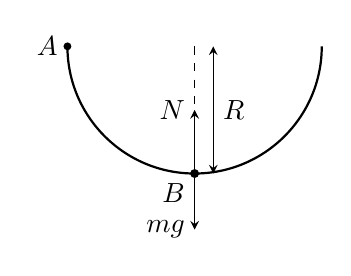
\begin{tikzpicture}[scale=0.95,>=stealth]
  \draw[thick] (-1.7,0) arc (180:360:1.7);
  \draw[dashed] (0,0) -- (0,-1.7);
  \fill (-1.7,0) circle (1.5pt) node[left] {\(A\)};
  \fill (0,-1.7) circle (1.7pt) node[below left] {\(B\)};
  \draw[<->] (0.25,0) -- (0.25,-1.7) node[midway,right] {\(R\)};
  \draw[->] (0,-1.7) -- (0,-0.85) node[left] {\(N\)};
  \draw[->] (0,-1.7) -- (0,-2.45) node[left] {\(mg\)};
\end{tikzpicture}
\end{center}
\end{exercise}

\begin{solution}
\textbf{起手判断/模型：} 题目没有给末速，却给了最低点的支持力 \(N\)。因此先在最低点用径向动力学反推出 \(v_B^2\)，再用动能定理把重力、支持力和摩擦力分账。

\textbf{最低点径向方程：} 在最低点，指向圆心的方向竖直向上，故
\[
N-mg=m\frac{v_B^2}{R}.
\]
于是
\[
v_B^2=R\left(\frac{N}{m}-g\right).
\]

\textbf{全过程能量账：} 从边缘到最低点下降高度为 \(R\)，重力做功
\[
W_g=mgR.
\]
支持力始终沿法向，和瞬时位移垂直，所以
\[
W_N=0.
\]
动能定理给出
\[
W_g+W_N+W_f=\frac12mv_B^2.
\]
代入 \(v_B^2\)：
\[
mgR+W_f=\frac12mR\left(\frac{N}{m}-g\right)
=\frac12R(N-mg).
\]
所以
\[
W_f=\frac12R(N-3mg).
\]

\textbf{结论：}
\[
\boxed{W_f=\frac12R(N-3mg)}.
\]

\textbf{物理检查/易错点：} 若无摩擦，从边缘滑到底部应有 \(v^2=2gR\)，此时最低点 \(N=mg+m v^2/R=3mg\)，公式给出 \(W_f=0\)，极限正确。若有摩擦耗能，则 \(N<3mg\)，摩擦做功为负。
\end{solution}

\begin{exercise}[变力 \(F=4+2t^2\) 作用时为什么仍可先求末速度]
质量为 \(m=\SI{10}{kg}\) 的质点沿 \(x\) 轴无摩擦运动，\(t=0\) 时静止。若所受合力
\[
F=4+2t^2,
\]
求该力在前 \(\SI{3}{s}\) 内所做的功。
\end{exercise}

\begin{solution}
\textbf{起手判断/模型：} 这类题和上一题一样，真正稳定的入口仍是“先由 \(F(t)\) 求末速度，再由动能定理求功”。因为力给成时间函数时，\(\int F\,\dd x\) 并不是最直接的路。

\textbf{主方程：}
\[
F=m\dv{v}{t},\qquad
W=\Delta E_k.
\]

\textbf{分步代入或化简：}
\[
\begin{aligned}
10\dv{v}{t}&=4+2t^2
\implies
\dv{v}{t}=0.4+0.2t^2,\\
\int_0^v \dd v&=\int_0^3 (0.4+0.2t^2)\,\dd t
\implies
v=0.4\times 3+0.2\times \frac{3^3}{3}=\SI{3}{m/s}.
\end{aligned}
\]
于是
\[
W=\frac12\times 10\times 3^2=\SI{45}{J}.
\]

\textbf{结论：}
\[
W=\SI{45}{J}.
\]

\textbf{物理检查/易错点：} 力在全过程中恒正，且物体由静止加速到 \(\SI{3}{m/s}\)，做功为正且量级几十焦耳，合理。易错点同样是把对时间积分的结果误认成做功。
\end{solution}

\begin{exercise}[阻力与深度成正比时子弹能打进多深]
一颗质量为 \(m\) 的子弹以初速度 \(v_0\) 射入固定木板。设木板对子弹的阻力满足
\[
f=-\beta x,
\]
其中 \(x\) 为射入深度，\(\beta\) 为正常数。求子弹射入木板的最大深度。
\end{exercise}

\begin{solution}
\textbf{起手判断/模型：} 题目给的是阻力随位移 \(x\) 的关系，而且最终求的是“打进多深”，所以最稳的入口是\textbf{动能定理}：阻力做的功恰好吃掉子弹初动能。

\textbf{主方程：}
\[
W_f=\Delta E_k.
\]
当子弹恰好停下时，
\[
E_{k,\text{末}}=0,\qquad
E_{k,\text{初}}=\frac12 mv_0^2.
\]

\textbf{分步代入或化简：}
\[
W_f=\int_0^l (-\beta x)\,\dd x=-\frac12 \beta l^2.
\]
于是
\[
-\frac12 \beta l^2=0-\frac12 mv_0^2
\implies
l^2=\frac{mv_0^2}{\beta}
\implies
l=v_0\sqrt{\frac{m}{\beta}}.
\]

\textbf{结论：}
\[
l=v_0\sqrt{\frac{m}{\beta}}.
\]

\textbf{物理检查/易错点：} \(\beta\) 越大，木板“变硬”，射入深度应越小；\(v_0\) 越大，深度应越大，结果都符合直觉。最容易错的是把阻力写成正功，或在积分后漏掉平方根。
\end{solution}

\begin{exercise}[单摆从 \(30^\circ\) 摆到 \(10^\circ\) 时速度怎样自然长出来]
一质量为 \(m\) 的小球系在长为 \(\ell\) 的细绳下端，先由静止释放，初始时绳与竖直方向成 \(\theta_0=30^\circ\)。求当绳与竖直方向成 \(\theta=10^\circ\) 时小球的速率。
\end{exercise}

\begin{solution}
\textbf{起手判断/模型：} 这道题只问某一位置的速率，而且绳张力始终垂直位移不做功，所以最稳的入口是\textbf{机械能守恒}。真正改变动能的只有重力。

\textbf{主方程：}
\[
E_{k1}+E_{p1}=E_{k2}+E_{p2}.
\]
若取最低点为重力势能零点，则摆角为 \(\theta\) 时的高度差为 \(\ell(1-\cos\theta)\)。

\textbf{分步代入或化简：}
\[
\begin{aligned}
0+mg\ell(1-\cos\theta_0)
&=\frac12 mv^2+mg\ell(1-\cos\theta),\\
\implies \frac12 mv^2
&=mg\ell(\cos\theta-\cos\theta_0),\\
\implies
v&=\sqrt{2g\ell(\cos\theta-\cos\theta_0)}.
\end{aligned}
\]
代入 \(\theta_0=30^\circ,\ \theta=10^\circ\) 即得
\[
v=\sqrt{2g\ell\left(\cos10^\circ-\cos30^\circ\right)}.
\]

\textbf{结论：}
\[
v=\sqrt{2g\ell\left(\cos10^\circ-\cos30^\circ\right)}.
\]

\textbf{物理检查/易错点：} 因为 \(10^\circ\) 比 \(30^\circ\) 更接近最低点，速度应为正且不为零；而 \(\cos10^\circ>\cos30^\circ\)，所以根号内为正，判断一致。最容易错的是把高度差写成 \(\ell\cos\theta\) 而漏掉常数项，或把角度顺序写反。
\end{solution}

\section{章末小结}

\summaryline{守恒定律的关键不是背公式，而是先判断系统和条件。系统选错、条件看错，再熟练的代数都会把题做偏。}
\chapterselfcheck{什么时候优先看动量守恒，什么时候优先看机械能守恒？角动量守恒为什么能接到刚体转动？}
\begin{note}
\textbf{把这一章压成三句起手口令最实用：} 碰撞、爆炸、短时相互作用先问外力冲量可否忽略，所以先想动量；题目强调“绕某点或某轴怎样转”时，先问相对该点或该轴的合外力矩，所以先想角动量；题目只关心高度、速度、弹簧压缩量，而过程里又没有非保守力做功时，先想机械能守恒。
\end{note}
\bridge{下一章会把角动量思想进一步推广到刚体：当物体有尺寸和转动轴时，角动量不再只和 \(m\) 与 \(v\) 有关，还要引入转动惯量 \(J\)。}

\begin{exercise}[2003级期末：三角轨道拐角处的冲量]
质量为 \(m\) 的质点以不变速率 \(v\) 沿水平光滑的正三角形轨道运动。质点越过顶角 \(A\) 时，轨道作用于质点的冲量大小是多少？

\begin{center}

\includegraphics[width=0.22\linewidth]{pdf-exercises/pdf2003-q01-triangle.png}
\end{center}
\end{exercise}

\begin{solution}
\textbf{起手判断/模型：} 题目问的是“越过拐角时轨道给的冲量”，而冲量直接等于动量变化量。速率不变并不代表动量不变，因为速度方向在顶角处突变。

\textbf{主方程：}
\[
I=\abs{\Delta \vb*{p}}=m\abs{\vb*{v}_2-\vb*{v}_1}.
\]

\textbf{分步化简：} 正三角形轨道相邻两边夹角为 \(60^\circ\)，但质点在越过顶角时，进入顶角前的速度方向沿一边指向 \(A\)，离开顶角后的速度方向沿另一边离开 \(A\)。这两个速度矢量之间的夹角为 \(120^\circ\)。因此
\[
\abs{\Delta \vb*{v}}
=\sqrt{v^2+v^2-2v^2\cos120^\circ}
=\sqrt{3}\,v.
\]

\textbf{结论：}
\[
\boxed{I=\sqrt{3}\,mv}.
\]

\textbf{物理检查/易错点：} 若把两速度夹角误取成 \(60^\circ\)，会得到 \(mv\)，这是只看几何内角而忘了速度一条是“进顶点”、一条是“出顶点”。冲量看的是速度矢量头尾差，必须画速度方向。
\end{solution}

\begin{exercise}[2006级期末：恒力加速中两段功和冲量怎样比较]
物体在恒力 \(F\) 作用下作直线运动，在时间 \(\Delta t_1\) 内速度由 \(0\) 增加到 \(v\)，在时间 \(\Delta t_2\) 内速度由 \(v\) 增加到 \(2v\)。设 \(F\) 在 \(\Delta t_1\) 内做功为 \(W_1\)、冲量为 \(I_1\)，在 \(\Delta t_2\) 内做功为 \(W_2\)、冲量为 \(I_2\)。比较 \(W_1,W_2\) 与 \(I_1,I_2\)。
\end{exercise}

\begin{solution}
\textbf{起手判断/模型：} 恒力意味着加速度恒定，所以每增加同样的速度所用时间相同；但动能不是和 \(v\) 成正比，而是和 \(v^2\) 成正比，因此两段做功不相同。

\textbf{冲量比较：}
\[
I_1=\Delta p_1=m(v-0)=mv,
\qquad
I_2=\Delta p_2=m(2v-v)=mv.
\]
所以
\[
I_1=I_2.
\]

\textbf{做功比较：} 由动能定理，
\[
W_1=\frac12mv^2-0=\frac12mv^2,
\]
\[
W_2=\frac12m(2v)^2-\frac12mv^2=\frac32mv^2.
\]
因此
\[
W_1<W_2.
\]

\textbf{结论：}
\[
\boxed{W_1<W_2,\qquad I_1=I_2}.
\]

\textbf{物理检查/易错点：} 冲量看动量变化，速度每段都增加 \(v\)，所以相等；功看动能变化，第二段从 \(v\) 到 \(2v\) 的动能增量更大。不要把“同样增速”误判成“同样做功”。
\end{solution}

\begin{exercise}[2007级期末：相同冲量作用下动量增量怎样比较]
质量分别为 \(m_A,m_B\) 且 \(m_A>m_B\) 的两个质点，速度大小分别为 \(v_A,v_B\) 且 \(v_A>v_B\)。若它们受到相同冲量作用，比较两质点动量增量的大小。
\end{exercise}

\begin{solution}
\textbf{起手判断/模型：} 冲量和动量变化之间是定义级关系：
\[
\vb*{I}=\Delta\vb*{p}.
\]
题目已经说两个质点受到相同冲量，因此不需要再比较质量和初速度。

\textbf{结论：}
\[
\boxed{\Delta\vb*{p}_A=\Delta\vb*{p}_B}.
\]
若只比较绝对值，也有
\[
\boxed{\abs{\Delta\vb*{p}_A}=\abs{\Delta\vb*{p}_B}}.
\]

\textbf{物理检查/易错点：} 质量会影响同一冲量造成的速度增量，因为 \(\Delta\vb*{v}=\vb*{I}/m\)；但题目问的是动量增量，它正好等于冲量本身。
\end{solution}

\begin{exercise}[2013级期末：方向不变变力在前 \(2\) 秒内的冲量]
一物体质量为 \(\SI{10}{kg}\)，受到方向不变的力
\[
F=3+4t\quad(\mathrm{SI})
\]
作用。求从开始计时起前 \(\SI{2}{s}\) 内该力的冲量大小。
\end{exercise}

\begin{solution}
\textbf{起手判断/模型：} 冲量是力对时间的累积。题中力的方向不变，所以冲量大小可以直接对力的大小积分；物体质量在本题中并不参与计算。

\textbf{主方程：}
\[
I=\int_0^2 F(t)\,\dd t
=\int_0^2(3+4t)\,\dd t.
\]

\textbf{分步代入或化简：}
\[
I=\left(3t+2t^2\right)_0^2
=6+8
=\SI{14}{N.s}.
\]

\textbf{结论：}
\[
\boxed{I=\SI{14}{N.s}}.
\]

\textbf{物理检查/易错点：} 冲量对时间积分，不是对位移积分；若把 \(F(2)=11\,\si{N}\) 直接乘 \(\SI{2}{s}\)，就把变力错当成了末态恒力。
\end{solution}

\begin{exercise}[2007级期末：沿 \(x\) 轴变力做功]
某质点在力
\[
\vb*{F}=(4+5x)\vb*{i}\quad(\mathrm{SI})
\]
作用下沿 \(x\) 轴运动。求质点从 \(x=0\) 移动到 \(x=\SI{10}{m}\) 的过程中，该力所做的功。
\end{exercise}

\begin{solution}
\textbf{起手判断/模型：} 力随位置变化，不能直接用 \(W=Fs\)。沿 \(x\) 轴运动时，做功就是对 \(F_x\) 关于 \(x\) 积分。

\textbf{主方程：}
\[
W=\int_{0}^{10}F_x\,\dd x
=\int_0^{10}(4+5x)\,\dd x.
\]

\textbf{分步代入或化简：}
\[
W=\left(4x+\frac52x^2\right)_0^{10}
=40+250
=\SI{290}{J}.
\]

\textbf{结论：}
\[
\boxed{W=\SI{290}{J}}.
\]

\textbf{物理检查/易错点：} 该力在 \(0\le x\le10\) 内始终沿 \(+x\) 方向，位移也沿 \(+x\) 方向，所以做功应为正。若用末态力 \(54\,\si{N}\) 乘位移，会把线性变力错当恒力。
\end{solution}

\begin{exercise}[2009级期末：由运动方程用动能定理求外力功]
质量为 \(m=\SI{0.5}{kg}\) 的质点在 \(Oxy\) 平面内运动，运动方程为
\[
x=t,\qquad y=0.5t^2\quad(\mathrm{SI}).
\]
求从 \(t=\SI{2}{s}\) 到 \(t=\SI{4}{s}\) 这段时间内，外力对质点所做的功。
\end{exercise}

\begin{solution}
\textbf{起手判断/模型：} 题目没有直接给力，而是给了运动方程。要求外力做功时，最稳的是先由速度求初末动能，再用动能定理。

\textbf{主方程：}
\[
W=\Delta E_k=\frac12m(v_2^2-v_1^2).
\]

\textbf{分步代入或化简：} 速度分量为
\[
v_x=\dv{x}{t}=1,\qquad v_y=\dv{y}{t}=t.
\]
所以
\[
v^2=v_x^2+v_y^2=1+t^2.
\]
在 \(t=2\,\si{s}\) 与 \(t=4\,\si{s}\) 时，
\[
v_1^2=1+2^2=5,\qquad v_2^2=1+4^2=17.
\]
因此
\[
W=\frac12\times0.5(17-5)=\SI{3}{J}.
\]

\textbf{结论：}
\[
\boxed{W=\SI{3}{J}}.
\]

\textbf{物理检查/易错点：} 外力做功只和动能变化相等，不需要先反推出完整的力。若只看 \(x=t\) 而漏掉 \(y=0.5t^2\)，就会误判速度不变。
\end{solution}

\begin{exercise}[2003级期末：保守力做功的概念判别]
判断下列说法哪些正确：1. 保守力做正功时，系统内相应势能增加；2. 质点运动经过闭合路径时，保守力对质点做功为零；3. 作用力和反作用力大小相等、方向相反，所以两者做功的代数和必为零。
\end{exercise}

\begin{solution}
\textbf{起手判断/模型：} 这类概念题最稳的入口是先把“保守力做功”和“势能变化”的符号关系写出来：
\[
W_{\text{保}}=-\Delta U.
\]

\textbf{逐项判断：}
\[
W_{\text{保}}>0\implies \Delta U<0,
\]
所以第 1 句错误。保守力做功只与初末位置有关，闭合路径初末位置相同，因此
\[
W_{\text{保,闭合}}=0,
\]
第 2 句正确。第 3 句错误，因为作用力和反作用力作用在不同物体上，它们的位移一般并不相同，不能只凭力大小相等、方向相反就推出做功和为零。

\textbf{结论：} 只有第 2 句正确。

\textbf{物理检查/易错点：} “力相反”不能直接推出“功相反”，功还要看各自作用点的位移。概念题里最容易把力的第三定律和功的定义混成一句。
\end{solution}

\begin{exercise}[2003级期末：光滑球面下滑时的加速度]
质量为 \(m\) 的质点置于固定光滑球面的顶点 \(A\)，由静止开始下滑。到达球面上 \(B\) 点时，半径 \(OB\) 与竖直方向夹角为 \(\theta\)。求此时质点加速度的大小。

\begin{center}

\includegraphics[width=0.23\linewidth]{pdf-exercises/pdf2003-q03-sphere.png}
\end{center}
\end{exercise}

\begin{solution}
\textbf{起手判断/模型：} 曲面运动的加速度要拆成切向和法向两部分。切向加速度由重力沿切线方向的分量给出；法向加速度由此时速率决定，速率则由机械能守恒求出。

\textbf{主方程：}
\[
a_\tau=g\sin\theta,\qquad
a_n=\frac{v^2}{R}.
\]

\textbf{分步代入或化简：} 从顶点滑到 \(B\) 点，下降高度为
\[
h=R(1-\cos\theta).
\]
由机械能守恒，
\[
\frac12 mv^2=mgR(1-\cos\theta)
\implies
v^2=2gR(1-\cos\theta).
\]
于是
\[
a_n=\frac{v^2}{R}=2g(1-\cos\theta).
\]
切向与法向互相垂直，所以总加速度大小为
\[
a=\sqrt{a_\tau^2+a_n^2}
=\sqrt{g^2\sin^2\theta+4g^2(1-\cos\theta)^2}.
\]

\textbf{结论：}
\[
\boxed{a=\sqrt{4g^2(1-\cos\theta)^2+g^2\sin^2\theta}}.
\]

\textbf{物理检查/易错点：} 不能只写 \(g\sin\theta\)，那只是切向分量；也不能只写 \(v^2/R\)，那只是法向分量。曲线运动里速度大小和方向都在变，所以两部分都要保留。
\end{solution}

\begin{exercise}[2003级期末：人在船上走动时反推船质量]
湖面上一小船原来静止，船上渔人质量为 \(\SI{60}{kg}\)。若他相对船向船头走了 \(\SI{4.0}{m}\)，但相对湖底只移动了 \(\SI{3.0}{m}\)，忽略水对船的阻力，求小船质量。
\end{exercise}

\begin{solution}
\textbf{起手判断/模型：} 水平方向外力可忽略，系统质心相对湖底不动。人相对船走了 \(\SI{4.0}{m}\)，而相对地只走了 \(\SI{3.0}{m}\)，说明船向反方向退了 \(\SI{1.0}{m}\)。

\textbf{主方程：} 取人前进方向为正，初始质心位置不变，故
\[
m\Delta x_{\text{人}}+M\Delta x_{\text{船}}=0.
\]

\textbf{分步代入或化简：}
\[
60\times 3.0+M\times(-1.0)=0
\implies
M=\SI{180}{kg}.
\]

\textbf{结论：}
\[
\boxed{M=\SI{180}{kg}}.
\]

\textbf{物理检查/易错点：} 人相对船走 \(\SI{4}{m}\)，但相对地只走 \(\SI{3}{m}\)，差出来的 \(\SI{1}{m}\) 正是船的后退距离。最容易错的是把 \(\SI{4}{m}\) 直接当人的地面位移。
\end{solution}

\begin{exercise}[2004级期末：两船上两人依次跳船后的速度方向]
\(A,B\) 两条船质量都为 \(M\)，首尾相靠且都静止在平静湖面上。两船上各有一质量均为 \(m\) 的人。\(A\) 船上的人以相对于 \(A\) 船的速率 \(u\) 跳到 \(B\) 船上，\(B\) 船上的人再以相对于 \(B\) 船的同一速率 \(u\) 跳到 \(A\) 船上。取图示 \(x\) 方向为正，判断最终 \(A,B\) 两船速度 \(v_A,v_B\) 的符号。

\begin{center}

\includegraphics[width=0.24\linewidth]{pdf-exercises/pdf2004-q02-boats.png}
\end{center}
\end{exercise}

\begin{solution}
\textbf{起手判断/模型：} 水平方向外力可忽略，关键不是追每次跳跃的全部数值，而是看每次人与船的相对速度会给哪条船留下反冲动量。

\textbf{第一次跳跃：} \(A\) 船上的人向 \(+x\) 方向跳向 \(B\)。对“人 + \(A\) 船”这一瞬时相互作用系统，\(A\) 船获得反向速度，因此
\[
v_A<0.
\]
人落到 \(B\) 船后，把一部分向 \(+x\) 的动量传给 \(B\) 船，使 \(B\) 船趋向 \(+x\) 运动。

\textbf{第二次跳跃：} 此时 \(B\) 船上的人再向 \(-x\) 方向跳回 \(A\) 船。因为他相对于 \(B\) 船向左跳，\(B\) 船受到的反冲方向仍为 \(+x\)。所以 \(B\) 船最终速度仍满足
\[
v_B>0.
\]
该人落到 \(A\) 船时带来向 \(-x\) 的动量，也不会把 \(A\) 船推成 \(+x\) 方向。

\textbf{结论：}
\[
\boxed{v_A<0,\qquad v_B>0}.
\]

\textbf{物理检查/易错点：} 这题最容易误以为“两个人互相换回来了，所以两船都静止”。实际交换的是人，不是两次冲量完全抵消；每次跳跃对本船的反冲方向要逐次判断。
\end{solution}

\begin{exercise}[2003级期末：拉绳缩短半径后的角速度]
质量为 \(\SI{0.05}{kg}\) 的小块置于光滑水平桌面上，细绳一端连小块，另一端穿过桌面中心小孔。小块原来以 \(\SI{3}{rad/s}\) 的角速度在半径 \(\SI{0.2}{m}\) 的圆周上转动；现将绳从小孔缓慢下拉，使半径减为 \(\SI{0.1}{m}\)。求新的角速度。

\begin{center}

\includegraphics[width=0.25\linewidth]{pdf-exercises/pdf2003-q11-hole.png}
\end{center}
\end{exercise}

\begin{solution}
\textbf{起手判断/模型：} 拉力始终沿半径方向，通过小孔，对小孔的力矩为零，所以绕小孔的角动量守恒。注意这里守恒的是 \(L=mr^2\omega\)，不是 \(r\omega\)。

\textbf{主方程：}
\[
mr_1^2\omega_1=mr_2^2\omega_2.
\]

\textbf{分步代入或化简：}
\[
\omega_2=\omega_1\left(\frac{r_1}{r_2}\right)^2
=3\left(\frac{0.2}{0.1}\right)^2
=\SI{12}{rad/s}.
\]

\textbf{结论：}
\[
\boxed{\omega_2=\SI{12}{rad/s}}.
\]

\textbf{物理检查/易错点：} 半径减半时角速度增为 \(4\) 倍，因为 \(L=mr^2\omega\)。若问线速度，才有 \(rv=\text{常量}\) 或 \(v\propto 1/r\) 的形式。
\end{solution}

\begin{exercise}[2004级期末：两钢球缩短转动半径后的角速度]
如图，质量相等的钢球 \(A,B\) 被绳牵着，以 \(\omega_0=\SI{4}{rad/s}\) 的角速度绕竖直轴转动，二球与轴的距离均为 \(r_1=\SI{15}{cm}\)。现把轴上环 \(C\) 下移，使两球离轴距离缩减为 \(r_2=\SI{5}{cm}\)。求钢球新的角速度。

\begin{center}

\includegraphics[width=0.24\linewidth]{pdf-exercises/pdf2004-q12-steel-balls.png}
\end{center}
\end{exercise}

\begin{solution}
\textbf{起手判断/模型：} 对竖直轴而言，绳的拉力通过轴线或成对对称，系统外力矩可忽略，所以两球绕竖直轴的总角动量守恒。两球质量相等、半径相同，因子 \(2m\) 会约掉。

\textbf{主方程：}
\[
2mr_1^2\omega_0=2mr_2^2\omega.
\]

\textbf{分步代入或化简：}
\[
\omega=\omega_0\left(\frac{r_1}{r_2}\right)^2
=4\left(\frac{15}{5}\right)^2
=\SI{36}{rad/s}.
\]

\textbf{结论：}
\[
\boxed{\omega=\SI{36}{rad/s}}.
\]

\textbf{物理检查/易错点：} 半径缩小到原来的 \(1/3\)，角速度增大到 \(9\) 倍，这是 \(L=J\omega\) 且 \(J\propto r^2\) 的直接结果。最容易错的是只按 \(v=r\omega\) 把角速度放大 \(3\) 倍。
\end{solution}

\begin{exercise}[2004级期末：椭圆轨道远近点的角动量和动能]
人造地球卫星到地球中心 \(O\) 的最大距离和最小距离分别为 \(R_A\) 和 \(R_B\)。设卫星在远地点 \(A\) 与近地点 \(B\) 的角动量分别为 \(L_A,L_B\)，动能分别为 \(E_{KA},E_{KB}\)。判断二者大小关系。

\begin{center}

\includegraphics[width=0.23\linewidth]{pdf-exercises/pdf2004-q03-satellite.png}
\end{center}
\end{exercise}

\begin{solution}
\textbf{起手判断/模型：} 卫星只受地球引力，引力始终指向 \(O\)，对 \(O\) 点力矩为零，所以绕 \(O\) 的角动量守恒。动能大小则要结合总机械能守恒和引力势能随距离的变化判断。

\textbf{角动量判断：}
\[
\sum M_O=0\implies L_A=L_B.
\]

\textbf{动能判断：} 万有引力势能为
\[
U=-\frac{GMm}{r}.
\]
近地点 \(B\) 的 \(r\) 更小，所以
\[
U_B<U_A.
\]
同一条椭圆轨道上机械能 \(E=K+U\) 守恒，因此势能在近地点更低时，动能必须更大：
\[
E_{KB}>E_{KA}.
\]

\textbf{结论：}
\[
\boxed{L_A=L_B,\qquad E_{KA}<E_{KB}}.
\]

\textbf{物理检查/易错点：} 椭圆轨道远近点的速度不同，但角动量仍守恒；半径大时速度小，半径小时速度大。最容易错的是把“角动量守恒”误读成“速率相等”。
\end{solution}

\begin{exercise}[]
一质量为 \(m\) 的物体从高为 \(h\) 的位置由静止自由下落，忽略空气阻力，落到地面时速度多大？
\end{exercise}

\begin{solution}
\textbf{起手判断/模型：} 题目只问下落前后的速度，而且明确忽略空气阻力，所以最稳的入口不是逐时写运动方程，而是直接把“物体 + 地球”看成系统，用\textbf{机械能守恒}连接初末态。

\textbf{主方程与化简：} 取地面为重力势能零点，初态由静止释放，故 \(E_{k1}=0\)、\(E_{p1}=mgh\)、\(E_{p2}=0\)。于是
\[
E_{p1}+E_{k1}=E_{p2}+E_{k2}
\implies mgh=\frac{1}{2}mv^2
\implies gh=\frac{v^2}{2}
\implies v=\sqrt{2gh}.
\]

\textbf{结论：} 落到地面时的速率为 \(v=\sqrt{2gh}\)，方向竖直向下。

\textbf{物理检查/易错点：} \(\sqrt{gh}\) 的量纲是 \(\si{m/s}\)，结果量纲正确；质量 \(m\) 被约掉，说明在忽略阻力时落地速率只由高度决定。容易错的地方是把“自由落体”机械地改用动量守恒，但这里并没有“系统外力可忽略”这一条件，真正可用的是重力势能与动能的转化。
\end{solution}

\begin{exercise}[]
若某系统在一段过程中所受合外力矩为零，则哪个物理量守恒？
\end{exercise}

\begin{solution}
\textbf{起手判断/模型：} 这是一道守恒判据题，关键不是“转得快不快”，而是题目已经明确给出\textbf{哪一类外作用为零}。既然给的是合外力矩为零，就应立刻切到角动量定理。

\textbf{主方程与化简：} 对同一参考点或同一转轴，
\[
\dv{\vb*{L}}{t}=\vb*{M}_{\text{外}},\qquad
\vb*{M}_{\text{外}}=0
\implies
\dv{\vb*{L}}{t}=0
\implies
\vb*{L}=\text{常量}.
\]

\textbf{结论：} 守恒的物理量是\textbf{系统对该参考点或该转轴的总角动量}。

\textbf{物理检查/易错点：} “合外力矩为零”不等于“合外力为零”，因此这里推出的是角动量守恒，不是动量守恒；它也不自动推出机械能守恒，因为外力矩为零并不代表过程里没有耗散。
\end{solution}

\begin{exercise}[2005级期末：圆周路径上位置相关力做功]
一质点在如图所示的坐标平面内作圆周运动，有一力
\[
\vb*{F}=F_0(x\vb*{i}+y\vb*{j})
\]
作用在质点上。质点从坐标原点 \(O\) 运动到 \((0,2R)\) 的过程中，求该力所做的功。

\begin{center}

\includegraphics[width=0.22\linewidth]{pdf-exercises/pdf2005-q04-circle-work.png}
\end{center}
\end{exercise}

\begin{solution}
\textbf{起手判断/模型：} 题目虽然画了圆周路径，但力场
\(\vb*{F}=F_0(x\vb*{i}+y\vb*{j})\) 恰好是一个梯度型力场。做功可直接写成线积分，并且只与初末两点的 \(x^2+y^2\) 有关。

\textbf{主方程：}
\[
W=\int_C \vb*{F}\cdot\dd\vb*{r}
=F_0\int_C (x\,\dd x+y\,\dd y).
\]

\textbf{分步代入或化简：}
\[
x\,\dd x+y\,\dd y=\frac12\dd(x^2+y^2),
\]
所以
\[
W=\frac{F_0}{2}\left[(x^2+y^2)_{\text{末}}-(x^2+y^2)_{\text{初}}\right].
\]
初态为 \((0,0)\)，末态为 \((0,2R)\)，于是
\[
W=\frac{F_0}{2}\left(4R^2-0\right)=2F_0R^2.
\]

\textbf{结论：}
\[
\boxed{W=2F_0R^2}.
\]

\textbf{物理检查/易错点：} 这题最容易被“圆周运动”四个字带偏，去硬算圆弧参数。其实该力做功只看 \(x^2+y^2\) 的初末变化；若沿另一条路径从 \(O\) 到同一终点，结果仍相同。
\end{solution}

\begin{exercise}[2005级期末：万有引力做功只看距离变化]
质量分别为 \(m_1,m_2\) 的两质点从相距 \(a\) 变到相距 \(b\)。求二者间万有引力所做的功。
\end{exercise}

\begin{solution}
\textbf{起手判断/模型：} 万有引力是保守力，所以做功可由引力势能变化给出。两质点间的势能只依赖相对距离 \(r\)，而不依赖具体路径。

\textbf{主方程：}
\[
U(r)=-\frac{Gm_1m_2}{r},\qquad
W_g=-\Delta U.
\]

\textbf{分步代入或化简：}
\[
W_g=-\left[-\frac{Gm_1m_2}{b}+\frac{Gm_1m_2}{a}\right]
=Gm_1m_2\left(\frac1b-\frac1a\right).
\]

\textbf{结论：}
\[
\boxed{W_g=Gm_1m_2\left(\frac1b-\frac1a\right)}.
\]

\textbf{物理检查/易错点：} 若 \(b<a\)，两质点互相靠近，引力做正功；代入上式也确为正。若把势能写成 \(+Gm_1m_2/r\)，符号会整个反掉。
\end{solution}

\chapter{刚体力学}

\begin{skill}[第4章冲刺总手册]\label{sk:phys-ch04-overview}
\textbf{【这章先解决什么题】} 这章处理“物体不能再当质点”的题：杆、盘、轮、滑轮、转轴、滚动、陀螺、线圈式转动题。核心是把平动的语言换成转动的语言，再看它们怎样耦合。

\textbf{【拿题先认什么信号】} 若题目出现“绕定轴转动、转动惯量、力矩、角速度、角加速度、滑轮、滚动不滑、进动”，就进入刚体模型；若题目同时有质点和平动部件，又有转动物体，就准备联立平动方程、转动方程和约束条件。

\textbf{【第一条方程先写什么】}
\[
\sum M=J\alpha.
\]
先把转轴选好，再给每个力矩定正负。若题目还有平动部分，就再补
\[
\sum F=ma.
\]

\textbf{【必背公式块】}
\[
\begin{aligned}
L&=J\omega,\qquad
M=\dv{L}{t},\qquad
\sum M=J\alpha\ \text{(定轴且 \(J\) 不变)},\\
K_{\text{rot}}&=\frac12 J\omega^2,\qquad
W=\Delta\!\left(\frac12 J\omega^2\right),\\
J&=J_C+md^2\ \text{(平行轴定理)},\\
v&=\omega R,\qquad
a=\alpha R\ \text{(纯滚动约束)}.
\end{aligned}
\]
其中 \(J\) 是相对所选转轴的转动惯量，不是物体的“唯一常数”。

\textbf{【做题流程】} 先定研究对象和转轴；再算各力对该轴的力矩；若是滑轮、滚动、复合系统，就同时写 \(\sum F=ma\)、\(\sum M=J\alpha\)、\(a=\alpha R\) 或 \(v=\omega R\)；若只问初末态速度，可优先考虑转动动能和机械能守恒；若问某点是否守恒角动量，先检查该点外力矩是否为零。

\textbf{【最容易误判】} 转轴选错；把不同半径或不同部件的 \(a,\alpha,\omega\) 误写成同一个量；滚动题只写转动动能、忘了质心平动动能；默认滑轮两侧张力相等，而题目明明有转动惯量。

\textbf{【最后怎样验证】} 看力矩单位是否为 \(\si{N.m}\)，转动惯量单位是否为 \(\si{kg.m^2}\)；滚动题最后检查是否满足 \(v=\omega R\)；若物体离转轴越远算出的 \(J\) 反而更小，说明公式或轴选错了。
\end{skill}

\chapterroadmap
{当物体不能再被当作一个点时，怎样把“转动”单独描述出来，并把它和前面学过的角动量、功和机械能重新接起来。}
{已经掌握位移、速度、加速度、受力分析、角动量和机械能守恒等基本思想。}
{新增刚体模型、定轴转动、转动惯量、角动量定理、转动动能、复合系统和回转运动。}

\bridge{这一章最容易让人掉线的地方，不是公式多，而是观察视角突然变了：前面更多是在盯“一个点怎么动”，现在要盯“整个物体相对某条轴怎么动”。只要始终记住平动和转动之间的对应关系，刚体章就不会散。}

\section{为什么质点模型不够用了}

前面几章之所以能把物体看成质点，是因为我们主要关心“整体往哪里走”。可是一旦物体开始明显地绕轴转动，光知道质心的位置已经不够了。门绕合页转动、车轮滚动、飞轮储能，都在提醒我们：\textbf{同一个物体上的不同点，虽然属于同一整体，但它们的速度大小、速度方向和受力效果都可能不同。}

这就是刚体力学要解决的核心问题：当物体有大小时，怎样把“整体平动”和“绕轴转动”同时描述清楚。从这里开始，我们不再只问“物体有没有加速度”，还要问“它绕哪条轴转”“转得快不快”“这种转动状态难不难改变”。

\begin{note}
如果你觉得这一章突然变抽象，这是正常的。真正新增的不是很多公式，而是观察物体的视角：从只盯住一个点，变成盯住整个物体相对某条轴的运动。
\end{note}

\section{刚体的基本运动形式：平动、转动、一般运动}

这一节要解决的问题是：刚体的运动到底有哪些基本类型，我们这一章究竟只研究其中哪一类？

前面质点模型故意忽略物体的大小，只追“整体到哪了、速度多大”。可一旦题目开始关心门为什么更适合从把手处推开、飞轮为什么难以加速、杆上不同点为什么快慢不同，物体的尺寸和质量分布就再也藏不住了。也就是说，这时真正要追的不只是“物体作为一个整体怎么走”，还要追“物体各部分相对某条轴怎样转”。这正是刚体模型登场的原因。

\begin{itemize}
  \item \textbf{平动：} 刚体中所有点的轨迹彼此完全相同，或者说刚体内任意两点的连线在运动过程中始终保持平行。此时虽然物体有大小，但整体运动效果和质点很像。
  \item \textbf{转动：} 刚体绕某条轴或某个定点旋转，物体上不同点到轴的距离不同，因此速度和加速度通常也不同。
  \item \textbf{一般运动：} 既有质心的平动，又有绕质心的转动。可以把它理解成“整体在走，同时自己也在转”。
\end{itemize}

\begin{note}
\textbf{这里不要把三类运动看成三张孤立定义卡。} 更稳的理解顺序是：先问“物体内部各点彼此之间的相对位置有没有只做平移”，若是，就偏向平动；若明显在绕某条轴扫角度，就偏向转动；若两种特征同时存在，就是一般运动。也正因为一般运动最复杂，所以本章故意先把问题压到最稳定的入口模型：定轴转动。
\end{note}

\begin{note}
一般运动在更完整的刚体力学里非常重要，但最稳定的入口仍然是\textbf{定轴转动}。因为一旦转轴固定，角位移、角速度、角加速度这三件事就都能稳定地定义下来，很多抽象量也会立刻变得可算。
\end{note}

\section{刚体与定轴转动}

刚体并不是说真实物体绝对不会形变，而是说在当前问题里，这点形变小到可以忽略，于是物体内部任意两点间距离可以近似看成不变。我们之所以第一次学刚体时优先盯住\textbf{定轴转动}，是因为一般刚体运动往往同时含有平动和转动，而一旦先把转轴固定，整块物体的公共运动状态就能压成一个角坐标来记，后面的角速度、角加速度、力矩和转动惯量才会一起稳定下来。

\begin{definition}[刚体]\label{def:rigid-body}
在受力过程中，物体内部任意两点之间距离始终保持不变的理想模型称为\textbf{刚体}。
\end{definition}

真实物体都会有形变，但若形变很小、对问题影响可以忽略，就可以近似看成刚体。

\begin{definition}[定轴转动]\label{def:fixed-axis-rotation}
若刚体绕一条固定不动的轴转动，则称为\textbf{定轴转动}。
\end{definition}

\begin{note}
这一定义看起来朴素，但它其实在帮我们把复杂刚体问题大幅降维：一旦转轴固定，整块刚体的运动就能主要用一个角坐标 \(\theta\) 来描述，后面的 \(\omega,\alpha,J,M\) 才能稳定地围绕同一根轴定义。也正因为如此，定轴转动是第一次学刚体时最可靠的入口模型。
\end{note}

\begin{note}
\textbf{做刚体题时有个动作必须更早：} 先把“绕哪条轴”圈出来。对同一个刚体，转轴一换，后面的 \(r\)、\(J\)、\(L\)、\(M\) 往往都会跟着变；真正能在整块刚体上共享的，只有围绕\textbf{同一根固定轴}定义出来的 \(\theta,\omega,\alpha\)。所以“同一物体”并不等于“同一道转动题”。
\end{note}

门绕合页转动、唱片绕转轴旋转、滑轮绕中心轴转动，都是定轴转动。它是刚体力学中最基础、也最适合建立平动与转动对应关系的模型。

\section{角位移、角速度、角加速度}

在定轴转动里，整块刚体虽然各点线速度不同，但每个点在同一时刻都共同转过同一个角 \(\theta\)。所以真正先被整块刚体共享的是角量，不是线量；线速度、切向加速度这些量，只是把公共的角状态按离轴距离 \(r\) 翻译成各点自己的局部结果。于是刚体定轴转动时，可以用下面这组角量来描述转动状态：
\[
\begin{aligned}
\theta,\qquad \omega&=\dv{\theta}{t},\qquad \alpha=\dv{\omega}{t},\\
v&=r\omega,\qquad a_\tau=r\alpha,\qquad a_n=r\omega^2,\\
\vb*{v}_i&=\vb*{\omega}\times \vb*{r}_i.
\end{aligned}
\]
这里的逻辑和直线运动完全平行：位置对应角位置，速度对应角速度，加速度对应角加速度；若刚体上某点到转轴距离为 \(r\)，它的线量就按上式和角量接通。

\bridge{定轴转动里最省心的一点是：同一刚体上所有点在同一时刻具有相同的 \(\theta\)、\(\omega\) 和 \(\alpha\)，不同的只是离轴距离 \(r\)。因此越远离转轴的点，线速度和法向加速度通常越大。}

\begin{note}
\textbf{为什么这里先写角量，再写线量？} 因为定轴转动里真正由整块刚体共同“共享”的，是转过多少角、转得多快、快慢变得多快；某一点的线速度和线加速度，只是把这组公共角量乘上了它自己的离轴距离 \(r\) 之后得到的局部版本。先看角量，等于先抓整块刚体的公共主线；再看线量，等于把主线翻译回某个具体点。
\end{note}

\section{力矩}

平动里我们关心“力把物体往哪推、推得多厉害”；转动里真正该先问的是“这股力到底有没有把物体拧起来，以及拧得有多厉害”。同样大小的力，若作用点更远、方向更合适，转动效果就会更强；若力的作用线恰好穿过转轴，它再大也拧不动。所以转动里不能只记 \(F\) 本身，必须把“力施加在离轴多远的地方”一起记账，这就得到力矩。第 3 章已经把力矩定义为 \(\vb*{M}=\vb*{r}\times\vb*{F}\)。进入定轴转动后，我们不再重复定义本身，只把它固定到同一转轴上来使用：
\[
\vb*{M}=\vb*{r}\times \vb*{F},\qquad
M=rF\sin\theta=Fl,
\]
其中 \(l\) 是力臂，也就是力的作用线到转轴的垂直距离。

\begin{note}
这里要先分清三层：\(\vb*{M}=\vb*{r}\times\vb*{F}\) 是矢量定义；\(M=rF\sin\theta=Fl\) 给的是大小；真正到定轴列方程时，再先约定顺时针或逆时针哪个为正，把各力矩写成带正负号的代数量。若这三层不先分开，后面的 \(\alpha\) 正负号通常会乱。
\end{note}

\section{刚体定轴转动的角动量}

第 3 章已经定义了质点角动量。本章只需把它对同一转轴上的所有质元求和。这里最好先说清一个默认前提：\textbf{定轴转动时，各质元角动量都平行于同一转轴，差别只在大小与正负方向，所以可以按统一正方向代数求和。} 正因为方向不会乱，下面的求和才会压成一个简单的标量公式：
\[
\begin{aligned}
L_i&=r_i m_i v_i=r_i m_i(r_i\omega)=m_i r_i^2\omega,\\
L&=\sum_i L_i=\sum_i m_i r_i^2\omega
=\left(\sum_i m_i r_i^2\right)\omega=J\omega.
\end{aligned}
\]

\begin{definition}[刚体定轴转动的角动量]
刚体绕固定轴转动时，若其对该轴的转动惯量为 \(J\)，角速度为 \(\omega\)，则它对该轴的角动量为 \(L=J\omega\)。
\end{definition}

\begin{note}
这里把第 3 章的矢量角动量，在定轴情形下压成了沿该轴记账的标量 \(L=J\omega\)；同时仍要分清：力矩 \(M\) 是改变转动状态的原因，角动量 \(L\) 是当前转动状态的量度。
\end{note}

\section{转动惯量}

\textbf{先把积分对象说清楚，再看定义。} 刚体不是一个点，所以不能只拿总质量去记“绕轴有多难转”。最稳的方法是把刚体切成很多小质量元：每一小块质量记成 \(\dd m\)，它到所选转轴的垂直距离记成 \(r\)，它对转动状态的贡献就按 \(r^2\,\dd m\) 加权；最后在整块物体上把这些贡献加总，才得到转动惯量。

\begin{definition}[转动惯量]\label{def:moment-of-inertia}
刚体对某转轴的转动惯量定义为
\[
J=\sum_i m_i r_i^2,\qquad
\text{连续分布时 }J=\int r^2\,\dd m.
\]
\end{definition}

\textbf{这个定义也不是凭空拍出来的。} 要理解它为什么是 \(r^2\)，最稳的方法是先从已经得到的刚体角动量公式倒推。对第 \(i\) 个质元，
\[
L_i=r_i m_i v_i.
\]
而定轴转动时，每个质元的线速度都不是独立的，它们共享同一个角速度 \(\omega\)，并满足
\[
v_i=r_i\omega.
\]
代入后就得到
\[
L_i=r_i m_i(r_i\omega)=m_i r_i^2\omega.
\]
也就是说，\textbf{同一角速度 \(\omega\) 下，某一小块质量对整体转动状态的贡献天然就按 \(m_i r_i^2\) 加权。} 于是把所有质元加总时，公共的 \(\omega\) 可以提出来，剩下那一坨只依赖“质量怎样分布在转轴周围”的系数，便定义为转动惯量 \(J\)。

\begin{note}
\textbf{为什么不是 \(mr\)，也不是单纯总质量 \(m\)？}
如果只按 \(mr\) 加权，那么离轴两倍远的质量只会贡献两倍影响；但真实转动里，离轴两倍远的同一质量，不仅“胳膊更长”，它本身的线速度也会随 \(v=r\omega\) 再多出一个 \(r\)。一个 \(r\) 来自“离轴更远”，另一个 \(r\) 来自“同角速度下跑得更快”，两者一乘才得到 \(r^2\)。这也是为什么同质量、同半径的圆盘和圆环，圆环更难转起来：不是它更重，而是它把更多质量放到了更大的 \(r\) 上。
\end{note}

\bridge{从 \(\sum m_i r_i^2\) 到 \(\int r^2\,\dd m\)，只是把”许多小质量块逐个相加”改写成连续积分。这里的 \(r\) 永远指质量元到\textbf{所选转轴的垂直距离}，\(\dd m\) 则按线密度、面密度或体密度去取；因此 \(J\) 绝不是简单拿”总质量乘某个半径平方”就能代替。}

\begin{remark}
如何把 \(\dd m\) 写成可积分的形式？关键是引入密度：
\begin{itemize}
\item 一维细杆：线密度 \(\lambda\)，则 \(\dd m=\lambda\,\dd l\)（\(\dd l\) 为长度元）；
\item 二维薄板/壳：面密度 \(\sigma\)，则 \(\dd m=\sigma\,\dd S\)（\(\dd S\) 为面积元）；
\item 三维实体：体密度 \(\rho\)，则 \(\dd m=\rho\,\dd V\)（\(\dd V\) 为体积元）。
\end{itemize}
对均匀物体，密度为常数，可以提到积分号外面。例如均匀细杆 \(\lambda=m/L\)，均匀圆盘 \(\sigma=m/(\pi R^2)\)。设置好 \(\dd m\) 后，\(J=\int r^2\,\dd m\) 就变成了关于几何坐标的普通定积分。
\end{remark}

把 \(J\) 理解成“质量分布对转轴的 \(r^2\) 加权结果”最容易接受：离轴越远的质量，权重按平方放大，所以对转动状态的影响也越大。它不是总质量的别名，而是“这套质量分布绕这根轴有多难转起来”的量化。

它衡量的是刚体“改变转动状态的难易程度”。在平动里，质量越大越难改变速度；在转动里，转动惯量越大越难改变角速度。

但转动惯量和质量又不完全一样。质量只告诉我们“东西有多少”，转动惯量还要继续追问“这些质量分布在离转轴多远的地方”。因此，转动惯量取决于三件事：
\begin{itemize}
  \item 总质量有多大；
  \item 质量怎样分布；
  \item 转轴选在哪里。
\end{itemize}

\begin{note}
同质量、同半径的实心圆盘和薄圆环，圆环的质量分布离轴更远，所以转动惯量更大；同一根细杆绕中点转和绕端点转，转动惯量也会不同。做题时只要看到“换轴”，就要立刻警惕 \(J\) 是否改变。
\end{note}

\begin{exercise}
质量为 \(m\)、半径为 \(R\) 的质点绕圆心转动，其转动惯量为 \(J=mR^2\)。
\end{exercise}

\section{转动惯量的计算}

这一节要解决的问题是：一旦刚体不是几个离散质点，而是连续分布的物体，转动惯量该怎么求？

\bridge{为什么非要精确算出 \(J\)？因为转动动能 \(E_k=\frac12 J\omega^2\) 和角动量 \(L=J\omega\) 都直接依赖它。如果 \(J\) 只是"大概知道"，那能量守恒和角动量守恒就没法定量使用。所以这一节的目标很明确：给定一个连续质量分布和一根转轴，把 \(J\) 算出来。}

\bridge{转动惯量的陌生感主要来自“质量分布”第一次进入计算。最稳的办法是：先把刚体切成很多小质量元，再把每一小块对转轴的贡献 \(r^2\,\dd m\) 全部加起来。}

统一模板固定为三步：
\begin{enumerate}
  \item 先选合适的质量元 \(\dd m\)；
  \item 再写出该质量元到转轴的距离 \(r\)；
  \item 最后用 \(\dd J=r^2\,\dd m\) 积起来。
\end{enumerate}

\begin{note}
\textbf{这三步里最关键的其实是前两步。} 真正把题做对的，往往不是后面的积分技巧，而是有没有先选到“同一小块上 \(r\) 最简单”的切法。细杆常切长度元，圆盘常切同心薄环，球体常切薄球壳；本质上都在做同一件事：让 \(\dd m\) 和 \(r\) 尽量同时写得干净。
\end{note}

\begin{exercise}[均匀细杆绕中心的转动惯量]
求质量为 \(m\)、长度为 \(\ell\) 的均匀细杆，绕通过中点且垂直于杆的轴的转动惯量。
\end{exercise}

\begin{solution}
\textbf{起手判断/模型：} 题目问的是连续质量分布刚体绕已知轴的转动惯量，最先要回到定义
\(J=\int r^2\,\dd m\)，而不是直接背结果。因为这里真正决定 \(J\) 的，是质量元离转轴有多远。

\textbf{主方程与化简：} 把细杆放在 \(x\) 轴上，中点取为原点，转轴垂直于杆并过中点，则
\[
\begin{aligned}
\lambda&=\frac{m}{\ell},\qquad \dd m=\lambda\,\dd x,\qquad r=\abs{x},\qquad
\dd J=r^2\,\dd m=x^2\lambda\,\dd x,\\
J_C&=\int_{-\ell/2}^{\ell/2}x^2\lambda\,\dd x
=\frac{m}{\ell}\int_{-\ell/2}^{\ell/2}x^2\,\dd x
=\frac{m}{\ell}\left[\frac{x^3}{3}\right]_{-\ell/2}^{\ell/2}
=\frac{1}{12}m\ell^2.
\end{aligned}
\]

\textbf{结论：} 均匀细杆绕中心、垂直于杆的轴的转动惯量为 \(J_C=\frac{1}{12}m\ell^2\)。

\textbf{物理检查/易错点：} 结果量纲是 \(\si{kg.m^2}\)，正确；被积式里的 \(x^2\) 说明左右两侧贡献同号，所以不能把正负位置当成相互抵消。最容易错的是把 \(r\) 误写成整根杆长 \(\ell\)，或者忘记 \(\dd m\) 要先用线密度改写。
\end{solution}

\section{平行轴定理}

\textbf{这一节先要解决的，不是记住一个新公式，而是回答：同一刚体换一根平行轴后，为什么转动惯量一定会变大，而且恰好多出一项 \(md^2\)？} 既然每个质元到新轴的距离都整体偏移了 \(d\)，那它们的 \(r^2\) 加权总和当然也会整体抬高；平行轴定理正是在把这件事定量写出来。

\begin{theorem}[平行轴定理]\label{thm:parallel-axis}
质量为 \(m\) 的刚体，若绕通过质心的某轴的转动惯量为 \(J_C\)，则绕任一与该轴平行、相距 \(d\) 的轴的转动惯量为 \(J=J_C+md^2\)。
\end{theorem}

\begin{note}
为什么会多出 \(md^2\)？可以把新轴看成在质心轴基础上整体平移了 \(d\)。每个质元离轴距离的平方都会多出一个平均贡献，而关于质心的”偏心项”会互相抵消，最后只剩下整块质量贡献出的 \(md^2\)。

\textbf{证明思路：} 设质心在原点，新轴沿 \(x\) 方向平移了 \(d\)。质元 \(i\) 到质心轴距离为 \(r_i\)，到新轴距离为 \(r_i'\)。展开 \(r_i'^2=(r_i+d\cos\alpha_i)^2+\cdots\) 后求和，交叉项 \(\sum m_i r_i\cos\alpha_i\) 恰好是质心坐标乘以总质量——而质心在原点，所以交叉项为零，只剩 \(J_C+md^2\)。
\end{note}

\begin{remark}
这条定理只适用于\textbf{两条互相平行的轴}。一旦换轴但不平行，就不能直接套它。
\end{remark}

\begin{note}
\textbf{把它当成题面信号最实用：} 只要同一刚体同时出现“绕质心轴”和“绕端点轴/边缘轴/偏移轴”，先别急着重积分，先问这两条轴平不平行。若平行，就直接把平移轴这件事翻成 \(J=J_C+md^2\)；也正因为多出来的是 \(md^2>0\)，所以在一组平行轴里，\textbf{过质心的那条轴总是最“省”转动惯量的入口。}
\end{note}

\begin{exercise}[细杆绕端点的转动惯量]
质量为 \(m\)、长度为 \(\ell\) 的均匀细杆，求它绕通过中点且垂直于杆的轴，以及绕一端且垂直于杆的轴的转动惯量。
\end{exercise}

\begin{solution}
细杆绕中点的结果已经求出：
\[
\begin{aligned}
J_C&=\frac{1}{12}m\ell^2,\\
J_O&=J_C+md^2
=\frac{1}{12}m\ell^2+m\left(\frac{\ell}{2}\right)^2
=\frac13 m\ell^2
\qquad \left(d=\frac{\ell}{2}\right).
\end{aligned}
\]

这道题是平行轴定理最常见的入口。看到“绕中点”和“绕端点”同时出现时，优先想能不能用它把两个结果连起来。
\end{solution}

\section{几种常见刚体的转动惯量推导}

这一节要解决的问题是：为什么教材和公式表里总出现那几个熟悉的结果，它们到底是怎么来的？

\begin{note}
\textbf{先看什么信号：} 题目若不是让你直接套表，而是让你“推一个刚体的 \(J\)”，起手永远回到 \(J=\int r^2\,\dd m\)；\textbf{这条公式在控制什么：} 它控制的是每一小块质量离转轴有多远，离轴越远，贡献越大；\textbf{怎样最快记住：} 先找哪种切片能让同一小块上的 \(r\) 最简单，再决定切成薄环、薄壳还是薄片；\textbf{最容易错：} 还没看清 \(r\) 是到\textbf{所选转轴的垂直距离}，就把总质量直接乘某个半径平方。
\end{note}

\begin{exercise}[细圆环与均匀圆盘]
求质量为 \(m\)、半径为 \(R\) 的均匀细圆环，以及质量为 \(m\)、半径为 \(R\) 的均匀圆盘，绕通过中心且垂直盘面的轴的转动惯量。
\end{exercise}

\begin{solution}
\textbf{细圆环：} 环上各点到转轴的距离都等于 \(R\)，因此
\[
\dd J=R^2\,\dd m
\implies
J=\int \dd J=\int R^2\,\dd m=R^2\int \dd m=mR^2.
\]

\textbf{均匀圆盘：} 圆盘上不同位置离轴距离不同，不能像圆环那样直接把 \(R^2\) 提出来。最自然的切法，是把圆盘看成许多同心薄圆环叠起来。这样切的好处是：同一薄环上每一点离轴距离都相同，仍能保住“这一小层上的 \(r\) 是常量”这个优点。若面密度为
\[
\begin{aligned}
\sigma&=\frac{m}{\pi R^2},\\
\dd m&=\sigma\cdot 2\pi r\,\dd r,\\
\dd J&=r^2\,\dd m=2\pi\sigma r^3\,\dd r,\\
J&=\int_0^R 2\pi\sigma r^3\,\dd r
=2\pi\sigma\cdot \frac{R^4}{4}
=\frac12 mR^2.
\end{aligned}
\]

这两个结果最值得比较的地方在于：两者质量和半径都相同，但圆环的质量更集中在外圈，所以它的转动惯量更大。
\end{solution}

\begin{exercise}[薄球壳与均匀实心球]
求质量为 \(m\)、半径为 \(R\) 的薄球壳，以及质量为 \(m\)、半径为 \(R\) 的均匀实心球，绕直径的转动惯量。
\end{exercise}

\bridge{下面的推导用到了球坐标中的面积元和体积元。如果你还没学过多元微积分，可以先接受以下两个几何事实：(1) 球面上纬度角为 \(\theta\)、宽度为 \(\dd\theta\) 的一条纬线带，面积为 \(\dd S=2\pi R\sin\theta\cdot R\,\dd\theta=2\pi R^2\sin\theta\,\dd\theta\)（想象把纬线带展开成一条长 \(2\pi R\sin\theta\)、宽 \(R\,\dd\theta\) 的窄矩形）；(2) 半径为 \(r\)、厚度为 \(\dd r\) 的薄球壳体积为 \(4\pi r^2\,\dd r\)（球面面积乘以厚度）。有了这两条，下面的积分就只是一元定积分。}

\begin{solution}
\textbf{薄球壳：} 取通过球心的直径为转轴，把球壳看成许多纬线薄圆环叠起来。设纬线与转轴夹角为 \(\theta\)，则
\begin{align*}
r&=R\sin\theta,\qquad
\dd S=2\pi r\cdot R\,\dd\theta=2\pi R^2\sin\theta\,\dd\theta,\qquad
\sigma=\frac{m}{4\pi R^2},\\
\dd m&=\sigma\,\dd S=2\pi\sigma R^2\sin\theta\,\dd\theta,\\
\dd J&=r^2\,\dd m=2\pi\sigma R^4\sin^3\theta\,\dd\theta,\\
J&=\int_0^\pi 2\pi\sigma R^4\sin^3\theta\,\dd\theta
=2\pi\sigma R^4\cdot \frac{4}{3}
=\frac{2}{3}mR^2.
\end{align*}

\textbf{均匀实心球：} 最稳的切法不是切薄圆环，而是把球体看成许多同心薄球壳叠起来。设体密度为 \(\rho\)，则半径为 \(r\)、厚度为 \(\dd r\) 的薄球壳满足
\begin{align*}
\rho&=\frac{m}{\frac43\pi R^3}=\frac{3m}{4\pi R^3},\\
\dd m&=4\pi\rho r^2\,\dd r,\\
\dd J&=\frac23 r^2\,\dd m=\frac{8\pi}{3}\rho r^4\,\dd r,\\
J&=\int_0^R \frac{8\pi}{3}\rho r^4\,\dd r
=\frac{8\pi}{3}\rho\cdot \frac{R^5}{5}
=\frac{8\pi}{15}\rho R^5
=\frac25 mR^2.
\end{align*}

这两个结果也很适合做直觉比较：同半径、同质量时，薄球壳的质量全部分布在外层，所以它的转动惯量大于实心球。
\end{solution}

\begin{center}
\begin{tabular}{c|c}
刚体与转轴 & 转动惯量 \\
\hline
均匀细杆，绕中心垂直于杆 & \(J=\dfrac{1}{12}m\ell^2\) \\
均匀细杆，绕端点垂直于杆 & \(J=\dfrac{1}{3}m\ell^2\) \\
薄圆环或薄圆筒，绕中心轴 & \(J=mR^2\) \\
均匀圆盘或圆柱体，绕中心轴 & \(J=\dfrac12 mR^2\) \\
薄球壳，绕直径 & \(J=\dfrac23 mR^2\) \\
均匀实心球，绕直径 & \(J=\dfrac25 mR^2\)
\end{tabular}
\end{center}

\begin{remark}
这张表不是让你死背所有数字，而是训练一个直觉：质量分布越靠外，转动惯量越大。所以同半径、同质量时，薄圆环 \(>\) 圆盘；薄球壳 \(>\) 实心球。
\end{remark}

\section{刚体定轴转动的角动量定理与转动定律}

这一节要解决的问题是：转动里的“牛顿第二定律”到底是什么，它和角动量定理是什么关系？

这里还要先补一句定轴情形下的记号约定：既然我们始终围绕\textbf{同一固定转轴}讨论转动，\(\vb*{M}\) 和 \(\vb*{L}\) 都只会沿这条轴取正或取负，所以后面完全可以先约定一个正方向，再把它们记成代数量 \(M,L\)。

\begin{theorem}[刚体定轴转动的角动量定理]\label{thm:rigid-body-angular-momentum-theorem}
对选定转轴，作用在刚体上的合外力矩等于刚体对该轴角动量的时间变化率：
\[
M=\dv{L}{t}
\implies
\int_{t_1}^{t_2} M\,\dd t=L_2-L_1.
\]
\end{theorem}

接下来最该先记住的是：这条式子才是本章真正的\textbf{根公式}。它和直线运动中的 \(F=\dv{p}{t}\) 完全平行，都是“外作用改写运动状态量变化率”这同一层结构在不同模型里的表达。定轴转动时，若转轴固定、质量分布相对转轴也不变，则 \(J\) 为常量，这时角动量才进一步压成
\[
L=J\omega
\implies
M=\dv{L}{t}
=\dv{(J\omega)}{t}
=J\dv{\omega}{t}
=J\alpha.
\]
这样读最不容易乱：先有总规律 \(M=\dv{L}{t}\)，再在“同一固定轴、同一个 \(J\)”这两个额外条件下，把它压成熟悉的计算式 \(M=J\alpha\)。所以 \(M=J\alpha\) 不是凭空新增的第二条根公式，而只是角动量定理在定轴刚体里的特例。

\begin{note}
这里要先分清“根公式”和“特例公式”：真正总是成立的动力学主线是 \(M=\dv{L}{t}\)；只有在\textbf{转轴固定且 \(J\) 不随过程变化}时，才进一步化成 \(M=J\alpha\)。所以后面若碰到变轴、变形或质量重新分布的问题，别硬套 \(M=J\alpha\)，先退回角动量定理本身更稳。
\end{note}

\begin{theorem}[刚体定轴转动定律]\label{thm:rigid-body-rotation-law}
当刚体绕固定轴转动且对该轴的质量分布不变，也就是 \(J\) 为常量时，角动量定理化为
\[
M=J\alpha.
\]
\end{theorem}

这时再把它读成\textbf{转动版牛顿第二定律}就很自然了：力矩对应“推动转动”的作用，转动惯量对应“转起来有多难”，角加速度对应“转得有多快地变”。这样看，\(M=J\alpha\) 就不再是一条孤零零的公式，而是平动 \(F=ma\) 的完整对应物。

\begin{center}
\begin{tabular}{c|c}
平动 & 转动 \\
\hline
\(x\) & \(\theta\) \\
\(v\) & \(\omega\) \\
\(a\) & \(\alpha\) \\
\(m\) & \(J\) \\
\(F\) & \(M\)
\end{tabular}
\end{center}

\bridge{这张对照表非常值得记住。很多刚体问题本质上就是把直线动力学的语言，整体平移到“绕轴运动”的世界里。}

\begin{exercise}[轻绳绕轮：怎样列出平动与转动方程]
质量为 \(m\) 的重物由轻绳悬挂在半径为 \(R\)、转动惯量为 \(J\) 的轮边缘，绳不打滑，轮轴无摩擦。系统由静止释放，求重物加速度 \(a\)。
\end{exercise}

\begin{solution}
先约定重物向下为正方向，轮子按绳放开的转向为正方向。对重物写平动方程、对轮子写转动方程，再补上绳不打滑的关联方程：
\[
\begin{aligned}
mg-T&=ma,\\
TR&=J\alpha,\\
a&=\alpha R
\end{aligned}
\qquad \implies \qquad
T=\frac{J\alpha}{R}=\frac{Ja}{R^2}
\implies
mg-\frac{Ja}{R^2}=ma
\implies
a=\frac{mg}{m+\dfrac{J}{R^2}}.
\]

这道题最有价值的地方不是答案，而是入口：\textbf{先分出哪个部分平动、哪个部分转动，再用关联方程把它们拴起来。}
\end{solution}

\begin{exercise}[2010模拟题：由下落距离和时间反推轮轴转动惯量]
一质量为 \(m\) 的物体悬于轻绳一端，绳的另一端绕在轮轴上。轮轴水平且垂直于轮轴平面，半径为 \(r\)，整个装置架在光滑固定轴承上。物体由静止释放后，在时间 \(t\) 内下降距离 \(S\)。求整个轮轴对固定轴的转动惯量 \(J\)。
\end{exercise}

\begin{solution}
\textbf{起手判断/模型：} 题目没有直接给加速度，而是给“由静止释放、时间 \(t\)、下降距离 \(S\)”。先由运动学反推出物体的线加速度，再把线加速度通过绳不打滑关系接到轮轴角加速度上。

\textbf{由运动学求加速度：}
\[
S=\frac12 at^2
\implies
a=\frac{2S}{t^2}.
\]

\textbf{平动与转动方程：} 物体向下为正，轮轴放绳方向为正：
\[
mg-T=ma,\qquad
Tr=J\alpha,\qquad
a=r\alpha.
\]
由后两式得
\[
T=\frac{J\alpha}{r}=\frac{Ja}{r^2}.
\]
代回物体方程：
\[
mg-\frac{Ja}{r^2}=ma.
\]

\textbf{分步代入或化简：}
\[
J=r^2\left(\frac{mg}{a}-m\right)
=mr^2\left(\frac{g}{a}-1\right).
\]
再用 \(a=2S/t^2\)，得到
\[
J=mr^2\left(\frac{gt^2}{2S}-1\right).
\]

\textbf{结论：}
\[
\boxed{J=mr^2\left(\frac{gt^2}{2S}-1\right)}.
\]

\textbf{物理检查/易错点：} 若轮轴转动惯量很小，物体应接近自由落体，此时 \(S\approx \frac12gt^2\)，公式给 \(J\approx0\)。若下落比自由落体慢很多，说明更多重力势能被分到轮轴转动中，算出的 \(J\) 就会更大。
\end{solution}

\section{力矩作功}

这一节要解决的问题是：既然平动里“沿位移方向的力”负责把能量送进运动里，那么转动里究竟是哪一部分作用在负责这件事？

设刚体绕轴转过微小角位移 \(\dd\theta\)，某力作用点沿圆弧移动微小路程 \(\dd s=r\,\dd\theta\)。力在切向分量 \(F_\tau\) 所做的微元功为
\begin{align*}
\dd A&=F_\tau\,\dd s=F_\tau r\,\dd\theta=M\,\dd\theta,\\
A&=\int_{\theta_1}^{\theta_2} M\,\dd\theta.
\end{align*}

\bridge{这里之所以只看切向分量，是因为作用点的瞬时位移沿圆弧切线方向；指向转轴的径向分量虽然能改变约束反力，却与位移垂直，不做功。也就是说，转动里真正把能量“送进去”的，仍然是沿位移方向的那一部分作用。}

\begin{remark}
如果力矩是常量，上式就直接化成 \(A=M\Delta\theta\)。
它和平动里的 \(A=Fs\) 完全对应，只不过现在“沿直线推进多少”换成了“沿转角推进多少”。所以考场上看到转动做功，最稳的记法不是死背 \(M\Delta\theta\)，而是先默念一句：\textbf{平动看沿位移的力，转动看沿角位移累积的力矩。}
\end{remark}

\begin{note}
\textbf{把平动版和转动版并排记最省力：} 平动里，位移是 \(\dd s\)，真正起推进作用的是沿位移方向的力，于是有 \(\dd A=F_\parallel\,\dd s\)；转动里，位移换成角位移 \(\dd\theta\)，真正起推进作用的是让物体绕轴转起来的力矩，于是自然变成 \(\dd A=M\,\dd\theta\)。所以不是先死背“转动做功公式”，而是先认出：\textbf{谁在对应位移变量上做累计推动，谁就进入功的定义。}
\end{note}

\section{刚体定轴转动的动能与动能定理}

这一节要解决的问题是：平动里用 \(\frac12 mv^2\) 记录“动得有多厉害”，那转动里该用什么量来记录同样的东西？

\textbf{先认清在相加什么。} 这里相加的不是“动能增量”，而是刚体上各质元在同一时刻各自拥有的即时动能。定轴转动时，它们虽然线速度不同，但都共享同一个角速度 \(\omega\)，所以总动能才能收成一个整体系数。于是刚体上第 \(i\) 个质元的速度大小为 \(v_i=r_i\omega\)，其即时动能与整个刚体的转动动能可压成
\[
E_{k,i}=\frac12 m_i v_i^2=\frac12 m_i r_i^2\omega^2,\qquad
E_k=\sum_i E_{k,i}
=\frac12 \omega^2\sum_i m_i r_i^2
=\frac12 J\omega^2.
\]

\begin{note}
第一次看到这条式子时最容易疑惑的是：刚体上不同点明明快慢不同，为什么还能并成一个这么简单的总式？关键在于定轴转动时，所有质元共享同一个角速度 \(\omega\)，差别只体现在各自距离转轴不同，所以每个质元的速度都能统一写成 \(v_i=r_i\omega\)，最后公共的 \(\omega^2\) 就能提出去，剩下的正好是转动惯量 \(J\)。于是 \(\frac12 J\omega^2\) 的出现并不神秘，它正是平动 \(\frac12 mv^2\) 在“许多质元共同绕轴转动”时的自然总和。
\end{note}

\begin{theorem}[转动动能定理]\label{thm:rotational-kinetic-theorem}
既然平动里有“总功累计成动能变化”，转动里自然也该有同样的账本，只是把力与位移换成力矩与角位移。对定轴转动，微元做功先写成 \(\dd A=M\,\dd\theta\)，再代入 \(M=J\alpha\)，便得到
\[
\dd A=M\,\dd\theta
=J\alpha\,\dd\theta
=J\dv{\omega}{t}\dd\theta
=J\omega\,\dd\omega
\implies
A=\Delta\left(\frac12 J\omega^2\right).
\]
也就是说，定轴转动中，合外力矩所做的功等于刚体转动动能的增量。
\end{theorem}

\begin{note}
这一步和前面平动动能定理的结构几乎一模一样。若把两边并排看：
\[
\text{平动：}\quad \dd A=F\,\dd s \implies A=\Delta\left(\frac12 mv^2\right),
\qquad
\text{转动：}\quad \dd A=M\,\dd\theta \implies A=\Delta\left(\frac12 J\omega^2\right).
\]
学生第一次觉得转动公式多半不是因为它难，而是因为没有看见这层一一对应：平动里记录“动得有多厉害”的是 \(v\)，转动里就换成 \(\omega\)；平动里表示“惯性大小”的是 \(m\)，转动里就换成 \(J\)；于是 \(\frac12 mv^2\) 很自然地平移成 \(\frac12 J\omega^2\)。所以转动动能定理不是额外新世界，而是把“做功改变快慢”这件事从线速度 \(v\) 平移到了角速度 \(\omega\)。
\par
转动动能定理最擅长求的是“转到某处时有多快”，也就是 \(\omega\)；而要问“这一瞬间角加速度是多少”，通常还是要回到力矩和转动定律。
\end{note}

\section{刚体的重力势能}

这一节要解决的问题是：刚体不是一个点，它的重力势能还能不能像质点那样写？

最稳的想法不是先猜“还能不能写成 \(mgh\)”，而是先把整块刚体拆回许多小质元：每个小块各自都有重力势能 \(m_i g z_i\)，那整块刚体的重力势能当然应该是它们的总和。于是设刚体由很多质元组成，第 \(i\) 个质元高度为 \(z_i\)，则整个刚体的重力势能与质心表达式可并成
\[
E_p=\sum_i m_i g z_i=g\sum_i m_i z_i,\qquad
z_C=\frac{\sum_i m_i z_i}{m}\implies E_p=mgz_C.
\]

这说明一个非常重要的结论：\textbf{刚体的重力势能，等于把全部质量集中在质心处时的重力势能。}

\begin{note}
这里要特别区分“重力势能可以只看质心”和“刚体全部力学行为只看质心”。前者对重力势能成立，后者对转动问题并不成立。转动还要继续看质量怎样分布，也就是看 \(J\)。
\end{note}

\section{纯刚体题：转动定律、动能定理、机械能守恒如何互相接通}

这一节要解决的问题是：面对同一根转动的杆，为什么有时用力矩，有时用动能定理，有时又能直接用机械能守恒？

\begin{note}
\textbf{先看什么信号：} 同一转动物体若同时问“角加速度多大”和“转到某位置时角速度多大”，先把瞬时量和过程量分开；\textbf{这条公式在控制什么：} \(M=J\alpha\) 控制的是某一时刻转得快慢怎样变，动能定理和机械能守恒控制的是速度或角速度怎样随位置改变；\textbf{怎样最快记住：} 要求 \(\alpha\) 先看力矩，要求 \(\omega\) 先看功或能量；\textbf{最容易错：} 只因为题里有重力势能就全程硬套守恒，结果把 \(\alpha\) 这种瞬时量也想从能量式里直接读出来。
\par
\textbf{把平动版和转动版串成一条路最不容易乱：} 问瞬时变化，平动先写 \(F=ma\)，转动先写 \(M=J\alpha\)；问一段过程后的快慢，平动先看 \(A=\Delta(\frac12 mv^2)\)，转动先看 \(A=\Delta(\frac12 J\omega^2)\)；若做功那部分还能完全记成势能变化，再进一步压成机械能守恒。这样读，整条主线始终只有一套，只是变量换了。
\end{note}

\begin{exercise}[均匀细杆绕端点由水平下摆]
质量为 \(m\)、长度为 \(\ell\) 的均匀细杆，可绕一端转动。细杆从水平位置由静止释放。设转过的角度为 \(\theta\)（即细杆相对初始水平线下摆了 \(\theta\)），求该位置的角速度 \(\omega\) 和角加速度 \(\alpha\)。
\end{exercise}

\begin{solution}
\textbf{起手判断/模型：} 这道题同时问“这一刻转得多快地变”和“转到某位置时已经转多快”，所以要先把\textbf{瞬时量}和\textbf{过程量}拆开。前者优先写力矩和转动定律求 \(\alpha\)，后者优先写功或能量求 \(\omega\)。

\textbf{主方程与化简：} 重力对支点的力矩大小为 \(M=mg\frac{\ell}{2}\cos\theta\)，细杆绕端点的转动惯量为 \(J=\frac13 m\ell^2\)。于是把\textbf{角加速度}和\textbf{角速度}并排起手可写成
\[
\begin{aligned}
\text{角加速度:}\quad
M=J\alpha
&\implies
\alpha=\frac{M}{J}
=\frac{mg(\ell/2)\cos\theta}{\frac13 m\ell^2}
=\frac{3g}{2\ell}\cos\theta,\\
\text{角速度:}\quad
A=\int_0^\theta mg\frac{\ell}{2}\cos\varphi\,\dd\varphi
&=mg\frac{\ell}{2}\sin\theta
=\frac12 J\omega^2
\implies \omega=\sqrt{\frac{3g}{\ell}\sin\theta}.
\end{aligned}
\]

\textbf{机械能守恒复核：} 同一个 \(\omega\) 也可以由\textbf{机械能守恒}得到。若把“细杆 + 地球”看成系统，忽略阻力，则重力势能减少量正好等于转动动能增加量：
\[
mg\frac{\ell}{2}\sin\theta=\frac12 J\omega^2.
\]
所以结果完全一致。

\textbf{结论与检查：} 
\[
\alpha=\frac{3g}{2\ell}\cos\theta,\qquad
\omega=\sqrt{\frac{3g}{\ell}\sin\theta}.
\]
这道题最重要的不是三遍计算，而是看清三条路各擅长什么：\textbf{力矩和转动定律最擅长求 \(\alpha\)，动能定理和机械能守恒最擅长求 \(\omega\)。} 容易错的是想用能量式直接读出 \(\alpha\)，或把力矩里的几何因子 \(\cos\theta\) 写错成 \(\sin\theta\)。
\end{solution}

\section{刚体与质点的复合系统}

这一节要解决的问题是：一旦题目里同时出现“会平动的质点”和“会转动的刚体”，系统该怎么拆，守恒律该怎么选？

\begin{note}
复合系统题最怕一上来就乱套公式。先问三件事：第一，研究对象到底是谁；第二，碰撞过程和碰后过程是否要分阶段；第三，外力、外力矩、非保守力分别影响哪一条守恒关系。
\end{note}

\begin{exercise}[重物带动圆盘转动]
质量为 \(m_0\)、半径为 \(R\) 的均匀圆盘可绕中心自由转动，一条轻绳绕在圆盘边缘，一端悬挂质量为 \(m\) 的重物。若系统由静止开始运动，当重物下降高度 \(h\) 时，速度为多大？
\end{exercise}

\begin{solution}
\textbf{起手判断/模型：} 题目同时出现下降的重物和平面内转动的圆盘，所以它不是纯质点题，也不是纯刚体题，而是典型的\textbf{平动 + 转动复合系统}。又因为题目只问下降高度 \(h\) 后的速度，而不问中间瞬时张力，所以最稳的是先把“重物 + 圆盘”并成整体，用能量法，再用绳不打滑把 \(v\) 和 \(\omega\) 接起来。

\textbf{主方程与化简：} 若忽略轴摩擦和绳质量，则重力做功转化为重物的平动动能与圆盘的转动动能：
\[
\begin{aligned}
mgh&=\frac12 mv^2+\frac12 J\omega^2,\\
J&=\frac12 m_0R^2,\qquad v=R\omega,\\
\implies mgh&=\frac12 mv^2+\frac12\cdot \frac12 m_0R^2\cdot \frac{v^2}{R^2}\\
&=\frac12 mv^2+\frac14 m_0v^2,\\
\implies v^2&=\frac{4mgh}{m_0+2m},\qquad
v=2\sqrt{\frac{mgh}{m_0+2m}}.
\end{aligned}
\]

\textbf{结论：} 重物下降高度 \(h\) 后的速度为
\[
v=2\sqrt{\frac{mgh}{m_0+2m}}.
\]

\textbf{物理检查/易错点：} 圆盘越“难转”，也就是 \(m_0\) 越大，同样下降高度下重物的速度就越小；若令 \(m_0\to 0\)，结果退化成 \(v=\sqrt{2gh}\)，正好回到普通质点自由下落的量级。容易错的地方是只保留转动动能、漏掉重物的平动动能，或写出 \(v=R\omega\) 却忘了真正代回主方程。
\end{solution}

\begin{exercise}[2015-2016期末：圆盘匀速提升重物后多久反向转动]
质量为 \(m=\SI{2}{kg}\) 的匀质圆盘可绕通过盘心且垂直盘面的水平光滑固定轴转动，圆盘对轴的转动惯量
\[
J=\frac12mr^2.
\]
圆盘边缘绕有轻绳，绳子下端悬挂质量 \(m_1=\SI{1}{kg}\) 的物体。起初在圆盘上加一恒力矩，使物体以速度 \(v_0=\SI{5}{m/s}\) 匀速上升。若撤去外加力矩，问经过多长时间圆盘开始反方向转动。取 \(g=\SI{10}{m/s^2}\)。
\end{exercise}

\begin{solution}
\textbf{起手判断/模型：} 撤去外加力矩后，系统只受物体重力驱动。物体原来向上运动，所以重力会使它减速；当绳速降为零时，圆盘也暂时停住，随后物体下落，圆盘反向转动。求时间最稳的是列“物体平动 + 圆盘转动 + 绳不打滑”三条关系。

\textbf{主方程：} 取物体向下为正，则
\[
m_1g-T=m_1a,
\]
圆盘受到绳张力力矩：
\[
Tr=J\alpha,
\qquad a=r\alpha.
\]
因此
\[
T=\frac{J}{r^2}a=\frac12ma.
\]
代回物体方程：
\[
m_1g=\left(m_1+\frac12m\right)a.
\]

\textbf{分步代入或化简：} 代入 \(m_1=\SI{1}{kg},m=\SI{2}{kg}\)，得
\[
a=\frac{m_1g}{m_1+\frac12m}
=\frac{10}{1+1}
=\SI{5}{m/s^2}.
\]
物体初速度向上，按向下为正记作 \(-v_0\)。停住所需时间满足
\[
0=-v_0+at,
\]
所以
\[
t=\frac{v_0}{a}=\frac{5}{5}=\SI{1}{s}.
\]

\textbf{结论：}
\[
\boxed{t=\SI{1}{s}}.
\]

\textbf{物理检查/易错点：} 这里不能把绳张力直接写成 \(m_1g\)，因为撤去外力矩后物体在加速；也不能只算物体，圆盘的转动惯量会通过 \(\frac{J}{r^2}\) 增加系统的等效惯性。半径 \(r\) 被约掉，说明本题给出的转动惯量正好与 \(r^2\) 成正比。
\end{solution}

\begin{note}
\textbf{这类复合系统题还有一条隐含入口：} 只要绳子轻且不打滑，平动量和转动量之间通常就会多出一条几何约束，例如这里的 \(v=R\omega\)。它不是额外背下来的孤立公式，而是在说“绳边缘放出去多少，重物就下去多少”。所以复合系统里真正常见的结构其实是：一条守恒或动力学主方程，加上一条把平动和转动接起来的约束关系。
\end{note}

\begin{exercise}[留声机转盘带动唱片转起来时怎样顺着力矩一路写到做功]
留声机转盘绕通过盘心且垂直盘面的轴以角速度 \(\omega\) 匀速转动。现把一张半径为 \(R\)、质量为 \(m\) 的均匀唱片轻放在转盘上，唱片与转盘间的动摩擦因数为 \(\mu\)。求：1. 唱片所受摩擦力矩；2. 唱片从静止加速到角速度 \(\omega\) 所需时间；3. 在这段时间内转盘驱动力矩所做的功。
\end{exercise}

\begin{solution}
\textbf{起手判断/模型：} 题目表面上问三件事，但真正主线只有一条：先由面分布的摩擦力求\textbf{合摩擦力矩}，再由 \(M=J\alpha\) 求角加速度和时间，最后用“转盘转速恒为 \(\omega\)”把驱动力矩做功写成 \(W=M\theta\)。所以第一步不是先套转动定律，而是先把摩擦如何分布在唱片上说清楚。

\textbf{主方程：} 设唱片面密度均匀，则面元所受摩擦力和力矩满足
\[
\dd f=\mu \frac{mg}{\pi R^2}\,\dd S,\qquad
\dd M=r\,\dd f,\qquad
M=\int \dd M.
\]
又因为唱片是均匀圆盘，
\[
J=\frac12 mR^2,\qquad
M=J\alpha.
\]

\textbf{分步代入或化简：} 取半径为 \(r\)、宽为 \(\dd r\) 的圆环元，则
\[
\dd S=2\pi r\,\dd r
\implies
\dd f=\mu \frac{mg}{\pi R^2}(2\pi r\,\dd r)=\frac{2\mu mg}{R^2}r\,\dd r.
\]
于是圆环元对轴的力矩为
\[
\dd M=r\,\dd f=\frac{2\mu mg}{R^2}r^2\,\dd r.
\]
对全盘积分：
\[
M=\int_0^R \frac{2\mu mg}{R^2}r^2\,\dd r
=\frac{2\mu mg}{R^2}\cdot\frac{R^3}{3}
=\frac13 \mu mgR.
\]
由转动定律，
\[
\alpha=\frac{M}{J}
=\frac{\frac13 \mu mgR}{\frac12 mR^2}
=\frac{2\mu g}{3R}.
\]
故加速到角速度 \(\omega\) 所需时间
\[
t=\frac{\omega}{\alpha}
=\frac{3\omega R}{2\mu g}.
\]
转盘在这段时间内始终以角速度 \(\omega\) 匀速转动，所以转过角位移
\[
\theta=\omega t=\frac{3\omega^2R}{2\mu g}.
\]
驱动力矩大小与摩擦力矩相同，于是它所做的功为
\[
W=M\theta
=\frac13 \mu mgR\cdot \frac{3\omega^2R}{2\mu g}
=\frac12 mR^2\omega^2.
\]

\textbf{结论：}
\[
M=\frac13 \mu mgR,\qquad
t=\frac{3\omega R}{2\mu g},\qquad
W=\frac12 mR^2\omega^2.
\]

\textbf{物理检查/易错点：} \(\mu\) 越大，摩擦力矩越大，所以唱片越快跟上转盘，符合 \(t\propto 1/\mu\)。第三问最容易错成唱片最后的转动动能 \(\frac14 mR^2\omega^2\)；那只是唱片最终存下来的能量，不是转盘整个驱动力矩做的总功。
\end{solution}

\begin{exercise}[小球撞杆：为什么一定要分两阶段]
质量为 \(m\) 的小球以速度 \(v\) 垂直击中一根质量为 \(m_r\)、长度为 \(\ell\) 的细杆末端。细杆可绕另一端转动，碰后小球粘在杆上。写出碰撞后瞬间角速度 \(\omega_0\) 与随后最大摆角 \(\theta_{\max}\) 满足的方程。
\end{exercise}

\begin{solution}
\textbf{第一阶段：碰撞瞬间。} 时间极短，支点外力虽然存在，但它对支点本身的力矩为零，因此应优先用\textbf{关于支点的角动量守恒}；\textbf{第二阶段：碰后整体上摆。} 这时小球和细杆已经作为一个整体转动，若忽略阻力，可用\textbf{机械能守恒}，于是两阶段方程可并成
\[
\begin{aligned}
\text{碰撞瞬间：}\quad
mv\ell&=\left(\frac13 m_r\ell^2+m\ell^2\right)\omega_0,\\
\text{碰后上摆：}\quad
\frac12 \left(\frac13 m_r\ell^2+m\ell^2\right)\omega_0^2
&=m_rg\frac{\ell}{2}(1-\cos\theta_{\max})+mg\ell(1-\cos\theta_{\max}).
\end{aligned}
\]

\textbf{物理检查/易错点：} 这道题最关键的不是把式子化到最后，而是知道\textbf{碰撞瞬间}和\textbf{碰后转动}不能混成一段。尤其是碰撞若是非弹性的，碰撞本身通常不能直接套机械能守恒；真正能守恒的是碰撞瞬间关于支点的角动量，以及碰后上摆过程里的机械能。
\end{solution}

\begin{remark}
为什么有的系统动量不守恒，但角动量守恒？判断时要分开看：
\begin{itemize}
  \item 动量守恒看外力冲量是否可忽略；
  \item 角动量守恒看对所选转轴的合外力矩是否为零；
  \item 机械能守恒看过程中是否有摩擦、碰撞损耗等非保守作用。
\end{itemize}
所以“某个量不守恒”并不自动推出“别的量也不守恒”。
\end{remark}

\section{刚体定轴转动的角动量守恒定律}

\textbf{这一节和第 3 章的区别，不是换了一条新守恒律，而是把那条“总外力矩为零 \(\Rightarrow\) 角动量守恒”的主线，压到最常用的定轴模型里。} 一旦转轴固定，角动量直接写成 \(L=J\omega\)，守恒题就会立刻变得可算。

\begin{theorem}[刚体定轴转动的角动量守恒定律]\label{thm:rigid-body-angular-momentum-conservation}
若刚体对选定转轴所受的合外力矩为零，则它对该轴的角动量保持不变：
\[
L=J\omega=\text{常量}.
\]
\end{theorem}

\begin{note}
\textbf{先看什么信号：} 题目若出现“对某轴无合外力矩”“收臂变快”“半径改变但轴不变”这类描述，就要先切到角动量守恒；\textbf{这条公式在控制什么：} 它控制的是转动状态整体是否被外力矩改写；\textbf{怎样最快记住：} 无外力矩时守恒的是 \(J\omega\) 这个乘积，而不是单独的 \(\omega\)；\textbf{最容易错：} 看到守恒就把角速度直接当常量，忘了 \(J\) 也可能在变。
\end{note}

这条定律的关键不是“角速度一定不变”，而是“角动量不变”。

\begin{itemize}
  \item 若 \(J\) 保持不变，则角动量守恒直接表现为 \(\omega\) 不变。
  \item 若 \(J\) 可以改变，则应写成 \(J_1\omega_1=J_2\omega_2\)。这时守恒的是乘积，不是单独某一个因子。
\end{itemize}

\begin{remark}
花样滑冰运动员收拢双臂后转得更快，就是第二种情况的直观图景。虽然人的身体并不是理想刚体，但这个例子很适合帮助你记住：\textbf{守恒的不一定是角速度，而是角动量。}
\end{remark}

\section{回转运动}

这一节要解决的问题是：为什么有些高速转动的物体，其转轴方向会表现得特别“稳”？

\begin{definition}[陀螺仪]
能够绕其对称轴高速旋转，并且对称轴方向不容易被改变的对称刚体，称为\textbf{陀螺仪}。
\end{definition}

陀螺仪的两个关键特征是：
\begin{itemize}
  \item 具有轴对称性；
  \item 绕对称轴转动时具有较大的角动量。
\end{itemize}

陀螺仪之所以“稳”，不是因为它受外力小，而是因为它绕对称轴高速自转时角动量 \(L\approx J\omega\) 很大。要明显改变一个很大的角动量，通常需要持续的外力矩。

\begin{note}
这里最容易误会成“陀螺不会受重力作用”。其实重力当然存在，关键在于外力矩往往先改变角动量\textbf{方向}，而不明显改变它的大小。
\end{note}

\section{进动（回转运动）}

\bridge{前面讨论角动量守恒时，我们只关心角动量的\textbf{大小}是否改变。但角动量是矢量——它还有\textbf{方向}。当外力矩不改变 \(|\vb*{L}|\) 却持续改变 \(\vb*{L}\) 的方向时，就会出现一种看起来很反直觉的运动：转轴不倒，而是绕另一条轴慢慢转。这就是进动。}

这一节要解决的问题是：既然陀螺受重力力矩，为什么它往往不是立刻倒下，而是慢慢绕着别的方向转过去？

当外力矩 \(\vb*{M}\) 总是近似垂直于角动量 \(\vb*{L}\) 时，由角动量定理
\[
\vb*{M}=\dv{\vb*{L}}{t} \implies \dd \vb*{L}=\vb*{M}\,\dd t.
\]
由于 \(\dd \vb*{L}\) 近似垂直于 \(\vb*{L}\)，所以 \(L\) 的大小变化很小，主要变化的是方向。于是自转轴不会直接朝下倒，而是绕另一条轴缓慢转过去，这种现象叫做\textbf{进动}。

\begin{remark}[几何图像]
把 \(\vb*{L}\) 画成从原点出发的箭头。\(\dd\vb*{L}\perp\vb*{L}\) 意味着箭头的末端只在垂直于自身的方向上移动——就像圆周运动中速度方向不断改变但速率不变一样。所以 \(\vb*{L}\) 的末端画出一个水平圆，对应的就是自转轴绕竖直方向的进动。
\end{remark}

若进动较慢、陀螺自转很快，则进动角速度常近似满足
\[
\Omega=\frac{M}{L}\approx \frac{mgr}{J\omega}.
\]

\bridge{这条式子很适合做直觉检查：自转越快，\(\omega\) 越大，进动越慢；外力矩越大，陀螺越容易”被拧转方向”，进动越快。这里一定要分清 \(\omega\) 是自转角速度，\(\Omega\) 是进动角速度，两者描述的不是同一个转动。}

\begin{exercise}
一个质量 \(m=\SI{0.5}{kg}\) 的陀螺，转动惯量 \(J=\num{2.0e-3}\unit{kg.m^2}\)，质心到支点距离 \(r=\SI{4}{cm}\)，自转角速度 \(\omega=\SI{100}{rad/s}\)。求进动角速度和进动周期。
\end{exercise}
\begin{solution}
\textbf{起手判断/模型：} 题目已直接给出陀螺质量、支点到质心距离、转动惯量和自转角速度，所以它不是让你重新建模，而是让你把慢进动近似公式直接代入，并再由角速度求周期。

\textbf{主方程与化简：}
\[
\Omega=\frac{mgr}{J\omega}=\frac{0.5\times9.8\times0.04}{2.0\times10^{-3}\times100}=\SI{0.98}{rad/s}.
\]
\[
T_{\text{进动}}=\frac{2\pi}{\Omega}\approx\SI{6.4}{s}.
\]

\textbf{结论：} 进动角速度为 \(\Omega=\SI{0.98}{rad/s}\)，进动周期约为 \(T_{\text{进动}}=\SI{6.4}{s}\)。

\textbf{物理检查/易错点：} 自转很快时进动相当缓慢，这与日常观察一致；若把 \(\omega\) 取得更大，\(\Omega\) 会更小，也符合公式趋势。容易错的是把自转角速度 \(\omega\) 和进动角速度 \(\Omega\) 混成一个量，或者忘了周期要再由 \(2\pi/\Omega\) 换算。
\end{solution}

\section{滚动与综合题入口}

\subsection{纯滚动的桥接理解}

刚体在平面上滚动时，常同时具有平动和转动。最稳的图景是把它看成“两件事同时发生”：质心在向前走，整块刚体又在绕质心附近转。若无滑动，则接触几何会把这两件事刚好绑成
\[
v_C=R\omega,\qquad a_C=R\alpha,
\]
其中 \(v_C\) 与 \(a_C\) 分别是质心的速度和加速度；总动能也因此必须同时记上平动和转动两部分：
\[
E_k=\frac12 mv_C^2+\frac12 J_C\omega^2.
\]

\bridge{“无滑动”只表示接触点相对地面瞬时静止，并不等于“没有摩擦力”。很多滚动题恰恰要靠静摩擦力来提供角加速度，所以看到“纯滚动”时，不要把摩擦力先入为主地删掉。}

\begin{note}
这类题最容易漏掉的一件事，就是只写平动动能或只写转动动能。只要题目明确是滚动，通常这两部分都要同时出现。
\end{note}

\subsection{刚体综合题的三步入口}

刚体综合题最常见的难点，不是某个公式不会，而是不知道该把整个系统拆成几部分。下面这条三步入口，基本能覆盖滑轮、滚动、杆系和“质点平动 + 刚体转动”的大多数题。

\begin{itemize}
  \item 先选\textbf{隔离法还是整体法}：若题目要求绳中张力、支持力、摩擦力等内部相互作用，优先隔离；若题目强调“系统不受外力矩”或“碰后整体怎么转”，优先整体。
  \item 再把\textbf{平动方程、转动方程和关联方程}同时列出：对能平动的部分写 \(\sum F=ma\)，对能转动的部分写 \(\sum M=J\alpha\)，有绳子或无滑动条件时补上 \(a=\alpha R\) 一类关系。
  \item 最后做\textbf{物理图景检查}：若转动惯量 \(J\) 变大，系统加速度通常应变小；若把轮子想成“没有转动惯量”，结果应能退化回熟悉的质点模型。
\end{itemize}

\section{常见误区}

\begin{itemize}
  \item 认为转动惯量只由总质量决定，忽略了质量分布和转轴位置。
  \item 把力矩 \(M\) 和角动量 \(L\) 混为一谈。前者更像“原因”，后者更像“状态”。
  \item 一看到“换轴”就机械套平行轴定理，却忘记先检查两轴是否平行。
  \item 在非弹性碰撞里，把碰撞瞬间和碰后运动混在一起，整段过程一把套机械能守恒。
  \item 看到“纯滚动”就以为没有摩擦力，只写 \(v_C=R\omega\) 却不处理动力学。
  \item 把自转角速度 \(\omega\) 和进动角速度 \(\Omega\) 当成同一个量。
\end{itemize}

\section{章末小结}

\summaryline{刚体定轴转动最重要的主线有三条：角动量 \(L=J\omega\)，动力学关系 \(M=\dv{L}{t}\) 及其特例 \(M=J\alpha\)，能量关系 \(A=\Delta\left(\frac12 J\omega^2\right)\)。真正决定解题顺序的，不是先背哪条公式，而是先判断研究对象、所选转轴和守恒条件。}
\chapterselfcheck{为什么同样质量离转轴越远，刚体越难“转起来”？为什么 \(M=J\alpha\) 只是 \(M=\dv{L}{t}\) 的特例？为什么碰撞题往往必须分成“碰撞瞬间”和“碰后转动”两阶段？为什么陀螺常常先发生进动，而不是立刻倒下？}
\begin{note}
\textbf{把这四问当成四个起手信号最有用：} 若在问“为什么更难转起来”，先回到 \(J=\int r^2\,\dd m\)，因为离轴更远的质量按 \(r^2\) 放大贡献；若在问“为什么 \(M=J\alpha\) 只是特例”，先写根公式 \(M=\dv{L}{t}\)，再说明只有同一固定轴上 \(J\) 不变时才化成 \(J\alpha\)；若在问“为什么碰撞题要分两阶段”，先把碰撞瞬间和碰后演化拆开，因为前者常靠角动量守恒，后者才可能接机械能守恒；若在问“为什么陀螺先进动不立刻倒”，先看外力矩怎样改变角动量方向，而不是只盯它的大小。
\end{note}
\begin{note}
\textbf{下面三道短答也正好对应三种最基础的起手：} 直接给合外力矩和转动惯量，就先写 \(M=J\alpha\)；一旦题目在“绕中心”和“绕端点”之间切换，就先检查两轴是否平行，再决定能否用平行轴定理；题目若主动告诉你“外力矩可以忽略”，就应立刻切到角动量守恒。把这三个信号认出来，刚体基础题就不会再像一张公式表。
\end{note}
\bridge{刚体章之后，物理图景会从“绕轴转动”转到“围绕平衡位置的周期运动”。这时你会看到另一条新的桥梁：不是 \(M\) 和 \(L\) 的关系，而是“回复作用是否与位移成正比”。}

\begin{exercise}[]
一圆盘绕固定轴转动，若所受合外力矩为常量 \(M\)，转动惯量为 \(J\)，求角加速度。
\end{exercise}

\begin{solution}
\textbf{起手判断/模型：} 题目已经把对象锁定为\textbf{定轴转动刚体}，又直接给出合外力矩和转动惯量，所以第一条方程就该写刚体转动版牛顿第二定律。

\textbf{主方程与化简：}
\[
M=J\alpha \implies \alpha=\frac{M}{J}.
\]

\textbf{结论：} 角加速度为 \(\alpha=\frac{M}{J}\)。若 \(M\) 与 \(J\) 都是常量，则 \(\alpha\) 也是常量。

\textbf{物理检查/易错点：} 这条式子和 \(F=ma\) 完全对应，只是把平动里的力换成力矩、质量换成转动惯量。容易错的是把“力大”直接等同于“角加速度大”，却忘了同一力矩作用在不同 \(J\) 的刚体上，效果并不一样。
\end{solution}

\begin{exercise}[2003级期末：有转动惯量的阿特伍德机]
两重物质量分别为 \(m_1,m_2\)，且 \(m_1>m_2\)。定滑轮半径为 \(r\)，对转轴的转动惯量为 \(J\)，轻绳与滑轮间无滑动，滑轮轴上摩擦不计。系统从静止释放，求 \(t\) 时刻滑轮的角速度。

\begin{center}

\includegraphics[width=0.22\linewidth]{pdf-exercises/pdf2003-q21-pulley.png}
\end{center}
\end{exercise}

\begin{solution}
\textbf{起手判断/模型：} 这不是理想轻滑轮题，因为滑轮有转动惯量 \(J\)，两侧绳张力一般不相等。要隔离两个重物和滑轮，分别写平动方程、转动方程，再用无滑动条件关联。

\textbf{主方程：} 取 \(m_1\) 向下为正，设重物加速度大小为 \(a\)，滑轮角加速度为 \(\alpha\)，则
\[
\begin{aligned}
m_1g-T_1&=m_1a,\\
T_2-m_2g&=m_2a,\\
(T_1-T_2)r&=J\alpha,\\
a&=r\alpha.
\end{aligned}
\]

\textbf{分步代入或化简：} 由前两式得
\[
T_1=m_1g-m_1a,\qquad
T_2=m_2g+m_2a.
\]
代入转动方程：
\[
\big[(m_1-m_2)g-(m_1+m_2)a\big]r=J\frac{a}{r}.
\]
因此
\[
a=\frac{(m_1-m_2)gr^2}{(m_1+m_2)r^2+J},
\qquad
\alpha=\frac{a}{r}
=\frac{(m_1-m_2)gr}{(m_1+m_2)r^2+J}.
\]
系统从静止释放，所以
\[
\omega=\alpha t
=\frac{(m_1-m_2)grt}{(m_1+m_2)r^2+J}.
\]

\textbf{结论：}
\[
\boxed{\omega(t)=\frac{(m_1-m_2)grt}{(m_1+m_2)r^2+J}}.
\]

\textbf{物理检查/易错点：} 若 \(J\to0\)，就退化为轻滑轮结果 \(\alpha=(m_1-m_2)g/[(m_1+m_2)r]\)。最容易错的是把两侧张力强行设成相等，那会让滑轮没有力矩，和“滑轮要转起来”矛盾。
\end{solution}

\begin{exercise}[2004级期末：两个有转动惯量的轮系和绳中张力]
质量为 \(M_1=\SI{24}{kg}\) 的圆轮可绕水平光滑固定轴转动，一轻绳缠绕于轮上，另一端通过质量为 \(M_2=\SI{5}{kg}\) 的圆盘形定滑轮悬有 \(m=\SI{10}{kg}\) 的物体。设绳与定滑轮间无相对滑动，圆轮和定滑轮对轴的转动惯量分别为
\[
J_1=\frac12 M_1R^2,\qquad J_2=\frac12 M_2r^2.
\]
求当重物由静止下降 \(h=\SI{0.5}{m}\) 时，物体的速度以及两段绳中的张力。

\begin{center}

\includegraphics[width=0.24\linewidth]{pdf-exercises/pdf2004-q20-double-pulley.png}
\end{center}
\end{exercise}

\begin{solution}
\textbf{起手判断/模型：} 两个轮都有转动惯量，所以同一根绳上的不同段张力一般不同。要分别对大圆轮、定滑轮和重物列方程，再用无滑动关系把线加速度和角加速度连起来。

\textbf{主方程：} 设重物向下加速度为 \(a\)，大轮侧张力为 \(T_1\)，重物侧张力为 \(T_2\)。则
\[
\begin{aligned}
T_1R&=J_1\beta_1=\frac12M_1R^2\beta_1,\\
T_2r-T_1r&=J_2\beta_2=\frac12M_2r^2\beta_2,\\
mg-T_2&=ma,\\
a&=R\beta_1=r\beta_2.
\end{aligned}
\]

\textbf{分步代入或化简：} 由第一式得
\[
T_1=\frac12M_1a.
\]
由第二式得
\[
T_2-T_1=\frac12M_2a.
\]
代入重物方程：
\[
mg-\left(\frac12M_1a+\frac12M_2a\right)=ma.
\]
因此
\[
a=\frac{mg}{m+\frac12(M_1+M_2)}
=\frac{10g}{10+\frac12(24+5)}
\approx \SI{4.0}{m/s^2}.
\]
重物由静止下降 \(h\)，故
\[
v=\sqrt{2ah}
=\sqrt{2\times4.0\times0.5}
=\SI{2.0}{m/s}.
\]
张力为
\[
T_1=\frac12M_1a=48\,\mathrm{N},\qquad
T_2=m(g-a)\approx 58\,\mathrm{N}.
\]

\textbf{结论：}
\[
\boxed{v=\SI{2.0}{m/s}},\qquad
\boxed{T_1=\SI{48}{N},\quad T_2\approx\SI{58}{N}}.
\]

\textbf{物理检查/易错点：} \(T_2>T_1\) 是合理的，因为定滑轮自身也要被带着转起来；若误把 \(T_1=T_2\)，定滑轮将没有合力矩，和题设“有转动惯量且随绳转动”矛盾。
\end{solution}

\begin{exercise}[2006级期末：大小圆盘组合轮两侧挂重物]
两个匀质圆盘一大一小，同轴地粘结在一起，构成一个组合轮。小圆盘半径为 \(r\)、质量为 \(m\)；大圆盘半径为 \(r'=2r\)、质量为 \(m'=2m\)。组合轮可绕通过中心且垂直于盘面的光滑水平固定轴 \(O\) 转动，对 \(O\) 轴的转动惯量为
\[
J=\frac{9}{2}mr^2.
\]
两圆盘边缘上分别绕有轻绳，绳下端各悬挂质量为 \(m\) 的物体 \(A,B\)，如图所示。系统从静止开始运动，绳与盘无相对滑动，绳长不变。已知 \(r=\SI{10}{cm}\)。求：1. 组合轮角加速度 \(\beta\)；2. 当物体 \(A\) 上升 \(h=\SI{40}{cm}\) 时，组合轮角速度 \(\omega\)。

\begin{center}

\includegraphics[width=0.22\linewidth]{pdf-exercises/pdf2006-q21-composite-wheel.png}
\end{center}
\end{exercise}

\begin{solution}
\textbf{起手判断/模型：} 这是典型的“平动重物 + 定轴转动刚体”复合系统。两侧绳绕在不同半径上，所以两个重物的线加速度不同；同一组合轮只有一个角加速度 \(\beta\)。

\textbf{主方程：} 取 \(A\) 向上、\(B\) 向下为正，设两侧张力分别为 \(T,T'\)。由图中绕线方向，转动方程为
\[
T'(2r)-Tr=\frac{9}{2}mr^2\beta.
\]
两个重物的平动方程与约束条件为
\[
T-mg=ma,\qquad
mg-T'=ma',
\]
\[
a=r\beta,\qquad a'=2r\beta.
\]

\textbf{分步代入或化简：} 由平动方程得
\[
T=mg+mr\beta,\qquad
T'=mg-2mr\beta.
\]
代入转动方程：
\[
(mg-2mr\beta)2r-(mg+mr\beta)r
=\frac{9}{2}mr^2\beta.
\]
整理得
\[
mgr-5mr^2\beta=\frac{9}{2}mr^2\beta
\implies
\beta=\frac{2g}{19r}.
\]
代入 \(r=\SI{0.10}{m}\)，
\[
\beta=\frac{2\times9.8}{19\times0.10}
\approx \SI{10.3}{rad/s^2}.
\]

\textbf{求角速度：} 物体 \(A\) 绕在小圆盘上，故 \(A\) 上升 \(h\) 时组合轮转角
\[
\theta=\frac{h}{r}.
\]
从静止开始作匀角加速度转动，
\[
\omega^2=2\beta\theta=2\beta\frac{h}{r}.
\]
于是
\[
\omega=\sqrt{\frac{2\beta h}{r}}
=\sqrt{\frac{2\times10.3\times0.40}{0.10}}
\approx \SI{9.08}{rad/s}.
\]

\textbf{结论：}
\[
\boxed{\beta=\frac{2g}{19r}\approx \SI{10.3}{rad/s^2}},
\qquad
\boxed{\omega\approx \SI{9.08}{rad/s}}.
\]

\textbf{物理检查/易错点：} 两侧挂的质量相同，但力臂不同，\(B\) 侧半径更大，因此系统会被 \(B\) 侧带动。最容易错的是把两侧线加速度都写成 \(r\beta\)，其实大圆盘边缘对应的是 \(2r\beta\)。
\end{solution}

\begin{exercise}[2007级期末：叠放物块与有转动惯量滑轮]
物体 \(A\) 和 \(B\) 叠放在水平桌面上，由跨过定滑轮的轻质细绳相互连接，如图所示。用大小为 \(F\) 的水平力拉 \(A\)。设 \(A,B\) 和滑轮的质量都为 \(m\)，滑轮半径为 \(R\)，对轴的转动惯量
\[
J=\frac12mR^2.
\]
\(AB\) 之间、\(A\) 与桌面之间、滑轮与轴之间的摩擦均忽略，绳与滑轮无相对滑动且不可伸长。已知 \(F=\SI{10}{N}\)、\(m=\SI{8.0}{kg}\)、\(R=\SI{0.050}{m}\)。求滑轮角加速度、\(A\) 与滑轮之间绳的张力、\(B\) 与滑轮之间绳的张力。

\begin{center}

\includegraphics[width=0.30\linewidth]{pdf-exercises/pdf2007-q21-stacked-block-pulley.png}
\end{center}
\end{exercise}

\begin{solution}
\textbf{起手判断/模型：} 两段绳拉着同一个有转动惯量的滑轮，所以两侧张力不相等。又因为绳不可伸长，\(A\) 和 \(B\) 的加速度大小相同，并由 \(a=R\beta\) 接到滑轮角加速度。

\textbf{主方程：} 取 \(A\) 向右、\(B\) 向左和滑轮对应转向为正。设 \(A\) 侧张力为 \(T\)，\(B\) 侧张力为 \(T'\)，则
\[
F-T=ma,\qquad T'=ma,
\]
\[
(T-T')R=J\beta=\frac12mR^2\beta,\qquad a=R\beta.
\]

\textbf{分步代入或化简：} 由前两式
\[
T=F-ma,\qquad T'=ma.
\]
代入转动方程：
\[
F-2ma=\frac12m a.
\]
因此
\[
a=\frac{2F}{5m},\qquad
\beta=\frac{a}{R}=\frac{2F}{5mR}.
\]
代入数据，
\[
\beta=\frac{2\times10}{5\times8.0\times0.050}
=\SI{10}{rad/s^2}.
\]
张力为
\[
T=F-ma=10-8.0\times\frac{2\times10}{5\times8.0}
=\SI{6.0}{N},
\]
\[
T'=ma=8.0\times\frac{2\times10}{5\times8.0}
=\SI{4.0}{N}.
\]

\textbf{结论：}
\[
\boxed{\beta=\SI{10}{rad/s^2}},\qquad
\boxed{T=\SI{6.0}{N}},\qquad
\boxed{T'=\SI{4.0}{N}}.
\]

\textbf{物理检查/易错点：} 若把 \(T=T'\)，滑轮就没有合力矩，无法获得角加速度。这里 \(T>T'\) 正好给滑轮提供转动所需力矩。
\end{solution}

\begin{exercise}[2008级期末：桌面滑块、重物与有转动惯量滑轮]
如图，滑块 \(A\)、重物 \(B\) 和滑轮 \(C\) 的质量分别为 \(m_A,m_B,m_C\)，滑轮半径为 \(R\)，对轴的转动惯量
\[
J=\frac12m_CR^2.
\]
滑块与桌面间、滑轮与轴承之间均无摩擦，轻绳与滑轮无相对滑动。求滑块 \(A\) 的加速度大小。

\begin{center}

\includegraphics[width=0.24\linewidth]{pdf-exercises/pdf2008-q12-block-pulley.png}
\end{center}
\end{exercise}

\begin{solution}
\textbf{起手判断/模型：} 滑轮有转动惯量，所以两侧绳张力一般不相等。隔离 \(A\)、\(B\)、滑轮 \(C\)，再用无滑动条件 \(a=R\alpha\) 关联。

\textbf{主方程：} 设 \(A\) 向左、\(B\) 向下为正，\(A\) 侧张力为 \(T_A\)，\(B\) 侧张力为 \(T_B\)。则
\[
T_A=m_Aa,\qquad
m_Bg-T_B=m_Ba,
\]
\[
(T_B-T_A)R=J\alpha,\qquad a=R\alpha.
\]

\textbf{分步代入或化简：}
\[
T_B-T_A=\frac{J}{R^2}a=\frac12m_Ca.
\]
把 \(T_A=m_Aa\)、\(T_B=m_Bg-m_Ba\) 代入：
\[
m_Bg-m_Ba-m_Aa=\frac12m_Ca.
\]
因此
\[
a=\frac{m_Bg}{m_A+m_B+\frac12m_C}.
\]

\textbf{结论：}
\[
\boxed{a=\frac{m_Bg}{m_A+m_B+\frac12m_C}}.
\]

\textbf{物理检查/易错点：} 分母里的 \(\frac12m_C\) 是滑轮转动惯量折算成等效平动质量的结果。若把滑轮当轻滑轮，会漏掉这一项。
\end{solution}

\begin{exercise}[2009级期末：两个定滑轮之间绳中的张力]
一轻绳跨过两个质量均为 \(m\)、半径均为 \(r\) 的均匀圆盘状定滑轮，绳的两端分别挂有质量为 \(m\) 和 \(2m\) 的重物，如图所示。绳与滑轮间无相对滑动，滑轮轴光滑，每个滑轮的转动惯量均为 \(J=\frac12mr^2\)。系统由静止释放，求两滑轮之间绳段中的张力 \(T\)。

\begin{center}

\includegraphics[width=0.24\linewidth]{pdf-exercises/pdf2009-q21-double-pulley.png}
\end{center}
\end{exercise}

\begin{solution}
\textbf{起手判断/模型：} 这题的关键是两只滑轮都有转动惯量，所以三段绳中的张力一般互不相等。设左端重物 \(m\) 向上、右端重物 \(2m\) 向下的加速度大小为 \(a\)，左端绳张力为 \(T_1\)，中间绳张力为 \(T\)，右端绳张力为 \(T_2\)。

\textbf{主方程：} 对两个重物列平动方程：
\[
T_1-mg=ma,\qquad 2mg-T_2=2ma.
\]
对两个滑轮列转动方程，并用 \(a=r\alpha\)：
\[
(T-T_1)r=J\alpha,\qquad (T_2-T)r=J\alpha.
\]
由于 \(J/r^2=m/2\)，可写成
\[
T-T_1=\frac12ma,\qquad T_2-T=\frac12ma.
\]

\textbf{分步代入或化简：} 由前两式得
\[
T_1=mg+ma,\qquad T_2=2mg-2ma.
\]
中间张力同时满足
\[
T=mg+\frac32ma,
\]
以及
\[
T=2mg-\frac52ma.
\]
二者相等：
\[
mg+\frac32ma=2mg-\frac52ma
\implies 4ma=mg
\implies a=\frac{g}{4}.
\]
于是
\[
T=mg+\frac32m\frac{g}{4}
=\frac{11}{8}mg.
\]

\textbf{结论：}
\[
\boxed{T=\frac{11}{8}mg}.
\]

\textbf{物理检查/易错点：} 若滑轮无转动惯量，整根轻绳张力会相同；这里中间张力比左端大、比右端小，正好为两只滑轮分别提供转动力矩。
\end{solution}

\begin{exercise}[2008级期末：单摆弹性碰撞匀质细杆后细杆摆起]
长为 \(l\) 的匀质细杆可绕过杆一端 \(O\) 的水平光滑固定轴转动，开始时静止于竖直位置。紧挨 \(O\) 点悬一单摆，轻质摆线长也为 \(l\)，摆球质量为 \(m\)。单摆从水平位置由静止释放，摆球与细杆作完全弹性碰撞，碰后摆球正好静止。求：1. 细杆质量 \(M\)；2. 细杆摆起的最大角度 \(\theta\)。

\begin{center}

\includegraphics[width=0.28\linewidth]{pdf-exercises/pdf2008-q21-pendulum-rod.png}
\end{center}
\end{exercise}

\begin{solution}
\textbf{起手判断/模型：} 题目分成两段：碰撞前单摆下落，用机械能求碰前速度；碰撞瞬间对转轴 \(O\) 取角动量守恒，并结合“完全弹性且摆球碰后静止”；碰后细杆上摆，再用机械能守恒。

\textbf{碰前速度：} 摆球从水平位置落到最低点，高度下降 \(l\)，所以
\[
\frac12mv_0^2=mgl
\implies v_0^2=2gl.
\]

\textbf{碰撞瞬间：} 设碰后细杆角速度为 \(\omega\)，细杆对端点的转动惯量为
\[
J=\frac13Ml^2.
\]
对 \(O\) 点角动量守恒：
\[
mv_0l=J\omega.
\]
又因碰撞完全弹性且摆球碰后静止，碰前摆球动能全部变为细杆转动动能：
\[
\frac12mv_0^2=\frac12J\omega^2.
\]
两式联立可得 \(J=ml^2\)，因此
\[
\frac13Ml^2=ml^2
\implies
\boxed{M=3m}.
\]

\textbf{碰后上摆：} 细杆碰后初始转动动能为 \(mgl\)。当细杆从竖直位置摆到最大角 \(\theta\) 时，质心升高
\[
\Delta h=\frac{l}{2}(1-\cos\theta).
\]
由机械能守恒
\[
mgl=Mg\frac{l}{2}(1-\cos\theta)
=3mg\frac{l}{2}(1-\cos\theta),
\]
故
\[
\cos\theta=\frac13.
\]

\textbf{结论：}
\[
\boxed{M=3m},\qquad
\boxed{\theta=\arccos\frac13}.
\]

\textbf{物理检查/易错点：} 碰撞瞬间用的是对转轴的角动量守恒，而不是线动量守恒；碰后上摆才进入重力势能与转动动能的守恒。细杆质心只升高 \(\frac{l}{2}(1-\cos\theta)\)，不要误写成 \(l(1-\cos\theta)\)。
\end{solution}

\begin{exercise}[2005级期末：子弹射入绕端点转动的匀质棒]
一根放在水平光滑桌面上的匀质棒，可绕通过其一端的竖直固定光滑轴 \(O\) 转动。棒的质量为 \(m=\SI{1.5}{kg}\)，长度为 \(l=\SI{1.0}{m}\)，对轴的转动惯量为
\[
J=\frac13 ml^2.
\]
初始时棒静止。今有一水平运动的子弹垂直射入棒的另一端并留在棒中。子弹质量 \(m'=\SI{0.020}{kg}\)，速率 \(v=\SI{400}{m/s}\)。求：1. 棒开始和子弹一起转动时的角速度；2. 若转动时受到恒定阻力矩 \(M_r=\SI{4.0}{N.m}\)，棒能转过的角度。

\begin{center}

\includegraphics[width=0.24\linewidth]{pdf-exercises/pdf2005-q21-bullet-rod.png}
\end{center}
\end{exercise}

\begin{solution}
\textbf{起手判断/模型：} 碰撞瞬间很短，支点冲量对支点 \(O\) 的力矩为零，阻力矩在瞬间的冲量矩可忽略，所以先用\textbf{对 \(O\) 点的角动量守恒}。碰后再由恒定阻力矩做负功，使转动动能耗尽。

\textbf{主方程：}
\[
m'vl=\left(\frac13 ml^2+m'l^2\right)\omega,
\qquad
M_r\theta=\frac12\left(\frac13 ml^2+m'l^2\right)\omega^2.
\]

\textbf{分步代入或化简：} 碰后共同转动的转动惯量为
\[
J_{\text{总}}=\left(\frac13m+m'\right)l^2
=\left(0.50+0.020\right)\times 1.0^2
=\SI{0.520}{kg.m^2}.
\]
角动量守恒给出
\[
\omega=\frac{m'v}{\left(\frac13m+m'\right)l}
=\frac{0.020\times400}{0.520\times1.0}
\approx \SI{15.4}{rad/s}.
\]
随后阻力矩做功消耗转动动能：
\[
\theta=\frac{J_{\text{总}}\omega^2}{2M_r}
=\frac{0.520\times(15.4)^2}{2\times4.0}
\approx \SI{15.4}{rad}.
\]

\textbf{结论：}
\[
\boxed{\omega\approx \SI{15.4}{rad/s}},\qquad
\boxed{\theta\approx \SI{15.4}{rad}}.
\]

\textbf{物理检查/易错点：} 本题必须分成“碰撞瞬间”和“碰后受阻转动”两段。碰撞瞬间机械能不守恒，但角动量守恒；碰后角动量不守恒，因为阻力矩持续作用。
\end{solution}

\begin{exercise}[2007级期末：子弹沿圆盘直径嵌入边缘]
一水平匀质圆盘可绕通过盘心的竖直光滑固定轴自由转动。圆盘质量为 \(M\)、半径为 \(R\)，对轴转动惯量
\[
J=\frac12MR^2.
\]
当圆盘以角速度 \(\omega_0\) 转动时，有一质量为 \(m\) 的子弹沿圆盘直径方向射入并嵌在圆盘边缘上。求子弹射入后圆盘和子弹共同转动的角速度。
\end{exercise}

\begin{solution}
\textbf{起手判断/模型：} 子弹沿圆盘直径方向射入，入射瞬间它相对盘心的线动量方向通过转轴，因此对子弹关于转轴的初始角动量为零。碰撞瞬间外力矩可忽略，守恒的是圆盘原有角动量。

\textbf{主方程：}
\[
J_{\text{盘}}\omega_0=(J_{\text{盘}}+mR^2)\omega.
\]

\textbf{分步代入或化简：}
\[
\frac12MR^2\omega_0=\left(\frac12MR^2+mR^2\right)\omega.
\]
约去 \(R^2\)，得
\[
\omega=\frac{\frac12M}{\frac12M+m}\omega_0
=\frac{M}{M+2m}\omega_0.
\]

\textbf{结论：}
\[
\boxed{\omega=\frac{M}{M+2m}\,\omega_0}.
\]

\textbf{物理检查/易错点：} 子弹虽然有线动量，但沿直径射入时对盘心没有初始角动量；它的作用是增大碰后转动惯量，所以角速度变小。
\end{solution}

\begin{exercise}[2009级期末：子弹射入偏离端点的匀质细杆]
长为 \(l\)、质量为 \(M\) 的匀质细杆可绕通过杆一端 \(O\) 的水平光滑固定轴转动，开始时杆竖直下垂，如图所示。杆对轴的转动惯量为 \(J=\frac13Ml^2\)。一质量为 \(m\) 的子弹以水平速度 \(v_0\) 射入杆上 \(A\) 点并嵌在杆中，已知 \(OA=2l/3\)。求子弹射入后瞬间杆和子弹的角速度。

\begin{center}

\includegraphics[width=0.22\linewidth]{pdf-exercises/pdf2009-q12-bullet-rod-offset.png}
\end{center}
\end{exercise}

\begin{solution}
\textbf{起手判断/模型：} 碰撞瞬间时间极短，转轴支持力对 \(O\) 点力矩为零，重力冲量矩可忽略，因此对 \(O\) 点用角动量守恒。碰撞为嵌入式，机械能不守恒。

\textbf{主方程：} 子弹入射前对 \(O\) 点的角动量为
\[
L_i=mv_0\frac{2l}{3}.
\]
碰后共同转动的转动惯量为
\[
J_{\text{总}}=\frac13Ml^2+m\left(\frac{2l}{3}\right)^2.
\]
角动量守恒给出
\[
mv_0\frac{2l}{3}
=\left[\frac13Ml^2+\frac49ml^2\right]\omega.
\]

\textbf{分步代入或化简：}
\[
\omega
=\frac{\frac23mv_0l}{l^2\left(\frac13M+\frac49m\right)}
=\frac{6mv_0}{(3M+4m)l}.
\]
等价地写成
\[
\omega=\frac{6v_0}{\left(4+\frac{3M}{m}\right)l}.
\]

\textbf{结论：}
\[
\boxed{\omega=\frac{6v_0}{\left(4+\frac{3M}{m}\right)l}}.
\]

\textbf{物理检查/易错点：} 入射点不是杆端，而是 \(2l/3\)，所以角动量臂长和子弹碰后转动惯量都要用 \(2l/3\)。若把 \(OA\) 误当 \(l/3\)，分母分子都会错。
\end{solution}

\begin{exercise}[2013级期末：子弹穿过杆端后细杆角速度]
一静止的均匀细杆，长为 \(L\)、质量为 \(m\)，可绕过端点 \(O\) 且垂直于杆长的光滑固定轴在水平面内转动，转动惯量为 \(J=\frac13mL^2\)。一质量也为 \(m\)、速率为 \(v\) 的子弹在水平面内沿与杆垂直的方向射入并穿出杆的自由端。若穿过杆后子弹速率为 \(\frac12v\)，求此时杆的角速度。
\end{exercise}

\begin{solution}
\textbf{起手判断/模型：} 子弹穿过杆端的时间很短，转轴支持力对 \(O\) 点力矩为零，所以对 \(O\) 点用角动量守恒。子弹穿出，机械能一般不守恒。

\textbf{主方程：} 碰前子弹对 \(O\) 点的角动量为
\[
L_i=mvL.
\]
碰后子弹仍带走
\[
L_{\text{bullet}}=m\frac{v}{2}L.
\]
细杆获得角动量 \(J\omega\)，故
\[
mvL=m\frac{v}{2}L+\frac13mL^2\omega.
\]

\textbf{分步代入或化简：}
\[
\frac12mvL=\frac13mL^2\omega
\implies
\omega=\frac{3v}{2L}.
\]

\textbf{结论：}
\[
\boxed{\omega=\frac{3v}{2L}}.
\]

\textbf{物理检查/易错点：} 这题不是“子弹嵌入”模型，碰后子弹还带走一半角动量。若把子弹穿出后的角动量漏掉，会把杆的角速度算大一倍。
\end{solution}

\begin{exercise}[2010级期末：细杆与滑块碰撞后受摩擦停转]
质量为 \(m_1\)、长为 \(l\) 的均匀细杆静止平放在粗糙水平桌面上，可绕过一端 \(O\) 且与桌面垂直的固定光滑轴转动，滑动摩擦系数为 \(\mu\)。另一质量为 \(m_2\) 的小滑块从侧面垂直撞击细杆另一端 \(A\)。已知小滑块碰前、碰后的速度分别为 \(v_1\) 和 \(v_2\)，方向如题图所示。碰后细杆开始转动，求它从开始转动到停止所需时间。已知细杆绕 \(O\) 的转动惯量 \(J=\frac13m_1l^2\)。
\end{exercise}

\begin{solution}
\textbf{起手判断/模型：} 这题分两段：碰撞瞬间用对 \(O\) 轴的角动量守恒求细杆初角速度；碰后桌面对杆的滑动摩擦力提供阻力矩，使杆匀减速转动直到停止。

\textbf{碰撞瞬间：} 取碰前滑块速度方向对 \(O\) 的角动量为正。由于滑块碰后反向离开，细杆获得的角动量为
\[
J\omega_0=m_2v_1l+m_2v_2l=m_2l(v_1+v_2).
\]
所以
\[
\omega_0=\frac{m_2l(v_1+v_2)}{J}
=\frac{3m_2(v_1+v_2)}{m_1l}.
\]

\textbf{摩擦阻力矩：} 细杆上距 \(O\) 为 \(x\) 的微元质量
\[
\dd m=\frac{m_1}{l}\dd x.
\]
它受到的摩擦力大小为
\[
\dd f=\mu g\,\dd m=\mu g\frac{m_1}{l}\dd x.
\]
对 \(O\) 的阻力矩大小为
\[
M_f=\int_0^l x\,\dd f
=\int_0^l x\,\mu g\frac{m_1}{l}\dd x
=\frac12\mu m_1gl.
\]

\textbf{停转时间：} 角动量定理给出
\[
M_ft=J\omega_0.
\]
因此
\[
t=\frac{J\omega_0}{M_f}
=\frac{m_2l(v_1+v_2)}{\frac12\mu m_1gl}
=\frac{2m_2(v_1+v_2)}{\mu m_1g}.
\]

\textbf{结论：}
\[
\boxed{t=\frac{2m_2(v_1+v_2)}{\mu m_1g}}.
\]

\textbf{物理检查/易错点：} 碰撞瞬间桌面摩擦的冲量矩可忽略，才可以用角动量守恒；碰后摩擦矩不可忽略，正是它让杆停下。不要把两个阶段混成一个守恒过程。
\end{solution}

\begin{exercise}[2014级期末：两小球同时粘到细杆两端后的停转时间]
一根质量为 \(m\)、长度为 \(2L\) 的匀质细杆，可绕通过其中点 \(O\) 且垂直于杆的光滑固定轴转动。初始时细杆静止，两个质量均为 \(m\) 的小球分别以速率 \(v\) 同时垂直击中细杆两端并粘在杆上，二者对转轴的角动量方向相同。求：1. 碰后细杆与两小球共同转动的角速度 \(\omega_0\)；2. 若之后受到大小恒为 \(M\) 的阻力矩，系统从开始转动到停止所需时间。

\begin{center}
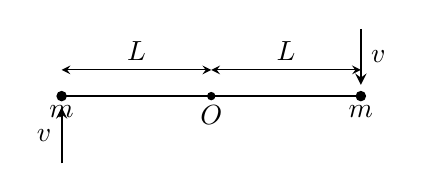
\begin{tikzpicture}[scale=0.95,>=stealth]
  \draw[thick] (-2.0,0) -- (2.0,0);
  \fill (0,0) circle (1.6pt) node[below] {\(O\)};
  \fill (-2.0,0) circle (2pt) node[below] {\(m\)};
  \fill (2.0,0) circle (2pt) node[below] {\(m\)};
  \draw[->,thick] (-2.0,-0.9) -- (-2.0,-0.15) node[midway,left] {\(v\)};
  \draw[->,thick] (2.0,0.9) -- (2.0,0.15) node[midway,right] {\(v\)};
  \draw[<->] (0,0.35) -- (2.0,0.35) node[midway,above] {\(L\)};
  \draw[<->] (-2.0,0.35) -- (0,0.35) node[midway,above] {\(L\)};
\end{tikzpicture}
\end{center}
\end{exercise}

\begin{solution}
\textbf{起手判断/模型：} 碰撞时间很短，转轴支持力对轴的力矩为零，阻力矩在碰撞瞬间可忽略，所以先对 \(O\) 轴用角动量守恒。碰后受恒定阻力矩停转时，角动量随时间线性减少。

\textbf{碰撞瞬间：} 两个小球对 \(O\) 轴的初始角动量方向相同，大小为
\[
L_0=mvL+mvL=2mvL.
\]
细杆绕中点的转动惯量为
\[
J_{\text{杆}}=\frac{1}{12}m(2L)^2=\frac13mL^2.
\]
两个小球粘在两端后贡献
\[
J_{\text{球}}=2mL^2.
\]
因此
\[
J=\frac13mL^2+2mL^2=\frac73mL^2.
\]
角动量守恒给出
\[
2mvL=J\omega_0
\implies
\omega_0=\frac{2mvL}{\frac73mL^2}
=\frac{6v}{7L}.
\]

\textbf{停转阶段：} 恒定阻力矩使角动量从 \(J\omega_0\) 减到零：
\[
Mt=J\omega_0.
\]
而 \(J\omega_0\) 正好等于碰撞后的初始角动量 \(2mvL\)，故
\[
t=\frac{2mvL}{M}.
\]

\textbf{结论：}
\[
\boxed{\omega_0=\frac{6v}{7L}},\qquad
\boxed{t=\frac{2mvL}{M}}.
\]

\textbf{物理检查/易错点：} 杆长是 \(2L\)，绕中心的转动惯量才是 \(\frac13mL^2\)，不要误写成 \(\frac1{12}mL^2\)。停转时间也可由 \(M=J\alpha\) 与 \(t=\omega_0/\alpha\) 得到，本质上仍是角动量定理。
\end{solution}

\begin{exercise}[]
质量为 \(m\)、长度为 \(\ell\) 的均匀细杆，求它绕中心且垂直于杆的轴，以及绕一端且垂直于杆的轴的转动惯量。
\end{exercise}

\begin{solution}
\textbf{起手判断/模型：} 这题看似要算两个转动惯量，其实真正的起手判断是：第二个转轴是不是和第一个\textbf{平行}。一旦认出“绕中点”和“绕端点”的两条轴互相平行，就该先调平行轴定理，而不是把积分从头做两遍。

\textbf{主方程与化简：} 对绕端点的情形，两轴距离为 \(d=\ell/2\)，于是
\[
\begin{aligned}
J_C&=\frac{1}{12}m\ell^2,\\
J_O&=J_C+md^2
=\frac{1}{12}m\ell^2+m\left(\frac{\ell}{2}\right)^2
=\left(\frac{1}{12}+\frac{1}{4}\right)m\ell^2
=\frac{1}{3}m\ell^2.
\end{aligned}
\]

\textbf{结论：} \(J_C=\frac{1}{12}m\ell^2,\ J_O=\frac{1}{3}m\ell^2\)。

\textbf{物理检查/易错点：} 绕端点转时，质量分布平均离轴更远，所以 \(J_O>J_C\) 是必须满足的；结果 \(\frac13 m\ell^2>\frac1{12}m\ell^2\)，方向正确。最容易错的是没先判断“轴是否平行”，或者把轴距误写成 \(\ell\) 而不是 \(\ell/2\)。
\end{solution}

\begin{exercise}[]
若外力矩可以忽略，花样滑冰运动员把转动惯量从 \(J_1\) 缩小到 \(J_2\)，角速度会怎样变化？
\end{exercise}

\begin{solution}
\textbf{起手判断/模型：} 题目主动告诉你“外力矩可以忽略”，这就是角动量守恒题的明确信号。此时不能先盯角速度本身，而要先看守恒量。

\textbf{主方程与化简：}
\[
L=J\omega,\qquad
J_1\omega_1=J_2\omega_2
\implies
\omega_2=\frac{J_1}{J_2}\omega_1.
\]

\textbf{结论：} 转动惯量减小时，角速度会增大；若 \(J_2<J_1\)，则 \(\frac{J_1}{J_2}>1\implies \omega_2>\omega_1\)，具体关系为 \(\omega_2=\frac{J_1}{J_2}\omega_1\)。

\textbf{物理检查/易错点：} 这里守恒的是角动量，不是角速度，所以 \(J\) 变小时 \(\omega\) 必须反向补偿。若外力矩不能忽略，或者研究的不是同一转轴，这个结论就不能直接套。
\end{solution}

\part{振动与波动}

\chapter{机械振动}

\begin{skill}[第5章冲刺总手册]\label{sk:phys-ch05-overview}
\textbf{【这章先解决什么题】} 这章处理“来回振”的题：弹簧振子、单摆、复摆、扭摆、初相、周期、能量、阻尼、受迫和共振。真正的核心只有一句话：先把回复作用写成“与位移成正比”。

\textbf{【拿题先认什么信号】} 题面若出现“平衡位置附近小振动、回复力、周期、频率、振幅、初相、共振”，就先判断能否近似为简谐振动；若题目说“小角度单摆”，等价信号就是 \(\sin\theta\approx\theta\) 后得到线性方程。

\textbf{【第一条方程先写什么】}
\[
m\ddot x+kx=0
\quad \text{或} \quad
\ddot x+\omega^2x=0.
\]
对转动振子则把 \(x\) 换成 \(\theta\)，把 \(m\) 换成转动惯量 \(J\)。

\textbf{【必背公式块】}
\[
\begin{aligned}
x&=A\cos(\omega t+\varphi_0),\\
v&=-\omega A\sin(\omega t+\varphi_0),\qquad
a=-\omega^2x,\\
T&=\frac{2\pi}{\omega},\qquad
f=\frac{1}{T},\\
\omega_{\text{弹簧}}&=\sqrt{\frac{k}{m}},\qquad
\omega_{\text{小角单摆}}=\sqrt{\frac{g}{l}},\\
E&=\frac12 kA^2=\frac12 m\omega^2A^2
=\frac12 kx^2+\frac12 mv^2.
\end{aligned}
\]
若有弱阻尼，可记 \(x\propto e^{-\beta t}\cos(\omega_d t+\varphi_0)\)；若问共振，先认外驱频率 \(\Omega\) 是否接近固有频率 \(\omega_0\)。

\textbf{【做题流程】} 先找平衡位置，并把位移从平衡位置量起；再写回复力或回复力矩，确认它是否正比于位移；由此读出 \(\omega\)；若题目给 \(x_0,v_0\)，就联立标准式定 \(A,\varphi_0\)；若题目给最大位移或过平衡位置速度，直接用能量关系更快。

\textbf{【最容易误判】} 原点没放在平衡位置；只凭 \(x_0=0\) 就草率给初相，忘了还要看速度方向；把“周期振动”误当“简谐振动”；单摆角度不小却还套小角公式。

\textbf{【最后怎样验证】} 看 \(a\) 是否始终指向平衡位置；看 \(x=0\) 时速率是否最大；看量纲里 \(\omega\) 是否为 \(\si{rad/s}\)；若共振题算出阻尼越大振幅越大，说明方向判反了。
\end{skill}

\chapterroadmap
{研究物体在平衡位置附近为什么会来回振动，并把不同模型统一到一条“回复作用”主线上。}
{已经会用受力分析和能量守恒处理基础力学问题，也知道导数可以描述位置和速度怎样变化。}
{新增简谐振动判据、动力学方程与运动学方程、单摆/复摆/扭摆、振动能量、振动合成、拍频、阻尼振动、受迫振动和共振。}

\bridge{这一章最关键的动作，不是记更多三角函数，而是把“图景”和“方程”真正连起来。读这一章时，始终先问三件事：平衡位置在哪里；偏离后谁在把它拉回去；这种拉回去的作用是否与位移成正比。只要这三步不乱，后面的方程、相位、能量和合成都会顺起来。}

\section{先找平衡位置，再谈振动}

自学振动最容易犯的第一个错误，是把任何“来回运动”都直接叫成简谐振动。其实振动先要有平衡位置：如果物体待在那里时合力为零，稍微偏离后又会受到把它拉回去的作用，才可能形成稳定振动。简谐振动只是振动里最重要、也最理想的一类，因为它的回复作用恰好与位移成正比。

所以看到振动题时，第一步往往不是写三角函数，而是先问：
\begin{itemize}
  \item 平衡位置在哪里；
  \item 位移 \(x\) 或角位移 \(\theta,\varphi\) 是从哪里量起的；
  \item 偏离平衡位置后，回复力或回复力矩是否近似与位移成正比。
\end{itemize}

\begin{note}
很多题里最关键的一步，就是把坐标原点从“自然长度位置”或“最低点”改成“平衡位置”。一旦原点选对，重力等恒定外力常会被平衡条件抵消，方程立刻变得简单。
\end{note}

\section{什么是机械振动}

如果一个物体在平衡位置附近作往复运动，并且这种运动具有周期性，就称为机械振动。弹簧振子、单摆、音叉、钟摆都属于这一类问题。

但这里要先分清两句话：
\begin{itemize}
  \item \textbf{机械振动}强调的是“在平衡位置附近来回运动”；
  \item \textbf{简谐振动}强调的是“这种往复运动还满足一条特别整齐的数学规律”。
\end{itemize}

所以，周期振动不一定是简谐振动；简谐振动只是周期振动里最规则、最容易完整求解的一种。

\section{什么才叫简谐振动}

这一节要解决的问题是：什么样的往复运动，才能放心地套用整套简谐公式？

真正该先认出来的，不是“它长得像不像余弦曲线”，而是偏离平衡位置后，系统有没有一种特别整齐的回复规律。若回复力总能写成“大小正比于位移、方向永远指回平衡位置”，那么运动方程就会变成线性的二阶常系数方程；而线性方程之所以重要，正是因为它的解会自然长成正弦或余弦形式。也就是说，\textbf{简谐振动不是先有三角函数，再去找物理解释；而是先有线性回复，再从方程里长出三角函数。}

\begin{definition}[简谐振动]\label{def:simple-harmonic-motion}
若振动物体的位移可以表示为 \(x=A\cos(\omega t+\varphi_0)\)，则称该振动为\textbf{简谐振动}。
\end{definition}

其中 \(A\) 是振幅，\(\omega\) 是角频率，\(\varphi=\omega t+\varphi_0\) 是相位，\(\varphi_0\) 是初相。

课件里常把“证明一个运动是简谐振动”的入口整理成四条判据。它们看起来像四句话，其实说的是同一件事：
\begin{enumerate}
  \item 合外力满足 \(F=-kx\)，也就是回复力与位移成正比、方向相反；
  \item 势能可写成二次型 \(U=\frac{1}{2}kx^2\)，并且系统机械能守恒；
  \item 动力学方程可写成 \(\dv[2]{x}{t}+\omega^2x=0\)；
  \item 运动学方程可写成 \(x=A\cos(\omega t+\varphi_0)\)。
\end{enumerate}

\begin{note}
最容易混淆的点是：\textbf{有周期}并不自动推出\textbf{是简谐振动}。例如大摆角单摆仍然会周期性摆动，但因为回复力不再严格正比于位移，所以不能直接算作简谐振动。
\end{note}

\section{动力学方程与运动学方程}

这一节要解决的问题是：简谐振动的方程到底有几种，它们之间是什么关系？

简谐振动最稳的主线就是下面这条链：
\begin{align*}
F=-kx &\implies m\dv[2]{x}{t}=-kx\\
      &\implies \dv[2]{x}{t}+\omega^2x=0\\
      &\implies x=A\cos(\omega t+\varphi_0).
\end{align*}
其中 \(\omega^2=\frac{k}{m}\)。

\begin{note}
从 \(\dv[2]{x}{t}+\omega^2x=0\) 走到 \(x=A\cos(\omega t+\varphi_0)\)，中间其实只隔着一层你已经会的常系数二阶微分方程：它的通解先写成
\[
x=C_1\cos\omega t+C_2\sin\omega t,
\]
再把两个常数改写成振幅 \(A\) 和初相 \(\varphi_0\)，就压成了最常用的
\[
x=A\cos(\omega t+\varphi_0).
\]
把它代回去检查，就能直接验证它确实满足 \(x''=-\omega^2x\)。

为什么这就是\textbf{全部}的解？二阶ODE的通解恰好包含两个独立常数（对应两个初始条件：初始位置和初始速度）。\(\cos\omega t\) 和 \(\sin\omega t\) 是两个线性无关的解，它们的任意线性组合 \(C_1\cos\omega t+C_2\sin\omega t\) 就穷尽了所有可能的解。所以一旦给定 \(x(0)\) 和 \(\dot{x}(0)\)，\(A\) 和 \(\varphi_0\) 就被唯一确定，不存在其他形式的解。
\end{note}

这里面有两个不同层次的方程：
\begin{itemize}
  \item \textbf{动力学方程}讨论“力怎样决定运动”，典型形式是
  \[
  m\dv[2]{x}{t}+kx=0
  \quad \text{或} \quad
  \dv[2]{x}{t}+\omega^2x=0;
  \]
  \item \textbf{运动学方程}讨论“位置怎样随时间变化”，典型形式是 \(x=A\cos(\omega t+\varphi_0)\)。
\end{itemize}

\bridge{这一章更强调先写动力学方程，再回到位移公式。因为振动模型真正的物理根子，不是三角函数本身，而是“回复作用和位移成正比”这件事。}

把位移方程求两次导数，就会得到 \(a=\dv[2]{x}{t}=-\omega^2x\)。
这条式子特别重要，因为它把“受力观点”和“位移观点”接上了：一旦你能证明加速度总指向平衡位置，且大小与位移成正比，简谐振动的整套结构就立起来了。

\begin{exercise}[用平衡位置证明竖直弹簧振子作简谐振动]
一轻弹簧上端固定，下端挂一重物。静止时弹簧伸长 \(l=9.8\ \text{cm}\)。现给物体一个向下的瞬时冲击，使它在 \(t=0\) 时通过平衡位置并具有向下速度 \(v_0=1\ \text{m/s}\)。证明物体作简谐振动，并写出振动方程。
\end{exercise}

\begin{solution}
\textbf{起手判断/模型：} 这题真正的第一步不是急着定初相，而是先把位移从\textbf{平衡位置}起量。因为只要原点选在平衡位置，重力和静伸长对应的那一部分弹力就会先互相抵消，方程才会直接落回简谐振动标准型。

\textbf{主方程：} 取平衡位置为原点 \(O\)，向下为 \(x\) 轴正方向。静止时有
\[
kl=mg,\qquad mg-k(l+x)=m\dv[2]{x}{t}.
\]
\begin{note}
这一步真正关键的是把弹力拆成两部分看：\(k(l+x)=kl+kx\)。其中 \(kl\) 正好对应弹簧的\textbf{静伸长}，它只负责在平衡时抵消重力；真正让物体围绕平衡位置来回振动的，是额外那一段回复力 \(kx\)。所以把原点放在平衡位置后，\(mg\) 和 \(kl\) 会先抵消，只剩 \(x\) 这一项进入振动方程。
\end{note}

\textbf{分步代入或化简：} 用平衡条件 \(kl=mg\) 消去常量项，得到
\[
m\dv[2]{x}{t}+kx=0
\implies \dv[2]{x}{t}+\frac{k}{m}x=0
\implies \omega^2=\frac{k}{m}=\frac{g}{l}=\frac{9.8}{0.098}=100
\implies \omega=10\ \si{s^{-1}}.
\]
\begin{note}
这里的 \(\omega^2=\frac{k}{m}=\frac{g}{l}\) 只对这道“竖直弹簧、已知静伸长 \(l\)”的题成立，因为它额外用了平衡条件 \(kl=mg\)。离开这个背景时，最该先记住的通式仍是 \(\omega^2=k/m\)，不要把 \(g/l\) 误当成所有简谐振动都通用的结论。
\end{note}
振动方程先写成
\[
x=A\cos(10t+\varphi_0),\qquad
x(0)=0 \implies A\cos\varphi_0=0 \implies \varphi_0=\pm\frac{\pi}{2},\qquad
v(0)=-10A\sin\varphi_0=1.
\]
由于题目给的是\textbf{向下通过平衡位置}，而我们取向下为正，所以 \(v(0)>0\)。要使上式右端为正，必须有 \(\sin\varphi_0<0\)，因此可继续压成
\[
\varphi_0=-\frac{\pi}{2},\qquad
A=\frac{1}{10}=0.10\ \si{m}
\implies
x=0.10\cos\left(10t-\frac{\pi}{2}\right)=0.10\sin(10t).
\]

\textbf{结论：} 振动方程可写成上式。

\textbf{物理检查/易错点：} 质点在 \(t=0\) 通过平衡位置，所以那一刻速率应为最大值，代入 \(v_{\max}=\omega A\) 也有 \(A=v_{\max}/\omega=1/10=\SI{0.10}{m}\)，与上面一致。最容易错的地方有两处：一是原点没放在平衡位置，导致方程里残留常量项；二是只由 \(x(0)=0\) 就草率取 \(\varphi_0=\pi/2\)，忘了还要用速度方向判象限。
\end{solution}

\section{速度与加速度}

从位移方程
\[
\begin{aligned}
x&=A\cos(\omega t+\varphi_0),\\
v&=\dv{x}{t}=-A\omega\sin(\omega t+\varphi_0),\\
a&=\dv{v}{t}=-A\omega^2\cos(\omega t+\varphi_0)
\implies a=-\omega^2x.
\end{aligned}
\]

这说明简谐振动中的速度、加速度也都是周期变化的，而且加速度总是指向平衡位置。进一步可得 \(v_{\max}=\omega A,\ a_{\max}=\omega^2A\)。

\begin{note}
只要把平衡位置、端点和平常中间位置分清，很多量就不会混：
\begin{itemize}
  \item 在平衡位置 \(x=0\) 处，回复力和加速度为零，但速度最大；
  \item 在端点 \(x=\pm A\) 处，速度为零，但加速度大小最大；
  \item 在中间位置，位移、速度、加速度一般都不为零。
\end{itemize}
\end{note}

\section{怎样读懂相位}

这一节要解决的问题是：相位到底在描述什么，为什么它比“位置”更能代表振动状态？

同一简谐振动里，位移、速度、加速度都由同一个相位 \(\varphi=\omega t+\varphi_0\) 控制。相位相同，说明“振动状态”相同；相位不同，说明它们虽然可能位移一样，但运动方向、受力状态未必相同。

例如，当 \(x=0\) 时，质点可能正向右穿过平衡位置，也可能正向左穿过平衡位置。单看位移分不出来，但结合相位或者速度符号就能区分。也就是说，位移只告诉你“现在在哪里”，相位则告诉你“现在振到了哪一步”。

\begin{remark}
相位很容易被误当成“又一个角度定义”。更直观的理解是：相位就是振动进程条。它不只是记录位置，还同时编码了“接下来往哪边动”。
\end{remark}

\section{旋转矢量法：把相位画出来}

\begin{definition}[旋转矢量法]
把长度为 \(A\) 的矢量放在平面内，让它以角速度 \(\omega\) 匀速逆时针转动。若 \(t=0\) 时它与 \(x\) 轴夹角为 \(\varphi_0\)，则时刻 \(t\) 的夹角为
\[
\theta=\omega t+\varphi_0
\implies
x=A\cos\theta=A\cos(\omega t+\varphi_0),
\]
这正是简谐振动方程。
\end{definition}

\bridge{旋转矢量法最有用的地方，不是“多了一张图”，而是把抽象的相位变成了真正可以在平面上看见的角位置。后面讲振动合成和拍频时，这个方法会再次出现。}

\begin{note}
只知道初始位置 \(x_0\)，通常只能确定旋转矢量在 \(x\) 轴上的投影，因此会有两个关于 \(x\) 轴对称的可能位置；再结合初始速度方向，才能判断它在上半平面还是下半平面，从而唯一确定初相。
\end{note}

\section{由初始位置和初始速度确定初相}

\begin{note}
\textbf{先看什么信号：} 题目若同时给 \(x_0\) 和“向哪边运动”，八成是在让你判初相所在象限；\textbf{这条公式在控制什么：} \(x_0\) 决定 \(\cos\varphi_0\)，\(v_0\) 决定 \(-\sin\varphi_0\) 的符号；\textbf{怎样最快记住：} 位置先定“横坐标”，速度再定“上半平面还是下半平面”；\textbf{最容易错：} 由 \(\cos\varphi_0=x_0/A\) 只取一个角，忘了余弦通常对应两个关于 \(x\) 轴对称的候选象限。
\end{note}

若振动方程写成
\[
\begin{aligned}
x&=A\cos(\omega t+\varphi_0) \\
\implies\quad x_0&=A\cos\varphi_0,\qquad v_0=-A\omega\sin\varphi_0.
\end{aligned}
\]
因此定初相的标准步骤是：
\begin{enumerate}
  \item 先由 \(\cos\varphi_0=x_0/A\) 找到两个可能角；
  \item 再用 \(v_0\) 的正负判断 \(\sin\varphi_0\) 的符号，选出正确象限；
  \item 最后再检查该初相是否与题目给出的初始运动方向一致。
\end{enumerate}

\begin{exercise}[由位置和速度确定初相]
某简谐振动的振幅为 \(A\)，角频率为 \(\omega\)。已知 \(t=0\) 时 \(x_0=A/2\)，且质点正沿负方向运动。求初相 \(\varphi_0\)。
\end{exercise}

\begin{solution}
\[
\begin{aligned}
x_0=A\cos\varphi_0=\frac{A}{2}
&\implies \cos\varphi_0=\frac{1}{2}
\implies \varphi_0=\frac{\pi}{3}\quad \text{或}\quad \frac{5\pi}{3},\\
v_0=-A\omega\sin\varphi_0<0
&\implies \sin\varphi_0>0
\implies \varphi_0=\frac{\pi}{3}.
\end{aligned}
\]

所以这道题的标准做法是：\textbf{先用位置确定余弦，再用速度方向确定正弦的符号。}
\end{solution}

\section{周期和频率}

这一节真正要先读进去的，不是三个符号之间的代换，而是“同一个系统按固定节奏重复自己”这件事该怎样定量描述。若你盯住某个质点看，它每隔一段固定时间就回到完全相同的振动状态，这个时间尺度就是周期；若你改成问“每秒重复多少次”，那就是频率；而角频率 \(\omega\) 只是把“重复得多快”改写成圆周运动里更顺手的角量语言。

简谐振动的周期、频率与角频率的关系为
\[
T=\frac{2\pi}{\omega},\qquad f=\frac{1}{T},\qquad \omega=2\pi f.
\]

\begin{note}
理想简谐振动里，周期是由系统本身决定的“固有节奏”。对于理想弹簧振子、小角度单摆和扭摆，周期都不直接依赖于初始相位；在理想模型下，周期也不随振幅改变。
\end{note}

\section{弹簧振子}

弹簧振子是最基本的简谐振动模型。设质量为 \(m\) 的小球连在劲度系数为 \(k\) 的轻弹簧上，在光滑水平面上运动。由胡克定律和牛顿第二定律，
\[
\begin{aligned}
-kx&=m\dv[2]{x}{t}
\implies m\dv[2]{x}{t}+kx=0 \\
\implies\quad
\omega=\sqrt{\frac{k}{m}},\qquad
T=2\pi\sqrt{\frac{m}{k}}.
\end{aligned}
\]

\begin{remark}
对竖直弹簧振子，只要把位移从\textbf{平衡位置}开始量，最后得到的方程仍然是同一形式。所以水平弹簧振子和竖直弹簧振子，看起来受力不同，真正的振动核心却是一样的。
\end{remark}

\begin{exercise}[水平弹簧振子为什么一写出来就是余弦]
质量为 \(m=\SI{20}{g}\) 的小球连在劲度系数 \(k=\SI{0.72}{N/m}\) 的轻弹簧上，在光滑水平面上运动。若初始时刻小球位于 \(x_0=\SI{5.0}{cm}\) 处并由静止释放，求振动方程。
\end{exercise}

\begin{solution}
\textbf{起手判断/模型：} 题目已经给出 \(m,k\) 和初始位置、初始速度，所以先认这是标准\textbf{水平弹簧振子}。第一条方程不是直接猜余弦，而是先从
\[
m\ddot x+kx=0
\]
写出角频率，再用初始条件定振幅和初相。

\textbf{主方程：}
\[
\omega=\sqrt{\frac{k}{m}},\qquad
x=A\cos(\omega t+\varphi_0).
\]

\textbf{分步代入或化简：} 先算角频率：
\[
\omega=\sqrt{\frac{0.72}{0.020}}=\sqrt{36}=\SI{6}{rad/s}.
\]
又因
\[
x(0)=A\cos\varphi_0=\SI{0.050}{m},\qquad
v(0)=-A\omega\sin\varphi_0=0.
\]
第二式说明 \(\sin\varphi_0=0\)，而初始时位移为正且恰由静止释放，所以应取
\[
\varphi_0=0,\qquad A=\SI{0.050}{m}.
\]

\textbf{结论：}
\[
x=0.050\cos(6t)\ \si{m}.
\]

\textbf{物理检查/易错点：} 由正端点静止释放，所以 \(t=0\) 一定在最大位移处，写成余弦比写成正弦更自然。最容易错的是只凭 \(v_0=0\) 就写 \(\varphi_0=0\)，却不再用 \(x_0>0\) 检查符号。
\end{solution}

\section{小角度单摆}

这一节要解决的问题是：为什么单摆只在小角度时才近似成为简谐振动？

设摆长为 \(\ell\)，摆球质量为 \(m\)，摆角 \(\theta\) 从平衡位置开始计。摆球受到的切向回复力为
\[
\begin{aligned}
F_{\tau}&=-mg\sin\theta,\qquad
a_{\tau}=\dv[2]{s}{t}=\ell\dv[2]{\theta}{t} \\
\implies\quad
m\ell\dv[2]{\theta}{t}&=-mg\sin\theta
\implies
\dv[2]{\theta}{t}+\frac{g}{\ell}\sin\theta=0.
\end{aligned}
\]

这一步还不是简谐振动，因为方程里出现的是 \(\sin\theta\)，而不是直接正比于 \(\theta\)。只有在摆角较小时，才能采用近似并压成
\[
\sin\theta\approx \theta
\implies
\dv[2]{\theta}{t}+\frac{g}{\ell}\theta=0
\implies
\omega=\sqrt{\frac{g}{\ell}},\qquad
T=2\pi\sqrt{\frac{\ell}{g}}.
\]
这时单摆才近似作简谐振动。

\bridge{单摆成为简谐振动的关键，不是“它会来回摆”，而是“小角度时 \(\sin\theta\) 可以用 \(\theta\) 代替”。也就是说，真正把它拉回到简谐模型里的，是这个近似。}

\begin{note}
这条周期公式最容易误用。它只适用于小摆角近似；摆角一大，周期会比这个公式给出的结果更长，不能再直接套用。
\end{note}

\section{复摆}

这一节要解决的问题是：如果摆动的不再是质点，而是整个刚体，简谐模型还怎样保留？

\textbf{先别急着背周期公式。} 单摆之所以能来回摆，是因为一旦偏离平衡位置，重力就会对悬点产生一个想把它拉回去的回复力矩。复摆里转动的虽然不再是质点，而是整个刚体，但这条主线完全没变：重力仍然负责提供回复力矩，只是“有多难被转起来”已经不能只看质量 \(m\)，而必须看绕支点轴的转动惯量 \(J_O\)。

\textbf{复摆}是指在重力作用下，能绕某固定水平轴作微小摆动的刚体。设刚体质量为 \(m\)，支点到质心的距离为 \(d\)，绕支点轴的转动惯量为 \(J_O\)，偏角记为 \(\theta\)。当刚体偏离平衡位置后，重力 \(mg\) 仍作用在质心上；相对支点看，它的力臂是 \(d\sin\theta\)。若约定使 \(\theta\) 增大的方向为正，则重力矩总是企图把偏角压回去，因此关于支点的回复力矩自然写成
\[
\begin{aligned}
M_O&=-mgd\sin\theta \\
\sin\theta\approx \theta\ &\implies\ M_O\approx -mgd\,\theta \\
J_O\dv[2]{\theta}{t}&=M_O
\implies J_O\dv[2]{\theta}{t}+mgd\,\theta=0 \\
\implies\quad
\omega=\sqrt{\frac{mgd}{J_O}},\qquad
T=2\pi\sqrt{\frac{J_O}{mgd}}.
\end{aligned}
\]

\begin{note}
\textbf{先记结构再记结果：} 复摆真正的骨架是“回复力矩 = 转动惯性项”，也就是 \(M_O=J_O\ddot{\theta}\)；只有把 \(\sin\theta\) 在线性近似下换成 \(\theta\)，它才会退化成熟悉的简谐振动方程。最容易写错的不是周期，而是忘了 \(M_O=-mgd\sin\theta\) 里的负号正是在表达“力矩总要把偏角往回扳”。
\end{note}

\begin{remark}
若把复摆的等效摆长定义为 \(\ell_{\text{eq}}=\frac{J_O}{md}\)，则复摆周期也可写成
\[
T=2\pi\sqrt{\frac{\ell_{\text{eq}}}{g}}.
\]
这说明复摆并不是“完全陌生的新摆”，而是单摆思路在刚体上的推广。
\end{remark}

\section{扭摆}

这一节要解决的问题是：如果物体不是左右平移，也不是前后摆动，而是绕轴轻微扭转，它还能不能作简谐振动？

\textbf{这里的回复作用不再来自重力，而来自金属丝本身的弹性。} 若把圆盘顺时针拧开一点，细丝内部就会出现一个反向的恢复力矩，想把圆盘扳回原来的取向。因此扭摆最先该写的不是周期，而是“角位移版胡克定律”：偏得越多，扭回去的力矩越大，而且方向总与扭转角相反。

\textbf{扭摆}的典型模型是圆盘悬挂在金属丝下端，绕竖直轴作微小扭转。设扭转角为 \(\varphi\)，金属丝的扭转系数为 \(D\)，圆盘绕转轴的转动惯量为 \(J\)。当扭转角不大时，回复力矩满足
\[
M=-D\varphi,\qquad
J\dv[2]{\varphi}{t}=M
\implies
J\dv[2]{\varphi}{t}+D\varphi=0
\implies
\omega=\sqrt{\frac{D}{J}},\qquad
T=2\pi\sqrt{\frac{J}{D}}.
\]

\bridge{扭摆本质上就是“角位移版弹簧振子”：平移里是 \(F=-kx\)，扭转里是 \(M=-D\varphi\)；平移里是质量 \(m\)，扭转里是转动惯量 \(J\)。只要把这组对应关系抓住，扭摆就不会显得陌生。}

\begin{note}
\textbf{最快的记忆钩子就是三组平行对应：} \(x\leftrightarrow\varphi\)，\(k\leftrightarrow D\)，\(m\leftrightarrow J\)。所以一看到扭摆，就别先找重力，而要先找“角位移版弹簧振子”的回复规律。这里的周期也不由重力决定，而由“刚体有多难扭动”和“金属丝有多想把它扭回去”共同决定。
\end{note}

\section{振动能量}

这一节要解决的问题是：为什么一个看起来只是“来回摆动”的振子，也能像抛体或斜面问题那样谈能量守恒？

以弹簧振子为例，先别急着把 \(E_k=\frac12 mv^2\)、\(E_p=\frac12 kx^2\) 当成现成结论背下来。真正该先想的是：同一个振子经过平衡位置时，明明 \(x=0\) 却跑得最快；到达端点时，明明 \(v=0\) 却又能自己掉头回来。这说明系统里至少有两种不同的“储能方式”：一部分跟\textbf{质点此刻动得多快}有关，另一部分跟\textbf{弹簧此刻被拉伸或压缩得多厉害}有关。

前者就是平动里已经认识过的动能：
\[
E_k=\frac12 mv^2.
\]
后者则要从“把弹簧从平衡位置缓慢拉到 \(x\) 时，外界一共做了多少功”自然长出来。关键先别急着看结果，而要先看力学图景：弹簧的回复力不是常量，而是随位移线性增大，越拉越费力，所以储存起来的势能不可能是“力乘位移”那样的一次量，而必须是对这股\textbf{逐步增大的阻力}做功的累计。这样一来，势能就只能从积分里长出来。因为回复力满足 \(F_x=-kx\)，取平衡位置为零势能点，就有
\[
E_p=-\int_0^x F_x\,\dd x'
=\int_0^x kx'\,\dd x'
=\frac12 kx^2.
\]

接下来再看任一时刻的能量分配。这里也最好先有图景再读公式：位移控制的是“弹簧此刻被拉了多少”，所以势能会跟 \(x^2\) 走；速度控制的是“质点此刻冲得多快”，所以动能会跟 \(v^2\) 走。对简谐振动来说，\(x\) 与 \(v\) 本来就相差四分之一个周期，于是能量分配自然会拆成一边随 \(\cos^2\) 变、一边随 \(\sin^2\) 变。把这层图景先放在脑子里，再看下面这组式子就不会停顿：
\[
\begin{aligned}
x&=A\cos(\omega t+\varphi_0),\qquad
v=-A\omega\sin(\omega t+\varphi_0),\\
E_k&=\frac12 mA^2\omega^2\sin^2(\omega t+\varphi_0),\qquad
E_p=\frac12 kA^2\cos^2(\omega t+\varphi_0),\\
x=\pm A,\ v=0
&\implies E=\frac12 kA^2,\qquad
x=0,\ v=\omega A\implies E=\frac12 m\omega^2A^2,\\
&\therefore E=E_k+E_p=\frac12 kA^2=\frac12 m\omega^2A^2.
\end{aligned}
\]
这里最自然的总能量求法，其实不是每次都把三角函数硬代到底，而是先抓最容易的两个位置：\textbf{端点处全是势能，平衡位置处全是动能。} 同时别忘了这两种写法之所以真是同一个总能量，还偷偷用了简谐振动的核心关系 \(\omega^2=k/m\)。正因为 \(m\omega^2=k\)，\(\frac12 m\omega^2A^2\) 和 \(\frac12 kA^2\) 才是同一个量。

\bridge{这个结果很值得慢慢体会。简谐振动虽然速度、位移、受力都在变，但系统总能量不变，只是在动能和势能之间来回交换。换句话说，振子不是“忽然快、忽然慢”而已，它一直在做能量形式的交换。}

于是可以顺着位置来理解能量分配：
\begin{itemize}
  \item 当质点经过平衡位置时，\(x=0\)，势能最小；此时速度最大，因此动能最大；
  \item 当质点到达端点时，\(v=0\)，动能为零；但弹簧形变量最大，因此势能最大；
  \item 在中间位置时，动能和势能都不为零，它们的和始终等于同一个总能量。
\end{itemize}

这也解释了为什么总能量和振幅平方成正比：振幅越大，端点处弹簧被拉得越长、压得越深，系统能储存的最大势能就越大，因此整次振动携带的总能量也越大。

\begin{exercise}[由位移判断能量分配]
某弹簧振子振幅为 \(A\)。当质点位于 \(x=A/2\) 处时，求动能和势能各占总机械能的多少。
\end{exercise}

\begin{solution}
总机械能与当前位置势能可并成
\[
E=\frac{1}{2}kA^2,\qquad
E_p=\frac{1}{2}k\left(\frac{A}{2}\right)^2=\frac{1}{8}kA^2=\frac{1}{4}E
\implies
E_k=E-E_p=\frac{3}{4}E.
\]

所以在 \(x=A/2\) 这个位置，势能占总能量的 \(1/4\)，动能占总能量的 \(3/4\)。这种题最稳的入口通常不是先求速度，而是先用能量表达式直接分配。
\end{solution}

\begin{remark}
如果把振幅变成原来的 2 倍，总机械能会变成原来的 4 倍。这就是“振幅平方决定能量量级”的最直接体现，也是后面理解拍频强弱变化和波动能量的共同基础。
\end{remark}

\begin{exercise}[已知 \(m,A,a_{\max}\) 时怎样反求周期和能量]
一简谐振子质量 \(m=\SI{0.10}{kg}\)，振幅 \(A=\SI{1.0e-2}{m}\)，最大加速度 \(a_{\max}=\SI{4.0}{m/s^2}\)。求其周期、经过平衡位置时的动能、总机械能，并求在什么位置有 \(E_k=E_p\)。
\end{exercise}

\begin{solution}
\textbf{起手判断/模型：} 题目给的是 \(A\) 和 \(a_{\max}\)，所以第一步先别找速度，而应先用简谐振动里
\[
a=-\omega^2 x
\]
这一层关系。因为最大加速度一定出现在端点 \(x=\pm A\)，这会直接给出 \(\omega\)。

\textbf{主方程：}
\[
a_{\max}=\omega^2 A,\qquad
T=\frac{2\pi}{\omega},\qquad
E=\frac12 kA^2=\frac12 m\omega^2A^2.
\]

\textbf{分步代入或化简：} 先由最大加速度求角频率：
\[
\omega^2=\frac{a_{\max}}{A}=\frac{4.0}{1.0\times 10^{-2}}=400
\implies
\omega=\SI{20}{rad/s}.
\]
于是
\[
T=\frac{2\pi}{20}=\frac{\pi}{10}\ \si{s}\approx \SI{0.314}{s}.
\]
经过平衡位置时 \(x=0\)，故势能为零、动能最大，因此
\[
E_k(\text{平衡})=E=\frac12 m\omega^2A^2
=\frac12\times 0.10\times 20^2\times (1.0\times10^{-2})^2
=\SI{2.0e-3}{J}.
\]
所以总机械能也是
\[
E=\SI{2.0e-3}{J}.
\]
若 \(E_k=E_p\)，则二者都等于总能量的一半。由
\[
E_p=\frac12 kx^2,\qquad E=\frac12 kA^2
\]
得
\[
\frac12 kx^2=\frac12 E=\frac14 kA^2
\implies
x^2=\frac{A^2}{2}
\implies
x=\pm \frac{A}{\sqrt2}.
\]

\textbf{结论：}
\[
T\approx \SI{0.314}{s},\qquad
E_k(\text{平衡})=\SI{2.0e-3}{J},\qquad
E=\SI{2.0e-3}{J},\qquad
x=\pm \frac{A}{\sqrt2}.
\]

\textbf{物理检查/易错点：} 最大加速度出现在端点而不是平衡位置，这正是“回复作用在端点最强”的体现。最容易错的是把 \(E_k=E_p\) 误写成 \(x=\pm A/2\)；能量与位移平方成正比，所以应是 \(\pm A/\sqrt2\)。
\end{solution}

\begin{exercise}[斜面弹簧缓慢移动时外力做功怎样算]
轻弹簧一端固定在倾角为 \(\alpha\) 的光滑斜面底端，另一端与质量为 \(m\) 的物体相连。\(O\) 点为弹簧原长处，\(A\) 点为物体平衡位置，\(x_0\) 为弹簧在 \(A\) 点被压缩的长度。若外力将物体由 \(A\) 点沿斜面向上缓慢移动 \(2x_0\) 到 \(B\) 点，求外力所做的功。

\begin{center}

\includegraphics[width=0.22\linewidth]{pdf-exercises/pdf2003-q12-spring-incline.png}
\end{center}
\end{exercise}

\begin{solution}
\textbf{起手判断/模型：} “缓慢移动”说明始末动能可忽略，外力做功等于系统势能的增加。物体从 \(A\) 到 \(B\) 的位移为 \(2x_0\)，弹簧从压缩 \(x_0\) 变为伸长 \(x_0\)，弹性势能前后相同。

\textbf{主方程：}
\[
W_{\text{外}}=\Delta U_g+\Delta U_s.
\]

\textbf{分步代入或化简：} 从 \(A\) 到 \(B\)，沿斜面上升距离为 \(2x_0\)，高度增加
\[
\Delta h=2x_0\sin\alpha.
\]
所以重力势能增加
\[
\Delta U_g=mg\Delta h=2mgx_0\sin\alpha.
\]
弹簧在 \(A\) 点压缩 \(x_0\)，在 \(B\) 点伸长 \(x_0\)，弹性势能均为 \(\frac12kx_0^2\)，故
\[
\Delta U_s=0.
\]

\textbf{结论：}
\[
\boxed{W_{\text{外}}=2mgx_0\sin\alpha}.
\]

\textbf{物理检查/易错点：} 这题最容易把弹簧从压缩到伸长误看成“弹性势能增加”。实际上弹性势能只看形变量大小，压缩 \(x_0\) 和伸长 \(x_0\) 相同。
\end{solution}

\begin{exercise}[2012级期末：恒力推粗糙桌面弹簧物块的最大弹性势能]
如图所示，劲度系数为 \(k\) 的轻弹簧一端固定在墙壁上，另一端连接质量为 \(m\) 的物体。物体在坐标原点 \(O\) 时弹簧为原长，物体与桌面间的滑动摩擦系数为 \(\mu\)。若物体在不变外力 \(F\) 作用下向右移动，求物体到达最远位置时弹簧系统的弹性势能。设 \(F>\mu mg\)。
\end{exercise}

\begin{solution}
\textbf{起手判断/模型：} “最远位置”说明那一瞬间速度为零。初态在 \(O\) 点、弹簧无形变且物体静止；末态速度仍为零，所以外力做功与摩擦耗散后，剩下的能量全部进入弹簧势能。

\textbf{主方程：} 设最远位移为 \(x_m\)。由能量关系
\[
Fx_m-\mu mg\,x_m=\frac12kx_m^2.
\]
除去平凡解 \(x_m=0\)，得
\[
x_m=\frac{2(F-\mu mg)}{k}.
\]

\textbf{弹性势能：}
\[
E_p=\frac12kx_m^2
=\frac12k\left[\frac{2(F-\mu mg)}{k}\right]^2
=\frac{2(F-\mu mg)^2}{k}.
\]

\textbf{结论：}
\[
\boxed{E_p=\frac{2(F-\mu mg)^2}{k}}.
\]

\textbf{物理检查/易错点：} 最大弹性势能不是把力平衡位置 \(x=(F-\mu mg)/k\) 代进去；那只是加速度为零的位置，不是最远点。物体还会凭此前积累的动能继续前进，直到位移达到两倍的平衡位移。
\end{solution}

\begin{exercise}[木板简谐振动时物体不滑的最大振幅]
一物体放在水平木板上，木板以频率 \(\nu=\SI{2}{Hz}\) 沿水平直线作简谐振动。物体与木板间静摩擦系数为 \(\mu_s=0.50\)。求物体不在木板上滑动时木板振动的最大振幅 \(A_{\max}\)。
\end{exercise}

\begin{solution}
\textbf{起手判断/模型：} 物体能跟着木板一起做简谐振动，靠的是静摩擦力提供所需水平加速度。因此最大不滑条件就是“所需最大摩擦力不超过最大静摩擦力”。

\textbf{主方程：}
\[
a_{\max}=\omega^2A,\qquad
f_{\max}=ma_{\max}\le \mu_s mg.
\]

\textbf{分步代入或化简：}
\[
\omega=2\pi\nu,\qquad
m\omega^2A\le \mu_s mg
\implies
A_{\max}=\frac{\mu_s g}{\omega^2}
=\frac{\mu_s g}{4\pi^2\nu^2}.
\]
代入 \(\mu_s=0.50,\ \nu=\SI{2}{Hz}\)，
\[
A_{\max}
=\frac{0.50\times 9.8}{4\pi^2\times 2^2}
\approx \SI{3.1e-2}{m}.
\]

\textbf{结论：}
\[
\boxed{A_{\max}\approx \SI{0.031}{m}}.
\]

\textbf{物理检查/易错点：} 频率越高，同样振幅下所需加速度越大，所以允许振幅应随 \(\nu^{-2}\) 变小。最容易错的是把静摩擦力固定写成 \(\mu_s mg\)，其实它只在临界不滑时达到最大值。
\end{solution}

\begin{exercise}[由振动曲线判断最大速率比]
两简谐振动的位移-时间曲线如图所示，求它们的最大速率之比。

\begin{center}

\includegraphics[width=0.28\linewidth]{pdf-exercises/pdf2003-q17-vibration.png}
\end{center}
\end{exercise}

\begin{solution}
\textbf{起手判断/模型：} 简谐振动最大速率由 \(v_{\max}=A\omega\) 决定，所以读图时要同时读振幅和周期，而不能只看曲线高低。

\textbf{主方程：}
\[
v_{\max}=A\omega=\frac{2\pi A}{T}.
\]

\textbf{读图判断：} 图中 \(x_1\) 的振幅约为 \(\SI{1}{cm}\)，周期约为 \(\SI{2}{s}\)；\(x_2\) 的振幅约为 \(\SI{2}{cm}\)，周期约为 \(\SI{4}{s}\)。因此
\[
\frac{v_{\max,1}}{v_{\max,2}}
=\frac{A_1/T_1}{A_2/T_2}
=\frac{1/2}{2/4}=1.
\]

\textbf{结论：}
\[
\boxed{v_{\max,1}:v_{\max,2}=1:1}.
\]

\textbf{物理检查/易错点：} 第二个振动振幅更大，但周期也更长，两者正好抵消。只看振幅会误判 \(x_2\) 更快。
\end{solution}

\begin{exercise}[2004级期末：由初位移和初速度求振幅与初相]
一简谐振动的表达式为
\[
x=A\cos(3t+\phi).
\]
已知 \(t=0\) 时初位移为 \(\SI{0.04}{m}\)，初速度为 \(\SI{0.09}{m/s}\)。求振幅 \(A\) 和初相 \(\phi\)。
\end{exercise}

\begin{solution}
\textbf{起手判断/模型：} 初位移给出余弦分量，初速度给出正弦分量。先对位移方程求导，再把 \(t=0\) 代入。

\textbf{主方程：}
\[
x(0)=A\cos\phi,\qquad
v(t)=\dv{x}{t}=-3A\sin(3t+\phi).
\]
因此
\[
A\cos\phi=0.04,\qquad
-3A\sin\phi=0.09.
\]

\textbf{分步代入或化简：} 由第二式得
\[
A\sin\phi=-0.03.
\]
所以
\[
A=\sqrt{(A\cos\phi)^2+(A\sin\phi)^2}
=\sqrt{0.04^2+(-0.03)^2}
=\SI{0.05}{m}.
\]
同时
\[
\cos\phi=\frac{0.04}{0.05}=0.8,\qquad
\sin\phi=\frac{-0.03}{0.05}=-0.6.
\]
故 \(\phi\) 位于第四象限，
\[
\phi\approx -36.9^\circ\approx -0.205\pi.
\]

\textbf{结论：}
\[
\boxed{A=\SI{0.05}{m}},\qquad
\boxed{\phi\approx -0.205\pi}.
\]

\textbf{物理检查/易错点：} 只由 \(\tan\phi=-0.75\) 还不能直接定象限，必须同时看 \(\cos\phi>0,\sin\phi<0\)。最容易错的是漏掉速度公式中的负号。
\end{solution}

\begin{exercise}[2005级期末：弹簧振子振幅加倍时总能量怎样变]
一弹簧振子作简谐振动，总能量为 \(E_1\)。若振幅增加为原来的两倍，重物质量增加为原来的四倍，求新的总能量 \(E_2\)。
\end{exercise}

\begin{solution}
\textbf{起手判断/模型：} 弹簧振子的总能量由弹簧劲度系数和振幅决定：
\[
E=\frac12 kA^2.
\]
质量会影响角频率 \(\omega=\sqrt{k/m}\)，但在同一弹簧的能量表达式里不直接改变总能量与振幅的关系。

\textbf{主方程与化简：}
\[
\frac{E_2}{E_1}
=\frac{\frac12 k(2A)^2}{\frac12 kA^2}
=4.
\]

\textbf{结论：}
\[
\boxed{E_2=4E_1}.
\]

\textbf{物理检查/易错点：} 题面把质量也改成四倍，容易诱导你去套 \(E=\frac12m\omega^2A^2\)。但对同一弹簧，\(m\omega^2=k\)，质量变化会被新角频率抵消，最后仍由 \(kA^2/2\) 控制。
\end{solution}

\begin{exercise}[2007级期末：位移为振幅四分之一时动能占比]
一弹簧振子作简谐振动。当其偏离平衡位置的位移大小为振幅的 \(1/4\) 时，求其动能为振动总能量的多少。
\end{exercise}

\begin{solution}
\textbf{起手判断/模型：} 简谐振动能量在动能和势能之间交换。弹簧势能与位移平方成正比，总能量等于端点处势能。

\textbf{主方程：}
\[
E=\frac12kA^2,\qquad
E_p=\frac12kx^2,\qquad
E_k=E-E_p.
\]

\textbf{分步代入或化简：} 当 \(\abs{x}=A/4\) 时，
\[
\frac{E_p}{E}=\frac{x^2}{A^2}=\frac{1}{16}.
\]
所以
\[
\frac{E_k}{E}=1-\frac{1}{16}=\frac{15}{16}.
\]

\textbf{结论：}
\[
\boxed{E_k=\frac{15}{16}E}.
\]

\textbf{物理检查/易错点：} 位移只有振幅的 \(1/4\)，势能占比不是 \(1/4\)，而是平方后的 \(1/16\)。这类题最容易忘掉能量随位移平方变化。
\end{solution}

\begin{exercise}[2008级期末：给定简谐方程求首次到达指定状态的时间]
一质点沿 \(x\) 轴作简谐振动，振动方程为
\[
x=4\times10^{-2}\cos\left(2\pi t+\frac{\pi}{3}\right)\quad(\mathrm{SI}).
\]
从 \(t=0\) 时刻起，到质点位置在 \(x=-\SI{2}{cm}\) 处且向 \(x\) 轴正方向运动的最短时间间隔是多少？
\end{exercise}

\begin{solution}
\textbf{起手判断/模型：} 题目要求指定位置和指定运动方向。先由位移条件定相位，再用速度符号筛掉不合适的相位。

\textbf{主方程：}
\[
x=A\cos\phi,\qquad
\phi=2\pi t+\frac{\pi}{3},\qquad
v=-A(2\pi)\sin\phi.
\]
要求 \(x=-A/2\)，所以
\[
\cos\phi=-\frac12
\implies
\phi=\frac{2\pi}{3}\ \text{或}\ \frac{4\pi}{3}\pmod{2\pi}.
\]
又要求 \(v>0\)，即 \(\sin\phi<0\)，所以取
\[
\phi=\frac{4\pi}{3}\pmod{2\pi}.
\]

\textbf{分步代入或化简：} 从初相 \(\pi/3\) 到第一次满足条件的相位 \(4\pi/3\)，相位增加 \(\pi\)。角频率 \(\omega=2\pi\,\si{rad/s}\)，故
\[
\Delta t=\frac{\pi}{2\pi}=\SI{0.5}{s}.
\]

\textbf{结论：}
\[
\boxed{\Delta t=\SI{0.5}{s}}.
\]

\textbf{物理检查/易错点：} \(x=-A/2\) 对应两个相位，一个速度为负，一个速度为正。若只看位置，会误选较早但方向不对的状态。
\end{solution}

\begin{exercise}[2009级期末：从平衡位置到半振幅所需时间]
一质点作简谐振动，周期为 \(T\)。质点由平衡位置沿 \(x\) 轴正方向运动时，从平衡位置到达最大位移一半处所需的时间是多少？
\end{exercise}

\begin{solution}
\textbf{起手判断/模型：} 从平衡位置沿正方向出发，最方便写成正弦形式
\[
x=A\sin\omega t,
\]
其中 \(t=0\) 时 \(x=0\) 且速度为正。

\textbf{主方程：}
\[
x=\frac{A}{2}\implies \sin\omega t=\frac12.
\]

\textbf{分步代入或化简：} 第一次到达 \(A/2\) 对应
\[
\omega t=\frac{\pi}{6}.
\]
又
\[
\omega=\frac{2\pi}{T},
\]
所以
\[
t=\frac{\pi/6}{2\pi/T}=\frac{T}{12}.
\]

\textbf{结论：}
\[
\boxed{t=\frac{T}{12}}.
\]

\textbf{物理检查/易错点：} 从平衡位置到端点是四分之一个周期，但到 \(A/2\) 不是一半时间，因为简谐振动不是匀速运动。靠近平衡位置时速度最大，所以用时小于 \(T/8\) 是合理的。
\end{solution}

\begin{exercise}[2011级期末：从半振幅到最大位移的最短时间]
一质点作简谐振动，周期为 \(T\)。当它由平衡位置沿 \(x\) 轴正方向运动时，从二分之一最大位移处到最大位移处这段路程所需的最短时间是多少？
\end{exercise}

\begin{solution}
\textbf{起手判断/模型：} 仍从平衡位置沿正方向出发，写成
\[
x=A\sin\omega t.
\]
第一次到达 \(x=A/2\) 时
\[
\sin\omega t_1=\frac12
\implies \omega t_1=\frac{\pi}{6}.
\]
到达最大位移 \(x=A\) 时
\[
\omega t_2=\frac{\pi}{2}.
\]
所以这段最短时间为
\[
\Delta t=t_2-t_1
=\frac{\pi/2-\pi/6}{\omega}
=\frac{\pi/3}{2\pi/T}
=\frac{T}{6}.
\]

\textbf{结论：}
\[
\boxed{\Delta t=\frac{T}{6}}.
\]

\textbf{物理检查/易错点：} 从 \(A/2\) 到 \(A\) 的位移长度只有半个振幅，但靠近端点时速度越来越小，所以用时大于从 \(0\) 到 \(A/2\) 的 \(T/12\)。
\end{solution}

\begin{exercise}[2010级期末：由位移时间图写简谐振动方程]
一质点作简谐振动，其 \(x-t\) 图像给出：振幅为 \(\SI{4}{cm}\)，\(t=0\) 时 \(x=-\SI{2}{cm}\) 且质点沿 \(+x\) 方向运动；由图读得角频率为 \(\omega=\frac{7\pi}{12}\,\si{rad/s}\)。用余弦函数写出振动方程。
\end{exercise}

\begin{solution}
\textbf{起手判断/模型：} 由图写简谐振动方程，先读振幅和角频率，再用 \(t=0\) 的位置与速度方向确定初相。

\textbf{主方程：} 设
\[
x=A\cos(\omega t+\varphi_0).
\]
图中 \(A=\SI{4}{cm}\)，\(\omega=\frac{7\pi}{12}\,\si{rad/s}\)。又 \(t=0\) 时
\[
x_0=-\SI{2}{cm}=-\frac{A}{2},
\]
所以
\[
\cos\varphi_0=-\frac12.
\]
候选初相为 \(2\pi/3\) 或 \(4\pi/3\)。速度
\[
v=-A\omega\sin(\omega t+\varphi_0),
\]
而题图显示 \(t=0\) 时质点沿 \(+x\) 方向运动，即 \(v_0>0\)，故 \(\sin\varphi_0<0\)，取
\[
\varphi_0=\frac{4\pi}{3}
\]
或等价地写成 \(-2\pi/3\)。

\textbf{结论：}
\[
\boxed{x=4\cos\left(\frac{7\pi}{12}t-\frac{2\pi}{3}\right)\ \si{cm}}
\]
等价于 \(x=4\cos\left(\frac{7\pi}{12}t+\frac{4\pi}{3}\right)\,\si{cm}\)。

\textbf{物理检查/易错点：} 只由 \(x_0=-A/2\) 不能唯一确定初相，必须再用速度方向选上下半平面。若选成 \(2\pi/3\)，初速度方向会与图像相反。
\end{solution}

\begin{exercise}[2013级期末：由振动曲线选择简谐振动方程]
某简谐振动的 \(x-t\) 图像显示：振幅为 \(\SI{2}{cm}\)，\(t=0\) 时 \(x=-\SI{1}{cm}\) 且曲线斜率为负；由图读得周期为 \(T=\SI{1.5}{s}\)。用余弦函数写出该振动方程。
\end{exercise}

\begin{solution}
\textbf{起手判断/模型：} 由图写方程，先读 \(A,T\)，再由初位移和初速度方向定初相。
\[
A=\SI{2}{cm},\qquad
\omega=\frac{2\pi}{T}=\frac{4\pi}{3}\,\si{rad/s}.
\]
设
\[
x=A\cos(\omega t+\varphi_0).
\]
由 \(x_0=-A/2\) 得
\[
\cos\varphi_0=-\frac12.
\]
图像在 \(t=0\) 处斜率为负，即
\[
v_0=-A\omega\sin\varphi_0<0
\implies \sin\varphi_0>0,
\]
故
\[
\varphi_0=\frac{2\pi}{3}.
\]

\textbf{结论：}
\[
\boxed{x=2\cos\left(\frac{4\pi}{3}t+\frac{2\pi}{3}\right)\ \si{cm}}.
\]

\textbf{物理检查/易错点：} 选项中常同时混入 \(\omega=2\pi/3\) 和 \(4\pi/3\)。周期先定角频率，初相只负责图像在 \(t=0\) 的位置和斜率。
\end{solution}

\begin{exercise}[2008级期末：三个相同振幅同频振动的合成]
一质点同时参与三个同方向、同频率简谐振动：
\[
x_1=A\cos\left(\omega t+\frac{\pi}{3}\right),\quad
x_2=A\cos\left(\omega t+\frac{5\pi}{3}\right),\quad
x_3=A\cos(\omega t+\pi).
\]
求合成运动方程。
\end{exercise}

\begin{solution}
\textbf{起手判断/模型：} 同方向同频率振动合成可看成相量相加。这里三个相量相隔 \(120^\circ\)，正好闭合为零。

\textbf{主方程：}
\[
x=x_1+x_2+x_3.
\]
利用
\[
\cos\left(\theta+\frac{\pi}{3}\right)
+\cos\left(\theta+\frac{5\pi}{3}\right)
=-\cos(\theta+\pi),
\]
其中 \(\theta=\omega t\)。因此
\[
x=A[-\cos(\omega t+\pi)+\cos(\omega t+\pi)]=0.
\]

\textbf{结论：}
\[
\boxed{x=0}.
\]

\textbf{物理检查/易错点：} 不是“振幅相加得 \(3A\)”，因为相位不同。三个等长相量首尾相接正好围成闭合三角形，合振幅为零。
\end{solution}

\begin{exercise}[2010级期末：两个反相同频振动的合成]
一物体同时参与同一直线上的两个简谐振动：
\[
x_1=0.05\cos\left(4\pi t+\frac{\pi}{3}\right)\quad(\mathrm{SI}),
\]
\[
x_2=0.03\cos\left(4\pi t-\frac{2\pi}{3}\right)\quad(\mathrm{SI}).
\]
求合振动方程。
\end{exercise}

\begin{solution}
\textbf{起手判断/模型：} 两振动同方向、同频率，可以用相量相加。两初相差
\[
\Delta\varphi=\frac{\pi}{3}-\left(-\frac{2\pi}{3}\right)=\pi,
\]
说明二者反相。

\textbf{相量相减：} 反相时合振幅等于两振幅之差：
\[
A=0.05-0.03=0.02\ \si{m}.
\]
合相量方向与较大的 \(x_1\) 相同，因此初相为 \(\pi/3\)。

\textbf{结论：}
\[
\boxed{x=0.02\cos\left(4\pi t+\frac{\pi}{3}\right)\quad(\mathrm{SI})}.
\]

\textbf{物理检查/易错点：} 这题不能把振幅加成 \(0.08\,\si{m}\)，因为两振动相位相差 \(\pi\)，始终一正一反地抵消。
\end{solution}

\begin{exercise}[2006级期末：由速度图像读简谐振动初相]
用余弦函数
\[
x=A\cos(\omega t+\varphi_0)
\]
描述一简谐振子的振动。若其速度--时间关系曲线如图所示，求振动的初相位。

\begin{center}

\includegraphics[width=0.28\linewidth]{pdf-exercises/pdf2006-q07-vt-phase.png}
\end{center}
\end{exercise}

\begin{solution}
\textbf{起手判断/模型：} 题目给的是速度图像，而位移用余弦函数描述。因此要先把位移方程求导，再用 \(t=0\) 时速度的大小和变化趋势确定初相。

\textbf{主方程：}
\[
x=A\cos(\omega t+\varphi_0),\qquad
v=-A\omega\sin(\omega t+\varphi_0).
\]
记 \(v_m=A\omega\)，则
\[
v(0)=-v_m\sin\varphi_0.
\]

\textbf{读图判断：} 图中 \(t=0\) 时速度为
\[
v(0)=-\frac12v_m.
\]
因此
\[
\sin\varphi_0=\frac12.
\]
又由图像可见，\(t=0\) 后速度继续向更负的方向变化，即
\[
\dv{v}{t}\bigg|_{t=0}<0.
\]
而
\[
\dv{v}{t}=-A\omega^2\cos(\omega t+\varphi_0),
\]
故 \(\cos\varphi_0>0\)。两条件合起来得到
\[
\varphi_0=\frac{\pi}{6}.
\]

\textbf{结论：}
\[
\boxed{\varphi_0=\frac{\pi}{6}}.
\]

\textbf{物理检查/易错点：} 只由 \(\sin\varphi_0=1/2\) 会有 \(\pi/6\) 和 \(5\pi/6\) 两个候选；必须再看速度曲线在 \(t=0\) 后是下降还是上升，才能定象限。
\end{solution}

\begin{exercise}[2006级期末：由两振动曲线判断相位超前量]
已知两个简谐振动曲线如图所示。求 \(x_1\) 的相位比 \(x_2\) 的相位超前多少。

\begin{center}

\includegraphics[width=0.30\linewidth]{pdf-exercises/pdf2006-q16-phase-lead.png}
\end{center}
\end{exercise}

\begin{solution}
\textbf{起手判断/模型：} 同频简谐振动的相位差可以从同一特征状态的时间差读出，也可以从 \(t=0\) 时的旋转矢量位置读出。图中两曲线周期相同，因此相位差等于“时间差占周期的比例”乘 \(2\pi\)。

\textbf{图像判断：} 从图中读出，\(x_1\) 先达到同一相位状态，\(x_2\) 滞后约
\[
\frac{3}{8}T.
\]
于是
\[
\Delta\varphi=2\pi\frac{\Delta t}{T}
=2\pi\cdot\frac38
=\frac{3\pi}{4}.
\]

\textbf{结论：}
\[
\boxed{x_1\text{ 的相位比 }x_2\text{ 超前 }\frac{3\pi}{4}}.
\]

\textbf{物理检查/易错点：} “谁的峰先出现”对应“谁相位超前”。最容易错的是把横向时间差直接当成相位差；必须先除以周期，再乘 \(2\pi\)。
\end{solution}

\begin{exercise}[2005级期末：由旋转矢量图读初相和振动方程]
一简谐振动的旋转矢量图如图所示，振幅矢量长 \(\SI{2}{cm}\)，角速度为 \(\omega=\pi\,\si{rad/s}\)。求该简谐振动的初相和振动方程。

\begin{center}

\includegraphics[width=0.24\linewidth]{pdf-exercises/pdf2005-q15-rotating-vector.png}
\end{center}
\end{exercise}

\begin{solution}
\textbf{起手判断/模型：} 旋转矢量法中，振动位移就是振幅矢量在 \(x\) 轴上的投影。图中 \(t=0\) 时振幅矢量与 \(+x\) 轴夹角为 \(\pi/4\)，所以这就是余弦表达式的初相。

\textbf{主方程：}
\[
x=A\cos(\omega t+\varphi_0).
\]

\textbf{分步代入或化简：} 由图得
\[
A=\SI{2}{cm}=\SI{2.0e-2}{m},\qquad
\omega=\pi\,\si{rad/s},\qquad
\varphi_0=\frac{\pi}{4}.
\]

\textbf{结论：}
\[
\boxed{\varphi_0=\frac{\pi}{4}},\qquad
\boxed{x=2.0\times10^{-2}\cos\left(\pi t+\frac{\pi}{4}\right)\ \si{m}}.
\]

\textbf{物理检查/易错点：} 初相读的是 \(t=0\) 的矢量位置，不是图中以后某时刻的转过角。振幅要从厘米换成 SI 单位的米。
\end{solution}

\section{从能量守恒再推回动力学方程}

这一节要解决的问题是：能量守恒能不能反过来推出简谐振动的动力学方程？

这里最值得看的不是代数技巧，而是反向逻辑：如果你已经知道理想弹簧振子的总能量只会在“质点的运动”与“弹簧的形变”之间互相转换，那么把这本总账对时间求导，就应该能重新长回回复力方程。

对理想弹簧振子，机械能守恒写成
\[
\begin{aligned}
E&=\frac{1}{2}m\left(\dv{x}{t}\right)^2+\frac{1}{2}kx^2=\text{常量}\\
\implies\quad
\dv{t}\left[\frac{1}{2}m\left(\dv{x}{t}\right)^2+\frac{1}{2}kx^2\right]&=0\\
\implies\quad
m\dv{x}{t}\dv[2]{x}{t}+kx\dv{x}{t}&=0\\
\implies\quad
\dv{x}{t}\left(m\dv[2]{x}{t}+kx\right)&=0\\
\dv{x}{t}\neq 0\ &\implies\ m\dv[2]{x}{t}+kx=0\\
&\implies\ \dv[2]{x}{t}+\frac{k}{m}x=0.
\end{aligned}
\]
在端点瞬间虽然 \(\dv{x}{t}=0\)，但由于运动是连续的，动力学方程仍可延续成立。所以我们就从能量守恒重新推回了简谐振动的动力学方程。

\begin{note}
这条推导特别适合用来建立理解：简谐振动不是“位移公式碰巧长得像余弦”，而是由回复力、能量守恒和运动连续性共同支撑起来的一个完整模型。也就是说，\(\dv[2]{x}{t}+\frac{k}{m}x=0\) 和 \(E=\frac12 mv^2+\frac12 kx^2\) 不是两条互不相干的结论，而是同一个物理模型从“力学语言”和“能量语言”写出的两张脸。
\end{note}

\section{同方向同频率简谐振动的合成}

这一节要解决的问题是：两个简谐振动叠在一起以后，什么时候结果仍然是一个简谐振动？

\bridge{什么时候会遇到"两个振动叠加"？最典型的场景：一根弦上同时存在入射波和反射波，弦上某点的位移就是两个振动之和；又如声学中两个音叉同时发声，空气中某点的压强变化是两个振动的叠加。所以振动合成不是纯数学游戏，而是分析波的干涉和驻波的前置工具。}

这里最该先抓住的物理条件，是\textbf{同频率}。只要频率相同，两振动的相位差就会保持不变；而相位差一旦固定，它们对应的旋转矢量之间的夹角也就固定，于是两矢量的和仍会以同样的角速度匀速转动。既然“投影来自一个匀速转动的合矢量”这件事还在，那么合成后的结果就仍然会是一个同频率的简谐振动。换句话说，下面这些公式不是凭空记忆的结果，而只是“固定夹角的两个旋转矢量相加”翻译成代数后的样子。

若同一个质点同时参与两个同方向、同频率的简谐振动
\[
\begin{aligned}
x_1&=A_1\cos(\omega t+\varphi_1),\qquad
x_2=A_2\cos(\omega t+\varphi_2),\\
x&=x_1+x_2=A\cos(\omega t+\varphi),\\
\text{且}\quad
A^2&=A_1^2+A_2^2+2A_1A_2\cos(\varphi_2-\varphi_1),\\
\tan\varphi&=\frac{A_1\sin\varphi_1+A_2\sin\varphi_2}{A_1\cos\varphi_1+A_2\cos\varphi_2}.
\end{aligned}
\]
则合振动仍然是同频率的简谐振动。

\begin{note}
这里真正决定能不能“合成后仍是简谐振动”的，是\textbf{同方向、同频率}这两个条件。方向不同会让轨迹进入平面；频率不同会让相位差不断变化，于是合成结果一般不再是一条单纯余弦。
\end{note}

\begin{exercise}[如何快速判断合振幅]
若两振动振幅相同，均为 \(A\)，且相位差为 \(\Delta\varphi\)，求合振幅。
\end{exercise}

\begin{solution}
由合振幅公式与恒等式
\[
A_{\text{合}}^2=A^2+A^2+2A^2\cos\Delta\varphi
=2A^2(1+\cos\Delta\varphi)
=4A^2\cos^2\frac{\Delta\varphi}{2}
\implies
A_{\text{合}}=2A\cos\frac{\Delta\varphi}{2}.
\]

所以同相时 \(\Delta\varphi=0\)，合振幅最大为 \(2A\)；反相时 \(\Delta\varphi=\pi\)，合振幅变成零。这正对应“完全相长”和“完全相消”。
\end{solution}

\begin{exercise}[2005级期末：答案页疑误时怎样按题面合成简谐振动]
两个同方向同频率的简谐振动为
\[
x_1=6\times10^{-2}\cos\left(5t+\frac{\pi}{2}\right)\quad(\mathrm{SI}),
\]
\[
x_2=2\times10^{-2}\cos(\pi-5t)\quad(\mathrm{SI}).
\]
求合振动的振幅和初相。
\end{exercise}

\begin{solution}
\textbf{起手判断/模型：} 两个振动同方向、同频率，可以合成为
\[
x=A\cos(5t+\varphi).
\]
关键是先把两个式子都化成 \(\cos(5t+\varphi_i)\) 的标准形式。第二式中
\[
\cos(\pi-5t)=\cos(5t-\pi)=-\cos 5t.
\]
因此
\[
x_1=6\times10^{-2}\cos\left(5t+\frac{\pi}{2}\right)
=-6\times10^{-2}\sin 5t,
\]
\[
x_2=-2\times10^{-2}\cos 5t.
\]
于是
\[
x=-2\times10^{-2}\cos 5t-6\times10^{-2}\sin 5t.
\]
与
\[
A\cos(5t+\varphi)=A\cos5t\cos\varphi-A\sin5t\sin\varphi
\]
比较，得到
\[
A\cos\varphi=-2\times10^{-2},\qquad
A\sin\varphi=6\times10^{-2}.
\]
所以
\[
A=\sqrt{(2\times10^{-2})^2+(6\times10^{-2})^2}
=2\sqrt{10}\times10^{-2}\,\mathrm{m}
\approx 6.32\times10^{-2}\,\mathrm{m}.
\]
初相满足
\[
\cos\varphi=-\frac{1}{\sqrt{10}},\qquad
\sin\varphi=\frac{3}{\sqrt{10}},
\]
即 \(\varphi\) 在第二象限，
\[
\boxed{
\varphi=\pi-\arctan 3\approx 1.89\,\mathrm{rad}
}.
\]
故按题面计算，
\[
\boxed{
A=2\sqrt{10}\times10^{-2}\,\mathrm{m},\qquad
\varphi=\pi-\arctan 3
}.
\]
原答案页给出的 \(4\times10^{-2}\,\mathrm{m}\) 和 \(\pi/2\) 与当前 PDF 题面不一致；该答案更像是把第二式误作与第一式反向同相位的情形。因此这里以题面公式为准。
\end{solution}

\begin{remark}
做这类题时，最稳的入口不是先展开一大串三角函数，而是先问相位差固定不固定。只要相位差固定、频率又相同，合成后就还是一个同频简谐振动。
\end{remark}

\section{同方向不同频率简谐振动的合成}

这一节要解决的问题是：如果两个同方向振动的频率不同，为什么合成结果一般不再是简谐振动？

设
\[
x_1=A_1\cos(\omega_1 t+\varphi_1),\qquad
x_2=A_2\cos(\omega_2 t+\varphi_2),
\qquad
\Delta\varphi=(\omega_2-\omega_1)t+(\varphi_2-\varphi_1).
\]
若 \(\omega_1\neq\omega_2\)，则相位差会随时间不断变化。这意味着“合振幅”和“合初相”都不再是常量，因此合成结果一般不能再写成单一的 \(x=A\cos(\omega t+\varphi)\) 形式。

也就是说，这类合成的结果通常仍然是往复运动，但不再是一个标准的简谐振动。只有在特殊情况下，例如两频率非常接近、振幅相等时，才会出现特别典型的现象，那就是拍。

\begin{note}
“不同频率合成后一般不是简谐振动”和“它仍然可能是周期性的”不是矛盾的话。简谐振动是比“周期振动”更严格的一类；不同频率的叠加即使最后还能重复，也往往已经不是单一余弦模型了。
\end{note}

\section{拍与拍频}

这一节要解决的问题是：为什么两个频率很接近的振动叠加后，我们听到或看到的不是单纯“更快的振动”，而是强弱一阵一阵地变化？

若两个振动振幅相同、频率很接近，并且初相相同：
\[
\begin{aligned}
x_1&=A\cos(2\pi\nu_1 t),\qquad
x_2=A\cos(2\pi\nu_2 t),\\
x&=2A\cos\left[\pi(\nu_2-\nu_1)t\right]
\cos\left[2\pi\frac{\nu_1+\nu_2}{2}t\right]\\
\implies A_{\text{env}}&=2A\abs{\cos\left[\pi(\nu_2-\nu_1)t\right]}, \\
\nu&\approx \frac{\nu_1+\nu_2}{2},\qquad
\nu_{\text{拍}}=\abs{\nu_2-\nu_1},\qquad
T_{\text{拍}}=\frac{1}{\abs{\nu_2-\nu_1}}.
\end{aligned}
\]

\begin{remark}
从第一行到第二行用到了三角恒等式（和差化积）：
\[
\cos\alpha+\cos\beta=2\cos\frac{\alpha-\beta}{2}\cos\frac{\alpha+\beta}{2}.
\]
令 \(\alpha=2\pi\nu_1 t\)，\(\beta=2\pi\nu_2 t\)，代入即得。这条恒等式在高中三角函数中出现过，如果忘了可以从 \(\cos(A\pm B)\) 的展开式相加推出。
\end{remark}
这个式子告诉我们：合振动像一个“快振动”外面套着一个“慢变化的振幅外壳”，就能直接看到“忽强忽弱”的来源。

\bridge{“拍”并不是振动真的停了又重新开始，而是两个近频振动有时同相、有时反相，于是合振幅周期性变大变小。这个现象的主角不是位移本身，而是“合振幅在慢慢呼吸”。}

用旋转矢量法看更直观：两个几乎等长的旋转矢量转得几乎一样快，所以它们的夹角会缓慢变化。两矢量同向时，合矢量最长，振幅最强；两矢量反向时，合矢量最短，振幅最弱。这种“缓慢转开的相对夹角”，正是拍频的来源。

\begin{note}
这里最容易混淆的是两个“频率”：
\begin{itemize}
  \item 你真正看到的快振动频率，大约是 \(\dfrac{\nu_1+\nu_2}{2}\)；
  \item 你感受到的“忽强忽弱”的变化频率，才是拍频 \(\abs{\nu_2-\nu_1}\)。
\end{itemize}
前者决定“振得多快”，后者决定“强弱变化多快”。
\end{note}

\begin{exercise}[拍频听起来在说什么]
若两音叉频率分别为 \(256\ \text{Hz}\) 和 \(258\ \text{Hz}\)，那么你每秒会听到多少次明显的强弱变化？
\end{exercise}

\begin{solution}
拍频讨论的是“强弱起伏有多快”，它等于两个频率之差：
\[
\begin{aligned}
\nu_{\text{拍}}&=\abs{258-256}=2\ \text{Hz},\\
\frac{256+258}{2}&=257\ \text{Hz}.
\end{aligned}
\]
这表示每秒会听到 2 次明显的强弱变化；但真正声音本身的振动并不慢，它的主频仍接近 \(257\ \text{Hz}\)。
所以“每秒听到 2 次忽强忽弱”并不等于“声音本身的频率只有 2 Hz”。拍频题里一定要先把“振动频率”和“强弱变化频率”分开看。
\end{solution}

\section{相互垂直的合成}

这一节要解决的问题是：如果两个简谐振动不是沿同一直线，而是沿互相垂直的两个方向同时发生，质点会走出什么轨迹？

这时最该先换掉的一点，是“位移还能直接当标量相加”的想法。沿同一直线时，我们只需比较一个坐标；沿互相垂直的两个方向振动时，同一个质点同时拥有 \(x(t)\) 和 \(y(t)\) 两个分量，真正要看的不再是“总位移是不是还是一条余弦”，而是\textbf{这个点在平面里走出的轨迹是什么形状}。因此最自然的动作不是继续硬凑一个一维公式，而是把 \(x(t)\)、\(y(t)\) 看成一对参数方程，再把时间消去。

先看最重要的一类：两个互相垂直、但频率相同的简谐振动满足
\[
\begin{aligned}
x&=A_1\cos(\omega t+\varphi_1),\qquad
y=A_2\cos(\omega t+\varphi_2),\\
\text{消去时间}\quad
\implies\quad
\left(\frac{x}{A_1}\right)^2+\left(\frac{y}{A_2}\right)^2
-2\frac{xy}{A_1A_2}\cos\Delta\varphi
&=\sin^2\Delta\varphi,
\end{aligned}
\]
其中 \(\Delta\varphi=\varphi_2-\varphi_1\)。

这个方程说明：同频垂直合成时，轨迹一般是一条椭圆；而特殊相位差会让它退化成更熟悉的图形：
\begin{itemize}
  \item 当 \(\Delta\varphi=0\) 或 \(\pi\) 时，轨迹是一条直线；
  \item 当 \(\Delta\varphi=\frac{\pi}{2}\) 且 \(A_1=A_2\) 时，轨迹是圆；
  \item 当 \(\Delta\varphi=\frac{\pi}{2}\) 但 \(A_1\neq A_2\) 时，轨迹是椭圆。
\end{itemize}

\begin{note}
这里最该建立的直觉是：\textbf{频率决定图形会不会稳定重复，相位差决定图形朝哪边倾斜，振幅比决定图形拉得多扁多长。}所以看到圆、椭圆、斜直线时，不要只背结论，要立刻反推这三类信息。
\end{note}

\section{李萨如图形：用轨迹读频率比和相位差}

这一节要解决的问题是：当两个互相垂直的简谐振动频率不同，为什么还能从图形反推出频率比？

设
\[
x=A_1\cos(\omega_1 t+\varphi_1),\qquad
y=A_2\cos(\omega_2 t+\varphi_2),\qquad
\frac{\omega_1}{\omega_2}=\frac{m}{n}
\]
为整数比时，合成轨迹会闭合成一条稳定曲线，称为\textbf{李萨如图形}。它常用来判断两个振动的频率关系和相位差：频率比决定“有几瓣、几圈”，相位差决定图形是倾斜、对称还是扭转。

\begin{note}
若频率比不是整数比，轨迹一般不会闭合，而是不断在某个区域里填充。也正因此，“图形是否闭合”本身就是判断频率关系的一条强信号。
\end{note}

先抓住几种最典型的情形：
\begin{itemize}
  \item 若 \(\omega_1=\omega_2\) 且相位差为 \(0\) 或 \(\pi\)，轨迹退化成一条直线；
  \item 若 \(\omega_1=\omega_2\) 且相位差为 \(\pi/2\)，并且两振幅相等，轨迹是圆；振幅不等时则是椭圆；
  \item 若频率比为 \(2:1\)、\(3:2\) 等整数比，图形会出现双瓣、三瓣等更复杂的封闭花样。
\end{itemize}

\begin{remark}
看李萨如图形时，不要先急着写消参方程。更稳的入口是先问：它想帮我判断的是频率比，还是相位差？若只想判断“同频还是不同频”，图形是否闭合、是否是一条直线或椭圆，往往就已经给了很强的信号。
\end{remark}

\section{阻尼振动}

这一节要解决的问题是：为什么真实世界里的振动不会永远等振幅地持续下去？

真实振动几乎都会损失能量。摩擦、介质阻力和向周围辐射机械波，都会让系统把机械能慢慢送给外界，于是振幅逐渐减小。这类振动称为\textbf{阻尼振动}。

若振动速度不太大，最常见、也最容易处理的近似就是：阻力大小与速度成正比、方向与速度相反。这个模型之所以自然，是因为它正好把“动得越快，漏能越快”压成最简单的一条线性关系。于是回复力、阻力和惯性三者一并进入方程后，新增的那一项只能长成 \(-\gamma \dot x\) 的样子。先把这层物理图景装进去，再看下面的方程，\(\gamma\dot x\) 就不会像一块突然冒出来的补丁。

\bridge{下面的方程是一个二阶常系数线性齐次ODE。如果你学过微积分但还没系统学ODE，只需知道：对这类方程，试探解 \(x=\mathrm{e}^{rt}\) 代入后会得到一个关于 \(r\) 的二次方程（特征方程）。\(r\) 的两个根是实数还是复数，决定了解是振荡衰减还是单调衰减。下面直接给出弱阻尼情况的结果。}

\begin{remark}
从复数根到实数解的关键一步是\textbf{欧拉公式}：\(\mathrm{e}^{i\theta}=\cos\theta+i\sin\theta\)。当特征方程的根为 \(r=-\beta\pm i\omega_d\) 时，通解形式上是 \(x=C_1\mathrm{e}^{(-\beta+i\omega_d)t}+C_2\mathrm{e}^{(-\beta-i\omega_d)t}\)。利用欧拉公式展开并取实部，就得到 \(x=A_0\mathrm{e}^{-\beta t}\cos(\omega_d t+\varphi_0)\)。这里 \(A_0\) 和 \(\varphi_0\) 是由初始条件决定的两个自由常数——恰好对应二阶ODE通解应有的两个待定常数。
\end{remark}

当阻力与速度近似成正比时，方程、记号替换与弱阻尼结果可压成

\bridge{符号提醒：本书用 \(\beta=\gamma/(2m)\) 表示阻尼系数（有些教材直接用 \(\gamma\) 或 \(\delta\)）。后面受迫振动和共振公式里出现的 \(\beta\) 都是同一个量。}
\[
\begin{aligned}
m\dv[2]{x}{t}+\gamma\dv{x}{t}+kx&=0,\qquad
2\beta=\frac{\gamma}{m},\qquad
\omega_0=\sqrt{\frac{k}{m}},\\
\implies\quad
\dv[2]{x}{t}+2\beta\dv{x}{t}+\omega_0^2x&=0,\\
\beta<\omega_0
\implies
x&=A_0\mathrm{e}^{-\beta t}\cos(\omega_d t+\varphi_0),\qquad
\omega_d=\sqrt{\omega_0^2-\beta^2},\\
T_d&=\frac{2\pi}{\omega_d}
=\frac{2\pi}{\sqrt{\omega_0^2-\beta^2}}
>\frac{2\pi}{\omega_0}.
\end{aligned}
\]
也就是说，有阻尼时振得会略慢一些。

进一步看阻尼强弱，还可分成三种典型情况：
\begin{itemize}
  \item \textbf{弱阻尼}：\(\beta<\omega_0\)，仍能往复振动，但振幅逐渐减小；
  \item \textbf{临界阻尼}：\(\beta=\omega_0\)，不再振荡，但能最快回到平衡位置；
  \item \textbf{过阻尼}：\(\beta>\omega_0\)，也不再振荡，而且回到平衡位置更慢。
\end{itemize}

\begin{note}
理想简谐振动的振幅不变；阻尼振动的振幅按 \(\mathrm{e}^{-\beta t}\) 衰减，而机械能大致按 \(\mathrm{e}^{-2\beta t}\) 衰减。也就是说，能量掉得比振幅更快。
\end{note}

\begin{remark}
这一节最重要的图景是：不是”回复力失效了”，而是系统每振一次都漏掉一点能量，所以摆幅越来越小。阻尼首先改掉的是能量守恒的理想条件，然后才表现为振幅衰减。
\end{remark}

\begin{exercise}
一个弹簧振子，\(m=\SI{0.2}{kg}\)，\(k=\SI{50}{N/m}\)，阻尼系数 \(\gamma=\SI{0.4}{kg/s}\)。求：(1) 固有角频率；(2) 阻尼振动角频率；(3) 振幅衰减到初始值 \(1/\mathrm{e}\) 所需时间。
\end{exercise}
\begin{solution}
\[
\omega_0=\sqrt{\frac{k}{m}}=\sqrt{\frac{50}{0.2}}=\SI{15.8}{rad/s},\qquad
\beta=\frac{\gamma}{2m}=\frac{0.4}{2\times0.2}=\SI{1.0}{s^{-1}}.
\]
阻尼振动角频率
\[
\omega_d=\sqrt{\omega_0^2-\beta^2}=\sqrt{15.8^2-1^2}\approx\SI{15.8}{rad/s}.
\]
弱阻尼下 \(\omega_d\approx\omega_0\)，振动频率几乎不变。振幅 \(\propto\mathrm{e}^{-\beta t}\)，衰减到 \(1/\mathrm{e}\) 时 \(\beta t=1\)，即 \(t=1/\beta=\SI{1.0}{s}\)。
\end{solution}

\section{受迫振动}

这一节要解决的问题是：如果系统一边漏能量，一边又被外界周期性地持续推动，它最后会怎样振？

若系统除了回复力和阻力外，还持续受到外界周期驱动力
\[
\begin{aligned}
F&=F_0\cos\Omega t\\
\implies m\dv[2]{x}{t}+\gamma\dv{x}{t}+kx&=F_0\cos\Omega t.
\end{aligned}
\]
这类振动称为\textbf{受迫振动}。

这里最值得先在脑中站稳的一句话是：\textbf{外界不停按某个节奏推，系统长期留下来的也只能是那个节奏。} 因为系统自己的自由振动部分会被阻尼慢慢磨掉，真正能一直活着的，只剩“驱动力每推一次就补回来一次”的那部分响应。也正因此，长时间以后去猜稳态解时，最自然的试探式就不该再用 \(\omega_0\)，而应直接用驱动力自己的频率 \(\Omega\)。

受迫振动的总运动可以看成两部分叠加：
\begin{itemize}
  \item 一部分是类似阻尼振动的\textbf{暂态响应}，会随时间衰减；
  \item 另一部分是由外界持续驱动维持的\textbf{稳态响应}，长期保留下来。
\end{itemize}

足够长时间后，暂态部分消失，只剩与驱动力同频的稳态振动：
\[
x=B\cos(\Omega t-\delta).
\]
这里最重要的两点是：
\begin{itemize}
  \item \textbf{稳态振动的频率由外界驱动力决定，是 \(\Omega\)，不是系统自己的 \(\omega_0\)}；
  \item 稳态振动的振幅 \(B\) 和相位滞后 \(\delta\) 会随驱动频率改变。
\end{itemize}

由方程可得稳态振幅与相位滞后
\[
B=\frac{F_0/m}{\sqrt{(\omega_0^2-\Omega^2)^2+4\beta^2\Omega^2}},\qquad
\tan\delta=\frac{2\beta\Omega}{\omega_0^2-\Omega^2},\qquad 0<\delta<\pi.
\]

\begin{remark}
上面的公式是怎么来的？将试探稳态解 \(x=B\cos(\Omega t-\delta)\) 代入方程 \(\ddot{x}+2\beta\dot{x}+\omega_0^2 x=\frac{F_0}{m}\cos\Omega t\)，利用三角函数的加法公式展开后，令 \(\cos\Omega t\) 和 \(\sin\Omega t\) 的系数分别相等，就得到关于 \(B\) 和 \(\delta\) 的两个代数方程。求解这两个方程即得上式。推导过程虽然代数量较大，但不需要超出微积分的工具——只需要耐心展开和整理。如果你暂时不想推导，可以先接受结果，重点理解 \(B\) 如何随 \(\Omega\) 变化。
\end{remark}

\begin{note}
这条相位关系很值得直观记忆：驱动很慢时，系统来得及跟上，\(\delta\) 较小；驱动很快时，系统总是“追着外界跑”，\(\delta\) 会接近 \(\pi\)。所以受迫振动不只是“振幅变了”，连节奏也会相对外界出现滞后。
\end{note}

\begin{remark}
做题时最容易错的一步，是把“固有频率”和“稳态振动频率”混为一谈。真正长期留下来的，是外界逼出来的频率 \(\Omega\)；系统自己的 \(\omega_0\) 则藏在振幅和相位如何随 \(\Omega\) 变化这件事里。
\end{remark}

\section{共振}

这一节要解决的问题是：为什么外界驱动频率接近系统固有频率时，振幅会突然变得特别大？

\bridge{从能量角度看共振最清楚：外力对系统做功的功率取决于力和速度的相位关系。当驱动频率恰好让外力总是在系统速度最大时"顺着推"，每个周期输入的能量最多，振幅就会持续增大直到输入功率等于阻尼耗散功率为止。所以共振本质上是\textbf{能量输入效率最高}的状态。}

在受迫振动中，稳态振幅会随着驱动频率 \(\Omega\) 变化。当 \(B\) 取得最大值时，就出现了\textbf{共振}，而对有阻尼系统，
\[
B=\frac{F_0/m}{\sqrt{(\omega_0^2-\Omega^2)^2+4\beta^2\Omega^2}},\qquad
\Omega_r=\sqrt{\omega_0^2-2\beta^2}\approx \omega_0 \qquad (\beta\ll\omega_0).
\]
所以大家常说“共振发生在驱动频率接近固有频率时”，这句话在弱阻尼条件下是对的；但更严格地说，最大振幅出现在 \(\Omega_r\)，而不一定与 \(\omega_0\) 完全相等。

\bridge{共振的物理本质不是“外力很大”，而是“每次推都推在最容易补能量的节奏上”。一旦节奏对上，哪怕单次推力不夸张，很多次连续叠加后振幅也会显著放大。}

\begin{exercise}[共振为什么既有利又有风险]
秋千越荡越高，是因为人在合适节奏下持续给系统输入能量，属于共振的利用；桥梁、机器若在固有频率附近被长期驱动，振幅可能过大，则属于共振风险。
\end{exercise}

\begin{note}
若完全没有阻尼，理论模型会给出无限增大的振幅；但真实系统总有阻尼、材料强度和能量供给的限制，所以现实中的共振虽很强，却不会真的”无限大”。
\end{note}

\begin{exercise}
一根弹簧振子，固有频率 \(f_0=\SI{5}{Hz}\)，阻尼系数 \(\beta=\SI{2}{s^{-1}}\)，驱动力振幅 \(F_0=\SI{0.1}{N}\)，质量 \(m=\SI{0.05}{kg}\)。求共振时稳态振幅。
\end{exercise}
\begin{solution}
共振时 \(\Omega\approx\omega_0=2\pi f_0=\SI{31.4}{rad/s}\)，代入振幅公式，分母中 \((\omega_0^2-\Omega^2)^2\approx0\)，得
\[
B_{\max}\approx\frac{F_0/m}{2\beta\omega_0}=\frac{0.1/0.05}{2\times2\times31.4}=\SI{0.016}{m}=\SI{1.6}{cm}.
\]
若阻尼减半（\(\beta=\SI{1}{s^{-1}}\)），共振振幅翻倍至 \(\SI{3.2}{cm}\)——阻尼越小，共振越剧烈。
\end{solution}

\begin{remark}
把阻尼振动、受迫振动和共振连起来看，逻辑就完整了：真实系统会因阻尼漏能；外界周期力可以持续补能；当补能的节奏和系统固有节奏最匹配时，补能效率最高，于是出现共振。
\end{remark}

\section{常见误区}

\begin{itemize}
  \item 把任何往复运动都当成简谐振动，忘记还要满足回复力或加速度与位移成正比且方向相反。
  \item 认为“有周期”就等于“是简谐振动”。事实上简谐振动是周期振动里的特殊情形。
  \item 认为质点经过平衡位置时“什么都最小”。事实上这时位移和回复力为零，但速度和动能通常最大。
  \item 忘记单摆周期公式 \(T=2\pi\sqrt{\ell/g}\) 只适用于小角度近似，复摆和扭摆也各自有不同的周期公式。
  \item 把拍频误当成振动本身的频率，或者把受迫振动的稳态频率误当成固有频率。
  \item 认为只要驱动力存在就一定共振。真正决定共振的是驱动节奏是否接近系统最容易吸能的频率。
\end{itemize}

\section{章末小结}

\summaryline{机械振动最核心的想法，是把“回复作用”写成与位移成正比的形式。一旦得到 \(a=-\omega^2x\) 或对应的角位移方程，简谐振动的位移、速度、能量、合成以及后续的阻尼和受迫分析就都有了统一入口。}
\chapterselfcheck{为什么周期振动不一定是简谐振动？单摆、复摆和扭摆分别是靠什么回复作用回到平衡位置的？拍频和振动本身的频率为什么不是一回事？}

\begin{exercise}[]
一简谐振动满足 \(x=A\cos(\omega t)\)。求其最大速度和最大加速度。
\end{exercise}

\begin{solution}
\[
v=-A\omega\sin(\omega t)\implies v_{\max}=A\omega,\qquad
a=-A\omega^2\cos(\omega t)\implies a_{\max}=A\omega^2.
\]
\end{solution}

\begin{exercise}[]
若某振动满足 \(\dv[2]{x}{t}+25x=0\)，
说明它为什么是简谐振动，并求其角频率和周期。
\end{exercise}

\begin{solution}
它已经直接写成了简谐振动的动力学方程
\[
\dv[2]{x}{t}+\omega^2x=0,\qquad
\omega^2=25
\implies
\omega=5\ \text{s}^{-1},\qquad
T=\frac{2\pi}{\omega}=\frac{2\pi}{5}\ \text{s}.
\]
\end{solution}

\begin{exercise}[]
两个同方向、同频率的简谐振动振幅都为 \(A\)，相位差为 \(\pi/3\)。求合振幅。
\end{exercise}

\begin{solution}
由同方向同频率合成公式，
\[
A_{\text{合}}=2A\cos\frac{\Delta\varphi}{2}
=2A\cos\frac{\pi}{6}
=2A\cdot \frac{\sqrt{3}}{2}
=\sqrt{3}A.
\]
\end{solution}

\chapter{机械波}

\begin{skill}[第6章冲刺总手册]\label{sk:phys-ch06-overview}
\textbf{【这章先解决什么题】} 这章处理“振动如何传出去”的题：波速、波函数、相位差、反射、驻波、能流、双缝干涉和多普勒。一个点在振，整列介质怎样跟着变化，是这里最先要回答的。

\textbf{【拿题先认什么信号】} 若题面给“原点处振动方程、波沿某方向传播”，第一动作就是写时间延迟；若题面给波长、频率、周期、波速中的任意两个，就先补齐 \(u,\lambda,f,T,\omega,k\)；若题面出现“固定端、自由端、波节、波腹”，就说明要切到反射或驻波边界。

\textbf{【第一条方程先写什么】}
\[
y(x,t)=y\!\left(0,t-\frac{x}{u}\right)
\quad \text{(沿 \(+x\) 传播)}.
\]
若已知标准参数，也可直接写
\[
y=A\cos(\omega t-kx+\varphi_0).
\]

\textbf{【必背公式块】}
\[
\begin{aligned}
u&=\lambda f=\frac{\omega}{k},\qquad
T=\frac{1}{f},\qquad
k=\frac{2\pi}{\lambda},\\
\Delta\varphi&=k\Delta x=\frac{2\pi}{\lambda}\Delta x,\\
\pdv[2]{y}{x}&=\frac{1}{u^2}\pdv[2]{y}{t},\\
y_{\text{驻}}&=2A\cos kx\cos\omega t\ \text{(一种常见驻波形式)}.
\end{aligned}
\]
固定端反射常对应半波损失，自由端反射则不反相；平均能流和平均能流密度都与振幅平方 \(A^2\) 成正比。

\textbf{【做题流程】} 先分清图像是在“同一时刻看空间”还是“同一位置看时间”；再判传播方向和某点此刻运动方向；接着用 \(u=\lambda f\) 补全缺量；写波方程时优先时间延迟法，写相位差时优先 \(\Delta\varphi=\frac{2\pi}{\lambda}\Delta x\)；遇到驻波就直接找节点/腹点条件，不要再把它当行波算能量传输。

\textbf{【最容易误判】} 只看位移相同就说两点振动状态相同；把 \(t-x/u\) 和 \(t+x/u\) 写反；把驻波误当成有净能量向前传播的行波；固定端反射忘记相位突变。

\textbf{【最后怎样验证】} 看波速、波长、频率是否满足 \(u=\lambda f\)；看传播方向改成反向时相位号是否随之改变；驻波题最后检查节点处是否始终为零、腹点处振幅是否最大；多普勒题最后检查靠近时频率应增大、远离时应减小。
\end{skill}

\chapterroadmap
{把“一个点怎么振”推进到“这种振动怎样在介质中传播、传能，并在边界上反射、叠加和形成驻波”。}
{已经会看简谐振动，也知道相位、周期、频率这些概念。}
{新增横波与纵波、模量决定波速、波函数、相位差与波程差、波动微分方程、机械波能量、驻波、半波损失、简正模式和多普勒效应。}

\bridge{这一章最重要的，不是多背几条新公式，而是把两件事彻底分开：\textbf{点在振动，形在传播}。任何一道波动题，先问三件事：介质里什么量在振动；这种振动按什么速度传开；我现在是在比较同一时刻的不同位置，还是同一位置的不同时刻。}

\section{从一个振子到一列振子}

\textbf{本节问题：} 单个质点会振动并不难理解，真正要补上的桥是：为什么把许多相互作用的质点连起来后，就会出现“同一振动状态向前传”的机械波？

\textbf{物理图景：} 可以把介质想成许多彼此耦合的振子。前一个质点一旦偏离平衡位置，就会通过张力、弹性力或压强把后一个质点带动起来；后一个再去带动更后一个。于是前进的不是某个质点本身，而是“这一振动状态”在空间中的接力传递。

\textbf{核心判据/公式：} 若原点处的振动已经写成 \(y(0,t)\)，而这种状态以波速 \(u\) 向前传播到位置 \(x\)，则最先落笔的关系可压成
\[
\begin{aligned}
y(x,t)&=y\!\left(0,t-\frac{x}{u}\right),\qquad
y(0,t)=A\cos(\omega t+\varphi_0),\\
\implies\quad
y(x,t)&=A\cos\left[\omega\left(t-\frac{x}{u}\right)+\varphi_0\right]
=A\cos(\omega t-kx+\varphi_0).
\end{aligned}
\]

\textbf{公式为何这样写：} 关键不是“把原点公式里的 \(0\) 换成 \(x\)”，而是先把传播时间补进去。同一振动状态要跑到更远处，必然晚 \(x/u\) 到达，所以波动方程本质上是一个\textbf{时间延迟关系}。先别背正负号，只抓一句话：向正方向传播时，更远处总是\textbf{更晚}进入同一状态，因此要把 \(t\) 换成延迟后的 \(t-x/u\)；若向负方向传播，则对应超前关系。

\textbf{常见误判或适用边界：} 最容易错的有两件事：一是把波速 \(u\) 误当成质点自身的振动速度；二是把“介质质点在振动”和“振动状态在传播”混成一回事。这里默认介质均匀、传播方向已知；若介质不均匀或边界很多，传播关系还要再结合反射、折射或叠加来写。

\section{机械波的形成}

\bridge{这一节最想落稳的结论是：后面写波函数 \(y(x,t)=y(0,t-x/u)\) 时，被向前搬运的不是某个质点本身，而是\textbf{同一种振动状态}。因此“机械波”的定义真正强调的是传播对象：传播的是振动图样和它携带的能量，而不是介质整体沿传播方向搬家。}

当介质中的某一点开始振动时，它会通过相互作用把振动状态传给邻近各点，于是振动逐步向外传播，形成机械波。

\begin{definition}[机械波]\label{def:mechanical-wave}
机械振动在介质中的传播过程，称为\textbf{机械波}。
\end{definition}

\begin{note}
机械波传播的是\textbf{振动状态和能量}，不是把整团介质整体搬走。比如绳波传播时，绳上的点主要做上下振动，而不是沿着波前方向整体跑走。
\end{note}

\section{横波、纵波与介质形变}

这一节要解决的问题是：为什么有的波让质点上下摆，有的波让质点前后挤，它们到底差在哪里？

\textbf{横波}指介质质点的振动方向与波的传播方向垂直；\textbf{纵波}指介质质点的振动方向与传播方向平行。

波型不同，介质承受的形变也不同。机械波里最常见的三类形变是：
\begin{itemize}
  \item \textbf{伸缩形变}：长度发生改变；
  \item \textbf{剪切形变}：层与层之间发生错动；
  \item \textbf{容积形变}：体积发生压缩或膨胀。
\end{itemize}

横波需要介质提供剪切回复作用，所以它只可能在能承受剪切形变的介质里传播，例如绳、固体。液体和气体几乎不能稳定承受剪切形变，因此通常不能传播横向机械波。

纵波对应的是压缩和稀疏交替出现的传播，它依赖伸缩或容积形变，所以固体、液体和气体都能传播纵波。声音就是最常见的纵向机械波。

\begin{note}
纯自学时最容易把“横波/纵波”和“传播方向朝哪边”混在一起。横、纵说的不是波往哪里走，而是\textbf{介质质点相对传播方向怎样振动}。
\end{note}

\section{各种波速为什么不一样：模量与密度}

\bridge{这一节最该先抓住的不是一串材料力学名词，而是波速背后的两股对抗：一边是介质偏离平衡后“想恢复”的本领，另一边是介质本身“有多难被带动”的惯性。恢复越有力，扰动传得越快；惯性越大，扰动传得越慢。应力、应变和各种模量的引入，只是为了把前面这股“恢复本领”定量记下来。}

\begin{definition}[应力、应变与弹性模量]\label{def:elastic-modulus}
材料力学中描述"形变有多大"和"恢复力有多强"的基本量：
\begin{itemize}
  \item \textbf{应力} \(\sigma=F/S\)：单位面积上的内力，单位 \unit{Pa}。想象把一根杆拉长——杆内部任意截面上，两侧材料互相拉扯的力除以截面积就是应力。
  \item \textbf{应变} \(\varepsilon=\Delta l/l\)：相对形变量，无量纲。一根 \SI{1}{m} 的杆被拉长了 \SI{1}{mm}，应变就是 \(10^{-3}\)。
  \item \textbf{弹性模量}：应力与应变之比，衡量"材料有多硬"。
  \begin{itemize}
    \item 杨氏模量 \(Y=\sigma/\varepsilon\)：描述拉伸/压缩的刚度。钢的 \(Y\approx\SI{200}{GPa}\)，橡胶的 \(Y\) 只有几 MPa。
    \item 切变模量 \(G\)：描述剪切形变（平行于截面的滑动）的刚度。
    \item 体积模量 \(B=-V\dd p/\dd V\)：描述均匀压缩时体积变化的刚度。水的 \(B\approx\SI{2.2}{GPa}\)。
  \end{itemize}
\end{itemize}
模量越大，材料越"硬"——同样的力只能产生更小的形变。后面推导波的能量时会再次用到 \(\sigma=Y\varepsilon\)。
\end{definition}

这一节要解决的问题是：为什么同样是机械波，在绳子、钢棒、空气里传播得快慢差这么多？

决定波速的核心有两方面：
\begin{itemize}
  \item 介质的\textbf{弹性}有多强，也就是它偏离平衡后有多想恢复；
  \item 介质的\textbf{惯性}有多大，也就是它有多不容易被带动。
\end{itemize}

弹性越强，回复越快，波就更容易传得快；密度越大，单位体积介质越“沉”，越不容易被带动，波速就会变慢。

\bridge{所以波速公式最值得先记住的，不是哪一种介质配哪一个字母，而是它们都长成了同一类结构：\textbf{恢复本领 \(/\) 惯性负担，再开平方。} 分子在回答“偏了以后谁把它拉回来”，分母在回答“这一段介质有多难被带动起来”。}

对几类最常见的机械波，课件给出的结论是：
\begin{itemize}
  \item 固体中纵波：\(u=\sqrt{\frac{Y}{\rho}}\)，其中 \(Y\) 是杨氏模量，对应伸缩形变，\(\rho\) 是体密度。
  \item 固体中横波：\(u=\sqrt{\frac{G}{\rho}}\)，其中 \(G\) 是切变模量，对应剪切形变。
  \item 液体和气体中的纵波：\(u=\sqrt{\frac{B}{\rho}}\)，其中 \(B\) 是体积模量，对应容积形变。
  \item 绳中横波：\(u=\sqrt{\frac{T}{\mu}}\)，其中 \(T\) 是张力，\(\mu\) 是质量线密度。这里不用体弹性模量，是因为弦被横向拨开后真正负责“拉回去”的不是体形变，而是原先绷紧的张力。
\end{itemize}

\begin{remark}
这四条公式表面上长得不一样，本质上都在说同一件事：\textbf{分子里的“想恢复的本领”越强，分母里的“带不动的惯性”越小，波就传得越快。}
\end{remark}

\bridge{所以这些波速公式真正值得读进去的，不是“记住四条平方根”，而是先看分子对应什么模量、分母对应什么密度。模量越大，恢复越快；密度越大，惯性越大，波速就越慢。}

\section{波的基本量}

这一节看起来像在列名词，但真正该先抓住的是：\textbf{波动题里总有两套节奏同时在出现。} 一套是某个固定位置随时间怎样重复，这会引出周期 \(T\) 和频率 \(f\)；另一套是同一时刻沿空间怎样重复，这会引出波长 \(\lambda\)。而波速 \(u\) 则负责把“时间上的重复”搬运成“空间里的重复”。只要先把这三层角色分清，后面的字母就不容易串线。

\begin{itemize}
  \item 周期 \(T\)：介质中某点完成一次振动所需时间。
  \item 频率 \(f=1/T\)。
  \item 波长 \(\lambda\)：空间中相邻两个同相点之间的距离。
  \item 波速 \(u\)：波形传播速度。
\end{itemize}

\bridge{注意本章用 \(u\) 表示波速（相速度），而不是用 \(v\)。这是为了和质点振动速度 \(v=\partial y/\partial t\) 区分开。后面公式里凡是出现 \(u\) 的地方，都是在说"波形图样传播的快慢"，而不是某个质点自己运动的快慢。}

它们满足关系 \(u=\lambda f=\frac{\lambda}{T}\)。

\begin{note}
这里最常见的混淆是把波速 \(u\) 当成某个质点自己的振动速度。前者描述的是波峰波谷这个图样传得多快，后者描述的是某个质点上下或前后运动得多快，它们不是同一个量。
\end{note}

\section{波面、波前与波线}

\bridge{这里真正要服务的，是后面“同相位条件”和“传播方向”这两类结论。若某一时刻满足同一相位条件，得到的就是波面；若要把传播方向单独画出来，就再取与波面处处垂直的波线。波面负责记“哪些点此刻同相”，波线负责记“这种同相位图样往哪边推进”。}

\begin{definition}[波面与波前]
在同一时刻，相位相同的各点连成的面叫做\textbf{波面}；若强调波正在向前推进的“最前沿”，也常把对应的等相位面叫做\textbf{波前}或波阵面。
\end{definition}

\begin{definition}[波线]
与波面处处垂直、表示波传播方向的曲线，叫做\textbf{波线}。
\end{definition}

\begin{note}
平面波的波面是一组互相平行的平面，球面波的波面是一组同心球面。读图时只要先辨认波面形状，传播方向通常就清楚了。
\end{note}

\begin{note}
\textbf{最容易混的两件事要先拆开：} 波面说的是“哪些点此刻相位相同”，所以它是同相位的几何面；波线说的是“这种同相位状态往哪边传播”，所以它给的是传播方向。它既不是某个质点真实走过的轨迹，也不要求波面上各点位移数值必须完全一样；真正被统一起来的，是相位而不是单独的位移大小。
\end{note}

\section{平面简谐波的波函数}

这一节要解决的问题是：怎样用一个式子同时写出“空间中不同位置”和“每个位置随时间怎样振动”？

设一列平面简谐波沿 \(x\) 轴正方向传播，介质质点的位移沿 \(y\) 方向变化。则\textbf{波函数}写成 \(y=y(x,t)\)。
它的意思是：位置为 \(x\) 的质元在时刻 \(t\) 相对平衡位置的位移是多少。

真正自然的起手式，其实不是直接写 \(A\cos(\omega t-kx+\varphi_0)\)，而是先把“同一振动状态会晚 \(x/u\) 到达更远处”写出来。若原点已经在做简谐振动 \(y(0,t)=A\cos(\omega t+\varphi_0)\)，那么位置 \(x\) 处在时刻 \(t\) 的位移，就应该等于原点在更早时刻 \(t-x/u\) 的位移。把这个时间延迟关系展开以后，标准波函数才会自然长出来。

对平面简谐波，常用表达式为
\[
\begin{aligned}
y(x,t)&=A\cos(\omega t-kx+\varphi_0),\qquad k=\frac{2\pi}{\lambda},\\
\text{若波沿负方向传播：}\quad
y(x,t)&=A\cos(\omega t+kx+\varphi_0).
\end{aligned}
\]

\bridge{波函数不是某一条“轨迹方程”，而是一张“时空坐标表”。给它一个位置 \(x\) 和一个时刻 \(t\)，它就告诉你那个质点当时偏离平衡位置多少。}

\section{波函数的物理意义}

这一节要解决的问题是：波函数里的两个变量 \(x\) 和 \(t\) 分别在管什么？

对
\[
y(x,t)=A\cos(\omega t-kx+\varphi_0),
\]
可以分三种角度看：
\begin{itemize}
  \item 固定 \(x=x_0\) 不动，得到的是 \(x_0\) 处质点的\textbf{振动方程}；
  \item 固定 \(t=t_0\) 不动，得到的是 \(t_0\) 时刻整列波的\textbf{波形图}；
  \item 让 \(x\) 和 \(t\) 都变化，看到的是“同一振动状态怎样向前平移”。
\end{itemize}

如果某个相位值保持不变，即
\[
\omega t-kx+\varphi_0=\text{常量}
\implies \omega\Delta t-k\Delta x=0
\implies \Delta x=u\Delta t.
\]
这说明 \textbf{波速是等相位点传播的速度}，也叫相速度。

\begin{note}
波动里最容易混淆的，是时间关系和空间关系：
\begin{itemize}
  \item 同一位置隔一段时间再看，用周期、频率和相位随时间的变化；
  \item 同一时刻比较不同位置，用波长和相位随空间的变化。
\end{itemize}
只要把这两件事混在一起，相位差、传播时间和波程差就很容易一起算乱。
\end{note}

\begin{remark}
如果题目只给某一时刻的波形图，也能判断某点此刻向上动还是向下动。记住一条最稳的规则：\textbf{波形沿传播方向整体平移}。例如波沿正方向传播时，上升段的点会向下动，下降段的点会向上动；若沿负方向传播，这个判断正好反过来。
\end{remark}

\begin{exercise}[2010模拟题：由波形图选择质点速度图]
一简谐波沿 \(Ox\) 轴正方向传播，\(t=0\) 时刻波形曲线如图所示，周期为 \(T=\SI{2}{s}\)。判断 \(P\) 点处质点的振动速度 \(v_y\) 与时间 \(t\) 的关系曲线。

\begin{center}

\includegraphics[width=0.98\linewidth]{pdf-exercises/pdf2010-mock-q07-wave-velocity.png}
\end{center}
\end{exercise}

\begin{solution}
\textbf{起手判断/模型：} 题图给的是某一时刻的空间波形，不能把波速 \(u\) 当成质点速度。沿 \(+x\) 传播的行波满足
\[
v_y=\frac{\partial y}{\partial t}=-u\frac{\partial y}{\partial x}.
\]
因此只要看 \(P\) 点在 \(t=0\) 波形图上的空间斜率，就能判断它此刻的振动速度方向和大小。

\textbf{读图：} \(P\) 点位于平衡位置附近，且处在下降段，所以
\[
\left.\frac{\partial y}{\partial x}\right|_P<0
\quad\Longrightarrow\quad
v_y(0)>0.
\]
又因为 \(P\) 此刻经过平衡位置，振动速度大小最大，故
\[
v_y(0)=+\omega A.
\]

\textbf{周期检查：} 题给 \(T=\SI{2}{s}\)。从 \(+\omega A\) 出发，经过 \(T/4=\SI{0.5}{s}\) 速度降为零，经过 \(T/2=\SI{1}{s}\) 达到 \(-\omega A\)，经过 \(T=\SI{2}{s}\) 回到 \(+\omega A\)。

\textbf{结论：}
\[
\boxed{\text{应选 A}.}
\]

\textbf{物理检查/易错点：} 最容易错的是只凭“波向右传”猜 \(P\) 点也向右动。横波中质点做上下振动，传播的是波形；本题应由 \(v_y=-u\,\partial y/\partial x\) 判方向。
\end{solution}

\section{由振动方程写波动方程}

这一节要解决的问题是：已知某个参考位置怎样振，怎样写出整列波的波函数？

若已知原点处振动方程为
\[
\begin{aligned}
y(0,t)&=A\cos(\omega t+\varphi_0),\\
y(x,t)&=A\cos\left[\omega\left(t-\frac{x}{u}\right)+\varphi_0\right]
=A\cos(\omega t-kx+\varphi_0),\\
\text{若波沿负方向传播：}\quad
y(x,t)&=A\cos(\omega t+kx+\varphi_0).
\end{aligned}
\]

\begin{remark}
这一步最适合这样理解：\textbf{谁离波源更远，谁就更晚进入同一振动状态。}这叫时间延迟法。它比死背正负号更稳，因为它直接对应物理图景。
\end{remark}

\begin{exercise}[2009级期末：由原点振动方程写沿正向传播的波函数]
一平面简谐波的周期为 \(T=\SI{2}{s}\)，振幅为 \(A=\SI{0.06}{m}\)。已知 \(t=0\) 时原点处质点位于负的最大位移处。写出原点处质点的振动方程。若该波沿 \(x\) 轴正方向传播，波速为 \(u=\SI{2}{m/s}\)，再写出波函数并求波长。
\end{exercise}

\begin{solution}
\textbf{起手判断/模型：} 原点已经给出完整的简谐振动初态；波沿 \(+x\) 方向传播时，位置 \(x\) 处要把原点振动中的 \(t\) 换成 \(t-x/u\)。

\textbf{原点振动方程：} 角频率为
\[
\omega=\frac{2\pi}{T}=\pi\ \si{rad/s}.
\]
取余弦形式
\[
y_0=A\cos(\omega t+\varphi_0).
\]
\(t=0\) 时处于负的最大位移，故
\[
\cos\varphi_0=-1\implies \varphi_0=\pi.
\]
于是
\[
\boxed{y_0=0.06\cos(\pi t+\pi)}.
\]

\textbf{写波函数：} 沿 \(+x\) 方向传播，
\[
y(x,t)=A\cos\left[\omega\left(t-\frac{x}{u}\right)+\varphi_0\right].
\]
代入 \(u=\SI{2}{m/s}\) 得
\[
\boxed{y=0.06\cos\left[\pi\left(t-\frac{x}{2}\right)+\pi\right]}.
\]

\textbf{波长：}
\[
\lambda=uT=2\times2=\SI{4}{m}.
\]

\textbf{物理检查/易错点：} 波沿正方向时用 \(t-x/u\)，不是 \(t+x/u\)。代入 \(x=0\) 后，波函数应退回原点振动方程；本题正好满足这一检查。
\end{solution}

\begin{exercise}[2011级期末：由 \(t=0\) 波形图写 \(P\) 点振动和波函数]
如图为一平面简谐波在 \(t=0\) 时刻的波形图，此时 \(O\) 点恰好处在平衡位置，已知波速 \(u=\SI{20}{m/s}\)，波沿 \(+x\) 方向传播。由图读出振幅 \(A=\SI{0.20}{m}\)，波长 \(\lambda=\SI{40}{m}\)，点 \(P\) 位于 \(x=\SI{20}{m}\) 处。求：1. \(P\) 处质点的振动方程；2. 该波的波函数。

\begin{center}
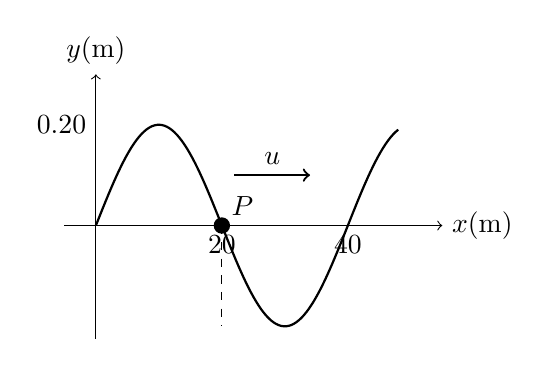
\begin{tikzpicture}[scale=0.08]
  \draw[->] (-5,0) -- (55,0) node[right] {\(x(\si{m})\)};
  \draw[->] (0,-18) -- (0,24) node[above] {\(y(\si{m})\)};
  \draw[thick,domain=0:48,samples=120] plot(\x,{16*sin(9*\x)});
  \draw[->,thick] (22,8) -- (34,8) node[midway,above] {\(u\)};
  \draw[dashed] (20,0) -- (20,-16);
  \fill (20,0) circle (1.3) node[above right] {\(P\)};
  \node[left] at (0,16) {\(0.20\)};
  \node[below] at (20,0) {\(20\)};
  \node[below] at (40,0) {\(40\)};
\end{tikzpicture}
\end{center}
\end{exercise}

\begin{solution}
\textbf{起手判断/模型：} 图像给的是 \(t=0\) 的空间波形，不是某一点的位移时间图。先从图中读出 \(\lambda\)，再由 \(u=\lambda/T\) 得到角频率；沿 \(+x\) 传播时波函数取 \(\omega t-kx+\varphi_0\) 的形式。

\textbf{波的基本量：}
\[
T=\frac{\lambda}{u}=\frac{40}{20}=\SI{2}{s},\qquad
\omega=\frac{2\pi}{T}=\pi\,\si{rad/s},\qquad
k=\frac{2\pi}{\lambda}=\frac{\pi}{20}\,\si{rad/m}.
\]

\textbf{确定初相：} 由图知 \(t=0,x=0\) 时 \(O\) 点在平衡位置，且沿 \(+x\) 方向传播时，原点此刻正向负方向运动，对应
\[
y(0,t)=0.20\cos\left(\pi t+\frac{\pi}{2}\right).
\]
于是波函数为
\[
y(x,t)=0.20\cos\left(\pi t-\frac{\pi x}{20}+\frac{\pi}{2}\right)\quad(\si{SI}).
\]

\textbf{\(P\) 点振动：} 代入 \(x_P=\SI{20}{m}\)，得
\[
y_P(t)=0.20\cos\left(\pi t-\pi+\frac{\pi}{2}\right)
=\boxed{0.20\cos\left(\pi t-\frac{\pi}{2}\right)}\quad(\si{SI}).
\]

\textbf{结论：}
\[
\boxed{y_P=0.20\cos\left(\pi t-\frac{\pi}{2}\right)},\qquad
\boxed{y=0.20\cos\left(\pi t-\frac{\pi x}{20}+\frac{\pi}{2}\right)}.
\]

\textbf{物理检查/易错点：} \(P\) 比 \(O\) 在传播方向上靠前 \(\SI{20}{m}=\lambda/2\)，所以 \(P\) 的相位应比 \(O\) 滞后 \(\pi\)。答案中 \(+\pi/2\) 变成 \(-\pi/2\)，正好体现了这一点。
\end{solution}

\begin{exercise}[2010模拟题：由两时刻波形写原点振动方程和波函数]
图示为一平面余弦波在 \(t=0\) 与 \(t=\SI{2}{s}\) 时刻的波形。由图读出 \(\lambda=\SI{160}{m}\)，两时刻波形相对向 \(+x\) 方向平移 \(\SI{20}{m}\)，且 \(t=0\) 时原点位移为 \(A/\sqrt2\)。求：1. 坐标原点处介质质点的振动方程；2. 该波的波动表达式。

\begin{center}

\includegraphics[width=0.55\linewidth]{pdf-exercises/pdf2010-mock-q23-two-waveforms.png}
\end{center}
\end{exercise}

\begin{solution}
\textbf{起手判断/模型：} 两个时刻的波形图本质上是在告诉我们“同一相位点怎样平移”。图中 \(t=\SI{2}{s}\) 的波形比 \(t=0\) 的波形向右平移 \(\SI{20}{m}\)，所以波沿 \(+x\) 方向传播。

\textbf{波速、波数和角频率：}
\[
u=\frac{\Delta x}{\Delta t}=\frac{20}{2}=\SI{10}{m/s},\qquad
k=\frac{2\pi}{\lambda}=\frac{\pi}{80}\,\si{rad/m},
\]
\[
\omega=ku=\frac{\pi}{80}\times 10=\frac{\pi}{8}\,\si{rad/s}.
\]

\textbf{确定原点初相：} 取
\[
y_O(t)=A\cos(\omega t+\varphi_0).
\]
由图知 \(t=0\) 时
\[
y_O(0)=\frac{A}{\sqrt2}\quad\Longrightarrow\quad \cos\varphi_0=\frac{1}{\sqrt2}.
\]
又由 \(t=\SI{2}{s}\) 时原点回到平衡位置，且位移从正值向零变化，可取
\[
\varphi_0=\frac{\pi}{4}.
\]
于是
\[
\boxed{y_O(t)=A\cos\left(\frac{\pi}{8}t+\frac{\pi}{4}\right)}.
\]

\textbf{写波函数：} 波沿 \(+x\) 方向传播，故
\[
y(x,t)=A\cos(\omega t-kx+\varphi_0).
\]
代入 \(k,\omega,\varphi_0\)，得
\[
\boxed{y(x,t)=A\cos\left(\frac{\pi}{8}t-\frac{\pi}{80}x+\frac{\pi}{4}\right)}\quad(\si{SI}).
\]

\textbf{物理检查/易错点：} 代入 \(x=0\) 应退回原点振动方程；代入 \(t=0\) 时，波形的第一个波峰在 \(x=\SI{20}{m}\)，与题图相符。若只记正负号而不看两时刻平移方向，很容易把 \(-kx\) 写成 \(+kx\)。
\end{solution}

\section{由参考点用相位差法写波动方程}

这一节要解决的问题是：如果题目不给原点处的振动，而是给某个中途参考点的振动方程，该怎么办？

若已知某参考点 \(x=x_0\) 处的振动方程
\[
\begin{aligned}
y(x_0,t)&=A\cos(\omega t+\varphi_B),\\
\Delta\varphi&=k(x-x_0),\\
y(x,t)&=A\cos\left[\omega t-k(x-x_0)+\varphi_B\right].
\end{aligned}
\]

这个方法的标准步骤可以固定成三步：
\begin{enumerate}
  \item 先判断波沿正方向还是负方向传播；
  \item 再比较待求点与参考点谁在前、谁在后，判断谁相位滞后、谁相位超前；
  \item 最后用 \(k(x-x_0)\) 或等价的 \(\dfrac{2\pi}{\lambda}(x-x_0)\) 补进相位。
\end{enumerate}

\begin{note}
口头判断时，可以这样记：若波沿正方向传播，前方的点通常相位滞后，后方的点通常相位超前。先把“谁先经历同一状态”想清楚，正负号就不会只剩硬背。
\end{note}

\section{相位差与波程差}

这一节要解决的问题是：为什么波动题总爱把“相位差”和“波程差”放在一起讲，它们到底怎么换算？

波动问题中，某一点在某时刻的相位与“同相/反相”判据可压成
\[
\begin{aligned}
\varphi&=\omega t-kx+\varphi_0=\omega t-\frac{2\pi}{\lambda}x+\varphi_0,\\
\delta&=x_2-x_1,\qquad
\Delta\varphi=\frac{2\pi}{\lambda}\delta,\\
\delta&=m\lambda
\iff \Delta\varphi=2m\pi
\iff \text{两点同相},\\
\delta&=\left(m+\frac12\right)\lambda
\iff \Delta\varphi=(2m+1)\pi
\iff \text{两点反相}.
\end{aligned}
\]
若只关心“同相还是反相”，也常取它们的绝对值来比较。在同一均匀介质中，波程差就是几何路程差，所以可以直接把两点间的空间距离差换成相位差。

\begin{remark}
把波长 \(\lambda\) 看成“空间里的一个完整周期”，这部分就不难了：整波长差对应整周期差，所以同相；半波长差对应半周期差，所以反相。
\end{remark}

\section{一维波动微分方程与三维简谐波动力学方程}

这一节要解决的问题是：除了写出一个具体的波函数，我们能不能写出一条直接约束”整个波场怎样传播”的方程？

\bridge{最自然的起点不是再去盯某个质点单独怎样受力，而是先抓住“行波只是把原有图样整体搬运”的事实。若波形只是在以速度 \(u\) 平移，那么时间上快一点、空间上挪一点，本质上是在追同一个图样；正因为如此，时间变化和空间变化才会被同一速度锁在一起，最后必然同时冒出 \(\partial^2/\partial t^2\) 与 \(\partial^2/\partial x^2\) 这两类量。}

\begin{definition}[偏导数]\label{def:partial-derivative}
当一个函数同时依赖多个变量（如 \(y(x,t)\) 同时依赖位置 \(x\) 和时间 \(t\)）时，\textbf{偏导数}就是”固定其他变量不动，只对其中一个变量求导”。记号 \(\dfrac{\partial y}{\partial t}\) 表示把 \(x\) 当常数、只对 \(t\) 求导；\(\dfrac{\partial y}{\partial x}\) 表示把 \(t\) 当常数、只对 \(x\) 求导。计算规则和普通导数完全一样——只是把”不动的那些变量”视为常数即可。例如 \(y=3x^2t\)，则 \(\dfrac{\partial y}{\partial t}=3x^2\)，\(\dfrac{\partial y}{\partial x}=6xt\)。
\end{definition}

\begin{remark}
偏导数的物理含义：\(\dfrac{\partial y}{\partial t}\) 是”盯住空间某一点，看它随时间怎样变”；\(\dfrac{\partial y}{\partial x}\) 是”在某一时刻冻结画面，看波形沿空间怎样弯”。二阶偏导 \(\dfrac{\partial^2 y}{\partial t^2}\) 就是加速度，\(\dfrac{\partial^2 y}{\partial x^2}\) 就是曲率（弯曲程度）。
\end{remark}

先提醒一点：这里不是在重新研究某个质点”自己怎么振”，而是在从已知波函数里读出它必须满足的传播约束。

对一维简谐波
\[
y=A\cos\omega\left(t-\frac{x}{u}\right),
\]
分别对 \(t\) 和 \(x\) 求两次偏导，可得
\begin{note}
这里用偏导，是因为波场同时依赖空间和时间。对 \(t\) 求偏导时，把 \(x\) 固定住，表示“盯住某一点看它随时间怎样振”；对 \(x\) 求偏导时，把 \(t\) 固定住，表示“在某一时刻看波形沿空间怎样弯”。推广到三维后，\(\nabla^2\) 就是在把三个方向的空间弯曲程度加总起来。
\end{note}
\begin{align*}
\frac{\partial^2 y}{\partial t^2}
&=-\omega^2 A\cos\omega\left(t-\frac{x}{u}\right),\\
\frac{\partial^2 y}{\partial x^2}
&=-\frac{\omega^2}{u^2}A\cos\omega\left(t-\frac{x}{u}\right)
=\frac{1}{u^2}\frac{\partial^2 y}{\partial t^2}.
\end{align*}

把它读成“空间中的弯曲程度”和“时间上的变化快慢”彼此绑定，就不难了：波不是某个点单独在动，而是整列波形在传播，所以空间曲率和时间加速度必须同步出现。

这条方程说明：波形在空间中的弯曲程度，与它在时间上的加速变化直接相关。它约束的不是某一个点怎样振，而是\textbf{整列波在时空中怎样传播}，所以它常被称为波动的动力学方程。

若把一维推广到三维，设介质扰动量为 \(\xi=\xi(x,y,z,t)\)，则
\begin{align*}
\nabla^2\xi&=\frac{1}{u^2}\frac{\partial^2 \xi}{\partial t^2},\\
\nabla^2&=\frac{\partial^2}{\partial x^2}
+\frac{\partial^2}{\partial y^2}
+\frac{\partial^2}{\partial z^2},
\end{align*}
其中 \(\nabla^2\) 叫做拉普拉斯算符。

\bridge{如果你还没学过多元微积分中的梯度和散度：\(\nabla^2\) 可以先理解为"对三个方向各求一次二阶偏导再加起来"，它衡量的是函数值在某点相对于周围邻域平均值的偏离程度。一维时 \(\nabla^2=\partial^2/\partial x^2\) 就是曲线的"弯曲程度"；三维时把三个方向的弯曲加总。}

\begin{note}
这里的 \(y(x,t)\) 是一维情形下的位移函数，而 \(\xi(x,y,z,t)\) 是三维波场里的一个标量扰动量。对不同物理问题，\(\xi\) 具体可以代表位移、压强扰动等，但它们都满足同一类波动方程。
\end{note}

\section{球面简谐波}

点波源向各个方向均匀发出波时，形成球面波。若介质没有吸收，波通过任意球面的平均能流相同，而球面面积随 \(r^2\) 增大，因此振幅会随距离减小：
\[
\begin{aligned}
A(r)&\propto \frac{1}{r},\qquad
A(r)=A_0\frac{r_0}{r},\\
y(r,t)&=A_0\frac{r_0}{r}\cos\omega\left(t-\frac{r}{u}\right),\qquad r>r_0.
\end{aligned}
\]

\bridge{球面波振幅越传越小，并不是某个质点“自己变弱了”，而是因为同样多的能量被摊到了越来越大的球面上。}

\section{机械波的能量}

这一节要解决的问题是：机械波明明只是“振动状态在传播”，为什么还能把能量从一处送到另一处？

\textbf{先把单个振子的能量图景平移过来。} 对波里的某一个微小体积元，仍然应该先问两件事：它自己此刻振得多快？它和相邻部分之间被拉伸、压缩得多厉害？前者决定动能，后者决定弹性势能。

\textbf{第一项为什么看 \(\partial y/\partial t\)。} 若位移场写成 \(y(x,t)\)，那么盯住空间中某个固定位置 \(x\)，这个体积元的振动速度就是
\[
v=\frac{\partial y}{\partial t}.
\]
而这个体积元自己的质量就是 \(dm=\rho\,\dd V\)，因此它的动能自然写成
\[
\dd E_k=\frac12 \rho\left(\frac{\partial y}{\partial t}\right)^2\dd V.
\]

\textbf{第二项为什么看 \(\partial y/\partial x\)，而不是直接看 \(y\)。} 因为弹性势能并不取决于“整段介质整体挪了多远”，而取决于“相邻两点有没有被拉开或挤近”。若整根棒每一点都平移同样的位移 \(y\)，虽然 \(y\) 本身可能很大，但相邻两点间距没变，介质根本没有形变，也就没有额外弹性势能。真正记录形变程度的，是相邻位移之差除以原长度，也就是应变：
\[
\varepsilon=\frac{\Delta l}{\dd x}=\frac{\partial y}{\partial x}.
\]
再结合杨氏模量关系 \(\sigma=Y\varepsilon\)，并记住线性弹性范围内单位体积储存的弹性势能密度本来就来自
\[
\int_0^\varepsilon \sigma\,\dd\varepsilon
=\int_0^\varepsilon Y\varepsilon\,\dd\varepsilon
=\frac12 \sigma\varepsilon,
\]
于是体积元中的弹性势能自然写成
\[
\dd E_p=\frac12 \sigma\varepsilon\,\dd V
=\frac12 Y\left(\frac{\partial y}{\partial x}\right)^2\dd V.
\]
于是体积元的总机械能就是
\[
\dd E=\dd E_k+\dd E_p.
\]
也就是说，在真正读公式之前，脑中最好已经先分清：\textbf{时间导数记录局部运动，空间导数记录局部形变。} 这样看到 \(\partial y/\partial t\) 和 \(\partial y/\partial x\) 时，就不会像在看两块凭空冒出来的符号。

\textbf{把它代到简谐行波里之前，还可以先预判结果的大致结构。} 因为对简谐行波来说，无论对时间求导还是对空间求导，都会把位移振幅 \(A\) 变成与 \(A\omega\) 同量级的量；而能量本来又是二次量，所以最后的动能、势能和总能量里一定会出现 \(A^2\omega^2\)。先有这个预判，再读结果就顺了。以固体棒中传播的平面简谐纵波为例，若这是沿棒传播的平面简谐纵波
\begin{align*}
y&=A\cos\omega\left(t-\frac{x}{u}\right),\qquad u=\sqrt{\frac{Y}{\rho}},\\
\frac{\partial y}{\partial t}&=-A\omega\sin\omega\left(t-\frac{x}{u}\right),&
\frac{\partial y}{\partial x}&=\frac{A\omega}{u}\sin\omega\left(t-\frac{x}{u}\right),\\
\dd E_k&=\frac12 \rho A^2\omega^2\sin^2\omega\left(t-\frac{x}{u}\right)\dd V,&
\dd E_p&=\frac12 \rho A^2\omega^2\sin^2\omega\left(t-\frac{x}{u}\right)\dd V,\\
\dd E&=\dd E_k+\dd E_p=\rho A^2\omega^2\sin^2\omega\left(t-\frac{x}{u}\right)\dd V.
\end{align*}

\textbf{最后再看局部机械能为什么不守恒。} 上式表明，同一个体积元的机械能会随时间起伏变化。它有时从前面的介质接收能量，有时又把能量交给后面的介质，所以
\begin{itemize}
  \item 任一体积元都在不断地接收和放出能量；
  \item 任一体积元的机械能不守恒；
  \item 波动是能量传递的一种方式。
\end{itemize}

\begin{note}
这正是波的能量部分最该抓住的一句话：\textbf{对整列行波来说，能量在向前传播；对局部体积元来说，它自己的机械能却不守恒。} 这和单个简谐振子的“总能量守恒”正好形成鲜明对照。
\end{note}

\begin{exercise}[2008级期末：行波中质元总能量与动能的关系]
一平面简谐机械波在媒质中传播时，若某一媒质质元在 \(t\) 时刻的总机械能为 \(\SI{10}{J}\)，求在 \(t+T\) 时刻该质元的振动动能，其中 \(T\) 为波的周期。
\end{exercise}

\begin{solution}
\textbf{起手判断/模型：} 对行波中的一个质元，动能和弹性势能会随时间同步变化。对平面简谐行波，某一瞬间同一体积元的动能与弹性势能相等，而质元的运动状态经过一个周期后完全重复。

\textbf{主方程：}
\[
E=E_k+E_p,\qquad E_k=E_p.
\]

\textbf{分步代入或化简：} 题目给 \(t\) 时刻总机械能为 \(\SI{10}{J}\)。经过一个周期后，质元位移、速度和形变状态都回到同一相位，所以总机械能仍为 \(\SI{10}{J}\)。又因为行波中该瞬时
\[
E_k=E_p=\frac{E}{2},
\]
于是
\[
E_k(t+T)=\frac{10}{2}=\SI{5}{J}.
\]

\textbf{结论：}
\[
\boxed{E_k(t+T)=\SI{5}{J}}.
\]

\textbf{物理检查/易错点：} 不要把波中质元误当成孤立弹簧振子。孤立简谐振子的总能量守恒且动能、势能交替；行波中局部质元的能量随相位起伏，但动能和弹性势能在同一瞬时相等。
\end{solution}

\section{能流和能流密度}

上一节已经得到体积元的总机械能 \(\dd E\)。接下来最自然的两个问题是：某处\textbf{平均每单位体积装了多少能量}？这些能量又\textbf{每秒穿过某截面多少}？

先回答第一个问题。这里横线 \(\bar{\phantom{w}}\) 统一表示\textbf{对一个周期做时间平均}。上一节已经知道瞬时能量密度随 \(\sin^2\) 起伏，所以一做周期平均，唯一会发生的事情就是把 \(\sin^2\) 的平均值换成 \(1/2\)。先有这句预判，再看平均能量密度公式就不会突兀。由定义立刻有能量密度
\[
\begin{aligned}
w&=\frac{\dd E}{\dd V}
=\rho A^2\omega^2\sin^2\omega\left(t-\frac{x}{u}\right),\\
\bar w&=\frac12 \rho\omega^2A^2.
\end{aligned}
\]
\bridge{这个公式不必死背成一串字母。它说的其实很朴素：介质越重、振得越快、摆得越大，单位体积里储存和交换的波动能量就越多。}

\begin{note}
\textbf{先看什么信号：} 题目若在比较“波送能快不快”“单位面积每秒通过多少能量”，就该从 \(\bar P\) 或 \(I\) 入手，而不是盯某个质点瞬时速度；\textbf{这条公式在控制什么：} \(\bar w\) 管单位体积平均存了多少波动能量，\(\bar P\) 管整列波每秒送过多少能量，\(I\) 管单位面积上的输运强弱；\textbf{怎样最快记住：} 先看一小块介质里装了多少，再想“平面波每秒会扫过厚度 \(u\Delta t\) 的一薄层”，于是乘波速 \(u\) 就变成“每秒送走多少”，最后除面积得到 \(I=\bar wu\)；\textbf{最容易错：} 把 \(u\) 当成质点振动速度，或把“振幅变 2 倍”误判成“能流密度也只变 2 倍”。
\end{note}

再回答第二个问题。仅仅知道“某处存了多少能量”还不够，我们还想知道“能量穿过某个截面的速度有多快”。于是引入\textbf{能流} \(P\)：单位时间内垂直通过某一面积的能量。这里最该先在脑中立起来的图景是：既然单位体积平均装了 \(\bar w\)，那么每秒真正能穿过截面的，不过就是“厚度为 \(u\Delta t\) 的那一层波”。所以能流必然等于“每单位体积的平均能量”乘“每秒扫过的体积”，能流密度再把面积除掉就行。带着这个图景，再看下面的式子：
\[
\begin{aligned}
\Delta E&=\bar w Su\Delta t
\implies
\bar P=\frac{\Delta E}{\Delta t}
=\bar w uS=\frac12 \rho\omega^2A^2uS,\\
I&=\frac{\bar P}{S}=\bar w u=\frac12 \rho\omega^2A^2u
\implies
I\propto \rho,\qquad
I\propto \omega^2,\qquad
I\propto A^2,\qquad
I\propto u.
\end{aligned}
\]

\begin{remark}
这里的 \(u\) 是波速，不是某个质点自己的振动速度。能流密度在乎的是“每秒有多厚的一层已带能量的介质扫过截面”，所以它跟波形传播速度有关，而不是跟单个质点一上一下振得多快直接等同。
\end{remark}

\begin{exercise}[振幅加倍时能流密度怎样变]
若同一介质中两列简谐波的波速和频率都相同，但第二列波的振幅是第一列的 2 倍，求两列波平均能流密度之比。
\end{exercise}

\begin{solution}
\textbf{起手判断/模型：} 这道题不是要求绝对数值，而是在同一介质、同一频率下比较两列波的能流密度之比，所以最稳的做法是先找出\textbf{哪些量相同、哪些量在变}，再用比例关系。

\textbf{主方程与化简：} 题目已说明两列波在同一介质中传播，且波速和频率相同，因此
\[
I=\frac{1}{2}\rho\omega^2A^2u,\qquad
\rho,\ \omega,\ u \text{ 都相同 } \implies I\propto A^2
\implies
\frac{I_2}{I_1}=\frac{A_2^2}{A_1^2}
=\frac{(2A_1)^2}{A_1^2}=4.
\]

\textbf{结论：} 第二列波的平均能流密度是第一列的 \(4\) 倍。

\textbf{物理检查/易错点：} 这里比较的是能流密度，不是质点瞬时速度；同一介质、同一频率时，真正起作用的是振幅平方。最常见误判是把“振幅变成 \(2\) 倍”直接写成“能流密度也变成 \(2\) 倍”。
\end{solution}

\section{惠更斯原理}

\textbf{本节问题：} 当我们只知道“已有一个波前”，为什么还能继续预言下一时刻的新波前会在哪里？

\textbf{物理图景：} 若把整个波前当成一块刚性板，就很难解释波为何会绕过障碍物、在边缘重新铺开。更自然的想法是：波前上每一点都像一个微小的新波源，都会继续把振动向外传。于是下一时刻真正决定新波前位置的，就不再是旧波前整体的“平移”，而是这些子波共同包出的新外沿。

\begin{theorem}[惠更斯原理]
波阵面上的每一点都可以看成发出子波的新波源；经过一段时间后，这些子波的包络面就是新的波前。
\end{theorem}

这一原理的意义有两层：一层是帮助我们直观理解“为什么波会继续向前传播”；另一层是帮助我们解释反射、折射和衍射等现象中的新波前如何形成。

\begin{note}
看到“包络面”不要害怕，它只是说：把每个子波都画出来后，外面那层刚好与它们相切的轮廓，就是下一时刻的新波前。
\end{note}

\section{波的衍射}

\textbf{本节问题：} 波为什么不会像小球那样被障碍物整齐截断，而会拐进“本来该是阴影”的区域？

\textbf{物理图景：} 当波前来到孔缝或障碍物边缘时，真正被继续推进的不是一条刚性的几何边界，而是边缘附近那一段还活着的波前。按惠更斯观点，这段波前上的各点仍会发出子波，因此阴影区里并不是“完全没有后续波源”，而是会收到这些边缘子波的叠加。

\textbf{核心判据/公式：} 先不用急着背具体条纹条件，最先要记的是一条定性判据：\textbf{波长与障碍物特征尺寸可比时，衍射才会明显。} 常用经验判断可压成
\[
\lambda\sim a \text{ 或 } \lambda>a \implies \text{衍射显著},\qquad
\lambda\ll a \implies \text{几何直进近似更好},
\]
其中 \(a\) 可以代表孔径、缝宽或障碍物尺度。

\textbf{公式为何这样写：} 若 \(\lambda\) 相对 \(a\) 很小，边缘附近能“抹开”到阴影区的角范围就很窄，于是看起来几乎还是直线前进；若 \(\lambda\) 与 \(a\) 同量级，边缘子波的贡献就不再只是小修正，而会主导后方图样。

\textbf{常见误判或适用边界：} “看见明显拐弯”才叫衍射，这种理解太窄。只要孔缝限制了波前、图样不再能用纯几何直进解释，就已经进入衍射问题。后面光学里的单缝、圆孔和分辨率，本质上都在重复这里的判断线。

\section{波的反射和折射}

这一节最该先放进脑中的，不是角度公式本身，而是\textbf{为什么方向会改。} 当波前的一部分先碰到边界、先进入另一种介质时，这一部分若传播得更快或更慢，整条波前就会被“转一下方向”；这个几何后果翻译到光线语言里，才表现成反射角、折射角这些关系。所以反射、折射角公式本质上都在记“波前不同部分推进快慢不一样”这一件事。

当机械波遇到两种介质的分界面时，会发生反射；若一部分波进入另一种介质，还会发生折射。

\bridge{把一条波前想成一排同步前进的小点最容易理解。若只是反射，这些点仍回到原介质里传播，速度大小没变，只是法向分量翻了方向，于是图样关于法线镜面对称，这就是反射角等于入射角。若有一部分进入另一介质，先进入的一边改用新速度前进，整条波前就会转向，于是才有折射角关系。}

这里的入射角、反射角和折射角都统一约定为\textbf{相对界面法线}来量，而不是相对界面本身来量。

反射与折射的基本规律可并排记成
\[
\begin{aligned}
\text{反射：}\quad &\text{入射线、反射线和界面法线共面},\qquad \text{反射角}=\text{入射角},\\
\text{折射：}\quad &\text{入射线、折射线和界面法线共面},\qquad \frac{\sin i}{\sin r}=\frac{u_1}{u_2}.
\end{aligned}
\]

这条折射关系很值得直观理解：如果第二种介质中波速更小，即 \(u_2<u_1\)，那么折射线会向法线偏折；若 \(u_2>u_1\)，则会偏离法线。

\begin{note}
这里是波的一般规律，后面光学里讲反射和折射时，只是把机械波换成了光波，把波速差换成了折射率差。
\end{note}

\section{波的叠加原理}

\textbf{本节问题：} 两列波在同一位置相遇时，究竟是“打架后改头换面”，还是只是暂时把位移加在一起？

\textbf{物理图景：} 对线性介质来说，一列波单独能造成怎样的位移，另一列波也照样能单独造成自己的位移；两者同时到来时，介质只是在那一瞬间同时响应这两份作用，于是位移应当直接相加。关键是这种相加只发生在“此时此地”的响应上，并不意味着两列波会永久融合成一列新波。

\begin{definition}[波的叠加原理]
在几列波相遇的区域内，任一点的振动位移，等于各列波单独存在时在该点所引起位移的矢量和。
\end{definition}

\bridge{这一定律最该这样读：相遇时先\textbf{加位移}，相遇后再\textbf{各走各的}。对线性波动，叠加只是同一时刻同一点上的暂时合成，不是把两列波永久揉成一列新波。}

这一定律包含两层重要意思：
\begin{itemize}
  \item 相遇时，位移可以直接相加；
  \item 相遇之后，各列波仍保持原来的频率、波长、振幅和传播方向继续前进，好像没有彼此永久“缠住”一样。
\end{itemize}

\begin{remark}
很多人会误以为“两列波撞上以后会混成一列新波”。对线性波动而言，真正发生的是\textbf{暂时叠加}，不是永久改写。
\end{remark}

\section{波的双缝干涉}

这一节要解决的问题是：为什么两列相干波相遇后，会在有些地方总是加强、在有些地方总是减弱？

这类题真正的第一动作不是先盯“亮还是暗”，而是先问：观察点 \(P\) 处，这两列波到达时到底相差了多少路程、于是又相差了多少相位？只要这一步定下来，后面的“相长还是相消”就只是相位判据的直接翻译。因此双缝干涉的主线可以一直压成一句话：\textbf{先算波程差，再换相位差，最后判加强还是减弱。}

若两条狭缝 \(S_1,S_2\) 发出两列\textbf{频率相同且相位差恒定}的相干波，则在空间某点 \(P\) 处可写成
\[
\begin{aligned}
y_1&=A\cos(\omega t-kr_1),\qquad
y_2=A\cos(\omega t-kr_2),\\
\delta&=r_2-r_1,\qquad
\Delta\varphi=\frac{2\pi}{\lambda}\delta,\\
\delta&=m\lambda
\implies \Delta\varphi=2m\pi \qquad \text{两列波相长},\\
\delta&=\left(m+\frac12\right)\lambda
\implies \Delta\varphi=(2m+1)\pi \qquad \text{两列波相消}.
\end{aligned}
\]

\begin{note}
这就是后面光学双缝干涉的母版。第 6 章先抓住本质：\textbf{先找两列相干波，再算波程差，再判相长还是相消。} 这样后面换成光波时，只是在同一框架里换对象。
\end{note}

\begin{exercise}[两相干波源在点 \(P\) 处为什么会完全相消]
同一介质中有两相干波源 \(A,B\)，振幅都为 \(\SI{5}{cm}\)，频率都为 \(\SI{100}{Hz}\)，波速为 \(\SI{10}{m/s}\)。已知 \(AP=\SI{15}{m}\)、\(BP=\SI{25}{m}\)，且当 \(A\) 为波峰时 \(B\) 恰为波谷。求点 \(P\) 的干涉结果。
\end{exercise}

\begin{solution}
\textbf{起手判断/模型：} 题目一边给了“同相还是反相”的初始信息，一边给了两条传播路程，所以第一条方程应先落在“初相差 + 传播相位差”的总账上，而不是先猜结果。

\textbf{主方程：}
\[
\lambda=\frac{u}{\nu},\qquad
\Delta\varphi_P=\Delta\varphi_0-\frac{2\pi}{\lambda}(AP-BP).
\]

\textbf{分步代入或化简：} 由题意，
\[
\lambda=\frac{10}{100}=\SI{0.10}{m},\qquad \Delta\varphi_0=\pi.
\]
又因为
\[
AP-BP=15-25=-\SI{10}{m}=-100\lambda,
\]
所以
\[
\Delta\varphi_P
=\pi-\frac{2\pi}{\lambda}(-10)
=\pi+200\pi
=201\pi.
\]
这仍然是奇数个 \(\pi\)，因此两列波在 \(P\) 点始终反相；又因为两源振幅相等，故
\[
A_P=\abs{A_1-A_2}=0.
\]

\textbf{结论：} 点 \(P\) 处始终相消，合振幅为 \(0\)，因此 \(P\) 点保持静止。

\textbf{物理检查/易错点：} 这题最容易错在把“路程差很大”误以为“结果很复杂”。其实只要路程差恰好是整数个波长，它对“相长还是相消”只留下模 \(2\pi\) 的效果；真正决定本题的是“初相反”这一条。
\end{solution}

\begin{exercise}[两相干波源连线上哪些位置始终加强]
两相干波源 \(s_1,s_2\) 相距 \(l=\SI{10}{m}\)，振幅都为 \(\SI{0.02}{m}\)，频率为 \(\SI{5}{Hz}\)，波速为 \(\SI{10}{m/s}\)，初相相同。求两源连线上振动加强的位置及其合振幅，并判断右侧延长线上合振动怎样。
\end{exercise}

\begin{solution}
\textbf{起手判断/模型：} 两源初相相同，所以这题第一步先写波长，再把“振动加强”直接翻成“波程差为整数个波长”。

\textbf{主方程：}
\[
\lambda=\frac{u}{\nu},\qquad
\abs{r_1-r_2}=k\lambda.
\]

\textbf{分步代入或化简：} 先算波长：
\[
\lambda=\frac{10}{5}=\SI{2}{m}.
\]
设连线上一点距 \(s_1\) 为 \(x\)，则
\[
r_1=x,\qquad r_2=l-x=10-x.
\]
振动加强条件给出
\[
\abs{x-(10-x)}=2k
\implies \abs{2x-10}=2k
\implies x=5\pm k.
\]
再结合 \(0\le x\le 10\)，得
\[
k=0,1,2,3,4,5
\implies x=0,1,2,3,4,5,6,7,8,9,10\ \si{m}.
\]
由于两列波振幅相等且同相加强，故这些位置的合振幅都为
\[
A=2A_1=\SI{0.04}{m}.
\]
对右侧延长线上的任一点，波程差恒为
\[
r_1-r_2=l=\SI{10}{m}=5\lambda,
\]
所以始终满足加强条件。

\textbf{结论：} 两源连线上从 \(x=0\) 到 \(x=\SI{10}{m}\) 的整数米位置都振动加强，合振幅为 \(\SI{0.04}{m}\)；右侧延长线上也始终加强。

\textbf{物理检查/易错点：} 延长线题最容易错在把波程差写成“随点变化”。其实在右侧延长线上，两源到该点的路程之差始终就是源间距 \(l\)，先认出这件事，题就会非常短。
\end{solution}

\begin{exercise}[两相干波源有初相差时为什么左右延长线不一样]
两相干波源 \(s_1,s_2\) 振幅相同，且 \(s_2\) 比 \(s_1\) 的初相超前 \(\pi/2\)。已知两源间距 \(l=\lambda/4\)。讨论两源连线左侧延长线与右侧延长线上的干涉情况。
\end{exercise}

\begin{solution}
\textbf{起手判断/模型：} 这题和“同相两源”的关键区别，不在几何上，而在一开始就自带初相差 \(\pi/2\)。所以第一步应先把\textbf{初相差}和\textbf{波程差导致的相位差}记到同一本总账里：
\[
\Delta\varphi=(\varphi_2-\varphi_1)-\frac{2\pi}{\lambda}(r_2-r_1).
\]
左右延长线之所以结论不同，就是因为 \(r_2-r_1\) 的符号会反过来。

\textbf{主方程：}
\[
\varphi_2-\varphi_1=\frac{\pi}{2},\qquad
\Delta\varphi=(\varphi_2-\varphi_1)-\frac{2\pi}{\lambda}(r_2-r_1).
\]

\textbf{分步代入或化简：} 在左侧延长线上，点 \(P\) 到右侧波源更远，因此
\[
r_2-r_1=l=\frac{\lambda}{4}.
\]
于是
\[
\Delta\varphi=\frac{\pi}{2}-\frac{2\pi}{\lambda}\cdot\frac{\lambda}{4}=0,
\]
对应相长干涉，合振幅为
\[
A=2A_1.
\]
在右侧延长线上，路程差符号反过来：
\[
r_2-r_1=-l=-\frac{\lambda}{4},
\]
因此
\[
\Delta\varphi=\frac{\pi}{2}-\frac{2\pi}{\lambda}\cdot\left(-\frac{\lambda}{4}\right)=\pi,
\]
对应相消干涉，合振幅为
\[
A=0.
\]

\textbf{结论：} 左侧延长线上始终加强，右侧延长线上始终减弱到完全相消。

\textbf{物理检查/易错点：} 这题最值得记住的不是结论本身，而是“延长线两边不对称”的原因：\textbf{初相差固定，但几何路程差在左右两边符号相反。} 只要先把这个符号问题写清，题就不会乱。
\end{solution}

\section{驻波的产生}

这一节要解决的问题是：为什么两列明明都在传播的行波，叠加后会出现一种“看起来站住了”的波？

两列\textbf{同频、同振幅、沿相反方向传播的相干波}叠加，可以形成驻波。驻波之所以特殊，不是因为质点不动，而是因为波峰波谷的整体图样不再向前平移。

从形成条件看，驻波本质上是一种特殊的干涉现象；从实际产生方式看，最常见的来源就是\textbf{入射波在边界上反射后，与反射波叠加}。

\begin{remark}
纯自学时最容易误会成“驻波就是不会动的波”。其实驻波里的每个非波节点都在动，只是整个图样不再向前跑，所以你看不到行波那种波峰波谷一路前进的效果。
\end{remark}

\section{驻波方程}

既然驻波来自两列等振幅、反向传播的行波，那么最自然的想法就是：先把两列行波并排写出，再问相加后能不能把“只跟位置有关的部分”和“只跟时间有关的部分”拆开。和差化积之所以在这里突然变得关键，正是因为它能把两个反向传播的相位组合，压成一个空间振幅因子乘一个时间振动因子。这样一来，“哪些地方永远振幅大、哪些地方永远振幅零”就会自动从公式里露出来。

设两列等振幅行波分别为
\[
\begin{aligned}
y_1&=A\cos(\omega t-kx),\qquad
y_2=A\cos(\omega t+kx),\\
y&=y_1+y_2=2A\cos kx\cos\omega t.
\end{aligned}
\]
这就是一个典型的驻波方程。

它有两个非常重要的特征：振幅不再是常量，而是随位置变化；各质点仍然都作同频简谐振动，但不同位置的振幅不同。由上式可压成
\[
\begin{aligned}
A_{\text{驻}}(x)&=2A\abs{\cos kx},\\
kx=n\pi
&\Longrightarrow
x=n\frac{\lambda}{2}\qquad \text{(波腹)},\\
kx=\left(n+\frac12\right)\pi
&\Longrightarrow
x=\left(n+\frac12\right)\frac{\lambda}{2}
=\frac{(2n+1)\lambda}{4}\qquad \text{(波节)}.
\end{aligned}
\]

因此，相邻两波腹间距和相邻两波节间距都等于 \(\lambda/2\)，相邻波节与波腹间距等于 \(\lambda/4\)。

在相位关系上，驻波也很特殊：相邻两波节之间的所有质点同相振动，而跨过一个波节后，两侧振动会相反，相当于在波节处出现 \(\pi\) 的相位突变。

\begin{note}
驻波虽然由两列行波叠加而成，但它\textbf{没有净能量向某一个方向持续传播}。行波传的是“振动状态和能量一起前进”，驻波只留下了“空间中的固定振动图样”。
\end{note}

\begin{exercise}[2010级期末：由驻波方程判断两点振动相位差]
一驻波表达式为
\[
y=A\cos 2\pi x\cos 100\pi t\quad(\mathrm{SI}).
\]
求位于 \(x_1=\frac18\,\si{m}\) 的质元 \(P_1\) 与位于 \(x_2=\frac38\,\si{m}\) 的质元 \(P_2\) 的振动相位差。
\end{exercise}

\begin{solution}
\textbf{起手判断/模型：} 驻波中每个固定位置的质元都作简谐振动，但空间因子 \(\cos 2\pi x\) 的正负会决定该点与公共时间因子是同相还是反相。

\textbf{代入空间因子：}
\[
\cos(2\pi x_1)=\cos\frac{\pi}{4}>0,
\]
\[
\cos(2\pi x_2)=\cos\frac{3\pi}{4}<0.
\]
两点的空间因子一正一负，因此它们的时间振动相差一个负号。

\textbf{结论：}
\[
\boxed{\Delta\varphi=\pi}.
\]

\textbf{物理检查/易错点：} 驻波题不要把两点间距直接当成行波的波程差。更稳的是看驻波空间因子的符号；符号相反就表示两点反相。
\end{solution}

\section{反射点为波节还是波腹}

这一节要解决的问题是：边界反射以后，原点到底该当成波节还是波腹？

关键不在“有没有反射”，而在\textbf{反射后是否反相}。

若把入射波写成
\[
\begin{aligned}
y_i&=A\cos(\omega t-kx),\\
\text{波节边界:}\quad
y_r&=A\cos(\omega t+kx-\pi)
\implies y=2A\sin kx\,\sin\omega t,\\
\text{波腹边界:}\quad
y_r&=A\cos(\omega t+kx)
\implies y=2A\cos kx\,\cos\omega t.
\end{aligned}
\]
于是 \(x=0\) 处始终有 \(y=0\) 时边界是波节，\(x=0\) 处振幅最大时边界是波腹。

\begin{note}
固定端反射通常对应波节，自由端反射通常对应波腹。很多题做错，不是驻波公式不会，而是一开始就把“边界是节点还是腹点”判反了。
\end{note}

\section{相位突变与半波损失}

这一节要解决的问题是：为什么有些反射会突然多出一个 \(\pi\) 的相位反转？

当波从\textbf{波疏介质}垂直入射到\textbf{波密介质}，再反射回波疏介质时，反射点形成波节。此时入射波与反射波在边界处总是反相，所以反射波相当于多了一个
\(\pi \iff \frac{\lambda}{2}\)。
也就是说，相位突变 \(\pi\) 等效于附加了 \(\lambda/2\) 的波程差，这就叫\textbf{半波损失}。

反过来，当波从\textbf{波密介质}垂直入射到\textbf{波疏介质}并被反射回去时，反射点形成波腹，入射波和反射波在边界处同相，因此\textbf{不发生相位突变}，也就没有半波损失。

\begin{remark}
这部分特别值得提前记牢，因为后面光学里的薄膜干涉也会反复出现“半波损失”这个思想。机械波和光波的对象不同，但“相位是否翻转、是否等效多了半个波长”这条判断线是同一条。
\end{remark}

\begin{exercise}[反射后再与另一列波相遇时怎样先记半波损失]
两列相干波 \(A,B\) 的波长都为 \(\lambda\)。波 \(A\) 经过 \(O_1\) 后在点 \(m\) 处反射，再传播到点 \(P\)；波 \(B\) 从 \(O_2\) 直接传播到 \(P\)。已知 \(O_1m+mp=8\lambda\)、\(O_2P=3\lambda\)，反射处有半波损失，两源在 \(O_1,O_2\) 处的振动都为 \(y=A\cos \pi t\)。求两列波在 \(P\) 点的振动方程以及 \(P\) 点合振动。
\end{exercise}

\begin{solution}
\textbf{起手判断/模型：} 题目关键不在路程长短本身，而在波 \(A\) 多经过了一次反射，所以总相位里必须先把半波损失补进去。最稳的写法是把每一路到 \(P\) 的总相位直接写出来。

\textbf{主方程：}
\[
y_P=A\cos\!\left(\pi t-\frac{2\pi}{\lambda}r+\varphi_{\text{反}}\right),
\qquad
\varphi_{\text{反}}=
\begin{cases}
\pi,&\text{有半波损失},\\
0,&\text{无半波损失}.
\end{cases}
\]

\textbf{分步代入或化简：} 对波 \(A\)，总传播路程为 \(8\lambda\)，且反射时多出一项 \(\pi\)，因此
\[
y_A(P,t)=A\cos\!\left(\pi t-\frac{2\pi}{\lambda}\cdot 8\lambda-\pi\right)
=A\cos(\pi t-17\pi)
=-A\cos\pi t.
\]
对波 \(B\)，总传播路程为 \(3\lambda\)，无额外相位突变，所以
\[
y_B(P,t)=A\cos\!\left(\pi t-\frac{2\pi}{\lambda}\cdot 3\lambda\right)
=A\cos(\pi t-6\pi)
=A\cos\pi t.
\]
于是
\[
y_P=y_A+y_B=-A\cos\pi t+A\cos\pi t=0.
\]

\textbf{结论：} 两列波在 \(P\) 点的振动分别为 \(y_A=-A\cos\pi t\)、\(y_B=A\cos\pi t\)，故 \(P\) 点合振动恒为 \(0\)。

\textbf{物理检查/易错点：} 若漏掉半波损失，本题会被误判为同相加强。反射题最重要的不是把每一段路机械相加，而是先问“这次反射到底翻没翻相”。
\end{solution}

\begin{exercise}[已知一列行波时怎样补出形成驻波的反向波]
弦线上有一简谐波
\[
y_1=2.0\times10^{-2}\cos\!\left[2\pi\left(\frac{t}{0.02}-\frac{x}{20}\right)+\frac{\pi}{3}\right]\ (\si{SI}).
\]
若要在这条弦上形成驻波，并要求 \(x=0\) 处为波节，求还应叠加哪一列简谐波。
\end{exercise}

\begin{solution}
\textbf{起手判断/模型：} 要形成驻波，补上的那列波必须与已知波\textbf{同频、同振幅、反向传播}。而“\(x=0\) 处为波节”不是后置检查，而是用来定反向波初相的关键条件。

\textbf{主方程：} 设所求反向波为
\[
y_2=2.0\times10^{-2}\cos\!\left[2\pi\left(\frac{t}{0.02}+\frac{x}{20}\right)+\varphi\right].
\]

\textbf{分步代入或化简：} 将两列波相加，用和差化积整理：
\[
\begin{aligned}
y&=y_1+y_2\\
&=4.0\times10^{-2}
\cos\!\left[\frac12\left(\frac{2\pi x}{20}+\varphi-\frac{\pi}{3}\right)\right]
\cos\!\left[\frac12\left(\frac{4\pi t}{0.02}+\varphi+\frac{\pi}{3}\right)\right].
\end{aligned}
\]
要使 \(x=0\) 处为波节，就必须让驻波振幅因子在 \(x=0\) 为零，即
\[
\cos\!\left[\frac12\left(\varphi-\frac{\pi}{3}\right)\right]=0
\implies
\frac12\left(\varphi-\frac{\pi}{3}\right)=\frac{\pi}{2}
\implies
\varphi=\frac{4\pi}{3}.
\]

\textbf{结论：} 所求简谐波为
\[
y_2=2.0\times10^{-2}\cos\!\left[2\pi\left(\frac{t}{0.02}+\frac{x}{20}\right)+\frac{4\pi}{3}\right].
\]

\textbf{物理检查/易错点：} 本题最容易错在只顾“反向传播”，却忘了驻波还要满足指定边界条件。驻波题里，方向负责搭架子，边界条件负责定相位。
\end{solution}

\begin{exercise}[波阻更大时反射波为什么要先带一个 \(\pi\)]
一列沿 \(x\) 轴正向传播的简谐波为
\[
y_1=10^{-3}\cos\!\left[200\pi\left(t-\frac{x}{200}\right)\right]\ (\si{m}).
\]
设介质 \(1\) 与介质 \(2\) 的分界点为 \(A\)，且 \(OA=L=\SI{2.25}{m}\)。已知介质 \(2\) 的波阻大于介质 \(1\)，反射波与入射波振幅相等。求：1. 反射波方程；2. 驻波方程；3. \(OA\) 之间波节与波腹的位置坐标。
\end{exercise}

\begin{solution}
\textbf{起手判断/模型：} “波阻更大”这四个字不是背景信息，而是在告诉你：反射端等效为\textbf{波节边界}，所以反射波在边界处相对入射波要多出一个 \(\pi\) 的相位突变。也就是说，这题第一步不是直接猜常数，而是先把“固定端式反相反射”认出来。

\textbf{主方程：} 设反射波为
\[
y_2=10^{-3}\cos\!\left[200\pi\left(t+\frac{x}{200}\right)+\varphi_0\right].
\]
在 \(x=L\) 的边界点 \(A\) 上，反射波应与入射波反相，因此
\[
y_2(A,t)=y_1(A,t+\text{同一时刻})\text{ 的反号}
=10^{-3}\cos\!\left[200\pi\left(t-\frac{L}{200}\right)+\pi\right].
\]

\textbf{分步代入或化简：} 将 \(x=L\) 代入反射波表达式：
\[
y_2(A,t)=10^{-3}\cos\!\left[200\pi\left(t+\frac{L}{200}\right)+\varphi_0\right].
\]
与边界反相条件比较，得
\[
\varphi_0=\pi-2\pi L=\pi-2\pi\times 2.25=-3.5\pi\equiv \frac{\pi}{2}\pmod{2\pi}.
\]
所以反射波方程为
\[
y_2=10^{-3}\cos\!\left[200\pi\left(t+\frac{x}{200}\right)+\frac{\pi}{2}\right]\ (\si{m}).
\]
把入射波与反射波相加，得驻波方程
\[
\begin{aligned}
y&=y_1+y_2\\
&=10^{-3}\cos(\omega t-kx)+10^{-3}\cos\!\left(\omega t+kx+\frac{\pi}{2}\right)\\
&=2\times10^{-3}\cos\!\left(200\pi t+\frac{\pi}{4}\right)\cos\!\left(\pi x+\frac{\pi}{4}\right),
\end{aligned}
\]
其中 \(\omega=200\pi,\ k=\pi\)。

波节由振幅因子为零决定：
\[
\cos\!\left(\pi x+\frac{\pi}{4}\right)=0
\implies
\pi x+\frac{\pi}{4}=\left(n+\frac12\right)\pi
\implies
x=n+\frac14.
\]
在 \(0\le x\le 2.25\) 内，
\[
x=\SI{0.25}{m},\ \SI{1.25}{m},\ \SI{2.25}{m}.
\]
波腹由振幅因子绝对值取最大决定：
\[
\cos\!\left(\pi x+\frac{\pi}{4}\right)=\pm1
\implies
\pi x+\frac{\pi}{4}=n\pi
\implies
x=n-\frac14.
\]
在 \(0\le x\le 2.25\) 内，
\[
x=\SI{0.75}{m},\ \SI{1.75}{m}.
\]

\textbf{结论：} 反射波方程为
\[
y_2=10^{-3}\cos\!\left[200\pi\left(t+\frac{x}{200}\right)+\frac{\pi}{2}\right]\ (\si{m}),
\]
驻波方程为
\[
y=2\times10^{-3}\cos\!\left(200\pi t+\frac{\pi}{4}\right)\cos\!\left(\pi x+\frac{\pi}{4}\right)\ (\si{m}),
\]
波节坐标为 \(x=\SI{0.25}{m},\SI{1.25}{m},\SI{2.25}{m}\)，波腹坐标为 \(x=\SI{0.75}{m},\SI{1.75}{m}\)。

\textbf{物理检查/易错点：} 若把“波阻更大”没读成“反相反射”，整题会从第一步起偏掉。边界题最稳的办法始终是先判节点/腹点，再去写相位。
\end{solution}

\begin{exercise}[2008级期末：固定端反射形成驻波表达式]
在绳上传播的入射波为
\[
y_1=A\cos\left(\omega t+\frac{2\pi x}{\lambda}\right),
\]
入射波在 \(x=0\) 处反射，反射端为固定端。设反射波不衰减，求驻波表达式。
\end{exercise}

\begin{solution}
\textbf{起手判断/模型：} 入射波相位中是 \(+\frac{2\pi x}{\lambda}\)，说明它沿 \(-x\) 方向传播，到 \(x=0\) 固定端后反射为沿 \(+x\) 方向传播的波。固定端始终为波节，所以反射波在端点处必须与入射波反相。

\textbf{反射波：} 入射波在 \(x=0\) 处引起的振动为
\[
y_1(0,t)=A\cos\omega t.
\]
固定端反射要求
\[
y_2(0,t)=A\cos(\omega t+\pi).
\]
反射波沿 \(+x\) 方向传播，因此可写成
\[
y_2=A\cos\left(\omega t-\frac{2\pi x}{\lambda}+\pi\right).
\]

\textbf{叠加成驻波：}
\[
\begin{aligned}
y&=y_1+y_2\\
&=A\cos\left(\omega t+\frac{2\pi x}{\lambda}\right)
+A\cos\left(\omega t-\frac{2\pi x}{\lambda}+\pi\right)\\
&=2A\cos\left(\omega t+\frac{\pi}{2}\right)
\cos\left(\frac{2\pi x}{\lambda}-\frac{\pi}{2}\right).
\end{aligned}
\]

\textbf{结论：}
\[
\boxed{
y=2A\cos\left(\frac{2\pi x}{\lambda}-\frac{\pi}{2}\right)
\cos\left(\omega t+\frac{\pi}{2}\right)
}.
\]
等价地，也可把两个余弦因子的相位同时换成相差 \(\pi\) 的形式。

\textbf{物理检查/易错点：} 检查 \(x=0\) 处：空间因子 \(\cos(-\pi/2)=0\)，端点永远不动，正好是固定端波节。若没有这个检查，反射波相位很容易差一个 \(\pi\)。
\end{solution}

\section{弦振动的简正模式}

这一节要解决的问题是：为什么一根弦不是任意频率都能稳定驻起来，而只能出现某些特定模式？

\textbf{边界条件才是这里真正的筛子。} 对两端固定的弦来说，两个端点都必须始终不动，也就是永远都是波节。于是随便拿一段波长去拼，往往会发现端点条件对不上；只有那些恰好能让弦长里塞进整数个半波长的图样，反射回来后才不会和原图样互相打架，而能稳定维持。这就是“只有某些模式被允许”的根本原因。

对长度为 \(l\) 的弦，若两端固定，则两端都必须是波节。要形成驻波，允许的波长必须满足
\[
\begin{aligned}
l=n\frac{\lambda_n}{2},\qquad n=1,2,3,\dots
\implies
\lambda_n=\frac{2l}{n},\qquad
f_n=\frac{u}{\lambda_n}=\frac{nu}{2l}.
\end{aligned}
\]

这些由不同 \(n\) 决定的稳定振动方式，就叫做弦振动的\textbf{简正模式}。其中：
\begin{itemize}
  \item \(n=1\) 是基频，也叫基模；
  \item \(n=2,3,\dots\) 是更高次的谐波模式。
\end{itemize}

\bridge{所谓“简正模式”，不是弦随便选了几种自己喜欢的振法，而是只有那些\textbf{同时满足边界条件}的驻波图样，才能稳定存在。边界条件就是这道题真正的筛子。}

\begin{note}
这里的整数 \(n\) 最好直接读成“弦长里能放下多少个半波长”。先把图样想出来，再写 \(l=n\lambda_n/2\)，比把公式当死记条目更稳。
\par
若一端固定、一端自由，则一端是波节、一端是波腹，允许条件改成
\[
l=(2n-1)\frac{\lambda_n}{4},\qquad
f_n=\frac{(2n-1)u}{4l}.
\]
这一类可以看成两端固定模型的边界条件变体，本轮以两端固定弦为主线掌握即可。
\end{note}

\begin{exercise}[二胡弦的基频和谐频为什么先从边界条件起手]
一根二胡弦长 \(l=\SI{0.30}{m}\)，张力 \(T=\SI{9.4}{N}\)，线密度 \(\rho=3.8\times10^{-4}\,\si{kg/m}\)。求这根弦发声的基频与谐频。
\end{exercise}

\begin{solution}
\textbf{起手判断/模型：} 二胡弦两端都被固定，所以第一条方程不该先写频率，而应先写“两端固定弦的允许模式”
\[
l=n\frac{\lambda_n}{2}.
\]
只有先认出边界条件，后面的基频、谐频公式才会自然长出来。

\textbf{主方程：}
\[
u=\sqrt{\frac{T}{\rho}},\qquad
\lambda_n=\frac{2l}{n},\qquad
f_n=\frac{u}{\lambda_n}=\frac{nu}{2l}.
\]

\textbf{分步代入或化简：} 先算弦上的波速：
\[
u=\sqrt{\frac{9.4}{3.8\times10^{-4}}}\approx \SI{157.3}{m/s}.
\]
于是基频对应 \(n=1\)：
\[
f_1=\frac{1}{2l}\sqrt{\frac{T}{\rho}}
=\frac{157.3}{0.60}
\approx \SI{262}{Hz}.
\]
更高次谐频为
\[
f_n=\frac{n}{2l}\sqrt{\frac{T}{\rho}}
=n f_1
\approx 262n\ \si{Hz},\qquad n=2,3,\dots
\]

\textbf{结论：} 基频约为 \(\SI{262}{Hz}\)，各次谐频满足 \(f_n\approx 262n\ \si{Hz}\)。

\textbf{物理检查/易错点：} 谐频之所以是基频的整数倍，不是巧合，而是因为弦长里必须塞下整数个半波长。最容易错的是把这里的 \(\rho\) 当成体密度；本题用的是\textbf{线密度}。
\end{solution}

\section{多普勒效应}

\bridge{这一节所有公式都在算同一件事：接收频率 \(\nu'\) 为什么会偏离源频率 \(\nu\)。最稳的理解是直接盯结论本身：若波峰到达观察者的时间间隔被压缩，\(\nu'\) 就升高；若被拉长，\(\nu'\) 就降低。对机械波来说，判这种压缩或拉长前必须先回到介质，因为“观察者动”改的是收波节奏，“波源动”改的是前方波长。}

\begin{definition}[多普勒效应]
由于波源、观察者或两者相对介质运动，使观察者接收到的频率与波源发出的频率不同的现象，称为\textbf{多普勒效应}。
\end{definition}

\begin{note}
\textbf{先看什么信号：} 题目若在问“听起来更尖还是更低”“接收到的频率怎么变”，就切到多普勒；\textbf{这条公式在控制什么：} 它控制的是波峰到达观察者的时间间隔是否被压缩；\textbf{怎样最快记住：} 靠近就“挤波峰”，收到频率升高；远离就“拉波峰”，收到频率降低；\textbf{最容易错：} 不以介质为参照就乱判正负，或把机械波里“源动”和“观察者动”当成完全等效。
\end{note}

这一节最重要的不是先背公式，而是先记住：\textbf{对机械波来说，必须以介质为参照。} 观察者运动和波源运动一般不能互相等效，因为它们改变频率的方式不同：
\begin{itemize}
  \item 观察者运动，改变的是“单位时间内接收到多少个波峰波谷”；
  \item 波源运动，改变的是“前方波长被压缩还是被拉长”。
\end{itemize}

最常见的两种基础情形分别是：
\[
\begin{aligned}
\text{观察者动、波源静:}\quad &\nu'=\nu\frac{u\pm v_o}{u},\\
\text{波源动、观察者静:}\quad &\nu'=\nu\frac{u}{u\mp v_s},\\
\text{统一写法:}\quad &\nu'=\nu\frac{u\pm v_o}{u\mp v_s}.
\end{aligned}
\]
观察者朝向波源运动取上号，远离取下号；波源朝向观察者运动取减号，因为它前方的波长被压缩了。

\begin{note}
\textbf{统一公式最稳的记法不是背正负号表，而是记分工：} 分子永远管\textbf{观察者收波有多快}，所以观察者迎着波走就加；分母永远管\textbf{波源前方波长有没有被压缩}，所以波源朝观察者逼近时要减。先记“分子看收波、分母看造波”，再判靠近远离，符号就不容易翻车。
\end{note}

做题时最稳的判题链只有三步：
\begin{enumerate}
  \item 先以介质为参照，判断是谁在运动；
  \item 再判断是在靠近还是远离；
  \item 最后再决定分子分母该用增大还是减小。
\end{enumerate}

\begin{exercise}[多普勒题先别急着套总公式]
救护车警报声的多普勒题，最稳的做法不是一上来记正负号，而是先回答两句：是谁在运动？是在靠近还是远离？只要这两步不乱，分子分母的符号通常就不会错。
\end{exercise}

\begin{exercise}[两个汽笛同时发声时怎样一步步判出拍频]
两个汽笛 \(A,B\) 的频率都为 \(\SI{500}{Hz}\)。\(A\) 静止，\(B\) 以 \(\SI{60}{m/s}\) 向右运动。在两汽笛之间有一观察者 \(O\)，以 \(\SI{30}{m/s}\) 向右运动。已知空气中声速为 \(\SI{330}{m/s}\)。求观察者听到来自 \(A\) 的频率、来自 \(B\) 的频率以及拍频。
\end{exercise}

\begin{solution}
\textbf{起手判断/模型：} 这题最容易乱在“两个声源方向不同”。真正稳的做法是\textbf{分开算两次多普勒}：先单独看 \(A\to O\)，再单独看 \(B\to O\)，最后再用频率差求拍频。

\textbf{主方程：}
\[
\nu'=\nu\frac{u\pm v_o}{u\mp v_s}.
\]

\textbf{分步代入或化简：} 对来自 \(A\) 的声波，\(A\) 静止而观察者向右远离 \(A\)，故
\[
\nu_A'=\nu\frac{u-v_o}{u}
=500\times\frac{330-30}{330}
\approx \SI{454.5}{Hz}.
\]
对来自 \(B\) 的声波，\(B\) 在观察者右侧并向右远离观察者，因此它使前方波长被拉长；与此同时观察者向右运动，实际上是在迎着从右向左传播来的声波收听，所以
\[
\nu_B'=\nu\frac{u+v_o}{u+v_s}
=500\times\frac{330+30}{330+60}
\approx \SI{461.5}{Hz}.
\]
拍频等于两接收频率之差：
\[
f_{\text{beat}}=\abs{\nu_B'-\nu_A'}
\approx \abs{461.5-454.5}
\approx \SI{7.0}{Hz}.
\]

\textbf{结论：} 观察者听到来自 \(A\) 的频率约为 \(\SI{454.5}{Hz}\)，来自 \(B\) 的频率约为 \(\SI{461.5}{Hz}\)，拍频约为 \(\SI{7}{Hz}\)。

\textbf{物理检查/易错点：} 两次多普勒里“靠近/远离”的参照对象都必须回到介质和波传播方向本身，不能只盯着两物体彼此几何上靠近还是远离。拍频题最后一定再做一次差值的量级检查。
\end{solution}

\begin{exercise}[2012级期末：火车汽笛远离静止观察者的多普勒频移]
一列火车汽笛频率为 \(\SI{750}{Hz}\)，机车以时速 \(90\,\mathrm{km/h}\) 远离静止的观察者。空气中声速为 \(\SI{340}{m/s}\)，求观察者听到的声音频率。
\end{exercise}

\begin{solution}
\textbf{起手判断/模型：} 观察者静止，声源远离观察者。对机械波要以空气为参照；声源远离时，传到观察者方向的波长被拉长，所以接收频率降低。

\textbf{主方程：}
\[
\nu'=\nu\frac{u}{u+v_s}.
\]

\textbf{分步代入或化简：} 先换算火车速度：
\[
90\,\mathrm{km/h}=\SI{25}{m/s}.
\]
于是
\[
\nu'=750\times\frac{340}{340+25}
\approx \SI{699}{Hz}.
\]

\textbf{结论：}
\[
\boxed{\nu'\approx \SI{699}{Hz}}.
\]

\textbf{物理检查/易错点：} 声源远离时频率应小于 \(\SI{750}{Hz}\)，结果方向正确。这里观察者没有运动，所以分子不改；只在分母中用 \(u+v_s\) 表示波长被拉长。
\end{solution}

\begin{exercise}[2015-2016期末：两列相向火车中的汽笛频率]
两列火车均以 \(64.8\,\mathrm{km/h}\) 的速率迎面相向行驶。一列火车的汽笛频率为 \(\SI{600}{Hz}\)，空气中声速为 \(\SI{340}{m/s}\)。求另一列火车上的乘客听到的汽笛频率。
\end{exercise}

\begin{solution}
\textbf{起手判断/模型：} 这是声源和观察者都在相向运动的多普勒题。对机械波要以空气为参考系：观察者迎着声波运动，分子取 \(u+v_o\)；声源朝观察者运动，前方波长被压缩，分母取 \(u-v_s\)。

\textbf{主方程：}
\[
\nu'=\nu\frac{u+v_o}{u-v_s}.
\]

\textbf{分步代入或化简：} 先换算速度：
\[
64.8\,\mathrm{km/h}=\SI{18}{m/s}.
\]
两列车速率相同，故 \(v_o=v_s=\SI{18}{m/s}\)。于是
\[
\nu'=600\times\frac{340+18}{340-18}
=600\times\frac{358}{322}
\approx\SI{667}{Hz}.
\]

\textbf{结论：}
\[
\boxed{\nu'\approx\SI{667}{Hz}}.
\]

\textbf{物理检查/易错点：} 相向运动时接收频率应高于 \(\SI{600}{Hz}\)，结果方向正确。最容易错的是只用相对速度 \(36\,\mathrm{m/s}\) 代替源动和观察者动；机械波里这两者分别改变“接收波峰速率”和“发出波长”，不能简单合并。
\end{solution}

\section{常见误区}

\begin{itemize}
  \item 以为机械波把介质整体搬走。实际上传播出去的是振动状态和能量，不是整团介质。
  \item 把波速 \(u\) 当成介质质点的振动速度。前者描述波形传播多快，后者描述单个质点振得多快。
  \item 比较相位差时，分不清是在“同一时刻比空间”还是“同一位置比时间”。
  \item 以为任一体积元的机械能守恒。实际上局部体积元始终在和相邻部分交换能量。
  \item 看到驻波就以为“完全没有运动”。实际上驻波里非波节处都在振动，只是没有净能量向前传播。
  \item 把固定端/自由端、疏到密/密到疏的反射相位关系写反，从而把波节、波腹和半波损失全部判错。
  \item 把观察者运动和波源运动机械等效，导致多普勒公式符号混乱。
\end{itemize}

\section{章末小结}

\summaryline{机械波最核心的图景，是“点在振动，形在传播，能量也在传播”。抓住波函数、相位差、波动方程、能量输运和边界条件这五条主线，反射、干涉、驻波和多普勒都会变得清楚。}
\chapterselfcheck{为什么横波不能在液体和气体中稳定传播？为什么任一体积元的机械能不守恒？固定端反射为什么对应半波损失？简正模式为什么本质上是边界条件筛选出的允许驻波？}
\bridge{后面的波动光学会继续反复使用“相位差 + 叠加 + 边界相位变化”这条主线，只不过把机械波换成了光波。}

\begin{exercise}[]
已知一列波的波长为 \(\lambda=\SI{4}{m}\)，频率为 \(f=\SI{5}{Hz}\)，求波速。
\end{exercise}

\begin{solution}
直接用波速关系
\[
u=\lambda f=4\times 5=\SI{20}{m/s}.
\]
也就是说，这列波每秒传播 \(\SI{20}{m}\)。
\end{solution}

\begin{exercise}[2003级期末：波形图上哪些质元能量最大]
一列机械横波在某时刻的波形如图所示，波速方向沿 \(+x\)。判断该时刻哪些标记质元的能量为最大值。

\begin{center}

\includegraphics[width=0.30\linewidth]{pdf-exercises/pdf2003-q07-wave.png}
\end{center}
\end{exercise}

\begin{solution}
\textbf{起手判断/模型：} 对简谐机械波中的质元，动能和弹性势能都随该质元相对平衡位置的振动状态变化。对同一介质中的简谐波，质元经过平衡位置时速度最大，同时局部形变也最大，因此能量最大。

\textbf{图像判断：} 图中位于平衡位置 \(y=0\) 的点是 \(a,c,e,g\)。这些点此刻速度最大，且局部形变相关的势能也最大。

\textbf{结论：}
\[
\boxed{a,\ c,\ e,\ g\ \text{处质元能量最大}.}
\]

\textbf{物理检查/易错点：} 不要把波峰、波谷误判成能量最大。对质元自身的振动而言，波峰波谷处位移最大但速度为零；机械波局部能量最大的位置对应平衡位置附近。
\end{solution}

\begin{exercise}[]
在同一均匀介质中，两点的波程差为 \(\delta=\lambda/2\)。判断这两点的相位关系。
\end{exercise}

\begin{solution}
波程差和相位差的关系是
\[
\Delta\varphi=\frac{2\pi}{\lambda}\delta
=\frac{2\pi}{\lambda}\cdot \frac{\lambda}{2}
=\pi.
\]
相位差为 \(\pi\) 就表示这两点\textbf{反相}。也可以直观地理解成：一个点若处在波峰附近，另一个点就处在波谷附近。
\end{solution}

\begin{exercise}[2004级期末：相距半个波长两点的振动速度]
在简谐波传播过程中，沿传播方向相距 \(\lambda/2\) 的两点，其振动速度大小和方向有什么关系？
\end{exercise}

\begin{solution}
\textbf{起手判断/模型：} 相距 \(\lambda/2\) 的两点相位差为 \(\pi\)。对简谐振动来说，位移反相时，对时间求导得到的振动速度也反相。

\textbf{主方程：} 若某点振动可写成
\[
y_1=A\cos(\omega t+\phi),
\]
则相距 \(\lambda/2\) 的另一点为
\[
y_2=A\cos(\omega t+\phi+\pi)=-A\cos(\omega t+\phi).
\]
两点振动速度分别为
\[
v_1=-A\omega\sin(\omega t+\phi),\qquad
v_2=-A\omega\sin(\omega t+\phi+\pi)=A\omega\sin(\omega t+\phi)=-v_1.
\]

\textbf{结论：}
\[
\boxed{\text{振动速度大小相同，方向相反}.}
\]

\textbf{物理检查/易错点：} 这里的“速度”是介质质点上下振动的速度，不是波形传播速度。波速在同一介质中当然相同，但题目问的不是它。
\end{solution}

\begin{exercise}[]
一根长为 \(l\) 的弦两端固定，波速为 \(u\)。求其第 \(n\) 阶简正模式的波长和频率。
\end{exercise}

\begin{solution}
两端固定意味着两端都是波节，因此允许条件与结果可并成
\[
l=n\frac{\lambda_n}{2}
\implies
\lambda_n=\frac{2l}{n},\qquad
f_n=\frac{u}{\lambda_n}=\frac{nu}{2l}.
\]
\end{solution}

\begin{exercise}[2003级期末：固定端反射形成的驻波表达式]
入射波为
\[
y_1=A\cos 2\pi\left(\nu t+\frac{x}{\lambda}\right).
\]
波在 \(x=0\) 处发生反射，反射点为固定端。求形成的驻波表达式。
\end{exercise}

\begin{solution}
\textbf{起手判断/模型：} 入射波相位为 \(\nu t+x/\lambda\)，说明它沿 \(-x\) 方向传播。固定端反射会产生相位突变 \(\pi\)，反射波沿 \(+x\) 方向传播。

\textbf{主方程：}
\[
y_2=A\cos 2\pi\left(\nu t-\frac{x}{\lambda}\right)+\pi
=-A\cos 2\pi\left(\nu t-\frac{x}{\lambda}\right).
\]

\textbf{叠加化简：}
\[
\begin{aligned}
y&=y_1+y_2\\
&=A\cos 2\pi\left(\nu t+\frac{x}{\lambda}\right)
-A\cos 2\pi\left(\nu t-\frac{x}{\lambda}\right)\\
&=-2A\sin(2\pi\nu t)\sin\frac{2\pi x}{\lambda}.
\end{aligned}
\]
等价地，也可写成
\[
y=2A\cos\left(\frac{2\pi x}{\lambda}+\frac{\pi}{2}\right)
\cos\left(2\pi\nu t-\frac{\pi}{2}\right).
\]

\textbf{结论：}
\[
\boxed{y=-2A\sin(2\pi\nu t)\sin\frac{2\pi x}{\lambda}}
\]
或任一与之等价的相位形式。

\textbf{物理检查/易错点：} 固定端 \(x=0\) 必须是波节。代入上式 \(x=0\) 得 \(y=0\)，说明边界条件满足。最容易错的是忘记固定端反射的 \(\pi\) 相位突变。
\end{solution}

\begin{exercise}[2006级期末：由驻波表达式求两行波波速]
一弦上的驻波表达式为
\[
y=2.0\times10^{-2}\cos 15x\cos1500t\quad(\si{SI}).
\]
求形成该驻波的两个反向传播行波的波速。
\end{exercise}

\begin{solution}
\textbf{起手判断/模型：} 驻波表达式已经写成“空间因子 \(\cos kx\)”乘“时间因子 \(\cos\omega t\)”的形式。空间因子给波数 \(k\)，时间因子给角频率 \(\omega\)，行波波速由 \(u=\omega/k\) 给出。

\textbf{主方程：}
\[
k=15\,\si{rad/m},\qquad
\omega=1500\,\si{rad/s}.
\]
因此
\[
u=\frac{\omega}{k}=\frac{1500}{15}=\SI{100}{m/s}.
\]

\textbf{结论：}
\[
\boxed{u=\SI{100}{m/s}}.
\]

\textbf{物理检查/易错点：} 不要把前面的振幅 \(2.0\times10^{-2}\) 当成会影响波速的量。波速由 \(\omega\) 和 \(k\) 的关系决定，与驻波振幅无关。
\end{solution}

\begin{exercise}[2003级期末：由 \(P\) 点振动写负向传播波]
一平面简谐波沿 \(Ox\) 轴负方向传播，波速大小为 \(u\)。点 \(P\) 位于 \(O\) 左侧，且 \(PO=L\)。若
\[
y_P=A\cos(\omega t+\phi),
\]
求：1. \(O\) 处质点的振动方程；2. 波动表达式；3. 与 \(P\) 处质点振动状态相同的点的位置。
\end{exercise}

\begin{solution}
\textbf{起手判断/模型：} 波沿 \(-x\) 方向传播，\(O\) 在 \(P\) 的右侧，所以同一振动状态先到达 \(O\)，再经过时间 \(L/u\) 到达 \(P\)。因此 \(O\) 点振动应比 \(P\) 点超前。

\textbf{1. \(O\) 点振动方程：}
\[
y_O=A\cos\left[\omega\left(t+\frac{L}{u}\right)+\phi\right].
\]

\textbf{2. 波动表达式：} 取 \(O\) 为坐标原点，沿 \(-x\) 传播的波可写成
\[
y(x,t)=A\cos\left[\omega\left(t+\frac{x}{u}+\frac{L}{u}\right)+\phi\right]
=A\cos\left[\omega\left(t+\frac{x+L}{u}\right)+\phi\right].
\]
代入 \(x=-L\) 即回到 \(y_P=A\cos(\omega t+\phi)\)。

\textbf{3. 同振动状态点：} 与 \(P\) 点同相需满足
\[
\frac{\omega}{u}(x+L)=2k\pi.
\]
由于 \(\lambda=2\pi u/\omega\)，得到
\[
x=-L+k\lambda
=-L+k\frac{2\pi u}{\omega},\qquad k=0,\pm1,\pm2,\dots
\]

\textbf{结论：}
\[
\boxed{y_O=A\cos\left[\omega\left(t+\frac{L}{u}\right)+\phi\right]},
\]
\[
\boxed{y(x,t)=A\cos\left[\omega\left(t+\frac{x+L}{u}\right)+\phi\right]},
\qquad
\boxed{x=-L+k\frac{2\pi u}{\omega}}.
\]

\textbf{物理检查/易错点：} 沿 \(-x\) 传播的标准相位应含 \(+x/u\)，这和沿 \(+x\) 传播时的 \(-x/u\) 正好相反。最容易错的是不先判断谁先振，导致 \(L/u\) 的号写反。
\end{solution}

\begin{exercise}[2004级期末：两列相反传播等振幅波的波节位置]
沿相反方向传播的两列相干波为
\[
y_1=A\cos2\pi\left(\nu t-\frac{x}{\lambda}\right),\qquad
y_2=A\cos2\pi\left(\nu t+\frac{x}{\lambda}\right).
\]
求叠加后形成的驻波中波节的位置。
\end{exercise}

\begin{solution}
\textbf{起手判断/模型：} 两列波等振幅、频率相同、传播方向相反，叠加后形成驻波。波节的位置由空间振幅因子为零决定。

\textbf{叠加化简：}
\[
\begin{aligned}
y&=A\cos2\pi\left(\nu t-\frac{x}{\lambda}\right)
+A\cos2\pi\left(\nu t+\frac{x}{\lambda}\right)\\
&=2A\cos(2\pi\nu t)\cos\frac{2\pi x}{\lambda}.
\end{aligned}
\]
驻波振幅为
\[
A_{\text{st}}(x)=2A\left|\cos\frac{2\pi x}{\lambda}\right|.
\]
波节要求
\[
\cos\frac{2\pi x}{\lambda}=0.
\]

\textbf{求位置：}
\[
\frac{2\pi x}{\lambda}=\frac{(2k+1)\pi}{2}
\implies
x=\frac{2k+1}{4}\lambda,\qquad k=0,\pm1,\pm2,\dots
\]

\textbf{结论：}
\[
\boxed{x=\pm\frac{(2k+1)\lambda}{4}\quad(k=0,1,2,\dots)}
\]
等价地可写作 \(x=(2k+1)\lambda/4,\ k\in\mathbb{Z}\)。

\textbf{物理检查/易错点：} 这里 \(x=0\) 处是波腹而不是波节，因为两列波在原点同相相加。最容易错的是把 \(\sin\) 型驻波和 \(\cos\) 型驻波的波节位置混用。
\end{solution}

\begin{exercise}[2004级期末：不等振幅反向行波在一点的合振动]
一平面简谐波沿 \(Ox\) 轴正方向传播，
\[
y_1=A\cos2\pi\left(\nu t-\frac{x}{\lambda}\right),
\]
另一平面简谐波沿 \(Ox\) 轴负方向传播，
\[
y_2=2A\cos2\pi\left(\nu t+\frac{x}{\lambda}\right).
\]
求 \(x=\lambda/4\) 处介质质点的合振动方程及速度表达式。
\end{exercise}

\begin{solution}
\textbf{起手判断/模型：} 只问固定位置 \(x=\lambda/4\) 处的质点运动，所以先把这个 \(x\) 代入两列波，再做同频振动合成。

\textbf{代入固定位置：}
\[
\begin{aligned}
y_1&=A\cos\left(2\pi\nu t-\frac{\pi}{2}\right),\\
y_2&=2A\cos\left(2\pi\nu t+\frac{\pi}{2}\right).
\end{aligned}
\]
两振动相差 \(\pi\)，且第二列振幅更大。合振动方向随振幅较大的 \(y_2\)：
\[
y=y_1+y_2=A\cos\left(2\pi\nu t+\frac{\pi}{2}\right).
\]

\textbf{速度表达式：}
\[
v_y=\dv{y}{t}
=-2\pi\nu A\sin\left(2\pi\nu t+\frac{\pi}{2}\right).
\]
也可写成
\[
v_y=2\pi\nu A\cos(2\pi\nu t+\pi).
\]

\textbf{结论：}
\[
\boxed{y=A\cos\left(2\pi\nu t+\frac{\pi}{2}\right)},\qquad
\boxed{v_y=-2\pi\nu A\sin\left(2\pi\nu t+\frac{\pi}{2}\right)}.
\]

\textbf{物理检查/易错点：} 两个分振动不是等振幅，因此不能直接说完全相消；相消后剩下的是较大振幅那列多出来的 \(A\)。速度是介质质点的振动速度，不是波速。
\end{solution}

\begin{exercise}[2006级期末：不等振幅反向波的合振幅最大和最小位置]
在均匀介质中，有两列余弦波沿 \(Ox\) 轴传播：
\[
y_1=A\cos\left[2\pi\left(\nu t-\frac{x}{\lambda}\right)\right],
\qquad
y_2=2A\cos\left[2\pi\left(\nu t+\frac{x}{\lambda}\right)\right].
\]
求 \(Ox\) 轴上合振幅最大与合振幅最小的点的位置。
\end{exercise}

\begin{solution}
\textbf{起手判断/模型：} 两列波同频、反向传播，但振幅不相等。固定 \(x\) 看时，它们是两个同频简谐振动的合成，合振幅由相位差决定。

\textbf{主方程：} 两波在位置 \(x\) 处的相位差为
\[
\Delta\varphi
=2\pi\left(\nu t+\frac{x}{\lambda}\right)
-2\pi\left(\nu t-\frac{x}{\lambda}\right)
=\frac{4\pi x}{\lambda}.
\]
合振幅满足
\[
A_{\text{合}}^2=A^2+(2A)^2+2\cdot A\cdot2A\cos\Delta\varphi.
\]

\textbf{合振幅最大：} 当 \(\cos\Delta\varphi=1\) 时最大，
\[
\frac{4\pi x}{\lambda}=2k\pi
\implies
x=\frac{k\lambda}{2},
\qquad k=0,\pm1,\pm2,\dots
\]

\textbf{合振幅最小：} 当 \(\cos\Delta\varphi=-1\) 时最小，
\[
\frac{4\pi x}{\lambda}=(2k+1)\pi
\implies
x=\frac{(2k+1)\lambda}{4},
\qquad k=0,\pm1,\pm2,\dots
\]

\textbf{结论：}
\[
\boxed{x=\frac{k\lambda}{2}\ (k\in\mathbb{Z})\text{ 处合振幅最大}},
\]
\[
\boxed{x=\frac{(2k+1)\lambda}{4}\ (k\in\mathbb{Z})\text{ 处合振幅最小}}.
\]

\textbf{物理检查/易错点：} 振幅不相等时，“最小”不是零，而是 \(2A-A=A\)。所以这些点不是波节，只是合振幅的极小位置。
\end{solution}

\begin{exercise}[2005级期末：两相干波源有初相差时连线外侧的相位差]
两相干波源 \(S_1,S_2\) 相距 \(\lambda/4\)，\(S_1\) 的相位比 \(S_2\) 超前 \(\pi/2\)。在 \(S_1,S_2\) 的连线上，\(S_1\) 外侧各点（如图中 \(P\) 点）两波引起的两谐振动的相位差是多少？

\begin{center}

\includegraphics[width=0.24\linewidth]{pdf-exercises/pdf2005-q08-sources.png}
\end{center}
\end{exercise}

\begin{solution}
\textbf{起手判断/模型：} 两列波到同一点的相位差由两部分组成：一部分是波源初相差，另一部分是传播路程差带来的相位滞后。不要只看源间距，也不要只看初相差。

\textbf{主方程：}
\[
\Delta\varphi=(\varphi_1-\varphi_2)-\frac{2\pi}{\lambda}(r_1-r_2).
\]

\textbf{分步代入或化简：} 对 \(S_1\) 外侧的点 \(P\)，从 \(S_2\) 到 \(P\) 比从 \(S_1\) 到 \(P\) 多走
\[
r_2-r_1=\frac{\lambda}{4}
\implies
r_1-r_2=-\frac{\lambda}{4}.
\]
又有
\[
\varphi_1-\varphi_2=\frac{\pi}{2}.
\]
所以
\[
\Delta\varphi
=\frac{\pi}{2}-\frac{2\pi}{\lambda}\left(-\frac{\lambda}{4}\right)
=\frac{\pi}{2}+\frac{\pi}{2}
=\pi.
\]

\textbf{结论：}
\[
\boxed{\Delta\varphi=\pi}.
\]

\textbf{物理检查/易错点：} 本题中 \(S_1\) 初相超前，而 \(S_2\) 到 \(P\) 又多走了 \(\lambda/4\)，这两项在同一个相位差约定下相加。若换成“\(S_2\) 相对 \(S_1\)”的相位差，符号会相反，但物理上仍是反相。
\end{solution}

\begin{exercise}[2005级期末：补出使 \(x=0\) 为波腹的反向波]
弦线上有一简谐波
\[
y_1=2.0\times10^{-2}\cos\!\left[100\pi\left(t+\frac{x}{20}\right)-\frac{4\pi}{3}\right]\ (\si{SI}).
\]
为了在此弦线上形成驻波，并且在 \(x=0\) 处为波腹，还应叠加哪一列简谐波？
\end{exercise}

\begin{solution}
\textbf{起手判断/模型：} 要形成驻波，补上的波必须与已知波同频、同振幅、反向传播。已知波相位中含 \(+x/20\)，说明它沿 \(-x\) 方向传播，所以补上的波应含 \(-x/20\)。波腹条件要求 \(x=0\) 处两波同相相加。

\textbf{主方程：} 设补充波为
\[
y_2=2.0\times10^{-2}\cos\!\left[100\pi\left(t-\frac{x}{20}\right)+\varphi\right].
\]
在 \(x=0\) 处，已知波相位为
\[
100\pi t-\frac{4\pi}{3}.
\]
要形成波腹，补充波在 \(x=0\) 处应与它同相，因此
\[
\varphi=-\frac{4\pi}{3}.
\]

\textbf{结论：}
\[
\boxed{
y_2=2.0\times10^{-2}\cos\!\left[100\pi\left(t-\frac{x}{20}\right)-\frac{4\pi}{3}\right]\ (\si{SI})
}.
\]

\textbf{物理检查/易错点：} \(x=0\) 为波腹意味着同相相加，不是相消。若题目要求波节，才需要让两波在 \(x=0\) 处相位差为 \(\pi\)。
\end{solution}

\begin{exercise}[2005级期末：由 \(t=0\) 波形图写波函数和 \(P\) 点振动]
图示为一平面简谐波在 \(t=0\) 时刻的波形图，波沿 \(+x\) 方向传播，波速 \(u=\SI{0.08}{m/s}\)。求：1. 该波的波动表达式；2. \(P\) 处质点的振动方程。

\begin{center}

\includegraphics[width=0.34\linewidth]{pdf-exercises/pdf2005-q23-wave.png}
\end{center}
\end{exercise}

\begin{solution}
\textbf{起手判断/模型：} 图像是在 \(t=0\) 时看空间分布。先从图上读出振幅和波长，再由 \(u=\lambda/T\) 求周期，最后用 \(O\) 点在 \(t=0\) 的位移和运动方向定初相。

\textbf{读图与主方程：} 图中
\[
A=\SI{0.04}{m},\qquad \lambda=\SI{0.40}{m},\qquad
T=\frac{\lambda}{u}=\frac{0.40}{0.08}=\SI{5}{s}.
\]
波沿 \(+x\) 方向传播，因此可写成
\[
y=A\cos\left[2\pi\left(\frac{t}{T}-\frac{x}{\lambda}\right)+\varphi_0\right].
\]

\textbf{分步代入或化简：} \(t=0,x=0\) 时，图中 \(O\) 点位移为零，且因波形向右传播，\(O\) 点此刻速度向 \(+y\) 方向，所以
\[
\cos\varphi_0=0,\qquad
-A\frac{2\pi}{T}\sin\varphi_0>0
\implies
\varphi_0=-\frac{\pi}{2}.
\]
于是波函数为
\[
y=0.04\cos\left[2\pi\left(\frac{t}{5}-\frac{x}{0.40}\right)-\frac{\pi}{2}\right]\ (\si{SI}).
\]
图中 \(P\) 点坐标为 \(x_P=\SI{0.20}{m}\)，代入得
\[
y_P=0.04\cos\left[2\pi\left(\frac{t}{5}-\frac{0.20}{0.40}\right)-\frac{\pi}{2}\right]
=0.04\cos\left(0.4\pi t-\frac{3\pi}{2}\right)\ (\si{SI}).
\]

\textbf{结论：}
\[
\boxed{y=0.04\cos\left[2\pi\left(\frac{t}{5}-\frac{x}{0.40}\right)-\frac{\pi}{2}\right]\ (\si{SI})},
\]
\[
\boxed{y_P=0.04\cos\left(0.4\pi t-\frac{3\pi}{2}\right)\ (\si{SI})}.
\]

\textbf{物理检查/易错点：} 沿 \(+x\) 传播时相位中应是 \(-x/\lambda\)。初相不能只由 \(O\) 点位移为零决定，还要结合传播方向判断 \(O\) 点此刻速度方向。
\end{solution}

\begin{exercise}[2008级期末：由负方向传播波形图写原点振动方程]
一沿 \(x\) 轴负方向传播的平面简谐波在 \(t=\SI{2}{s}\) 时的波形曲线如图所示。求原点 \(O\) 的振动方程。

\begin{center}

\includegraphics[width=0.32\linewidth]{pdf-exercises/pdf2008-q08-wave-negative.png}
\end{center}
\end{exercise}

\begin{solution}
\textbf{起手判断/模型：} 图像给的是某一时刻的空间波形，不是某一点的时间图。先从图上读振幅、波长，再利用传播方向判断 \(O\) 点此刻的运动趋势，从而定相位。

\textbf{读图：} 由图可读
\[
A=\SI{0.50}{m},\qquad \lambda=\SI{4}{m}.
\]
相邻波峰间距为 \(\SI{4}{m}\)，而题中波沿 \(-x\) 方向传播。图中 \(t=\SI{2}{s}\) 时，\(O\) 点在平衡位置附近；将波形向左平移一点，\(O\) 点会进入图中 \(x>0\) 一侧的正位移区域，所以此刻 \(O\) 点速度为正。

\textbf{主方程：} 对原点可写
\[
y_O=A\cos(\omega t+\varphi).
\]
由图示选项给出的时间系数可知 \(\omega=\pi/2\,\si{rad/s}\)。在 \(t=\SI{2}{s}\) 时，
\[
y_O=0,\qquad v_O>0.
\]
因此
\[
\cos(\pi+\varphi)=0,\qquad
v_O=-A\omega\sin(\pi+\varphi)>0.
\]
满足条件的一组相位是
\[
\pi+\varphi=\frac{3\pi}{2}
\implies
\varphi=\frac{\pi}{2}.
\]

\textbf{结论：}
\[
\boxed{y_O=0.50\cos\left(\frac{\pi}{2}t+\frac{\pi}{2}\right)\quad(\mathrm{SI})}.
\]

\textbf{物理检查/易错点：} 沿 \(-x\) 方向传播时，判断某点速度方向要把整幅波形向左平移一点来看。只凭 \(O\) 点此刻位移为零，只能得到相位为 \(\pi/2\) 或 \(3\pi/2\)，还必须用速度方向筛选。
\end{solution}

\begin{exercise}[2007级期末：由相位落后量反推两点距离]
\(A,B\) 是同一简谐波波线上相距小于波长的两点。已知 \(B\) 点振动相位比 \(A\) 点落后 \(\pi/3\)，波长 \(\lambda=\SI{3}{m}\)。求 \(A,B\) 两点间距离。
\end{exercise}

\begin{solution}
\textbf{起手判断/模型：} 同一列简谐波中，空间相位差和波程差成正比。题目已说明两点距离小于波长，所以不用再加整数个波长。

\textbf{主方程：}
\[
\abs{\Delta\varphi}=\frac{2\pi}{\lambda}L.
\]

\textbf{分步代入或化简：}
\[
L=\frac{\abs{\Delta\varphi}}{2\pi}\lambda
=\frac{\pi/3}{2\pi}\times 3
=\SI{0.5}{m}.
\]

\textbf{结论：}
\[
\boxed{L=\SI{0.5}{m}}.
\]

\textbf{物理检查/易错点：} 相位差 \(\pi/3\) 是一个波长相位 \(2\pi\) 的 \(1/6\)，距离也应是 \(\lambda/6=\SI{0.5}{m}\)。若题目没有“小于波长”，还要考虑相差整数个波长的可能。
\end{solution}

\begin{exercise}[2007级期末：声波进入另一介质时频率不变]
一声波在空气中的波长为 \(\SI{0.25}{m}\)，传播速度为 \(\SI{340}{m/s}\)。当它进入另一介质时，波长变为 \(\SI{0.37}{m}\)。求它在该介质中的传播速度。
\end{exercise}

\begin{solution}
\textbf{起手判断/模型：} 波从一种介质进入另一种介质时，频率由波源决定，保持不变；改变的是波速和波长。因此先由空气中的 \(v,\lambda\) 求频率，再乘新波长。

\textbf{主方程：}
\[
f=\frac{v}{\lambda},\qquad v'=f\lambda'.
\]

\textbf{分步代入或化简：}
\[
f=\frac{340}{0.25}=\SI{1360}{Hz}.
\]
所以
\[
v'=1360\times0.37=\SI{503.2}{m/s}\approx\SI{503}{m/s}.
\]

\textbf{结论：}
\[
\boxed{v'\approx\SI{503}{m/s}}.
\]

\textbf{物理检查/易错点：} 介质改变不会让波源振动频率改变。若直接把新介质波长代回空气波速，就等于把“波源节拍”和“传播介质”混在一起了。
\end{solution}

\part{波动光学}

\chapter{光的干涉}

\begin{skill}[第7章冲刺总手册]\label{sk:phys-ch07-overview}
\textbf{【这章先解决什么题】} 这章处理所有“条纹为什么亮暗相间”的题：双缝、洛埃镜、薄膜、劈尖、牛顿环、迈克耳孙干涉仪。题型虽然多，本质只重复一条链：先找两路相干光，再算光程差，再把光程差换成相位差和明暗条件。

\textbf{【拿题先认什么信号】} 若题目出现“两束光叠加、条纹、条纹间距、条纹移动、薄膜、牛顿环、迈克耳孙”，就先认干涉；若题面给的是几何长度，不要立刻判亮暗，先把它翻译成光程 \(n\ell\)。

\textbf{【第一条方程先写什么】}
\[
\Delta\varphi=\frac{2\pi}{\lambda}\Delta L.
\]
其中 \(\Delta L\) 是光程差，不是单纯的几何路程差；若反射过程中只有一路发生半波损失，还要额外补一个 \(\pi\) 相位差，也就是等效地补一项 \(\lambda/2\)。

\textbf{【必背公式块】}
\[
\begin{aligned}
L&=n\ell,\qquad
\Delta L=L_2-L_1,\\
\text{无额外 }\pi\text{ 相差时：}\quad
\Delta L&=k\lambda \Rightarrow \text{亮},\qquad
\Delta L=\left(k+\frac12\right)\lambda \Rightarrow \text{暗},\\
\text{杨氏双缝：}\quad
x_k&=k\frac{\lambda D}{d},\qquad
\Delta x=\frac{\lambda D}{d},\\
\text{介质片插入一路：}\quad
\Delta L_{\text{增}}&=(n-1)e,\qquad
N=\frac{(n-1)e}{\lambda},\\
\text{牛顿环（反射暗环）：}\quad
r_k^2&=k\lambda R,\qquad
\text{迈克耳孙：}\quad
N=\frac{2\Delta d}{\lambda}.
\end{aligned}
\]
薄膜题若在反射观察下只有一次半波损失，常先写 \(\delta_{\text{反}}=2nd\cos r+\lambda/2\)，再判亮暗。

\textbf{【做题流程】} 先认哪两束光在叠加，再认观察的是反射还是透射；随后写光程差，而不是直接写明暗条件；若有半波损失，先把它并进总光程差或总相位差；最后才把 \(\Delta L\) 代到亮纹、暗纹、条纹位置或条纹间距公式里。

\textbf{【最容易误判】} 把几何路程差当成光程差；半波损失漏判；把“条纹整体平移”和“条纹间距改变”混为一谈；牛顿环题里忘记反射中心通常是暗纹。

\textbf{【最后怎样验证】} 看单位是否最后回到长度或条纹级次；双缝条纹间距应与 \(D\) 成正比、与 \(d\) 成反比；插入介质片通常改位置不改间距；若算出的级次不是接近整数或半整数，就回头检查半波损失。
\end{skill}

\chapterroadmap
{先弄清光为什么既像波又像粒子，普通光源为什么天然不相干，再顺着相干、光程差和相位差一路走到双缝、薄膜、等厚干涉与迈克耳孙干涉仪。}
{已经知道机械波里的相位、叠加和波程差，也知道稳定条纹必须依赖稳定的相位差。}
{新增光矢量、光振动、普通光源的发光机理、相干条件、光程、双缝、薄膜、等厚干涉和迈克耳孙干涉仪。}

\bridge{这一章最容易让人迷糊的地方，是“前半章在讲光是什么，后半章却转去算条纹”。正确读法是：先搞清普通光源为什么不相干，再搞清怎样造出两路相干光，最后才用光程差和相位差去决定明暗。只要这个顺序不乱，后面的双缝、薄膜、牛顿环其实都在做同一件事。}

\section{为什么干涉能证明光的波动性}

几何光学擅长解释光沿直线传播、反射成像、折射成像，但它解释不了一个问题：为什么两束光在空间某些地方会稳定地增强，在另一些地方又会稳定地减弱？

这种“不是简单相加，而是有规律地时强时弱”的现象，就是\textbf{干涉}。只有波在叠加时才会自然出现这种相长和相消的图景，所以干涉是支持光具有波动性的关键证据之一。

\begin{note}
本章里我们会不断看到一句话：\textbf{先有相位差，后有明暗分布。} 这正是波动语言的核心。若光只是完全独立的粒子流，就不会自然出现这样稳定而周期性的明暗条纹。
\end{note}

\section{光的本性：波粒二象性}

光的本性经历过一条很长的认识路线。

\textbf{波动性证据链}大致是这样的：
\begin{itemize}
  \item 牛顿曾提出微粒说，认为光是由光源发出的微粒流；
  \item 惠更斯提出波动说，认为光是一种波；
  \item 杨氏双缝实验直接观察到稳定干涉条纹，强有力地支持了光的波动性；
  \item 麦克斯韦进一步指出，光本质上是一定频率范围内的电磁波。
\end{itemize}

但如果只说“光是波”，又解释不了一些后来出现的现象，例如光电效应。于是人们又认识到：光在和物质交换能量时，还表现出粒子性。

\textbf{粒子性侧}本章只补到最够用的一层：
\begin{itemize}
  \item 普朗克提出能量量子化思想；
  \item 爱因斯坦提出光子观点，认为频率为 \(\nu\) 的光，其单个光子能量为 \(E=h\nu\)；
  \item 在光电效应中，电子并不是“慢慢积攒能量再逃出”，而是一次吸收一个光子的能量。若金属逸出功为 \(W_0\)，则有 \(h\nu=W_0+E_{k,\max}=W_0+eU_s\)。
\end{itemize}

这里的两个量都很有物理意义：
\begin{itemize}
  \item \textbf{截止频率} \(\nu_0=W_0/h\)：只有当 \(\nu\ge \nu_0\) 时，光电子才可能逸出；
  \item \textbf{遏止电压} \(U_s\)：反映光电子最大初动能的大小。
\end{itemize}

\begin{remark}
这一章后面讨论干涉时，主要使用的是光的\textbf{波动性语言}；但在现代图景下，最准确的说法是：\textbf{光同时具有波动性和粒子性。} 干涉证明的是“光一定有波动性”，并不等于“光只有波动性”。
\end{remark}

\section{光是电磁波：光矢量、光振动与光波的振动方向}

\bridge{本章虽然讨论的是光学，但真正会被条纹、偏振片和探测器直接“读出来”的，并不是整套电磁学细节，而主要是横向电场这一个角色。也就是说，我们之所以不一上来就把 \(\vb*{E}\) 和 \(\vb*{H}\) 同等展开，是因为后面大多数题真正要比较的是“电场振动的方向、相位和强弱”。先把这件事看清，后面把 \(\vb*{E}\) 单独命名为光矢量就不会显得突然。}

\bridge{本章需要用到一个电磁学结论：光是电磁波，其中电场 \(\vb*{E}\) 和磁场 \(\vb*{H}\) 垂直于传播方向且互相垂直。你暂时不需要知道麦克斯韦方程组的细节，只需接受以下三点：(1) 光波中有一个振荡的电场 \(\vb*{E}\)，它的振动方向就是光的"偏振方向"；(2) 光的强度（即能量流密度）正比于电场振幅的平方：\(I\propto E_m^2\)；(3) 探测器接收到的是时间平均值 \(I\propto\langle E^2\rangle\)，因为光的振荡频率远高于任何探测器的响应速度。后面所有干涉公式都建立在这三条之上。}

麦克斯韦理论告诉我们：光是一种电磁波，而且是\textbf{横波}。电场 \(\vb*{E}\)、磁场 \(\vb*{H}\) 与传播方向互相垂直。

下面先写出最简的平面单色波形式；后文讨论干涉和偏振时，我们主要跟踪的是电场振动，因为光矢量通常就取电场强度矢量。

若光沿 \(x\) 方向传播，一个最简形式的光波可以写成
\[
E=E_m\cos\omega\left(t-\frac{x}{u}\right),\qquad
H=H_m\cos\omega\left(t-\frac{x}{u}\right).
\]

\begin{definition}[光矢量]
在波动光学中，通常把光波中的电场强度矢量 \(\vb*{E}\) 称为\textbf{光矢量}。
\end{definition}

\begin{definition}[光振动]
光波中电场强度矢量随时间作周期性变化，称为\textbf{光振动}。
\end{definition}

\begin{definition}[光波的振动方向]
光矢量 \(\vb*{E}\) 的振动方向，称为\textbf{光波的振动方向}。
\end{definition}

\begin{note}
\textbf{先看什么信号：} 题目只要说“光的振动方向”“偏振方向”，默认指的都是电场 \(\vb*{E}\) 的方向；\textbf{这条定义在控制什么：} 它把后面偏振题里真正会被筛选、会被比较夹角的那个方向固定下来；\textbf{怎样最快记住：} 传播方向、\(\vb*{E}\)、\(\vb*{H}\) 两两垂直，而偏振片筛的是 \(\vb*{E}\) 在某个横向方向上的分量；\textbf{最容易错：} 把“光沿哪边传播”和“电矢量朝哪边振动”混成同一个方向。
\end{note}

\begin{note}
之所以后面讲干涉、偏振时主要盯着电场，是因为对人眼和大多数感光器件起主要作用的是电场，而不是磁场。
\end{note}

\begin{remark}
可见光波长大致在 \(\SIrange{400}{760}{nm}\) 之间，人眼最敏感的是波长约 \(\SI{555}{nm}\) 的黄绿光。这个量级判断在后面估算条纹间距时会很有用。
\end{remark}

\section{普通光源的发光机理}

\bridge{这一节真正要回答的不是“普通光源”这个词是什么意思，而是：为什么灯泡、钠灯这类日常光源不能像激光那样直接给出稳定干涉条纹？为了回答这个问题，必须先把“由大量独立原子各自随机发光拼起来的光”单独拎出来。这个整体模型，才叫普通光源。}

\begin{definition}[普通光源]
除激光源之外，由大量原子、分子或离子发光形成的常见光源，都可以统称为\textbf{普通光源}。
\end{definition}

普通光源最典型的发光机制是\textbf{自发辐射}：原子先被激发到高能级，随后自发跃迁回较低能级，同时放出一段光波。

\begin{note}
这里要特别注意，普通光源发出的并不是“无限长的连续正弦波”，而更像是一段一段有限长度的光波列。
\end{note}

若平均发光持续时间为 \(\Delta t\)，则这段光波列的长度大约为 \(L=c\Delta t\)。
普通光源中这个时间通常非常短，因此波列长度也有限。

\section{为什么普通光源天然不相干}

这一节要解决的问题是：为什么把两只普通灯泡放在一起，通常看不到稳定干涉条纹？

原因有两层：
\begin{itemize}
  \item \textbf{间歇性：} 各原子并不是整齐划一地一直发光，而是断断续续地发出有限长度的波列；
  \item \textbf{随机性：} 每次发光的振动方向和初相都带有随机性，不同原子之间更没有固定相位关系。
\end{itemize}

所以：
\begin{itemize}
  \item 不同原子发出的两束光通常是独立的；
  \item 同一原子先后两次发出的光也通常是独立的。
\end{itemize}

\begin{note}
“普通光源不相干”并不是说它不能参与干涉，而是说\textbf{不能直接把两束彼此独立的普通光拿来就稳定干涉。} 若想看到稳定条纹，必须先用特殊方法把同一束光变成两路。
\end{note}

\section{利用普通光源获得相干光的基本原理}

\textbf{本节问题：} 既然普通光源整体上天然不相干，实验里又是怎样从它出发做出稳定干涉条纹的？

\textbf{物理图景：} 真正可用的不是“随便找两束普通光”，而是先抓住同一原子某一次自发辐射形成的那一小段波列，再把这\textbf{同一波列}拆成两路，让它们走不同光路后重新相遇。两路虽然分开了，但出身仍然相同，所以在有限时间和有限光程差内，更容易保持固定相位关系。

\textbf{核心判据/公式：} 这类装置的起手判据可以直接记成
\[
\text{同一波列分成两路} \implies \text{更容易获得稳定相位差} \implies \text{可形成相干光}.
\]
进一步说，两路光的光程差不能随便大到超过波列的有效长度，否则它们相遇时就不再属于同一段波列，条纹会洗掉。

\textbf{公式为何这样写：} 难点不在“怎样把光分成两束”，而在“怎样保证这两束光的相位关系不是随机的”。若两束光来自不同原子、不同次发光，它们的初相本来就各自乱跳；只有让两路光追溯到同一次发光，才可能把随机性压到足够小。

\textbf{常见误判或适用边界：} “普通光源不相干”并不等于“普通光源绝对不能做干涉”。真正不能直接拿来干涉的是\textbf{彼此独立的两束普通光}；而双缝、洛埃镜、薄膜和迈克耳孙干涉仪，全都是先把同一束光拆路再重逢。

\section{分波阵面法与分振幅法}

这一节真正想分开的，不是装置长相，而是“把同一束光拆成两路”的两种基本思路。一种是从同一波前上截取不同区域，让它们各自继续传播；另一种是让同一束光在界面上自己分成反射、透射两份。先把这两个拆路机制分清，后面遇到双缝、洛埃镜、薄膜和迈克耳孙时，就能立刻判断它属于哪一类。

获得相干光最常见的两条路径是：
\begin{itemize}
  \item \textbf{分波阵面法：} 从同一波前上截取两部分光，让它们传播后重新叠加。它更强调同一波前不同区域之间的\textbf{空间相干}。
  \item \textbf{分振幅法：} 让同一束光在界面上部分反射、部分透射，分成两束后再相遇。它更强调同一波列前后部分之间的\textbf{时间相干}。
\end{itemize}

\begin{note}
这两类方法虽然装置长相不同，但母逻辑完全一致：\textbf{先造出两路相干光，再比较它们的相位差或光程差。}
\end{note}

\section{相干条件到底在约束什么}

这一节若一上来只背“频率相同、振动方向相同、相位差恒定”，很容易像记术语表。更自然的入口是反过来问：\textbf{稳定条纹究竟怕什么？} 它最怕三件事：两束光节拍不一致，会让条纹漂；振动方向不在同一横向方向上，叠加会被削弱；相对先后不停乱跳，明暗会被时间平均抹平。把这三种“不稳定来源”倒过来写，才得到相干条件本身。

\begin{definition}[相干光]\label{def:coherent-light}
频率相同、振动方向相同、相位差恒定的两列光，称为\textbf{相干光}。
\end{definition}

\begin{note}
这三个条件缺一不可，而且各管一层不同的稳定性：频率不同，条纹会漂；振动方向不同，叠加会被投影削弱；相位差不恒定，明暗会平均掉。第一次读这一定义时，最稳的记法不是背三条字面条件，而是记成一句话：\textbf{要形成稳定条纹，两束光必须一直以同样节拍、同样方向、同样相对先后在叠加。}
\end{note}

这三个条件分别在约束三件不同的事：
\begin{itemize}
  \item \textbf{频率相同：} 保证两束光不会越走越“拍”，否则条纹位置会不停漂；
  \item \textbf{振动方向相同：} 保证它们真能在同一方向上发生叠加；
  \item \textbf{相位差恒定：} 保证明暗分布稳定，不会一会儿亮一会儿暗。
\end{itemize}

\begin{remark}
很多同学会把“相干”误解成“强度一样”。这两件事不是一回事。强度相等会让条纹更清晰，但真正决定能不能形成\textbf{稳定}条纹的，是相位差能否保持稳定。
\end{remark}

\section{干涉的光强分布}

这一节要解决的问题是：为什么两束光叠加后，不只是“振幅变了”，而会直接体现成亮暗条纹？

真正该先建立的不是“亮暗条纹公式”，而是探测器到底在读什么。探测器不会直接告诉你“电场振幅是多少”，它响应的是单位时间内接收到的平均能流；对简谐光来说，这等价于先把两束光在同一点的电场\textbf{相加}，再对总电场的平方做时间平均。也就是说，干涉题真正的第一动作不是“光强直接相加”，而是先把两束光写成同一点的电振动，再看平方后的交叉项会不会留下来。

\bridge{这里默认两束光在 \(P\) 点的振动方向相同，或者我们已经取了同一偏振方向上的分量。只有在这种前提下，下面才能把电场当作同一直线上的两个简谐量直接相加。}

设两列同频率、同振动方向的光在 \(P\) 点的光振动分别为
\[
\begin{aligned}
E_{1P}&=E_{10}\cos\left(\omega t+\varphi_1-\frac{2\pi r_1}{\lambda}\right),\\
E_{2P}&=E_{20}\cos\left(\omega t+\varphi_2-\frac{2\pi r_2}{\lambda}\right)\\
\implies \Delta\varphi&=\varphi_2-\varphi_1-\frac{2\pi}{\lambda}(r_2-r_1).
\end{aligned}
\]

\begin{note}
\textbf{先看什么量：} 探测器真正响应的是单位时间内收到的平均能流密度，而对简谐光有 \(I\propto \overline{E^2}\)；\textbf{这条公式在控制什么：} 它控制的是相位差怎样通过交叉项转成明暗分布；\textbf{怎样最快记住：} 先做电场振幅叠加，再对平方取时间平均；\textbf{最容易错：} 把 \(I_1\) 和 \(I_2\) 直接相加，跳过“先叠加场、再求平均”这一步。
\end{note}
单束光各自对应的平均光强就是 \(I_1\propto \overline{E_{1P}^2}\)、\(I_2\propto \overline{E_{2P}^2}\)，所以总式里出现的 \(I_1,I_2\) 只是把各自那一部分平方平均单独记号化。

于是先把电场相加，再对平方取时间平均：
\[
\begin{aligned}
\overline{(E_{1P}+E_{2P})^2}
&=\overline{E_{1P}^2}+\overline{E_{2P}^2}+2\overline{E_{1P}E_{2P}},\\
\overline{E_{1P}E_{2P}}
&=\frac{1}{2}E_{10}E_{20}\cos\Delta\varphi
\implies
I=I_1+I_2+2\sqrt{I_1I_2}\cos\Delta\varphi.
\end{aligned}
\]

这个公式是整章的核心之一。它直接说明：\textbf{明暗分布不是只由光程差决定，而是由光程差通过相位差进一步控制光强。}

\bridge{更进一步说，真正制造亮暗起伏的，是交叉项 \(2\sqrt{I_1I_2}\cos\Delta\varphi\)。如果没有这一项，两束光就只是简单相加，不会形成稳定条纹。}

\section{平均光强：相干叠加与非相干叠加}

光强真正对应的是一个时间平均量，因此我们还要区分两种情况。

\textbf{第一种：非相干光。} 若两束光的相位差随时间快速变化，那么在较长观测时间内，\(\cos\Delta\varphi\) 的平均值为零，于是平均光强变成 \(\bar I=I_1+I_2\)。
这叫做\textbf{非相干叠加}。它只是两束光“亮度相加”，没有稳定条纹。

\textbf{第二种：相干光。} 若 \(\Delta\varphi\) 为常量，则平均光强仍满足
\[
I=I_1+I_2+2\sqrt{I_1I_2}\cos\Delta\varphi.
\]
这时光强会随位置有规律地强弱起伏，于是出现稳定干涉条纹。

\begin{note}
普通光源直接叠加时，最常见的是前一种；干涉实验之所以难，不是因为光太弱，而是因为要想办法把系统变成后一种。
\end{note}

\section{光强随相位差怎样变化}

这一节其实是在问：若两束光本身的强度 \(I_1,I_2\) 已经固定，那么还有什么量能继续左右明暗？答案只能是相位差。因为背景项 \(I_1+I_2\) 不随位置起伏，真正会一会儿加强、一会儿减弱的，只可能是交叉项里那一个 \(\cos\Delta\varphi\)。先抓住这件事，再看下面的式子就不会把“明暗变化”误读成“总亮度自己乱跳”。

由
\[
I=I_1+I_2+2\sqrt{I_1I_2}\cos\Delta\varphi
\implies
\begin{aligned}
I_{\max}&=I_1+I_2+2\sqrt{I_1I_2},\\
I_{\min}&=I_1+I_2-2\sqrt{I_1I_2},\\
I&=4I_0\cos^2\frac{\Delta\varphi}{2}\qquad (I_1=I_2=I_0).
\end{aligned}
\]
可知，当 \(\Delta\varphi\) 变化时，光强会在最大值和最小值之间周期性摆动。

\begin{note}
\textbf{先看什么信号：} 题目一旦问“什么时候最亮最暗”“亮度怎样随相位差变”，第一反应就该落到 \(\cos\Delta\varphi\)；\textbf{这条公式在控制什么：} 真正负责明暗起伏的不是背景项 \(I_1+I_2\)，而是交叉项 \(2\sqrt{I_1I_2}\cos\Delta\varphi\)；\textbf{怎样最快记住：} 同相时交叉项取正，最亮；反相时交叉项取负，最暗；两束等强时就会自然收成最常用的 \(\cos^2(\Delta\varphi/2)\)；\textbf{最容易错：} 只背亮暗条件，却忘了当 \(I_1\neq I_2\) 时条纹仍存在，只是最暗处未必降到零。
\end{note}

这时
\begin{itemize}
  \item \(\Delta\varphi=2k\pi\) 时最亮；
  \item \(\Delta\varphi=(2k+1)\pi\) 时最暗。
\end{itemize}

为了描述条纹清不清晰，常定义对比度
\[
V=\frac{I_{\max}-I_{\min}}{I_{\max}+I_{\min}}.
\]
当 \(I_1=I_2\) 时，对比度最大；当一束光远强于另一束时，对比度会明显下降。

\begin{note}
\textbf{这里的 \(V\) 管的是“条纹有多清楚”，不是“整幅图有多亮”。} 两束光都很强，若强度差得太远，亮暗起伏仍会被高背景淹没；反过来，两束等强时，即使总亮度不一定最大，条纹对比也最明显。
\end{note}

\section{光程与光程差}

\bridge{为什么需要"光程"这个概念？干涉条件的核心是相位差，而相位差取决于光走过的"等效真空距离"，不是几何距离。在不同折射率的介质中，同样的几何长度对应不同的相位累积。光程 \(L=n\ell\) 把这件事统一了：不管光实际走过哪些介质，只要比较光程差就能直接判断干涉加强还是减弱。}

\begin{definition}[光程]\label{def:optical-path}
光在介质中传播时，几何路程与折射率的乘积称为\textbf{光程}：\(L=n\ell\)。
\end{definition}

真正该先记住的口令是：\textbf{多走一个波长，相位就恰好多转一整圈 \(2\pi\)。} 所以相位差并不是凭空独立出来的量，而只是“多走了多少个波长”换算成角度后的结果。既然介质影响已经预先吸收进了光程 \(L=n\ell\)，这里换算相位时就统一配真空波长 \(\lambda\)。于是两束光的\textbf{光程差}满足
\[
\Delta L=L_2-L_1
\implies
\Delta\varphi=\frac{2\pi}{\lambda}\Delta L,
\]
这里的 \(\lambda\) 指真空中的波长。
在空气中，折射率很接近 1，几何路程差常可近似看成光程差；但只要光路中插入介质，真正控制相位的就是折算后的光程而不是单独的几何距离。

\begin{note}
\textbf{先看什么信号：} 题目只要出现介质片、薄膜或两路光不在同一介质里走，就别只盯几何路程；\textbf{这条公式在控制什么：} \(L=n\ell\) 控制的是相位累积，\(\Delta L\) 一定，相位差也就定了；\textbf{怎样最快记住：} 折射率越大，同样长度里“相位走得越多”，所以路程要先乘 \(n\) 再比较；\textbf{最容易错：} 把介质中的波长 \(\lambda_n\) 和本章统一使用的真空波长 \(\lambda\) 混着代。
\end{note}

\section{介质中的光程}

这里最该先认清的是：干涉真正比较的不是“谁走的几何长度更长”，而是“谁累计的相位更多”。而介质一旦变了，单位长度内相位转过的快慢也跟着变，所以同样一段长度，在水里、玻璃里和真空里并不等价。也就是说，介质真正改写的是\textbf{相位累计速度}，光程只是把这件事压成了一个便于直接比较的量。

若光在折射率为 \(n\) 的介质中传播几何距离 \(d\)，介质中的波长为
\[
\lambda_n=\frac{\lambda}{n}
\implies
\Delta\varphi=\frac{2\pi}{\lambda_n}d=\frac{2\pi}{\lambda}nd.
\]
这只是上一节 \(L=n\ell\) 的直接展开：介质中的几何距离 \(d\) 进入相位时，必须先折成光程 \(nd\)。

\begin{note}
\textbf{先看什么信号：} 一看到“同样厚度的介质片插入光路”“一段路在空气里、一段路在玻璃里”，就要把几何距离先折成光程；\textbf{这条公式在控制什么：} \(\lambda_n=\lambda/n\) 和 \(\Delta\varphi=(2\pi/\lambda)nd\) 控制的是介质里相位积累得比真空更快；\textbf{怎样最快记住：} 几何距离不变，折射率越大，等效光程 \(nd\) 越长，所以相位差也越大；\textbf{最容易错：} 看见 \(d\) 就直接和真空波长比较，忘了真正进相位的是 \(nd\) 而不是单独的 \(d\)。
\end{note}

\begin{exercise}[2006级期末：由相位差反推介质中的光程]
在真空中波长为 \(\lambda\) 的单色光，在折射率为 \(n\) 的透明介质中从 \(A\) 沿某路径传播到 \(B\)。若 \(A,B\) 两点相位差为 \(3\pi\)，求此路径 \(AB\) 的光程。
\end{exercise}

\begin{solution}
\textbf{起手判断/模型：} 相位差直接由\textbf{光程差或光程}控制，而不是由介质中的几何路程单独控制。题目问光程，已经把折射率的影响包含进去了。

\textbf{主方程：}
\[
\Delta\varphi=\frac{2\pi}{\lambda}L,
\]
其中 \(L\) 为从 \(A\) 到 \(B\) 累积的光程。

\textbf{分步代入或化简：}
\[
3\pi=\frac{2\pi}{\lambda}L
\implies
L=\frac{3}{2}\lambda.
\]

\textbf{结论：}
\[
\boxed{L=1.5\lambda}.
\]

\textbf{物理检查/易错点：} 题目问的是“光程”，不是介质中的几何路程。若再除以 \(n\)，得到的是几何长度 \(\ell=L/n\)，不是本题所求。
\end{solution}

\section{薄透镜的等光程性}

这一节要解决的问题是：从波动观点看，为什么薄透镜能把平行光聚到焦点，或者把物点成像到像点？

薄透镜虽然会改变近轴光线的方向，但它并不是随意“乱改”的。对近轴光来说，它满足一个很重要的波动性质：
\begin{itemize}
  \item 平行于主轴入射的近轴光线，经薄透镜后到焦平面上对应焦点的光程相等；
  \item 物点 \(S\) 发出的近轴光，经薄透镜到像点 \(S'\) 的各条光线，光程也相等。
\end{itemize}

\begin{note}
从波动观点看，“成像清晰”可以理解为：到达目标点的各条主要光线同相，于是在该点干涉加强。也就是说，薄透镜的成像本质上和“等光程”紧密相关。
\end{note}

\section{杨氏双缝干涉实验}

这一节要解决的问题是：如何把“相位差决定明暗”真正落到一个具体实验里。

杨氏双缝实验中，两条狭缝 \(S_1,S_2\) 由同一光源照明，因此它们相当于两路相干光源。设双缝间距为 \(d\)，双缝到屏距离为 \(D\)，屏上某点 \(P\) 到中央的距离为 \(x\)。

若 \(D\gg d\) 且观察点离中心不太远，则小角近似下有
\[
\delta=r_2-r_1\approx d\sin\theta\approx \frac{dx}{D},
\]
其中 \(\delta\) 是两束光到 \(P\) 点的路程差。

\bridge{这里最好分两步看：先把 \(d\sin\theta\) 理解成“两缝间距在出射方向上的投影差”，也就是哪一路沿出射方向多出来的那一点路；再用近轴条件下的 \(\sin\theta\approx\tan\theta=x/D\)，把角度翻成屏上坐标。这样 \(\delta\approx dx/D\) 就不是突然冒出来的近似。}

因为双缝来自同一波前，初相通常取相同，所以
\[
\Delta\varphi=\frac{2\pi}{\lambda}\delta.
\]
这样就把双缝问题直接接到了前面的“光程差 -> 相位差 -> 光强分布”主线上。

\begin{note}
\textbf{先看什么信号：} 一旦题面同时给出双缝间距 \(d\)、屏距 \(D\) 和屏上位置 \(x\)，通常就是杨氏双缝的小角近似入口；\textbf{这条公式在控制什么：} \(\delta\approx dx/D\) 把几何位置直接翻成光程差；\textbf{怎样最快记住：} 条纹从中央向外展开，本质上是在问“多走的那一点路”如何随 \(x\) 线性增长；\textbf{最容易错：} 忘了它依赖 \(D\gg d\) 和近轴近似，把远离中心的大角情况也硬套进去。
\end{note}

\section{明暗条纹的位置与条纹间距}

这里最好先把级次语言固定住：把中央亮纹定义为零级明纹 \(k=0\)，以后每向外多一条明纹，级次就增减 1。又因为前一节已经得到 \(\delta\approx dx/D\)，所以只要先把“明纹对应 \(\delta=k\lambda\)、暗纹对应 \(\delta=(k+\frac12)\lambda\)”代进去解 \(x\)，位置公式就会自然长出来。于是对杨氏双缝实验，若把中央亮纹取为零级明纹，则：
\[
\begin{aligned}
\text{明纹:}\quad
\delta&=k\lambda,\qquad k=0,\pm1,\pm2,\dots
\Longrightarrow
x_k=\frac{k\lambda D}{d},\\
\text{暗纹:}\quad
\delta&=\left(k+\frac12\right)\lambda,\qquad k=0,\pm1,\pm2,\dots
\Longrightarrow
x_{k+\frac12}=\frac{\left(k+\frac12\right)\lambda D}{d},\\
\Delta x&=\frac{\lambda D}{d}.
\end{aligned}
\]

\begin{note}
\textbf{先看什么信号：} 若题目问的是“第几级在哪里”，先写位置公式；若问“相邻条纹差多少”，直接写 \(\Delta x=\lambda D/d\)；\textbf{这条公式在控制什么：} 它控制的是条纹周期，而不是某一条纹的绝对级次；\textbf{怎样最快记住：} \(\lambda\) 大、\(D\) 大都会把条纹拉疏，\(d\) 大会把条纹压密；\textbf{最容易错：} 把明纹的整数级与暗纹的半整数级搞反，或者把位置公式和间距公式混用。
\end{note}

\begin{remark}
从这个公式可以直接读出三条最常考的规律：
\begin{itemize}
  \item \(\lambda\) 越大，条纹越疏；
  \item \(D\) 越大，条纹越疏；
  \item \(d\) 越大，条纹越密。
\end{itemize}
白光照射时，中央处不同颜色都满足零级明纹条件，所以中央通常是白亮纹；越往高阶走，不同波长的条纹位置越分开，最终还会互相重叠而变得模糊。
\end{remark}

\begin{exercise}[双缝条纹间距]
波长为 \(\SI{600}{nm}\) 的单色光照射双缝，双缝间距为 \(\SI{0.20}{mm}\)，双缝到屏的距离为 \(\SI{2.0}{m}\)。求相邻明纹间距。
\end{exercise}

\begin{solution}
\textbf{起手判断/模型：} 题目问的是\textbf{相邻明纹间距}，而且已给出双缝间距 \(d\)、屏距 \(D\) 和波长 \(\lambda\)，所以第一条方程应直接写杨氏双缝的小角近似结果
\(\Delta x=\lambda D/d\)。先写它，是因为题目并不是要你重推每一级明纹位置，而是直接求条纹周期。

\textbf{分步代入或化简：} 先统一成 SI 制：\(\lambda=\SI{600e-9}{m}\)、\(d=\SI{2.0e-4}{m}\)、\(D=\SI{2.0}{m}\)。
\[
\begin{aligned}
\Delta x&=\frac{\lambda D}{d}
=\frac{600\times10^{-9}\times2.0}{2.0\times10^{-4}},\\
&=6.0\times10^{-3}\,\si{m}
=6.0\,\si{mm}.
\end{aligned}
\]

\textbf{结论：} 相邻明纹间距为 \(\Delta x=\SI{6.0}{mm}\)。

\textbf{物理检查/易错点：} 可见光波长量级是 \(10^{-7}\,\si{m}\)，双缝间距量级是 \(10^{-4}\,\si{m}\)，所以条纹间距落在毫米量级很合理。最常见错误是把 \(\si{nm}\) 和 \(\si{mm}\) 不换单位就直接代入，或者把 \(d\) 与 \(D\) 混反。
\end{solution}

\begin{exercise}[双缝各覆一片介质时原中央明纹处光程差]
双缝装置的两个缝分别被折射率为 \(n_1,n_2\) 的透明介质片遮盖，两介质片厚度均为 \(e\)。求双缝到屏上原中央极大所在处的两束光的光程差。
\end{exercise}

\begin{solution}
\textbf{起手判断/模型：} 原中央极大处的几何路程原本相等，所以新的光程差只来自两块介质片把空气段替换成折射率不同的介质段。

\textbf{主方程：}
\[
L=n\ell.
\]

\textbf{分步代入或化简：} 若以第一缝光路减第二缝光路为约定，则两片介质造成的附加光程分别为
\[
n_1e,\qquad n_2e,
\]
所以
\[
\delta=(n_1-n_2)e.
\]
若反过来定义光程差，则得到 \((n_2-n_1)e\)，物理判据只取决于相对符号约定。

\textbf{结论：}
\[
\boxed{\delta=(n_1-n_2)e}
\]
或按相反约定写成 \((n_2-n_1)e\)。

\textbf{物理检查/易错点：} 这里不是 \((n-1)e\) 的单片问题，而是两条光路都加了介质片，所以必须比较两片之间的差。
\end{solution}

\begin{exercise}[2010模拟题：斜入射双缝加介质膜的中央相位差]
双缝 \(S_1,S_2\) 间距为 \(d\)，两缝分别覆盖厚度均为 \(e\)、折射率分别为 \(n_1,n_2\) 的透明介质片，且 \(n_1>n_2\)。波长为 \(\lambda\) 的平行单色光以入射角 \(\theta\) 斜入射到双缝上。屏幕中央 \(O\) 处满足 \(S_1O=S_2O\)。求 \(O\) 处两束相干光的相位差。

\begin{center}
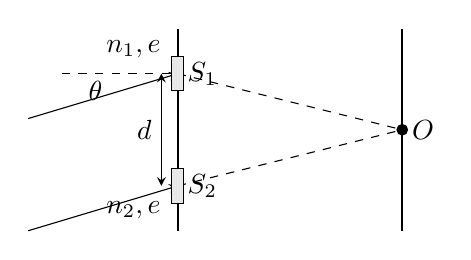
\begin{tikzpicture}[scale=0.95,>=stealth]
  \draw[thick] (0,-1.35) -- (0,1.35);
  \filldraw (0,0.75) circle (2pt) node[right] {\(S_1\)};
  \filldraw (0,-0.75) circle (2pt) node[right] {\(S_2\)};
  \draw[<->] (-0.22,-0.75) -- (-0.22,0.75) node[midway,left] {\(d\)};
  \draw[thick] (3.0,-1.35) -- (3.0,1.35);
  \filldraw (3.0,0) circle (2pt) node[right] {\(O\)};
  \draw[dashed] (0,0.75) -- (3.0,0);
  \draw[dashed] (0,-0.75) -- (3.0,0);
  \draw[->] (-2.0,0.15) -- (0,0.75);
  \draw[->] (-2.0,-1.35) -- (0,-0.75);
  \draw[dashed] (-1.55,0.75) -- (0,0.75);
  \node at (-1.1,0.52) {\(\theta\)};
  \draw[fill=gray!18] (-0.08,0.52) rectangle (0.08,0.98);
  \draw[fill=gray!18] (-0.08,-0.98) rectangle (0.08,-0.52);
  \node[left] at (-0.1,1.08) {\(n_1,e\)};
  \node[left] at (-0.1,-1.08) {\(n_2,e\)};
\end{tikzpicture}
\end{center}
\end{exercise}

\begin{solution}
\textbf{起手判断/模型：} 中央 \(O\) 处的出射几何路程满足 \(S_1O=S_2O\)，所以相位差只来自两件事：斜入射时两缝处入射波本来就有相位差，以及两块介质片带来的附加光程差。

\textbf{主方程：} 先约定
\[
\delta_{12}=L_1-L_2,
\]
即用通过 \(S_1\) 的光路减通过 \(S_2\) 的光路。介质片带来的光程差为
\[
\delta_{\text{film}}=(n_1-n_2)e.
\]
按原图的入射方向，波先到达上缝 \(S_1\)，后到达下缝 \(S_2\)。因此以 \(S_1\) 光路减 \(S_2\) 光路时，斜入射带来的入射端光程差为
\[
\delta_{\text{inc}}=-d\sin\theta.
\]

\textbf{分步代入或化简：} 因此总光程差可写成
\[
\delta_{12}=(n_1-n_2)e-d\sin\theta.
\]
相位差为
\[
\Delta\phi_{12}=\frac{2\pi}{\lambda}\delta_{12}
=\frac{2\pi}{\lambda}\left[(n_1-n_2)e-d\sin\theta\right].
\]

\textbf{结论：}
\[
\boxed{\Delta\phi_{12}=\frac{2\pi}{\lambda}\left[(n_1-n_2)e-d\sin\theta\right]}.
\]

\textbf{物理检查/易错点：} 若题目改成正入射，\(\theta=0\)，结果应退化为两块介质片的相位差；若反过来定义“第二路减第一路”，整个相位差会整体变号，但明暗判据不变。最容易错的是只写 \((n_1-n_2)e\)，漏掉斜入射在两缝处已经造成的相位差。
\end{solution}

\section{光路中插入介质片后条纹怎样移动}

这一节要解决的问题是：为什么在一条光路上插入一片透明介质后，整幅干涉图样会整体平移？

设在上缝 \(S_1\) 后放入折射率为 \(n\)、厚度为 \(e\) 的透明片。若屏上坐标 \(x\) 的正方向取向 \(S_1\) 一侧，则总光程差可写成
\[
\begin{aligned}
\Delta L&=L_2-L_1=(r_2-r_1)-(n-1)e,\\
r_2-r_1&\approx \frac{dx}{D}
\implies
\Delta L\approx \frac{dx}{D}-(n-1)e.
\end{aligned}
\]

\bridge{条纹整体平移的原因就在这里：插入介质片后，\(S_1\) 这一路等效地“落后”了 \((n-1)e\) 这么一段光程，所以原来满足某一级明纹条件的位置必须换到别处去补偿这段落后量。}

于是新的明纹位置满足
\[
\frac{dx_k}{D}-(n-1)e=k\lambda
\implies
x_k=\frac{D}{d}\left[k\lambda+(n-1)e\right],\qquad
x_0=\frac{D(n-1)e}{d}.
\]
这说明：
\begin{itemize}
  \item 整个干涉图样会向\textbf{插入介质片的那一侧}平移；
  \item 条纹间距 \(\Delta x=\lambda D/d\) 保持不变。
\end{itemize}

\begin{note}
\textbf{先看什么信号：} 题目一说“某一路插入介质片”且又问条纹往哪边移，先想到新增的是光程差，不是条纹间距；\textbf{这条公式在控制什么：} \((n-1)e\) 控制的是整幅图样的整体平移量；\textbf{怎样最快记住：} 哪一路被加片，哪一路就等效“落后”，亮纹就整体朝那一路偏；\textbf{最容易错：} 只记移动方向，却忘了 \(\Delta x=\lambda D/d\) 仍由双缝几何决定，插片不会改条纹疏密。
\end{note}

\begin{exercise}[原中央明纹处为什么还能落在某一级明纹上]
双缝干涉中，入射光波长为 \(\lambda\)，双缝至屏距离为 \(D\)。在一个缝后放入厚度为 \(b\)、折射率为 \(n\) 的透明薄片后，原中央明纹处仍为一明纹。求该处对应的干涉级次。
\end{exercise}

\begin{solution}
\textbf{起手判断/模型：} 题目问的是“原中央位置现在属于第几级”，所以第一步不该先去求新中央位置，而应直接在原中央位置记总光程差。

\textbf{主方程：}
\[
\Delta L=(r_2-r_1)-(n-1)b.
\]

\textbf{分步代入或化简：} 原中央明纹处有 \(r_1=r_2\)，故
\[
\Delta L=-(n-1)b.
\]
若该处仍为明纹，则
\[
\Delta L=-k\lambda,\qquad k=0,1,2,\dots
\implies
k=\frac{(n-1)b}{\lambda}.
\]

\textbf{结论：} 原中央明纹处在加片后对应的明纹级次为
\[
\boxed{k=\frac{(n-1)b}{\lambda}}.
\]

\textbf{物理检查/易错点：} 这里的 \(k\) 只是在回答“原中央位置补偿了多少级光程差”，并不等于新的中央明纹编号。最容易错的是把“原中央处仍亮”误解成“图样根本没动”。
\end{solution}

\begin{exercise}[中央明纹上移 3 条时怎样反推介质片厚度]
杨氏双缝实验中，用透明片遮住上缝后，观察到中央明纹向上移动了 3 个条纹。已知透明片折射率 \(n=1.4\)，入射光波长 \(\lambda=0.55\times10^{-6}\,\si{m}\)。求透明片厚度。
\end{exercise}

\begin{solution}
\textbf{起手判断/模型：} “中央明纹移动了 3 个条纹”这句话，应该先翻译成“新增光程差恰好对应 3 个波长”，而不是先去重画整幅条纹图。

\textbf{主方程：}
\[
(n-1)e=3\lambda.
\]

\textbf{分步代入或化简：}
\[
e=\frac{3\lambda}{n-1}
=\frac{3\times0.55\times10^{-6}}{1.4-1}
=4.125\times10^{-6}\,\si{m}.
\]

\textbf{结论：} 透明片厚度为
\[
\boxed{e=4.125\times10^{-6}\,\si{m}}.
\]

\textbf{物理检查/易错点：} 厚度落在微米级，正是干涉测量微小厚度最常见的量级。最容易错的是把新增光程差直接写成 \(ne\)，而忘了原来空气那段也占了一部分路。
\end{solution}

\begin{exercise}[2011级期末：双缝装置浸入透明液体后的级次变化]
在杨氏双缝干涉实验中，设 \(SS_1=SS_2\)，用波长为 \(\lambda\) 的单色光照射双缝 \(S_1,S_2\)，通过空气后在屏 \(E\) 上形成干涉条纹。已知屏上某点 \(P\) 处为第三级明纹。若将整个装置放入某种透明液体中，\(P\) 点变为第四级明纹，求该液体的折射率 \(n\)。

\begin{center}
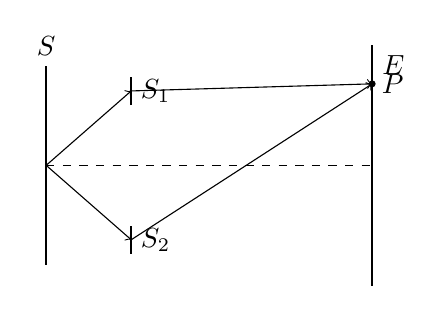
\begin{tikzpicture}[scale=0.9]
  \draw[thick] (0,-1.4) -- (0,1.4) node[above] {\(S\)};
  \draw[thick] (1.2,0.85) -- (1.2,1.25);
  \draw[thick] (1.2,-1.25) -- (1.2,-0.85);
  \node[right] at (1.2,1.05) {\(S_1\)};
  \node[right] at (1.2,-1.05) {\(S_2\)};
  \draw[thick] (4.6,-1.7) -- (4.6,1.7) node[below right] {\(E\)};
  \fill (4.6,1.15) circle (1.4pt) node[right] {\(P\)};
  \draw[->] (0,0) -- (1.2,1.05);
  \draw[->] (0,0) -- (1.2,-1.05);
  \draw[->] (1.2,1.05) -- (4.6,1.15);
  \draw[->] (1.2,-1.05) -- (4.6,1.15);
  \draw[dashed] (0,0) -- (4.6,0);
\end{tikzpicture}
\end{center}
\end{exercise}

\begin{solution}
\textbf{起手判断/模型：} 整个装置浸入液体后，几何路程差 \(\Delta r\) 不变，改变的是光程差：同一段几何路程在液体中要乘上折射率 \(n\)。因此这题不是条纹间距简单缩放，而是同一个屏上点 \(P\) 对应的级次改变。

\textbf{空气中：} \(P\) 为第三级明纹，说明
\[
\Delta r=3\lambda.
\]

\textbf{液体中：} 光程差变为
\[
\Delta L'=n\Delta r.
\]
若 \(P\) 变为第四级明纹，则
\[
n\Delta r=4\lambda.
\]
代入空气中的 \(\Delta r=3\lambda\)，得
\[
3n\lambda=4\lambda
\implies
n=\frac43\approx 1.33.
\]

\textbf{结论：}
\[
\boxed{n\approx 1.33}.
\]

\textbf{物理检查/易错点：} 把装置整体浸入液体时，屏和双缝位置没有改变，所以几何路程差没有变；真正改变的是相位累积速度。也可等价地说液体中波长变为 \(\lambda/n\)，于是同一 \(\Delta r=3\lambda\) 会对应 \(3n\) 个液体中波长。
\end{solution}

\section{干涉题的统一入口}

\begin{itemize}
  \item 先找清楚到底是哪两路光在叠加，并判断它们为什么相干。
  \item 再判断比较的是路程差、光程差，还是总光程差。
  \item 若有反射，必须额外判断是否存在半波损失。
  \item 最后才代入明暗条件、条纹位置公式或光强公式。
\end{itemize}

\section{分波阵面干涉的其他实验}

这一节要解决的问题是：为什么双缝、双棱镜、双面镜、洛埃镜这些装置长相不同，却都属于同一类干涉实验？

它们的共同本质都是：\textbf{把同一原始波前拆成两路等效次波源，再让这两路光重新叠加。}

\subsection{菲涅耳双棱镜与双面镜}

菲涅耳双棱镜利用折射，把来自同一狭缝的光分成两束，等效成两个虚光源；菲涅耳双面镜则利用两面夹角很小的平面镜，把同一光源反射成两个虚像光源。

这两类实验可以统一记成一句话：\textbf{先把一个真实光源变成两个等效虚光源，再让这两个虚光源像双缝那样发生干涉。}

\subsection{洛埃镜}

洛埃镜实验里，一路光直接从光源到屏，另一路光先经镜面反射后再到屏。反射光可以看成来自镜后虚光源，因此也能与直射光发生干涉。

\begin{note}
洛埃镜最重要的考点不是会画图，而是知道：\textbf{反射光相对于直射光会多出半波损失。} 因此靠近镜边的某些本来应当“同程”的位置，反而会出现暗纹。
\end{note}

\begin{exercise}[2007级期末：双缝明纹加高折射率反射面后变暗]
在双缝干涉实验中，屏幕 \(E\) 上 \(P\) 点原来是明条纹。若将缝 \(S_2\) 盖住，并在 \(S_1S_2\) 连线的垂直平分面处放一高折射率介质反射面 \(M\)，如图所示。判断此时 \(P\) 点是明条纹还是暗条纹。

\begin{center}

\includegraphics[width=0.30\linewidth]{pdf-exercises/pdf2007-q07-lloyd-mirror.png}
\end{center}
\end{exercise}

\begin{solution}
\textbf{起手判断/模型：} 反射面放在 \(S_1S_2\) 连线的垂直平分面处，反射光可看成来自 \(S_1\) 关于镜面的虚像，而这个虚像与原来的 \(S_2\) 等效。几何光程关系因此继承了原双缝中 \(S_1,S_2\) 到 \(P\) 的关系。

\textbf{主方程：} 原来 \(P\) 为明纹，说明两缝到 \(P\) 的光程差满足
\[
\Delta L=k\lambda.
\]
现在一路为 \(S_1\) 直达 \(P\)，另一路为 \(S_1\) 经高折射率反射面反射后到 \(P\)。由于反射等效虚源为 \(S_2\)，几何部分仍对应整数倍波长；但从空气侧在高折射率介质表面反射，会产生半波损失，相当于额外相差
\[
\frac{\lambda}{2}.
\]
因此总光程差变为
\[
\Delta L'=k\lambda+\frac{\lambda}{2}
=\left(k+\frac12\right)\lambda.
\]

\textbf{结论：}
\[
\boxed{P\text{ 点变为暗条纹}.}
\]

\textbf{物理检查/易错点：} 本题不是说“盖住一个缝就没有干涉”。反射面提供了第二路相干光；真正改变明暗的是高折射率反射带来的半波损失。
\end{solution}

\section{反射光的相位突变与半波损失}

\textbf{本节问题：} 为什么有些光一反射，明明几何路程没多出半个波长，却还要在干涉总账里额外补一个 \(\lambda/2\)？

\textbf{物理图景：} 关键不在“反射了没有”，而在“反射时电振动有没有翻向”。当光从光疏介质射向光密介质并发生反射时，反射光的电振动相当于整体反号，这就是相位多了 \(\pi\)；而 \(\pi\) 的相位差又恰好等效于半个波长的光程差。于是半波损失并不是另一条独立规定，而只是“反射时翻相”换成光程语言后的记账方式。

\begin{definition}[半波损失]\label{def:half-wave-loss}
光从光疏介质射向光密介质并发生反射时，反射光会发生相位突变 \(\pi\)，等效于额外增加了 \(\lambda/2\) 的附加光程差。这种现象叫做\textbf{半波损失}。
\end{definition}

这里的 \(\lambda\) 按本章统一口径指真空中的波长。

\begin{note}
判断是否有半波损失，一个最稳的办法是：看反射发生时，光是不是从折射率较小的一侧反射到折射率较大的一侧。若是，就发生半波损失；若不是，就没有这项附加的 \(\lambda/2\)。
\end{note}

\begin{remark}
这一节非常关键，因为后面的洛埃镜、薄膜干涉、牛顿环都会反复用到同一条判断线：\textbf{相位是否翻转，等效是不是多了半个波长。}
\end{remark}

\section{薄膜干涉（分振幅法）}

这一节要解决的问题是：同一束光在薄膜上下表面反射之后，为什么会自己和自己发生干涉？

这里第一次最容易误会的是：好像薄膜题只是在比“谁多走了一段路”。其实真正该记的是\textbf{相位总账}。两束光最后能不能同相，不只取决于它们在膜里多走了多少几何路程，还取决于反射时有没有额外翻相，也就是有没有半波损失。薄膜干涉属于分振幅干涉。同一束入射光在薄膜的上、下表面发生部分反射和部分透射，于是分成两束相干光。它们之后重新相遇，便会形成明暗条纹。

常见的肥皂泡彩纹、地面油膜彩纹、光学镀膜，都属于薄膜干涉的应用。

\section{薄膜干涉公式与附加光程差}

设薄膜折射率为 \(n\)，厚度为 \(d\)，光在膜内折射角为 \(r\)。对最常见的平行薄膜模型，两束主要反射光之间的总光程差可写成
\[
\delta=2nd\cos r+\delta_2,
\]
其中
\begin{itemize}
  \item \(2nd\cos r\) 是几何光程差；
  \item \(\delta_2\) 是由反射相位突变带来的附加光程差。
\end{itemize}

\begin{note}
\textbf{先画两束光：} 一束在上表面直接反射回去，另一束先透入薄膜、在下表面反射、再返回上表面射出。后者比前者恰好多走了一次“下去再上来”的膜内路程，所以几何部分写成 \(2nd\cos r\)；若两束光在反射时经历的半波损失次数不同，还要再补上附加光程差 \(\delta_2\)。
\end{note}

\(\delta_2\) 的判断规则可以直接写成：
\begin{itemize}
  \item 若两束参与干涉的光在反射时经历的半波损失次数同为 0 次或同为 1 次，则 \(\delta_2=0\)；
  \item 若一束有半波损失而另一束没有，则 \(\delta_2=\lambda/2\)。
\end{itemize}

当近似垂直入射时，\(\cos r\approx 1\)，公式简化为
\[
\delta\approx 2nd+\delta_2.
\]

\begin{exercise}[上下表面反射光相遇时的相位差]
平行单色光垂直照射到薄膜上，经上下两表面反射的两束光发生干涉。薄膜厚度为 \(e\)，折射率满足 \(n_1<n_2>n_3\)，入射光在折射率为 \(n_1\) 的介质中的波长为 \(\lambda_1\)。求两束反射光在相遇点的相位差。

\begin{center}

\includegraphics[width=0.26\linewidth]{pdf-exercises/pdf2003-q08-film.png}
\end{center}
\end{exercise}

\begin{solution}
\textbf{起手判断/模型：} 垂直入射薄膜题先算膜内往返造成的相位差，再判断两束反射光是否有额外 \(\pi\) 相位差。这里上表面反射是从 \(n_1\) 到 \(n_2\)，有半波损失；下表面反射是从 \(n_2\) 到 \(n_3\)，由于 \(n_2>n_3\)，没有半波损失。因此两束反射光额外相差 \(\pi\)。

\textbf{主方程：} 入射介质中的波长为 \(\lambda_1\)，对应真空波长为
\[
\lambda_0=n_1\lambda_1.
\]
膜内往返光程为 \(2n_2e\)，所以几何相位差为
\[
\Delta\varphi_{\text{geom}}
=\frac{2\pi}{\lambda_0}\,2n_2e
=\frac{4\pi n_2e}{n_1\lambda_1}.
\]

\textbf{结论：} 加上一次半波损失造成的额外 \(\pi\)，总相位差为
\[
\boxed{\Delta\varphi=\frac{4\pi n_2e}{n_1\lambda_1}+\pi}.
\]

\textbf{物理检查/易错点：} 题目给的 \(\lambda_1\) 不是真空波长，而是 \(n_1\) 介质中的波长，所以换算相位时要用 \(\lambda_0=n_1\lambda_1\)。最容易错的是把 \(n_2\lambda_1\) 当成膜内波长，或漏掉一次反射相位突变。
\end{solution}

\begin{exercise}[2011级期末：\(n_1>n_2>n_3\) 薄膜反射光的相位差]
平行单色光垂直入射在折射率为 \(n_2\) 的薄膜上，薄膜上下介质折射率满足
\[
n_1>n_2>n_3.
\]
设薄膜厚度为 \(e\)，入射光在真空中的波长为 \(\lambda\)。求上下两个表面反射的两束光相遇时的相位差。
\end{exercise}

\begin{solution}
\textbf{起手判断/模型：} 这题的重点不是厚度项，而是半波损失次数。上表面反射发生在 \(n_1\to n_2\)，是从光密到光疏反射，没有半波损失；下表面反射发生在 \(n_2\to n_3\)，也是从光密到光疏反射，也没有半波损失。

\textbf{主方程：} 因为两束反射光的反射相位突变相同，附加相位差为零，只剩膜内往返带来的相位差：
\[
\Delta\varphi
=\frac{2\pi}{\lambda}\,(2n_2e)
=\frac{4\pi n_2e}{\lambda}.
\]

\textbf{结论：}
\[
\boxed{\Delta\varphi=\frac{4\pi n_2e}{\lambda}}.
\]

\textbf{物理检查/易错点：} 折射率顺序 \(n_1>n_2>n_3\) 使两次反射都不是“低到高”反射，因此没有额外的 \(\pi\)。若看到薄膜题就机械加 \(\pi\)，会把本题选成另一类答案。
\end{solution}

\begin{note}
\textbf{先看什么信号：} 只要题面出现薄膜、空气隙、镀膜或反射观察，就先把参与干涉的两束光和两次反射分开画清；\textbf{这条公式在控制什么：} \(2nd\cos r\) 控制几何累积，\(\delta_2\) 控制相位是否额外翻半波；\textbf{怎样最快记住：} 薄膜题最稳的顺序永远是“先算几何光程差，再判断附加光程差”；\textbf{最容易错：} 只背最后的明暗条件，不先判断半波损失次数。
\end{note}

\section{薄膜干涉加强与相消条件}

这一节第一次最稳的入口不是背“明暗条件谁和谁对调”，而是先把比较对象锁死：\textbf{你现在看到的是反射光，还是透射光？你的总光程差 \(\delta\) 里，到底有没有把半波损失算进去？} 一旦这两步说清，明暗条件就只是“最终同相还是反相”的直接翻译。

最一般的判据其实很简单：
\[
\delta=k\lambda \implies \text{相长干涉},\qquad
\delta=\left(k+\frac12\right)\lambda \implies \text{相消干涉}.
\]

真正容易混乱的，不是这两句，而是“你的 \(\delta\) 到底已经把半波损失算进去了没有”。

对最常见的“空气---薄膜---基底”模型，若两束反射光之间恰好只有一次半波损失，则反射光总光程差及反射光与透射光的明暗条件可并排记成
\[
\begin{aligned}
\delta_{\text{反}}&=2nd\cos r+\frac{\lambda}{2},\\
\text{反射光:}\quad
&2nd\cos r=\left(k+\frac12\right)\lambda &&\text{明纹},\\
&2nd\cos r=k\lambda &&\text{暗纹};\\[3pt]
\text{透射光:}\quad
&2nd\cos r=k\lambda &&\text{明纹},\\
&2nd\cos r=\left(k+\frac12\right)\lambda &&\text{暗纹}.
\end{aligned}
\]

\begin{exercise}[2008级期末：空气中透明薄膜反射加强的最小厚度]
一束波长为 \(\lambda\) 的单色光由空气垂直入射到折射率为 \(n\) 的透明薄膜上，透明薄膜放在空气中。要使反射光得到干涉加强，求薄膜的最小非零厚度。
\end{exercise}

\begin{solution}
\textbf{起手判断/模型：} 结构是“空气--薄膜--空气”。上表面反射从低折射率到高折射率，有半波损失；下表面反射从高折射率到低折射率，没有半波损失。因此两束反射光之间有一次半波损失。

\textbf{主方程：} 正入射时几何光程差为 \(2nd\)。若把一次半波损失写成附加光程 \(\lambda/2\)，反射加强条件为
\[
2nd+\frac{\lambda}{2}=k\lambda.
\]

\textbf{分步代入或化简：} 求最小非零厚度，取 \(k=1\)，得
\[
2nd=\frac{\lambda}{2}
\implies
d_{\min}=\frac{\lambda}{4n}.
\]

\textbf{结论：}
\[
\boxed{d_{\min}=\frac{\lambda}{4n}}.
\]

\textbf{物理检查/易错点：} 这里是反射加强，不是增透相消。由于只有一次半波损失，反射加强对应 \(2nd=(k+\frac12)\lambda\)，最小值就是四分之一膜内波长。
\end{solution}

\begin{note}
\textbf{先看什么信号：} 题面若明确“反射观察/透射观察”或问中心明暗，就要先确认半波损失是否已计入总光程差；\textbf{这条公式在控制什么：} 上面这组条件控制的是一次半波损失模型下，反射与透射两路何时互为强弱；\textbf{怎样最快记住：} 同一厚度下，反射亮时透射往往暗，反过来也成立；\textbf{最容易错：} 不先说明自己的 \(\delta\) 是否已经含 \(\lambda/2\)，就机械背“反射明纹/暗纹”口号。
\end{note}

\begin{remark}
如果题目条件换了，附加光程差 \(\delta_2\) 也可能跟着变，这时最安全的方法依然是先写总光程差 \(\delta\)，再回到最一般的明暗判据，不要机械硬背“反射明、透射暗”一类简化口号。
\end{remark}

\section{增透膜与增反膜}

薄膜干涉不只是“看条纹”，还是光学镀膜的理论基础。若希望某一目标波长的反射尽量弱，就让反射光相消；若希望反射尽量强，就让反射光相长。

\begin{exercise}[四分之一波长增透膜的最小厚度]
若某一薄膜用于目标波长 \(\lambda\) 的增透设计，并满足常见的一次半波损失条件，求其最小厚度。
\end{exercise}

\begin{solution}
\textbf{起手判断/模型：} “增透膜”四个字已经把模型说死了：目标是让\textbf{反射光尽量相消}，从而把更多光送进透射方向。题目又强调求最小厚度，所以应优先找满足相消条件的最小非零膜厚。

\textbf{主方程：} 对课内最常用的四分之一波长增透膜模型，最省厚度的做法是让膜内往返光程正好多补出半个波长，即
\[
2nd=\frac{\lambda}{2}\implies d_{\min}=\frac{\lambda}{4n}.
\]

\textbf{结论：} 最小厚度为 \(d_{\min}=\dfrac{\lambda}{4n}\)。

\textbf{物理检查/易错点：} 结果随折射率 \(n\) 增大而变薄，符合“同样几何厚度下，折射率越大，相位积累越快”的直觉。最容易错的是一上来只背“增透膜等于四分之一波长”，却说不清这一步实际上是在让两束主要反射光在反射方向上相消。
\end{solution}

\begin{exercise}[2007级期末：MgF2 增透膜的最小厚度]
在玻璃表面镀一层 \(\mathrm{MgF_2}\) 薄膜作为增透膜。空气折射率取 \(1.00\)，\(\mathrm{MgF_2}\) 折射率为 \(1.38\)，玻璃折射率为 \(1.60\)。为使波长 \(\lambda=\SI{500}{nm}\) 的光从空气正入射时尽可能少反射，求 \(\mathrm{MgF_2}\) 薄膜的最小厚度。
\end{exercise}

\begin{solution}
\textbf{起手判断/模型：} 这是反射光相消的增透膜题。空气到薄膜、薄膜到玻璃两个反射都从低折射率侧反射到高折射率侧，所以两束主要反射光都有半波损失，相对附加相位差为零。

\textbf{主方程：} 正入射时，两束反射光的几何光程差为
\[
\delta=2nd.
\]
要让反射尽量相消，最小非零厚度满足
\[
2nd=\frac{\lambda}{2}
\implies d_{\min}=\frac{\lambda}{4n}.
\]

\textbf{分步代入或化简：}
\[
d_{\min}=\frac{500\,\si{nm}}{4\times1.38}
\approx \SI{90.6}{nm}.
\]

\textbf{结论：}
\[
\boxed{d_{\min}\approx\SI{90.6}{nm}}.
\]

\textbf{物理检查/易错点：} 若两次反射的半波损失次数相同，就不要再额外加 \(\lambda/2\)。这里的四分之一波长是膜内光学厚度条件，不是真空中直接取 \(\SI{125}{nm}\)。
\end{solution}

\begin{note}
增透膜与增反膜并不是“新现象”，而只是把同一套薄膜干涉规律用在工程设计里。看到镀膜题时，先问自己：这道题希望反射光相消，还是相长？
\end{note}

\begin{exercise}[油膜上下观察时为什么会看到不同颜色]
一层折射率 \(n_1=1.20\) 的油膜浮在海水表面，海水折射率 \(n_2=1.30\)。若太阳在头顶正上方，某处油膜厚度 \(d=\SI{460}{nm}\)。问从空中向下看时呈什么颜色；若潜水员从水下向上看，又会看到什么主颜色。
\end{exercise}

\begin{solution}
\textbf{起手判断/模型：} 这题最重要的是先分清“从空中看”对应反射观察，“从水下看”对应透射观察。两者不能套同一组明暗条件。

\textbf{主方程：}
\[
\delta_{\text{反}}=2n_1d,\qquad
\delta_{\text{透}}=2n_1d+\frac{\lambda}{2}.
\]

\textbf{分步代入或化简：} 先算
\[
2n_1d=2\times1.20\times460\,\si{nm}=1104\,\si{nm}.
\]
从空中看是反射增强：
\[
2n_1d=k\lambda
\implies
\lambda=\frac{1104}{k}\,\si{nm}.
\]
试可见光范围，最显著的可见解为
\[
k=2\Rightarrow \lambda=552\,\si{nm},
\]
对应绿光。

从水下看是透射增强：
\[
2n_1d+\frac{\lambda}{2}=k\lambda
\implies
\lambda=\frac{1104}{k-\frac12}\,\si{nm}.
\]
试可见光范围得
\[
k=2\Rightarrow \lambda=736\,\si{nm},\qquad
k=3\Rightarrow \lambda=441.6\,\si{nm}.
\]
其中主显著可见颜色可取红光。

\textbf{结论：} 从空中向下看主呈绿色；从水下向上看主呈红色。

\textbf{物理检查/易错点：} 本题最容易错在把上下观察都按反射题处理。真正稳的做法是先问“眼睛接收到的是哪一路光”。
\end{solution}

\section{等厚干涉}

当干涉条纹的形状取决于“薄膜上厚度相同的点的轨迹”时，得到的就是\textbf{等厚干涉}。

若入射角保持不变，则薄膜干涉中的光程差主要由厚度 \(d\) 决定。于是：
\begin{itemize}
  \item 厚度相同的点，光程差相同；
  \item 光程差相同的点，会落在同一条明纹或暗纹上。
\end{itemize}

这就是为什么“等厚线长成什么样，条纹就长成什么样”。若等厚线是直线，条纹就是直线；若等厚线是圆，条纹就是圆环。

\section{劈尖薄膜的干涉}

两块玻璃形成很小夹角时，中间的空气层或透明薄层厚度沿某一方向线性变化，这样的薄膜就叫\textbf{劈尖}。

设劈尖角为 \(\alpha\)，介质折射率为 \(n\)。在小角近似下，若从棱边起沿垂直于棱边方向量坐标 \(x\)，则薄膜厚度近似满足 \(d\approx \alpha x\)。

在最常见的反射观察模型里，劈尖等厚条纹是一些\textbf{与棱边平行的明暗相间直条纹}。若存在一次半波损失，则在棱边 \(d=0\) 处会首先出现暗纹。

相邻两条亮纹或相邻两条暗纹之间的厚度差都满足
\[
\Delta d=\frac{\lambda}{2n}
\implies
\Delta x=\frac{\lambda}{2n\alpha}.
\]

\begin{note}
\textbf{先看什么信号：} 题目若给出劈尖角、棱边位置和条纹疏密，就先把厚度写成 \(d\approx \alpha x\)；\textbf{这条公式在控制什么：} \(\Delta d=\lambda/(2n)\) 控制相邻同类条纹对应的厚度增量，\(\Delta x=\lambda/(2n\alpha)\) 则把它换成屏上的空间间距；\textbf{怎样最快记住：} 劈尖角越大，厚度随 \(x\) 增长越快，所以同样一份厚度差会在更短距离里出现，条纹就更密；\textbf{最容易错：} 把“等厚条纹”的厚度差和屏上坐标差混为一谈，或者漏掉介质折射率 \(n\)。
\end{note}

\begin{remark}
这个公式直接告诉我们：
\begin{itemize}
  \item 劈尖角越大，条纹越密；
  \item 波长越大，条纹越疏；
  \item 条纹过密时，实验上会难以分辨。
\end{itemize}
\end{remark}

\begin{exercise}[2014级期末：滚柱间距变小时劈尖条纹数和间距怎样变]
两根直径有微小差别、彼此平行的滚柱之间距离为 \(L\)，其上放两块平板玻璃，中间形成空气劈尖。单色光垂直入射时产生等厚干涉条纹。若滚柱之间的距离 \(L\) 变小，判断在两滚柱之间观察到的条纹数和条纹间距怎样变化。
\end{exercise}

\begin{solution}
\textbf{起手判断/模型：} 两滚柱直径差给定，所以两端的空气膜厚度差 \(\Delta d\) 不变；改变 \(L\) 只是改变劈尖角。

\textbf{主方程：} 劈尖角小量近似为
\[
\alpha\approx\frac{\Delta d}{L}.
\]
相邻同类条纹间距为
\[
\Delta x=\frac{\lambda}{2\alpha}
=\frac{\lambda L}{2\Delta d}.
\]
两滚柱之间的总条纹数由总厚度差决定：
\[
N\approx\frac{\Delta d}{\lambda/2}
=\frac{2\Delta d}{\lambda}.
\]

\textbf{结论：} 当 \(L\) 变小时，\(\Delta d\) 不变，所以
\[
\boxed{N\text{ 不变},\qquad \Delta x\text{ 变小}}.
\]

\textbf{物理检查/易错点：} 条纹数看总厚度差，条纹间距看厚度随位置变化的斜率。把两者混在一起，就会误以为间距变小必然让条纹数增加。
\end{solution}

\begin{exercise}[2006级期末：空气劈形膜上玻璃平移时条纹怎样动]
两块平玻璃构成空气劈形膜，左边为棱边，用单色平行光垂直入射。若上面的平玻璃慢慢地向上平移，判断干涉条纹的移动方向和条纹间隔变化。
\end{exercise}

\begin{solution}
\textbf{起手判断/模型：} 劈尖条纹是等厚线。上玻璃若整体向上平移，劈尖角不变，因此厚度随位置的斜率不变；但每个位置的空气膜厚度都会增加同一个常量。

\textbf{主方程：} 设平移前空气膜厚度近似为
\[
d(x)=\alpha x.
\]
上板整体上移 \(h\) 后变为
\[
d'(x)=h+\alpha x.
\]
某一条同级条纹要求膜厚等于固定值 \(d_k\)，因此新位置满足
\[
h+\alpha x'=d_k,\qquad \alpha x=d_k.
\]
于是
\[
x'=x-\frac{h}{\alpha}.
\]

\textbf{结论：}
\[
\boxed{\text{条纹向棱边方向平移，条纹间隔不变}.}
\]

\textbf{物理检查/易错点：} 条纹间隔由斜率 \(\alpha\) 决定；平移只给厚度加常量，不改斜率，所以间隔不变。最容易错的是把“厚度增加”误判成“劈尖角变大”。
\end{solution}

\section{劈尖条纹的移动与微小厚度测量}

劈尖干涉最重要的实验价值之一，就是把“极小的厚度变化”放大成“看得见的条纹移动”。

\textbf{第一类：测细丝直径或薄膜厚度。} 若把一根细丝夹在两块玻璃之间形成劈尖，测得棱边到细丝的距离为 \(L\)，相邻条纹间距为 \(l\)，则由
\[
\alpha=\frac{D}{L},\qquad
l=\frac{\lambda}{2n\alpha}
\implies
D=L\alpha=\frac{L\lambda}{2nl}.
\]

\textbf{第二类：测微小厚度改变量。} 若劈尖角 \(\alpha\) 不变，而某处整体厚度增加了 \(H\)，则整个图样会向\textbf{干涉级次更低的方向}移动，也就是向棱边移动。若条纹总共平移了 \(N\) 个条纹间距，则
\[
H=\frac{N\lambda}{2n},\qquad
N=\frac{A}{l}
\implies
H=\frac{\lambda A}{2nl}.
\]

\begin{note}
“向低级次方向移动”这句话可以这样理解：厚度变大后，原来较低级次条纹所在的位置，现在要由较高级次条纹去补位，于是整幅图样看起来就朝棱边挪过去了。
\end{note}

\begin{exercise}[2008级期末：空气劈尖第四条明纹随劈尖角改变的位移]
用波长为 \(\lambda\) 的单色光垂直照射由两块平玻璃板构成的空气劈形膜，已知劈尖角为 \(\theta\)。若劈尖角变为 \(\theta'\)，求从劈棱数起的第四条明条纹位移值 \(\Delta x\)。
\end{exercise}

\begin{solution}
\textbf{起手判断/模型：} 空气劈尖在反射光中有一次半波损失。距离劈棱 \(x\) 处膜厚近似为 \(d=x\theta\)，反射明纹满足总光程差为整数倍波长。

\textbf{主方程：} 第四条明纹对应
\[
2x_4\theta+\frac{\lambda}{2}=4\lambda.
\]
因此
\[
x_4=\frac{7\lambda}{4\theta}.
\]
当劈尖角变为 \(\theta'\) 时，
\[
x_4'=\frac{7\lambda}{4\theta'}.
\]

\textbf{分步代入或化简：} 位移按新位置减旧位置记：
\[
\Delta x=x_4'-x_4
=\frac{7\lambda}{4}\left(\frac{1}{\theta'}-\frac{1}{\theta}\right)
=\frac{7\lambda(\theta-\theta')}{4\theta\theta'}.
\]

\textbf{结论：}
\[
\boxed{\Delta x=\frac{7\lambda(\theta-\theta')}{4\theta\theta'}}.
\]

\textbf{物理检查/易错点：} 第四条明纹离棱边不是 \(4\) 个条纹间距，而是 \(3.5\) 个条纹间距，因为反射光在棱边处为暗纹。若 \(\theta'\) 变小，条纹间距变大，第四明纹应向远离棱边方向移动，公式也给出正位移。
\end{solution}

\begin{exercise}[第五条暗纹对应的膜厚为什么先从棱边明暗判起]
波长为 \(\lambda\) 的单色光垂直照射到折射率为 \(n_2\) 的劈尖薄膜上，设上下介质折射率满足 \(n_1<n_2<n_3\)。从交棱 \(O\) 开始向右数，表面出现第 \(5\) 条暗纹。求该处膜厚。
\end{exercise}

\begin{solution}
\textbf{起手判断/模型：} 先别急着数“第五条暗纹”对应哪个 \(k\)。最稳的第一步是先判断棱边 \(d=0\) 处到底是明还是暗。由于这里是典型的一次半波损失模型，棱边处会先出现\textbf{明纹}，因此沿右侧数过去时，第 \(1\) 条暗纹对应的是 \(k=0\)。

\textbf{主方程：} 在一次半波损失下，反射暗纹条件写成
\[
2n_2d=\left(k+\frac12\right)\lambda,\qquad k=0,1,2,\dots
\]

\textbf{分步代入或化简：} 因为第 \(1\) 条暗纹对应 \(k=0\)，所以第 \(5\) 条暗纹对应
\[
k=4.
\]
代入暗纹条件：
\[
2n_2d=\left(4+\frac12\right)\lambda=\frac{9}{2}\lambda
\implies
d=\frac{9\lambda}{4n_2}.
\]

\textbf{结论：}
\[
\boxed{d=\frac{9\lambda}{4n_2}}.
\]

\textbf{物理检查/易错点：} 这题最容易错在把“第 \(5\) 条暗纹”机械写成 \(k=5\)。等厚干涉里一定先把\textbf{棱边从哪一种条纹起数}说清楚，再编号。
\end{solution}

\begin{exercise}[用劈尖条纹间距测金属细丝直径时为什么先写几何斜率]
把金属细丝夹在两块平玻璃之间形成空气劈尖。用波长 \(\lambda=\SI{589.3}{nm}\) 的单色光垂直照射，已知金属丝到劈尖顶点的距离 \(L=\SI{28.880}{mm}\)，测得 \(30\) 条明纹跨越的总长度为 \(\SI{4.295}{mm}\)。求金属细丝直径 \(D\)。
\end{exercise}

\begin{solution}
\textbf{起手判断/模型：} 这类题看上去在测长度，其实真正先写的是“厚度沿长度方向怎样线性增长”。也就是说，第一步要把劈尖的几何斜率写成
\[
\alpha\approx \frac{D}{L},
\]
再用条纹间距把 \(\alpha\) 反推出去。

\textbf{主方程：}
\[
l=\frac{\lambda}{2\alpha},\qquad \alpha\approx \frac{D}{L}.
\]
这里空气劈尖取 \(n=1\)。

\textbf{分步代入或化简：} \(30\) 条明纹跨越 \(29\) 个条纹间距，所以
\[
l=\frac{4.295}{29}\,\si{mm}\approx \SI{0.1481}{mm}.
\]
于是
\[
D=L\alpha=L\frac{\lambda}{2l}
=\frac{28.880\times 589.3\times10^{-6}}{2\times0.1481}\,\si{mm}
\approx \SI{0.0574}{mm}.
\]

\textbf{结论：}
\[
\boxed{D\approx \SI{5.74e-2}{mm}= \SI{57.4}{\micro m}}.
\]

\textbf{物理检查/易错点：} 细丝直径落在几十微米量级是合理的。最容易错的地方有两个：一是把 \(30\) 条条纹误当成 \(30\) 个间距，二是漏掉空气层对应 \(n=1\)。
\end{solution}

\section{牛顿环}

这一节第一次真正要做的，不是背 \(r_k^2=kR\lambda\)，而是先把两次“翻译”做对：\textbf{先把透镜几何形状翻成空气膜厚度 \(d(r)\)，再把厚度 \(d\) 翻成干涉明暗条件。} 牛顿环看起来是圆环题，本质上仍然只是薄膜干涉题。

把平凸透镜放在平板玻璃上，中间形成厚度从中心向外逐渐增大的空气薄膜。相同厚度的点构成圆周，所以干涉图样呈同心圆环，这就是\textbf{牛顿环}。

设透镜曲率半径为 \(R\)，距接触点半径为 \(r\) 处的膜厚为 \(d\)。先从几何关系出发：
\[
\begin{aligned}
R^2&=(R-d)^2+r^2\\
\implies d&=R-\sqrt{R^2-r^2}\approx \frac{r^2}{2R}\qquad (r\ll R).
\end{aligned}
\]
这一步非常关键，因为它说明牛顿环里真正与位置成正比的不是 \(r\)，而是 \(r^2\)。

在反射光中观察时，中心处因为存在半波损失而通常是\textbf{暗点}；在透射光中观察时，中心通常是\textbf{亮点}。

先用反射薄膜干涉的明暗条件确定 \(d\) 应满足什么关系，再把 \(d\approx r^2/(2R)\) 代进去，半径公式才会出来。

对反射暗环，常用关系为
\[
\begin{aligned}
\text{反射暗环:}\quad &r_k^2=kR\lambda,\qquad k=0,1,2,\dots\\
\text{反射明环:}\quad &r_k^2=\left(k-\frac12\right)R\lambda,\qquad k=1,2,3,\dots
\end{aligned}
\]

\begin{note}
\textbf{先看什么信号：} 题面只要出现“中心明暗、圆环半径、曲率半径”，先判断看的是反射还是透射；\textbf{这条公式在控制什么：} 牛顿环里真正随位置线性变化的是 \(r^2\)，不是 \(r\) 本身；\textbf{怎样最快记住：} 先用 \(d\approx r^2/(2R)\) 把几何厚度换成半径平方，再接明暗条件；\textbf{最容易错：} 把中心反射暗、透射亮混反，或直接拿半径相减而忘了公式天然落在 \(r^2\) 上。
\end{note}

\begin{remark}
牛顿环有一个很重要的读图特点：越往外走，环与环之间的距离会越来越小，所以图样通常表现为“中间疏，边缘密”。
\end{remark}

\section{牛顿环的应用}

牛顿环最常见的三类应用是：
\begin{itemize}
  \item 测透镜曲率半径；
  \item 检查光学元件表面质量；
  \item 观察油膜或薄层厚度变化引起的条纹变化。
\end{itemize}

\begin{exercise}[牛顿环测曲率半径]
在牛顿环实验中，已知单色光波长为 \(\lambda\)，测得第 \(k\) 个暗环半径为 \(r_k\)，第 \(k+m\) 个暗环半径为 \(r_{k+m}\)。求平凸透镜的曲率半径 \(R\)。
\end{exercise}

\begin{solution}
\textbf{起手判断/模型：} 题目给的是两个\textbf{暗环半径}，目标是求曲率半径 \(R\)。因此第一条方程不该从几何厚度 \(d\) 重新推起，而应直接调用反射暗环关系；两式相减的目的，是把未知级次 \(k\) 消掉，于是
\[
\begin{aligned}
r_k^2&=kR\lambda,\qquad r_{k+m}^2=(k+m)R\lambda,\\
r_{k+m}^2-r_k^2&=(k+m)R\lambda-kR\lambda=mR\lambda
\implies
R=\frac{r_{k+m}^2-r_k^2}{m\lambda}.
\end{aligned}
\]

\textbf{结论：} 平凸透镜的曲率半径为 \(R=\dfrac{r_{k+m}^2-r_k^2}{m\lambda}\)。

\textbf{物理检查/易错点：} \(r^2/\lambda\) 的量纲是长度，和 \(R\) 一致。用平方差而不用半径直接相减的好处，就是不必纠缠中心究竟记作第零级还是第一级；只要两条都是暗环，同一条公式就成立。
\end{solution}

\begin{exercise}[空气换成液体后牛顿环半径怎样反推折射率]
平凸透镜顶点和平板玻璃接触，用单色光垂直照射，观察反射光形成的牛顿环。测得中央暗斑外第 \(k\) 个暗环在空气中半径为 \(r_1\)。若将透镜和玻璃板之间的空气换成某种液体，且液体折射率小于玻璃折射率，第 \(k\) 个暗环半径变为 \(r_2\)。求该液体折射率。
\end{exercise}

\begin{solution}
\textbf{起手判断/模型：} 同一个第 \(k\) 个暗环，对应的是同一级干涉条件；换液体后改变的是薄膜折射率，几何关系 \(d\approx r^2/(2R)\) 不变。

\textbf{主方程：} 反射暗环条件可写成
\[
2nd=k\lambda.
\]
又有
\[
d=\frac{r^2}{2R}.
\]

\textbf{分步代入或化简：} 空气中 \(n\approx1\)，所以
\[
2\cdot 1\cdot \frac{r_1^2}{2R}=k\lambda
\implies
r_1^2=kR\lambda.
\]
换成液体后，
\[
2n\frac{r_2^2}{2R}=k\lambda
\implies
nr_2^2=kR\lambda.
\]
两式相除得
\[
n=\frac{r_1^2}{r_2^2}.
\]

\textbf{结论：}
\[
\boxed{n=\frac{r_1^2}{r_2^2}}.
\]

\textbf{物理检查/易错点：} 液体折射率 \(n>1\) 时，同一级暗环需要更小几何厚度，因此 \(r_2<r_1\)，于是 \(r_1^2/r_2^2>1\)，方向合理。最容易错的是忘记牛顿环公式天然是半径平方关系。
\end{solution}

\begin{exercise}[2011级期末：浸入液体的牛顿环中心暗斑]
平凸透镜与平板玻璃构成牛顿环装置，整个装置浸入折射率为 \(n=\num{1.60}\) 的液体中。平凸透镜折射率为 \(\num{1.68}\)，平板玻璃折射率为 \(\num{1.58}\)。凸透镜可沿轴线 \(OO'\) 上下移动，用波长 \(\lambda=\SI{500}{nm}\) 的单色光垂直入射，从上方观察反射光。若调节后看到中心为暗斑，求凸透镜顶点到平板玻璃的最小距离。

\begin{center}
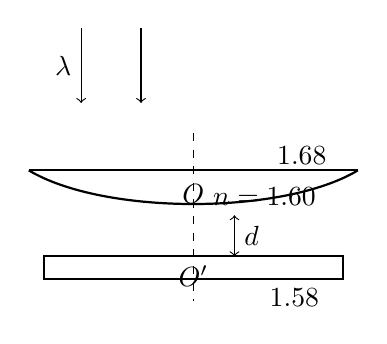
\begin{tikzpicture}[scale=0.95]
  \draw[->] (-1.5,2.6) -- (-1.5,1.6) node[midway,left] {\(\lambda\)};
  \draw[->] (-0.7,2.6) -- (-0.7,1.6);
  \draw[thick] (-2.2,0.7) .. controls (-1.2,0.1) and (1.2,0.1) .. (2.2,0.7);
  \draw[thick] (-2.2,0.7) -- (2.2,0.7);
  \draw[thick] (-2.0,-0.45) rectangle (2.0,-0.75);
  \draw[dashed] (0,1.2) -- (0,-1.05);
  \draw[<->] (0.55,0.10) -- (0.55,-0.45) node[midway,right] {\(d\)};
  \node at (0.95,0.35) {\(n=1.60\)};
  \node at (1.45,0.9) {\(1.68\)};
  \node at (1.35,-1.0) {\(1.58\)};
  \node[above] at (0,0.12) {\(O\)};
  \node[below] at (0,-0.45) {\(O'\)};
\end{tikzpicture}
\end{center}
\end{exercise}

\begin{solution}
\textbf{起手判断/模型：} 这是牛顿环中心明暗问题，中心处的空气膜换成了液体膜，且透镜和玻璃板不一定接触。先判断半波损失，再用中心膜厚 \(d\) 决定两束反射光的相位差。

\textbf{半波损失判断：} 上表面反射发生在透镜到液体界面，折射率从 \(\num{1.68}\) 到 \(\num{1.60}\)，是从光密到光疏反射，没有半波损失；下表面反射发生在液体到平板玻璃界面，折射率从 \(\num{1.60}\) 到 \(\num{1.58}\)，仍是从光密到光疏反射，也没有半波损失。

\textbf{暗斑条件：} 两次反射没有相对的 \(\pi\) 相位突变，所以中心反射光要相消，液体膜内往返光程差需满足
\[
2nd=\left(k+\frac12\right)\lambda,\qquad k=0,1,2,\dots
\]
求最小距离，取 \(k=0\)，得
\[
d_{\min}=\frac{\lambda}{4n}
=\frac{\SI{500}{nm}}{4\times1.60}
=\SI{78.125}{nm}.
\]

\textbf{结论：}
\[
\boxed{d_{\min}\approx \SI{78.1}{nm}}.
\]

\textbf{物理检查/易错点：} 如果中心两面相接 \(d=0\)，因为两次反射都没有相对半波损失，中心应为亮而不是暗。要让中心变暗，最小厚度正是液体中四分之一波长对应的几何厚度 \(\lambda/(4n)\)。本题最容易错的是只凭“牛顿环中心常暗”直接选 \(0\)，却忽略了三种介质的折射率顺序。
\end{solution}

\begin{exercise}[圆形油膜条纹为什么会一圈圈向中心数]
在平面玻璃片上放一油滴并展开成圆形油膜。已知单色光波长 \(\lambda=\SI{600}{nm}\)，玻璃折射率 \(n_1=1.50\)，油膜折射率 \(n_2=1.20\)，油膜中心最高点厚度 \(h=8.0\times10^2\,\si{nm}\)。问：反射观察时条纹如何分布，可见明纹有几条，各明纹处膜厚各是多少；若油膜继续展开，条纹怎样变化？
\end{exercise}

\begin{solution}
\textbf{起手判断/模型：} 这题虽然外形像“圆膜”，但本质仍是等厚干涉。第一步要先认出：油膜厚度从中心向边缘单调减小，所以\textbf{相同厚度对应同心圆}，条纹自然是一圈圈的圆环。又因为这里讨论反射观察，最稳的做法是直接写反射明纹条件。

\textbf{主方程：}
\[
2n_2d=k\lambda,\qquad k=0,1,2,\dots
\]

\textbf{分步代入或化简：} 明纹对应的膜厚为
\[
d_k=\frac{k\lambda}{2n_2}.
\]
代入 \(\lambda=\SI{600}{nm}, n_2=1.20\)，得
\[
d_k=\frac{k\times 600}{2\times1.20}\,\si{nm}=250k\,\si{nm}.
\]
于是
\[
d_0=0,\quad d_1=\SI{250}{nm},\quad d_2=\SI{500}{nm},\quad d_3=\SI{750}{nm},\quad d_4=\SI{1000}{nm}.
\]
由于油膜中心最高厚度只有
\[
h=\SI{800}{nm},
\]
所以能实际出现的明纹厚度只能满足 \(d_k\le h\)。因此可见明纹共有
\[
k=0,1,2,3
\]
这 \(4\) 条。

\textbf{结论：} 反射观察时条纹为同心圆明纹；可见明纹共 \(4\) 条，对应膜厚分别为
\[
0,\ \SI{250}{nm},\ \SI{500}{nm},\ \SI{750}{nm}.
\]
若油膜继续展开，整体厚度减小，则可见条纹数会减少，且相邻条纹间距会变大。

\textbf{物理检查/易错点：} 这题最容易错在把中心最大厚度 \(\SI{800}{nm}\) 也硬凑成一条明纹。真正该做的是先列允许的明纹厚度，再看哪些厚度还塞得进当前油膜。
\end{solution}

\begin{exercise}[空气劈尖条纹弯向薄端时怎样判断凸凹缺陷]
光学平板玻璃 \(A\) 与待测工件 \(B\) 间形成空气劈尖，用波长 \(\lambda=\SI{500}{nm}\) 的单色光垂直照射。反射光干涉条纹如图所示，弯曲部分顶点恰好与其右边相邻直条纹的连线相切。判断工件上表面缺陷是凸起还是凹槽，并求最大高度或深度。

\begin{center}

\includegraphics[width=0.28\linewidth]{pdf-exercises/pdf2004-q09-wedge-defect.png}
\end{center}
\end{exercise}

\begin{solution}
\textbf{起手判断/模型：} 空气劈尖反射条纹是等厚线。条纹向哪边弯，表示相同厚度的位置被缺陷推到了哪里。图中弯曲顶点向劈尖薄端一侧偏移，说明该处空气膜厚度比周围同位置更大，因此工件表面在该处为凸起。

\textbf{厚度判断：} 反射等厚条纹相邻条纹对应的空气膜厚度差为
\[
\Delta d=\frac{\lambda}{2}.
\]
题目说弯曲顶点恰好与右边相邻直条纹相切，表示缺陷导致的最大膜厚变化正好相当于相邻一级条纹，即
\[
h_{\max}=\frac{\lambda}{2}
=\frac{\SI{500}{nm}}{2}
=\SI{250}{nm}.
\]

\textbf{结论：}
\[
\boxed{\text{缺陷为凸起纹，最大高度为 }\SI{250}{nm}}.
\]

\textbf{物理检查/易错点：} 空气劈尖里条纹间隔对应的是膜厚变化 \(\lambda/2\)，不是 \(\lambda\)。最容易错的是只看“弯了一格”就把高度写成 \(\lambda\)。
\end{solution}

\begin{exercise}[2009级期末：劈尖条纹贴近左邻条纹时判断表面缺陷]
用劈尖干涉法检测工件表面缺陷。波长为 \(\lambda\) 的单色平行光垂直入射时，观察到的干涉条纹如图所示：每一条纹弯曲部分的顶点恰好与其左边条纹的直线部分连线相切。判断工件表面在条纹弯曲处对应的部分是凸起还是凹陷，并求最大高度或深度。

\begin{center}

\includegraphics[width=0.25\linewidth]{pdf-exercises/pdf2009-q10-wedge-defect.png}
\end{center}
\end{exercise}

\begin{solution}
\textbf{起手判断/模型：} 空气劈尖反射条纹是等厚线。题图中弯曲顶点向左边相邻条纹靠拢，相当于同一级条纹被推向劈尖薄端。这说明在同一几何位置处空气膜实际变厚了；而空气膜的下表面是工件，所以空气膜变厚对应工件表面局部向下凹陷。

\textbf{厚度方向判断：} 若工件表面局部凹陷，空气层厚度增加。为了重新满足原来那一级等厚条件，条纹位置就要向膜厚较小的一侧移动，也就是向薄端弯曲。题图正是这种情况，所以缺陷为凹陷。

\textbf{大小计算：} 弯曲顶点恰好和相邻直条纹相切，表示最大膜厚变化正好对应一条同级条纹间隔。空气劈尖相邻同类条纹对应的膜厚差为
\[
\Delta d=\frac{\lambda}{2}.
\]
因此缺陷最大高度或深度为
\[
h=\frac{\lambda}{2}.
\]

\textbf{结论：}
\[
\boxed{\text{工件表面凹陷，深度 }h=\frac{\lambda}{2}}.
\]

\textbf{物理检查/易错点：} 判断凸凹时不能只背“向左就是凸、向右就是凹”，必须先看劈尖薄端和厚端在哪一侧。数值上则要记住条纹移动一条，对应空气膜厚度变化 \(\lambda/2\)。
\end{solution}

\begin{exercise}[两种波长第五个牛顿环明环对应膜厚差]
平凸透镜凸面朝下放在平玻璃板上，透镜刚好与玻璃板接触。波长分别为 \(\lambda_1=\SI{600}{nm}\)、\(\lambda_2=\SI{500}{nm}\) 的两种单色光垂直入射，观察反射光形成的牛顿环。求从中心向外数的两种光的第五个明环所对应的空气膜厚度之差。
\end{exercise}

\begin{solution}
\textbf{起手判断/模型：} 反射牛顿环中心为暗，明环条件要带半级差。题目问的是膜厚差，不需要再把膜厚换成半径。

\textbf{主方程：} 反射明环满足
\[
2d=\left(k-\frac12\right)\lambda,\qquad k=1,2,3,\dots
\]
第五个明环对应 \(k=5\)，故
\[
d=\frac{k-\frac12}{2}\lambda
=\frac{9}{4}\lambda.
\]

\textbf{分步代入或化简：}
\[
\Delta d=\frac94(\lambda_1-\lambda_2)
=\frac94(600-500)\,\si{nm}
=\SI{225}{nm}.
\]

\textbf{结论：}
\[
\boxed{\Delta d=\SI{225}{nm}}.
\]

\textbf{物理检查/易错点：} 第五个明环不是 \(2d=5\lambda\)，而是 \(2d=(5-\frac12)\lambda\)。中心暗点会把明环条件整体错开半级。
\end{solution}

\begin{remark}
若拿标准光学面和待检曲面轻轻贴合，若没有牛顿环，说明两者曲率非常匹配；若出现牛顿环，则说明两者曲率仍有差异。于是牛顿环也能用来检验元件表面质量。
\end{remark}

\section{迈克耳孙干涉仪}

迈克耳孙干涉仪属于典型的分振幅干涉装置。它把同一束光在分光板处分成两束，让它们分别走两条完全分开的路径、再返回叠加。

它最重要的装置特点有三条：
\begin{itemize}
  \item 两路相干光在空间上完全分开，因此便于单独调节其中一路；
  \item 可通过移动反射镜或在某一路中插入介质片，极精细地改变光程差；
  \item 补偿板的作用，是让两束光穿过的玻璃厚度尽可能对称，从而避免多余光程差干扰。
\end{itemize}

若把其中一个反射镜平移 \(\Delta d\)，由于光要往返一次，该路光程差改变
\[
\Delta L=2\Delta d,\qquad
2\Delta d=N\lambda
\implies
\Delta d=\frac{N\lambda}{2}.
\]

\begin{note}
\textbf{先看什么信号：} 题目一旦给“镜面移动量”和“移过多少条条纹”，第一条方程就该落到 \(2\Delta d=N\lambda\)；\textbf{这条公式在控制什么：} 它控制的是镜子平移如何转成往返光程差变化；\textbf{怎样最快记住：} 镜子只挪一次，光却要来回走两次，所以光程差总是多一个系数 \(2\)；\textbf{最容易错：} 忘了往返程，把 \(\Delta d\) 直接当成 \(\Delta L\)。
\end{note}

迈克耳孙干涉仪还常出现两类图样：\textbf{等倾干涉}和\textbf{等厚干涉}。它们只是同一装置在不同几何条件下表现出的不同条纹家族。

\begin{remark}
迈克耳孙-莫雷实验的“零结果”宣告了经典以太模型行不通，这一点在物理史上非常重要。不过本章把重点放在装置的干涉原理和条纹计数关系上即可。
\end{remark}

\begin{exercise}[2005级期末：迈克耳孙干涉仪中插入薄膜的厚度]
在迈克耳孙干涉仪的一支光路中，放入一片折射率为 \(n\) 的透明介质薄膜后，测出两束光的光程差改变量为一个波长 \(\lambda\)。求薄膜厚度。
\end{exercise}

\begin{solution}
\textbf{起手判断/模型：} 迈克耳孙干涉仪中一支光路要往返一次。插入薄膜后，空气段被介质段替代，单程附加光程为 \((n-1)d\)，往返后要乘 \(2\)。

\textbf{主方程：}
\[
\Delta L=2(n-1)d.
\]

\textbf{分步代入或化简：} 题目给出光程差改变量为一个波长：
\[
2(n-1)d=\lambda
\implies
d=\frac{\lambda}{2(n-1)}.
\]

\textbf{结论：}
\[
\boxed{d=\frac{\lambda}{2(n-1)}}.
\]

\textbf{物理检查/易错点：} 最容易漏掉迈克耳孙装置的往返程，把附加光程误写成 \((n-1)d\)。这里的 \(n-1\) 也说明我们比较的是“介质替代空气”带来的附加光程，而不是单纯的 \(nd\)。
\end{solution}

\begin{exercise}[2005级期末：双缝中一缝覆云母片后中央明纹移动]
在双缝干涉实验中，若把一厚度为 \(e\)、折射率为 \(n\) 的薄云母片覆盖在 \(S_1\) 缝上，如图所示。判断中央明条纹移动方向，并求两束相干光至原中央明纹 \(O\) 处的光程差。

\begin{center}

\includegraphics[width=0.28\linewidth]{pdf-exercises/pdf2005-q17-mica-double-slit.png}
\end{center}
\end{exercise}

\begin{solution}
\textbf{起手判断/模型：} 云母片只放在 \(S_1\) 后，相当于让 \(S_1\) 这一路额外增加光程 \((n-1)e\)。条纹会向被加片的一侧移动，因为新的中央明纹要跑到能补偿这段附加光程的位置。

\textbf{主方程：}
\[
\Delta L_{\text{片}}=(n-1)e.
\]

\textbf{分步代入或化简：} 在原中央明纹 \(O\) 处，未加片时两缝到 \(O\) 的几何路程相等。加片后 \(S_1\) 路光程多出
\[
(n-1)e.
\]
若按“\(S_1\) 路相对 \(S_2\) 路”的光程差记，则原 \(O\) 处光程差为
\[
\Delta L=(n-1)e.
\]
为了重新使两路同相，中央明纹需向 \(S_1\) 一侧移动；图中 \(S_1\) 在上方，因此中央明纹向上移动。

\textbf{结论：}
\[
\boxed{\text{中央明条纹向上移动}},\qquad
\boxed{\Delta L=(n-1)e}.
\]

\textbf{物理检查/易错点：} 条纹移动方向常被背反。稳妥的判断是：哪一路被加片，哪一路光程变长；新的中央明纹就向那一路所在的一侧移动，以用几何路程差把它补回来。
\end{solution}

\begin{exercise}[2008级期末：双缝一缝加玻璃纸后原明纹变暗]
在双缝干涉实验中，入射光波长为 \(\lambda\)。用玻璃纸遮住双缝中的一个缝，若玻璃纸中光程比相同厚度空气的光程大 \(2.5\lambda\)，判断屏上原来的明纹处变成明纹还是暗纹。
\end{exercise}

\begin{solution}
\textbf{起手判断/模型：} 原来的明纹处说明两路光到该点的光程差为整数倍波长。现在只在其中一路插入玻璃纸，相当于额外增加一段光程差。

\textbf{主方程：}
\[
\Delta L_{\text{原}}=k\lambda,\qquad
\Delta L_{\text{附加}}=2.5\lambda.
\]

\textbf{分步代入或化简：} 新的总光程差为
\[
\Delta L
=k\lambda+2.5\lambda
=\left(k+2+\frac12\right)\lambda.
\]
它比整数倍波长多出半个波长，因此两束光在原明纹处变为反相。

\textbf{结论：}
\[
\boxed{\text{屏上原来的明纹处变为暗纹}}.
\]

\textbf{物理检查/易错点：} 额外光程差 \(2.5\lambda\) 不是“两个半波长所以仍是明纹”，而是“两个整波长再加半波长”。真正决定明暗的是去掉整数倍后剩下的半波长。
\end{solution}

\begin{exercise}[2005级期末：牛顿环透镜上移时移过固定点的条纹数]
用波长为 \(\lambda\) 的单色光垂直照射牛顿环装置，观察从空气膜上下表面反射的光形成的牛顿环。若使平凸透镜从顶点与平面玻璃接触开始，慢慢垂直向上移动到两者距离为 \(d\)，求移过视场中某固定观察点的条纹数目。

\begin{center}

\includegraphics[width=0.24\linewidth]{pdf-exercises/pdf2005-q18-newton-ring-lift.png}
\end{center}
\end{exercise}

\begin{solution}
\textbf{起手判断/模型：} 固定观察点处的条纹变化，本质上是该点空气膜厚度随透镜整体上移而增加。反射牛顿环中，相邻同类条纹对应的膜厚变化为 \(\lambda/2\)。

\textbf{主方程：}
\[
\Delta(2d_{\text{膜}})=N\lambda.
\]

\textbf{分步代入或化简：} 透镜整体上移 \(d\) 后，固定观察点处空气膜厚度增加 \(d\)，所以两束反射光的几何光程差增加
\[
\Delta L=2d.
\]
每改变一个波长，就有一条同类条纹移过固定点，因此
\[
N=\frac{2d}{\lambda}.
\]

\textbf{结论：}
\[
\boxed{N=\frac{2d}{\lambda}}.
\]

\textbf{物理检查/易错点：} 条纹数无量纲，且上移越多、波长越短，移过的条纹越多。最容易错的是只写 \(d/\lambda\)，漏掉反射光在空气膜中的往返程。
\end{solution}

\section{常见误区}

\begin{itemize}
  \item 只会背“明纹条件、暗纹条件”，却说不清相位差为什么会决定光强。
  \item 把普通光源“不相干”理解成“普通光源绝对不能参与干涉”。
  \item 把路程差、光程差、总光程差混为一谈。
  \item 在有介质片或薄膜的题里，只算几何路程差，不算附加的光程差。
  \item 只背半波损失结论，却不先判断光是不是从光疏射向光密再反射。
  \item 看到薄膜题就急着代反射光条件，却忘了题目观察的可能是透射光。
  \item 把牛顿环中心的明暗、反射观察与透射观察混掉。
\end{itemize}

\section{章末小结}

\summaryline{这一章真正的主线只有一条：先从普通光源中造出两路相干光，再用光程差决定相位差，再由相位差决定光强分布。双缝、介质片、薄膜、劈尖、牛顿环和迈克耳孙干涉仪，表面上长得不同，本质上都在重复这条链。}
\chapterselfcheck{为什么杨氏双缝能支持光的波动性？为什么普通光源天然不相干？为什么插入介质片后条纹会整体平移但间距不变？为什么薄膜题必须额外判断半波损失？为什么牛顿环在反射观察时中心通常是暗的？为什么迈克耳孙干涉仪适合测微小位移？}

\chapter{光的衍射}

\begin{skill}[第8章冲刺总手册]\label{sk:phys-ch08-overview}
\textbf{【这章先解决什么题】} 这章处理“孔缝为什么会把光拉开、并限制分辨率”的题：单缝、圆孔、艾里斑、瑞利判据、光栅主极大和缺级。和干涉相比，这里第一控制量不再是两路光程差，而是孔径怎样限制波前。

\textbf{【拿题先认什么信号】} 题面若出现“单缝、中央明纹最宽、分辨极限、圆孔、望远镜、显微镜、光栅、缺级”，就先认衍射；若题目同时有很多细缝规则排列，再把“多缝干涉 + 单缝包络”一起考虑。

\textbf{【第一条方程先写什么】}
\[
a\sin\theta=k\lambda
\quad (k=1,2,3,\dots)
\]
这是单缝暗纹条件；看到单缝时通常先写它，再由小角近似 \(\sin\theta\approx\tan\theta\approx x/D\) 转成屏上位置。

\textbf{【必背公式块】}
\[
\begin{aligned}
\text{单缝暗纹：}\quad
a\sin\theta&=k\lambda,\\
\text{中央明纹宽度：}\quad
\Delta x_0&\approx \frac{2\lambda D}{a},\\
\text{圆孔第一暗环：}\quad
\sin\theta_1&\approx 1.22\frac{\lambda}{D},\\
\text{瑞利判据：}\quad
\theta_{\min}&\approx 1.22\frac{\lambda}{D},\\
\text{光栅主极大：}\quad
d\sin\theta&=m\lambda,\\
\text{缺级：}\quad
d\sin\theta=m\lambda,\ 
a\sin\theta=k\lambda
\Rightarrow m=\frac{d}{a}k.
\end{aligned}
\]
其中单缝里的 \(a\) 是缝宽，圆孔里的 \(D\) 是孔径，光栅里的 \(d\) 是光栅常数，三者不能混写。

\textbf{【做题流程】} 先判题目是单缝、圆孔还是光栅；再写角条件；若题目问屏上距离，就用 \(x\approx D\theta\) 或 \(x\approx D\tan\theta\) 转成线位置；若题目问分辨率，就直接写瑞利判据；若题目问缺级，就把光栅主极大与单缝暗纹联立。

\textbf{【最容易误判】} 一见“条纹”就按干涉题做；把单缝宽 \(a\) 和光栅常数 \(d\) 混成一个量；忘了中央明纹宽度是旁边明纹的两倍；圆孔题仍沿用单缝系数 \(1\) 而不是 \(1.22\)。

\textbf{【最后怎样验证】} 看孔径越小图样是否越散；看高阶条纹角度是否更大；缺级题最后确认算出的级次确实同时满足“该处本应是光栅极大”和“该处又是单缝暗纹”。
\end{skill}

\chapterroadmap
{理解孔缝和障碍物为什么会把波“拉开”，并进一步限制分辨率。}
{已经会看干涉条纹，也知道相位差和光程差怎么用。}
{新增惠更斯-菲涅尔原理、半波带法、单缝暗纹与动态变化、圆孔分辨本领、光栅方程、缺级和光谱。}

\bridge{衍射和干涉常常一起出现，但出发点不同：干涉看“几束相干光怎么叠”，衍射看“孔缝怎样限制波前”。把这两件事分清，光学题的方向就对了。}

\section{先判这是不是衍射题}

\textbf{本节问题：} 波动光学里最容易走偏的第一步，就是把干涉、衍射和偏振混在一起。那到底什么信号一出现，就该先切到衍射模型？

\textbf{物理图景：} 衍射题真正盯着的，不是“有几束现成相干光”，而是“孔缝或障碍物怎样\textbf{限制波前}”。一旦波前被有限孔径截断，观察点亮暗就开始由不同子波源的连续叠加来决定，这就是衍射的底层图景。

\textbf{核心判据/公式：} 当题面出现下面这些信号时，应优先想到衍射入口：
\begin{itemize}
  \item 只有一个孔、一个缝或一个圆孔，却问亮暗分布、中央明纹最宽；
  \item 题目强调“光会不会绕到阴影区”“孔径变小时图样怎样变”；
  \item 题目在问分辨率、最小分辨角或成像系统能否把两个点分开；
  \item 题目给了很多等间距狭缝，并问主极大级次、缺级或光栅光谱。
\end{itemize}
相应地，最常先写的第一条方程通常是
\[
a\sin\theta=k\lambda,\qquad
\theta_{\min}\approx 1.22\frac{\lambda}{D},\qquad
d\sin\theta=k\lambda,
\]
分别对应单缝、圆孔分辨率和光栅。

\textbf{公式为何这样写：} 这三类公式看起来不同，本质上都在把“孔缝限制波前后，各部分到观察点的光程差”翻译成相长或相消条件。所以先判模型，再选第一条方程，比直接翻公式表稳得多。

\textbf{常见误判或适用边界：} 双缝和光栅题里，干涉与衍射往往会同时出现。若题目在问主极大级次或缺级，不能只说“这是干涉题”或“这是衍射题”，而应继续追问：眼下控制答案的第一条方程到底是光栅方程，还是单缝包络条件。

\section{惠更斯-菲涅尔原理}

\textbf{本节问题：} 只知道“孔缝把波前截断了”还不够，我们怎样进一步判断屏上某点到底会亮还是暗？

\textbf{物理图景：} 若只用惠更斯原理，我们只能说波前上每一点都能发出子波，却还没说明这些子波在观察点是彼此加强还是彼此抵消。菲涅尔真正补上的，就是“观察点的结果取决于所有这些子波的相干叠加”。因此衍射图样不是由某一条边缘光线单独决定的，而是由整段被截断波前共同决定的。

惠更斯原理告诉我们：波前上的每一点都可以看成一个新的子波波源，都会向外发出子波。菲涅尔进一步指出：观察点的振动强弱，不是由某一个子波单独决定的，而是由波前上所有子波在该点的相干叠加决定的。

\begin{note}
对衍射题来说，最重要的不是“有没有波源”，而是“波前被孔缝限制以后，各子波在观察点怎样叠加”。这就是衍射图样形成的根本原因。
\end{note}

\begin{bridge}
所以这章后面所有公式，本质上都在做同一件事：把一个被孔缝截断的波前，拆成许多子波源，再判断这些子波到达某点时是相长还是相消。
\end{bridge}

\section{衍射现象}

这一节要解决的问题是：为什么几何光学里本来应该“直来直去”的光，在孔缝和边缘附近会突然显得不那么听话。

光在通过狭缝、孔径或障碍物边缘时，会出现明显的弯曲和扩展，这种现象称为光的衍射。

\begin{note}
几何光学把光近似成直线，因此会给出清楚的“明区”和“阴影区”。衍射告诉我们：真实光波遇到孔缝时会向阴影区扩展，这正是波动性的体现。
\end{note}

如果只用几何光学，你会期待“物点对应像点、光线到哪亮就到哪亮”；而一旦把光当成波，就必须接受一个新事实：孔缝不仅是“让光通过的洞”，还是会重新塑造波前的地方。于是原本锐利的边界会被抹开，阴影区边缘也会出现亮暗变化。

\section{菲涅耳衍射与夫琅禾费衍射}

这一步分类真正要服务的，是后面能不能把几何关系压成简单角度公式。若光源、孔缝和观察屏都离得不算远，波前曲率不能忽略，图样就会依赖更细的几何布置；若把入射和观察都处理成“近似平行光 + 焦平面成像”的远场结构，角度关系就会大幅简化，于是单缝、圆孔和光栅的标准结果才能整齐地写出来。

课件把衍射分成两大类：
\begin{itemize}
  \item \textbf{菲涅耳衍射：} 光源、孔缝和观察屏都在有限距离内，入射波前和出射波前通常是曲面的。
  \item \textbf{夫琅禾费衍射：} 光源和观察屏都可以近似看成在无穷远处，或者借助透镜把问题变成“平行光入射、在焦平面观察”的形式。
\end{itemize}

\begin{note}
课内为什么更常讨论夫琅禾费衍射？因为它的几何关系更简单，条纹位置更容易写成清楚公式，单缝、圆孔、光栅的主结果大多都在这一框架下给出。
\end{note}

\section{菲涅耳半波带与半波带法}

这一节要解决的问题是：为什么单缝衍射的暗纹、明纹可以用“半波带”来判断？

对观察点 \(P\) 来说，波阵面上不同位置发出的子波，传播到 \(P\) 的路程并不相同。若想判断哪些部分最容易彼此抵消，最自然的做法不是随便分块，而是先去找一个最小的“相消单元”。这个单元恰好就是\textbf{光程差为半个波长}，因为它正对应相位差 \(\pi\)，两列振动一正一反，最容易成对抵消。于是把波阵面按到 \(P\) 的光程差，每隔 \(\lambda/2\) 分成一带，就得到\textbf{半波带}。相邻半波带到 \(P\) 的光程差正好是半个波长，因此它们到达 \(P\) 时的相位相反，容易互相抵消。

\bridge{半波带法的本质可以直接记成“成对抵消”：相邻半波带一正一反，先把大部分振动抵消掉；如果最后还多出一个半波带，就会留下未能抵消的那一份振动，于是对应明纹。}

若波阵面 AB 恰好被分成两个半波带，则这两部分到达 \(P\) 的振动彼此相消，\(P\) 点为暗纹。更一般地：
\begin{itemize}
  \item 若波阵面能分成 \(2k\) 个半波带，则 \(P\) 点为暗纹；
  \item 若波阵面能分成 \(2k+1\) 个半波带，则多出一个半波带不能完全抵消，\(P\) 点为明纹。
\end{itemize}

对单缝夫琅禾费衍射，设缝宽为 \(a\)，衍射角为 \(\theta\)，则缝上下缘的最大光程差为
\[
a\sin\theta.
\]
当 \(a\sin\theta=k\lambda\) 时，缝内可分成 \(2k\) 个半波带，于是出现暗纹；当 \(a\sin\theta=(2k+1)\lambda/2\) 时，则对应明纹。

\section{单缝的夫琅禾费衍射}

这一节要解决的问题是：单缝为什么会出现中央明纹最宽、两侧明暗相间而且越来越弱的图样？

若单缝宽度为 \(a\)，入射光波长为 \(\lambda\)，则暗纹条件为
\[
a\sin\theta=k\lambda,\qquad k=1,2,3,\dots
\]

\begin{note}
\textbf{先看什么信号：} 题面若只有一个缝，却在问暗纹位置、中央明纹宽度或“第一极小在哪”，就先写单缝暗纹条件；\textbf{这条公式在控制什么：} 它控制的是缝内各部分何时恰好成对抵消；\textbf{怎样最快记住：} 可以把缝宽想成被分成 \(k\) 组，每组内对应点路程差刚好多出一个波长；\textbf{最容易错：} 把单缝的缝宽 \(a\) 和光栅常数 \(d\) 混用。
\end{note}

中央明纹最宽，且亮度最高，这是单缝衍射最重要的特征之一。

之所以中央明纹最宽，是因为要等到缝内各部分第一次恰好两两抵消，才会出现第一极小。在这之前，中心附近一整段角范围内都仍以相长叠加为主，所以中央明纹不仅最亮，也最宽。

\section{单缝衍射的光强分布}

\bridge{下面的光强公式 \(I=I_0(\sin\alpha/\alpha)^2\) 是怎么来的？思路是把缝宽 \(a\) 看成无穷多个等间距的点光源排成一排，每个点光源发出的子波到达屏上某点时有微小的相位差。把所有子波的振幅矢量首尾相接，就形成一段圆弧（相量图法）。圆弧的弦长代表合振幅，弧长代表各子波振幅之和。当总相位差为 \(2\alpha\) 时，合振幅 \(E=E_0\frac{\sin\alpha}{\alpha}\)，光强 \(I\propto E^2\) 即得上式。严格推导需要对连续相位分布做积分，但核心图像就是"把振幅矢量卷成弧、看弦长"。}

对单缝衍射，屏上某点的光强常写成
\[
I=I_0\left(\frac{\sin\alpha}{\alpha}\right)^2,
\qquad
\alpha=\frac{\pi a\sin\theta}{\lambda}.
\]
这个公式说明：中央明纹最强，离中心越远，条纹越弱。

从半波带的角度看，对第 \(k\) 级明纹，缝内大致对应 \(2k+1\) 个半波带；级次越高，虽然仍可能出现明纹，但相互抵消得更厉害，所以亮度会迅速下降。

若在透镜焦平面附近观察衍射图样，并采用小角近似，则第 \(k\) 级暗纹到中心的距离约为
\[
x_k\approx \frac{k\lambda f}{a}
\implies
\Delta x_0\approx \frac{2\lambda f}{a}.
\]

\begin{note}
\textbf{先看什么信号：} 题目若问“中央明纹为什么最宽”或“焦平面上宽度多少”，就先抓第一暗纹到中心的距离；\textbf{这条公式在控制什么：} \(I=I_0(\sin\alpha/\alpha)^2\) 控制亮度包络，\(\Delta x_0\) 控制中央主峰的几何宽度；\textbf{怎样最快记住：} 中央明纹宽度就是左右第一暗纹间距，所以天然比单侧距离多一个 \(2\)；\textbf{最容易错：} 误以为所有明纹都等宽、等亮，或者把中央明纹宽度错写成 \(\lambda f/a\)。
\end{note}

\begin{remark}
与干涉条纹“几乎等间距”不同，单缝衍射最突出的是：中央明纹特别宽、特别亮，其他明纹明显较弱。
\end{remark}

\begin{exercise}[2007级期末：单缝宽度和波长同时改变时中央明纹怎样缩放]
在单缝夫琅禾费衍射装置中，设中央明纹的衍射角范围很小。若单缝宽度 \(a\) 变为原来的 \(3/2\)，同时入射单色光波长 \(\lambda\) 变为原来的 \(3/4\)，求屏上中央明纹宽度 \(\Delta x\) 变为原来的多少倍。

\begin{center}

\includegraphics[width=0.24\linewidth]{pdf-exercises/pdf2007-q09-single-slit-scale.png}
\end{center}
\end{exercise}

\begin{solution}
\textbf{起手判断/模型：} 单缝中央明纹宽度由左右第一暗纹决定。小角近似下
\[
\Delta x=\frac{2f\lambda}{a},
\]
所以只需比较 \(\lambda/a\) 的缩放。

\textbf{主方程：}
\[
\frac{\Delta x'}{\Delta x}
=\frac{\lambda'/a'}{\lambda/a}.
\]

\textbf{分步代入或化简：}
\[
\lambda'=\frac34\lambda,\qquad
a'=\frac32a.
\]
于是
\[
\frac{\Delta x'}{\Delta x}
=\frac{(3/4)\lambda}{(3/2)a}\cdot\frac{a}{\lambda}
=\frac{3}{4}\cdot\frac{2}{3}
=\frac12.
\]

\textbf{结论：}
\[
\boxed{\Delta x'\text{ 变为原来的 }1/2}.
\]

\textbf{物理检查/易错点：} 波长变短会使衍射变窄，缝宽变大也会使衍射变窄，因此两种变化同向叠加。若结果反而大于 \(1\)，就应回头检查是否把 \(a\) 放到了分子。
\end{solution}

\begin{exercise}[2008级期末：由钠黄光中央明纹宽度推蓝紫光宽度]
在单缝夫琅禾费衍射实验中，设第一级暗纹的衍射角很小。若钠黄光 \(\lambda_1\approx\SI{589}{nm}\) 的中央明纹宽度为 \(\SI{4.0}{mm}\)，求 \(\lambda_2=\SI{442}{nm}\) 的蓝紫色光的中央明纹宽度。
\end{exercise}

\begin{solution}
\textbf{起手判断/模型：} 同一装置中，单缝宽度 \(a\) 和透镜焦距 \(f\) 不变；中央明纹宽度只随波长成正比。

\textbf{主方程：}
\[
\Delta x_0=\frac{2f\lambda}{a}
\implies
\frac{\Delta x_2}{\Delta x_1}=\frac{\lambda_2}{\lambda_1}.
\]

\textbf{分步代入或化简：}
\[
\Delta x_2
=4.0\,\si{mm}\times\frac{442}{589}
\approx \SI{3.0}{mm}.
\]

\textbf{结论：}
\[
\boxed{\Delta x_2\approx\SI{3.0}{mm}}.
\]

\textbf{物理检查/易错点：} 波长变短，中央明纹应变窄；结果 \(\SI{3.0}{mm}<\SI{4.0}{mm}\)，方向合理。
\end{solution}

\begin{exercise}[2012级期末：由两侧第三级暗纹距离反推单缝波长]
平行单色光垂直入射到缝宽 \(a=\SI{0.15}{mm}\) 的单缝上。缝后有焦距 \(f=\SI{400}{mm}\) 的凸透镜，在其焦平面上放置观察屏。若屏幕中央明纹两侧的两个第三级暗纹之间的距离为 \(\SI{8}{mm}\)，设衍射角很小，求入射光波长。
\end{exercise}

\begin{solution}
\textbf{起手判断/模型：} 题目说的是“第三级暗纹”，所以第一条公式应写单缝暗纹条件，而不是干涉条纹公式。焦平面观察且小角时，
\[
x_k\approx f\tan\theta_k\approx f\sin\theta_k.
\]

\textbf{主方程：}
\[
a\sin\theta_k=k\lambda,\qquad x_k\approx \frac{kf\lambda}{a}.
\]
两侧第三级暗纹之间的距离是
\[
2x_3=\SI{8}{mm}\implies x_3=\SI{4}{mm}.
\]

\textbf{分步代入或化简：}
\[
\lambda=\frac{a x_3}{3f}
=\frac{0.15\,\si{mm}\times 4\,\si{mm}}{3\times 400\,\si{mm}}
=5.0\times10^{-4}\,\si{mm}
=\SI{500}{nm}.
\]

\textbf{结论：}
\[
\boxed{\lambda=\SI{500}{nm}}.
\]

\textbf{物理检查/易错点：} 题目给的是两侧第三级暗纹之间的全距离，单侧 \(x_3\) 只有 \(\SI{4}{mm}\)。若忘记除以 \(2\)，会把波长算成 \(\SI{1000}{nm}\)，量级也会显得偏红外。
\end{solution}

\section{单缝衍射的动态变化}

这一节要解决的问题是：当单缝或观察光路上下移动时，衍射图样会不会跟着变？

若单缝在透镜前上下平移，而透镜与屏幕的几何关系不变，则只要仍按透镜焦平面观察，衍射图样的级次分布和中心位置都不会改变。换句话说，单缝的位置变了，但“缝宽 \(a\) 决定角分布”的本质没有变，所以图样主要由 \(a\) 和 \(\lambda\) 决定。

若透镜上下移动，则透镜光轴本身发生了移动，整个衍射图样也会随光轴平移，但各级暗纹到中心的距离仍由
\[
x_k=\frac{k\lambda f}{a}
\]
决定。

\begin{note}
记住一句最稳的话：\textbf{单缝动，不一定改图样；透镜动，往往是整幅图样跟着轴线一起动。} 做题时真正要盯住的，是谁在定义“中心”，谁在定义“光轴”。
\end{note}

\section{圆孔夫琅禾费衍射}

这一节真正要先建立的图景，是：有限圆孔并不会把点光源成像成理想几何点，而会先把它抹成一个有限大小的亮斑。原因不是镜头“做得不够准”，而是圆孔已经把波前限制住了；对圆对称孔径来说，最先留下的亮斑自然也呈圆对称，这就是艾里斑。下面这条 \(1.22\) 结果，正是在回答“这个中央亮斑究竟张开多大”。

圆孔夫琅禾费衍射的中心亮斑叫做\textbf{艾里斑}。课件这里直接引用圆孔第一暗环位置的标准结果：若圆孔直径为 \(D\)，则第一暗环的半角宽度满足
\[
\theta_1\approx 1.22\frac{\lambda}{D}
\implies
r_1\approx 1.22\frac{\lambda f}{D}.
\]

\bridge{这里的 \(1.22\) 来自圆孔衍射第一暗环的精确结果。圆孔（而非单缝）的衍射光强分布涉及一阶贝塞尔函数 \(J_1\)：
\[
I(\theta)=I_0\left[\frac{2J_1(x)}{x}\right]^2,\quad x=\frac{\pi D\sin\theta}{\lambda}.
\]
第一暗环对应 \(J_1(x)=0\) 的最小正根 \(x\approx 3.832\)，由此解出 \(\sin\theta_1\approx 1.22\lambda/D\)。你不需要会推导贝塞尔函数——只需知道 \(1.22\) 是圆对称几何的固有结果，类似于单缝衍射中第一暗纹条件 \(a\sin\theta=\lambda\) 里的系数”1”。}

\begin{note}
\textbf{先看什么信号：} 题目若出现圆孔、透镜口径、望远镜口径或“点光源成像成斑点”，先切到艾里斑；\textbf{这条公式在控制什么：} \(\theta_1\approx 1.22\lambda/D\) 和 \(r_1\approx 1.22\lambda f/D\) 控制的是中心亮斑张开的角尺度和像面半径；\textbf{怎样最快记住：} 孔径越小，波前被限制得越厉害，衍射越强，所以艾里斑越大；孔径越大，亮斑越尖，分辨越容易；\textbf{最容易错：} 把 \(D\) 变小时想成“孔更小像也更小”，这和衍射成像正好相反。
\end{note}

\section{衍射与分辨本领}

这一节要解决的问题是：为什么望远镜、显微镜和人眼都不是“放大得越强就一定看得越清”，而会被一个更根本的光学极限卡住。

衍射不仅会形成条纹，它还决定了光学仪器的分辨极限。任何有限孔径的成像系统，都不可能把点光源成像成理想几何点，而只能成像成一个有限宽度的衍射斑。

\begin{note}
几何光学里常说“物点对应像点”；物理光学则告诉你：真实成像时，像点通常会扩展开来，形成一个有大小的亮斑。对圆孔系统，这个中心亮斑就是艾里斑。
\end{note}

\section{分辨本领的初步认识}

衍射说明：光学系统不可能把点光源无限精确地成像成几何点。孔径越小，衍射越明显，成像分辨率就越受限制。

若两个物点离得很近，它们各自形成的衍射斑就会重叠。重叠太厉害时，我们看到的就像一个模糊亮斑；重叠得不那么厉害时，才有可能区分成两个独立目标。这就是“分辨本领”真正要回答的问题。

\bridge{所以“恰好能分辨”并不是一句含糊的视觉描述，而是要给两个重叠亮斑划一条可计算的分界线。瑞利判据做的正是这件事：它用“一个主峰恰好压到另一个第一暗纹上”来定义这条分界。圆孔衍射里常数 \(1.22\) 也不是凭空冒出来的神秘数字，而是艾里斑第一暗环位置留下来的结果。}

\begin{theorem}[瑞利判据]\label{thm:rayleigh-criterion}
对于两个强度相等、彼此不相干的点光源，当一个点光源衍射图样的主极大恰好与另一个点光源的第一极小重合时，这两个点光源恰好能够被分辨。
\end{theorem}

对圆孔衍射，最小分辨角常写成
\[
\theta_{\min}\approx 1.22\frac{\lambda}{D},
\]
其中 \(D\) 为孔径直径。

\begin{note}
\textbf{先看什么信号：} 一旦题目在问“能不能分开两个点”“最远还能看清多远”或“最小分辨角”，就优先切到瑞利判据；\textbf{这条公式在控制什么：} 它控制的是有限孔径系统所能区分的最小张角；\textbf{怎样最快记住：} 波长越短、孔径越大，艾里斑越小，分辨就越强；\textbf{最容易错：} 直接拿线距离代公式，而不先把目标间距换成张角。
\end{note}

\bridge{这个公式很直观：想看得更清楚，可以减小波长，或者增大孔径。这也是显微镜、望远镜、相机都很重视有效孔径的原因。}

\begin{remark}
分辨本领题常见两种问法：
\begin{itemize}
  \item 直接给角度，问能不能分开，这时用角分辨率 \(\theta_{\min}\)；
  \item 给两个目标的线距离和观测距离，问最远或最近能否分辨，这时先把线间距换成张角，再回到瑞利判据。
\end{itemize}
所以别把“线分辨”和“角分辨”看成两套题，它们只是同一件事的两种说法。
\end{remark}

\begin{exercise}[人眼分辨两盏车灯的最远距离]
设两盏车灯相距 \(\delta y=\SI{1.5}{m}\)，人眼瞳孔直径约为 \(D=\SI{4}{mm}\)，取最敏感黄绿光波长 \(\lambda=\SI{555}{nm}\)。问人眼最远在多大距离 \(L\) 处还能恰好分辨这两盏灯？
\end{exercise}

\begin{solution}
把人眼看成一个有限孔径的成像系统。恰好能分辨时，角分辨极限满足瑞利判据：
\[
\theta_{\min}=1.22\frac{\lambda}{D},\qquad
\theta\approx \frac{\delta y}{L}
\implies
\frac{\delta y}{L}=1.22\frac{\lambda}{D}
\implies
L=\frac{\delta y\,D}{1.22\lambda}
=\frac{1.5\times 4.0\times 10^{-3}}{1.22\times 555\times 10^{-9}}
\approx \SI{8.9e3}{m}.
\]

所以最远约在 \(\SI{8.9}{km}\) 处，人眼还能勉强把两盏车灯分开。这个例子说明：瑞利判据不是抽象结论，而是直接限制“现实里到底看不看得开”。
\end{solution}

\begin{exercise}[2008级期末：望远镜分辨两颗星所需物镜口径]
设天空中两颗星对一望远镜的张角为 \(4.84\times10^{-6}\,\si{rad}\)，它们都发出波长为 \(\SI{550}{nm}\) 的光。为了分辨出这两颗星，望远镜物镜的口径至少要多大？
\end{exercise}

\begin{solution}
\textbf{起手判断/模型：} 望远镜物镜是有限圆孔系统，能否分辨两颗星由瑞利判据控制。题目已经给出张角，所以不需要再做线距离到角度的换算。

\textbf{主方程：}
\[
\theta_{\min}=1.22\frac{\lambda}{D}.
\]
要刚好能分辨，取
\[
\theta=1.22\frac{\lambda}{D}
\implies
D=\frac{1.22\lambda}{\theta}.
\]

\textbf{分步代入或化简：}
\[
D=\frac{1.22\times 550\times10^{-9}}{4.84\times10^{-6}}
\approx \SI{0.139}{m}
=\SI{13.9}{cm}.
\]

\textbf{结论：}
\[
\boxed{D_{\min}\approx \SI{13.9}{cm}}.
\]

\textbf{物理检查/易错点：} 张角越小，所需口径越大；波长越短，分辨越容易。最后题目要求厘米，\(\SI{0.139}{m}\) 要换成 \(\SI{13.9}{cm}\)。
\end{solution}

\section{干涉与衍射的区别和联系}

这两者本质上都来自\textbf{波的相干叠加}，只是“叠加对象”不同。
\begin{itemize}
  \item \textbf{干涉：} 通常强调有限个相干波源的叠加，条纹较规则，常见于双缝、薄膜和迈克耳孙干涉仪。
  \item \textbf{衍射：} 通常强调连续分布的子波源相干叠加，常见于单缝、圆孔和有限孔径成像。
\end{itemize}

实际上，真实图样里干涉和衍射往往同时存在。比如双缝图样里有双缝间的干涉，也有单缝衍射包络；光栅图样更是“多缝干涉 + 单缝衍射限制”的合体。

\begin{note}
判断题目时不要执着于“非要二选一”。更重要的是先看：题目到底是在比较几束相干光，还是在研究孔缝如何限制波前。
\end{note}

\section{衍射题的统一入口}

\begin{itemize}
  \item 先判断是单缝、圆孔还是光栅，不同模型对应的主公式不同。
  \item 问暗纹位置、中央明纹宽度时，优先从单缝衍射条件出发。
  \item 问能否分辨两个点时，优先转向瑞利判据。
  \item 问级次、最多几级、缺级或光谱展开时，再进入光栅方程和单缝包络的联立。
\end{itemize}

\section{光栅衍射}

\subsection{光栅衍射条纹的形成与图样特点}

光栅可以看作许多等间距狭缝的组合。第一次读这里，最稳的起手不是一下子盯住全部 \(N\) 条缝，而是先只看\textbf{相邻两缝}：若某个方向上相邻两缝的光程差正好是整数个波长，那么第三缝、第四缝乃至全部缝都会在那个方向上同相，于是主极大就会被堆出来。这就是光栅方程为什么自然长成 \(d\sin\theta=k\lambda\) 的原因。

它的图样既包含多缝干涉的主极大，也受到单缝衍射包络的限制。设透光缝宽为 \(a\)，不透光部分宽为 \(b\)，光栅常数为
\[
\begin{aligned}
d&=a+b,\\
d\sin\theta&=k\lambda,\qquad k=0,\pm1,\pm2,\dots
\end{aligned}
\]
这就是光栅方程。

\begin{note}
\textbf{先看什么信号：} 题面若出现“很多等间距狭缝”“第几级主极大”“最多几级”或“光谱展开”，先写光栅方程；\textbf{这条公式在控制什么：} 它控制的是多缝主极大出现在哪些方向；\textbf{怎样最快记住：} \(d\) 决定主极大往哪儿出现，\(a\) 决定这些主极大会不会被单缝包络压掉；\textbf{最容易错：} 只盯 \(d\sin\theta=k\lambda\)，却忘了后面还要检查 \(\sin\theta\le 1\) 和单缝包络。
\end{note}

\bridge{光栅之所以比单缝更“尖”，不是因为单个缝更强，而是因为很多缝在主极大方向上能几乎完全同相叠加。缝越多，主极大就越锋利，旁边也越容易被抵消干净。}

\begin{note}
若光以斜角 \(\varphi\) 入射，光栅方程要改写为
\[
d(\sin\varphi\pm\sin\theta)=k\lambda,
\]
符号取法取决于入射光和衍射光位于法线同侧还是异侧。做题时先画清几何关系，再选对应符号。
\end{note}

\begin{remark}
光栅的主极大级次并不是无限高。由
\[
\sin\theta\le 1 \implies k_{\max}<\frac{d}{\lambda}.
\]
这条结论在判断“最多能看到几条谱线”时非常有用。
\end{remark}

\begin{remark}
课件把光栅条纹的特点概括为“亮、细、疏”：
\begin{itemize}
  \item 亮，是因为很多缝在主极大方向上同相叠加。
  \item 细，是因为主极大两侧很快出现暗纹。
  \item 疏，是因为不同级次之间角度间隔通常较大。
\end{itemize}
\end{remark}

\begin{note}
若光栅有 \(N\) 条狭缝，相邻两个主极大之间通常有 \(N-1\) 条暗纹。这就是为什么狭缝越多，主极大越“尖锐”。
\par 若进一步细看，相邻两主极大之间还会有 \(N-2\) 条次级明纹，所以光栅图样常常表现为“主极大特别亮，旁边还有很多很弱的小峰”。
\end{note}

\subsection{缺级现象}

缺级并不是一条孤立新结论，而是两套判据在同一个方向上“打架”的结果：\textbf{光栅干涉想让这一方向特别亮，单缝衍射包络却恰好规定这一方向本来应该是暗的。} 既然每一条缝自己在这个方向上都已经给不出振幅，那么再多缝同相也堆不出主极大，于是这个级次就消失了。

这里要联立的不是两条同类公式，而是一条光栅主极大条件和一条单缝暗纹条件。

若某个方向同时满足光栅主极大条件
\[
d\sin\theta=k\lambda,\qquad a\sin\theta=k'\lambda
\implies
\frac{k}{k'}=\frac{d}{a},
\]
那么该方向上的主极大会被单缝包络压掉，这就叫\textbf{缺级}。
这就是判断缺级的基本思路。

\begin{note}
\textbf{先看什么信号：} 题面一问“哪些级次看不见”或给出 \(d\) 和 \(a\) 的整数倍关系，就要把主极大条件和单缝暗纹条件联立；\textbf{这条公式在控制什么：} 它控制的是“本来该亮的方向”是否恰好落进了单缝包络的禁区；\textbf{怎样最快记住：} 光栅主极大想让这一方向亮起来，单缝暗纹却同时禁止它出现，于是就缺级；\textbf{最容易错：} 只用光栅方程判断级次，不去检查单缝暗纹是否把它压掉。
\end{note}

\begin{exercise}[缺级判断]
若光栅常数 \(d=2a\)，问哪些级次的主极大会缺级？
\end{exercise}

\begin{solution}
缺级要求同一方向同时满足
\[
d\sin\theta=k\lambda,\qquad a\sin\theta=k'\lambda
\implies
\frac{d}{a}=\frac{k}{k'}
\implies
\frac{k}{k'}=2
\implies
k=2k'.
\]
也就是说，偶数级主极大都会缺级，如 \(k=\pm2,\pm4,\pm6,\dots\)。
\end{solution}

\begin{exercise}[500 条每毫米的光栅为什么最后只看见 5 条明纹]
用波长 \(\lambda=\SI{500}{nm}\) 的单色光垂直照射到每毫米有 500 条刻痕的光栅上。求：1. 第一级和第三级明纹的衍射角；2. 若缝宽与缝间距相等，用此光栅最多能看到几条明纹。
\end{exercise}

\begin{solution}
\textbf{起手判断/模型：} 题目先问“第几级明纹在哪里”，所以第一步先用光栅方程求角度；第二问再补上“缝宽与缝间距相等”这一条件，去检查缺级而不是只看最高级次。

\textbf{主方程：}
\[
d\sin\theta=k\lambda,\qquad
k_{\max}<\frac{d}{\lambda},\qquad
\text{缺级条件}\quad k=\frac{d}{a}k'.
\]

\textbf{分步代入或化简：} 每毫米 500 条刻痕，故光栅常数
\[
d=\frac{10^{-3}}{500}=\SI{2.0e-6}{m}.
\]
对第一级明纹，
\[
\sin\theta_1=\frac{\lambda}{d}=\frac{500\times10^{-9}}{2.0\times10^{-6}}=0.25
\implies \theta_1\approx14^\circ 28'.
\]
对第三级明纹，
\[
\sin\theta_3=\frac{3\lambda}{d}=0.75
\implies \theta_3\approx48^\circ 35'.
\]
再看可见最高级次：
\[
k_{\max}<\frac{d}{\lambda}=\frac{2.0\times10^{-6}}{500\times10^{-9}}=4,
\]
所以理论上可到 \(\pm4\) 级。

但题目又给出缝宽与缝间距相等，即
\[
a=b\implies d=a+b=2a\implies \frac{d}{a}=2.
\]
故缺级条件变成
\[
k=2k',
\]
于是偶数级主极大都缺级，特别是 \(\pm2,\pm4\) 不出现。

\textbf{结论：} 第一级明纹衍射角约为 \(14^\circ 28'\)，第三级明纹约为 \(48^\circ 35'\)；实际只能看到 5 条明纹：
\[
k=0,\ \pm1,\ \pm3.
\]

\textbf{物理检查/易错点：} 第二问最容易只看 \(k_{\max}\) 就说有 9 条明纹。真正稳的流程必须是：先看最高级次，再用单缝包络把会缺掉的级次删掉。
\end{solution}

\begin{exercise}[2006级期末：给定光栅常数求可观察最高级次]
波长为 \(\lambda=\SI{550}{nm}\) 的单色光垂直入射于光栅常数 \(d=2\times10^{-4}\,\si{cm}\) 的平面衍射光栅上。求可能观察到光谱线的最高级次。
\end{exercise}

\begin{solution}
\textbf{起手判断/模型：} 光栅主极大由 \(d\sin\theta=k\lambda\) 决定。最高级次不是把 \(\sin\theta\) 当作 \(1\) 后直接保留小数，而是要取满足 \(\sin\theta\le1\) 的最大整数 \(k\)。

\textbf{主方程：}
\[
d\sin\theta=k\lambda,\qquad \sin\theta\le1
\implies k\le\frac{d}{\lambda}.
\]

\textbf{分步代入或化简：} 单位换算为
\[
d=2\times10^{-4}\,\si{cm}=2.0\times10^{-6}\,\si{m},
\qquad
\lambda=550\,\si{nm}=5.50\times10^{-7}\,\si{m}.
\]
所以
\[
\frac{d}{\lambda}=\frac{2.0\times10^{-6}}{5.50\times10^{-7}}\approx3.64.
\]
可取的最大整数级次为
\[
k_{\max}=3.
\]

\textbf{结论：}
\[
\boxed{\text{最高可观察到第 }3\text{ 级}.}
\]

\textbf{物理检查/易错点：} 第 \(4\) 级需要 \(\sin\theta>1\)，物理上不可能出现。这里不能把 \(3.64\) 四舍五入成 \(4\)。
\end{solution}

\begin{exercise}[2006级期末：单缝中央明纹宽度内有几个光栅主极大]
一衍射光栅每厘米有 \(200\) 条透光缝，每条透光缝宽 \(a=2\times10^{-3}\,\si{cm}\)。在光栅后放一焦距 \(f=\SI{1}{m}\) 的凸透镜，以 \(\lambda=\SI{600}{nm}\) 的单色平行光垂直照射光栅。求：1. 单缝衍射中央明条纹宽度；2. 在该宽度内有几个光栅衍射主极大。
\end{exercise}

\begin{solution}
\textbf{起手判断/模型：} 这题同时有单缝衍射和光栅主极大。中央明纹宽度先由单缝第一暗纹定边界；在这个角范围内，再用光栅方程数主极大。

\textbf{单缝中央宽度：} 第一暗纹满足
\[
a\sin\varphi=\lambda.
\]
小角近似下 \(x\approx f\sin\varphi\)，所以中央明纹半宽为
\[
x=\frac{f\lambda}{a}.
\]
代入
\[
a=2\times10^{-3}\,\si{cm}=2.0\times10^{-5}\,\si{m},
\]
得
\[
x=\frac{1\times 600\times10^{-9}}{2.0\times10^{-5}}
=\SI{0.03}{m}.
\]
中央明纹全宽为
\[
\Delta x=2x=\SI{0.06}{m}.
\]

\textbf{数光栅主极大：} 光栅常数为
\[
d=\frac{1}{200}\,\si{cm}=5.0\times10^{-3}\,\si{cm}=5.0\times10^{-5}\,\si{m}.
\]
光栅主极大满足
\[
d\sin\varphi=k\lambda.
\]
要落在单缝中央明纹内，需
\[
\abs{\sin\varphi}<\frac{\lambda}{a}.
\]
于是
\[
\abs{k}\frac{\lambda}{d}<\frac{\lambda}{a}
\implies
\abs{k}<\frac{d}{a}=2.5.
\]
可取
\[
k=0,\ \pm1,\ \pm2.
\]

\textbf{结论：}
\[
\boxed{\Delta x=\SI{0.06}{m}},\qquad
\boxed{\text{中央明纹宽度内共有 }5\text{ 个光栅主极大}.}
\]

\textbf{物理检查/易错点：} 单缝中央明纹边界本身是暗纹，不能把刚好落在边界的级次算进去。这里 \(\abs{k}<2.5\)，所以只到 \(\pm2\)。
\end{solution}

\begin{exercise}[第二级出现在 \(\sin\theta=0.20\) 且第四级缺级时怎样反推光栅参数]
用波长 \(\lambda=\SI{500}{nm}\) 的单色光垂直照射某光栅，观察到第二级主极大出现在 \(\sin\theta=0.20\) 处，且第四级缺级。求：1. 光栅常数；2. 狭缝最小宽度；3. 可见条纹级次。
\end{exercise}

\begin{solution}
\textbf{起手判断/模型：} 已知某一级的角位置，第一条方程先写光栅主极大条件求 \(d\)；而“第四级缺级”则是第二步才用来联立单缝暗纹条件求 \(a\)。

\textbf{主方程：}
\[
d\sin\theta=k\lambda,\qquad
\text{缺级条件}\quad \frac{d}{a}=\frac{k}{k'}.
\]

\textbf{分步代入或化简：} 第二级主极大满足
\[
d=\frac{k\lambda}{\sin\theta}
\frac{2\times 500\times10^{-9}}{0.20}
=\SI{5.0e-6}{m}.
\]
第四级缺级意味着存在整数 \(k'\) 使
\[
\frac{d}{a}=\frac{4}{k'}.
\]
要使狭缝宽度最小，就取最小正整数 \(k'=1\)，故
\[
a=\frac{d}{4}=\SI{1.25e-6}{m}.
\]
于是
\[
\frac{d}{a}=4,
\]
所有满足 \(k=4k'\) 的级次都缺掉，即 \(\pm4,\pm8,\dots\)。
再看可见最高级次：
\[
k_{\max}<\frac{d}{\lambda}=\frac{5.0\times10^{-6}}{5.0\times10^{-7}}=10.
\]
因此可见整数级次本可到 \(\pm9\)，但去掉 \(\pm4,\pm8\) 后剩下
\[
k=0,\ \pm1,\ \pm2,\ \pm3,\ \pm5,\ \pm6,\ \pm7,\ \pm9.
\]

\textbf{结论：}
\[
d=\SI{5.0e-6}{m},\qquad
a_{\min}=\SI{1.25e-6}{m},
\]
可见条纹级次为
\[
0,\ \pm1,\ \pm2,\ \pm3,\ \pm5,\ \pm6,\ \pm7,\ \pm9.
\]

\textbf{物理检查/易错点：} “第四级缺级”不是说最高只到第四级，而是说第四级\textbf{该有但被包络压掉}。求级次时一定先求 \(d\)，再判断缺级，最后才列全部条纹。
\end{solution}

\begin{exercise}[2014级期末：由相邻主极大和缺级反推光栅参数]
用波长 \(\lambda=\SI{600}{nm}\) 的单色平行光垂直照射某光栅，观察到 \(\sin\theta=0.20\) 与 \(\sin\theta=0.30\) 两个方向分别对应相邻的光栅主极大；又知第四级主极大缺级。求：1. 光栅常数 \(d=a+b\)；2. 透光缝的最小宽度 \(a_{\min}\)；3. 屏上实际能够观察到的主极大条数。
\end{exercise}

\begin{solution}
\textbf{起手判断/模型：} “相邻主极大”先用光栅方程列两条相差一级的方程；“第四级缺级”再用光栅主极大和单缝暗纹同时成立的条件。

\textbf{由相邻主极大求光栅常数：} 设 \(\sin\theta_1=0.20\) 处为第 \(k\) 级，\(\sin\theta_2=0.30\) 处为第 \(k+1\) 级，则
\[
d(0.20)=k\lambda,\qquad
d(0.30)=(k+1)\lambda.
\]
两式相减：
\[
d(0.30-0.20)=\lambda
\implies
d=10\lambda=\SI{6000}{nm}.
\]
顺带可得 \(k=2\)，即这两个方向分别是第二级和第三级主极大。

\textbf{由第四级缺级求最小缝宽：} 缺级条件为
\[
d\sin\theta=k\lambda,\qquad
a\sin\theta=k'\lambda.
\]
两式相除：
\[
\frac{d}{a}=\frac{k}{k'}.
\]
第四级缺级时 \(k=4\)。要使 \(a\) 最小，取 \(k'=1\)，于是
\[
a_{\min}=\frac{d}{4}=\SI{1500}{nm}.
\]

\textbf{数实际可见主极大：} 主极大需要
\[
\abs{k}\frac{\lambda}{d}<1.
\]
这里 \(d/\lambda=10\)，故实际可取到
\[
k=0,\ \pm1,\ \pm2,\dots,\pm9.
\]
同时 \(d/a=4\)，所有 \(k=4k'\) 的级次缺级，所以删去 \(\pm4,\pm8\)。实际可见级次为
\[
0,\ \pm1,\ \pm2,\ \pm3,\ \pm5,\ \pm6,\ \pm7,\ \pm9.
\]
因此共有
\[
1+2\times7=15
\]
条主极大。

\textbf{结论：}
\[
\boxed{d=\SI{6000}{nm}},\qquad
\boxed{a_{\min}=\SI{1500}{nm}},
\]
\[
\boxed{\text{可见 }15\text{ 条主极大}.}
\]

\textbf{物理检查/易错点：} 本题不能只由 \(d/\lambda=10\) 就说有 \(21\) 条。首先 \(\sin\theta=1\) 的掠射方向通常不计入屏上可见条纹，其次第四级和第八级会被单缝包络压掉。
\end{solution}

\subsection{光栅光谱}

若白光照射光栅，由于不同波长满足主极大条件的角度不同，除了中央零级仍为白色外，其余各级会展开成彩色光谱。随着级次增大，不同波长之间的角分离通常更明显，但同时更容易发生光谱重叠。

这背后的逻辑是：波长越长，要满足
\[
d\sin\theta=k\lambda
\]
就必须对应更大的衍射角 \(\theta\)。于是不同颜色不会再挤在同一个方向上，而会被光栅按角度“摊开”。

\begin{note}
高级次为什么更容易分开不同颜色？因为同样的波长差，在更高级次下通常会拉开更明显的角差。可与此同时，不同级次本身也更可能互相交叠，所以“更分散”和“更易重叠”会同时出现。
\end{note}

\begin{exercise}[两种波长第二次重合时怎样反推光栅常数]
一束平行光垂直入射到某光栅上，其中含有两种波长
\[
\lambda_1=\SI{440}{nm},\qquad \lambda_2=\SI{660}{nm}.
\]
实验发现，两种波长的谱线（不计中央明纹）第二次重合于衍射角 \(\varphi=60^\circ\) 的方向上。求该光栅的光栅常数 \(d\)。
\end{exercise}

\begin{solution}
\textbf{起手判断/模型：} “两种波长谱线重合”这句话，真正控制答案的第一条方程不是单缝暗纹，而是\textbf{光栅主极大条件}
\[
d\sin\theta=m\lambda.
\]
所谓“重合”，就是不同波长在同一个 \(\theta\) 上分别对应不同整数级次。题目又说是\textbf{第二次}重合，因此要先找满足
\[
m_1\lambda_1=m_2\lambda_2
\]
的第二组正整数。

\textbf{主方程：}
\[
d\sin\varphi=m_1\lambda_1=m_2\lambda_2.
\]

\textbf{分步代入或化简：} 由
\[
m_1\lambda_1=m_2\lambda_2
\]
得
\[
440m_1=660m_2
\implies
2m_1=3m_2.
\]
满足这一关系的正整数级次依次为
\[
(m_1,m_2)=(3,2),(6,4),\dots
\]
不计中央明纹时，第一次重合对应 \((3,2)\)，第二次重合对应
\[
(m_1,m_2)=(6,4).
\]
因此
\[
d\sin 60^\circ=6\lambda_1=6\times 440\times 10^{-9}\ \si{m}=2.64\times10^{-6}\ \si{m}.
\]
于是
\[
d=\frac{2.64\times10^{-6}}{\sin 60^\circ}
\approx \SI{3.05e-6}{m}.
\]

\textbf{结论：}
\[
d\approx \SI{3.05e-6}{m}=\SI{3.05e-3}{mm}.
\]

\textbf{物理检查/易错点：} 光栅常数量级在微米量级是合理的。最容易错的是一看到“重合”就直接取最小整数对 \((3,2)\)，却忘了题目明确说的是\textbf{第二次}重合。
\end{solution}

\begin{exercise}[2008级期末：两种波长同一衍射角反推光栅常数和未知波长]
一束具有两种波长 \(\lambda_1,\lambda_2\) 的平行光垂直照射到一衍射光栅上。测得波长 \(\lambda_1\) 的第三级主极大和 \(\lambda_2\) 的第四级主极大均在 \(30^\circ\) 方向。已知 \(\lambda_1=\SI{560}{nm}\)，求：1. 光栅常数 \(a+b\)；2. 波长 \(\lambda_2\)。
\end{exercise}

\begin{solution}
\textbf{起手判断/模型：} 光栅主极大由
\[
d\sin\theta=k\lambda
\]
控制，其中 \(d=a+b\) 是光栅常数。同一衍射角上不同波长可以对应不同级次。

\textbf{主方程：}
\[
d\sin30^\circ=3\lambda_1=4\lambda_2.
\]

\textbf{分步代入或化简：} 由 \(\lambda_1\) 的第三级主极大，
\[
d=\frac{3\lambda_1}{\sin30^\circ}
=\frac{3\times560\,\si{nm}}{0.5}
=\SI{3360}{nm}.
\]
换成厘米：
\[
\SI{3360}{nm}=3360\times10^{-7}\,\si{cm}
=3.36\times10^{-4}\,\si{cm}.
\]
再由 \(\lambda_2\) 的第四级主极大，
\[
\lambda_2=\frac{d\sin30^\circ}{4}
=\frac{3360\,\si{nm}\times0.5}{4}
=\SI{420}{nm}.
\]

\textbf{结论：}
\[
\boxed{a+b=3.36\times10^{-4}\,\si{cm}},\qquad
\boxed{\lambda_2=\SI{420}{nm}}.
\]

\textbf{物理检查/易错点：} 同一角度下，级次越高，对应波长越短。这里第四级的 \(\lambda_2=\SI{420}{nm}\) 小于第三级的 \(\lambda_1=\SI{560}{nm}\)，方向合理。
\end{solution}

\begin{exercise}[2015-2016期末：单缝暗纹与光栅主极大怎样分开算]
在单缝夫琅禾费衍射实验中，垂直入射光含有两种波长
\[
\lambda_1=\SI{400}{nm},\qquad \lambda_2=\SI{600}{nm}.
\]
已知单缝宽度 \(a=1.0\times10^{-2}\,\si{cm}\)，透镜焦距 \(f=\SI{50}{cm}\)。求两种光第一级衍射暗纹中心之间的距离，可作小角近似。

若用光栅常数 \(d=1.0\times10^{-3}\,\si{cm}\) 的光栅替换单缝，其他条件不变，求两种光第一级主极大之间的距离。
\end{exercise}

\begin{solution}
\textbf{起手判断/模型：} 第一问是单缝暗纹，用 \(a\sin\theta=k\lambda\)；第二问是光栅主极大，用 \(d\sin\theta=k\lambda\)。两个公式长得像，但物理量不同：单缝的 \(a\) 是缝宽，光栅的 \(d\) 是相邻缝间距。

\textbf{单缝第一级暗纹：} 小角下焦平面位置满足
\[
x\approx f\sin\theta,\qquad a\sin\theta=\lambda.
\]
两种波长的第一级暗纹间距为
\[
\Delta x_{\text{单缝}}
=f\frac{\lambda_2-\lambda_1}{a}.
\]
代入
\[
f=\SI{0.50}{m},\quad
\lambda_2-\lambda_1=\SI{200}{nm}=2.0\times10^{-7}\,\si{m},
\quad
a=1.0\times10^{-2}\,\si{cm}=1.0\times10^{-4}\,\si{m},
\]
得
\[
\Delta x_{\text{单缝}}
=0.50\times\frac{2.0\times10^{-7}}{1.0\times10^{-4}}
=1.0\times10^{-3}\,\si{m}
=\SI{1.0}{mm}.
\]

\textbf{光栅第一级主极大：} 同理
\[
\Delta x_{\text{光栅}}
=f\frac{\lambda_2-\lambda_1}{d}.
\]
而
\[
d=1.0\times10^{-3}\,\si{cm}=1.0\times10^{-5}\,\si{m},
\]
所以
\[
\Delta x_{\text{光栅}}
=0.50\times\frac{2.0\times10^{-7}}{1.0\times10^{-5}}
=1.0\times10^{-2}\,\si{m}
=\SI{1.0}{cm}.
\]

\textbf{结论：}
\[
\boxed{\Delta x_{\text{单缝}}=\SI{1.0}{mm}},\qquad
\boxed{\Delta x_{\text{光栅}}=\SI{1.0}{cm}}.
\]

\textbf{物理检查/易错点：} 光栅常数比单缝宽度小 \(10\) 倍，因此同一级角分离放大 \(10\) 倍，这正解释了光栅比单缝更适合分光。不要把光栅常数 \(d\) 和单缝宽度 \(a\) 混用。
\end{solution}

\begin{exercise}[单缝分成 5 个半波带时的衍射角]
在单缝夫琅禾费衍射实验中，波长为 \(\lambda\) 的单色光垂直入射到宽度 \(a=5\lambda\) 的单缝上。某衍射角 \(\varphi\) 方向上，单缝处波面恰好可分成 \(5\) 个半波带。求 \(\varphi\)。
\end{exercise}

\begin{solution}
\textbf{起手判断/模型：} 半波带数由单缝上下边缘到观察方向的最大光程差决定。每个半波带对应 \(\lambda/2\) 的光程差。

\textbf{主方程：}
\[
a\sin\varphi=N\frac{\lambda}{2}.
\]
这里 \(N=5,\ a=5\lambda\)，所以
\[
5\lambda\sin\varphi=\frac52\lambda
\implies
\sin\varphi=\frac12.
\]

\textbf{结论：}
\[
\boxed{\varphi=30^\circ}.
\]

\textbf{物理检查/易错点：} \(5\) 个半波带对应的是 \(5\lambda/2\)，不是 \(5\lambda\)。若漏掉半波带的“半”，角度会被算大一倍。
\end{solution}

\begin{exercise}[单缝边缘光线相位差为 \(\pi\) 时焦平面位置]
波长 \(\lambda=\SI{480.0}{nm}\) 的平行光垂直照射宽度 \(a=\SI{0.40}{mm}\) 的单缝，单缝后透镜焦距为 \(f=\SI{60}{cm}\)。当单缝两边缘点 \(A,B\) 射向 \(P\) 点的两条光线在 \(P\) 点相位差为 \(\pi\) 时，求 \(P\) 点离透镜焦点 \(O\) 的距离。

\begin{center}

\includegraphics[width=0.28\linewidth]{pdf-exercises/pdf2004-q19-single-slit.png}
\end{center}
\end{exercise}

\begin{solution}
\textbf{起手判断/模型：} 两边缘光线相位差 \(\pi\) 表示光程差为 \(\lambda/2\)。夫琅禾费衍射中透镜焦平面上的位置可由小角近似 \(x\approx f\sin\theta\) 得到。

\textbf{主方程：}
\[
\Delta\varphi=\frac{2\pi}{\lambda}a\sin\theta,\qquad
\Delta\varphi=\pi.
\]
所以
\[
a\sin\theta=\frac{\lambda}{2}.
\]

\textbf{分步代入或化简：}
\[
\sin\theta=\frac{\lambda}{2a}
=\frac{480.0\times10^{-9}}{2\times0.40\times10^{-3}}
=6.0\times10^{-4}.
\]
小角下
\[
x\approx f\sin\theta
=0.60\times6.0\times10^{-4}\ \si{m}
=3.6\times10^{-4}\ \si{m}
=\SI{0.36}{mm}.
\]

\textbf{结论：}
\[
\boxed{OP=\SI{0.36}{mm}}.
\]

\textbf{物理检查/易错点：} 焦平面上的距离量级为毫米以下，和窄缝衍射的小角图样一致。最容易错的是把相位差 \(\pi\) 误当成光程差 \(\lambda\)，正确应为 \(\lambda/2\)。
\end{solution}

\begin{exercise}[钠光与另一光源在同一光栅上怎样比较波长]
用钠光 \(\lambda_1=\SI{589.3}{nm}\) 垂直照射某光栅，测得第三级光谱衍射角为 \(60^\circ\)。若换用另一光源，测得其第二级光谱衍射角为 \(30^\circ\)，求后一光源的波长；再求白光 \(400\sim760\,\si{nm}\) 的第二级光谱张角。
\end{exercise}

\begin{solution}
\textbf{起手判断/模型：} 题目给的是“同一光栅、不同波长、不同级次”的两组数据，所以第一步必须先用同一个光栅方程把它们联起来。

\textbf{主方程：}
\[
d\sin\theta=m\lambda.
\]

\textbf{分步代入或化简：} 对钠光，
\[
d\sin60^\circ=3\lambda_1.
\]
对另一光源，
\[
d\sin30^\circ=2\lambda_2.
\]
相除得
\[
\lambda_2=\frac{3\lambda_1\sin30^\circ}{2\sin60^\circ}
\approx \frac{3\times589.3\times0.5}{2\times0.866}\,\si{nm}
\approx \SI{510.3}{nm}.
\]
再由第二式求光栅常数：
\[
d=\frac{2\lambda_2}{\sin30^\circ}\approx \SI{2041.2}{nm}.
\]
对白光第二级边界，
\[
\sin\theta_{\min}=\frac{2\times400}{2041.2}\approx0.392,\qquad
\sin\theta_{\max}=\frac{2\times760}{2041.2}\approx0.745.
\]
故
\[
\theta_{\min}\approx23^\circ,\qquad
\theta_{\max}\approx48^\circ,
\]
所以张角约为
\[
\Delta\theta\approx25^\circ.
\]

\textbf{结论：} 后一光源波长约为 \(\SI{510.3}{nm}\)；白光第二级光谱张角约为 \(25^\circ\)。

\textbf{物理检查/易错点：} 第二问仍然是同一块光栅，所以必须继续沿用第一问求出的 \(d\)。若这里重新设一个新光栅常数，题意就被改掉了。
\end{solution}

\begin{exercise}[2005级期末：第一级暗纹在 \(30^\circ\) 时反推单缝宽度]
如果单缝夫琅禾费衍射的第一级暗纹发生在衍射角为 \(30^\circ\) 的方向上，所用单色光波长 \(\lambda=\SI{500}{nm}\)，求单缝宽度。
\end{exercise}

\begin{solution}
\textbf{起手判断/模型：} 单缝第一级暗纹直接对应 \(k=1\) 的暗纹条件。题目已给衍射角，不需要再转成屏上距离。

\textbf{主方程：}
\[
a\sin\theta=k\lambda.
\]

\textbf{分步代入或化简：} 第一级暗纹 \(k=1\)，\(\theta=30^\circ\)，因此
\[
a=\frac{\lambda}{\sin30^\circ}
=\frac{500\times10^{-9}}{0.5}
=\SI{1.0e-6}{m}.
\]

\textbf{结论：}
\[
\boxed{a=\SI{1.0e-6}{m}}.
\]

\textbf{物理检查/易错点：} 第一级暗纹用的是 \(a\sin\theta=\lambda\)，不是 \(\lambda/2\)。\(\sin30^\circ=1/2\)，所以缝宽应为波长的两倍，量级在微米，合理。
\end{solution}

\section{常见误区}

\begin{itemize}
  \item 把单缝衍射暗纹公式和光栅主极大公式混用。
  \item 忘记中央明纹宽度是其他明纹宽度的两倍。
  \item 只背缺级结论，不会从“主极大条件 + 单缝暗纹条件”联立推导。
\end{itemize}

\section{章末小结}

\summaryline{衍射反映了光的波动性。单缝衍射告诉我们孔缝会让波展开，瑞利判据告诉我们分辨率有极限，光栅衍射则把“多缝干涉 + 单缝包络”的结构完整展示出来。}
\chapterselfcheck{看到“中央明纹最宽”“分辨率极限”“缺级”这三类提示时，你分别应该先想到哪一个模型？瑞利判据到底在说明什么物理限制？}

\chapter{光的偏振}

\begin{skill}[第9章冲刺总手册]\label{sk:phys-ch09-overview}
\textbf{【这章先解决什么题】} 这章处理“光强为什么会因振动方向而变”的题：自然光、起偏、检偏、马吕斯定律、布儒斯特角和玻璃片堆起偏。真正被筛选的不是整束光的“多少”，而是电矢量在某个方向上的横向分量。

\textbf{【拿题先认什么信号】} 题面若出现“偏振片、起偏器、检偏器、夹角、自然光减半、反射起偏、布儒斯特角”，就先认偏振；若题目只是谈光程差或孔缝展开，就别误切到偏振。

\textbf{【第一条方程先写什么】}
\[
I=I_0\cos^2\theta.
\]
这里的 \(I_0\) 指的是\textbf{进入检偏器之前那束线偏振光}的光强，\(\theta\) 是其振动方向与检偏器透振方向的夹角。

\textbf{【必背公式块】}
\[
\begin{aligned}
\text{自然光过第一片偏振片：}\quad
I_1&=\frac12 I_{\text{nat}},\\
\text{马吕斯定律：}\quad
I&=I_0\cos^2\theta,\\
\text{布儒斯特角：}\quad
\tan i_B&=\frac{n_2}{n_1}.
\end{aligned}
\]
在布儒斯特角入射时，反射光可看成完全偏振光；玻璃片堆起偏本质上就是反复利用这一事实增强某一偏振方向。

\textbf{【做题流程】} 先判入射到当前偏振片前的光是自然光还是线偏振光；若是自然光，先减半；若后面还有第二片、第三片偏振片，就逐片按“上一片输出作为下一片输入”递推；若题目问布儒斯特角，就直接从折射率比写 \(\tan i_B\)。

\textbf{【最容易误判】} 把自然光的初始光强直接拿去套每一步马吕斯定律；把夹角写成光线传播方向和偏振片夹角，而不是振动方向和透振方向夹角；忘了偏振只属于横波，不属于纵波。

\textbf{【最后怎样验证】} 看光强是否始终非负，且不会无缘无故大于入射光强；两片偏振片平行时透过最强，垂直时理想情况下应为零；布儒斯特角题里折射率越大，\(i_B\) 应越大。
\end{skill}

\chapterroadmap
{理解光为什么不仅有“亮暗”，还有“振动方向”的问题。}
{已经见过干涉和衍射，也知道光作为波会有叠加和方向性。}
{新增普通光源随机发光、自然光、线偏振光、部分偏振光、偏振片、马吕斯定律、偏光镜和布儒斯特角。}

\bridge{偏振章讨论的不是光路怎么走，而是电矢量朝哪个方向振动。先把“振动方向”这条线抓住，再看偏振片和布儒斯特角就会顺很多。}

\section{先判这是不是偏振题}

如果题目在问下面这些事，就应该把注意力切换到“振动方向”上：
\begin{itemize}
  \item 光经过偏振片后为什么会变暗、会不会完全熄灭。
  \item 两片偏振片转过某个角度后，透射光强怎样变化。
  \item 为什么路面、水面和玻璃表面的反光可以用偏光镜削弱。
  \item 为什么偏振现象能够证明光是横波。
\end{itemize}

\section{为什么偏振只属于横波}

\textbf{本节问题：} 为什么“偏振”不是所有波都有的普遍性质，而只属于横波？

\textbf{物理图景：} 偏振讨论的不是波“有没有振动”，而是波在传播方向垂直的平面内，振动到底偏向哪一个方向。也就是说，只有当振动本身留在横向平面里时，才谈得上“这个方向通过、那个方向被挡”。

\textbf{核心判据/公式：} 若波的传播方向取为 \(\vb*{k}\)，那么偏振问题真正关心的是振动矢量能否在满足
\[
\vb*{E}\perp \vb*{k}
\]
的前提下，再在这个垂直平面内取不同方向。横波具备这种方向自由度；纵波的振动若与传播方向平行，就只剩“顺着传播方向振”这一种可能。

\textbf{公式为何这样写：} 偏振片之所以有意义，是因为它会对不同\textbf{横向分量}做选择。若振动本来就是纵向的，根本不存在两个可供筛选的横向分量，也就无从谈马吕斯定律、消光或透振方向。

\textbf{常见误判或适用边界：} “纵波也有振幅，所以也该能偏振”是常见误判。振幅只说明偏离平衡位置的大小，不说明横向方向自由度是否存在。正因为实验上观察到光能够偏振，才反推出光不是纵波而是横波。

\section{普通光源的发光机制与随机性}

普通光源的发光，通常不是整束光同时整齐地发出来，而是大量原子、分子或离子先被激发，再通过\textbf{自发辐射}一段一段地发出波列。每个波列的持续时间有限，方向和初相位也都具有随机性。

这意味着：
\begin{itemize}
  \item 不同原子发出的波列之间，通常没有固定相位关系；
  \item 同一原子先后发出的波列，也通常彼此独立；
  \item 每个单独波列本身可以有明确的振动方向，但整束光汇总起来就会在各个方向上平均分布。
\end{itemize}

因此，\textbf{普通光源整体通常表现为自然光}；而单一波列若单独拿出来看，则可看成某一瞬时方向明确的偏振振动。

\begin{remark}
这就是为什么“普通光源不天然相干”与“普通光源不天然偏振”常常一起出现：前者说的是相位随机，后者说的是振动方向随机。它们是两件不同的事，但都来自自发辐射的随机性。
\end{remark}

\section{什么是偏振}

这一节最该先抓住的，不是几个名词，而是问题已经从“光强多大”转成了“电矢量在横截面里有没有方向偏好”。如果各个方向一视同仁，我们看到的是自然光；如果某一方向被稳定保留下来，我们看到的就是偏振光。于是偏振真正记录的，不是能量多少，而是\textbf{振动方向是否被筛选过}。

若光波电矢量振动方向在传播方向的垂直平面内具有特定规律，就说光具有偏振性质。这里“特定规律”最常见的情况，就是只沿某个固定方向振动，或者在垂直平面内偏向某些方向。

\begin{definition}[偏振]\label{def:polarization}
横波的振动矢量在垂直于传播方向的平面内偏于某些方向、对传播方向不对称的现象，称为\textbf{偏振}。
\end{definition}

\begin{definition}[自然光]\label{def:natural-light}
电矢量在垂直于传播方向的平面内沿各个方向随机分布的光，称为\textbf{自然光}。
\end{definition}

\begin{definition}[线偏振光]\label{def:linearly-polarized-light}
若电矢量始终沿某一固定方向振动，则称为\textbf{线偏振光}。
\end{definition}

\begin{note}
自然光可以想成两条互相垂直、彼此无固定相位关系的独立振动的平均叠加；线偏振光则只保留一个固定方向的振动分量。所以偏振的核心不是“亮不亮”，而是“振动方向有没有偏好”，而偏振实验也正是借这点来反推光是横波。
\end{note}

\section{部分偏振光}

这一节要解决的问题是：为什么很多真实光束既不像自然光那样“完全无偏好”，也不像线偏振光那样“方向完全固定”。

很多实际光束既不是完全自然光，也不是完全线偏振光，而是介于两者之间。这类光称为\textbf{部分偏振光}。可以把它理解为：一部分光已经具有固定振动方向，另一部分光仍然在各方向随机分布。

也就是说，部分偏振光最自然的理解不是“第三种完全不同的光”，而是
\[
\text{部分偏振光}=\text{定向分量}+\text{随机分量}.
\]
前一部分让它在某个方向上更强，后一部分又让它无法像理想线偏振光那样完全消光。

\begin{note}
\textbf{先看什么信号：} 若题面说“转动检偏器时会明暗变化，但最暗不为零”，就该想到部分偏振光；\textbf{这条分解在控制什么：} 定向分量负责随角度出现 \(\cos^2\) 型调制，随机分量负责提供始终过不掉的背景光；\textbf{怎样最快记住：} 能随角度变，说明里面有“偏好的方向”；不能完全熄灭，说明还混着一部分无方向偏好的随机分量；\textbf{最容易错：} 把“最暗不为零”误判成实验不理想，而没看出这恰好就是部分偏振的特征。
\end{note}

\begin{remark}
检验部分偏振光最直接的方法，是转动检偏器观察透射光强：
\begin{itemize}
  \item 若光强完全不随转动变化，通常是自然光；
  \item 若光强随转动变化并能完全消光，通常是线偏振光；
  \item 若光强随转动变化，但最暗时仍不为零，通常是部分偏振光。
\end{itemize}
\end{remark}

\section{偏振片、起偏和检偏}

这一节最该先有的图景是：偏振片并不是“把光整体削弱一点”的灰玻璃，而是一个\textbf{按振动方向筛分量}的器件。也就是说，它真正保留下来的不是整束光，而只是电矢量在某个透振方向上的投影。先把“筛分量”这件事看清，后面的减半、马吕斯定律和消光才会彼此连成一条线。

偏振片是一类对不同振动方向具有选择性的光学元件。最常见的理解方式是：它对某一方向的振动分量吸收更强，只让与透振方向一致的分量较容易通过。这种“按方向筛选”的能力，来自材料的\textbf{二向色性}。

自然光经过第一片偏振片后，会变成线偏振光，且光强减半：
\[
I=\frac{1}{2}I_{\text{入}}.
\]
第一片偏振片常叫起偏器；后面用于分析振动方向的偏振片常叫检偏器。

\begin{bridge}
“为什么恰好减半”最好不要当成现成口令背。对自然光中的某一瞬时波列，若它和透振方向夹角为 \(\varphi\)，偏振片真正保留下来的只是沿透振方向的投影，所以电场振幅变成 \(E\cos\varphi\)，光强便相应变成
\[
I(\varphi)\propto E^2\cos^2\varphi.
\]
而自然光的振动方向在横截面内是均匀随机分布的，所以最后留下来的，不是某一个固定角度下的结果，而是 \(\cos^2\varphi\) 对所有方向的平均值：
\[
\langle \cos^2\varphi\rangle=\frac12
\implies
\overline I=\frac12 I_{\text{入}}.
\]
也就是说，起偏器后的“减半”并不是特殊经验常数，而只是“各方向平均平方投影”的自然结果。
\end{bridge}

\begin{note}
\textbf{先看什么信号：} 题面若说“自然光先过第一片偏振片”，第一步就别急着写马吕斯定律，而应先写减半；\textbf{这条公式在控制什么：} 它控制的是自然光被起偏后，平均保留下来的振动强度；\textbf{怎样最快记住：} 自然光在各方向平均分布，沿透振方向能保留下来的平均平方投影恰好是一半；\textbf{最容易错：} 把第一片偏振片也按 \(\cos^2\theta\) 处理，忘了入射光此时还不是线偏振光。
\end{note}

\begin{remark}
若转动检偏器时透射光强完全不变，入射光通常是自然光；若光强变化并能出现消光，入射光通常是线偏振光；若变化但始终不能完全熄灭，则常是部分偏振光。
\end{remark}

\begin{note}
所以用一片可转动偏振片区分三类光的标准流程是：
\begin{itemize}
  \item 若转动时光强几乎不变，通常判为自然光；
  \item 若转动时光强会变化，并能在某个方向完全熄灭，通常判为线偏振光；
  \item 若转动时光强会变化，但最暗时仍不为零，通常判为部分偏振光。
\end{itemize}
\end{note}

\section{马吕斯定律}

这里第一次最该先定清的是角度 \(\theta\) 在量谁：它量的是\textbf{入射线偏振光的振动方向}与\textbf{检偏器透振方向}之间的夹角。检偏器不会把整束光平均削弱，而是只保留沿自己透振方向的那一段振动分量。因此先做振幅投影 \(E=E_0\cos\theta\)，再利用光强与振幅平方成正比，才自然得到
\[
I=I_0\cos^2\theta.
\]
所以这个公式最好不要孤立去背，它本质上就是“投影 + 平方”。

\begin{remark}
为什么电场可以”投影”？因为电场是矢量，任何方向的线偏振光都可以分解为沿两个正交方向的分量。设透振方向为 \(y\) 轴，入射偏振方向与 \(y\) 轴夹角为 \(\theta\)，则
\[
E_y=E_0\cos\theta,\qquad E_x=E_0\sin\theta.
\]
偏振片只让 \(E_y\) 通过，完全吸收 \(E_x\)。透射光强 \(I\propto E_y^2=E_0^2\cos^2\theta=I_0\cos^2\theta\)。这和力的分解是同一套矢量投影规则。
\end{remark}

\begin{note}
\textbf{先看什么信号：} 题目只要给了“线偏振光 + 检偏器 + 夹角”，就直接落到马吕斯定律；\textbf{这条公式在控制什么：} 它控制的是透振方向筛掉多少振动分量；\textbf{怎样最快记住：} 先投影得 \(\cos\theta\)，再平方成 \(\cos^2\theta\)，所以它是“投影 + 平方”；\textbf{最容易错：} 把 \(I_0\) 错认成最初自然光光强，而不是进入检偏器前那束偏振光的光强。
\end{note}

\begin{exercise}[两片偏振片]
自然光依次通过两片偏振片后，若最后的透射光强为入射光强的 \(1/8\)，求两片偏振片偏振化方向的夹角。
\end{exercise}

\begin{solution}
设入射自然光强为 \(I\)。自然光经过第一片偏振片后，光强变为
\[
\begin{aligned}
I_1&=\frac{I}{2},\qquad
I_2=I_1\cos^2\theta=\frac{I}{2}\cos^2\theta,\\
\frac{I}{2}\cos^2\theta&=\frac{I}{8}
\implies \cos^2\theta=\frac14
\implies \theta=60^\circ.
\end{aligned}
\]
这道题最容易错在第一步：\textbf{自然光先过第一片偏振片时一定先减半。}
\end{solution}

\begin{exercise}[2007级期末：自然光垂直穿过两片成 \(45^\circ\) 的偏振片]
一束光强为 \(I_0\) 的自然光垂直穿过两个偏振片，且两偏振片的偏振化方向成 \(45^\circ\) 角。求穿过两个偏振片后的光强 \(I\)。
\end{exercise}

\begin{solution}
\textbf{起手判断/模型：} 自然光过第一片偏振片先减半，出射后才成为线偏振光；第二片再按马吕斯定律投影。

\textbf{主方程：}
\[
I_1=\frac12 I_0,\qquad
I=I_1\cos^2 45^\circ.
\]

\textbf{分步代入或化简：}
\[
I=\frac12 I_0\times \frac12
=\frac14 I_0.
\]

\textbf{结论：}
\[
\boxed{I=\frac{I_0}{4}}.
\]

\textbf{物理检查/易错点：} 马吕斯定律中的 \(I_1\) 是进入第二片偏振片前的线偏振光强，不是最初自然光直接拿来投影。少写第一步减半，就会多算一倍。
\end{solution}

\begin{exercise}[2010级期末：三片偏振片中间片成 \(30^\circ\)]
三个偏振片 \(P_1,P_2,P_3\) 堆叠在一起，\(P_1\) 与 \(P_3\) 的偏振化方向互相垂直，\(P_2\) 与 \(P_1\) 的偏振化方向夹角为 \(30^\circ\)。强度为 \(I_0\) 的自然光垂直入射到 \(P_1\)，并依次透过 \(P_1,P_2,P_3\)。求最终透射光强。
\end{exercise}

\begin{solution}
\textbf{起手判断/模型：} 自然光过第一片偏振片先减半；之后每经过一片偏振片，都用上一片出射的线偏振光强乘以 \(\cos^2\theta\)。

\textbf{逐片计算：} 经过 \(P_1\) 后，
\[
I_1=\frac12 I_0.
\]
\(P_2\) 与 \(P_1\) 夹角为 \(30^\circ\)，故
\[
I_2=I_1\cos^2 30^\circ
=\frac12 I_0\cdot\frac34.
\]
由于 \(P_3\perp P_1\)，而 \(P_2\) 与 \(P_1\) 成 \(30^\circ\)，所以 \(P_2\) 与 \(P_3\) 的夹角为 \(60^\circ\)。于是
\[
I_3=I_2\cos^2 60^\circ
=\frac12 I_0\cdot\frac34\cdot\frac14
=\frac{3}{32}I_0.
\]

\textbf{结论：}
\[
\boxed{I=\frac{3}{32}I_0}.
\]

\textbf{物理检查/易错点：} 中间偏振片不是“多挡一次光”这么简单；它把偏振方向转到一个中间方向，使原本互相垂直的 \(P_1,P_3\) 之间仍有一部分光能通过。
\end{solution}

\begin{remark}
再往前多想一步，就会出现课件里常见的“三片偏振片反而更亮”现象。原因不是中间那片“额外生光”，而是它先把原来完全不匹配的振动方向，重新分解成前后两片都还能投影到的中间方向，于是本来会被彻底挡掉的光，又重新有了一部分透过。
\end{remark}

\begin{note}
把上题再往前推进半步，就能直接得到课件里的第二问：若在这两片之间再插入一片偏振片，并让三片偏振方向两两等分原来的 \(60^\circ\)，则每一步夹角都变成 \(30^\circ\)。于是
\[
I_3=\frac{I}{2}\cos^2 30^\circ \cos^2 30^\circ
=\frac{I}{2}\cdot \frac34\cdot \frac34
=\frac{9I}{32}.
\]
这正好说明“多加一片偏振片”不一定更暗，关键要看它是否帮前后两片建立了更好的投影过渡。
\end{note}

\section{偏光镜与现实应用}

这一节要解决的问题是：为什么驾车时戴偏光镜，路面、水面和玻璃表面的刺眼反光会明显减弱？

开车时最烦人的眩光，很多来自水平表面反射出的偏振光或部分偏振光。偏光镜本质上就是一个带有特定透振方向的检偏器，它更容易挡掉某些方向的反射振动分量，因此能明显削弱来自路面、水面、玻璃和车灯反光中的刺眼部分。

\begin{note}
偏光镜不是“把所有光都一律变暗”，而是优先削弱那些方向分布不合适、最容易形成眩光的振动分量。所以它带来的效果通常是“看起来更清楚”，而不是“整体都更黑”。
\end{note}

\section{反射和折射时的偏振}

光在两种介质界面上发生反射和折射时，反射光和折射光一般都会带有偏振特征，而且偏振程度与入射角有关。最方便的判断方法，是把入射光分解成两种分量：
\begin{itemize}
  \item 垂直于入射面的分量，常称为 \(s\) 分量；
  \item 平行于入射面的分量，常称为 \(p\) 分量。
\end{itemize}
界面对这两种分量的反射和透射本领不同，所以反射光和折射光就会出现偏振差异。最重要的特殊角是布儒斯特角。

这里最稳的读法不是把“\(p\) 分量反射为零”“反射光与折射光垂直”“\(\tan i_B=n_2/n_1\)”当三条分散结论背，而是把它们串成一条链：\textbf{在布儒斯特角处，\(p\) 分量恰好不再被反射；这时反射光与折射光互相垂直；再把这条几何关系和斯涅尔定律联立，才自然长出布儒斯特公式。} 于是
\[
i_B+r=90^\circ,\qquad
n_1\sin i_B=n_2\sin r=n_2\cos i_B
\implies
\tan i_B=\frac{n_2}{n_1}.
\]
先把这条几何图景立住，再记折射率比，正反就不容易写错。

\begin{remark}
为什么 \(p\) 分量在布儒斯特角时反射为零？直观图像：当反射光与折射光恰好垂直时，折射光中的振荡偶极子（沿 \(p\) 方向振动）恰好沿反射方向排列——而偶极子不会沿自身振动方向辐射。因此 \(p\) 分量无法被反射出去，只剩 \(s\) 分量。这就是为什么 \(\tan i_B=n_2/n_1\) 等价于"反射光与折射光互相垂直"。
\end{remark}

\begin{exercise}[在布儒斯特角入射到平板玻璃时第二界面的反射光是什么光]
一束自然光自空气射向一块平板玻璃，入射角恰为布儒斯特角 \(i_B\)。问在玻璃第二界面（玻璃射向空气）产生的反射光是什么光。
\end{exercise}

\begin{solution}
\textbf{起手判断/模型：} 题目关键不在第一界面反射光，而在“第一界面透射光再打到第二界面会怎样”。在布儒斯特角入射时，第一界面反射光为完全线偏振光；但透射进玻璃的光并不会只剩某一个偏振分量，它通常仍是部分偏振光，只是两种分量强度已经不相等。

\textbf{主方程：}
\[
\tan i_B=\frac{n_2}{n_1},\qquad
i_B+r_B=90^\circ.
\]
这里 \(r_B\) 是光在玻璃中的折射角。

\textbf{分步代入或化简：} 由于平板前后表面平行，光到达第二界面时在玻璃中的入射角仍为
\[
i_2=r_B=90^\circ-i_B.
\]
而对第二界面（玻璃到空气）来说，其布儒斯特角应满足
\[
\tan i_B'=\frac{n_1}{n_2}.
\]
这说明
\[
i_B'=90^\circ-i_B=r_B=i_2.
\]
也就是说，第二界面同样是以它自己的布儒斯特角被入射。布儒斯特角处，平行于入射面的 \(p\) 分量不反射，垂直于入射面的 \(s\) 分量可以反射。因此第二界面的反射光只保留 \(s\) 分量。

\textbf{结论：} 第二界面的反射光是\textbf{线偏振光}，且光矢量振动方向\textbf{垂直于入射面}。

\textbf{物理检查/易错点：} 最容易错的是把“第一界面反射光为完全偏振”误搬到“进入玻璃的透射光只含 \(p\) 分量”。实际透射光仍含 \(s\) 分量，所以第二界面在布儒斯特角处仍能反射出垂直入射面的线偏振光。
\end{solution}

\begin{exercise}[由全反射临界角反推布儒斯特角]
某透明介质相对于空气的全反射临界角为 \(45^\circ\)。光从空气射向该介质时，求布儒斯特角。
\end{exercise}

\begin{solution}
\textbf{起手判断/模型：} 临界角给的是介质射向空气时的关系，布儒斯特角问的是空气射向介质时的关系。两者都由折射率控制，所以先由临界角求介质折射率。

\textbf{主方程：}
\[
\sin C=\frac{n_{\text{air}}}{n},\qquad
\tan i_B=\frac{n}{n_{\text{air}}}.
\]

\textbf{分步代入或化简：} 取 \(n_{\text{air}}\approx1\)，
\[
\sin45^\circ=\frac{1}{n}
\implies n=\sqrt2.
\]
因此
\[
\tan i_B=\sqrt2
\implies
i_B=\arctan\sqrt2\approx 54.7^\circ.
\]

\textbf{结论：}
\[
\boxed{i_B\approx 54.7^\circ}.
\]

\textbf{物理检查/易错点：} 临界角是“从密到疏”时才出现，布儒斯特角这里是“从空气到介质”。最容易错的是把临界角直接当布儒斯特角。
\end{solution}

\begin{exercise}[2005级期末：反射光线偏振时折射角是多少]
一束自然光自空气入射到折射率为 \(1.40\) 的液体表面上。若反射光是线偏振的，求折射光的折射角。
\end{exercise}

\begin{solution}
\textbf{起手判断/模型：} “反射光是线偏振的”就是布儒斯特角条件。此时反射光与折射光互相垂直，因此折射角不是布儒斯特角本身，而是它的余角。

\textbf{主方程：}
\[
\tan i_B=\frac{n_2}{n_1},\qquad i_B+r=90^\circ.
\]

\textbf{分步代入或化简：} 空气中 \(n_1\approx1\)，液体 \(n_2=1.40\)，所以
\[
i_B=\arctan 1.40\approx54.5^\circ.
\]
故折射角
\[
r=90^\circ-i_B\approx 35.5^\circ.
\]

\textbf{结论：}
\[
\boxed{r\approx35.5^\circ}.
\]

\textbf{物理检查/易错点：} 题目问的是折射角，不是入射角。若直接把 \(\arctan1.40\) 报出，就把布儒斯特角和折射角混掉了。
\end{solution}

\begin{exercise}[2008级期末：由完全偏振时折射角反推玻璃折射率]
一束自然光从空气投射到玻璃表面上，空气折射率取 \(1\)。当折射角为 \(30^\circ\) 时，反射光是完全偏振光，求玻璃的折射率。
\end{exercise}

\begin{solution}
\textbf{起手判断/模型：} 反射光完全偏振，说明入射角为布儒斯特角。此时反射光与折射光互相垂直，因此
\[
i_B+r=90^\circ.
\]

\textbf{主方程：}
\[
\tan i_B=\frac{n}{1}.
\]

\textbf{分步代入或化简：} 已知折射角 \(r=30^\circ\)，所以
\[
i_B=90^\circ-30^\circ=60^\circ.
\]
于是
\[
n=\tan60^\circ=\sqrt3.
\]

\textbf{结论：}
\[
\boxed{n=\sqrt3}.
\]

\textbf{物理检查/易错点：} 不要把题目给的折射角 \(30^\circ\) 直接代入布儒斯特公式。布儒斯特角是入射角；折射角只是它的余角。
\end{solution}

\begin{theorem}[布儒斯特定律]\label{thm:brewster-law}
当入射角为布儒斯特角 \(i_B\) 时，反射光成为完全偏振光，并满足
\[
\tan i_B=\frac{n_2}{n_1},
\]
其中 \(n_1\) 和 \(n_2\) 分别是入射介质和折射介质的折射率。
\end{theorem}

在该角度下，反射光与折射光互相垂直。

\begin{note}
\textbf{先看什么信号：} 题目若出现“反射光完全偏振”“眩光最强被削弱”或“求特殊入射角”，就先想布儒斯特角；\textbf{这条公式在控制什么：} 它控制的是界面对 \(p\) 分量反射恰好被压到极弱时的临界角度；\textbf{怎样最快记住：} 布儒斯特角一出现，最稳的几何图像就是“反射光和折射光互相垂直”；\textbf{最容易错：} 把折射率比写反，或忘了 \(n_1,n_2\) 分别对应入射介质和折射介质。
\end{note}

\bridge{偏光镜能有效削弱路面、水面、玻璃表面的刺眼反光，本质上正是利用了反射光的偏振特征。}

\section{玻璃片堆起偏}

这一节要解决的问题是：为什么单块玻璃看起来并没有多强的起偏能力，但一叠玻璃片放在一起却能明显产生偏振效果。

若让自然光以接近布儒斯特角的角度连续穿过多片平行玻璃片，每经过一片，垂直于入射面的振动分量都会更容易被反射掉，而平行于入射面的分量更容易透过。经过多次“筛选”后，透射光就会越来越接近线偏振光，这种方法称为\textbf{玻璃片堆起偏}。

\begin{note}
\textbf{先看什么信号：} 题面若说“多片平行玻璃”“接近布儒斯特角”“透射光越来越接近偏振”，就是玻璃片堆起偏；\textbf{这条公式在控制什么：} 它控制的是两种偏振分量在多次反射后的累积筛选效果；\textbf{怎样最快记住：} 单片只筛一点，多片就把同一种筛选重复很多次；\textbf{最容易错：} 以为每片玻璃都能一次性起完全偏振，忽略真实过程靠的是多次累积。
\end{note}

\begin{remark}
所以玻璃片堆起偏可以理解成“把布儒斯特起偏重复很多次”。每一片都只筛掉一点点不想要的振动分量，但片数足够多时，累积效果就会很明显。
\end{remark}

\section{偏振的物理意义}

这一节要解决的问题是：为什么偏振不是一个孤立现象，而是“光是横波”的直接实验线索。

偏振现象说明：光波的振动方向与传播方向垂直，因此光是横波。

更具体地说，偏振之所以存在，是因为在传播方向垂直的平面内，光的振动方向本来可以有很多种选择，偏振片才有可能去“筛掉一部分，只留下某个方向”。如果振动本来就沿传播方向前后压缩、拉伸，像纵波那样只有“顺着传播方向振”这一种方式，就根本谈不上“选定某个横向方向让它通过”。

\begin{note}
所以“只有横波才有偏振现象”不是一句孤立结论，而是一个很强的反推：
\begin{itemize}
  \item 先观察到光能发生偏振；
  \item 再推出光的振动一定具有横向方向自由度；
  \item 因而说明光是横波。
\end{itemize}
\end{note}

\section{晶体双折射中的 o 光和 e 光}

这一节只补一个考试常用入口：某些各向异性晶体会把入射光分解成两束偏振方向互相垂直的光，称为寻常光（o 光）和非常光（e 光）。o 光遵守普通折射定律，e 光的传播方向和折射率会受光轴方向影响。

\begin{note}
\textbf{先看什么信号：} 题面出现方解石、光轴、o 光、e 光时，先想到双折射；\textbf{这条概念在控制什么：} 它控制的是一束自然光进入各向异性晶体后会被分成两束偏振光；\textbf{怎样最快记住：} o 光和 e 光的振动方向互相垂直，而传播方向通常不同；\textbf{最容易错：} 把 o/e 光误当成同一路光的两个强度分量，忽略双折射会分成两束。
\end{note}

\begin{exercise}[方解石中 o 光和 e 光的方向关系]
\(ABCD\) 为方解石的一个截面，\(AB\) 为垂直于纸面的晶体平面与纸面的交线。光轴方向在纸面内且与 \(AB\) 成锐角 \(\theta\)。一束平行单色自然光垂直于 \(AB\) 端面入射，在方解石内分解为 o 光和 e 光。判断 o 光和 e 光的传播方向以及电场振动方向关系。

\begin{center}

\includegraphics[width=0.25\linewidth]{pdf-exercises/pdf2003-q10-calcite.png}
\end{center}
\end{exercise}

\begin{solution}
\textbf{起手判断/模型：} 方解石是单轴晶体，题面又给出光轴方向，这就是双折射题。自然光进入晶体后分解为 o 光和 e 光，两束光对应的电矢量振动方向互相垂直。

\textbf{判断：} 当光轴不与入射传播方向形成普通各向同性情形时，e 光的折射方向会受光轴影响，通常与 o 光不同。因此这里 o 光和 e 光在晶体内传播方向不同；作为两束正交偏振光，它们的电场振动方向互相垂直。

\textbf{结论：} o 光和 e 光
\[
\boxed{\text{传播方向不同，电场振动方向互相垂直}.}
\]

\textbf{物理检查/易错点：} “垂直入射端面”不等于“晶体内两束光传播方向一定相同”。各向异性晶体中的 e 光由光轴参与决定传播方向，这是双折射与普通折射最不同的地方。
\end{solution}

\section{常见误区}

\begin{itemize}
  \item 忘记自然光先过偏振片后光强减半。
  \item 把马吕斯定律中的 \(I_0\) 误当成最初自然光光强，而不是进入检偏器前的偏振光光强。
  \item 只背布儒斯特定律公式，不记得此时反射光和折射光互相垂直。
\end{itemize}

\section{章末小结}

\summaryline{偏振不是新的光强公式堆积，而是光的横波本质在实验中的直接体现。掌握偏振片、马吕斯定律和布儒斯特定律之后，很多题都可以回到“振动方向分解”这一统一思路。}
\chapterselfcheck{自然光过第一片偏振片后为什么会减半？马吕斯定律里的 \(I_0\) 指的是最初自然光光强，还是进入检偏器前的偏振光光强？}

\part{热学}

\chapter{气体动理论}

\begin{skill}[第10章冲刺总手册]\label{sk:phys-ch10-overview}
\textbf{【这章先解决什么题】} 这章处理“宏观 \(p,V,T\) 和微观分子运动怎样对应”的题：状态方程、压强的微观解释、温度与均方速率、速率分布、自由度和理想气体内能。

\textbf{【拿题先认什么信号】} 题面若出现“理想气体、分子平均平动动能、均方根速率、压强微观公式、自由度、内能只与温度有关”，就进入气体动理论；若题目只给宏观状态变化但不问微观意义，通常属于后面的热力学过程题。

\textbf{【第一条方程先写什么】}
\[
pV=nRT=NkT.
\]
这里 \(n\) 是物质的量，\(N\) 是分子总数，\(k\) 是玻尔兹曼常量；这是把宏观状态和微观粒子数接起来的总入口。

\textbf{【必背公式块】}
\[
\begin{aligned}
pV&=nRT=NkT,\\
p&=\frac13\frac{N}{V}m\overline{v^2},\\
\frac12 m v_{\mathrm{rms}}^2&=\frac32 kT,\qquad
v_{\mathrm{rms}}=\sqrt{\frac{3kT}{m}},\\
U&=\frac{i}{2}nRT,\qquad
\overline{\varepsilon}_{\text{平动}}=\frac32 kT.
\end{aligned}
\]
三种常见统计速率满足 \(v_p<\bar v<v_{\mathrm{rms}}\)；单原子理想气体常取自由度 \(i=3\)，双原子常温下常取 \(i=5\)。

\textbf{【做题流程】} 先判题目是在问宏观状态、微观速率还是内能；若问压强来源，就走压强微观公式；若问温度和速度关系，就走均方根速率；若问内能或自由度，就用 \(U=\frac{i}{2}nRT\)；若题面给的是平均平动动能，不要误当平均总能量。

\textbf{【最容易误判】} 把 \(\overline{v^2}\) 误写成 \(\bar v^{\,2}\)；把 \(\frac32kT\) 误当成任何理想气体分子的平均总能量；把物质的量 \(n\) 和数密度 \(N/V\) 混用；忘了理想气体内能只与温度有关。

\textbf{【最后怎样验证】} 看速度量纲是否为 \(\si{m/s}\)；看温度升高时 \(v_{\mathrm{rms}}\) 和内能都应增大；看单原子气体的内能若还含体积项，通常就写错了模型。
\end{skill}

\chapterroadmap
{从分子运动出发解释压强、温度和内能这些宏观量。}
{已经会用理想气体状态方程，也知道温度是热运动强弱的标志。}
{新增压强的微观解释、麦克斯韦速率分布、三种统计速率、自由度和能量均分。}

\bridge{气体动理论是把“看不见的分子运动”翻译成“看得见的压强和温度”。它是后面热学两章的微观底座。}

\section{理想气体模型}

\textbf{本节问题：} 后面所有压强、温度、内能公式，默认研究的到底是哪一类气体？如果这个模型本身没认清，后面的“理想气体内能只与温度有关”就会显得像突然冒出来的结论。

\textbf{物理图景：} 理想气体把真实气体里最妨碍入门的细节先压掉，只保留三件最关键的事：分子始终在做无规则热运动；分子本身的体积相对容器尺度可以忽略；分子间除碰撞瞬间外不持续施加相互作用。这样一来，宏观上的压强、温度和内能就可以主要追溯到分子的运动统计，而不必先被复杂势能纠缠住。

\textbf{核心判据/公式：} 一旦采用理想气体模型，后面最先接上的宏观关系就是 \(pV=nRT=NkT\)。它其实是在说：对一定量气体，压强、体积和温度不能独立乱变，而要共同服从同一个状态约束。

\textbf{公式为何这样写：} 之所以敢把状态写得这么简洁，是因为模型已经先假定分子间持续相互作用可以忽略。于是宏观变量主要由“单位体积里有多少分子、每个分子平均撞得多狠”决定，而不是由复杂分子势能直接控制。

\textbf{常见误判或适用边界：} 理想气体不是说真实气体真的“没有体积、没有作用力”，而是说在压强不太高、温度不太低时，这种理想化足以抓住主导规律。只要进入高压、低温或接近液化的情形，分子体积和相互作用就不能再忽略，理想模型也会开始失效。

\section{状态方程}

这一节要解决的问题是：宏观上怎样用 \(p,V,T\) 把一团气体的状态写成一个可计算关系？

真正该先想清楚的是：理想气体的宏观状态并不需要把每个分子的轨迹都记下来，而只需要记录三类总体信息: 压强 \(p\) 描述器壁平均受撞有多强，体积 \(V\) 描述分子活动空间有多大，温度 \(T\) 描述平均热运动剧烈程度有多高。对一定质量的理想气体，这三者不可能彼此独立乱变，否则同一团气体就会失去一致的宏观状态描述。所以状态方程本质上是在说：这三本宏观账之间其实锁着一条固定关系。

一定质量理想气体的状态方程为
\[
\begin{aligned}
pV&=\frac{m_0}{M}RT=nRT=NkT,\\
n&=\frac{m_0}{M}=\frac{N}{N_A},\qquad k=\frac{R}{N_A}.
\end{aligned}
\]
其中 \(m_0\) 是气体总质量，\(M\) 是摩尔质量，\(n\) 是物质的量，\(N\) 是分子总数，\(N_A\) 是阿伏伽德罗常量，\(k\) 是玻尔兹曼常量。

\bridge{这几个记号要分清：\(n\) 在热学里通常表示\textbf{物质的量}，而分子数密度最好直接写成 \(N/V\)，这样就不会和后面的压强公式混淆。}

\bridge{同一个状态方程其实只是把同一事实写成三种计数语言：按物质的量写是 \(nRT\)，按分子数写是 \(NkT\)，按总质量写是 \(\frac{m_0}{M}RT\)。}

状态方程告诉我们：在一定质量下，只要知道 \(p\)、\(V\)、\(T\) 中任意两个量，第三个量就被唯一确定。它是宏观层面的“状态说明书”。

\begin{exercise}[已知 \(p,V,T\) 时怎样先数出分子总数]
某理想气体体积为 \(V\)，压强为 \(p\)，温度为 \(T\)。已知玻尔兹曼常量为 \(k\)。求该气体的分子总数 \(N\)。
\end{exercise}

\begin{solution}
\textbf{起手判断/模型：} 题目问的是“总共有多少个分子”，所以最直接的入口不是摩尔数语言，而是分子数语言的状态方程 \(pV=NkT\)。只要先把“压强、体积、温度”翻译成这一本账，\(N\) 会直接长出来。

\textbf{主方程：}
\[
pV=NkT.
\]

\textbf{分步代入或化简：}
\[
N=\frac{pV}{kT}.
\]

\textbf{结论：}
\[
\boxed{N=\frac{pV}{kT}}.
\]

\textbf{物理检查/易错点：} 分子总数应随压强、体积增大而增大，随温度升高而减小，这和式子一致。最容易错的是题目一提“分子”就想去用单个分子质量，实际上这题根本不需要它。
\end{solution}

\section{压强的微观解释}

这一节要解决的问题是：为什么一团“看不见的乱飞分子”会在器壁上表现成稳定的压强？

气体压强来自大量分子不断撞击器壁。单个分子的撞击当然是忽大忽小、杂乱无章的，但分子数极其巨大时，统计平均就会稳定下来，于是宏观上表现为一个确定的压强。

真正该先搭起来的，是“单个分子撞一面墙时，平均能给这面墙多大力”这一步。设容器是一边长为 \(L\) 的立方体，先只看一个分子沿 \(x\) 方向撞向右壁。它碰壁前后的法向动量由 \(mv_x\) 变成 \(-mv_x\)，所以单次给器壁的动量改变量大小为
\[
\Delta p_x=2mv_x.
\]
而它两次连续撞到同一面墙之间，要先飞到另一面再飞回来，间隔时间约为
\[
\Delta t=\frac{2L}{v_x}.
\]
于是这个分子单独对该面的平均作用力就是
\[
\bar F_x=\frac{\Delta p_x}{\Delta t}
=\frac{2mv_x}{2L/v_x}
=\frac{mv_x^2}{L}.
\]
再除以器壁面积 \(S=L^2\)，便得到这个分子对该壁贡献的平均压强量级
\[
p_1=\frac{\bar F_x}{S}=\frac{mv_x^2}{V}.
\]
这一步最值得记住的不是算术本身，而是结构：\textbf{压强天然就该长成“单位体积里有多少分子”乘“每个分子法向动量通量多大”的样子。} 把所有分子的贡献加总，再利用热平衡下三个方向平均对等的事实，才会自然长出下面的总结果。

进一步的微观推导可得到
\[
p=\frac{1}{3}\frac{N}{V}m\overline{v^2},
\]
其中 \(m\) 是单个分子的质量，\(\overline{v^2}\) 是速率平方的平均值，\(N/V\) 是单位体积内的分子数。式中的系数 \(1/3\) 来自这样一个事实：热平衡下分子运动没有哪个方向更特殊，沿 \(x,y,z\) 三个方向的平均贡献相同。

\begin{note}
若想知道 \(1/3\) 从哪来，可以先想边长为 \(L\) 的立方体盒子：分子与 \(x\) 方向器壁碰撞一次，动量改变量是 \(2mv_x\)；两次撞同一面之间的时间约为 \(2L/v_x\)，所以这一分子对该面的平均作用力与 \(mv_x^2/L\) 同量级。把所有分子的贡献加总，再用热平衡下
\[
\overline{v_x^2}=\overline{v_y^2}=\overline{v_z^2}=\frac{1}{3}\overline{v^2},
\]
就得到压强公式中的 \(1/3\)。
\end{note}

\bridge{这条式子要按“碰撞频率 + 单次动量改变量”来理解：分子撞得更快、更重，或者单位体积里分子更多，压强都会更大。它不是在描述某一个分子的行为，而是在描述大量分子统计平均后的结果。}

\begin{remark}
这里出现的是 \(\overline{v^2}\)，不是 \(\bar v^{\,2}\)。先平方再平均，和先平均再平方，通常不是一回事。后面“方均根速率”之所以重要，正是因为压强和平均动能都直接连着 \(\overline{v^2}\)。
\end{remark}

\begin{exercise}[怎样从公式读出压强大小规律]
若分子数密度 \(N/V\) 不变，而分子的方均速率变大，则 \(\overline{v^2}\) 变大，压强也随之增大；若温度不变而把同样多的分子压缩进更小体积，则 \(N/V\) 变大，压强同样增大。

这说明压强的微观来源有两条：一是“每个分子撞得更狠”，二是“单位体积里分子更多、撞得更勤”。
\end{exercise}

\section{温度的微观意义}

这一节要解决的问题是：温度为什么能代表“热运动有多剧烈”，而不是一个凭经验定义出来的刻度？

这一节最关键的前置判断是：既然压强已经能从“分子撞壁有多狠”写成 \(\overline{v^2}\) 的函数，而状态方程又把同一个压强和温度 \(T\) 连在了一起，那么 \(T\) 若真是一个有微观内容的量，就必须和分子平均平动动能直接挂钩。换句话说，温度不是额外贴在系统上的标签，而是把宏观状态方程和微观碰撞图景接起来之后被\textbf{逼出来}的量。

把状态方程中的 \(pV=NkT\) 和压强公式联立：
\[
\begin{aligned}
pV&=\frac{1}{3}Nm\overline{v^2}=NkT
\implies
\frac{1}{2}m\overline{v^2}=\frac{3}{2}kT,\\
\overline{E_k}&=\frac{3}{2}kT.
\end{aligned}
\]

\bridge{这条式子是“温度具有统计意义”的核心。温度高，不是分子变多了，而是每个分子的平均平动动能更大了。}

所以，温度本质上是大量分子无规则热运动剧烈程度的统计标志。它只有在“分子很多、系统接近平衡”时才有明确意义；对某一个孤立分子，单独谈“这个分子的温度是多少”并没有意义。

\section{气体分子数按速率分布的统计规律}

这一节要解决的问题是：既然温度对应平均动能，为什么我们又不能说“所有分子都以同一个速率运动”？

温度只给出了“平均能量大概在什么尺度上”，却没有给每个分子统一发同一张“速度许可证”。分子之间不断碰撞，某些分子会更快，某些会更慢；真正稳定下来的，不是“每个分子恰好多快”，而是“不同速率出现的比例”。所以热学里自然不该问“这个气体的分子速度是多少”，而该问“速率落在某个区间里的分子有多少”。如果把速率落在 \(v\sim v+\dd v\) 之间的分子数记为 \(\dd N\)，那么统计规律通常写成
\[
\dd N=Nf(v)\,\dd v.
\]
这里 \(f(v)\,\dd v\) 表示“分子速率落在这一小段区间里的比例”，而不是某一个分子“必须取这个速率”。

\begin{note}
理解这件事最重要的是两点。第一，\(\dd N\) 讨论的是“一个速率区间里有多少分子”，不是“某个具体分子”。第二，分布曲线下面的总面积对应全部分子，因此有
\[
\int_0^{\infty} f(v)\,\dd v=1.
\]
\textbf{再补一句：} \(f(v)\) 本身是“速率分布密度”，不是某个点上的概率值，所以真正有直接统计意义的是面积 \(f(v)\,\dd v\)，而不是单看曲线某一点的高度。
\end{note}

这也是为什么气体动理论离不开统计思想：单个分子的运动不可预测，但大量分子的分布规律却是确定的。

\section{麦克斯韦速率分布与三种统计速率}

这一节要解决的问题是：既然速率是分布的，那这条分布到底长什么样，又该用哪些”代表速率”去做计算？

\bridge{第一次读这里，最稳的策略不是现场硬啃整条分布公式的严格推导，而是先把曲线图像读懂。热平衡下，分子不可能全挤在同一个速率上：太慢的状态虽然存在，但 \(v=0\) 附近可分到的“速率空间”很小，所以曲线不会在原点最高；太快的状态也存在，但高速对应更大的平动动能，出现比例会被迅速压低，所以右侧尾巴会拖得很长却越来越低。于是这条分布只能是“先升、后降、在中间有峰”的单峰曲线。教材给出的麦克斯韦分布公式，就是把这幅图像定量化后的结果；本课程更重要的是会读图、会判三种统计速率各自回答什么问题。}

理想气体在热平衡下满足麦克斯韦速率分布律：
\[
f(v)=4\pi\left(\frac{m}{2\pi kT}\right)^{3/2}v^2 e^{-mv^2/(2kT)},
\qquad \dd N=Nf(v)\,\dd v.
\]
这条曲线有一个很重要的图景：低速处分子比例不为零，但不会在 \(v=0\) 处形成最高峰；随着速率增大，分子比例先上升后下降，因此会在中间形成一个峰值。温度升高时，分布曲线会整体向右移动、变得更平更宽，这表示高速分子的比例增大了。

课件特别强调区分三种常见速率，是因为它们分别在回答三种不同问题：最拥挤的速率在哪、平均起来多快、若按平均动能折算出一个代表速率又该是多少。也正因为问题不同，才不能指望用一个“代表速度”包打天下。
\begin{itemize}
  \item 若问“哪一段速率最常出现”，要找分布峰值；
  \item 若问“把所有分子速率平均起来大概多快”，要找线性平均；
  \item 若问“哪一个速率最直接对应平均动能和压强”，要找平方平均后的代表值。
\end{itemize}

先别把下面三式看成三条互不相干的新公式。它们其实只是\textbf{从同一条分布曲线按三种不同规则提取出来的代表值}：一种取峰值位置，一种取线性平均，一种先平方平均再开方。于是三种常见速率写成
\begin{itemize}
  \item 最概然速率 \(v_p\)：分布曲线峰值对应的速率，表示“最常出现的速率”；
  \item 平均速率 \(\bar v\)：所有分子速率的算术平均，表示“平均起来跑多快”；
  \item 方均根速率 \(v_{\mathrm{rms}}\)：满足 \(v_{\mathrm{rms}}^2=\overline{v^2}\) 的速率，直接联系平均动能和压强。
\end{itemize}

它们分别为
\[
\begin{aligned}
v_p&=\sqrt{\frac{2kT}{m}}=\sqrt{\frac{2RT}{M}},\\
\bar v&=\sqrt{\frac{8kT}{\pi m}}=\sqrt{\frac{8RT}{\pi M}},\\
v_{\mathrm{rms}}&=\sqrt{\frac{3kT}{m}}=\sqrt{\frac{3RT}{M}},\\
&\text{且 }v_p<\bar v<v_{\mathrm{rms}}.
\end{aligned}
\]
这个大小规律很稳定，不需要每次重新推导。原因也不难理解：\(v_p\) 只抓“峰值位置”，\(\bar v\) 把所有速率线性平均，而 \(v_{\mathrm{rms}}\) 在平均前先平方，会更强调高速分子的贡献，所以最大。

\begin{note}
\textbf{第一次做题最稳的分工是：} 读分布图峰值先想 \(v_p\)；题目若说“平均起来跑多快”先想 \(\bar v\)；只要压强、平均动能或 \(\overline{v^2}\) 出现，就优先切到 \(v_{\mathrm{rms}}\)。这样三条公式就不会只剩下机械背诵。
\end{note}

\begin{exercise}[怎样快速判断三种统计速率的变化]
若同一种气体的热力学温度由 \(T\) 升高到 \(4T\)，则 \(v_p,\bar v,v_{\mathrm{rms}}\) 都会变为原来的 \(2\) 倍，因为它们都和 \(\sqrt{T}\) 成正比。

若两种气体温度相同，则摩尔质量 \(M\) 越小，三种统计速率都越大。这就是为什么轻分子通常“跑得更快”。
\end{exercise}

\begin{exercise}[只看分布曲线时怎样先判温度和分子种类]
两条麦克斯韦速率分布曲线分别对应同一种气体在不同温度下的平衡态。若其中一条曲线峰值更低、更向右展开，判断哪条曲线对应更高温度。进一步，若两条曲线改为同一温度下氧气和氢气的分布曲线，应怎样判断哪条对应氧气、哪条对应氢气？
\end{exercise}

\begin{solution}
\textbf{起手判断/模型：} 这题不是数值代入题，而是读图题。所以先别急着写整条分布函数，而应先抓住最稳的两个钩子：温度升高时曲线\textbf{右移、变矮、变宽}；同温下分子越轻，特征速率越大，所以曲线也更靠右。

\textbf{主方程：}
\[
v_p=\sqrt{\frac{2RT}{M}}.
\]

\textbf{分步代入或化简：} 对同一种气体，\(M\) 固定，于是
\[
v_p\propto \sqrt{T}.
\]
因此峰值位置更靠右的那条曲线，对应温度更高；而温度升高后分布会摊得更开，所以它的峰也更低、更平缓。

若改成同温下比较氢气和氧气，则 \(T\) 相同而
\[
v_p\propto \frac{1}{\sqrt{M}}.
\]
氢气摩尔质量更小，所以曲线应更靠右；氧气摩尔质量更大，所以曲线更靠左、峰更高。

\textbf{结论：} 同一种气体的两条曲线中，\textbf{更靠右、更平缓}的那条对应更高温度；同温下，\textbf{更靠右}的是氢气，\textbf{更靠左、更尖}的是氧气。

\textbf{物理检查/易错点：} 分布曲线总面积必须保持为 \(1\)，所以曲线右移变宽时峰值通常会降低。最容易错的是只盯峰高，不先看横坐标上的峰值位置。
\end{solution}

\begin{exercise}[从同温氢气和氧气的分布图怎样反推最概然速率]
同一温度下，氢气与氧气的麦克斯韦速率分布曲线如图示。若从图上读出右侧那条曲线的峰值位置约为 \(\SI{2000}{m/s}\)，求氢气与氧气的最概然速率。
\end{exercise}

\begin{solution}
\textbf{起手判断/模型：} 先认出右侧峰值对应的是轻分子氢气，因为同温下轻分子跑得更快。接着不用重推分布函数，只需抓住
\[
v_p=\sqrt{\frac{2RT}{M}}
\]
给出的质量依赖关系。

\textbf{主方程：}
\[
\frac{v_{p,\mathrm{H_2}}}{v_{p,\mathrm{O_2}}}
=\sqrt{\frac{M_{\mathrm{O_2}}}{M_{\mathrm{H_2}}}}.
\]

\textbf{分步代入或化简：} 取
\[
M_{\mathrm{H_2}}=2,\qquad M_{\mathrm{O_2}}=32,
\]
则
\[
\frac{v_{p,\mathrm{H_2}}}{v_{p,\mathrm{O_2}}}
=\sqrt{\frac{32}{2}}=4.
\]
若图上读得右侧峰值为
\[
v_{p,\mathrm{H_2}}=\SI{2000}{m/s},
\]
则
\[
v_{p,\mathrm{O_2}}=\frac{2000}{4}=\SI{500}{m/s}.
\]

\textbf{结论：}
\[
v_{p,\mathrm{H_2}}=\SI{2000}{m/s},\qquad
v_{p,\mathrm{O_2}}=\SI{500}{m/s}.
\]

\textbf{物理检查/易错点：} 氢气更轻，所以最概然速率更大，数值上也应落在更右边。最容易错的是把质量比 \(32:2\) 直接当成速率比，而忘了这里是\textbf{平方根关系}。
\end{solution}

\begin{exercise}[2013级期末：由质量体积压强求气体最概然速率]
质量为 \(M=\SI{3.0e-2}{kg}\) 的气体放在容积为 \(V=\SI{3.0e-2}{m^3}\) 的容器中，容器内气体压强为 \(p=0.2\times10^5\,\si{Pa}\)。求气体分子的最概然速率。取普通气体常量 \(R=\SI{8.31}{J/(mol.K)}\)。
\end{exercise}

\begin{solution}
\textbf{起手判断/模型：} 最概然速率的基本式是
\[
v_p=\sqrt{\frac{2RT}{M_{\mathrm{mol}}}},
\]
但题目没有直接给温度和摩尔质量。此时要把状态方程 \(pV=nRT\) 与总质量 \(M=nM_{\mathrm{mol}}\) 合起来，把 \(RT/M_{\mathrm{mol}}\) 换成宏观量。

\textbf{主方程：}
\[
pV=nRT=\frac{M}{M_{\mathrm{mol}}}RT
\implies
\frac{RT}{M_{\mathrm{mol}}}=\frac{pV}{M}.
\]
因此
\[
v_p=\sqrt{\frac{2pV}{M}}.
\]

\textbf{分步代入或化简：}
\[
v_p=\sqrt{\frac{2\times(0.2\times10^5)\times(3.0\times10^{-2})}{3.0\times10^{-2}}}
=\sqrt{4.0\times10^4}
=\SI{200}{m/s}.
\]

\textbf{结论：}
\[
\boxed{v_p=\SI{200}{m/s}}.
\]

\textbf{物理检查/易错点：} \(\frac{pV}{M}\) 的量纲是 \(\si{m^2/s^2}\)，开方后正好是速率。不要把总质量 \(M\) 和摩尔质量 \(M_{\mathrm{mol}}\) 混用；本题正是用状态方程把摩尔质量消掉。
\end{solution}

\begin{exercise}[已知分布函数时怎样从区间数到总能量]
已知某理想气体共有 \(N\) 个分子，单个分子质量为 \(m\)，速率分布函数为 \(f(v)\)。求：1. 速率落在 \(v_1\sim v_2\) 区间内的分子数；2. 速率大于 \(v_0\) 的所有分子的总平动动能。
\end{exercise}

\begin{solution}
\textbf{起手判断/模型：} 题目已经直接给出速率分布函数 \(f(v)\)，所以第一步不该去猜某个代表速率，而是回到分布函数的定义：\(\dd N=Nf(v)\,\dd v\)。也就是说，所有问题都先翻译成“对适当速率区间积分”。

\textbf{主方程：}
\[
\dd N=Nf(v)\,\dd v,\qquad
\varepsilon(v)=\frac12 mv^2.
\]

\textbf{分步代入或化简：} 速率落在 \(v_1\sim v_2\) 区间内的分子数为
\[
N_{[v_1,v_2]}=\int_{v_1}^{v_2}\dd N
=N\int_{v_1}^{v_2}f(v)\,\dd v.
\]
速率大于 \(v_0\) 的所有分子的总平动动能，应把“每个速率对应的动能”乘上该速率区间里的分子数再积分，因此
\[
E_{v>v_0}
=\int_{v_0}^{\infty}\frac12 mv^2\,\dd N
=\frac12 mN\int_{v_0}^{\infty}v^2f(v)\,\dd v.
\]

\textbf{结论：}
\[
N_{[v_1,v_2]}=N\int_{v_1}^{v_2}f(v)\,\dd v,\qquad
E_{v>v_0}=\frac12 mN\int_{v_0}^{\infty}v^2f(v)\,\dd v.
\]

\textbf{物理检查/易错点：} 分子数要用 \(\dd N\) 积出来，能量则要再多乘一层 \(\frac12 mv^2\)。最容易错的是把“区间里的分子数”与“区间里所有分子的总能量”混成同一个积分，或者忘了分布函数本身只给比例，不直接给总数。
\end{solution}

\begin{exercise}[分段常数分布函数怎样先归一化再求平均速率]
有 \(N\) 个粒子，其速率分布函数为
\[
f(v)=
\begin{cases}
C,&0<v<v_0,\\
0,&v>v_0.
\end{cases}
\]
求归一化常数 \(C\) 及平均速率 \(\bar v\)。
\end{exercise}

\begin{solution}
\textbf{起手判断/模型：} 一旦题目直接把 \(f(v)\) 分段给出来，第一步一定先用
\[
\int_0^\infty f(v)\,\dd v=1
\]
求归一化常数，而不是急着算平均值。因为不先把总面积归一化，后面的平均速率没有意义。

\textbf{主方程：}
\[
\int_0^\infty f(v)\,\dd v=1,\qquad
\bar v=\int_0^\infty v f(v)\,\dd v.
\]

\textbf{分步代入或化简：} 由分段定义，
\[
\int_0^{v_0} C\,\dd v=1
\implies
Cv_0=1
\implies
C=\frac{1}{v_0}.
\]
于是
\[
\bar v=\int_0^{v_0} v\cdot \frac{1}{v_0}\,\dd v
=\frac{1}{v_0}\cdot \frac{v_0^2}{2}
=\frac{v_0}{2}.
\]

\textbf{结论：}
\[
C=\frac{1}{v_0},\qquad
\bar v=\frac{v_0}{2}.
\]

\textbf{物理检查/易错点：} 由于 \(0\) 到 \(v_0\) 区间内各速率出现得同样频繁，平均速率落在中点 \(v_0/2\) 很自然。最容易错的是把 \(f(v)\) 当成“分子数密度”而漏掉归一化条件。
\end{solution}

\begin{exercise}[同温下氦气和氮气为什么压强不同]
一瓶氦气和一瓶氮气的质量密度相同，分子平均平动动能也相同，而且两者都处于平衡态。比较它们的温度和压强。
\end{exercise}

\begin{solution}
\textbf{起手判断/模型：} 题目同时给了“平均平动动能相同”和“质量密度相同”两个信号，所以要先分清它们分别控制哪一件事：前者控制温度，后者配合摩尔质量决定分子数密度，再进一步控制压强。

\textbf{主方程：}
\[
\overline{\varepsilon}_{\text{平动}}=\frac32 kT,\qquad
p=\frac13\frac{N}{V}m\overline{v^2},\qquad
\rho=\frac{Nm}{V}.
\]

\textbf{分步代入或化简：} 因为两种气体的平均平动动能相同，所以
\[
\frac32 kT_{\mathrm{He}}=\frac32 kT_{\mathrm{N_2}}
\implies
T_{\mathrm{He}}=T_{\mathrm{N_2}}.
\]
再看压强。由
\[
p=\frac13\frac{N}{V}m\overline{v^2}
\]
并利用 \(\rho=(N/V)m\)，可改写成
\[
p=\frac13\rho\,\overline{v^2}.
\]
又因为
\[
\frac12 m\overline{v^2}=\frac32 kT
\implies
\overline{v^2}=\frac{3kT}{m},
\]
故
\[
p=\frac13\rho\cdot \frac{3kT}{m}
=\rho\frac{kT}{m}.
\]
在 \(\rho\) 与 \(T\) 都相同的前提下，分子质量 \(m\) 越小，压强越大。氦分子质量小于氮分子质量，因此
\[
p_{\mathrm{He}}>p_{\mathrm{N_2}}.
\]

\textbf{结论：} 两者温度相同，但氦气压强更大。

\textbf{物理检查/易错点：} 同温意味着每个分子的平均平动动能相同，但若总质量密度固定，轻分子会对应更多的分子数密度，因此撞壁更频繁，压强也更大。最容易错的是把“平均平动动能相同”误解成“速率也相同”，或忘了质量密度相同并不等于分子数密度相同。
\end{solution}

\begin{remark}
最概然速率不是“绝大多数分子都严格等于这个速率”，而只是“在很小的速率区间里，这附近出现得最频繁”。同样，平均速率也不能直接代替方均根速率去算压强或平均动能。
\end{remark}

\begin{exercise}[2006级期末：同温同压氦气和氧气的分子能量比较]
温度、压强相同的氦气和氧气，比较它们分子的平均总动能 \(\bar{\varepsilon}\) 和平均平动动能 \(\bar{w}\) 的大小关系。
\end{exercise}

\begin{solution}
\textbf{起手判断/模型：} 平均平动动能只由温度决定，而平均总动能还要看分子自由度。氦气是单原子分子，氧气在常温下可视为刚性双原子分子，二者自由度不同。

\textbf{主方程：}
\[
\bar w=\frac32 kT.
\]
因此同温时两种气体分子的平均平动动能相同：
\[
\bar w_{\mathrm{He}}=\bar w_{\mathrm{O_2}}.
\]
平均总动能按自由度为
\[
\bar\varepsilon=\frac{i}{2}kT.
\]
氦气 \(i=3\)，氧气常温下取 \(i=5\)，所以
\[
\bar\varepsilon_{\mathrm{He}}\ne \bar\varepsilon_{\mathrm{O_2}}.
\]

\textbf{结论：}
\[
\boxed{\bar w\text{ 相等，而 }\bar\varepsilon\text{ 不相等}.}
\]

\textbf{物理检查/易错点：} 温度只直接锁定平动平均动能，不锁定所有形式的平均能量。双原子分子的转动自由度也会分到能量，所以平均总动能与单原子气体不同。
\end{solution}

\begin{exercise}[2006级期末：温度升高时固定速率区间内的分子比例]
设气体分子服从麦克斯韦速率分布律，\(\bar v\) 代表平均速率，\(\Delta v\) 为一固定的速率区间。速率在 \(\bar v\) 到 \(\bar v+\Delta v\) 范围内的分子数占分子总数的百分率，随气体温度升高怎样变化？

\begin{center}

\includegraphics[width=0.24\linewidth]{pdf-exercises/pdf2006-q13-maxwell-interval.png}
\end{center}
\end{exercise}

\begin{solution}
\textbf{起手判断/模型：} 麦克斯韦分布升温后会“变矮、变宽、向右移”。这里的区间宽度 \(\Delta v\) 是固定的绝对速率宽度，因此它在更宽的分布中占到的概率会变小。

\textbf{主方程：} 小区间内的分子数比例可近似写成
\[
\frac{\Delta N}{N}\approx f(\bar v)\Delta v.
\]
温度升高时，典型速率按 \(\sqrt{T}\) 增大，分布曲线横向展开；为了总面积仍为 \(1\)，曲线高度整体降低。因此在平均速率附近同样宽的 \(\Delta v\) 区间内，面积减小。

\textbf{结论：}
\[
\boxed{\text{该百分率随温度升高而降低}.}
\]

\textbf{物理检查/易错点：} 这里不是问“速率大于某个固定值的分子是否增多”，而是问一个固定宽度小区间内的比例。分布越宽，同样宽的窗口截到的面积通常越小。
\end{solution}

\begin{exercise}[2006级期末：同温单原子气体的平均速率之比]
容器内盛有两种不同单原子分子理想气体，处于同一平衡态。若两种分子的质量分别为 \(M_1,M_2\)，求两种气体分子的平均速率之比 \(\bar v_1/\bar v_2\)。
\end{exercise}

\begin{solution}
\textbf{起手判断/模型：} 混合气体处于平衡态时两种分子有共同温度。平均速率不是由总内能直接比较，而是由同温下麦克斯韦分布的速率尺度决定。

\textbf{主方程：}
\[
\bar v=\sqrt{\frac{8kT}{\pi m}},
\]
其中 \(m\) 为单个分子质量。于是
\[
\frac{\bar v_1}{\bar v_2}
=\sqrt{\frac{8kT/(\pi M_1)}{8kT/(\pi M_2)}}
=\sqrt{\frac{M_2}{M_1}}.
\]

\textbf{结论：}
\[
\boxed{\frac{\bar v_1}{\bar v_2}=\sqrt{\frac{M_2}{M_1}}}.
\]

\textbf{物理检查/易错点：} 同温时轻分子平均速率更大。若 \(M_1<M_2\)，上式给出 \(\bar v_1/\bar v_2>1\)，方向正确。
\end{solution}

\begin{exercise}[容器骤停后温升为什么先看整体平动动能去哪了]
储有氧气的容器以速度 \(v=\SI{100}{m/s}\) 运动。若容器突然停止，问容器内氧气的温度上升多少。
\end{exercise}

\begin{solution}
\textbf{起手判断/模型：} 题目核心不是碰撞细节，而是“容器整体平动动能在骤停后转去了哪”。若忽略向外散热，这部分有规则平动能最终会转成气体分子的无规则热运动，也就是内能增加。因此第一条方程应先写
\[
\Delta U=\frac12 Mv^2.
\]

\textbf{主方程：} 对常温氧气可视为刚性双原子理想气体，
\[
\Delta U=nC_{V,m}\Delta T,\qquad C_{V,m}=\frac52 R.
\]
又因为 \(n=M/M_{\mathrm{mol}}\)，所以
\[
\Delta U=\frac52 \frac{M}{M_{\mathrm{mol}}}R\Delta T.
\]

\textbf{分步代入或化简：} 令容器内氧气总质量为 \(M\)，则
\[
\frac12 Mv^2=\frac52 \frac{M}{M_{\mathrm{mol}}}R\Delta T.
\]
约去 \(M\)：
\[
\Delta T=\frac{M_{\mathrm{mol}}v^2}{5R}.
\]
对氧气取
\[
M_{\mathrm{mol}}=\SI{32e-3}{kg/mol},\qquad v=\SI{100}{m/s},
\]
得
\[
\Delta T=\frac{32\times10^{-3}\times 100^2}{5\times 8.31}\approx \SI{7.7}{K}.
\]

\textbf{结论：}
\[
\Delta T\approx \SI{7.7}{K}.
\]

\textbf{物理检查/易错点：} 温升只与分子种类和容器原速度有关，不依赖装了多少气体总质量，因为总平动动能和总热容都同时正比于质量。最容易错的是把 \(\frac32 RT\) 用在双原子氧气的总内能变化上；这里应使用 \(C_{V,m}=\frac52 R\)。
\end{solution}

\begin{exercise}[2007级期末：由方均根速率求气体压强]
容积为 \(10^{-2}\,\si{m^3}\) 的容器中装有质量 \(\SI{100}{g}\) 的气体。若气体分子的方均根速率为 \(\SI{200}{m/s}\)，求气体压强。
\end{exercise}

\begin{solution}
\textbf{起手判断/模型：} 题目给了总质量、体积和方均根速率，最直接入口是气体压强的微观公式
\[
p=\frac13\rho\,\overline{v^2}.
\]
其中 \(\rho=M/V\)，而 \(v_{\mathrm{rms}}^2=\overline{v^2}\)。

\textbf{分步代入或化简：}
\[
\rho=\frac{0.100}{10^{-2}}=\SI{10}{kg/m^3}.
\]
于是
\[
p=\frac13\times 10\times 200^2
=\frac{400000}{3}\,\si{Pa}
\approx 1.33\times10^5\,\si{Pa}.
\]

\textbf{结论：}
\[
\boxed{p\approx 1.33\times10^5\,\si{Pa}}.
\]

\textbf{物理检查/易错点：} 压强公式中用的是 \(\overline{v^2}\)，不是 \(\bar v^{\,2}\)。题目给“方均根速率”正是为了让我们直接平方得到 \(\overline{v^2}\)。
\end{solution}

\begin{exercise}[2014级期末：由方均根速率求容器中气体压强]
容积为 \(10^{-2}\,\si{m^3}\) 的容器中装有质量 \(\SI{100}{g}\) 的气体。若气体分子的方均根速率为 \(\SI{300}{m/s}\)，求气体压强。
\end{exercise}

\begin{solution}
\textbf{起手判断/模型：} 仍用压强微观公式，题目给的是方均根速率，所以可以直接令 \(\overline{v^2}=v_{\mathrm{rms}}^2\)。
\[
p=\frac13\rho\,\overline{v^2},\qquad
\rho=\frac{M}{V}.
\]
质量密度为
\[
\rho=\frac{0.100}{10^{-2}}=\SI{10}{kg/m^3}.
\]
于是
\[
p=\frac13\times 10\times 300^2
=\SI{3.0e5}{Pa}.
\]

\textbf{结论：}
\[
\boxed{p=\SI{3.0e5}{Pa}}.
\]

\textbf{物理检查/易错点：} 方均根速率从 \(200\,\si{m/s}\) 增到 \(300\,\si{m/s}\)，压强按速率平方放大，量级从 \(10^5\,\si{Pa}\) 增到 \(3\times10^5\,\si{Pa}\) 是合理的。
\end{solution}

\begin{exercise}[2014级期末：同种气体方均根速率比怎样决定压强比]
有三瓶同种理想气体，分子数密度相同，方均根速率之比为
\[
v_{\mathrm{rms},1}:v_{\mathrm{rms},2}:v_{\mathrm{rms},3}=1:2:4.
\]
求三瓶气体压强之比。
\end{exercise}

\begin{solution}
\textbf{起手判断/模型：} 题目给的是同种气体和相同分子数密度，因此分子质量 \(m\) 与数密度 \(n\) 都相同。压强的差别只来自 \(\overline{v^2}=v_{\mathrm{rms}}^2\)。

\textbf{主方程：}
\[
p=\frac13 nm\overline{v^2}
=\frac13nmv_{\mathrm{rms}}^2.
\]

\textbf{分步代入或化简：} 因为 \(n,m\) 相同，
\[
p\propto v_{\mathrm{rms}}^2.
\]
于是
\[
p_1:p_2:p_3
=1^2:2^2:4^2
=1:4:16.
\]

\textbf{结论：}
\[
\boxed{p_1:p_2:p_3=1:4:16}.
\]

\textbf{物理检查/易错点：} 方均根速率已经是平方平均后的开方，压强正比的是它的平方。不要把压强比误写成 \(1:2:4\)；那相当于漏掉了动能和动量通量里的平方关系。
\end{solution}

\begin{exercise}[2011级期末：由 \(T,p,\rho\) 求气体方均根速率]
某气体在温度 \(T=\SI{273}{K}\) 时，压强为 \(p=1.0\times10^{-2}\,\si{atm}\)，密度为 \(\rho=1.24\times10^{-2}\,\si{kg/m^3}\)。求该气体分子的方均根速率。取 \(1\,\si{atm}=1.013\times10^5\,\si{Pa}\)。
\end{exercise}

\begin{solution}
\textbf{起手判断/模型：} 题目直接给了压强和质量密度，最短入口仍是压强微观公式
\[
p=\frac13\rho\,\overline{v^2}.
\]
而方均根速率满足 \(v_{\mathrm{rms}}=\sqrt{\overline{v^2}}\)。

\textbf{主方程：}
\[
v_{\mathrm{rms}}=\sqrt{\frac{3p}{\rho}}.
\]
先把压强换成 SI 单位：
\[
p=1.0\times10^{-2}\times1.013\times10^5
=\SI{1.013e3}{Pa}.
\]

\textbf{分步代入或化简：}
\[
v_{\mathrm{rms}}
=\sqrt{\frac{3\times1.013\times10^3}{1.24\times10^{-2}}}
=\sqrt{2.4508\times10^5}
\approx \SI{495}{m/s}.
\]

\textbf{结论：}
\[
\boxed{v_{\mathrm{rms}}\approx \SI{495}{m/s}}.
\]

\textbf{物理检查/易错点：} \(p/\rho\) 的量纲是 \(\si{m^2/s^2}\)，开方后正好是速率。这里温度 \(T\) 只是帮助说明状态条件，实际计算用 \(p,\rho\) 已经足够；不要再强行引入摩尔质量。
\end{solution}

\begin{exercise}[2012级期末：定容气体平均速率加倍时温度和压强怎样变]
一定量理想气体贮存在体积不变的封闭容器内。若气体分子的平均速率提高为原来的 \(2\) 倍，求气体温度和压强分别变为原来的多少倍。
\end{exercise}

\begin{solution}
\textbf{起手判断/模型：} 题目没有给摩尔质量和具体气体种类，说明入口不是数值计算，而是平均速率的温度标度。对同一种理想气体，
\[
\bar v\propto \sqrt{T}.
\]

\textbf{主方程：} 若 \(\bar v'=2\bar v\)，则
\[
\frac{\bar v'}{\bar v}=\sqrt{\frac{T'}{T}}=2
\implies
\frac{T'}{T}=4.
\]
又因为容器体积不变、气体量不变，理想气体状态方程给出
\[
pV=nRT\implies p\propto T.
\]

\textbf{结论：}
\[
\boxed{T'=4T,\qquad p'=4p.}
\]

\textbf{物理检查/易错点：} 平均速率不是与温度成正比，而是与 \(\sqrt{T}\) 成正比；所以速率加倍对应温度变为 \(4\) 倍。定容定量时压强才跟着温度同倍数改变。
\end{solution}

\begin{exercise}[温度升到 \(4T_0\) 时平均速率、碰撞频率和自由程怎样变]
在一个体积不变的容器中储有一定量理想气体。温度为 \(T_0\) 时，分子的平均速率为 \(\bar v_0\)，平均碰撞频率为 \(\bar Z_0\)，平均自由程为 \(\bar\lambda_0\)。若温度升高到 \(4T_0\)，求 \(\bar v,\bar Z,\bar\lambda\) 分别变为多少。
\end{exercise}

\begin{solution}
\textbf{起手判断/模型：} 这题同时考三条温度依赖关系。体积和气体量不变，所以分子数密度不变；温度只直接把特征速率按 \(\sqrt{T}\) 放大。

\textbf{主方程：}
\[
\bar v\propto\sqrt{T},\qquad
\bar Z\sim \frac{\bar v}{\bar\lambda},\qquad
\bar\lambda=\frac{1}{\sqrt2\pi d^2 n}.
\]
其中 \(n=N/V\) 是分子数密度。

\textbf{分步代入或化简：} 当 \(T\) 由 \(T_0\) 升到 \(4T_0\) 时，
\[
\bar v=2\bar v_0.
\]
容器体积不变、分子总数不变，故 \(n\) 不变；分子有效直径 \(d\) 也不随这个模型中的温度改变，因此
\[
\bar\lambda=\bar\lambda_0.
\]
于是平均碰撞频率随速率同比增大：
\[
\bar Z=2\bar Z_0.
\]

\textbf{结论：}
\[
\boxed{\bar v=2\bar v_0,\qquad \bar Z=2\bar Z_0,\qquad \bar\lambda=\bar\lambda_0.}
\]

\textbf{物理检查/易错点：} 平均自由程主要由“分子有多密”和“有效碰撞截面多大”决定，在定容定量模型下不因温度升高而变。最容易错的是以为温度升高后“走得更远才撞一次”，其实它只是同样平均路程走得更快，所以单位时间碰撞次数增大。
\end{solution}

\begin{exercise}[由骤停温升反推刚性双原子气体摩尔质量]
储有某种刚性双原子分子理想气体的容器以 \(v=\SI{100}{m/s}\) 运动。容器突然停止后，气体全部定向平动动能转化为分子热运动动能，测得温度上升 \(\Delta T=\SI{6.74}{K}\)。求该气体的摩尔质量。取 \(R=\SI{8.31}{J/(mol.K)}\)。
\end{exercise}

\begin{solution}
\textbf{起手判断/模型：} 这和前一道“容器骤停后求温升”是同一本能量账，只是未知量换成了摩尔质量。刚性双原子气体取 \(i=5\)，所以定容内能变化为 \(\Delta U=\frac52 nR\Delta T\)。

\textbf{主方程：}
\[
\frac12 Mv^2=\frac52\frac{M}{M_{\mathrm{mol}}}R\Delta T.
\]

\textbf{分步代入或化简：} 约去气体总质量 \(M\)，得
\[
M_{\mathrm{mol}}=\frac{5R\Delta T}{v^2}.
\]
代入数值：
\[
M_{\mathrm{mol}}
=\frac{5\times 8.31\times 6.74}{100^2}\ \si{kg/mol}
\approx \SI{2.80e-2}{kg/mol}.
\]

\textbf{结论：}
\[
\boxed{M_{\mathrm{mol}}\approx \SI{28e-3}{kg/mol}}.
\]

\textbf{物理检查/易错点：} \(\SI{28e-3}{kg/mol}\) 正是氮气量级。若误用单原子气体的 \(\frac32 nR\Delta T\)，会得到明显不同的摩尔质量。
\end{solution}

\begin{exercise}[水蒸气分解为同温氢气和氧气时内能增加多少]
水蒸气分解为同温度的氢气和氧气，不计振动自由度和化学能，求内能增加的百分比。
\end{exercise}

\begin{solution}
\textbf{起手判断/模型：} 不计化学能时，理想气体内能只由自由度、物质的量和温度决定。水蒸气、氢气和氧气都按刚性非线性/双原子模型数自由度：水蒸气分子取 \(i=6\)，氢气和氧气取 \(i=5\)。

\textbf{主方程：}
\[
U=\frac{i}{2}nRT.
\]

\textbf{分步代入或化简：} 设初态有 \(1\) mol 水蒸气，则
\[
2\mathrm{H_2O}\rightarrow 2\mathrm{H_2}+\mathrm{O_2}
\]
说明 \(1\) mol 水蒸气分解后生成 \(1\) mol \(\mathrm{H_2}\) 和 \(0.5\) mol \(\mathrm{O_2}\)。初态内能为
\[
U_1=\frac{6}{2}\cdot1RT=3RT.
\]
末态内能为
\[
U_2=\frac{5}{2}(1+0.5)RT=\frac{15}{4}RT=3.75RT.
\]
增加百分比为
\[
\frac{U_2-U_1}{U_1}
=\frac{3.75RT-3RT}{3RT}
=0.25.
\]

\textbf{结论：}
\[
\boxed{\text{内能增加 }25\%}.
\]

\textbf{物理检查/易错点：} 题目明确忽略化学能，所以不能把化学反应吸放热混进来；这里只比较同温度下分子自由度和物质的量改变导致的理想气体内能变化。
\end{solution}

\begin{exercise}[最概然速率相等时三种统计速率是否相等]
两种不同的理想气体，若它们的最概然速率相等，判断平均速率和方均根速率是否相等。
\end{exercise}

\begin{solution}
\textbf{起手判断/模型：} 对同一种理想气体，在同一温度下三种统计速率都正比于 \(\sqrt{T/M}\)，只差一个数值系数。关键是“最概然速率相等”已经固定了这个共同因子。

\textbf{主方程：}
\[
v_p=\sqrt{\frac{2RT}{M}},\qquad
\bar v=\sqrt{\frac{8RT}{\pi M}},\qquad
v_{\mathrm{rms}}=\sqrt{\frac{3RT}{M}}.
\]
可见
\[
\bar v=\sqrt{\frac{4}{\pi}}\,v_p,\qquad
v_{\mathrm{rms}}=\sqrt{\frac{3}{2}}\,v_p.
\]

\textbf{结论：} 若两种气体的 \(v_p\) 相等，则它们的平均速率和方均根速率也分别相等：
\[
\boxed{\bar v\ \text{相等},\qquad v_{\mathrm{rms}}\ \text{相等}.}
\]

\textbf{物理检查/易错点：} 虽然两种气体不同，温度可能不同，但三种速率都由同一个比例因子 \(\sqrt{T/M}\) 控制。不能因为气体种类不同就直接判定平均速率不相等。
\end{solution}

\begin{exercise}[2008级期末：理想气体速度分量平方的平均值]
一定量理想气体贮于某容器中，温度为 \(T\)，气体分子的质量为 \(m\)。根据理想气体分子模型和统计假设，求分子速度在 \(x\) 方向的分量平方平均值 \(\overline{v_x^2}\)。
\end{exercise}

\begin{solution}
\textbf{起手判断/模型：} 平衡态理想气体在空间三个方向上没有优先方向，因此 \(x,y,z\) 三个速度分量的平方平均值相等。

\textbf{主方程：}
\[
\overline{v^2}
=\overline{v_x^2+v_y^2+v_z^2}
=3\overline{v_x^2}.
\]
又由温度的微观意义
\[
\frac12m\overline{v^2}=\frac32kT
\implies
\overline{v^2}=\frac{3kT}{m}.
\]

\textbf{分步代入或化简：}
\[
\overline{v_x^2}
=\frac13\overline{v^2}
=\frac13\cdot\frac{3kT}{m}
=\frac{kT}{m}.
\]

\textbf{结论：}
\[
\boxed{\overline{v_x^2}=\frac{kT}{m}}.
\]

\textbf{物理检查/易错点：} \(3kT/m\) 对应的是总速度平方平均值 \(\overline{v^2}\)，不是某一个方向的分量。题目问 \(x\) 分量时要再除以 \(3\)。
\end{solution}

\begin{exercise}[用麦克斯韦分布函数表示速率区间和条件平均速率]
已知 \(f(v)\) 为麦克斯韦速率分布函数，\(v_p\) 为分子的最概然速率。说明
\[
\int_0^{v_p}f(v)\,\dd v
\]
表示什么，并写出速率 \(v>v_p\) 的分子的平均速率表达式。
\end{exercise}

\begin{solution}
\textbf{起手判断/模型：} 速率分布函数 \(f(v)\) 的面积表示速率落在相应区间内的分子数占总分子数的比例；条件平均速率则要用“该区间内的加权平均”。

\textbf{区间概率：}
\[
\int_0^{v_p}f(v)\,\dd v
\]
表示速率在 \(0\sim v_p\) 区间内的分子数占总分子数的百分率。

\textbf{条件平均：} 对速率大于 \(v_p\) 的分子，平均速率为
\[
\boxed{
\bar v_{(v>v_p)}
=\frac{\displaystyle\int_{v_p}^{\infty}v f(v)\,\dd v}
{\displaystyle\int_{v_p}^{\infty}f(v)\,\dd v}
}.
\]

\textbf{物理检查/易错点：} 分母不能省略，因为这里不是对全部分子平均，而是只对 \(v>v_p\) 这一部分分子作条件平均。
\end{solution}

\begin{exercise}[2008级期末：用麦克斯韦分布函数表示最概然速率以上的概率]
当理想气体处于平衡态时，若气体分子速率分布函数为 \(f(v)\)，写出分子速率处于最概然速率 \(v_p\) 至 \(\infty\) 范围内的概率 \(\Delta N/N\)。
\end{exercise}

\begin{solution}
\textbf{起手判断/模型：} \(f(v)\) 是速率分布密度，真正表示概率的是曲线下面积。某个速率区间内的分子数比例等于对 \(f(v)\) 在该区间积分。

\textbf{主方程：}
\[
\frac{\dd N}{N}=f(v)\,\dd v.
\]

\textbf{分步代入或化简：} 对区间 \(v_p\le v<\infty\)，
\[
\frac{\Delta N}{N}
=\int_{v_p}^{\infty} f(v)\,\dd v.
\]

\textbf{结论：}
\[
\boxed{\frac{\Delta N}{N}=\int_{v_p}^{\infty} f(v)\,\dd v}.
\]

\textbf{物理检查/易错点：} \(v_p\) 是分布曲线峰值对应的速率，不是“最大速率”。从 \(v_p\) 到无穷的概率通常不是 \(1/2\)，因为麦克斯韦分布曲线并不关于 \(v_p\) 对称。
\end{solution}

\begin{exercise}[2005级期末：由真空度估算电子管内分子数密度]
有一个电子管，其真空度（即管内气体压强）为 \(1.0\times10^{-5}\,\mathrm{mmHg}\)。求 \(\SI{27}{\celsius}\) 时管内单位体积的分子数。已知玻尔兹曼常量 \(k=1.38\times10^{-23}\,\si{J/K}\)，且
\[
1\,\mathrm{atm}=1.013\times10^5\,\si{Pa}=76\,\mathrm{cmHg}.
\]
\end{exercise}

\begin{solution}
\textbf{起手判断/模型：} “单位体积的分子数”就是分子数密度。理想气体状态方程的微观形式
\[
p=n_{\text{数}}kT
\]
能直接把压强、温度和数密度接起来。

\textbf{主方程：}
\[
n_{\text{数}}=\frac{p}{kT}.
\]

\textbf{分步代入或化简：} 先换算压强。由于
\[
760\,\mathrm{mmHg}=1.013\times10^5\,\si{Pa},
\]
所以
\[
p=1.0\times10^{-5}\,\mathrm{mmHg}\times \frac{1.013\times10^5\,\si{Pa}}{760\,\mathrm{mmHg}}
\approx \SI{1.33e-3}{Pa}.
\]
温度为
\[
T=27+273=\SI{300}{K}.
\]
于是
\[
n_{\text{数}}=\frac{1.33\times10^{-3}}{1.38\times10^{-23}\times300}
\approx \SI{3.2e17}{m^{-3}}.
\]

\textbf{结论：}
\[
\boxed{n_{\text{数}}\approx \SI{3.2e17}{m^{-3}}}.
\]

\textbf{物理检查/易错点：} 这个数远小于常压下的分子数密度 \(10^{25}\,\si{m^{-3}}\) 量级，符合“高真空”的图景。最容易错的是把 \(\mathrm{mmHg}\) 和 \(\mathrm{cmHg}\) 的换算差一个 \(10\) 倍。
\end{solution}

\section{自由度}

这一节要解决的问题是：分子明明很小，为什么热学里还要专门引入”自由度”这个新量？

这里最稳的前置理解是：内能和热容并不是凭空存在的宏观黑箱，它们最后都要落回“分子到底有哪些独立的储能通道”。于是自由度不是抽象编号，而是在给系统的能量账本分栏目。能单独记一栏的运动方式越多，平均总能量和热容就越大。

自由度可以粗略理解为：分子能够独立储存能量的运动方式数目。对气体分子来说，最常见的储能方式来自平动、转动，温度更高时还可能有振动。

在本章里我们先采用最常用的刚性分子模型，并暂时忽略振动：
\begin{itemize}
  \item 单原子分子只有沿三个互相垂直方向的平动，因此常取 \(i=3\)；
  \item 刚性双原子分子通常取 \(i=5\)，即 \(3\) 个平动自由度加 \(2\) 个转动自由度。
\end{itemize}

\begin{note}
很多同学会问：双原子分子为什么不是 \(6\) 个自由度？关键在于本章只讨论理想气体中分子作为”刚性分子”的主要储能方式。对常温下的双原子分子，沿分子键轴的转动贡献通常忽略，振动又暂不展开，所以最常用的近似就是 \(i=5\)。
\end{note}

\bridge{实验上，双原子气体（如 \(\mathrm{H_2}\)）的摩尔热容在极低温时接近 \(\frac32 R\)（只有平动），常温时接近 \(\frac52 R\)（平动+转动），高温时趋向 \(\frac72 R\)（再加振动）。经典均分定理无法解释这种”阶梯式冻结”——量子力学告诉我们，转动和振动的能级是分立的，当 \(kT\) 远小于相邻能级间距时，该自由度几乎不被激发，等效于”冻结”。本课程暂不深入量子解释，但知道这个背景有助于理解为什么教材只在常温下取 \(i=5\)。}

\section{能量按自由度均分原理}

这一节要解决的问题是：一旦知道分子有若干个自由度，热平衡时能量会怎样分配到这些自由度上？

这里读公式前最好先有一层判断：如果热平衡真的不偏袒任何一个同类的储能方式，那么只要某个自由度在能量里以二次型出现，它在平均意义下就应该和别的二次型自由度分到同量级的能量。于是均分原理并不是“突然规定每个自由度都一样”，而是在热平衡和二次型能量结构共同作用下，对各种可独立储能方式的一条最紧凑总结。

这条原理最好先从你已经见过的结果倒着看回去。前面已经知道单个理想气体分子的平均平动动能满足
\[
\overline{E_{k,\text{平动}}}=\frac32 kT.
\]
而平动动能本来就分成三项：
\[
\frac12 mv_x^2+\frac12 mv_y^2+\frac12 mv_z^2.
\]
既然三个方向在热平衡下完全对等，那么 \(\frac32 kT\) 最自然的拆法，就是每一个平方项平均各分到
\[
\frac12 kT.
\]
所谓“能量按自由度均分原理”，正是把这件事从三个平动平方项，推广到所有以二次型进入能量表达式的自由度上。这样读下来，后面的 \(\frac{i}{2}kT\) 就不再像新规定，而只是前面 \(\frac32 kT\) 的自然推广。

能量按自由度均分原理指出：在热平衡下，每一个二次型自由度平均分得的能量为
\[
\begin{aligned}
\text{每个二次型自由度平均分得 }&\frac{1}{2}kT,\\
\text{三个平动自由度一共贡献 }&\frac{3}{2}kT,\\
\text{若共有 \(i\) 个这类自由度，则 }&\bar\varepsilon=\frac{i}{2}kT.
\end{aligned}
\]

\bridge{这一步非常关键：前面 \(\frac32 kT\) 只对应\textbf{平动}平均动能；现在 \(\frac{i}{2}kT\) 讨论的是分子所有已计入自由度后的\textbf{平均总能量}。}

\bridge{也就是说，均分原理不是“所有运动都平均分一份”，而是“每个被计入的二次型自由度平均分到 \(\frac12 kT\)”。这也是为什么只要自由度数变了，内能和热容就会跟着变。}

\begin{note}
这里的“二次型自由度”可以先按能量表达式来认：像 \(\frac12 mv_x^2\)、\(\frac12 J\omega^2\) 这样在某个变量上呈平方形式的项，就各自对应一个可均分的自由度。这样记比空背“每自由度 \(\frac12 kT\)”更稳，因为你能直接看出哪些运动方式真的被算进了能量。
\end{note}

\section{理想气体的热力学能（内能）}

这一节要解决的问题是：宏观上的“内能”为什么能写成只和温度有关的简单公式？

理想气体模型里，分子间除碰撞瞬间外无相互作用，所以可以忽略分子间势能。于是理想气体的内能，本质上就是所有分子微观运动能量的总和。

既然上一节已经知道“每个分子的平均总能量”怎样由自由度数 \(i\) 和温度 \(T\) 决定，那么内能的下一步就很自然了：先算单个分子平均带着多少能量，再乘上分子总数 \(N\)。也就是说，内能公式不是又一条新定义，而只是“单分子平均能量 \(\rightarrow\) 整个系统总能量”的直接放大。

若每个分子的平均总能量为
\[
\begin{aligned}
\bar\varepsilon&=\frac{i}{2}kT,\\
U&=N\bar\varepsilon=\frac{i}{2}NkT=\frac{i}{2}nRT,\\
\Delta U&=\frac{i}{2}nR\Delta T.
\end{aligned}
\]

这就解释了为什么对理想气体来说，内能只与温度有关：在这个模型里，决定内能大小的是“每个自由度平均分到多少能量”，而这件事只由 \(T\) 决定。

\bridge{从微观看宏观的翻译其实只有两步：先算出\textbf{每个分子平均有多少能量}，再乘上分子总数 \(N\)。也正因为这一步里没有单独留下体积或压强，理想气体在温度不变时即使体积改变，内能也不会因此单独改变。}

\begin{exercise}[单原子和双原子理想气体的内能为什么不同]
若都是 \(1\) mol 理想气体、温度同为 \(T\)，则
\[
U_{\text{单原子}}=\frac{3}{2}RT,\qquad
U_{\text{刚性双原子}}=\frac{5}{2}RT.
\]
两者温度相同，却有不同内能，不是因为“分子运动强弱不同”，而是因为可参与分配能量的自由度数目不同。
\end{exercise}

\begin{remark}
这也是后面热学里经常写 \(\Delta U=\frac{i}{2}nR\Delta T\) 和 \(C_{V,m}=\frac{i}{2}R\) 的根本来源。真正的主线是：\textbf{自由度 \(\rightarrow\) 平均总能量 \(\rightarrow\) 内能 \(\rightarrow\) 热容}。
\end{remark}

\begin{exercise}[2013级期末：同压氦气和氧气的单位体积内能比较]
有容积不同的 \(A,B\) 两个容器，\(A\) 中装有氦气，\(B\) 中装有氧气。若两种气体的压强相同，比较二者单位体积内能 \((U/V)_A\) 与 \((U/V)_B\) 的大小。
\end{exercise}

\begin{solution}
\textbf{起手判断/模型：} 题目问“单位体积内能”，因此不要先比较容器总体积，也不要比较总物质的量。理想气体内能为
\[
U=\frac{i}{2}nRT,
\]
再除以体积，并用状态方程把 \(nRT/V\) 换成压强。

\textbf{主方程：}
\[
\frac{U}{V}=\frac{i}{2}\frac{nRT}{V}=\frac{i}{2}p.
\]
氦气为单原子理想气体，取 \(i_{\mathrm{He}}=3\)；氧气按刚性双原子理想气体处理，取 \(i_{\mathrm{O_2}}=5\)。

\textbf{分步代入或化简：}
\[
\left(\frac{U}{V}\right)_{\mathrm{He}}=\frac32p,\qquad
\left(\frac{U}{V}\right)_{\mathrm{O_2}}=\frac52p.
\]
两者压强相同，所以
\[
\left(\frac{U}{V}\right)_{\mathrm{He}}<
\left(\frac{U}{V}\right)_{\mathrm{O_2}}.
\]

\textbf{结论：}
\[
\boxed{(U/V)_A<(U/V)_B}.
\]

\textbf{物理检查/易错点：} 同压并不意味着单位体积内能相同，因为单位体积内能还乘着自由度系数 \(i/2\)。氧气自由度更多，同样压强下单位体积能量账更大。
\end{solution}

\section{常见误区}

\begin{itemize}
  \item 把压强理解成单个分子的撞击，而忘记它来自大量分子的统计平均。
  \item 以为所有分子速率都相同，或者把“最概然速率”误认为“所有分子最常取的唯一速率值”。
  \item 把 \(\overline{v^2}\) 和 \(\bar v^{\,2}\) 混为一谈，从而把压强公式、方均根速率和平均速率全部写混。
  \item 只会写状态方程，不知道温度为什么能和平均平动动能联系起来。
  \item 把 \(\frac32 kT\) 当成分子的总能量，而忘记它只对应平动部分；一旦进入自由度讨论，平均总能量应写成 \(\frac{i}{2}kT\)。
\end{itemize}

\begin{exercise}[2009级期末：标准态氧气和氦气的内能之比]
在标准状态下，氧气视为刚性双原子分子理想气体，氦气视为单原子理想气体。若氧气和氦气的体积比为
\[
\frac{V_{\mathrm{O_2}}}{V_{\mathrm{He}}}=\frac12,
\]
求二者内能之比 \(U_{\mathrm{O_2}}/U_{\mathrm{He}}\)。
\end{exercise}

\begin{solution}
\textbf{起手判断/模型：} 同处标准状态，说明两种气体的压强和温度相同。理想气体内能由自由度和物质的量决定：
\[
U=\frac{i}{2}nRT.
\]

\textbf{主方程：} 标准状态下 \(p,T\) 相同，由状态方程
\[
n=\frac{pV}{RT}
\]
可知
\[
\frac{n_{\mathrm{O_2}}}{n_{\mathrm{He}}}
=\frac{V_{\mathrm{O_2}}}{V_{\mathrm{He}}}
=\frac12.
\]
氧气为刚性双原子分子，取 \(i_{\mathrm{O_2}}=5\)；氦气为单原子分子，取 \(i_{\mathrm{He}}=3\)。

\textbf{分步代入或化简：}
\[
\frac{U_{\mathrm{O_2}}}{U_{\mathrm{He}}}
=\frac{\frac52 n_{\mathrm{O_2}}RT}{\frac32 n_{\mathrm{He}}RT}
=\frac{5}{3}\cdot\frac12
=\frac56.
\]

\textbf{结论：}
\[
\boxed{\frac{U_{\mathrm{O_2}}}{U_{\mathrm{He}}}=\frac56}.
\]

\textbf{物理检查/易错点：} 不能只比较自由度，也不能只比较体积。氧气每摩尔内能更大，但题中氧气物质的量只有氦气的一半，所以最终比值为 \(5/6\)。
\end{solution}

\begin{exercise}[2011级期末：标准状态下氧气和氦气体积比为 \(1:3\) 时的内能比]
在标准状态下，氧气视为刚性双原子分子理想气体，氦气视为单原子分子理想气体。若氧气和氦气的体积比为
\[
\frac{V_{\mathrm{O_2}}}{V_{\mathrm{He}}}=\frac13,
\]
求二者内能之比 \(U_{\mathrm{O_2}}/U_{\mathrm{He}}\)。
\end{exercise}

\begin{solution}
\textbf{起手判断/模型：} 标准状态说明两种气体处于相同的 \(p,T\)。对理想气体，
\[
U=\frac{i}{2}nRT,
\]
所以比较内能时要同时比较自由度 \(i\) 和物质的量 \(n\)。

\textbf{主方程：} 同温同压下，物质的量与体积成正比：
\[
\frac{n_{\mathrm{O_2}}}{n_{\mathrm{He}}}
=\frac{V_{\mathrm{O_2}}}{V_{\mathrm{He}}}
=\frac13.
\]
氧气为刚性双原子分子，取 \(i_{\mathrm{O_2}}=5\)；氦气为单原子分子，取 \(i_{\mathrm{He}}=3\)。因此
\[
\frac{U_{\mathrm{O_2}}}{U_{\mathrm{He}}}
=\frac{i_{\mathrm{O_2}}n_{\mathrm{O_2}}}{i_{\mathrm{He}}n_{\mathrm{He}}}
=\frac{5}{3}\cdot\frac13
=\frac59.
\]

\textbf{结论：}
\[
\boxed{\frac{U_{\mathrm{O_2}}}{U_{\mathrm{He}}}=\frac59}.
\]

\textbf{物理检查/易错点：} 氧气单个分子的平均总能量比氦气大，但本题氧气的物质的量只有氦气的三分之一，所以最终内能比小于 1。不要只看双原子和单原子的自由度差。
\end{solution}

\begin{exercise}[2010级期末：标准状态下氢气和氦气的内能之比]
在标准状态下，氢气视为刚性双原子分子理想气体，氦气视为单原子分子理想气体。若二者体积比为
\[
\frac{V_{\mathrm{H_2}}}{V_{\mathrm{He}}}=\frac35,
\]
求二者内能之比 \(U_{\mathrm{H_2}}/U_{\mathrm{He}}\)。
\end{exercise}

\begin{solution}
\textbf{起手判断/模型：} 标准状态意味着两种气体的 \(p,T\) 相同。理想气体内能为
\[
U=\frac{i}{2}nRT,
\]
其中 \(i\) 为自由度数。

\textbf{主方程：} 同温同压下，物质的量与体积成正比：
\[
\frac{n_{\mathrm{H_2}}}{n_{\mathrm{He}}}
=\frac{V_{\mathrm{H_2}}}{V_{\mathrm{He}}}
=\frac35.
\]
氢气为刚性双原子分子，取 \(i_{\mathrm{H_2}}=5\)；氦气为单原子分子，取 \(i_{\mathrm{He}}=3\)。因此
\[
\frac{U_{\mathrm{H_2}}}{U_{\mathrm{He}}}
=\frac{i_{\mathrm{H_2}}n_{\mathrm{H_2}}}{i_{\mathrm{He}}n_{\mathrm{He}}}
=\frac{5}{3}\cdot\frac35
=1.
\]

\textbf{结论：}
\[
\boxed{U_{\mathrm{H_2}}:U_{\mathrm{He}}=1:1}.
\]

\textbf{物理检查/易错点：} 氢气每摩尔内能比氦气大，但题中氢气物质的量只有氦气的 \(3/5\)，两种因素刚好抵消。
\end{solution}

\section{章末小结}

\summaryline{气体动理论的主线是：先用理想气体模型和状态方程建立宏观框架，再用压强公式和温度公式把宏观量接到分子热运动上，接着用麦克斯韦速率分布说明“分子速率是统计分布的”，最后用自由度和能量均分解释理想气体内能为什么只与温度有关。}
\chapterselfcheck{为什么压强公式里出现的是 \(\overline{v^2}\) 而不是 \(\bar v^{\,2}\)？为什么总有 \(v_p<\bar v<v_{\mathrm{rms}}\)？为什么 \(\frac32 kT\) 只是平均平动动能，而理想气体分子的平均总能量要写成 \(\frac{i}{2}kT\)？}

\chapter{热力学第一定律}

\begin{skill}[第11章冲刺总手册]\label{sk:phys-ch11-overview}
\textbf{【这章先解决什么题】} 这章处理所有“热量、功、内能怎么记账”的题：等体、等压、等温、准静态绝热、多方和循环过程，以及热容、卡诺热机和致冷机的基础入口。

\textbf{【拿题先认什么信号】} 若题面直接给出“等体、等压、等温、绝热、循环、热机、冰箱”这些词，第一控制量就是过程类型；随后要立刻问清本书约定中的功符号。

\textbf{【第一条方程先写什么】}
\[
Q=\Delta U+A.
\]
本书约定 \(Q>0\) 为系统吸热，\(A>0\) 为系统对外做功，\(\Delta U>0\) 为系统内能增加；准静态体积功写作
\[
A=\int_{V_1}^{V_2}p\,\dd V.
\]

\textbf{【必背公式块】}
\[
\begin{aligned}
U&=\frac{i}{2}nRT,\qquad
C_{P,m}-C_{V,m}=R,\\
\text{等体：}\quad
A&=0,\qquad
Q=\Delta U=nC_{V,m}\Delta T,\\
\text{等压：}\quad
A&=p\Delta V=nR\Delta T,\qquad
Q=nC_{P,m}\Delta T,\\
\text{等温（理想气体）：}\quad
\Delta U&=0,\qquad
A=Q=nRT\ln\frac{V_2}{V_1},\\
\text{准静态绝热：}\quad
Q&=0,\qquad
pV^\gamma=\text{const},\qquad
TV^{\gamma-1}=\text{const}.
\end{aligned}
\]
绝热线和等温线比较斜率时，要记 \(\left(\dv{p}{V}\right)_{\text{adi}}=-\gamma p/V\) 比 \(\left(\dv{p}{V}\right)_T=-p/V\) 更陡。

\textbf{【做题流程】} 先认过程类型，再写状态方程和特性方程；接着用 \(U=U(T)\) 先判断 \(\Delta U\)；随后用 \(A=\int p\,\dd V\) 或对应过程的现成结果求功；最后由第一定律补齐剩余的 \(Q\)、\(A\)、\(\Delta U\)。

\textbf{【最容易误判】} 把 \(Q\)、\(A\) 当状态量；忘了本书约定是“系统对外做功为正”；把可逆绝热的方程 \(pV^\gamma=\text{const}\) 乱套到绝热自由膨胀；看到理想气体等温过程却没先写 \(\Delta U=0\)。

\textbf{【最后怎样验证】} 膨胀时本书约定下 \(A\) 常为正，压缩时常为负；理想气体等温过程若算出 \(\Delta U\neq 0\) 就有误；循环过程一周后应有 \(\Delta U=0\)；热机效率应小于 1，致冷系数应为正。
\end{skill}

\chapterroadmap
{把热现象中的能量守恒写成可计算关系，并学会区分不同热过程。}
{已经会用理想气体状态方程，也知道理想气体内能只与温度有关。}
{新增准静态与弛豫时间、第一定律、热容、绝热、多方、循环和卡诺过程。}

\bridge{第 10 章已经解释了理想气体内能为什么只与温度有关；这一章开始把那个结论真正拿来处理 \(Q\)、\(A\) 和 \(\Delta U\) 的计算。}

\section{平衡态、准静态过程与弛豫时间}

这一节要解决的问题是：热学里为什么反复强调“平衡态”和“准静态”，它们到底在保护什么计算前提？

\bridge{这一节本质上是在给后面的公式立前提。无论是状态方程 \(pV=nRT\)，还是过程功 \(\delta A=p\,\dd V\)、\(A=\int p\,\dd V\)，都默认系统在当前时刻真的有明确的 \(p,V,T\)。平衡态负责保证“单个时刻这组状态量定义得住”，准静态负责保证“沿整个过程中都能逐点使用这些量”。}

\begin{definition}[热力学平衡态]
若系统的宏观参量在没有新的外界扰动时不再随时间自发变化，并且系统内部已经协调一致，这样的状态称为\textbf{热力学平衡态}。
\end{definition}

\begin{definition}[准静态过程]
从一个平衡态到另一个平衡态所经过的每一个中间状态，都可以近似看作平衡态的过程，称为\textbf{准静态过程}。
\end{definition}

课件特别强调：准静态过程是一种理想化过程。它的条件不是口头上说“慢一点”就行，而是状态变化必须足够缓慢，以至于系统来得及在每一时刻重新恢复到近似平衡。

\begin{definition}[弛豫时间]
系统的平衡态被破坏后，恢复到新的平衡态所经历的特征时间，称为\textbf{弛豫时间}，记为 \(\tau\)。
\end{definition}

\begin{note}
课件给出的典型量级是：气缸内气体从非平衡态恢复到平衡态的弛豫时间约为 \(\SI{e-3}{s}\)，而实际内燃机气缸内气体经历一次压缩的时间大约是 \(\SI{e-2}{s}\)。这说明只要宏观过程持续时间远大于 \(\tau\)，就常可以把整个变化近似看成准静态过程。
\par
\textbf{先看什么信号：} 题目一旦要你写 \(p\,\dd V\)、画 \(p\)-\(V\) 图或沿过程逐点使用状态方程，就先检查是否默认准静态；\textbf{这条定义在控制什么：} 平衡态保证 \(p,V,T\) 这些状态量在某一时刻有统一意义，准静态保证它们沿整个过程中都能连续拿来用；\textbf{怎样最快记住：} 平衡态管“此刻这本状态账能不能立住”，准静态管“沿路每一页状态账能不能一页页翻下去”；\textbf{最容易错：} 把“变化很慢”和“准静态”机械画等号，而不去检查过程时间尺度是否真的远大于弛豫时间。
\end{note}

\bridge{只有在准静态近似下，我们才能在过程中的每一个中间时刻明确地谈论系统压强 \(p\)、体积 \(V\) 和温度 \(T\)，后面的 \(\int p\,\dd V\) 也才真正有意义。}

\section{改变内能的两种途径}

这一节要解决的问题是：系统的内能到底能通过哪些方式改变？

课件把改变热力学系统内能的途径固定成两种：
\begin{itemize}
  \item \textbf{热传递}：通过分子间相互作用完成，是系统内外无规则热运动之间的能量交换；
  \item \textbf{做功}：通过宏观位移完成，是系统外部有规则运动与系统内部无规则热运动之间的能量转换。
\end{itemize}

这条区分很重要。热学里并不是只有“吸热”才能让内能增大，外界对系统做功同样也能让内能增大。

\begin{exercise}[电热丝加热开口水桶时怎样给 \(Q\) 判号]
水的定压比热为 \(c=\SI{4.2}{J/(g.K)}\)。有 \(\SI{1}{kg}\) 水放在带电热丝的开口桶内，通电使水从 \(\SI{30}{\celsius}\) 升高到 \(\SI{80}{\celsius}\)，电流做功为 \(W_{\text{电}}=\SI{4.2e5}{J}\)。求过程中系统从外界吸收的热量 \(Q\)。
\end{exercise}

\begin{solution}
\textbf{起手判断/模型：} 开口桶中水升温可近似看成等压升温；若单靠传热完成同样温升，需要的能量是 \(mc\Delta T\)。现在电流已经对系统做功，所以从外界以热传递方式吸收的热量不一定为正。

\textbf{主方程：}
\[
\Delta U+A=mc\Delta T,\qquad
Q+W_{\text{电}}=\Delta U+A.
\]
第二式表示进入水的能量可以来自传热 \(Q\)，也可以来自电功 \(W_{\text{电}}\)。

\textbf{分步代入或化简：}
\[
mc\Delta T
=1000\times 4.2\times(80-30)\ \si{J}
=\SI{2.1e5}{J}.
\]
因此
\[
Q=mc\Delta T-W_{\text{电}}
=2.1\times10^5-4.2\times10^5
=-\SI{2.1e5}{J}.
\]

\textbf{结论：}
\[
\boxed{Q=-\SI{2.1e5}{J}}.
\]

\textbf{物理检查/易错点：} \(Q<0\) 表示水在通电升温的同时还向外放出热量；这不矛盾，因为电功输入超过了水等压升温所需的能量。最容易错的是把“温度升高”直接等同于“吸热为正”。
\end{solution}

\section{热量、内能与准静态体积功}

这一节要解决的问题是：热量、内能和功在热学里各自是什么量，它们之间最容易混淆的地方在哪里？

\bridge{这里最该先分开的不是几个字母，而是三本不同的账：热量 \(Q\) 记的是能量通过传热方式穿过边界，功 \(A\) 记的是能量通过宏观做功方式穿过边界，而内能 \(U\) 记的是最后真正留在系统内部、成为系统状态一部分的那笔能量。第一定律之所以重要，不是因为它又给了一条新公式，而是因为它强迫这三本账彼此对平。}

\begin{definition}[热量]\label{def:heat}
系统与外界通过传热方式交换的能量，称为\textbf{热量}。
\end{definition}

热量依赖于具体过程，因此它是\textbf{过程量}。课件特别强调：微小过程中传递的热量应记作 \(\delta Q\)，而不是 \(dQ\)。

\begin{definition}[内能]\label{def:internal-energy}
系统内部微观粒子无规则运动的动能以及相互作用势能的总和，称为\textbf{内能}，记为 \(U\)。
\end{definition}

内能是\textbf{状态量}。对理想气体来说，\(U=U(T)=\frac{i}{2}nRT\)，它是表征系统状态的单值函数，并且仅是温度的函数。

\begin{note}
这里的关键不是把公式背下来，而是先分清“账户余额”和“进出流水”：\(U\) 像系统当前账户里真正存下来的能量余额，只由状态决定；\(\delta Q\) 和 \(\delta A\) 则像沿过程发生的进出账记录，必须连同路径一起说。正因为如此，理想气体从同一初态变到同一末态时，无论路径怎样绕，\(\Delta U\) 都只由温度变化决定。
\end{note}

课件还把功单独标成\textbf{过程量}。在准静态体积变化过程中，若活塞面积为 \(S\)、位移为 \(\dd l\)，则系统对外所做的微元功为
\[
\begin{aligned}
\delta A&=F\,\dd l=pS\,\dd l=p\,\dd V,\\
A&=\int_{V_1}^{V_2}p\,\dd V.
\end{aligned}
\]

\bridge{把活塞看成力学里的“力乘位移”就不难：气体压在面积 \(S\) 的活塞上，微小位移是 \(\dd l\)，所以微元功自然是 \(pS\,\dd l=p\,\dd V\)。这里必须强调\textbf{准静态}，因为只有过程足够慢时，气体在每一瞬间才近似处于平衡态，内部压强 \(p\) 才有明确值；也只有这时，\(\int p\,\dd V\) 才能在 \(p\)-\(V\) 图上读成曲线下的有符号面积。}

\begin{remark}
本书沿用全书约定：系统吸热取 \(Q>0\)，系统对外做功取 \(A>0\)，系统内能增加取 \(\Delta U>0\)。因此膨胀时常有 \(A>0\)，压缩时常有 \(A<0\)。
\end{remark}

\begin{exercise}[多方关系下的准静态体积功]
设理想气体由状态 \((p_1,V_1)\) 准静态变化到状态 \((p_2,V_2)\)，并满足
\[
pV^n=C.
\]
求系统对外所做的功。
\end{exercise}

\begin{solution}
\[
\begin{aligned}
A&=\int_{V_1}^{V_2}p\,\dd V,\qquad p=\frac{C}{V^n},\\
\implies A&=\int_{V_1}^{V_2}\frac{C}{V^n}\,\dd V
=\frac{C}{1-n}\left(V_2^{\,1-n}-V_1^{\,1-n}\right)\\
&=\frac{p_1V_1-p_2V_2}{n-1}\qquad (n\neq1).
\end{aligned}
\]

这条公式后面会继续出现，因为等压、等温、绝热都可以看成它的特例或极限情形。
\end{solution}

\section{热力学第一定律}

这一节要解决的问题是：热学中的能量守恒到底怎样写，有限过程和微小过程又该怎样区分？

\bridge{符号约定提醒：本书采用"系统对外做功为正"的约定，即 \(A>0\) 表示系统膨胀对外做功，\(A<0\) 表示外界压缩系统做功。有些教材用 \(W\) 表示"外界对系统做功为正"，此时第一定律写成 \(Q=\Delta U-W\) 或 \(\Delta U=Q+W\)。两种约定物理内容相同，只是正负号反过来。做题时先确认教材用哪套约定，再代入数值。}

\begin{theorem}[热力学第一定律]\label{thm:first-law}
最该先分清的是：这里有三本账，但地位并不一样。内能 \(U\) 是系统自己真正存下来的\textbf{状态量}；热量 \(Q\) 和功 \(A\) 则只是能量进出系统的两条\textbf{过程通道}。因此热学里的能量守恒不是在说“三个量并列守恒”，而是在说“流进来的热量，一部分留成内能，另一部分从做功通道流出去”。于是系统从外界吸收的热量，一部分使系统内能增加，另一部分使系统对外界做功：
\[
Q=\Delta U+A.
\]
\end{theorem}

\bridge{把第一定律读成“能量收支账”最稳：热量和功都不是凭空出现的，只是能量的两种传递方式；最后真正记在系统账户上的，是内能的增减。}

按照课件的符号约定：
\begin{itemize}
  \item \(Q>0\)：系统吸热；\(Q<0\)：系统放热；
  \item \(\Delta U>0\)：系统内能增加；\(\Delta U<0\)：系统内能减少；
  \item \(A>0\)：系统对外做功；\(A<0\)：外界对系统做功。
\end{itemize}

若过程还是\textbf{准静态体积变化过程}，并且做功只来自体积功，那么才可以把上面这条总账继续细化成“压强乘体积变化”的形式。也就是说，只有在这个前提下，有限过程和微小过程才可统一写成
\begin{align*}
Q&=\Delta U+A=\Delta U+\int_{V_1}^{V_2}p\,\dd V,\\
\delta Q&=dU+\delta A=dU+p\,\dd V.
\end{align*}

\begin{note}
\textbf{先看什么信号：} 题目一旦同时给过程类型和初末态，热学的第一条总方程通常就是 \(Q=\Delta U+A\)；\textbf{这条公式在控制什么：} 它控制的是系统整段过程的能量收支账；\textbf{怎样最快记住：} 账户里真正存下来的只有状态量 \(U\)，而热量和功只是能量进出系统的两条“通道”；\textbf{最容易错：} 把 \(\delta Q\)、\(\delta A\) 误写成全微分，或者忘了本书约定里 \(A>0\) 表示系统对外做功。
\end{note}

\begin{exercise}[同一初末态下怎样分清谁与路径有关]
课件型问题：系统沿过程曲线 \(abc\) 由状态 \(a\) 变到状态 \(c\) 时，共吸收热量 \(\SI{500}{J}\)；沿过程曲线 \(cda\) 回到状态 \(a\) 时，系统向外放热 \(\SI{300}{J}\)，且外界对系统做功 \(\SI{200}{J}\)。求系统在 \(abc\) 过程中内能的增加量以及系统对外所做的功。
\end{exercise}

\begin{solution}
先看回程 \(cda\)：
\begin{align*}
Q_{cda}=-\SI{300}{J},\quad A_{cda}=-\SI{200}{J}
&\implies \Delta U_{cda}=Q_{cda}-A_{cda}=-\SI{100}{J},\\
\Delta U_{abc}&=-\Delta U_{cda}=+\SI{100}{J},\\
Q_{abc}=\SI{500}{J},\quad Q_{abc}=\Delta U_{abc}+A_{abc}
&\implies A_{abc}=\SI{400}{J}.
\end{align*}

这个例子最值得记住的不是数字，而是判断顺序：\textbf{先用状态量 \(\Delta U\) 把两条路径接起来，再回头求路径相关的 \(Q\) 和 \(A\)。}
\end{solution}

\begin{exercise}[2010级期末：用绝热线参照判断任意压缩过程吸放热]
\(p\)-\(V\) 图中，理想气体从状态 \(b\) 压缩到状态 \(a\)。其中 \(bca\) 为绝热过程，\(b1a\) 和 \(b2a\) 为两条任意准静态过程；图中 \(b1a\) 位于绝热线下方，\(b2a\) 位于绝热线上方。判断两条任意过程中气体吸热还是放热，并判断气体作功正负。
\end{exercise}

\begin{solution}
\textbf{起手判断/模型：} 三条路径的始末态相同，所以 \(\Delta U\) 相同；但作功由 \(p\)-\(V\) 图下方面积决定。\(b\to a\) 是压缩过程，\(\dd V<0\)，所以两条任意路径中气体对外作功都为负。

\textbf{主方程：} 第一律写成
\[
Q=\Delta U+A.
\]
对绝热压缩 \(bca\)，有 \(Q_{\mathrm{ad}}=0\)，因此
\[
A_{\mathrm{ad}}=-\Delta U.
\]
\(b1a\) 在绝热线下方，压缩时面积较小，作功没有绝热线那么负，即
\[
A_1>A_{\mathrm{ad}}
\implies Q_1=\Delta U+A_1>0.
\]
\(b2a\) 在绝热线上方，压缩时面积较大，作功更负：
\[
A_2<A_{\mathrm{ad}}
\implies Q_2=\Delta U+A_2<0.
\]

\textbf{结论：}
\[
\boxed{b1a\text{ 吸热，气体作负功};\qquad b2a\text{ 放热，气体作负功}.}
\]

\textbf{物理检查/易错点：} “压缩”先决定作功为负；“吸放热”还要把实际路径和同端点绝热线比较，不能只凭压强高低直接猜。
\end{solution}

\begin{exercise}[2011级期末：用等温线和绝热线判断温度降低与吸热路径]
在 \(p\)-\(V\) 图中，从同一状态 \(M\) 出发画出一条等温线 \(MT\) 和一条绝热线 \(MQ\)。在同一竖直线上自上而下有点 \(A,T,B,Q,C\)。比较 \(A\to M\)、\(B\to M\)、\(C\to M\) 三个准静态过程：哪个过程温度降低，哪个过程气体吸热。
\end{exercise}

\begin{solution}
\textbf{温度判断：} 同一竖直线表示体积相同，理想气体有 \(T\propto pV\)，所以在这条竖直线上压强越高温度越高。点 \(T\) 与 \(M\) 在同一等温线上，故
\[
T_A>T_M,\qquad T_B<T_M,\qquad T_C<T_M.
\]
因此只有
\[
\boxed{A\to M\text{ 温度降低}}.
\]

\textbf{吸热判断：} \(Q\to M\) 是绝热压缩，吸热为零。\(C\to M\) 与它有相同终点且 \(C\) 位于 \(Q\) 下方，沿 \(C\to M\) 压缩时路径压强低于绝热参照，气体作的负功较小；为了达到同样的升温，必须从外界吸热：
\[
\boxed{C\to M\text{ 吸热}}.
\]

\textbf{物理检查/易错点：} 在 \(p\)-\(V\) 图上判断温度不能看曲线斜率，而要看 \(pV\)。判断吸热时，绝热线是参照线：同样压缩到 \(M\)，低于绝热线的路径需要补热。
\end{solution}

\begin{exercise}[2015-2016期末：已知一路吸热时怎样求闭合路径吸热]
\(p\)-\(V\) 图中有状态 \(a( V=\SI{1e-3}{m^3},p=\SI{4e5}{Pa})\)、\(b( V=\SI{4e-3}{m^3},p=\SI{1e5}{Pa})\)、\(d( V=\SI{4e-3}{m^3},p=\SI{4e5}{Pa})\)。理想气体沿曲线 \(a\to c\to b\) 过程吸热 \(\SI{500}{J}\)。若再沿 \(b\to d\to a\) 回到初态，求整个 \(a\to c\to b\to d\to a\) 过程的吸热量。
\end{exercise}

\begin{solution}
\textbf{起手判断/模型：} 整个 \(acbda\) 是闭合过程，所以总内能变化为零，总吸热等于循环净功。也可以把已知的 \(Q_{acb}\) 与返回路径 \(bda\) 分开算。

\textbf{返回路径热量：} 状态 \(a\) 与 \(b\) 满足
\[
p_aV_a=p_bV_b=\SI{400}{J},
\]
所以 \(T_a=T_b\)，理想气体有 \(\Delta U_{bda}=U_a-U_b=0\)。\(b\to d\) 为等体过程，作功为零；\(d\to a\) 为等压压缩，作功
\[
A_{da}=p_d(V_a-V_d)
=4\times10^5(1-4)\times10^{-3}
=\SI{-1200}{J}.
\]
因此
\[
Q_{bda}=\Delta U_{bda}+A_{bda}=\SI{-1200}{J}.
\]

\textbf{结论：}
\[
Q_{acbda}=Q_{acb}+Q_{bda}
=500-1200
=\boxed{\SI{-700}{J}}.
\]

\textbf{物理检查/易错点：} 本题不需要知道 \(a\to c\to b\) 曲线下方面积，因为题目已经给了这一路的吸热。真正要补的是返回路径 \(b\to d\to a\) 的功和内能变化。
\end{solution}

\begin{exercise}[\(p\)-\(V\) 图上一条直线过程为什么能先看面积和温度]
一定量理想气体由状态 \(a\) 经 \(b\) 到状态 \(c\)，且 \(abc\) 在 \(p\)-\(V\) 图上是一条直线。已知图上可读出：\(a\) 点约为 \((V=\SI{1}{L},p=\SI{3}{atm})\)，\(c\) 点约为 \((V=\SI{3}{L},p=\SI{1}{atm})\)。求这一过程中：1. 气体对外做功；2. 气体内能增量；3. 气体吸收的热量。
\end{exercise}

\begin{solution}
\textbf{起手判断/模型：} 这题最自然的第一步不是先套某一类特殊过程公式，因为它既不是等温、也不是等压、等体，而是一条一般直线过程。所以应先从 \(p\)-\(V\) 图直接读\textbf{面积求功}，再用状态方程判断初末温度，从而判 \(\Delta U\)。

\textbf{主方程：}
\[
A=\int_{V_a}^{V_c}p\,\dd V,\qquad
T\propto pV,\qquad
Q=\Delta U+A.
\]

\textbf{分步代入或化简：} 过程 \(abc\) 下方面积是一个梯形，因此
\[
\begin{aligned}
A&=\frac12(p_a+p_c)(V_c-V_a)\\
&=\frac12(3+1)\,\si{atm}\times 2\,\si{L}.
\end{aligned}
\]
又因为
\[
1\,\si{atm}\cdot 1\,\si{L}=1.013\times10^5\times10^{-3}\,\si{J}=101.3\,\si{J},
\]
故
\[
A=\frac12\times4\times2\times101.3\approx \SI{405.2}{J}.
\]
再看初末态温度：
\[
p_aV_a=3\times1=3,\qquad p_cV_c=1\times3=3,
\]
所以
\[
T_a=T_c\implies \Delta U=0.
\]
于是
\[
Q=\Delta U+A=A\approx \SI{405.2}{J}.
\]

\textbf{结论：}
\[
A\approx \SI{405.2}{J},\qquad
\Delta U=0,\qquad
Q\approx \SI{405.2}{J}.
\]

\textbf{物理检查/易错点：} 这题最值得记的是“直线过程先看梯形面积”。同时，虽然路径不是等温线，但只要初末态满足 \(pV\) 相同，理想气体就有 \(T_a=T_c\)，从而 \(\Delta U=0\)。
\end{solution}

\begin{exercise}[2013级期末：氧气从 300K 加热到 400K 的等压与等体比较]
压强 \(p_1=1.013\times10^5\,\si{Pa}\)、体积 \(V_1=1.0\times10^{-3}\,\si{m^3}\) 的氧气，从 \(T_1=\SI{300}{K}\) 加热到 \(T_2=\SI{400}{K}\)。把氧气视为刚性双原子分子理想气体，求：1. 等压过程需要的热量；2. 等体过程需要的热量；3. 两种过程中气体对外所作的功。
\end{exercise}

\begin{solution}
\textbf{起手判断/模型：} 氧气在常温下按刚性双原子理想气体处理：
\[
C_{V,m}=\frac52R,\qquad C_{P,m}=\frac72R.
\]
初态物质的量满足
\[
nR=\frac{p_1V_1}{T_1}
=\frac{1.013\times10^5\times10^{-3}}{300}
\approx \SI{0.3377}{J/K}.
\]

\textbf{等压过程：}
\[
Q_p=nC_{P,m}\Delta T
=\frac72 nR(400-300)
\approx \frac72\times0.3377\times100
\approx \SI{118}{J}.
\]
等压功为
\[
A_p=nR\Delta T
\approx 0.3377\times100
\approx \SI{33.8}{J}.
\]

\textbf{等体过程：}
\[
Q_V=nC_{V,m}\Delta T
=\frac52 nR(400-300)
\approx \SI{84.4}{J},
\qquad
A_V=0.
\]

\textbf{结论：}
\[
\boxed{Q_p\approx \SI{118}{J},\quad Q_V\approx \SI{84.4}{J}},
\qquad
\boxed{A_p\approx \SI{33.8}{J},\quad A_V=0}.
\]

\textbf{物理检查/易错点：} 同样升温 \(\SI{100}{K}\)，等压过程还要膨胀对外做功，所以需要的热量比等体过程多，差值正好是 \(nR\Delta T\)。
\end{solution}

\begin{exercise}[多段过程综合：先逐段认过程，再汇总 \(Q,A,\Delta U\)]
质量为 \(2.8\times10^{-3}\,\si{kg}\) 的氮气，初态压强为 \(1\,\si{atm}\)，温度为 \(\SI{27}{\celsius}\)。它先经历等体过程使压强升到 \(3\,\si{atm}\)，再经历等温膨胀使压强降回 \(1\,\si{atm}\)，最后在等压过程中把体积压缩到前一状态的一半。求全部过程的内能变化、系统对外所做的总功以及总吸热量。
\end{exercise}

\begin{solution}
\textbf{起手判断/模型：} 这道题最怕一上来就想把整个过程塞进一条公式里。真正稳的入口是先按题面信号把三段过程拆开：第一段等体、第二段等温、第三段等压；然后逐段判断 \(\Delta U\)、\(A\)、\(Q\)，最后再汇总。

\textbf{主方程：}
\[
Q=\Delta U+A,\qquad
\Delta U=nC_{V,m}\Delta T.
\]
把氮气视为常温刚性双原子理想气体，取
\[
C_{V,m}=\frac52 R.
\]
先求物质的量：
\[
n=\frac{m_0}{M}=\frac{2.8\times10^{-3}}{28\times10^{-3}}=0.10\ \si{mol}.
\]

\textbf{分步代入或化简：}

\textbf{第一段：等体升压。} 由 \(p/T=\text{const}\) 得
\[
T_1=300\ \si{K},\qquad T_2=900\ \si{K}.
\]
等体过程 \(A_1=0\)，因此
\[
\Delta U_1=nC_{V,m}(T_2-T_1)
0.10\times \frac52 R\times 600
150R,
\qquad
Q_1=\Delta U_1.
\]

\textbf{第二段：等温膨胀。} 温度保持 \(T_2=900\,\si{K}\)，故
\[
\Delta U_2=0.
\]
又因压强从 \(3\,\si{atm}\) 降到 \(1\,\si{atm}\)，等温下体积增大到原来的 3 倍，因此
\[
A_2=Q_2=nRT_2\ln\frac{V_3}{V_2}
=0.10R\times 900\ln 3
=90R\ln 3.
\]

\textbf{第三段：等压压缩到前一状态体积的一半。} 等压下 \(T\propto V\)，所以
\[
T_4=\frac12 T_3=\frac12\times 900=450\ \si{K}.
\]
于是
\[
\Delta U_3=nC_{V,m}(T_4-T_3)
=0.10\times \frac52 R\times (-450)
=-112.5R.
\]
等压过程的功可写成
\[
A_3=nR(T_4-T_3)=0.10R\times(-450)=-45R.
\]
于是
\[
Q_3=\Delta U_3+A_3=-157.5R.
\]

\textbf{汇总：}
\[
\begin{aligned}
\Delta U_{\text{总}}
&=\Delta U_1+\Delta U_2+\Delta U_3
=150R-112.5R
=37.5R,\\
A_{\text{总}}
&=A_1+A_2+A_3
=90R\ln 3-45R,\\
Q_{\text{总}}
&=\Delta U_{\text{总}}+A_{\text{总}}
=90R\ln 3-7.5R.
\end{aligned}
\]
代入 \(R=8.31\,\si{J/(mol.K)}\) 得
\[
\Delta U_{\text{总}}\approx 3.12\times10^2\ \si{J},\qquad
A_{\text{总}}\approx 4.47\times10^2\ \si{J},\qquad
Q_{\text{总}}\approx 7.59\times10^2\ \si{J}.
\]

\textbf{结论：} 全过程内能增加约 \(\SI{3.12e2}{J}\)，系统对外做总功约 \(\SI{4.47e2}{J}\)，总吸热量约 \(\SI{7.59e2}{J}\)。

\textbf{物理检查/易错点：} 第一段升温明显应使内能增加；第二段等温应有 \(\Delta U_2=0\)；第三段压缩时系统对外做功应为负，这些符号都与结果一致。最容易错的是不逐段判过程类型，或者把第三段“体积压缩一半”误读成“回到最初体积的一半”。
\end{solution}

\begin{exercise}[2005级期末：等压再绝热膨胀全过程的 \(W,\Delta U,Q\)]
一定量单原子分子理想气体从 \(A\) 态出发，经等压过程膨胀到 \(B\) 态，又经绝热过程膨胀到 \(C\) 态，如图所示。求全过程中气体对外所作的功、内能增量以及吸收的热量。

\begin{center}

\includegraphics[width=0.30\linewidth]{pdf-exercises/pdf2005-q22-pv-adiabatic.png}
\end{center}
\end{exercise}

\begin{solution}
\textbf{起手判断/模型：} 这是两段热过程的合账。先看初末态：图中 \(p_AV_A=4.0\times10^5\times2\) 与 \(p_CV_C=1.0\times10^5\times8\) 相等，所以 \(T_A=T_C\)。对理想气体，内能只由温度决定，因此全过程 \(\Delta U=0\)。

\textbf{主方程：}
\[
Q=\Delta U+W,\qquad
\Delta U=\frac32(p_CV_C-p_AV_A),
\qquad
Q_{AB}=nC_{P,m}(T_B-T_A).
\]
单原子理想气体有
\[
C_{P,m}=\frac52R.
\]

\textbf{分步代入或化简：} 初末温度相同，所以
\[
\Delta U_{ABC}=0.
\]
\(B\to C\) 为绝热过程，故
\[
Q_{BC}=0.
\]
吸热只来自等压过程 \(A\to B\)。在等压过程中
\[
Q_{AB}=nC_{P,m}(T_B-T_A)
=\frac52 nR(T_B-T_A)
=\frac52(p_BV_B-p_AV_A).
\]
代入图中数据：
\[
Q_{AB}
=\frac52\left(4.0\times10^5\times3.49-4.0\times10^5\times2.00\right)
\approx \SI{1.49e6}{J}.
\]
于是全过程
\[
Q=Q_{AB}+Q_{BC}\approx \SI{1.49e6}{J}.
\]
由第一定律且 \(\Delta U=0\)，
\[
W=Q-\Delta U\approx \SI{1.49e6}{J}.
\]

\textbf{结论：}
\[
\boxed{\Delta U=0},\qquad
\boxed{Q\approx \SI{1.49e6}{J}},\qquad
\boxed{W\approx \SI{1.49e6}{J}}.
\]

\textbf{物理检查/易错点：} 虽然中间经过了绝热膨胀，整段过程并不是绝热；热量来自前一段等压膨胀。最稳的判断顺序是先由 \(pV\) 判断初末温度，再逐段判 \(Q\)。
\end{solution}

\section{理想气体等值过程的统一入口}

这一节要解决的问题是：为什么等体、等压、等温、绝热这些过程看起来不同，却总能用同一套套路处理？

理想气体热过程的共同起点可压成四条：
\begin{enumerate}
  \item 状态方程：\(pV=nRT\)；
  \item 第一定律：\(\delta Q=dU+p\,\dd V\) 或 \(Q=\Delta U+\int p\,\dd V\)；
  \item 内能关系：\(U=U(T)=\frac{i}{2}nRT\)；
  \item 各过程自己的特性方程，例如等体过程 \(V=\text{const}\)、等压过程 \(p=\text{const}\) 等。
\end{enumerate}

\bridge{热过程题最稳的入口仍然是：先认过程类型，再写特性方程，随后同时跟踪 \(Q\)、\(A\)、\(\Delta U\) 三个量。后面四类常见过程只是把这套入口分别展开。}

\begin{note}
\textbf{先看什么信号：} 题面若直接给出“等体、等压、等温、绝热、多方或循环”，就说明过程类型本身已经是第一控制量；\textbf{这条公式在控制什么：} 状态方程、第一定律和内能关系负责把 \(Q\)、\(A\)、\(\Delta U\) 三个量接起来；\textbf{怎样最快记住：} 每道题都先问“哪一个量被锁死”，再问“因此哪个量最先简化”；\textbf{最容易错：} 看到理想气体就先乱套功公式，而不先识别过程类型。
\end{note}

\section{气体的热容与摩尔热容}

这一节要解决的问题是：为什么同样升高 \(\SI{1}{K}\)，不同过程需要的热量会不同？

最先该立起来的物理图景是：热容不是单纯“热量除以温度变化”的符号，而是在问\textbf{把温度抬高一点，到底要付出多少热量代价}。这个代价之所以会随过程不同而变化，是因为有些过程中吸进去的热量几乎都记进内能，有些过程中还得额外拿出一部分去膨胀做功。于是“升高同样一度，花热为什么不一样”本身，就是热容概念出现的理由。

这里先把记号拆开最省心：\(\delta Q\) 用的是过程微元，提醒你热量不是状态函数；下标里的 \(m\) 表示“每摩尔”；若再带 \(V\) 或 \(P\)，则是在说“这个热容是在定体或定压条件下定义的”。先把这些角色看清，再看定义才不会像一张符号表。若系统在某一过程中吸收微小热量 \(\delta Q\)，温度升高 \(\dd T\)，则热容与摩尔热容可并排定义为
\[
C=\frac{\delta Q}{\dd T},\qquad
C_m=\frac{1}{n}\frac{\delta Q}{\dd T}.
\]

\begin{note}
\textbf{先看什么信号：} 题目一旦在比较“同样升温为什么吸热不同”，就该切到热容；\textbf{这条公式在控制什么：} 热容控制的是温度每升高一点，需要交换多少热量；\textbf{怎样最快记住：} 热容不是物体“天然固定的一串数字”，而是过程条件下的吸热难易程度；\textbf{最容易错：} 不说明定压还是定体，就直接报出一个热容值。
\end{note}

\section{定体摩尔热容、定压摩尔热容与摩尔热容比}

这一节要解决的问题是：定体热容、定压热容和理想气体内能之间到底怎样接通？

\bridge{这里真正的前置判断只有一句：同样都是升温，若体积被钉死，吸热几乎全进内能；若压强被钉死，气体升温时还会膨胀，于是有一部分热量必须顺手拿去对外做功。也正因为多了这笔功账，定压热容才一定大于定体热容。把这层图景先认稳，后面的 \(C_V,C_P,\gamma\) 就不会只像一张符号表。}

尤其是
\[
C_{P,m}-C_{V,m}=R
\]
这条式子，最好不要只记成“定压比定体大一个 \(R\)”。更自然的读法是：对 1 mol 理想气体升高 \(dT\)，定体时没有体积功，所以
\[
\delta Q_V=dU=C_{V,m}dT.
\]
而定压时除了内能增量 \(dU=C_{V,m}dT\) 外，还要额外对外做膨胀功
\[
p\,dV=R\,dT,
\]
其中最后一步用了 1 mol 理想气体的状态方程 \(pV=RT\) 在定压条件下微分得到 \(p\,dV=R\,dT\)。于是
\[
\delta Q_P=dU+p\,dV=C_{V,m}dT+RdT=C_{P,m}dT,
\]
从而
\[
C_{P,m}=C_{V,m}+R.
\]
所以差值为什么偏偏是 \(R\)，并不是巧合，而是“等压升温时多出的那笔膨胀功”被状态方程精确钉成了 \(R\,dT\)。

\begin{align*}
\text{定体:}\quad C_{V,m}&=\frac{1}{n}\left(\frac{\delta Q}{\dd T}\right)_V,\qquad
\dd V=0 \implies \delta Q_V=dU \implies C_{V,m}=\frac{1}{n}\frac{\dd U}{\dd T},\\
U=\frac{i}{2}nRT &\implies C_{V,m}=\frac{i}{2}R,\qquad U=nC_{V,m}T;\\
\text{定压:}\quad C_{P,m}&=\frac{1}{n}\left(\frac{\delta Q}{\dd T}\right)_P,\qquad C_{P,m}>C_{V,m},\\
C_{P,m}-C_{V,m}&=R \implies C_{P,m}=\frac{i+2}{2}R,\qquad \gamma=\frac{C_{P,m}}{C_{V,m}}=\frac{i+2}{i}.
\end{align*}

\begin{remark}
下标 \(V\) 和 \(P\) 的含义：\(\left(\dfrac{\delta Q}{\dd T}\right)_V\) 中的下标 \(V\) 表示"在体积保持不变的条件下对温度求导"。这和偏导数的下标记法一致——下标标出的是被"冻住"的变量。同理，\(\left(\dfrac{\delta Q}{\dd T}\right)_P\) 表示压强保持不变。这种记法在热力学中非常普遍，后面还会遇到 \(\left(\dfrac{\partial p}{\partial V}\right)_T\) 等类似写法。
\end{remark}

\bridge{这里真正要记住的是一条链：自由度 \(i\) \(\to\) \(C_{V,m}\) \(\to\) \(C_{P,m}=C_{V,m}+R\) \(\to\) \(\gamma=C_{P,m}/C_{V,m}\)。其中 \(C_P>C_V\) 的根本原因，就是等压升温还要额外覆盖膨胀功。}

\begin{note}
\textbf{先看什么信号：} 若题目在比较 \(C_{P,m}\) 和 \(C_{V,m}\)，本质上是在问“升温时要不要额外拿热去做功”；\textbf{这条公式在控制什么：} \(C_{V,m}\) 控制纯粹把热量记进内能时的升温代价，\(C_{P,m}\) 还要额外覆盖膨胀功；\textbf{怎样最快记住：} 等体不做功，所以先记 \(C_V\)；等压要膨胀做功，所以一定有 \(C_P>C_V\)；\textbf{最容易错：} 把 \(C_P-C_V=R\) 当成纯代数公式，忘了它背后正是“等压过程多做了一部分功”。
\end{note}

\section{几类理想气体的常见取值}

对单原子分子理想气体，通常取 \(i=3\)，于是
\begin{align*}
i=3:\quad &C_{V,m}=\frac{3}{2}R,\qquad C_{P,m}=\frac{5}{2}R,\qquad \gamma=\frac{5}{3},\\
i=5:\quad &C_{V,m}=\frac{5}{2}R,\qquad C_{P,m}=\frac{7}{2}R,\qquad \gamma=\frac{7}{5}=1.4.
\end{align*}

\begin{remark}
这些数值不是孤零零的常数表，而是后面绝热方程、声速、循环效率等问题里会直接调用的常识结果。
\end{remark}

\section{理想气体的四类常见准静态过程}

这一节要解决的问题是：等体、等压、等温、绝热四类最常见过程，各自最该先抓住什么？

第一次读这四类过程时，最容易把它们学成四张孤立公式表。更稳的办法是先盯住每一类\textbf{被锁死的控制量}，再看这会让第一定律里哪一项立刻简化：
\begin{itemize}
  \item 等体先锁死 \(V\)，于是立刻得到 \(\dd V=0\) 和 \(A=0\)；
  \item 等压先锁死 \(p\)，于是体积功最容易直接算；
  \item 等温先锁死 \(T\)，对理想气体便立刻得到 \(\Delta U=0\)；
  \item 绝热先锁死 \(Q\)，于是系统只能靠做功和内能彼此改写。
\end{itemize}
把这四个“第一反应”认牢，后面的公式就不再像四张散表。

\subsection{等体过程}

等体过程的特性与结果可压成
\begin{align*}
V=\text{const},\qquad \dd V=0
&\implies A=0,\qquad Q_V=\Delta U,\\
\Delta U&=nC_{V,m}(T_2-T_1)=\frac{i}{2}nR(T_2-T_1)
\implies Q_V=nC_{V,m}(T_2-T_1).
\end{align*}

\begin{exercise}[2008级期末：一摩尔氮气等体升压的内能增量]
\(1\) mol 氮气由状态 \(A(p_1,V)\) 变到状态 \(B(p_2,V)\)。求气体内能的增量。
\end{exercise}

\begin{solution}
\textbf{起手判断/模型：} 体积相同，说明这是等体变化；理想气体内能只由温度决定。氮气按常温双原子刚性分子处理，自由度取 \(i=5\)，所以
\[
\Delta U=\frac52 nR\Delta T.
\]

\textbf{主方程：} 由状态方程
\[
pV=nRT.
\]
这里 \(n=1\)，体积固定为 \(V\)，因此
\[
R\Delta T=V(p_2-p_1).
\]

\textbf{分步代入或化简：}
\[
\Delta U
=\frac52 R\Delta T
=\frac52 V(p_2-p_1).
\]

\textbf{结论：}
\[
\boxed{\Delta U=\frac52 V(p_2-p_1)}.
\]

\textbf{物理检查/易错点：} 若把氮气误当单原子气体，会写成 \(\frac32V(p_2-p_1)\)。本题没有要求热量，但等体过程中 \(A=0\)，若进一步求吸热量，也有 \(Q=\Delta U\)。
\end{solution}

\subsection{等压过程}

等压过程的特性与结果可压成
\begin{align*}
p=\text{const},\qquad \dd p=0
&\implies A=p(V_2-V_1)=nR(T_2-T_1),\\
\Delta U&=nC_{V,m}(T_2-T_1),\qquad
Q_P=\Delta U+A=nC_{P,m}(T_2-T_1).
\end{align*}

\subsection{等温过程}

对理想气体，等温过程可直接并成
\[
T=\text{const}
\implies \Delta U=0
\implies Q_T=A,\qquad
p=\frac{nRT}{V}
\implies A=\int_{V_1}^{V_2}p\,\dd V=nRT\ln\frac{V_2}{V_1}.
\]
等温膨胀时 \(A>0\)，系统对外做功并吸热；等温压缩时 \(A<0\)，外界对系统做功，系统向外放热。

\subsection{准静态绝热过程}

绝热过程只表示 \(Q=0\implies \Delta U=-A\)。对理想气体的\textbf{准静态绝热过程}，还满足
\[
\begin{aligned}
pV^\gamma&=\text{const},\qquad TV^{\gamma-1}=\text{const},\\
A&=nC_{V,m}(T_1-T_2)=\frac{p_1V_1-p_2V_2}{\gamma-1}.
\end{aligned}
\]

\begin{remark}
\(pV^\gamma=\text{const}\) 是怎么推出来的？从第一定律出发：准静态绝热过程中 \(\delta Q=0\)，所以
\[
nC_{V,m}\,\dd T=-p\,\dd V.
\]
再用状态方程 \(pV=nRT\) 两边微分得 \(p\,\dd V+V\,\dd p=nR\,\dd T\)，代入消去 \(\dd T\)：
\[
\frac{C_{V,m}}{R}(p\,\dd V+V\,\dd p)=-p\,\dd V
\implies V\,\dd p+\frac{C_{V,m}+R}{C_{V,m}}p\,\dd V=0
\implies V\,\dd p+\gamma p\,\dd V=0.
\]
两边除以 \(pV\) 得 \(\dfrac{\dd p}{p}+\gamma\dfrac{\dd V}{V}=0\)，积分即得 \(\ln p+\gamma\ln V=\text{const}\)，即 \(pV^\gamma=\text{const}\)。
\end{remark}

\begin{note}
\textbf{先看什么信号：} 做四类常见过程题时，第一眼要找的是“哪一个量被锁死”：等体看 \(V\)，等压看 \(p\)，等温看 \(T\)，绝热看 \(Q\)；\textbf{这条公式在控制什么：} 它们分别控制哪一项先简化为零、哪一项可直接由状态方程改写；\textbf{怎样最快记住：} 等体先得 \(A=0\)，等温先得 \(\Delta U=0\)，绝热先得 \(Q=0\)，等压最容易直接连到 \(C_P\)；\textbf{最容易错：} 把“绝热”直接等同于“可用绝热方程”，其实只有准静态绝热过程才能写 \(pV^\gamma=\text{const}\)。
\end{note}

\begin{exercise}[2007级期末：同终温等体与等压吸热之差就是等压功]
处于平衡态 \(A\) 的一定量理想气体，若经准静态等体过程变到平衡态 \(B\)，从外界吸收热量 \(\SI{416}{J}\)；若经准静态等压过程变到与 \(B\) 有相同温度的平衡态 \(C\)，从外界吸收热量 \(\SI{582}{J}\)。求从 \(A\) 到 \(C\) 的准静态等压过程中气体对外界所作的功。
\end{exercise}

\begin{solution}
\textbf{起手判断/模型：} \(B\) 和 \(C\) 与 \(A\) 的温度变化相同，而理想气体内能只由温度决定，所以两条路径的 \(\Delta U\) 相同。等体过程不做体积功，因此可先用等体吸热确定共同的内能变化。

\textbf{主方程：} 等体过程
\[
A_V=0,\qquad Q_V=\Delta U.
\]
所以
\[
\Delta U= \SI{416}{J}.
\]
等压过程由第一定律
\[
Q_P=\Delta U+A_P.
\]

\textbf{分步代入或化简：}
\[
A_P=Q_P-\Delta U
=582-416
=\SI{166}{J}.
\]

\textbf{结论：}
\[
\boxed{A_P=\SI{166}{J}}.
\]

\textbf{物理检查/易错点：} 等压吸热比等体吸热多出来的部分，正是气体膨胀对外所做的体积功。这里不能把 \(\SI{582}{J}\) 全部当成功，因为其中一部分也用来增加内能。
\end{solution}

\section{绝热线 vs. 等温线}

这一节要解决的问题是：为什么在同一点附近，绝热线总比等温线更陡？

对理想气体等温线与准静态绝热线，
\[
pV=nRT
\implies \left(\dv{p}{V}\right)_T=-\frac{p}{V},
\qquad
pV^\gamma=\text{const}
\implies \left(\dv{p}{V}\right)_{\text{adi}}=-\gamma\frac{p}{V},
\qquad
\gamma>1.
\]
所以绝热线斜率的绝对值更大，因而在同一点附近总比等温线更陡。

\begin{note}
\textbf{先看什么信号：} 题目若在 \(p\)-\(V\) 图上比较两条曲线谁更陡、谁在上方，先比斜率绝对值；\textbf{这条公式在控制什么：} 它控制的是同一点附近压强随体积变化得有多快；\textbf{怎样最快记住：} 绝热过程中气体来不及放热，压缩时温度更容易升高，所以压强掉得更慢、曲线更“立”；\textbf{最容易错：} 只背 \(\gamma>1\) 这个结论，却说不出它对应的物理原因是绝热过程中温度也在跟着变。
\end{note}

\begin{exercise}[等温压缩与绝热压缩的比较]
把同一份理想气体从体积 \(V_1\) 压缩到 \(V_2\)（其中 \(V_2<V_1\)），比较等温压缩与绝热压缩时外界所做功的大小。
\end{exercise}

\begin{solution}
\textbf{起手判断/模型：} 这道题不是算某个具体数值，而是比较两条压缩路径的外功大小。最稳的入口是先比较\textbf{同一体积下两条路径的压强高低}，再回到 \(p\)-\(V\) 图上的面积。

\textbf{主方程：} \(A_{\text{外}}=-\int_{V_1}^{V_2}p\,\dd V\)。对同一体积变化，谁在过程中压强更大，外界对系统所做的功就更大。

\textbf{分步代入或化简：} 等温压缩时，系统可以持续向外放热，所以温度保持不变；绝热压缩时，系统不能放热，外界做的功更多地转化为内能，于是温度升高。对理想气体，由 \(pV=nRT\implies p_{\text{绝热}}>p_{\text{等温}}\)。于是压缩过程中绝热线在 \(p\)-\(V\) 图上位于等温线之上，对同样的 \(V_1\to V_2\)，对应面积更大，所以外功更大。

\textbf{结论：} 把同一份气体压缩到同一终体积时，\(A_{\text{外,绝热}}>A_{\text{外,等温}}\)。

\textbf{物理检查/易错点：} 这里比较的是\textbf{外界对系统做功}，不是系统对外做功，所以不要把符号方向弄反。也不要只背“绝热线更陡”，却说不出更根本的原因其实是绝热压缩过程中温度升高、同体积下压强更大。
\end{solution}

\begin{exercise}[2005级期末：同一绝热初末态之间两条路径的吸放热判断]
一定量理想气体从 \(p\)-\(V\) 图上的初态 \(a\) 分别经路径 (1) 或路径 (2) 到达末态 \(b\)。已知 \(a,b\) 两态处在同一条绝热线上（图中虚线为绝热线）。判断气体在两种过程中分别吸热还是放热。

\begin{center}

\includegraphics[width=0.28\linewidth]{pdf-exercises/pdf2005-q06-adiabatic-paths.png}
\end{center}
\end{exercise}

\begin{solution}
\textbf{起手判断/模型：} 初末态相同，所以 \(\Delta U\) 对两条路径相同。又因为 \(a,b\) 位于同一条绝热线，沿虚线准静态绝热过程有 \(Q_{\text{adi}}=0\)，从而
\[
\Delta U=-A_{\text{adi}}.
\]
因此任意路径的吸放热只需和绝热线下的体积功面积比较。

\textbf{主方程：}
\[
Q=\Delta U+A=A-A_{\text{adi}}.
\]

\textbf{分步判断：} 从 \(a\) 到 \(b\) 为膨胀过程。图中路径 (1) 位于绝热线下方，沿途压强较小，所以其体积功
\[
A_1<A_{\text{adi}}
\implies
Q_1=A_1-A_{\text{adi}}<0,
\]
即放热。路径 (2) 位于绝热线上方，沿途压强较大，所以
\[
A_2>A_{\text{adi}}
\implies
Q_2=A_2-A_{\text{adi}}>0,
\]
即吸热。

\textbf{结论：}
\[
\boxed{\text{路径 (1) 放热，路径 (2) 吸热}.}
\]

\textbf{物理检查/易错点：} 不要只看到初末态在同一绝热线就说“所有路径都绝热”。绝热只属于那条特定路径；换路径后 \(Q\) 是否为零，要由第一定律和路径面积共同判断。
\end{solution}

\begin{exercise}[氢气绝热压缩到 \(0.02\) L 时功为什么先从 \(Q=0\) 起手]
一份氢气初态压强为 \(p_1=\SI{1.013e5}{Pa}\)，体积为 \(V_1=\SI{0.10}{L}\)，现将其\textbf{准静态绝热压缩}到 \(V_2=\SI{0.02}{L}\)。求气体对外所做的功。
\end{exercise}

\begin{solution}
\textbf{起手判断/模型：} 题面最关键的信号是“准静态绝热压缩”。这意味着第一步先写
\[
Q=0,\qquad A=-\Delta U,
\]
而不是先从面积积分死算。因为理想气体内能只由温度决定，只要把末温算出来，功就顺着长出来了。

\textbf{主方程：}
\[
TV^{\gamma-1}=\text{const},\qquad
A=-nC_{V,m}(T_2-T_1).
\]
常温氢气可视为刚性双原子理想气体，因此
\[
\gamma=\frac75,\qquad C_{V,m}=\frac52 R.
\]

\textbf{分步代入或化简：} 先由状态方程求物质的量与初温的乘积：
\[
nRT_1=p_1V_1.
\]
又由绝热方程，
\[
T_2=T_1\left(\frac{V_1}{V_2}\right)^{\gamma-1}
=T_1\cdot 5^{\,0.4}.
\]
于是
\[
\begin{aligned}
A&=-nC_{V,m}(T_2-T_1)\\
&=-n\frac52 R T_1\left(5^{0.4}-1\right)\\
&=-\frac52 p_1V_1\left(5^{0.4}-1\right).
\end{aligned}
\]
代入
\[
p_1V_1=1.013\times10^5\times 1.0\times10^{-4}=\SI{10.13}{J}
\]
得
\[
A\approx -\frac52\times 10.13\times(5^{0.4}-1)\approx \SI{-22.8}{J}.
\]

\textbf{结论：}
\[
A\approx \SI{-22.8}{J}.
\]

\textbf{物理检查/易错点：} 绝热压缩时是\textbf{外界对系统做功}，因此按本书符号，系统对外做功应为负，结果符号正确。最容易错的是把“绝热”只看成 \(Q=0\)，却忘了这里还必须是\textbf{准静态}，才能继续用绝热方程。
\end{solution}

\begin{exercise}[把 \(5\) mol 氢气压到原体积的 \(1/10\) 时等温和绝热为何功差这么大]
设有 \(5\) mol 的氢气，初态压强为 \(p_1=\SI{1.013e5}{Pa}\)，温度为 \(\SI{20}{\celsius}\)。求把它压缩到原体积的 \(1/10\) 时，在下列过程中外界需做的功：1. 等温过程；2. 准静态绝热过程。
\end{exercise}

\begin{solution}
\textbf{起手判断/模型：} 这道题不是单纯代两个公式，而是要先认出两条路径的起手式不同：等温过程先写 \(\Delta U=0\)，所以外界做功等于气体放出的热量对应的体积功；绝热过程先写 \(Q=0\)，所以外界做功全部推高内能。也正因为第二条路没有散热，所需外功会更大。

\textbf{主方程：}
\[
A_{\text{气}}=nRT\ln\frac{V_2}{V_1}\quad(\text{等温}),
\qquad
A_{\text{气}}=-nC_{V,m}(T_2-T_1)\quad(\text{绝热}).
\]
这里 \(A_{\text{气}}\) 表示\textbf{系统对外做功}；外界需做功大小则为 \(A_{\text{外}}=-A_{\text{气}}\)。

\textbf{分步代入或化简：}

\textbf{1. 等温压缩：}
\[
T=\SI{293}{K},\qquad
\frac{V_2}{V_1}=\frac{1}{10}.
\]
于是
\[
A_{\text{气,iso}}=nRT\ln\frac{1}{10}
=5\times 8.31\times 293\times \ln 0.1
\approx \SI{-2.80e4}{J}.
\]
故外界需做功大小为
\[
A_{\text{外,iso}}=\SI{2.80e4}{J}.
\]

\textbf{2. 准静态绝热压缩：} 对氢气取
\[
\gamma=\frac75,\qquad C_{V,m}=\frac52 R.
\]
由绝热方程
\[
T_2=T_1\left(\frac{V_1}{V_2}\right)^{\gamma-1}
=293\times 10^{0.4}\approx \SI{736}{K}.
\]
于是
\[
\begin{aligned}
A_{\text{气,adi}}
&=-nC_{V,m}(T_2-T_1)\\
&=-5\times \frac52\times 8.31\times (736-293)
\approx \SI{-4.60e4}{J}.
\end{aligned}
\]
故外界需做功大小为
\[
A_{\text{外,adi}}\approx \SI{4.60e4}{J}.
\]

\textbf{结论：}
\[
A_{\text{外,iso}}\approx \SI{2.80e4}{J},\qquad
A_{\text{外,adi}}\approx \SI{4.60e4}{J}.
\]
因此绝热压缩需要的外功更大。

\textbf{物理检查/易错点：} 等温压缩时气体能把部分能量放给外界，所以更“省力”；绝热压缩时热量出不去，外界所做的功更多地堆进内能，因此更费功。最容易错的是把系统对外做功的负号和“外界需做功的大小”混在一起。
\end{solution}

\section{非准静态绝热过程：绝热自由膨胀}

这一节要解决的问题是：为什么“绝热”并不自动等于“能用绝热方程”？

课件给出的典型非准静态绝热过程是\textbf{绝热自由膨胀}：容器一侧是真空，抽去隔板后，气体向真空部分自行扩展，经过一段时间才达到新的平衡态。

这个过程中
\[
Q=0,\qquad A=0
\implies \Delta U=0
\implies \Delta T=0.
\]

\begin{note}
这里虽然体积变大，但 \(A=0\) 不是说“没有发生位移”，而是说气体没有克服外界压力做边界功。自由膨胀时外侧是真空，\(p_{\text{ext}}=0\)，因此
\[
A=\int p_{\text{ext}}\,\dd V=0.
\]
所以第一定律里才会直接落到 \(\Delta U=0\)。
\end{note}

\begin{remark}
绝热自由膨胀的初态和末态都可以用状态方程描述，但中间过程不是准静态过程，因此\textbf{不能}套用 \(pV^\gamma=\text{const}\)。这正是课件反复强调的“端点可算，中间路径不能乱套方程”。
\end{remark}

\section{多方过程}

这一节要解决的问题是：真实过程常常既不是理想等温，也不是理想绝热，那该怎样统一刻画？

课件把很多实际中常见的慢过程近似写成
\[
pV^n=\text{const},\qquad
A=\frac{p_1V_1-p_2V_2}{n-1}\quad (n\neq1),
\]
这类过程称为\textbf{多方过程}。

课件还特别整理了几种特例：
\begin{itemize}
  \item 等温过程：\(n=1\)；
  \item 绝热过程：\(n=\gamma\)；
  \item 等压过程：\(n=0\)；
  \item 等体过程：\(n\to\infty\)。
\end{itemize}

\begin{note}
这正说明多方过程不是一类“和前面无关的新过程”，而是把前面几类理想过程放在同一个框架里统一描述。
\end{note}

\begin{exercise}[2006级期末：绝热膨胀后等体升温再等温压缩的循环符号]
一定量理想气体从初态 \((V_0,T_0)\) 开始，先经绝热膨胀使体积增大一倍，再经等体升温回复到初态温度 \(T_0\)，最后经等温过程使体积回复为 \(V_0\)。判断该循环中气体对外所作净功的符号，并说明总吸热的符号。
\end{exercise}

\begin{solution}
\textbf{起手判断/模型：} 这是三段过程拼成的循环。循环过程有 \(\Delta U_{\text{总}}=0\)，所以只要判断净功符号，就能同时判断总吸热符号。

\textbf{过程图景：} 先绝热膨胀 \(V_0\to2V_0\) 时，气体对外做正功，同时温度降到低于 \(T_0\)。随后等体升温只吸热、不做功，把温度升回 \(T_0\)。最后在 \(T_0\) 下等温压缩 \(2V_0\to V_0\)，外界压缩气体，气体对外做负功。

\textbf{比较两段体积功：} 从 \((V_0,T_0)\) 出发的可逆绝热线在膨胀段位于同温线 \(T_0\) 的下方，因为膨胀后温度降低。因此在同样的体积范围 \(V_0\to2V_0\) 内，绝热膨胀的正面积小于 \(T_0\) 等温线下的面积。而最后等温压缩的负功大小正对应这条 \(T_0\) 等温线下从 \(V_0\) 到 \(2V_0\) 的面积。

\textbf{结论：}
\[
\boxed{A_{\text{净}}<0}.
\]
又因循环过程 \(\Delta U_{\text{总}}=0\)，第一定律给出
\[
Q_{\text{净}}=A_{\text{净}}<0.
\]
所以该循环中气体对外作的净功为负，总效果是向外界放热。

\textbf{物理检查/易错点：} 不要只看到第一段膨胀就说净功为正。最后的等温压缩发生在较高温度 \(T_0\) 下，其压强整体高于前面的绝热膨胀段，负功大小反而更大。
\end{solution}

\section{热力学循环过程}

这一节要解决的问题是：为什么一旦过程闭合成一圈，判断重点就会从“末态多少”变成“整圈净收支多少”？

\begin{definition}[热力学循环过程]
系统经过一系列状态变化后，又回到原来状态的过程，称为\textbf{热力学循环过程}。
\end{definition}

循环的最根本特征是：初态和末态相同，因此
\[
\Delta U=0 \implies Q_{\text{净}}=A_{\text{净}}.
\]
若图像是 \(p\)-\(V\) 图，则循环曲线所围成的面积在数值上就等于系统所做的净功。

\begin{note}
课件中的正循环对应顺时针方向，此时 \(A_{\text{净}}>0\)；逆循环对应逆时针方向，此时 \(A_{\text{净}}<0\)。先看转向，再谈热机还是制冷机，是判断循环题最快的入口。
\end{note}

\begin{exercise}[2006级期末：三角形 \(p\)-\(V\) 循环的温度、功和总吸热]
一定量理想气体进行如图所示的循环过程。已知气体在状态 \(A\) 的温度为 \(T_A=\SI{300}{K}\)。求：1. 气体在状态 \(B,C\) 的温度；2. 各过程中气体对外所作的功；3. 经过整个循环过程，气体从外界吸收的总热量。

\begin{center}

\includegraphics[width=0.30\linewidth]{pdf-exercises/pdf2006-q22-pv-cycle.png}
\end{center}
\end{exercise}

\begin{solution}
\textbf{起手判断/模型：} \(p\)-\(V\) 图已经给出状态点坐标。先用理想气体状态方程比较温度，再用图线下面积求各段功。循环一周后内能回到原值，因此总吸热等于净功。

\textbf{读图：}
\[
p_A=\SI{300}{Pa},\quad V_A=\SI{1}{m^3};
\qquad
p_B=\SI{100}{Pa},\quad V_B=\SI{3}{m^3};
\qquad
p_C=\SI{100}{Pa},\quad V_C=\SI{1}{m^3}.
\]

\textbf{1. 求温度：} 对同一份理想气体，
\[
T\propto pV.
\]
所以
\[
T_B=T_A\frac{p_BV_B}{p_AV_A}
=300\frac{100\times3}{300\times1}
=\SI{300}{K},
\]
\[
T_C=T_A\frac{p_CV_C}{p_AV_A}
=300\frac{100\times1}{300\times1}
=\SI{100}{K}.
\]

\textbf{2. 各过程做功：} \(A\to B\) 是直线过程，功等于梯形面积：
\[
A_{AB}=\frac{p_A+p_B}{2}(V_B-V_A)
=\frac{300+100}{2}(3-1)
=\SI{400}{J}.
\]
\(B\to C\) 为等压压缩：
\[
A_{BC}=p_B(V_C-V_B)=100(1-3)=\SI{-200}{J}.
\]
\(C\to A\) 为等体过程：
\[
A_{CA}=0.
\]

\textbf{3. 总吸热：} 循环过程
\[
\Delta U_{\text{总}}=0,
\]
故
\[
Q_{\text{总}}=A_{\text{净}}
=A_{AB}+A_{BC}+A_{CA}
=400-200+0
=\SI{200}{J}.
\]

\textbf{结论：}
\[
\boxed{T_B=\SI{300}{K},\qquad T_C=\SI{100}{K}},
\]
\[
\boxed{A_{AB}=\SI{400}{J},\quad A_{BC}=\SI{-200}{J},\quad A_{CA}=0},
\]
\[
\boxed{Q_{\text{总}}=\SI{200}{J}}.
\]

\textbf{物理检查/易错点：} 直线段 \(A\to B\) 不能当作等温或等压，直接用梯形面积最稳。整个循环是顺时针方向，净功应为正；结果 \(+200\,\si{J}\) 与图像方向一致。
\end{solution}

\begin{exercise}[2009级期末：半圆过程和等压线组成的循环吸热比较]
有一摩尔理想气体作如图所示循环 \(acba\)，其中 \(acb\) 为半圆弧，\(ba\) 为等压线，且 \(p_c=2p_a\)。令气体进行 \(a\to b\) 的等压过程时吸热为 \(Q_{ab}\)。判断此循环过程中气体净吸热量 \(Q\) 与 \(Q_{ab}\) 的大小关系。

\begin{center}

\includegraphics[width=0.28\linewidth]{pdf-exercises/pdf2009-q15-pv-semicircle.png}
\end{center}
\end{exercise}

\begin{solution}
\textbf{起手判断/模型：} 完整循环一周后，理想气体内能回到初态，所以
\[
\Delta U_{\text{cycle}}=0,\qquad Q_{\text{net}}=A_{\text{net}}.
\]
因此比较净吸热量，本质上是在比较循环所围面积对应的净功。

\textbf{主方程：} 该循环沿 \(a\to c\to b\to a\) 进行。上半圆弧 \(a\to c\to b\) 处在等压线 \(ba\) 的上方，回程 \(b\to a\) 在下方，因此循环为顺时针，净功为正，且数值等于图中半圆面积：
\[
Q=A_{\text{net}}>0.
\]
而 \(a\to b\) 的等压吸热为
\[
Q_{ab}=\Delta U_{ab}+A_{ab}.
\]

\textbf{比较：} 从 \(a\) 到 \(b\) 体积增大且压强相同，温度升高，所以
\[
\Delta U_{ab}>0,\qquad A_{ab}=p_a(V_b-V_a)>0.
\]
循环净功只是半圆面积；而 \(Q_{ab}\) 已经包含等压膨胀功和升温内能增量，因此更大。

\textbf{结论：}
\[
\boxed{Q<Q_{ab}}.
\]

\textbf{物理检查/易错点：} \(Q\) 这里指循环净吸热，不能把每段吸热量简单相加。循环净热量等于净功，只看图形面积即可判断它不会超过单独等压升温膨胀所需热量。
\end{solution}

\begin{exercise}[2009级期末：\(T\)-\(V\) 图上单原子气体循环的热量与效率]
\SI{1}{mol} 单原子理想气体经历如图所示循环 \(a\to b\to c\to a\)。已知 \(T_c=\SI{600}{K}\)，图中 \(a,b\) 在过原点的直线上，\(b,c\) 体积相同，\(c,a\) 温度相同。求各过程吸收的热量、循环净功以及热机效率。

\begin{center}

\includegraphics[width=0.32\linewidth]{pdf-exercises/pdf2009-q22-tv-cycle.png}
\end{center}
\end{exercise}

\begin{solution}
\textbf{起手判断/模型：} 这是 \(T\)-\(V\) 图，不是 \(p\)-\(V\) 图，图线面积不能直接当作功。先由理想气体状态方程判断每段过程：在 \(T\)-\(V\) 图中过原点的直线满足 \(T/V=\) 常量，因此 \(a\to b\) 为等压压缩；\(b\to c\) 为等体升温；\(c\to a\) 为等温膨胀。

\textbf{读出状态温度：} 图中
\[
T_a=T_c=\SI{600}{K},\qquad V_a=2V_c,\qquad V_b=V_c.
\]
由于 \(a,b\) 同压，
\[
\frac{T_b}{T_a}=\frac{V_b}{V_a}=\frac12,
\]
所以
\[
T_b=\SI{300}{K}.
\]

\textbf{逐段求热量：} 单原子理想气体
\[
C_{V,m}=\frac32R,\qquad C_{p,m}=\frac52R.
\]
等压压缩段
\[
Q_{ab}=nC_{p,m}(T_b-T_a)
=\frac52R(300-600)
\approx \SI{-6.23e3}{J}.
\]
等体升温段
\[
Q_{bc}=nC_{V,m}(T_c-T_b)
=\frac32R(600-300)
\approx \SI{3.74e3}{J}.
\]
等温膨胀段
\[
Q_{ca}=A_{ca}=nRT_c\ln\frac{V_a}{V_c}
=R\cdot600\ln2
\approx \SI{3.46e3}{J}.
\]

\textbf{循环净功与效率：} 一周后 \(\Delta U_{\text{cycle}}=0\)，故
\[
A_{\text{net}}=Q_{ab}+Q_{bc}+Q_{ca}
\approx \SI{0.97e3}{J}.
\]
热机吸热发生在 \(b\to c\) 和 \(c\to a\) 两段，所以
\[
\eta=\frac{A_{\text{net}}}{Q_{bc}+Q_{ca}}
\approx \frac{0.97}{3.74+3.46}
\approx 13.4\%.
\]

\textbf{结论：}
\[
\boxed{Q_{ab}\approx \SI{-6.23e3}{J},\quad
Q_{bc}\approx \SI{3.74e3}{J},\quad
Q_{ca}\approx \SI{3.46e3}{J}},
\]
\[
\boxed{A_{\text{net}}\approx \SI{0.97e3}{J},\qquad \eta\approx 13.4\%}.
\]

\textbf{物理检查/易错点：} \(Q_{ab}<0\) 表示等压压缩时气体放热；效率分母只能取正的吸热量，不能把放热段也加进吸热。净功为正，说明该循环是热机循环。
\end{solution}

\begin{exercise}[2015-2016期末：单原子气体沿抛物线回到初态的循环效率]
\SI{1}{mol} 单原子分子理想气体经历 \(a\to b\to c\to a\) 循环。状态 \(a\) 的温度为 \(T_0\)，且
\[
a(V_0,p_0),\qquad b(V_0,9p_0),\qquad c(3V_0,9p_0).
\]
其中 \(a\to b\) 为等体升压，\(b\to c\) 为等压膨胀，\(c\to a\) 沿曲线
\[
p=\frac{p_0V^2}{V_0^2}
\]
返回。试用 \(R,T_0\) 表示三段过程中气体吸收的热量，并求该循环的效率。
\end{exercise}

\begin{solution}
\textbf{起手判断/模型：} 先用 \(pV=RT\) 求三个状态温度，再逐段使用第一定律。单原子理想气体有
\[
C_{V,m}=\frac32R,\qquad C_{p,m}=\frac52R.
\]
又因为 \(p_0V_0=RT_0\)。

\textbf{状态温度：}
\[
T_a=T_0,\qquad
T_b=\frac{9p_0V_0}{R}=9T_0,\qquad
T_c=\frac{9p_0\cdot3V_0}{R}=27T_0.
\]

\textbf{三段热量：} 等体段 \(a\to b\) 不做体积功：
\[
Q_{ab}=\Delta U_{ab}
=\frac32R(9T_0-T_0)
=12RT_0.
\]
等压段 \(b\to c\) 可直接用 \(Q=nC_p\Delta T\)：
\[
Q_{bc}=\frac52R(27T_0-9T_0)
=45RT_0.
\]
曲线段 \(c\to a\) 先算功：
\[
A_{ca}=\int_{3V_0}^{V_0}\frac{p_0V^2}{V_0^2}\,\dd V
=\frac{p_0}{V_0^2}\left.\frac{V^3}{3}\right|_{3V_0}^{V_0}
=-\frac{26}{3}p_0V_0
=-\frac{26}{3}RT_0.
\]
而
\[
\Delta U_{ca}=\frac32R(T_a-T_c)
=\frac32R(T_0-27T_0)
=-39RT_0.
\]
所以
\[
Q_{ca}=\Delta U_{ca}+A_{ca}
=-39RT_0-\frac{26}{3}RT_0
=-\frac{143}{3}RT_0.
\]

\textbf{效率：} 循环净功为
\[
A_{\text{net}}=A_{ab}+A_{bc}+A_{ca}
=0+9p_0(3V_0-V_0)-\frac{26}{3}p_0V_0
=18RT_0-\frac{26}{3}RT_0
=\frac{28}{3}RT_0.
\]
吸热只发生在 \(a\to b\) 与 \(b\to c\) 两段：
\[
Q_{\text{in}}=12RT_0+45RT_0=57RT_0.
\]
故
\[
\eta=\frac{A_{\text{net}}}{Q_{\text{in}}}
=\frac{\frac{28}{3}}{57}
=\frac{28}{171}
\approx16.4\%.
\]

\textbf{结论：}
\[
\boxed{Q_{ab}=12RT_0,\quad Q_{bc}=45RT_0,\quad Q_{ca}=-\frac{143}{3}RT_0},
\]
\[
\boxed{\eta=\frac{28}{171}\approx16.4\%}.
\]

\textbf{物理检查/易错点：} 曲线段从 \(3V_0\) 压缩回 \(V_0\)，功应为负；一周后 \(\Delta U=0\)，所以净功也可由三段热量相加得到。效率分母只取正吸热量，不能把放热段的负热量直接放进分母。
\end{solution}

\begin{exercise}[2008级期末：等体等压等温构成的 \(p\)-\(V\) 循环功和热量]
如图所示，一定量理想气体从初状态 \(a(p_1,V_1)\) 出发，先经等体过程到达压强为 \(p_1/4\) 的 \(b\) 态，再经等压过程到达状态 \(c\)，最后经等温过程回到 \(a\) 态，完成一个循环。求循环过程中系统对外作的功 \(A\) 和所吸收的热量 \(Q\)。

\begin{center}

\includegraphics[width=0.30\linewidth]{pdf-exercises/pdf2008-q22-pv-cycle.png}
\end{center}
\end{exercise}

\begin{solution}
\textbf{起手判断/模型：} 这是 \(p\)-\(V\) 图上的闭合循环，因此总内能变化为零：
\[
\Delta U_{\text{cycle}}=0,\qquad Q=A.
\]
只需逐段求系统对外做功并相加。

\textbf{确定 \(c\) 态体积：} \(c\to a\) 为等温过程，所以
\[
p_cV_c=p_aV_a.
\]
又 \(p_c=p_1/4\)，\(p_a=p_1\)，故
\[
\frac{p_1}{4}V_c=p_1V_1
\implies
V_c=4V_1.
\]

\textbf{逐段求功：}
\[
A_{ab}=0
\]
因为 \(a\to b\) 等体。对 \(b\to c\)，压强为 \(p_1/4\)，
\[
A_{bc}=\frac{p_1}{4}(V_c-V_1)
=\frac{p_1}{4}(4V_1-V_1)
=\frac34p_1V_1.
\]
对 \(c\to a\) 等温压缩，系统对外做功为
\[
A_{ca}=p_1V_1\ln\frac{V_a}{V_c}
=p_1V_1\ln\frac{V_1}{4V_1}
=-p_1V_1\ln4.
\]

\textbf{合计：}
\[
A=A_{ab}+A_{bc}+A_{ca}
=\left(\frac34-\ln4\right)p_1V_1.
\]
循环过程 \(\Delta U=0\)，所以
\[
Q=A=\left(\frac34-\ln4\right)p_1V_1.
\]

\textbf{结论：}
\[
\boxed{A=Q=\left(\frac34-\ln4\right)p_1V_1}.
\]

\textbf{物理检查/易错点：} 因为 \(\ln4>3/4\)，所以 \(A<0\)、\(Q<0\)，表示该循环总体需要外界对气体做功并向外放热。这和图中循环方向为逆时针一致。
\end{solution}

\begin{exercise}[2014级期末：刚性双原子气体三角形循环的温度、功和热量]
一定量刚性双原子分子理想气体经历如图所示的 \(abca\) 循环。已知
\[
a( V=\SI{2}{m^3},p=\SI{400}{Pa}),\quad
b( V=\SI{6}{m^3},p=\SI{100}{Pa}),\quad
c( V=\SI{2}{m^3},p=\SI{100}{Pa}),
\]
且 \(T_a=\SI{300}{K}\)。求：1. \(b,c\) 两态温度；2. \(a\to b\) 过程中气体对外做功；3. \(b\to c\) 过程气体吸收的热量；4. \(c\to a\) 过程气体吸收的热量。

\begin{center}
\begin{tikzpicture}[scale=0.78,>=stealth]
  \draw[->] (0,0) -- (7.2,0) node[right] {\(V(\si{m^3})\)};
  \draw[->] (0,0) -- (0,4.8) node[above] {\(p(\si{Pa})\)};
  \foreach \x/\lab in {2/2,6/6} {
    \draw (\x,0.08) -- (\x,-0.08) node[below] {\(\lab\)};
  }
  \foreach \y/\lab in {1/100,4/400} {
    \draw (0.08,\y) -- (-0.08,\y) node[left] {\(\lab\)};
  }
  \coordinate (a) at (2,4);
  \coordinate (b) at (6,1);
  \coordinate (c) at (2,1);
  \draw[thick,->] (a) -- (b);
  \draw[thick,->] (b) -- (c);
  \draw[thick,->] (c) -- (a);
  \fill (a) circle (1.6pt) node[above left] {\(a\)};
  \fill (b) circle (1.6pt) node[right] {\(b\)};
  \fill (c) circle (1.6pt) node[below left] {\(c\)};
\end{tikzpicture}
\end{center}
\end{exercise}

\begin{solution}
\textbf{起手判断/模型：} 先用理想气体状态方程比较各状态温度；再按过程类型算功和热量。刚性双原子分子取自由度 \(i=5\)，所以
\[
C_{V,m}=\frac52R,\qquad C_{p,m}=\frac72R.
\]

\textbf{状态温度：} 由 \(pV=nRT\)，同一份气体有 \(T\propto pV\)。因此
\[
T_c=T_a\frac{p_cV_c}{p_aV_a}
=300\times\frac{100\times2}{400\times2}
=\SI{75}{K},
\]
\[
T_b=T_a\frac{p_bV_b}{p_aV_a}
=300\times\frac{100\times6}{400\times2}
=\SI{225}{K}.
\]

\textbf{\(a\to b\) 做功：} 这段在 \(p\)-\(V\) 图上为直线，气体对外做功等于线下梯形面积：
\[
A_{ab}=\frac{p_a+p_b}{2}(V_b-V_a)
=\frac{400+100}{2}(6-2)
=\SI{1000}{J}.
\]

\textbf{\(b\to c\) 热量：} 这段为等压压缩，热量可写为
\[
Q_{bc}=nC_{p,m}(T_c-T_b).
\]
先由 \(a\) 态求
\[
nR=\frac{p_aV_a}{T_a}
=\frac{400\times2}{300}
=\frac83\,\si{J/K}.
\]
于是
\[
Q_{bc}=\frac72nR(75-225)
=\frac72\times\frac83\times(-150)
=\SI{-1400}{J}.
\]

\textbf{\(c\to a\) 热量：} 这段为等体升压，不做功，吸热等于内能增量：
\[
Q_{ca}=\Delta U_{ca}=nC_{V,m}(T_a-T_c)
=\frac52\times\frac83\times(300-75)
=\SI{1500}{J}.
\]

\textbf{结论：}
\[
\boxed{T_b=\SI{225}{K},\quad T_c=\SI{75}{K}},
\]
\[
\boxed{A_{ab}=\SI{1000}{J},\quad Q_{bc}=\SI{-1400}{J},\quad Q_{ca}=\SI{1500}{J}}.
\]

\textbf{物理检查/易错点：} \(b\to c\) 是等压压缩且温度降低，所以 \(Q_{bc}<0\) 表示放热；\(c\to a\) 等体升温，故 \(Q_{ca}>0\)。\(a\to b\) 虽然压强下降，但体积增大，气体仍对外做正功。
\end{solution}

\begin{exercise}[2010级期末：氮气三段过程的总功和内能变化]
\SI{1}{mol} 温度为 \(\SI{27}{^\circ C}\)、压强为 \(\SI{1}{atm}\) 的氮气，视为刚性双原子分子理想气体。先在等压下膨胀到原来体积的两倍，再等体升压使压强变为 \(\SI{2}{atm}\)，最后作等温膨胀到压强重新变为 \(\SI{1}{atm}\)。求气体在全部过程中对外作的总功和内能变化。取 \(R=\SI{8.31}{J.mol^{-1}.K^{-1}}\)。
\end{exercise}

\begin{solution}
\textbf{起手判断/模型：} 先把三个状态温度读清楚。设初态为 \(p_0,V_0,T_0\)，其中
\[
T_0=\SI{300}{K}.
\]
氮气为刚性双原子分子，取
\[
C_{V,m}=\frac52R.
\]

\textbf{状态关系：} 第一步等压膨胀到 \(2V_0\)，故温度变为
\[
T_1=2T_0.
\]
第二步等体升压到 \(2p_0\)，此时体积仍为 \(2V_0\)，所以
\[
T_2=\frac{(2p_0)(2V_0)}{R}=4T_0.
\]
第三步等温膨胀，温度保持 \(T_2=4T_0\)，直到压强回到 \(p_0\)，于是终态体积为 \(4V_0\)。

\textbf{逐段作功：} 等压段
\[
A_1=p_0(2V_0-V_0)=p_0V_0=RT_0.
\]
等体段
\[
A_2=0.
\]
等温段
\[
A_3=nRT_2\ln\frac{V_f}{V_i}
=R(4T_0)\ln\frac{4V_0}{2V_0}
=4RT_0\ln2.
\]
故总功为
\[
A=A_1+A_2+A_3
=RT_0(1+4\ln2).
\]
代入 \(T_0=\SI{300}{K}\)：
\[
A=8.31\times300(1+4\ln2)
\approx \SI{9.41e3}{J}.
\]

\textbf{内能变化：} 理想气体内能只由温度决定：
\[
\Delta U=nC_{V,m}(T_f-T_0)
=\frac52R(4T_0-T_0)
=\frac{15}{2}RT_0.
\]
所以
\[
\Delta U=\frac{15}{2}\times8.31\times300
\approx \SI{1.87e4}{J}.
\]

\textbf{结论：}
\[
\boxed{A=RT_0(1+4\ln2)\approx \SI{9.41e3}{J}},
\qquad
\boxed{\Delta U=\frac{15}{2}RT_0\approx \SI{1.87e4}{J}}.
\]

\textbf{物理检查/易错点：} 最后一段是等温膨胀，不是等压过程；温度已经升到 \(4T_0\)，所以等温功前面的温度因子是 \(4T_0\)。总功为正，符合两段膨胀都对外作功的判断。
\end{solution}

\begin{exercise}[2008级期末：由 \(p\)-\(T\) 图判断卡诺循环效率]
一定量理想气体在 \(p\)-\(T\) 图上经历如图所示的循环过程 \(a\to b\to c\to d\to a\)。其中 \(a\to b\)、\(c\to d\) 两个过程是绝热过程，图中低温和高温分别为 \(\SI{300}{K}\)、\(\SI{400}{K}\)。求该循环的效率。

\begin{center}

\includegraphics[width=0.28\linewidth]{pdf-exercises/pdf2008-q15-pt-cycle.png}
\end{center}
\end{exercise}

\begin{solution}
\textbf{起手判断/模型：} 注意坐标是 \(p\)-\(T\) 图，不是 \(p\)-\(V\) 图。题目已经给出两段绝热过程；图中另外两段分别位于 \(T=\SI{400}{K}\) 和 \(T=\SI{300}{K}\) 的等温线上，所以这是在两热源之间工作的可逆卡诺型循环。

\textbf{主方程：} 卡诺热机效率只由高、低温热源温度决定：
\[
\eta=1-\frac{T_2}{T_1}.
\]

\textbf{分步代入或化简：} 取
\[
T_1=\SI{400}{K},\qquad T_2=\SI{300}{K},
\]
于是
\[
\eta=1-\frac{300}{400}
=\frac14
=25\%.
\]

\textbf{结论：}
\[
\boxed{\eta=25\%}.
\]

\textbf{物理检查/易错点：} 不能把 \(p\)-\(T\) 图围成的面积当作循环功；只有 \(p\)-\(V\) 图的面积才直接对应体积功。卡诺效率也不能用摄氏温度，必须用热力学温度。
\end{solution}

\begin{exercise}[2013级期末：两个卡诺循环的效率和净功比较]
如图所示的两个卡诺循环，第一个沿 \(ABCDA\) 进行，第二个沿 \(ABC'D'A\) 进行，比较这两个循环的效率 \(\eta_1,\eta_2\) 以及净功 \(W_1,W_2\) 的关系。

\begin{center}
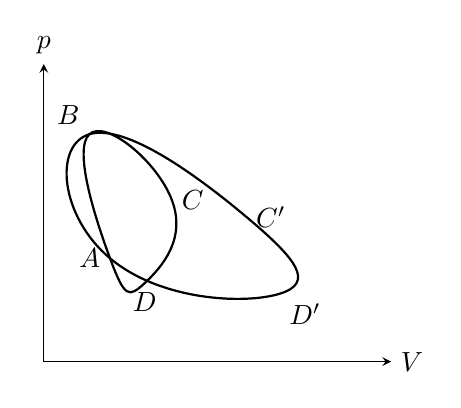
\begin{tikzpicture}[scale=1.05,>=stealth]
  \draw[->] (0,0) -- (4.2,0) node[right] {$V$};
  \draw[->] (0,0) -- (0,3.6) node[above] {$p$};
  \draw[thick,->] plot[smooth cycle,tension=0.95] coordinates {(0.8,1.25) (0.55,2.75) (1.55,1.95) (1.22,0.95)};
  \draw[thick,->] plot[smooth cycle,tension=0.95] coordinates {(0.8,1.25) (0.55,2.75) (2.45,1.75) (2.85,0.82)};
  \node[above left] at (0.55,2.75) {\(B\)};
  \node[left] at (0.8,1.25) {\(A\)};
  \node[right] at (1.55,1.95) {\(C\)};
  \node[below] at (1.22,0.95) {\(D\)};
  \node[right] at (2.45,1.75) {\(C'\)};
  \node[below right] at (2.85,0.82) {\(D'\)};
\end{tikzpicture}
\end{center}
\end{exercise}

\begin{solution}
\textbf{起手判断/模型：} 两个循环都夹在同一对高、低温热源之间，而且都是卡诺循环，所以效率只由两热源温度决定，不由循环在 \(p\)-\(V\) 图上画得多大决定。

\textbf{主方程：}
\[
\eta_{\text{Carnot}}=1-\frac{T_2}{T_1}.
\]
因此
\[
\eta_1=\eta_2.
\]

\textbf{净功比较：} 卡诺循环的净功等于 \(p\)-\(V\) 图围成的面积。图中第二个循环 \(ABC'D'A\) 的包围面积更大，所以它一循环输出的净功更大：
\[
W_1<W_2.
\]

\textbf{结论：}
\[
\boxed{\eta_1=\eta_2,\qquad W_1<W_2}
\]
对应选项 \(\boxed{\text{D}}\)。

\textbf{物理检查/易错点：} 不能拿“围成面积大小”去比较效率，因为效率只看热源温度；面积只比较净功。两个循环同样是卡诺循环，所以效率相等，但外圈循环吸收和释放的热都更多，净功也更多。
\end{solution}

\begin{exercise}[2010级期末：面积相等但温区不同的两个卡诺循环]
某理想气体分别进行两个 \(p\)-\(V\) 图上的卡诺循环 I 和 II。两循环曲线所围面积相等，即每循环输出净功相同。由图可判断循环 II 的高低温热源温差相对更大，故效率记为 \(\eta'\)；循环 I 的效率记为 \(\eta\)。若循环 I 每次从高温热源吸热 \(Q\)，循环 II 每次从高温热源吸热 \(Q'\)，比较 \(\eta,\eta'\) 以及 \(Q,Q'\)。
\end{exercise}

\begin{solution}
\textbf{起手判断/模型：} 卡诺效率只由两热源温度决定：
\[
\eta=1-\frac{T_2}{T_1}.
\]
按题图，循环 II 的温区使 \(T_2'/T_1'\) 更小，所以
\[
\eta<\eta'.
\]

\textbf{吸热比较：} 两循环围成面积相等，因此净功相等：
\[
A=A'.
\]
热机效率定义为
\[
\eta=\frac{A}{Q},\qquad \eta'=\frac{A'}{Q'}.
\]
在 \(A=A'\) 时，效率越小，完成同样输出功所需的高温吸热越多，因此
\[
Q>Q'.
\]

\textbf{结论：}
\[
\boxed{\eta<\eta',\qquad Q>Q'}.
\]

\textbf{物理检查/易错点：} 面积比较的是净功，不是效率。效率更高的热机用较少吸热就能输出同样的功，所以 \(Q\) 的大小与效率大小在本题中反向。
\end{solution}

\section{正循环与热机效率}

这一节要解决的问题是：热机效率到底在比较什么，它为什么总小于 \(1\)？

热机是持续地把热量转变为功的机器。对正循环，系统从高温热源吸热 \(Q_1\)，向低温热源放热 \(Q_2\)，并向外输出净功
\bridge{这一组记号最容易在正负号上出错，所以这里先约定：\(Q_1,Q_2\) 都按\textbf{与热源交换热量的大小}记正。若严格按“系统吸热为正、放热为负”的约定写，热机对应的是 \(+Q_1\) 和 \(-Q_2\)；制冷机对应的是 \(+Q_2\) 和 \(-Q_1\)。这样处理后，效率和致冷系数里的分子分母都直接表示“拿了多少”“放了多少”“搬了多少”的大小，而功的正负仍继续按系统对外做功的约定判。}
\[
A=Q_1-Q_2>0
\implies \eta=\frac{A}{Q_1}=\frac{Q_1-Q_2}{Q_1}=1-\frac{Q_2}{Q_1}.
\]

\begin{note}
\textbf{先看什么信号：} 题目若问“热机效率”或“吸收的热里有多少变成功”，分母一定先看高温热源吸收的 \(Q_1\)；\textbf{这条公式在控制什么：} 它控制的是输入热量中变成有用输出功的比例；\textbf{怎样最快记住：} 热机看的是“拿来多少高温热，最后留下多少功”；\textbf{最容易错：} 把效率错写成 \(A/Q_{\text{净}}\)，或者把制冷机的致冷系数公式和热机效率混用。
\end{note}

效率表示“从高温热源吸收的热量中，最后有多少比例变成了有用功”。只要还要向低温热源放热，就必然有 \(\eta<1\)。

\section{逆循环与致冷系数}

这一节要解决的问题是：为什么制冷机不用“效率”评价，而要改用“致冷系数”？

逆循环中，系统需要从外界获得输入功。按照本书符号，系统对外做功为 \(A<0\)，因此更方便单独记 \(A_{\text{in}}=-A>0\) 为\textbf{外界输入给系统的功的大小}。

制冷机从低温热源吸热 \(Q_2\)，向高温热源放热 \(Q_1\)，满足
\[
Q_1=A_{\text{in}}+Q_2
\implies \varepsilon=\frac{Q_2}{A_{\text{in}}}=\frac{Q_2}{Q_1-Q_2}.
\]

\begin{note}
\textbf{先看什么信号：} 题目若在问冰箱、空调、热泵或“输入多少功能搬走多少热”，就别写热机效率，先写致冷系数；\textbf{这条公式在控制什么：} 它控制的是搬运单位低温热量要付出多少外功；\textbf{怎样最快记住：} 热机看“拿热变功”，制冷机看“花功搬热”；\textbf{最容易错：} 继续沿用系统对外做功的符号 \(A\)，而不改用外界输入功的大小 \(A_{\text{in}}\)。
\end{note}

\begin{remark}
致冷系数衡量的是“为了搬运单位低温热量，需要付出多少外界功”。它可以大于 \(1\)，这并不违反能量守恒，因为它不是“输出功 / 输入能量”的效率，而是另一种评价指标。
\end{remark}

\section{卡诺循环、卡诺热机与卡诺制冷机}

这一节要解决的问题是：为什么课件把卡诺循环看得特别重，它到底提供了什么最核心的参考标准？

课件对卡诺循环的结构总结得很明确：
\begin{itemize}
  \item 工作物质只与两个恒温热源交换热量；
  \item 整个循环由两个\textbf{准静态等温过程}和两个\textbf{准静态绝热过程}组成。
\end{itemize}

对理想气体卡诺热机，常用过程顺序写成：
\begin{itemize}
  \item \(1\to2\)：在高温 \(T_1\) 下准静态等温膨胀并吸热；
  \item \(2\to3\)：准静态绝热膨胀，温度由 \(T_1\) 降到 \(T_2\)；
  \item \(3\to4\)：在低温 \(T_2\) 下准静态等温压缩并放热；
  \item \(4\to1\)：准静态绝热压缩，温度由 \(T_2\) 升回 \(T_1\)。
\end{itemize}

卡诺热机和卡诺制冷机的极限公式可并排记成
\[
\eta_{\text{Carnot}}=1-\frac{T_2}{T_1},\qquad
\varepsilon_{\text{Carnot}}=\frac{T_2}{T_1-T_2}.
\]

\begin{note}
\textbf{先看什么信号：} 题目一旦出现“同温区间卡诺极限”或“最高效率/最大致冷系数”，就直接切到卡诺公式；\textbf{这条公式在控制什么：} 它控制的是两个热源之间任何可逆装置所能达到的理论极限；\textbf{怎样最快记住：} 卡诺结论最关键的不是形式，而是“只看温度，不看工质”；\textbf{最容易错：} 用摄氏温度直接代入，或只记得热机那条，忘了制冷机的趋势恰好相反。
\end{note}

\begin{remark}
课件还专门提醒过：卡诺循环不一定总画成 \(p\)-\(V\) 图。若题目给的是 \(p\)-\(T\) 图、\(V\)-\(T\) 图或纯文字描述，第一步都必须先认清坐标轴，再判断哪两段是等温、哪两段是绝热。
\end{remark}

\begin{exercise}[2007级期末：一摩尔理想气体在两热源间作卡诺循环]
\(1\) mol 理想气体在 \(T_1=\SI{400}{K}\) 的高温热源与 \(T_2=\SI{300}{K}\) 的低温热源间作可逆卡诺循环。在 \(\SI{400}{K}\) 的等温线上，起始体积 \(V_1=\SI{0.001}{m^3}\)，终止体积 \(V_2=\SI{0.005}{m^3}\)。求每一循环中：1. 从高温热源吸收的热量 \(Q_1\)；2. 气体所作净功 \(W\)；3. 气体传给低温热源的热量 \(Q_2\)。
\end{exercise}

\begin{solution}
\textbf{起手判断/模型：} 卡诺循环由两段等温和两段绝热组成。高温等温膨胀段吸热，且理想气体等温过程 \(\Delta U=0\)，所以吸热等于等温膨胀功。

\textbf{求高温吸热：}
\[
Q_1=nRT_1\ln\frac{V_2}{V_1}.
\]
代入 \(n=1\)、\(R=\SI{8.31}{J/(mol.K)}\)，
\[
Q_1=1\times8.31\times400\ln5
\approx 5.35\times10^3\,\si{J}.
\]

\textbf{求净功：} 卡诺效率为
\[
\eta=1-\frac{T_2}{T_1}
=1-\frac{300}{400}
=0.25.
\]
所以
\[
W=\eta Q_1
\approx0.25\times5.35\times10^3
\approx1.34\times10^3\,\si{J}.
\]

\textbf{求低温放热：}
\[
Q_2=Q_1-W
\approx 5.35\times10^3-1.34\times10^3
\approx4.01\times10^3\,\si{J}.
\]

\textbf{结论：}
\[
\boxed{Q_1\approx5.35\times10^3\,\si{J}},\qquad
\boxed{W\approx1.34\times10^3\,\si{J}},\qquad
\boxed{Q_2\approx4.01\times10^3\,\si{J}}.
\]

\textbf{物理检查/易错点：} \(Q_2/Q_1=T_2/T_1=0.75\)，由上面的数值也约为 \(4.01/5.35\)，与可逆卡诺循环一致。
\end{solution}

\begin{exercise}[2005级期末：在最大效率下工作的热机每循环做功]
一热机从温度为 \(\SI{727}{\celsius}\) 的高温热源吸热，向温度为 \(\SI{527}{\celsius}\) 的低温热源放热。若热机在最大效率下工作，且每一循环吸热 \(\SI{2000}{J}\)，求此热机每一循环做功。
\end{exercise}

\begin{solution}
\textbf{起手判断/模型：} “最大效率”说明按卡诺热机极限处理。卡诺效率必须使用热力学温度，不能直接代摄氏温度。

\textbf{主方程：}
\[
\eta_{\max}=1-\frac{T_2}{T_1},\qquad
A=\eta Q_1.
\]

\textbf{分步代入或化简：} 温度换算为
\[
T_1=727+273=\SI{1000}{K},\qquad
T_2=527+273=\SI{800}{K}.
\]
所以
\[
\eta_{\max}=1-\frac{800}{1000}=0.20.
\]
每循环吸热 \(Q_1=\SI{2000}{J}\)，故
\[
A=\eta Q_1=0.20\times2000=\SI{400}{J}.
\]

\textbf{结论：}
\[
\boxed{A=\SI{400}{J}}.
\]

\textbf{物理检查/易错点：} 高低温差只有 \(200\,\si{K}\)，但高温热源在 \(1000\,\si{K}\) 量级，所以最大效率为 \(20\%\) 很合理。最容易错的是把 \(727\) 和 \(527\) 直接代入卡诺公式。
\end{solution}

\begin{exercise}[2010模拟题：空气卡诺热机的效率和每循环做功]
一卡诺热机以 \(\SI{290}{g}\) 空气为工作物质，工作在 \(\SI{27}{\celsius}\) 的高温热源和 \(\SI{-73}{\celsius}\) 的低温热源之间。若在高温等温膨胀过程中，气缸体积增大到原来的 \(2.718\) 倍，求该热机效率和每一循环所作的功。空气摩尔质量取 \(29\times10^{-3}\,\si{kg/mol}\)，\(R=\SI{8.31}{J/(mol.K)}\)。
\end{exercise}

\begin{solution}
\textbf{起手判断/模型：} 题目明确是卡诺热机，效率只由两热源的热力学温度决定；每循环做功则要先算高温等温膨胀吸热，再乘效率。

\textbf{温度和物质的量：}
\[
T_1=27+273=\SI{300}{K},\qquad
T_2=-73+273=\SI{200}{K}.
\]
\[
n=\frac{0.290}{29\times10^{-3}}=10\ \si{mol}.
\]

\textbf{效率：}
\[
\eta=1-\frac{T_2}{T_1}
=1-\frac{200}{300}
=\frac13.
\]

\textbf{高温等温吸热与循环功：} 高温等温膨胀时理想气体内能不变，吸热等于对外做功：
\[
Q_1=nRT_1\ln\frac{V_2}{V_1}.
\]
题中 \(V_2/V_1=2.718\approx e\)，故
\[
Q_1\approx 10\times 8.31\times300\times1
=\SI{2.493e4}{J}.
\]
卡诺热机每循环净功为
\[
A=\eta Q_1
\approx \frac13\times \SI{2.493e4}{J}
\approx \SI{8.31e3}{J}.
\]

\textbf{结论：}
\[
\boxed{\eta=\frac13},\qquad
\boxed{A\approx \SI{8.31e3}{J}}.
\]

\textbf{物理检查/易错点：} 温度必须换成 K；\(\SI{290}{g}\) 空气正好是 \(10\) mol。若把 \(27\) 和 \(-73\) 直接代入卡诺公式，会得到没有物理意义的效率。
\end{solution}

\begin{exercise}[电冰箱的输入功怎样由致冷系数反推]
一台电冰箱放在室温为 \(\SI{20}{\celsius}\) 的房间里，冰箱储藏柜温度维持在 \(\SI{5}{\celsius}\)。若每天有 \(2.0\times10^7\) J 的热量自房间传入冰箱内，且该冰箱的制冷系数是同温区间卡诺致冷机制冷系数的 \(55\%\)，求外界每天需对冰箱做多少功。
\end{exercise}

\begin{solution}
\textbf{起手判断/模型：} 题目研究的是\textbf{电冰箱}，所以第一步必须先把它认成逆循环装置，用的是致冷系数 \(\varepsilon\)，不是热机效率 \(\eta\)。而且涉及卡诺极限时，温度必须先换成热力学温度。

\textbf{主方程：} \(\varepsilon_{\text{Carnot}}=\frac{T_2}{T_1-T_2},\ \varepsilon=\frac{Q_2}{A_{\text{in}}}\)。

\textbf{分步代入或化简：} 先换温标：
\[
T_1=\SI{20}{\celsius}=293\ \si{K},\qquad
T_2=\SI{5}{\celsius}=278\ \si{K}
\implies \varepsilon_{\text{Carnot}}=\frac{278}{293-278}\approx 18.5.
\]
题目说实际冰箱只有卡诺值的 \(55\%\)，而维持柜内温度不变时，冰箱从低温区移走的热量大小就是每天漏入柜内的热量，因此
\[
\varepsilon=0.55\,\varepsilon_{\text{Carnot}}\approx 10.2,\qquad
Q_2=2.0\times10^7\ \si{J}
\implies
A_{\text{in}}=\frac{Q_2}{\varepsilon}
\approx \frac{2.0\times10^7}{10.2}
\approx 2.0\times10^6\ \si{J}.
\]

\textbf{结论：} 外界每天需对冰箱输入的功约为 \(A_{\text{in}}\approx 2.0\times10^6\ \si{J}\)。

\textbf{物理检查/易错点：} 输入功明显小于搬运的热量 \(Q_2\)，这对制冷机是正常的，因为它不是把功“全变成冷量”，而是在外功帮助下把热从低温区搬到高温区。最常见错误有两类：一是直接用摄氏温度代卡诺公式，二是把冰箱误当成热机去套效率定义。
\end{solution}

\begin{note}
课件最后还给了奥托机作为应用例题。它不是本章主线，但很适合做方法回顾：若一个循环由两段等体过程和两段绝热过程组成，就继续按“逐段列出 \(Q\)、\(A\)、\(\Delta U\)，最后再求总效率”的统一方法处理。
\end{note}

\begin{exercise}[1 mol 氦气矩形循环怎样逐段写出吸放热]
1 mol 氦气经历如图所示的矩形循环，其中 \(p_2=2p_1,\ V_4=2V_1\)。求各过程 \(1\to2,\ 2\to3,\ 3\to4,\ 4\to1\) 中气体吸收的热量，并求该热机效率。
\end{exercise}

\begin{solution}
\textbf{起手判断/模型：} 这是一个循环题，但题目不是只问总效率，而是先问四段各自的吸放热，所以第一步不能只写 \(\Delta U=0\)，而应先认出每一段各是什么过程，再逐段写 \(Q\)。

\textbf{主方程：}
\[
T=\frac{pV}{R},\qquad
Q_{\text{等体}}=C_{V,m}\Delta T,\qquad
Q_{\text{等压}}=C_{P,m}\Delta T,\qquad
\eta=\frac{A}{Q_1}.
\]

\textbf{分步代入或化简：} 由状态方程，
\[
T_2=\frac{p_2V_1}{R}=2T_1,\qquad
T_3=\frac{p_2V_4}{R}=4T_1,\qquad
T_4=\frac{p_1V_4}{R}=2T_1.
\]
于是四段吸热量可压成
\[
\begin{aligned}
Q_{12}&=C_{V,m}(T_2-T_1)=C_{V,m}T_1,\\
Q_{23}&=C_{P,m}(T_3-T_2)=2C_{P,m}T_1,\\
Q_{34}&=C_{V,m}(T_4-T_3)=-2C_{V,m}T_1,\\
Q_{41}&=C_{P,m}(T_1-T_4)=-C_{P,m}T_1.
\end{aligned}
\]
对单原子理想气体氦，
\[
C_{V,m}=\frac{3}{2}R,\qquad C_{P,m}=\frac{5}{2}R,
\]
故
\[
\begin{aligned}
Q_{12}&=\frac{3}{2}RT_1,\\
Q_{23}&=5RT_1,\\
Q_{34}&=-3RT_1,\\
Q_{41}&=-\frac{5}{2}RT_1.
\end{aligned}
\]
总吸热只取正的两段：
\[
Q_1=Q_{12}+Q_{23}=\frac{13}{2}RT_1.
\]
循环净功等于矩形面积：
\[
A=(p_2-p_1)(V_4-V_1)=p_1V_1=RT_1.
\]
因此
\[
\eta=\frac{A}{Q_1}=\frac{RT_1}{\frac{13}{2}RT_1}=\frac{2}{13}\approx 15.4\%.
\]

\textbf{结论：}
\[
Q_{12}=\frac{3}{2}RT_1,\quad
Q_{23}=5RT_1,\quad
Q_{34}=-3RT_1,\quad
Q_{41}=-\frac{5}{2}RT_1,\quad
\eta\approx 15.4\%.
\]

\textbf{物理检查/易错点：} 四段里两段吸热、两段放热，这和 \(p\)-\(V\) 图上“先升温后降温”的图景一致。最容易错的是把等压段的热量还写成 \(C_V\Delta T\)，或者把效率分母误写成净热量。
\end{solution}

\begin{exercise}[两条 \(p\)-\(V\) 过程线怎样只靠第一定律判断吸热还是放热]
一定量理想气体分别经历两条过程线 \(abc\) 与 \(def\)。其中 \(abc\) 为等温膨胀后再继续膨胀的一类过程，\(def\) 为压缩过程。怎样只靠 \(Q=\Delta U+A\) 判断它们分别是吸热还是放热？
\end{exercise}

\begin{solution}
\textbf{起手判断/模型：} 这题的关键不是算数字，而是先判三件事的符号：\(\Delta U\) 正负如何、系统对外做功 \(A\) 正负如何、于是 \(Q\) 的总符号怎样。也就是说，第一条方程就该写第一定律，而不是急着找具体状态量数值。

\textbf{主方程：}
\[
Q=\Delta U+A.
\]

\textbf{分步代入或化简：} 对过程 \(abc\)，气体总体在膨胀，故
\[
A>0.
\]
其中若含等温段，则该段有 \(\Delta U=0\)；而若整体末态温度不低于初态，则总的 \(\Delta U\ge 0\)。因此
\[
Q=\Delta U+A>0,
\]
故 \(abc\) 为吸热过程。

对过程 \(def\)，若末态温度降低，则
\[
\Delta U<0.
\]
同时过程为压缩，系统对外做功为负，即
\[
A<0.
\]
于是
\[
Q=\Delta U+A<0,
\]
故 \(def\) 为放热过程。

\textbf{结论：} 过程 \(abc\) 吸热，过程 \(def\) 放热。

\textbf{物理检查/易错点：} 这类题真正考的是“先判符号，再谈数值”。只要 \(\Delta U\) 和 \(A\) 的符号都判清，很多图像题根本不必算出每一个状态量。
\end{solution}

\begin{exercise}[氧气作 \(ABCD\) 循环时效率为什么先看哪两段吸热]
质量为 \(32\times10^{-3}\,\si{kg}\) 的氧气作 \(ABCD\) 循环，其中 \(A\to B\) 与 \(C\to D\) 为等温过程，\(T_1=\SI{300}{K}\)、\(T_2=\SI{200}{K}\)、\(V_2=2V_1\)。求该循环效率。
\end{exercise}

\begin{solution}
\textbf{起手判断/模型：} 题目问效率，最重要的不是先求总功，而是先判\textbf{哪些过程在吸热}，因为效率分母是总吸热 \(Q_1\)。这一步若先搞反，后面全部会错。

\textbf{主方程：}
\[
\eta=\frac{A}{Q_1},\qquad
Q_{\text{等温}}=nRT\ln\frac{V_2}{V_1},\qquad
Q_{\text{定容}}=nC_{V,m}\Delta T.
\]

\textbf{分步代入或化简：} 由题给氧气质量正好是 1 mol，所以 \(n=1\)。逐段看：
\[
\begin{aligned}
Q_{AB}&=RT_1\ln\frac{V_2}{V_1}>0,\\
Q_{BC}&=C_{V,m}(T_2-T_1)<0,\\
Q_{CD}&=RT_2\ln\frac{V_1}{V_2}<0,\\
Q_{DA}&=C_{V,m}(T_1-T_2)>0.
\end{aligned}
\]
氧气近似看作双原子理想气体，
\[
C_{V,m}=\frac{5}{2}R.
\]
因此总吸热为
\[
Q_1=Q_{AB}+Q_{DA}
=RT_1\ln\frac{V_2}{V_1}+\frac{5}{2}R(T_1-T_2).
\]
循环净功只来自两段等温过程之和：
\[
\begin{aligned}
A&=Q_{AB}+Q_{CD}\\
&=RT_1\ln\frac{V_2}{V_1}+RT_2\ln\frac{V_1}{V_2}\\
&=R(T_1-T_2)\ln\frac{V_2}{V_1}.
\end{aligned}
\]
代入 \(T_1=300\,\si{K},\ T_2=200\,\si{K},\ V_2/V_1=2\) 得
\[
\eta=\frac{100R\ln 2}{300R\ln 2+250R}\approx 15\%.
\]

\textbf{结论：} 循环效率约为 \(15\%\)。

\textbf{物理检查/易错点：} 本题最容易错在把两段等温都当成吸热。其实高温等温膨胀吸热，低温等温压缩放热；只有先把热流方向判清，效率分母才不会错。
\end{solution}

\begin{exercise}[水蒸气 \(abcda\) 循环怎样逐段做能量账]
气缸内有 \(\SI{36}{g}\) 水蒸气，视为刚性分子理想气体，经历如图所示 \(abcda\) 循环。其中 \(a\to b\)、\(c\to d\) 为等体过程，\(b\to c\) 为等温过程，\(d\to a\) 为等压过程。已知 \(p_a=p_d=2\,\mathrm{atm}\)、\(p_b=6\,\mathrm{atm}\)、\(V_a=V_b=\SI{25}{L}\)、\(V_c=V_d=\SI{50}{L}\)。求：1. \(d\to a\) 过程水蒸气做功；2. \(a\to b\) 内能增量；3. 循环净功；4. 循环效率。

\begin{center}

\includegraphics[width=0.34\linewidth]{pdf-exercises/pdf2003-q22-pv-cycle.png}
\end{center}
\end{exercise}

\begin{solution}
\textbf{起手判断/模型：} 循环题不要一眼看图就套单一公式，而要逐段认过程。这里 \(a\to b\) 等体，\(b\to c\) 等温，\(c\to d\) 等体，\(d\to a\) 等压；循环一周后 \(\Delta U_{\text{cycle}}=0\)，净功就是图中围成的面积对应的代数和。

\textbf{已知量换算：} 水蒸气摩尔质量 \(M_{\mathrm{mol}}=\SI{18e-3}{kg/mol}\)，所以
\[
n=\frac{36\times10^{-3}}{18\times10^{-3}}=\SI{2}{mol}.
\]
刚性水分子常取自由度 \(i=6\)，故
\[
U=\frac{i}{2}nRT=3nRT,\qquad \Delta U=\frac{i}{2}\Delta(pV)=3\Delta(pV).
\]

\textbf{分步计算：} \(d\to a\) 为等压压缩，
\[
W_{da}=p_a(V_a-V_d)
=2\times1.013\times10^5\times(25-50)\times10^{-3}
\approx -\SI{5.07e3}{J}.
\]
\(a\to b\) 为等体过程，
\[
\Delta U_{ab}=3V_a(p_b-p_a)
=3\times25\times10^{-3}\times(6-2)\times1.013\times10^5
\approx \SI{3.04e4}{J}.
\]
\(b\to c\) 为等温膨胀，且 \(p_bV_b=6\times25=p_cV_c\)，所以
\[
W_{bc}=nRT_b\ln\frac{V_c}{V_b}
=p_bV_b\ln2
=6\times1.013\times10^5\times25\times10^{-3}\ln2
\approx \SI{1.05e4}{J}.
\]
循环净功为
\[
W=W_{bc}+W_{da}\approx \SI{5.47e3}{J}.
\]
吸热发生在 \(a\to b\) 与 \(b\to c\)，其中 \(Q_{ab}=\Delta U_{ab}\)，\(Q_{bc}=W_{bc}\)，故
\[
Q_1=Q_{ab}+Q_{bc}
\approx \SI{4.09e4}{J}.
\]
循环效率
\[
\eta=\frac{W}{Q_1}
\approx \frac{5.47\times10^3}{4.09\times10^4}
\approx 0.13.
\]

\textbf{结论：}
\[
\boxed{W_{da}\approx-\SI{5.07e3}{J},\quad
\Delta U_{ab}\approx\SI{3.04e4}{J},\quad
W\approx\SI{5.47e3}{J},\quad
\eta\approx 13\%.}
\]

\textbf{物理检查/易错点：} \(d\to a\) 是压缩，系统对外做功为负；\(b\to c\) 是等温膨胀，功为正。效率必须用循环净功除以总吸热，不能用净功除以某一段热量。
\end{solution}

\begin{exercise}[同压从状态 \(A\) 到状态 \(B\) 时哪个量必然改变]
一定量理想气体由平衡态 \(A\) 变到平衡态 \(B\)，且 \(p_A=p_B\)，图中 \(B\) 的体积大于 \(A\)。无论经历什么过程，判断系统哪一项一定成立：对外作正功、内能增加、从外界吸热、向外界放热。

\begin{center}

\includegraphics[width=0.24\linewidth]{pdf-exercises/pdf2004-q06-pv-ab.png}
\end{center}
\end{exercise}

\begin{solution}
\textbf{起手判断/模型：} 题目强调“无论经过什么过程”，说明只能用状态量判断，不能用依赖路径的功和热量判断。理想气体内能只与温度有关，而温度由状态方程决定。

\textbf{状态方程：}
\[
pV=nRT.
\]
由于 \(p_A=p_B\) 且 \(V_B>V_A\)，所以
\[
T_B>T_A.
\]
理想气体内能满足
\[
U=\frac{i}{2}nRT,
\]
故
\[
\Delta U>0.
\]

\textbf{结论：}
\[
\boxed{\text{系统内能必然增加}.}
\]

\textbf{物理检查/易错点：} 功和热量都是过程量，同一初末态可以走不同路径，所以不能说“必然对外作正功”或“必然吸热”。只有温度和内能这类状态量能由初末态直接判断。
\end{solution}

\begin{exercise}[标准状态理想气体两条路径到同一终态的吸热]
一定量理想气体在标准状态下体积为 \(V_1=1.0\times10^{-2}\,\si{m^3}\)。求下列过程中气体吸收的热量：1. 等温膨胀到 \(V_2=2.0\times10^{-2}\,\si{m^3}\)；2. 先等体冷却，再等压膨胀到第 1 问的终态。已知 \(1\,\mathrm{atm}=1.013\times10^5\,\si{Pa}\)，并设气体 \(C_V=5R/2\)。
\end{exercise}

\begin{solution}
\textbf{起手判断/模型：} 两个过程初末态相同，但路径不同，所以吸热量不一定相同。第一问等温，理想气体 \(\Delta U=0\)；第二问先等体再等压，仍因初末温度相同而总 \(\Delta U=0\)，但功不同。

\textbf{1. 等温膨胀：}
\[
Q_1=W_1=\int_{V_1}^{V_2}\frac{p_1V_1}{V}\,\dd V
=p_1V_1\ln\frac{V_2}{V_1}.
\]
代入
\[
Q_1=1.013\times10^5\times1.0\times10^{-2}\ln2
\approx \SI{7.02e2}{J}.
\]

\textbf{2. 等体冷却再等压膨胀：} 终态与初态温度相同，且 \(V_2=2V_1\)，故终态压强
\[
p_2=\frac{p_1V_1}{V_2}=\frac12p_1.
\]
全过程 \(\Delta U=0\)，等体段不做功，只有等压膨胀段做功：
\[
Q_2=W_2=p_2(V_2-V_1)
=\frac12p_1(V_2-V_1).
\]
代入
\[
Q_2=\frac12\times1.013\times10^5\times(2.0-1.0)\times10^{-2}
\approx \SI{5.07e2}{J}.
\]

\textbf{结论：}
\[
\boxed{Q_1\approx\SI{7.02e2}{J}},\qquad
\boxed{Q_2\approx\SI{5.07e2}{J}}.
\]

\textbf{物理检查/易错点：} 两条路径初末温度相同，所以总内能变化相同且为零；但功是路径量，等温曲线下的面积比“低压等压线”下的面积大，因此第一问吸热更多。
\end{solution}

\begin{exercise}[奥托循环效率为什么自然写成压缩比的函数]
奥托机循环由两段等体过程和两段绝热过程组成，其中 \(c\to d\)、\(e\to b\) 为等体过程，\(b\to c\)、\(d\to e\) 为绝热过程。设压缩比为 \(r=V/V_0\)。求循环效率。
\end{exercise}

\begin{solution}
\textbf{起手判断/模型：} 奥托循环的热交换只发生在两段等体过程中，所以第一条方程不该先写总功，而应先写吸热段和放热段的 \(Q\)。随后再用绝热关系把温度比改写成体积比。

\textbf{主方程：}
\[
\eta=1-\frac{Q_2}{Q_1},\qquad
Q_1=C_{V,m}(T_d-T_c),\qquad
Q_2=C_{V,m}(T_e-T_b).
\]

\textbf{分步代入或化简：} 先写效率：
\[
\eta=1-\frac{T_e-T_b}{T_d-T_c}.
\]
两段绝热过程分别满足
\[
T_eV^{\gamma-1}=T_dV_0^{\gamma-1},\qquad
T_bV^{\gamma-1}=T_cV_0^{\gamma-1}.
\]
两式相减可得
\[
(T_e-T_b)V^{\gamma-1}=(T_d-T_c)V_0^{\gamma-1}
\implies
\frac{T_e-T_b}{T_d-T_c}=\left(\frac{V_0}{V}\right)^{\gamma-1}.
\]
于是
\[
\eta=1-\left(\frac{V_0}{V}\right)^{\gamma-1}
=1-\frac{1}{r^{\gamma-1}}.
\]

\textbf{结论：}
\[
\boxed{\eta=1-\frac{1}{r^{\gamma-1}}},\qquad r=\frac{V}{V_0}.
\]

\textbf{物理检查/易错点：} 压缩比 \(r\) 越大，效率越高，这和“压缩得越狠，绝热升温越明显，循环更容易把热转成净功”的图景一致。最容易错的是把吸热段、放热段写反，或把绝热关系里的体积比倒过来。
\end{solution}

\section{常见误区}

\begin{itemize}
  \item 把 \(Q\)、\(A\) 和 \(U\) 都当成状态量，或者把 \(\delta Q\) 误写成 \(dQ\)。
  \item 看到“过程很慢”就机械当成准静态，却不先检查是否始终近似平衡。
  \item 看见“绝热”就立刻套 \(pV^\gamma=\text{const}\)，忽略了它只适用于准静态绝热过程。
  \item 在逆循环题里仍把系统对外做功的符号 \(A\) 直接拿去算致冷系数，而不改用输入功的大小 \(A_{\text{in}}\)。
  \item 忘记循环过程里 \(\Delta U=0\)，从而把状态量和过程量混着算。
\end{itemize}

\section{章末小结}

\summaryline{热力学第一定律的主线是：先用准静态和平衡态保证过程可描述，再用 \(Q=\Delta U+A\) 统计能量收支，然后把理想气体的等体、等压、等温、绝热、多方和循环过程全部纳入同一套“先判过程类型，再跟踪 \(Q\)、\(A\) 和 \(\Delta U\)”的框架。}
\chapterselfcheck{为什么只有当宏观变化时间远大于弛豫时间时，准静态近似才可靠？为什么 \(\delta Q=dU+p\,\dd V\) 里只有 \(U\) 是状态量？为什么绝热线比等温线更陡？为什么绝热自由膨胀不能套绝热方程？为什么逆循环必须改用输入功大小来定义致冷系数？}

\chapter{热力学第二定律}

\begin{skill}[第12章冲刺总手册]\label{sk:phys-ch12-overview}
\textbf{【这章先解决什么题】} 这章处理“能量够不够之外，这个过程能不能自发发生”的题：可逆与不可逆、卡诺极限、熵变计算、总熵增和热过程方向判断。

\textbf{【拿题先认什么信号】} 若题面问“能不能自发发生、最大效率是多少、总熵怎样变、可逆还是不可逆”，就进入第二定律；若题面只是算 \(Q\)、\(A\)、\(\Delta U\)，那还是第一定律入口。

\textbf{【第一条方程先写什么】}
\[
dS=\frac{\delta Q_{\mathrm{rev}}}{T}.
\]
它不是说过程必须真的可逆，而是说\textbf{熵是状态量}，所以很多不可逆过程也可以沿一条假想可逆路径来算同样的 \(\Delta S\)。

\textbf{【必背公式块】}
\[
\begin{aligned}
\Delta S&=\int \frac{\delta Q_{\mathrm{rev}}}{T},\\
\text{理想气体：}\quad
\Delta S&=nC_{V,m}\ln\frac{T_2}{T_1}+nR\ln\frac{V_2}{V_1}\\
&=nC_{P,m}\ln\frac{T_2}{T_1}-nR\ln\frac{p_2}{p_1},\\
\text{可逆绝热：}\quad
\Delta S&=0,\\
\text{孤立系统：}\quad
\Delta S_{\text{总}}&\ge 0,\\
\text{卡诺热机：}\quad
\eta_{\text{Carnot}}&=1-\frac{T_2}{T_1}.
\end{aligned}
\]
其中 \(T_1\) 取高温热源温度，\(T_2\) 取低温热源温度，必须用绝对温标 \(\si{K}\)。

\textbf{【做题流程】} 先问题目是在算数值熵变，还是在判方向/极限；若算熵变，就先选一条最容易积分的可逆辅助路径；若判自发性，就看孤立系统或系统加环境的总熵变；若求效率极限，就直接切到卡诺结论，而不是在具体装置细节里兜圈。

\textbf{【最容易误判】} 把“绝热”直接等同于“熵不变”，其实只有可逆绝热才有 \(\Delta S=0\)；只算系统熵变，不算环境熵变就妄下自发结论；卡诺效率里把摄氏温度直接代入。

\textbf{【最后怎样验证】} 不可逆孤立过程应满足 \(\Delta S_{\text{总}}>0\)；可逆过程才可能取等号；热机效率不可能超过卡诺效率；若沿辅助可逆路径算出的熵变和初末态不符，通常是路径积分或温标写错。
\end{skill}

\chapterroadmap
{回答“为什么过程有方向”，并把这种方向性定量化。}
{已经会用第一定律处理能量收支，也知道一些常见热过程。}
{新增可逆/不可逆、开尔文/克劳修斯表述、熵、熵变和熵增加原理。}

\bridge{第二定律不是替第一定律改账本，而是告诉你：即便能量守恒，过程也不一定能自发发生。熵就是把这种“方向性”写成数学量。}

\section{为什么还需要第二定律}

这一节要解决的问题是：既然第一定律已经告诉我们“能量守恒”，为什么热学里还要再引入第二定律。

第一定律只告诉我们能量守恒，却没有告诉我们过程能否自发发生。例如热量从高温物体传到低温物体是自发的，但反向过程不会自发发生。要描述这种方向性，就需要第二定律。

\bridge{换句话说，第一定律只负责排除“账算错了”的过程，却排除不了“账没错但方向不对”的过程。第二定律补上的，正是这种自发方向与可逆性的限制。}

可以把两条定律分工得很清楚：
\begin{itemize}
  \item 第一定律回答“账对不对”，也就是吸了多少热、做了多少功、内能怎么变；
  \item 第二定律回答“方向对不对”，也就是这个过程会不会自己发生、能不能不留代价地完全倒回来。
\end{itemize}

\begin{remark}
如果只靠第一定律，你很难排除一些“账面上不矛盾，但现实里从不自己发生”的过程。第二定律就是专门把这些“方向性限制”补进来。
\end{remark}

\section{第二定律的两种经典表述}

\begin{theorem}[开尔文表述]\label{thm:kelvin-statement}
不可能从单一热源吸热，并把吸收的热量全部转化为有用功而不产生其他影响。
\end{theorem}

\begin{theorem}[克劳修斯表述]\label{thm:clausius-statement}
热量不可能自发地从低温物体传到高温物体而不引起其他变化。
\end{theorem}

这两种表述看起来一个在讲热机，一个在讲传热，其实说的是同一件事：\textbf{热现象存在天然方向，不能任意无代价地反过来。}

\begin{itemize}
  \item 开尔文表述强调：热不可能百分之百、无附带代价地全部变成功。
  \item 克劳修斯表述强调：热不可能自己从冷的地方跑到热的地方。
\end{itemize}

\begin{note}
\textbf{先看什么信号：} 题目若在问“热能能不能全部变功”或“热能能不能自己从冷到热”，就是第二定律入口；\textbf{这条公式在控制什么：} 两种表述控制的都是热过程的天然方向，分别落在热机和传热两个场景；\textbf{怎样最快记住：} 开尔文抓“单一热源不能全变功”，克劳修斯抓“热不会自发冷到热”，两句都在说不可逆方向；\textbf{最容易错：} 把它们记成互不相干的两条禁令，而没看出它们其实是同一方向性原则的两种说法。
\end{note}

\section{热力学第二定律的应用：卡诺定理}

这一节要解决的问题是：在同样的高温热源和低温热源之间工作时，热机效率到底有没有上限。

如果不先把“为什么会有上限”讲清，卡诺定理很容易被读成另一条结论表。更自然的入口是反证法：\textbf{假如真有一台热机效率比同温度区间上的可逆热机还高，那么把这台“更高效热机”和一台反向运行的可逆机拼在一起，就能制造出违背第二定律的装置。} 比如可以让高效热机带着可逆机倒着跑，结果系统可能变成“只从单一热源吸热就全部变成功”，或者“没有外功输入却把热从冷源搬到热源”，这分别直接撞上开尔文表述或克劳修斯表述。也就是说，卡诺效率上限不是经验总结，而是第二定律逼出来的极限。

\begin{theorem}[卡诺定理]
在相同高温热源 \(T_1\) 和低温热源 \(T_2\) 之间工作的任意可逆热机都具有相同的效率；在这两个热源之间工作的任意不可逆热机的效率都不可能大于可逆热机的效率。
\end{theorem}

热机中，系统从高温热源吸热 \(Q_1>0\)，向低温热源放热 \(Q_2<0\)，于是
\[
A=Q_1+Q_2=Q_1-|Q_2|
\implies
\eta=\frac{A}{Q_1}=\frac{Q_1-|Q_2|}{Q_1}.
\]

\bridge{这里写成 \(|Q_2|\) 不是为了凑符号，而是为了提醒读者：放热本身是“流出”的能量，和吸热的正号约定不同，所以公式里必须先把大小和方向拆开。}

\begin{note}
\textbf{先看什么信号：} 题目若把放热写成负值，效率式里就要先把大小和方向拆开；\textbf{这条公式在控制什么：} 它控制的是在统一符号约定下，怎样把“吸热减放热”翻成输出功；\textbf{怎样最快记住：} 高温热源给进来的叫 \(Q_1\)，低温热源带走的那部分先取大小 \(|Q_2|\)，再谈效率；\textbf{最容易错：} 一边把 \(Q_2\) 当负数，一边又在公式里再减一次，导致符号重复处理。
\end{note}

\begin{remark}
开尔文表述和克劳修斯表述是同一条第二定律的两种说法；如果其中一个不成立，另一个也会随之不成立。这就是课件里强调的“不可逆性的相互依存”。
\end{remark}

\section{可逆过程与不可逆过程}

这一节第一次读最该先问的是：为什么讨论熵前，非得绕到“可逆”这个听起来很理想化的概念上？因为第一定律只管能量守恒，不管过程方向；可我们现在要找的是一种既能区分“自然会往哪边走”，又能长成状态量的新记账法。而若中间充满摩擦、有限温差传热和剧烈不平衡，热量元与系统温度就没法一一配对，\(\delta Q/T\) 也就无法稳定地长成状态量。所以必须先抓住可逆极限，才能把熵定义干净。

\begin{definition}[可逆过程]\label{def:reversible-process}
若系统和外界都能沿原路径严格返回初态，并且不留下任何额外影响，则该过程称为\textbf{可逆过程}。
\end{definition}

现实中的大多数过程都是不可逆过程，例如有摩擦的机械过程、有限温差传热、自由膨胀等。

判断可逆与不可逆时，最容易混淆的是“能不能想办法倒回去”和“是不是可逆过程”。这两者不是一回事。许多过程当然可以靠外力强行反着做回去，但如果这样做时系统或外界留下了别的变化，那么它仍然不是可逆过程。

\begin{note}
“能反着做回来”并不等于“可逆”。可逆要求系统和外界都恢复原状，且不留下任何额外影响，这是很强的条件，所以现实过程大多只是“接近可逆”，很少真正可逆。
\end{note}

\begin{remark}
非准静态过程通常不可逆，因为系统来不及在每一瞬间都保持近似平衡。摩擦、有限温差传热和自由膨胀，都是最典型的不可逆来源。
\end{remark}

\begin{remark}
一个很有用的判断标准是：这个过程是否足够缓慢、是否几乎没有摩擦和耗散、是否没有有限温差下的直接传热。只要这些理想条件破掉了，可逆性通常也就破掉了。
\end{remark}

\section{熵的初步概念}

\textbf{本节问题：} 第一定律已经能管”能量账”，为什么热学还要再引入一个新量，而且这个新量还能帮助我们判断过程方向？

\bridge{这一步最好分三层读，而不要一口气压过去。第一层，只看一台可逆卡诺机：它在两条等温线上交换热量 \(Q_1,Q_2\)，又因为效率只取决于 \(T_1,T_2\)，于是
\[
\eta=1-\frac{T_2}{T_1}
=\frac{Q_1-|Q_2|}{Q_1}
\implies
\frac{Q_1}{T_1}=\frac{|Q_2|}{T_2}.
\]
第二层，把任意可逆循环想成很多个无穷小卡诺循环拼起来，于是整圈都会满足
\[
\oint \frac{\delta Q_{\mathrm{rev}}}{T}=0.
\]
第三层，既然这类环路积分总为零，它就应当来自某个状态函数的全微分，这个被逼出来的状态函数才叫熵。这样走下来，\(dS=\delta Q_{\mathrm{rev}}/T\) 就不再像“聪明定义”，而是卡诺图景一路推到头的自然结果。}

\begin{remark}
"环路积分为零 \(\Rightarrow\) 全微分"这一步的数学含义：如果一个量 \(\delta Q_{\mathrm{rev}}/T\) 沿任意闭合路径积分都为零，那么它从状态 A 到状态 B 的积分就与路径无关（因为任何两条路径构成一个闭合回路）。路径无关意味着积分值只取决于端点，因此存在一个状态函数 \(S\) 使得 \(\dd S=\delta Q_{\mathrm{rev}}/T\)。这和微积分中"保守力做功与路径无关 \(\Rightarrow\) 存在势能函数"是完全相同的数学结构。
\end{remark}

\bridge{为什么要除以 \(T\)？直觉上：同样传递 \(\SI{1}{J}\) 的热量，给 \(\SI{300}{K}\) 的物体和给 \(\SI{3}{K}\) 的物体，后者的”混乱程度”增加得远比前者多。除以 \(T\) 正是在衡量”这份热量对微观状态数的影响有多大”。温度越低，同样的热量能打开的新微观状态越多，所以贡献的熵变越大。}

\textbf{物理图景：} 热过程里最难处理的不是能量够不够，而是过程会不会自发往某个方向走。热从高温流向低温、气体自由膨胀、两种物质自行混合，这些过程在账面上都不违背能量守恒，但它们明显带有方向性。熵就是专门用来把这种方向性写成可计算量的。

\textbf{核心判据/公式：} 在可逆过程中，
\[
\Delta S=\int \frac{\delta Q_{\mathrm{rev}}}{T},\qquad
\oint \frac{\delta Q_{\mathrm{rev}}}{T}=0.
\]
前者给出熵变定义，后者就是课件反复使用的克劳修斯等式。它说明热温比沿可逆循环积分为零，于是这个积分只由初末状态决定，熵因此可以被当作\textbf{状态量}。

\textbf{公式为何这样写：} 式子里最关键的不是积分号，而是下标 \(\mathrm{rev}\)。只有在可逆过程中，系统经历的每个中间状态都足够接近平衡，热量元 \(\delta Q_{\mathrm{rev}}\) 才能和当时的温度 \(T\) 一一对应；也只有这样，\(\delta Q_{\mathrm{rev}}/T\) 才能成为定义状态量的合格“微元”。

\textbf{常见误判或适用边界：} 熵不是“无序程度”这四个字就能替代完的口号，更不能把任意过程里的 \(\delta Q/T\) 直接拿来积分。真实过程若不可逆，仍然要借助一条连接同样初末状态的\textbf{假想可逆路径}来算 \(\Delta S\)。所以这一节最稳的理解顺序是：先认清方向性需要新量，再认清这个新量为何用可逆过程定义，最后再认清状态量允许我们把不可逆问题改成可逆积分问题。

\begin{note}
\textbf{先看什么信号：} 题目若在问“过程方向”“能否自发发生”或“同一初末态下不可逆过程怎样算熵变”，就要切到熵；\textbf{这条公式在控制什么：} 它控制的是热量交换在给定温度下对状态量的贡献；\textbf{怎样最快记住：} 熵变不是直接记“吸了多少热”，而是记“在什么温度下吸了多少可逆热”；\textbf{最容易错：} 把任意真实过程的 \(\delta Q/T\) 直接积分，而不先改成一条可逆计算路径。
\end{note}

\section{熵的计算}

这里最值得先压成口令的一句话是：\textbf{熵是状态量，所以先固定起点和终点，再专门挑一条最容易积分的可逆辅助路径。} 也就是说，真实过程本身哪怕不可逆，我们也不必沿那条难算的真实路去算熵变；我们真正算的是“连接同样初末态时，可逆热温比积分会给出多少”。

对理想气体，先把桥接链拆开看最稳：由熵的定义，\(\delta Q_{\mathrm{rev}}=TdS\)；由可逆准静态体积功下的第一定律，\(\delta Q_{\mathrm{rev}}=dU+p\,\dd V\)。把这两条并在一起，才得到后面真正好用的桥接关系：
\[
TdS=\delta Q_{\mathrm{rev}}=dU+p\,\dd V.
\]
这说明熵的计算，本质上还是要回到“先找一条方便积分的可逆路径”。

如果想知道后面的对数到底从哪来，最稳的办法就是把理想气体的两本账代回这条桥接式：一方面
\[
dU=nC_{V,m}\,dT,
\]
另一方面
\[
p=\frac{nRT}{V}.
\]
于是
\[
TdS=nC_{V,m}\,dT+\frac{nRT}{V}\,dV
\implies
dS=nC_{V,m}\frac{dT}{T}+nR\frac{dV}{V}.
\]
这已经把“为什么会出现对数”说透了，因为后面只是对 \(dT/T\) 和 \(dV/V\) 做积分。若换用状态方程消去 \(dV\)，同样也可压成
\[
dS=nC_{P,m}\frac{dT}{T}-nR\frac{dp}{p}.
\]
所以 \(C_V\) 版和 \(C_P\) 版并不是两套互不相干的经验公式，而只是同一条熵微分式在不同变量选择下的两种展开。

\begin{note}
\textbf{先看什么信号：} 题目一旦不给现成熵变公式，或者过程本身看起来不好直接积分，就先回到这条桥接式；\textbf{这条公式在控制什么：} 它把熵、热量、内能和体积功连到一起，是后面各种 \(\Delta S\) 对数公式的共同起点；\textbf{怎样最快记住：} 先记“熵变要靠可逆热温比定义”，再记“理想气体里 \(\delta Q_{\mathrm{rev}}\) 还能拆成 \(dU+p\,dV\)”；\textbf{最容易错：} 直接把后面某个现成公式硬套到陌生过程上，而不先判断能不能选一条更方便的可逆路径。
\end{note}

下面这组对数公式都默认了同一前提：\textbf{对象是理想气体，而且我们已经改选成一条方便积分的可逆参考路径。} 其中“准静态绝热过程熵变为零”也只在可逆绝热条件下成立。带着这层前提，再看几类常见过程的熵变公式：
\begin{align*}
\text{等体过程:}\quad \Delta S&=nC_{V,m}\ln\frac{T_2}{T_1},\\
\text{等压过程:}\quad \Delta S&=nC_{P,m}\ln\frac{T_2}{T_1},\\
\text{等温过程:}\quad \Delta S&=nR\ln\frac{V_2}{V_1}=nR\ln\frac{p_1}{p_2},\\
\text{准静态绝热过程:}\quad \Delta S&=0.
\end{align*}

\begin{note}
\textbf{先看什么信号：} 熵变题先看初末态和过程类型，再决定该用 \(C_V\)、\(C_P\) 还是 \(nR\)；\textbf{这条公式在控制什么：} 它们控制的是不同可逆路径下，热温比积分怎样落成对数形式；\textbf{怎样最快记住：} 温度变主导时多半落到 \(C\ln(T_2/T_1)\)，体积变主导时常落到 \(R\ln(V_2/V_1)\)；\textbf{最容易错：} 看到“绝热”就一律写 \(\Delta S=0\)，忘了这里只对准静态可逆绝热成立。
\end{note}

\bridge{熵变计算的核心不是“背更多公式”，而是：先确认初末状态，再选择一条最容易积分的可逆路径。}

\begin{exercise}[等压升温的熵变]
1 mol 单原子理想气体在恒压下从 \(\SI{300}{K}\) 加热到 \(\SI{400}{K}\)。求该气体的熵变。
\end{exercise}

\begin{solution}
\textbf{起手判断/模型：} 题目给出的是理想气体的\textbf{等压升温}，又要求熵变，所以第一步要先认出：熵是状态量，可以沿同样的可逆等压路径直接积分。

\textbf{主方程：} 对可逆等压过程，
\[
\Delta S=\int_{T_1}^{T_2}\frac{\delta Q_{\mathrm{rev}}}{T}
=\int_{T_1}^{T_2}\frac{nC_{P,m}\,\dd T}{T}
=nC_{P,m}\ln\frac{T_2}{T_1}
\implies
\Delta S=\frac{5}{2}R\ln\frac{400}{300}\approx \SI{5.98}{J/K}.
\]

\textbf{分步代入或化简：} 对 \(1\) mol 单原子理想气体，\(n=1\)、\(C_{P,m}=\frac{5}{2}R\)，所以直接得到上式。

\textbf{结论：} 该气体的熵变为 \(\Delta S\approx \SI{5.98}{J/K}\)。

\textbf{物理检查/易错点：} 结果为正，说明系统在等压吸热升温后可对应更多可能微观状态，这与热过程方向一致。最常见错误是记住了公式却忘了它来自 \(\delta Q_{\mathrm{rev}}/T\) 的积分，因此一换过程类型就不知道为什么该用 \(C_P\) 而不是 \(C_V\)。
\end{solution}

\begin{exercise}[2012级期末：理想气体等温膨胀到四倍体积的熵变]
\(4\,\si{mol}\) 理想气体在 \(T=\SI{400}{K}\) 的状态下作等温膨胀，体积由 \(V\) 变为 \(4V\)。已知 \(R=\SI{8.31}{J/(mol.K)}\)，\(\ln4=1.386\)，求气体的熵变。
\end{exercise}

\begin{solution}
\textbf{起手判断/模型：} 题目给出的是理想气体等温膨胀。熵是状态量，可以沿同样初末态的可逆等温路径计算；等温时温度项不变，只剩体积对数项。

\textbf{主方程：}
\[
\Delta S=nR\ln\frac{V_2}{V_1}.
\]

\textbf{分步代入或化简：}
\[
\Delta S
=4\times 8.31\times \ln4
=4\times 8.31\times 1.386
\approx \SI{46.1}{J/K}.
\]

\textbf{结论：}
\[
\boxed{\Delta S\approx \SI{46}{J/K}}.
\]

\textbf{物理检查/易错点：} 等温膨胀时 \(V_2>V_1\)，所以 \(\Delta S>0\)。题中给出的 \(\SI{400}{K}\) 用来说明过程温度恒定；直接代入等温熵变公式时不需要再乘一个 \(T\)。
\end{solution}

\section{熵增加原理}

对于孤立系统或绝热系统，第二定律可进一步写为 \(\Delta S\ge 0\)。可逆过程取等号，不可逆过程取大于号。这就是熵增加原理。

纯自学时，判断熵变符号最稳的顺序是：
\begin{enumerate}
  \item 先看讨论的是不是孤立系统，或者至少是不是绝热系统；
  \item 再看过程是可逆还是不可逆；
  \item 最后才判断 \(\Delta S=0\) 还是 \(\Delta S>0\)。
\end{enumerate}

\begin{note}
\textbf{先看什么信号：} 题目若给的是孤立系统、绝热自由膨胀、有限温差传热这类关键词，就别急着写等号；\textbf{这条公式在控制什么：} \(\Delta S\ge 0\) 控制的是孤立系统真实过程的方向判据；\textbf{怎样最快记住：} 真正能直接写 \(\Delta S=0\) 的是可逆绝热，不是任意绝热；\textbf{最容易错：} 看到“绝热”就自动把熵变写零，而不先检查过程是否可逆。
\end{note}

\begin{exercise}[绝热自由膨胀的熵变]
理想气体向真空中绝热自由膨胀，判断其熵变的符号。
\end{exercise}

\begin{solution}
先看这个真实过程本身。绝热自由膨胀满足
\[
Q=0,\qquad A=0
\implies \Delta U=0.
\]
对理想气体来说，内能只由温度决定，所以进一步有 \(\Delta T=0\)。

但这并不意味着熵变为零，因为自由膨胀是\textbf{不可逆过程}。熵是状态量，所以应改走一条连接同样初末状态的\textbf{可逆等温膨胀路径}来计算：
\[
\Delta S=nR\ln\frac{V_2}{V_1}>0.
\]
所以绝热自由膨胀的熵是增加的。这正说明：\textbf{绝热并不自动意味着熵不变，只有准静态可逆绝热过程才满足 \(\Delta S=0\)。}
\end{solution}

\section{热传导中的熵变}

若热量 \(Q\) 由高温物体 A 传给低温物体 B，且 \(T_A>T_B\)，则

这里默认两边都可近似看成恒温热源，所以熵变可以按可逆参考路径直接写成“热量除以温度”。

\[
\Delta S_A=-\frac{Q}{T_A},\qquad
\Delta S_B=\frac{Q}{T_B}
\implies
\Delta S=Q\left(\frac{1}{T_B}-\frac{1}{T_A}\right)>0.
\]
这正说明热传导是典型的不可逆过程。

\begin{note}
这里最该盯住的是“同样一份热量 \(Q\)”在不同温度下对应的熵变权重不同：高温物体失去 \(Q\) 时，熵减少量的绝对值较小；低温物体得到 \(Q\) 时，熵增加量更大。所以热自发从高温流向低温时，总熵会增加。
\end{note}

\section{熵和熵变的可叠加性}

这一节第一次最该先立住的判断是：若题目天然由几个子系统组成，熵最好像分账本那样\textbf{分别计算、最后相加}。因为对彼此独立、可以单独记状态的子系统，熵和内能、物质量一样，都具有“总量等于各部分相加”的可加性。于是热交换、混合、导热这类题里，最先该写的往往不是某个花哨公式，而是
\[
S=S_1+S_2+\cdots+S_n
\implies
\Delta S=\Delta S_1+\Delta S_2+\cdots+\Delta S_n.
\]
若进一步想追这条规则从哪来，再把总系统的微观态数账也并上去：
\[
\Omega=\Omega_1\Omega_2\cdots\Omega_n.
\]
这个性质在分系统分析、热交换和混合问题中尤其常用。

\begin{note}
\textbf{先把它当宏观热学里的分账规则来用就够了。} 到下一节讲统计意义时，再回头看 \(S=k\ln\Omega\)，就会发现这条可加性并不是硬背出来的：独立子系统的微观态数相乘，取对数后自然变成求和。所以一旦题目天然能拆成几个子系统分别算熵变，最后就直接相加。
\end{note}

\section{热力学第二定律的统计意义}

\bridge{前面用克劳修斯的 \(\delta Q_{\mathrm{rev}}/T\) 定义了熵，这是宏观热力学的路径。玻尔兹曼从另一个方向——统计力学——给出了同一个量的微观解释。两条路殊途同归：宏观的"不可逆方向"对应微观的"系统更容易落到微观态数更多的宏观态"。}

玻尔兹曼把熵写成
\[
S=k\ln\Omega
\implies
\Delta S=S'-S=k\ln\Omega'-k\ln\Omega
=k\ln\frac{\Omega'}{\Omega}\ge 0.
\]
其中 \(\Omega\) 表示某个宏观态所对应的微观态数。微观态数越大，系统可实现的方式越多，熵也越大。

\begin{note}
这里的“系统倾向于熵增”不要理解成它在主动追求混乱，而应理解成：微观实现方式更多的宏观态，在统计上更容易被碰到。于是许多自发过程看起来像在“往乱走”，本质上只是系统更容易落到那些对应微观态数更大的状态。
\end{note}

\begin{remark}
这给了熵一个更直观的理解：许多自发过程之所以会发生，是因为系统自然倾向于走向“可能实现的微观状态更多”的方向。热传导、扩散和自由膨胀都可以这样理解。
\end{remark}

把这句话说得更直白一点：若一个宏观状态对应的微观实现方式极多，那么系统“随便一动”落到它那里的机会也就更大。因此自发过程常常不是朝着“我们觉得整齐”的方向走，而是朝着“微观上更有大量实现方式”的方向走。

例如：
\begin{itemize}
  \item 热从高温流向低温后，能量分布方式更多；
  \item 气体自由膨胀后，分子可占据的位置更多；
  \item 扩散发生后，粒子混合方式更多。
\end{itemize}

所以统计熵并不是给热力学熵硬加的一个比喻，而是把“为什么自发过程总往某个方向走”解释到了微观层面。

\section{常见误区}

\begin{itemize}
  \item 把”绝热”误认为”熵不变”。
  \item 忘记熵变只和初末状态有关，可以借助假想可逆路径计算。
  \item 只会背第二定律表述，却不会把它和热机效率、自由膨胀、热传导联系起来。
\end{itemize}

\begin{exercise}[熵变计算综合：有限温差传热 + 混合]
两杯水，质量均为 \(m=\SI{1}{kg}\)，比热容 \(c=\SI{4200}{J/(kg.K)}\)。一杯初温 \(T_1=\SI{360}{K}\)，另一杯 \(T_2=\SI{300}{K}\)。在绝热容器中混合达到热平衡后，求系统总熵变。
\end{exercise}
\begin{solution}
末态温度 \(T_f=(T_1+T_2)/2=\SI{330}{K}\)。

两杯水各自沿可逆等压路径计算熵变：
\[
\Delta S_1=mc\ln\frac{T_f}{T_1}=1\times4200\times\ln\frac{330}{360}=4200\ln0.917\approx\SI{-364}{J/K},
\]
\[
\Delta S_2=mc\ln\frac{T_f}{T_2}=4200\ln\frac{330}{300}=4200\ln1.1\approx\SI{+400}{J/K}.
\]
总熵变
\[
\Delta S=\Delta S_1+\Delta S_2\approx\SI{+36}{J/K}>0.
\]
结果为正，符合熵增原理：有限温差传热是不可逆过程。注意热水熵减的绝对值小于冷水熵增——这正是”同样热量在低温下贡献更大熵变”的体现。
\end{solution}

\section{章末小结}

\summaryline{第二定律回答的不是“能量够不够”，而是“过程有没有方向”“能不能自发发生”。熵把这种方向性定量化了：可逆过程熵不变，不可逆过程熵增加，而统计熵又从微观态数的角度给出了更深的解释。}
\chapterselfcheck{可逆过程和不可逆过程的熵变有什么区别？热传导为什么会让总熵增加？}

\part{期末总复习}

\chapter{大学物理一总复习}

\begin{skill}[第13章冲刺总手册]\label{sk:phys-ch13-overview}
\textbf{【这章先解决什么题】} 这一章不是再教一遍新概念，而是把力学、振动波动、光学、热学压成一套“看题就能起手”的总决策树，目标是让你在最短时间内先写出第一条正确方程。

\textbf{【拿题先认什么信号】} 先问题目属于哪一大块：受力与约束、守恒与初末态、振动与传播、条纹与孔径、热过程与方向性。信号一旦认错，后面的整套公式通常都会跟着错。

\textbf{【第一条方程先写什么】}
\[
\begin{aligned}
\text{力学：}\quad &\sum F=ma,\qquad \sum M=J\alpha;\\
\text{守恒：}\quad &\vb*{p}=\text{const},\ L=\text{const},\ E=\text{const};\\
\text{波动：}\quad &y(x,t)=y\!\left(0,t-\frac{x}{u}\right);\\
\text{干涉/衍射/偏振：}\quad
&\Delta\varphi=\frac{2\pi}{\lambda}\Delta L,\ 
a\sin\theta=k\lambda,\ 
I=I_0\cos^2\theta;\\
\text{热学：}\quad &Q=\Delta U+A,\qquad dS=\frac{\delta Q_{\mathrm{rev}}}{T}.
\end{aligned}
\]
哪条先写，取决于题面真正控制的是受力、守恒、相位、孔径、投影，还是能量与熵。

\textbf{【必背公式块】} 力学先记“受力/力矩/约束”三联；振动先记 \(x=A\cos(\omega t+\varphi_0)\) 和 \(a=-\omega^2x\)；机械波先记 \(u=\lambda f\) 与相位差；光学先把干涉、衍射、偏振三类入口分开；热学先分状态量 \(p,V,T,U,S\) 和过程量 \(Q,A\)。

\textbf{【做题流程】} 第一步先用一句话重述题意：研究对象是谁，过程是什么，要求什么量。第二步认控制量：受力、守恒、相位差、孔径、偏振方向、过程类型。第三步写第一条方程，再补约束或辅助关系。第四步最后再代数化简，不要一开始就翻公式表乱套。

\textbf{【最容易误判】} 看到碰撞就乱用机械能守恒；看到条纹就默认干涉；看到“绝热”就默认熵不变；看到圆周或滚动却忘了平动和转动可能耦合；波动题里把传播方向和速度方向混淆。

\textbf{【最后怎样验证】} 统一做三种检查：量纲检查、符号与方向检查、极限情形检查。若你算完以后还说不出“这道题本质上是哪类模型”，那通常说明第一步模型识别还没真正做对。
\end{skill}

\chapterroadmap
{把前面 12 章的概念、公式和方法重新整理成考前可直接调用的路线图。}
{已经学过力学、振动波动、光学和热学各章的核心模型。}
{新增跨章节启动顺序、综合题检查表、模块化速查表和高频误区对照。}

\bridge{这一章不再按章节目录复述内容，而是按“看到题先看什么、怎样选模型、何时切换工具”来整理。考前复习时，先用这里确定入口，再回到对应章节查公式，会比零散翻页更稳。}

\textbf{这章怎么用}

\begin{enumerate}
  \item 先判题目属于哪一大块：力学、振动波动、光学还是热学。
  \item 再找“第一控制量”：力和力矩、相位和波程差、光程差、状态量和过程量。
  \item 接着写出最先落笔的方程，而不是一上来就翻公式表。
  \item 最后做单位、极限和物理图景检查，确认结果是否合理。
\end{enumerate}

\begin{remark}
这一章最值得反复看的，不是孤立公式，而是每一块里的“起手动作”和“切换条件”。如果一道题做到一半卡住，通常不是公式不会，而是模型选早了、坐标看错了，或者该切换工具时还在硬推。
\end{remark}

\section{力学部分总串讲}

\bridge{题面信号 \(\rightarrow\) 第一条方程 \(\rightarrow\) 为什么先写它：看到“受力和约束都给全了”先写 \(\sum F=ma\) 或 \(\sum M=J\alpha\)，因为未知量最先就藏在受力与约束关系里；看到“只给初末状态”再切到守恒定律，因为这类题往往不必逐时展开全过程。对第一次读的人，更该先压住一句总判断：\textbf{若关心每一瞬间怎样变，就走动力学；若只关心初末态怎样连起来，就优先找守恒；若物体大小和转动不能忽略，再切到刚体模型。}}

力学部分最重要的逻辑顺序是：
\begin{enumerate}
  \item 先用运动学描述位置、速度、加速度；
  \item 再用动力学解释加速度为何产生；
  \item 当过程复杂时，切换到守恒定律；
  \item 若物体不能再当质点，就切换到刚体模型。
\end{enumerate}

\textbf{力学题先问哪四件事}

\begin{itemize}
  \item \textbf{研究对象是谁：} 单个质点、刚体，还是“质点 + 刚体”的复合系统。
  \item \textbf{模型是什么：} 可否当质点，是否需要定轴转动，是否存在纯滚动约束。
  \item \textbf{已知的是过程还是状态：} 已知受力时优先写牛顿定律，已知初末状态时优先想守恒关系。
  \item \textbf{有没有约束：} 绳长不变、接触不滑动、铰接、固定轴等约束往往比主方程更先决定未知量之间的关系。
\end{itemize}

\textbf{守恒定律什么时候接管}

\begin{itemize}
  \item 只关心初态和末态，不关心中间细节时，优先想能量、动量或角动量守恒。
  \item 碰撞、爆炸、瞬时相互作用优先检查动量守恒；若绕定轴或某点外力矩可忽略，再检查角动量守恒。
  \item 若外力做功难算，但机械能在过程里没有明显耗散，优先切回机械能守恒。
  \item 只要出现摩擦做功、非保守力输入或碰撞损失，就不要默认机械能守恒，必须先问损耗进了哪里。
\end{itemize}

\textbf{刚体综合题的复习入口}

遇到“质点平动 + 刚体转动”的综合题，先决定用隔离法还是整体法：
\begin{itemize}
  \item 若要求张力、支持力、摩擦力等中间量，用隔离法，分别对质点写 \(\sum F=ma\)，对滑轮或圆盘写 \(\sum M=J\alpha\)；
  \item 若强调碰撞后整体转动、外力矩为零或某轴角动量守恒，用整体法，优先找角动量守恒或能量关系。
\end{itemize}

滑轮题最常见的三联方程模板是
\[
\sum F=ma,\qquad \sum M=J\alpha,\qquad a=\alpha R.
\]
如果题目中两侧绳张力不同，就不要偷懒把它们写成同一个 \(T\)。

\begin{remark}
刚体题最容易丢分的地方通常不是公式，而是转轴没选好、力矩正负号混乱，或者把质心平动速度 \(v_C\) 和接触点速度混成一个量。写式子前先把研究对象、转轴和正方向标清，后面会省很多返工。
\end{remark}

\section{振动与波动部分总串讲}

\bridge{题面信号 \(\rightarrow\) 第一条方程 \(\rightarrow\) 为什么先写它：看到“已知某点怎样振、问整列波怎样写”先写 \(y(x,t)=y\!\left(0,t-\frac{x}{u}\right)\)，因为波动方程的本质不是改符号，而是先补上传播延迟。更稳的总图景是：振动先问“一个点自己怎样随时间往复变化”，波动再问“同样的振动状态怎样传到别的点”。只有先把这两问分开，式子里的 \(-kx\) 才会显得像“传播延迟的空间写法”，而不是平白多出来的一项。}

机械振动和机械波最值得先记住的两个标准式是
\[
x=A\cos(\omega t+\varphi_0),\qquad y=A\cos(\omega t-kx+\varphi_0).
\]

前者描述单个质点怎样随时间周期变化，后者描述同一振动状态怎样在空间中传播。两者的核心区别不在于公式长短，而在于研究对象不同：振动看“一个点”，波动看“这一状态如何传出去”。

\textbf{振动题的启动顺序}

\begin{itemize}
  \item 先找平衡位置，再确定位移是从哪里量起的。
  \item 再判断回复力或回复力矩是否与位移成正比，能否写成 \(F=-kx\) 或 \(M=-k\theta\)。
  \item 若题目给的是位置和速度方向，优先用旋转矢量法或 \(x_0,v_0\) 关系定初相。
  \item 若题目给的是能量、最大位移、过平衡位置速度等信息，别忘了振幅和机械能之间也能直接联动。
\end{itemize}

\textbf{波形图与方程题怎么起步}

考前最该熟练的是下面这张读题清单：
\begin{itemize}
  \item 先看图像是在同一时刻比空间，还是在同一位置比时间；
  \item 再看波沿哪个方向传播，某点此刻向上振还是向下振；
  \item 由波长、周期、频率和波速关系补全缺少的量；
  \item 用旋转矢量法或 \(x_0,v_0\) 关系确定初相；
  \item 需要写波动方程时，优先想时间延迟法；已知参考点时，也可以用相位差法。
\end{itemize}

\textbf{振动与波动的重点题型入口}

\begin{itemize}
  \item \textbf{旋转矢量法：} 适合由位置和速度方向定初相。
  \item \textbf{同频合成：} 先判是否同方向同频率，再用合振幅和合初相公式。
  \item \textbf{反射波与驻波：} 先判固定端还是自由端，再决定边界是波节还是波腹。
  \item \textbf{多普勒效应：} 先分清谁在运动，再分清靠近还是远离，最后再选分子分母符号。
\end{itemize}

\begin{remark}
这部分最常见的混淆有三类：把位移相同误当成振动状态相同，把传播方向看反导致相位号错，把驻波和行波的能量传输特征混在一起。遇到这些题时，优先把“哪个点、哪个时刻、波往哪边走”写成一句完整的话。
\end{remark}

\section{光学部分总串讲}

\bridge{题面信号 \(\rightarrow\) 第一条方程 \(\rightarrow\) 为什么先写它：看到“条纹、缺级、分辨率或偏振片变暗”时，先判干涉、衍射还是偏振，再分别落到 \(\Delta\varphi=\frac{2\pi}{\lambda}\Delta L\)、\(a\sin\theta=k\lambda\) 或 \(I=I_0\cos^2\theta\)，因为三类题的第一控制量根本不同。第一次读时尤其要先压住三句母问题：\textbf{干涉问两路光怎样比相位，衍射问孔缝怎样限制波前，偏振问横向振动怎样被筛分。}}

光学部分最值得抓住的一条主线是：\textbf{先分清现象由什么物理量控制，再决定用哪条公式。}

\begin{center}
\renewcommand{\arraystretch}{1.2}
\begin{tabular}{>{\raggedright\arraybackslash}p{0.16\textwidth} >{\raggedright\arraybackslash}p{0.26\textwidth} >{\raggedright\arraybackslash}p{0.32\textwidth}}
\textbf{现象} & \textbf{先看什么} & \textbf{高频入口} \\
干涉 & 光程差、半波损失、相干光来源 & 明暗条件、条纹间距、介质插入后的条纹移动 \\
衍射 & 孔缝对波阵面的限制、中央明纹、分辨率 & 单缝暗纹条件、光栅方程、缺级、瑞利判据 \\
偏振 & 振动方向和偏振片夹角 & 马吕斯定律、布儒斯特角、堆起偏 \\
\end{tabular}
\end{center}

\begin{note}
\textbf{先看什么信号：} 光学复习时，先别按章节想，而要先看题面是在谈条纹、孔径还是振动方向；\textbf{这条公式在控制什么：} 干涉先由光程差控相位，衍射先由孔径控角分布，偏振先由投影控强度；\textbf{怎样最快记住：} 把三类题分别记成“差路程”“限波前”“筛分量”；\textbf{最容易错：} 一见“条纹”就默认是干涉，而忘了单缝和光栅同样会给出条纹。
\end{note}

\textbf{条纹题的起手动作}

\begin{itemize}
  \item 先判断题目是反射观察还是透射观察，半波损失是否会参与相位差。
  \item 再分清是在问“位置”“条纹间距”“移动方向”，还是在问“缺级”“分辨率”。
  \item 若题目给的是几何路径而不是现成光程差，先把几何量翻译成光程差，再写明暗条件。
  \item 只要出现薄膜、介质片、空气隙，必须额外检查附加光程差和相位突变，不能只看几何长度。
\end{itemize}

\begin{exercise}[光学复习的第一步]
面对一道波动光学题时，第一步最应该先判断什么？
\end{exercise}

\begin{solution}
\textbf{起手判断/模型：} 这道题问的不是某个数值，而是“波动光学题第一步先干什么”。正确起手永远不是急着代公式，而是先判题目属于哪一种现象，因为不同现象的第一控制量不同。

\textbf{题面信号 \(\rightarrow\) 第一条方程 \(\rightarrow\) 为什么先写它：}
\begin{itemize}
  \item 若核心是两路光叠加后出现稳定明暗，通常是干涉，先写 \(\Delta\varphi=\frac{2\pi}{\lambda}\Delta L\)，因为条纹先由光程差控制，再由相位差决定明暗。
  \item 若核心是孔缝导致图样展开、中央明纹最宽或分辨率受限，通常是衍射，先写 \(a\sin\theta=k\lambda\) 或 \(\theta_{\min}\approx 1.22\frac{\lambda}{D}\)，因为控制图样的是孔径怎样限制波前。
  \item 若核心是振动方向与偏振片夹角，通常是偏振，先写 \(I=I_0\cos^2\theta\)，因为先被筛选的是振动方向分量，而不是光程差。
\end{itemize}

\textbf{结论：} 波动光学题真正的第一步，是\textbf{先给现象分类，再选第一条方程}。

\textbf{物理检查/易错点：} 现象一旦判错，后面整套公式通常都会跟着错。尤其“条纹”两个字本身并不能自动等于干涉，单缝衍射和光栅也会给出条纹。
\end{solution}

\section{热学部分总串讲}

\bridge{题面信号 \(\rightarrow\) 第一条方程 \(\rightarrow\) 为什么先写它：看到“过程类型和初末态都给了”先写 \(\Delta U=Q+A\)，因为 \(Q\) 和 \(A\) 都依赖过程，而 \(U\) 只看状态；若题目继续追问方向性和极限效率，再切到熵和第二定律。第一次读时更该先把热学想成一套库存账：\textbf{内能是系统内部库存，热量和做功是跨边界进出的两种方式。} 先有这层图景，状态量和过程量才不会像纯术语表。}

热学部分建议按“微观解释 \(\rightarrow\) 能量守恒 \(\rightarrow\) 方向判断”的顺序复习：
\begin{itemize}
  \item 气体动理论解释压强、温度、内能从哪里来；
  \item 第一定律处理 \(Q\)、\(A\)、\(\Delta U\) 的能量收支；
  \item 第二定律处理可逆性、热机极限和熵变方向。
\end{itemize}

\begin{note}
\textbf{先看什么信号：} 热学综合题若已给过程类型和初末态，第一步通常不是背结果，而是先分清状态量和过程量；\textbf{这条公式在控制什么：} 第一定律控制能量账，第二定律控制方向账；\textbf{怎样最快记住：} 先问“哪一项被锁死”，再问“\(Q,A,\Delta U,S\) 里谁能先简化”；\textbf{最容易错：} 把“绝热”“等温”“可逆绝热”混成一回事，导致第一步模型就选错。
\end{note}

\begin{note}
\textbf{先看什么信号：} 复习热学时，若题目是数值过程题，就先落到 \(Q=\Delta U+A\)；若题目是方向、极限或能否自发发生，就再切到熵和第二定律；\textbf{这条公式在控制什么：} 前者控制收支，后者控制方向；\textbf{怎样最快记住：} 把热学题分成“先算账”和“再判方向”两层；\textbf{最容易错：} 一上来就把所有热学题都当成同一套过程公式题，而不先判断它是在问能量还是在问方向。
\end{note}

\begin{remark}
热学最常见的三类混淆是：把状态量和过程量混淆，把“绝热”和“等温”混淆，把“可逆绝热”和“任意绝热”混淆。只要这三组关系理顺，很多题在起步阶段就不会跑偏。
\end{remark}

\textbf{热学题的统一落笔顺序}

\begin{itemize}
  \item 先认状态量和过程量：\(p,V,T,U,S\) 属于状态量，\(Q,A\) 属于过程量。
  \item 再判过程类型：等体、等压、等温、准静态绝热、多方或循环。
  \item 对多过程题逐段写 \(\Delta U=Q+A\)，不要一开始就想把整道题压成一个式子。
  \item 若题目问方向性、极限效率、能否自发发生，再切到第二定律和熵。
\end{itemize}

\textbf{热循环图像题的先手动作}

无论题目给的是 \(p\)-\(V\) 图还是 \(p\)-\(T\) 图，第一步都必须先认坐标轴。尤其课件最后特别提醒过：\textbf{这是 \(p\)-\(T\) 图，不是 \(p\)-\(V\) 图。}

若在 \(p\)-\(T\) 图上识别卡诺循环，应先找出哪两段是等温过程、哪两段是绝热过程，再用
\[
\Delta U=Q+A,\qquad \eta=\frac{W}{Q_1},\qquad \eta_{\text{Carnot}}=1-\frac{T_2}{T_1}
\]
组织公式。这里真正决定卡诺效率的是高、低温热源温度，而不是图形看起来“围成多大面积”；只有在 \(p\)-\(V\) 图里，围成的面积才直接对应循环做功。

\textbf{热学高频误判提醒}

\begin{itemize}
  \item 绝热不等于熵不变，只有\textbf{可逆绝热}才有 \(\Delta S=0\)。
  \item 自由膨胀虽然绝热，但不是准静态过程，不能直接套 \(pV^\gamma=\text{常量}\)。
  \item 看到“效率”先分清是热机效率还是制冷系数；两个量的定义和取值范围都不同。
\end{itemize}

\textbf{跨章节速查表}

\begin{center}
\renewcommand{\arraystretch}{1.2}
\begin{tabular}{>{\raggedright\arraybackslash}p{0.20\textwidth} >{\raggedright\arraybackslash}p{0.24\textwidth} >{\raggedright\arraybackslash}p{0.30\textwidth}}
\textbf{题目特征} & \textbf{先问什么} & \textbf{优先工具} \\
已知受力、约束明确 & 研究对象是谁，约束方程是什么 & 牛顿定律、转动定律、几何约束 \\
只给初末状态、过程复杂 & 中间细节是否可绕开 & 能量守恒、动量守恒、角动量守恒 \\
给振动方程和传播方向 & 参考点是谁，谁先到达同一状态 & 时间延迟法、相位差法 \\
出现条纹、缺级、分辨率 & 题目到底是干涉、衍射还是偏振 & 光程差、光栅方程、瑞利判据、马吕斯定律 \\
给循环图或多过程热学 & 坐标轴是什么，每段过程类型是什么 & 第一定律逐段列式、效率或熵变分析 \\
\end{tabular}
\end{center}

\textbf{综合题常用切入方法}

\begin{enumerate}
  \item 先用一句话重述题意，把研究对象、过程和目标量说清楚。
  \item 先判模型，再判工具；不要在“质点/刚体”“干涉/衍射”“等温/绝热”这些分叉口上含糊落笔。
  \item 看到“初末状态已知、过程较复杂”，优先想状态量和守恒量。
  \item 看到图像题，先判断图是 \(x\)-\(t\)、\(v\)-\(t\)、\(p\)-\(V\) 还是 \(p\)-\(T\)，不要把坐标看错。
  \item 看到热学多过程题，先逐段列出每一段的 \(Q\)、\(A\)、\(\Delta U\)，最后再求总量。
  \item 看到波动光学题，先标清哪两束光在叠加、是否存在半波损失、观察的是反射还是透射。
  \item 最后做三种检查：量纲检查、极限情况检查、物理图景检查。
\end{enumerate}

\begin{note}
\textbf{波动入口示例：} 若题目已给出原点处振动方程 \(y(0,t)\)，并说明波沿 \(x\) 轴正方向传播，第一步最该做的不是猜正负号，而是先写时间延迟关系
\[
y(x,t)=y\left(0,t-\frac{x}{u}\right).
\]
原因是同一振动状态传到更远处要晚 \(x/u\) 这么长时间。把这层物理关系写对后，再把原点处的振动方程代入，就能化成标准波动方程。这里最容易错的是把传播方向看反，直接把 \(t-x/u\) 写成 \(t+x/u\)。
\end{note}

\textbf{跨章节易错点对照}

\begin{itemize}
  \item 位移与路程：一个是矢量，一个是标量；闭合路径上路程可以不为零，但位移一定回到零。
  \item 速度与速率：一个有方向，一个只看大小；速率不变并不等于加速度为零。
  \item 功、热量与内能：前两者是过程量，后者是状态量；写第一定律前先统一正负号约定。
  \item 振动与波动：前者关心单点时间演化，后者关心同一状态的空间传播。
  \item 干涉与衍射：前者强调多路相干叠加，后者强调孔缝导致的波阵面展开；光栅题往往两者并存。
  \item 绝热与等温：前者限制热交换，后者限制温度变化；两者都不是“压强不变”的同义词。
  \item 准静态绝热与自由膨胀：前者可用绝热方程，后者不能；两者即使同为绝热，路径性质也不同。
\end{itemize}

\textbf{复习建议}

\begin{remark}
\begin{enumerate}
  \item 先复习定义和模型，再复习公式，不要把“会背式子”误当成“会做题”。
  \item 每个公式都要会说出适用条件、控制变量和常见失效场景。
  \item 每章至少做两类题：一类基础题，一类综合题；综合题优先练“起手动作”。
  \item 容易混淆的成对概念要专门对照：位移/路程，速度/速率，静摩擦/滑动摩擦，过程量/状态量，干涉/衍射，绝热/等温。
  \item 复习后期要把精力放在“模型切换”和“看图起步”上，这两类能力比多背几条公式更决定分数。
\end{enumerate}
\end{remark}

\summaryline{总复习不是把公式重新背一遍，而是把“先判断现象，再选模型，再落笔方程”的顺序重新固化一遍。只要你能先认对象、认过程、认控制量，力学、波动光学和热学的综合题都会更容易起步。}
\chapterselfcheck{遇到综合题时，你会先怎样重述题意、选模型并写出第一条方程？如果题目同时涉及运动、波和热，哪一个控制量会决定主线？}

\part{电磁学}

\chapter{真空中的静电场}

\begin{skill}[第14章冲刺总手册]\label{sk:phys-ch14-overview}
\textbf{【这章先解决什么题】} 这章处理“电荷怎样在真空里建立场、场又怎样决定力和势能”的题：点电荷叠加、连续带电体积分、对称分布下的高斯定理、电势与电场切换，都是同一条链：先找源，再求场，再由场求力或由势求场。
\textbf{【拿题先认什么信号】} 题面若出现“几个点电荷”“均匀带电直线/圆环/圆盘/球面”“无限长”“无限大平面”“球对称”“求电势差或零电势点”，先问自己：这是直接叠加，还是该用高斯定理，还是改从电势入手更短。
\textbf{【第一条方程先写什么】}
\[
\begin{aligned}
\text{点电荷少、几何不够对称：}\quad
\dd \vb*{E}&=\frac{1}{4\pi\varepsilon_0}\frac{\dd q}{r^2}\,\vb*{e}_r,\\
\text{柱对称/面对称/球对称明显：}\quad
\oint_S \vb*{E}\cdot \dd \vb*{S}&=\frac{Q_{\mathrm{in}}}{\varepsilon_0},\\
\text{题目直接问电势：}\quad
\varphi&=\frac{1}{4\pi\varepsilon_0}\int\frac{\dd q}{r}.
\end{aligned}
\]
先手不是背得最多的式子，而是选让几何对称性最省力的式子。
\textbf{【必背公式块】}
\[
\begin{aligned}
\vb*{F}&=q\vb*{E},\qquad
\vb*{E}=\frac{1}{4\pi\varepsilon_0}\sum_i\frac{q_i}{r_i^2}\,\vb*{e}_{r_i},\\
\vb*{E}&=\frac{1}{4\pi\varepsilon_0}\int\frac{\dd q}{r^2}\,\vb*{e}_r,\qquad
\oint_S \vb*{E}\cdot \dd \vb*{S}=\frac{Q_{\mathrm{in}}}{\varepsilon_0},\\
\varphi&=\frac{1}{4\pi\varepsilon_0}\sum_i\frac{q_i}{r_i}
\ \text{或}\ 
\frac{1}{4\pi\varepsilon_0}\int\frac{\dd q}{r},\\
W_{AB}&=q_0(\varphi_A-\varphi_B),\qquad
\vb*{E}=-\nabla \varphi.
\end{aligned}
\]
这里 \(q_0\) 是试探电荷，\(Q_{\mathrm{in}}\) 是高斯面内总电荷；高斯定理永远成立，但只有高对称时它才真能把 \(E\) 直接解出来。
\textbf{【做题流程】} 先画几何和坐标，把场点到各电荷元的距离 \(r\) 写清；若对称性弱，就把电荷元写成 \(\dd q=\lambda\dd l,\sigma\dd S,\rho\dd V\) 去积分；若对称性强，就先选高斯面，再把“场强大小恒定、方向与面元平行或垂直”的理由写出来；若题目问的是电势、电势差、做功，优先走标量电势，少碰向量分解；最后再由 \(\vb*{F}=q\vb*{E}\) 或 \(W=q\Delta\varphi\) 收尾。
\textbf{【最容易误判】} 把高斯定理误当成“有电荷就能立刻求 \(E\)”；忘记电场是矢量叠加、电势是标量叠加；把“高斯面内电荷为零”误读成“面上处处 \(E=0\)”；积分时没有先利用对称性删掉互相抵消的分量；写 \(\vb*{E}=-\nabla\varphi\) 时没说明是一维、径向还是一般三维情形。
\textbf{【最后怎样验证】} 看方向是否合理：正电荷场线向外、负电荷向内；看量纲是否是 \(\mathrm{N/C}\) 或 \(\mathrm{V/m}\)；看远处极限是否像总电荷的点电荷场；若用高斯定理，检查你写出的 \(E\) 是否只依赖对称半径而不依赖高斯面上位置。
\end{skill}

\chapterroadmap
{建立“电荷如何在空间中建立场”的统一图景，并把库仑定律、电场强度、高斯定理、电势与等势面的逻辑连成一条主线。}
{已经见过点电荷相互吸引或排斥，也大致知道“带电体周围有电场”。}
{新增场观点、连续带电体积分、高斯定理、电势与 \(\vb*{E}=-\nabla \varphi\) 的桥接。}

\bridge{静电学和前面的力学有一个根本不同：力学里常先给你物体和受力，再追问怎样运动；静电学里经常要先回答“空间中这个场到底长什么样”，再由 \(\vb*{F}=q\vb*{E}\) 回到受力。因此这一章最核心的学习任务，不是多背几个公式，而是先把“电荷 \(\rightarrow\) 电场 \(\rightarrow\) 力与能量”的因果链建立起来。}

\section{从点电荷相互作用到场的观点}

最先进入静电学的，通常是两点电荷之间的相互作用：同种电荷相斥，异种电荷相吸。但如果只停留在“两个电荷彼此施力”的叙述上，很多问题会变得极其不方便。因为一旦空间中不止两个电荷，你就会不断问：每一对之间怎样作用？总作用如何叠加？离开电荷本体的某个空间点又该怎样描述？

于是电磁学引入了\textbf{场}的语言。所谓“带电体周围存在电场”，并不是多说了一句文学化的话，而是在说：空间中每一点都可以被赋予一个和位置有关的物理量，这个量决定了把试探电荷放到那里时会受到怎样的力。也就是说，电荷不是“隔空神秘施力”，而是先在周围建立场，再由场把力的信息传给其他电荷。

\begin{remark}
这个转换和引力场的想法很像：与其每次都直接追问“甲物体怎样拉乙物体”，不如先追问“甲物体在周围空间中建立了怎样的场”。以后学磁场、电磁波，甚至相对论中的时空结构，都会不断重复这种“先描述空间中的场，再谈对象所受作用”的思路。
\end{remark}

\begin{remark}
这里的“场”不是为了说得形象一点才临时发明的词。电磁学真正主张的是：\textbf{真空并不是“什么都没有”的背景板，场本身就是一种物理存在形式。} 电荷可以在周围空间建立电场，电流和磁体可以建立磁场；以后学到电磁波时还会看到，即使没有任何带电粒子正待在某一点，那里也依然可以有随时间传播的电磁场。因此题目里一旦问“空间某点发生了什么”，就不要只盯着有没有“物体在那里”，而要先问那里的场是多少。
\end{remark}

\section{库仑定律：静电相互作用的定量起点}

\textbf{先别急着看定律的字面形式。} 对两个静止点电荷之间的作用，真正能先凭图景判断出来的只有三件事：电荷量越大，作用应越强；距离越远，作用应越弱；方向一定沿两电荷连线。同号时应彼此推开，异号时应彼此拉近。把这三件事压成最简单的定量关系，就会自然落到“大小正比于 \(q_1q_2\)、反比于 \(r^2\)、方向沿连线”的库仑定律。

\begin{theorem}[库仑定律]
真空中两个静止点电荷 \(q_1,q_2\) 相距 \(r\) 时，相互作用力的大小为
\[
F=\frac{1}{4\pi\varepsilon_0}\frac{\abs{q_1q_2}}{r^2},
\]
矢量式可写成
\[
\vb*{F}_{12}
=\frac{1}{4\pi\varepsilon_0}\frac{q_1q_2}{r_{12}^2}\vb*{e}_{12}.
\]
\end{theorem}

这里 \(\vb*{e}_{12}\) 是从 \(q_1\) 指向 \(q_2\) 的单位向量。若 \(q_1q_2>0\)，力沿两电荷连线把它们彼此推开；若 \(q_1q_2<0\)，力沿连线把它们彼此拉近。式子里最容易被忽略的，不是反平方规律本身，而是\textbf{符号已经把吸引/排斥的信息编码进去了}。

\begin{note}
\textbf{先看什么信号：} 一旦题目明确写出“点电荷”“真空”“静止”这几个词，库仑定律就是最先落笔的候选；\textbf{这条公式在控制什么：} 它控制的是两点电荷之间最基本的相互作用尺度；\textbf{怎样最快记住：} 大小看 \(\abs{q_1q_2}/r^2\)，方向沿连线，正负号决定吸引还是排斥；\textbf{最容易错：} 一边在矢量式里保留 \(q_1q_2\) 的符号，一边又额外手工判断一次方向，导致符号处理重复。
\end{note}

\begin{exercise}
两点电荷 \(q_1=\SI{2}{\micro C}\)、\(q_2=-\SI{3}{\micro C}\)，相距 \(\SI{0.20}{m}\)。求它们相互作用力的大小。
\end{exercise}

\begin{solution}
由库仑定律
\[
F=\frac{1}{4\pi\varepsilon_0}\frac{\abs{q_1q_2}}{r^2}
\approx 9.0\times 10^9\cdot \frac{2\times 10^{-6}\cdot 3\times 10^{-6}}{(0.20)^2}
=\SI{1.35}{N}.
\]
因为两电荷异号，所以这是\textbf{吸引力}。这一题里真正该先判断的不是数值，而是“同号还是异号”；只有方向图景稳住了，后面的矢量叠加才不会乱。
\end{solution}

\section{电场强度：把“受力”改写成“空间属性”}

\textbf{这一定义出现之前，真正的卡点是：} 受力大小明明既取决于源电荷，也取决于你塞进去的试探电荷，那怎样把“空间本身的影响”单独拎出来？最自然的办法就是把试探电荷受力除以它自己的电荷量，这样随试探电荷改变而变的那一部分被剥掉了，剩下的就是该点空间真正留给任何单位正电荷的作用强度。

\begin{definition}[电场强度]
把一个足够小的正试探电荷 \(q_0\) 放在空间某点，若它受力为 \(\vb*{F}\)，则该点电场强度定义为
\[
\vb*{E}=\frac{\vb*{F}}{q_0}.
\]
\end{definition}

这一定义的关键不在于“除以一个电荷量”，而在于把“某个具体试探电荷受多大力”改写成“该点空间本身有什么性质”。于是不同试探电荷放到同一点时，虽然受力不同，但\(\vb*{E}\) 这个空间属性不变；变化的只是 \(q_0\)。

对点电荷 \(Q\) 建立的电场，
\[
\vb*{E}
=\frac{1}{4\pi\varepsilon_0}\frac{Q}{r^2}\vb*{e}_r.
\]
若 \(Q>0\)，场线从电荷向外发散；若 \(Q<0\)，场线向内汇聚。

\begin{remark}
这时再回头看受力公式 \(\vb*{F}=q\vb*{E}\)，你就会发现静电题常分成两步：先求源电荷建立的 \(\vb*{E}\)，再让被研究电荷去“乘上去”。这种把“造场”和“受场作用”分开的习惯，是学电磁学最值得尽早养成的习惯之一。
\end{remark}

\section{叠加原理与连续带电体：为什么要积分}

电场满足\textbf{叠加原理}：若空间某点的电场来自多个电荷，则总电场等于各个电荷单独产生电场的矢量和，
\[
\vb*{E}=\sum_i \vb*{E}_i.
\]

对离散点电荷，这只是矢量求和；对连续带电体，就变成把每个微元电荷 \(dq\) 产生的微元电场 \(d\vb*{E}\) 做积分：
\[
d\vb*{E}
=\frac{1}{4\pi\varepsilon_0}\frac{dq}{r^2}\vb*{e}_r,
\qquad
\vb*{E}=\int d\vb*{E}.
\]

连续分布问题最稳的统一模板可以固定为四步：
\begin{enumerate}
  \item 先选电荷元 \(dq\)；
  \item 再写它到场点的距离 \(r\) 与方向；
  \item 把 \(d\vb*{E}\) 分解到合适的坐标方向；
  \item 最后靠对称性先消掉一部分分量，再做积分。
\end{enumerate}

\begin{note}
\textbf{为什么大学物理里的电场积分看起来总在“先分解再积分”？} 因为电场是矢量。很多几何结构中，真正好算的不是 \(\int \abs{d\vb*{E}}\)，而是某个方向上的 \(\int dE_x\)、\(\int dE_y\)。先让对称性帮你把无关分量消掉，往往比盲目硬积更重要。
\end{note}

\section{电场线、电通量与高斯定理的思路}

为了更直观地描述电场，教材常引入\textbf{电场线}：在任一点上，场线的切线方向就是该点 \(\vb*{E}\) 的方向；场线疏密反映场强大小。它不是实际存在的绳子，而是帮助我们读场分布的可视化工具。

与电场线对应的定量概念是\textbf{电通量}。真正该先想清楚的是：我们并不是在数“有多少条线穿过去”，而是在问“电场在这个面法向方向上到底穿出得强不强”。只有先有这层法向投影图景，后面点乘式才不会显得突然。若一个面元的有向面积元写作 \(d\vb*{S}\)，则通过该面元的电通量为
\[
d\Phi_E=\vb*{E}\cdot d\vb*{S},
\qquad
\Phi_E=\int_S \vb*{E}\cdot d\vb*{S}.
\]
它衡量的不是“有多少条线真的穿过去”，而是\textbf{电场在该曲面法向方向上的总穿出效果}。

\begin{theorem}[高斯定理]
任意闭合曲面 \(S\) 上的电通量满足
\[
\iint_S \vb*{E}\cdot d\vb*{S}
=\frac{q_{\mathrm{in}}}{\varepsilon_0},
\]
其中 \(q_{\mathrm{in}}\) 是该闭合曲面所包围电荷的代数和。
\end{theorem}

\begin{center}
\begin{tikzpicture}[scale=0.95]
  \draw (0,0) circle (1.2);
  \fill (0,0) circle (0.06);
  \node at (0.22,0.22) {\small \(+q\)};
  \draw[->] (0,0) -- (1.75,0);
  \draw[->] (0,0) -- (1.2,1.2);
  \draw[->] (0,0) -- (-1.45,0.8);
  \draw[->] (0,0) -- (-1.0,-1.3);
  \node at (0,-1.7) {\small 球形高斯面上的径向场};
\end{tikzpicture}
\end{center}

高斯定理\textbf{永远成立}，但\textbf{只有在对称性足够强时才会让计算变简单}。真正适合高斯面的，通常只有三大类对称：
\begin{itemize}
  \item 球对称：点电荷、均匀带电球；
  \item 轴对称：无限长直线电荷、圆柱面分布；
  \item 平面对称：无限大平面电荷。
\end{itemize}

\begin{remark}
很多同学会把“高斯定理”误听成“求电场的万能捷径”。并不是。它在逻辑上总是对的，但在计算上只有当你能把高斯面上 \(\vb*{E}\) 的大小和方向控制得非常简单时，才真正值得用。否则积分反而更直接。
\end{remark}

\begin{remark}
\textbf{高斯面上的场强和通过高斯面的总通量，根本不是同一本账。} 高斯面上某一点的 \(\vb*{E}\) 一般由\textbf{面内外全部电荷}共同决定；但闭合面的总通量
\[
\Phi_E=\iint_S \vb*{E}\cdot d\vb*{S}
\]
却只由包围净电荷 \(q_{\mathrm{in}}\) 决定。也正因此，把某个外部电荷挪动位置时，高斯面上各点场强往往会改变，但只要 \(q_{\mathrm{in}}\) 不变，总通量就不变。
\end{remark}

\begin{note}
\textbf{真正在题目里落笔时，建议把高斯定理固定成四步动作：}
\begin{enumerate}
  \item 先由电荷分布的对称性判断 \(\vb*{E}\) 的方向；
  \item 再选高斯面，使得高斯面上要么场强大小处处相等，要么某些面天然满足 \(\vb*{E}\perp d\vb*{S}\) 从而通量为零；
  \item 算清高斯面所包围的电荷代数和 \(q_{\mathrm{in}}\)；
  \item 最后再把
  \[
  \iint_S \vb*{E}\cdot d\vb*{S}=\frac{q_{\mathrm{in}}}{\varepsilon_0}
  \]
  收成关于 \(E(r)\) 的代数式。
\end{enumerate}
\end{note}

\begin{remark}
\textbf{下面这些标准结果不是新定律，}只是把前面几类高对称高斯面各做一遍后得到的现成答案。它们之所以长得不同，只是因为电场线在球对称、线对称、面对称几何里向外摊开的方式不同。
\par
\textbf{几类最常见的标准结果值得直接记成熟悉的分段函数：}
\[
E_{\text{均匀带电球壳}}(r)=
\begin{cases}
0, & r<R,\\[4pt]
\dfrac{Q}{4\pi\varepsilon_0 r^2}, & r>R,
\end{cases}
\]
\[
E_{\text{均匀带电实心球}}(r)=
\begin{cases}
\dfrac{Qr}{4\pi\varepsilon_0 R^3}, & 0\le r\le R,\\[4pt]
\dfrac{Q}{4\pi\varepsilon_0 r^2}, & r\ge R,
\end{cases}
\]
\[
E_{\text{无限长直线电荷}}(r)=\frac{\lambda}{2\pi\varepsilon_0 r},
\qquad
E_{\text{无限大带电平面}}=\frac{\sigma}{2\varepsilon_0}.
\]
\end{remark}

\bridge{把这些结果放在一起看，会发现它们真正值得记住的不是“答案长什么样”，而是“为什么衰减律不同”：球对称场在外部按 \(r^{-2}\) 衰减，线对称场按 \(r^{-1}\) 衰减，无限大平面的场强则与距离无关。不是公式各玩各的，而是电场线在不同几何中向外摊开的方式不同。}

\section{静电场的环路定理与电势}

这一节真正的前置判断是：若一股力总能让从 \(A\) 走到 \(B\) 的做功只看起终点、不看路径，那么就应该有希望把它改写成一个“高度差”式的标量记账。静电力正是这种保守力，所以与其每次都沿路径算功，不如直接引入一个只随位置变的势函数来记这笔账。

静电力是保守力，因此静电场满足
\[
\oint \vb*{E}\cdot d\vb*{l}=0.
\]
这就是\textbf{静电场环路定理}。它的物理意思不是“路径上没有场”，而是说：\textbf{沿闭合路径走一圈，静电场做的总代数功为零}。于是从点 \(A\) 到点 \(B\) 的静电力做功与路径无关，只与起点和终点有关。

正因为功与路径无关，我们可以定义电势差
\[
\varphi_A-\varphi_B
=\int_A^B \vb*{E}\cdot d\vb*{l},
\]
若取无穷远处电势为零，则某点电势为
\[
\varphi(\vb*{r})=\int_{\infty}^{\vb*{r}} \vb*{E}\cdot d\vb*{l}.
\]
对点电荷 \(Q\)，有
\[
\varphi=\frac{1}{4\pi\varepsilon_0}\frac{Q}{r}.
\]

\bridge{这里最值得看清的一点是：场强 \(\vb*{E}\) 更像“局部斜率”，电势 \(\varphi\) 更像“高度函数”。前者回答“在这个点上推力朝哪、推得多狠”，后者回答“这个点相对别处高还是低”。以后只要看到“路径无关”四个字，就该立刻警觉：是不是可以引入势函数了。}

\section{等势面与场强的微分关系}

若空间中一族曲面上电势相同，这些曲面就叫\textbf{等势面}。沿等势面移动时，电势不变，因此静电场对沿切向的位移不做功，这说明电场必定垂直于等势面。

更细一点看，真正该先记住的是一句图景话：\textbf{场强就是电势这张“高度图”的局部坡度，而且总沿最陡下降方向。} 带着这个图景，再写微分关系就不会像纯数学操作。在直角坐标中，
\[
d\varphi=\pdv{\varphi}{x}dx+\pdv{\varphi}{y}dy+\pdv{\varphi}{z}dz,
\]
又因为
\[
d\varphi=-\vb*{E}\cdot d\vb*{l}
=-E_xdx-E_ydy-E_zdz,
\]
于是得到
\[
\vb*{E}=-\nabla \varphi,
\qquad
E_x=-\pdv{\varphi}{x},\quad
E_y=-\pdv{\varphi}{y},\quad
E_z=-\pdv{\varphi}{z}.
\]

\begin{note}
\textbf{最容易错的地方有两个：} 第一，负号不能丢，它表示电场总是从高电势指向低电势；第二，\(E=-d\varphi/dr\) 只适合一维或具有明显单一坐标方向的情形，一到一般三维问题，就必须回到 \(-\nabla\varphi\)。
\end{note}

\begin{remark}
若把某一指定方向 \(\vb*{e}_l\) 单独拎出来，则场强沿该方向的分量满足
\[
E_l=\vb*{E}\cdot \vb*{e}_l=-\dv{\varphi}{l}.
\]
这句话的物理意思很直接：\textbf{某点处电场沿某方向的分量，等于电势沿该方向每单位长度变化率的负值。} 因而沿等势面的切向移动时，\(d\varphi=0\)，对应切向场强必为零；若沿法向穿过相邻等势面，则
\[
E_n\approx -\frac{\Delta\varphi}{\Delta n}.
\]
于是就有一个极重要的几何判断：\textbf{等势面越密，场强通常越大。} 因为同样的电势降若在更短距离内完成，对应的“坡度”就更陡。
\end{remark}

\section{例题精讲}

\begin{exercise}[三点电荷合力的矢量叠加]
设 \(q_2=5.0\,\si{\micro C}\) 位于坐标原点，\(q_3=6.5\,\si{\micro C}\) 位于 \((0,0.30\,\si{m})\)，\(q_1=-8.6\,\si{\micro C}\) 位于 \((0.52\,\si{m},0)\)。已知 \(q_1\) 与 \(q_3\) 的距离为 \(0.60\,\si{m}\)。求作用在 \(q_3\) 上的合力大小与方向。
\end{exercise}

\begin{solution}
这类题最稳的起手，不是马上把三个电荷一锅端，而是先拆成“\(q_1\) 单独对 \(q_3\) 的力”和“\(q_2\) 单独对 \(q_3\) 的力”，最后再矢量叠加。

先看 \(q_1\) 对 \(q_3\) 的作用。因为 \(q_1\) 与 \(q_3\) 异号，所以 \(\vb*{F}_{31}\) 指向 \(q_1\)。其大小为
\[
F_{31}
=\frac{1}{4\pi\varepsilon_0}\frac{\abs{q_1q_3}}{(0.60)^2}
\approx 1.40\times 10^2\,\si{N}.
\]
由几何关系，这是一个 \(5\!-\!12\!-\!13\) 型直角三角形，故可取
\[
\cos\theta=\frac{0.52}{0.60}\approx 0.867,\qquad
\sin\theta=\frac{0.30}{0.60}=0.50.
\]
于是
\[
F_{31x}=F_{31}\cos\theta\approx 1.21\times 10^2\,\si{N},
\qquad
F_{31y}=-F_{31}\sin\theta\approx -7.0\times 10^1\,\si{N}.
\]
这里 \(y\) 分量是负的，因为这股力把 \(q_3\) 拉向右下方。

再看 \(q_2\) 对 \(q_3\) 的作用。二者同号，故相互排斥，而 \(q_2\) 位于 \(q_3\) 正下方，所以 \(\vb*{F}_{32}\) 沿 \(+y\) 方向：
\[
F_{32}
=\frac{1}{4\pi\varepsilon_0}\frac{\abs{q_2q_3}}{(0.30)^2}
\approx 3.25\times 10^2\,\si{N}.
\]
故
\[
F_{32x}=0,\qquad F_{32y}=3.25\times 10^2\,\si{N}.
\]

由叠加原理，
\[
\vb*{F}_3
=\vb*{F}_{31}+\vb*{F}_{32}
=(121\,\vb*{i}+255\,\vb*{j})\,\si{N}.
\]
于是合力大小为
\[
F_3=\sqrt{121^2+255^2}\,\si{N}\approx 2.82\times 10^2\,\si{N},
\]
与 \(x\) 轴正向的夹角为
\[
\phi=\arctan\frac{255}{121}\approx 64.8^\circ.
\]
所以作用在 \(q_3\) 上的合力大小约为 \(2.82\times 10^2\,\si{N}\)，方向为\textbf{指向第一象限、与 \(x\) 轴正向成约 \(64.8^\circ\) 的方向}。
\end{solution}

\begin{exercise}[氢原子中库仑力与万有引力的量级比较]
在氢原子中，电子与质子的平均距离约为 \(r=5.3\times 10^{-11}\,\mathrm{m}\)。估算它们之间的库仑引力和万有引力，并比较二者大小。
\end{exercise}

\begin{solution}
把这题看成“同样的两粒子、同样的间距，换两种相互作用去算”就很清楚了。库仑力大小为
\[
F_e=\frac{1}{4\pi\varepsilon_0}\frac{e^2}{r^2}
\approx 9.0\times 10^9
\frac{(1.60\times 10^{-19})^2}{(5.3\times 10^{-11})^2}
\approx 8.2\times 10^{-8}\,\mathrm{N}.
\]
万有引力大小为
\[
F_g=G\frac{m_em_p}{r^2}
\approx 6.67\times 10^{-11}
\frac{(9.11\times 10^{-31})(1.67\times 10^{-27})}{(5.3\times 10^{-11})^2}
\approx 3.6\times 10^{-47}\,\mathrm{N}.
\]
二者之比为
\[
\frac{F_e}{F_g}\approx 2.3\times 10^{39}.
\]
所以在原子尺度上，电相互作用远远强于引力，后者在普通原子结构问题里完全可以忽略。
\end{solution}

\begin{exercise}[电偶极子中垂线上的场强]
等量异号点电荷 \(-q\) 与 \(+q\) 相距 \(l\)，构成电偶极子。求其中点中垂线上、离中点距离为 \(r\) 处的电场强度。
\end{exercise}

\begin{solution}
这题的关键不是分别算两个场强，而是先认清\textbf{对称抵消关系}。两电荷到该点距离相同，故单个场强大小相等，都等于
\[
E_+=E_-=\frac{1}{4\pi\varepsilon_0}\frac{q}{r^2+(l/2)^2}.
\]
沿中垂线方向的分量相互抵消，沿偶极轴方向的分量相加。设 \(\cos\theta=(l/2)/\sqrt{r^2+(l/2)^2}\)，则
\[
E=2E_+\cos\theta
=\frac{1}{4\pi\varepsilon_0}
\frac{ql}{\left[r^2+(l/2)^2\right]^{3/2}}.
\]
若记偶极矩大小 \(p=ql\)，则可写成
\[
E=\frac{1}{4\pi\varepsilon_0}
\frac{p}{\left[r^2+(l/2)^2\right]^{3/2}}.
\]
方向沿偶极轴、从正电荷指向负电荷，也就是与偶极矩 \(\vb*{p}\) 方向相反。若 \(r\gg l\)，就进一步化成熟悉的远场近似
\[
E\approx \frac{1}{4\pi\varepsilon_0}\frac{p}{r^3}.
\]
\end{solution}

\begin{exercise}[均匀带电细棒中垂线上的场强]
一根长为 \(2l\)、总电荷为 \(q\) 的均匀带电细棒，求其中点中垂线上、离棒距离为 \(r\) 的点 \(P\) 处的场强大小。
\end{exercise}

\begin{solution}
设线电荷密度
\[
\lambda=\frac{q}{2l}.
\]
以细棒中点为原点，棒沿 \(y\) 轴放置，点 \(P\) 在 \(x\) 轴上。取电荷元 \(dq=\lambda\,dy\)，它在 \(P\) 点产生的场强大小为
\[
dE=\frac{1}{4\pi\varepsilon_0}\frac{\lambda\,dy}{r^2+y^2}.
\]
由于左右对称，沿棒方向的分量相消，只剩垂直于棒的分量：
\[
dE_x=dE\cos\alpha
=\frac{1}{4\pi\varepsilon_0}\frac{\lambda r\,dy}{(r^2+y^2)^{3/2}}.
\]
于是
\[
E
=2\int_0^l dE_x
=\frac{1}{2\pi\varepsilon_0}\lambda r\int_0^l\frac{dy}{(r^2+y^2)^{3/2}}
=\frac{1}{2\pi\varepsilon_0}\frac{\lambda l}{r\sqrt{r^2+l^2}}.
\]
再代回 \(\lambda=q/(2l)\)，得
\[
\boxed{
E=\frac{1}{4\pi\varepsilon_0}\frac{q}{r\sqrt{r^2+l^2}}
}.
\]
当 \(l\to\infty\) 时，它退化成无限长带电直线的结果 \(E=\lambda/(2\pi\varepsilon_0 r)\)；当 \(r\gg l\) 时，又退化成点电荷场强 \(E\approx q/(4\pi\varepsilon_0 r^2)\)。
\end{solution}

\begin{exercise}[有限长均匀带电直线在旁侧一点的场强]
一段长度为 \(L\)、线电荷密度为 \(\lambda\) 的均匀带电直线，在其旁侧一点 \(P\) 处到直线的垂直距离为 \(a\)。若从 \(P\) 向两端看去，与垂线分别成角 \(\theta_1,\theta_2\)，求 \(P\) 点场强。
\end{exercise}

\begin{solution}
这题的难点不是积分本身，而是角变量替换。把线元写成 \(dq=\lambda\,dx\)，取 \(P\) 点到直线的垂足为原点，并把从垂线向两端张开的角记为 \(\theta\)。则
\[
r=a\csc\theta,\qquad x=-a\cot\theta,\qquad dx=a\csc^2\theta\,d\theta.
\]
把电场分解成沿直线方向和平行垂线方向两个分量，可得
\[
dE_\parallel=\frac{\lambda\cos\theta}{4\pi\varepsilon_0 a}\,d\theta,
\qquad
dE_\perp=\frac{\lambda\sin\theta}{4\pi\varepsilon_0 a}\,d\theta.
\]
积分后得到
\[
E_\parallel
=\frac{\lambda}{4\pi\varepsilon_0 a}
\left(\sin\theta_2-\sin\theta_1\right),
\]
\[
E_\perp
=\frac{\lambda}{4\pi\varepsilon_0 a}
\left(\cos\theta_1-\cos\theta_2\right).
\]
所以总场强可以写成这两个互相垂直的分量叠加。若点 \(P\) 正对线段中点，则 \(\theta_1=-\theta_2\)，沿直线方向分量自动相消；若线段无限延长，则 \(\theta_1=-\pi/2,\theta_2=\pi/2\)，就恢复
\[
E=\frac{\lambda}{2\pi\varepsilon_0 a}.
\]
\end{solution}

\begin{exercise}[2010级大物II：带电细杆延长线上的场强]
真空中一长为 \(2L\) 的均匀带电细直杆，总电荷为 \(q\)。求在直杆延长线上、距杆近端为 \(L\) 的点 \(P\) 处的电场强度大小。
\end{exercise}

\begin{solution}
\textbf{起手判断/模型：} 点 \(P\) 在带电杆的轴线上，各电荷元产生的电场方向共线，不需要分解分量，只需沿杆长积分。

设从 \(P\) 点沿杆方向量距离为 \(x\)。带电杆从 \(x=L\) 延伸到 \(x=3L\)，线电荷密度为
\[
\lambda=\frac{q}{2L}.
\]
取电荷元 \(dq=\lambda\,dx\)，其在 \(P\) 点产生的场强大小为
\[
dE=\frac{1}{4\pi\varepsilon_0}\frac{dq}{x^2}
=\frac{1}{4\pi\varepsilon_0}\frac{\lambda\,dx}{x^2}.
\]
积分得
\[
E=\frac{\lambda}{4\pi\varepsilon_0}
\int_L^{3L}\frac{dx}{x^2}
=\frac{\lambda}{4\pi\varepsilon_0}
\left(\frac{1}{L}-\frac{1}{3L}\right).
\]
代入 \(\lambda=q/(2L)\)，得
\[
\boxed{
E=\frac{q}{12\pi\varepsilon_0 L^2}
}.
\]
若 \(q>0\)，方向沿杆的延长线背离带电杆。量级检查也很直接：结果应正比于总电荷 \(q\)，反比于 \(L^2\)，这和远处点电荷场的量纲一致。
\end{solution}

\begin{exercise}[均匀带电圆环轴线上的场强]
半径为 \(R\)、总电荷为 \(q\) 的均匀带电圆环，求其轴线上距圆心 \(x\) 处的电场强度。
\end{exercise}

\begin{solution}
圆环上各电荷元到轴线上点 \(P\) 的距离都相同，故电场大小虽可逐元相加，但\textbf{真正留下来的只有轴向分量}。单个电荷元 \(dq\) 产生的场强大小为
\[
dE=\frac{1}{4\pi\varepsilon_0}\frac{dq}{r^2},
\qquad
r=\sqrt{R^2+x^2}.
\]
切向和径向的对称分量互相抵消，只剩轴向：
\[
dE_x=dE\cos\theta
=\frac{1}{4\pi\varepsilon_0}\frac{x\,dq}{(R^2+x^2)^{3/2}}.
\]
沿整个圆环积分得
\[
\boxed{
E_x=\frac{1}{4\pi\varepsilon_0}
\frac{qx}{(R^2+x^2)^{3/2}}
}.
\]
方向由 \(x\) 的符号和电荷正负决定。这个结果有两个重要极限：当 \(x=0\) 时 \(E=0\)，这正是圆心处完全对称的体现；当 \(x\gg R\) 时，
\[
E\approx \frac{1}{4\pi\varepsilon_0}\frac{q}{x^2},
\]
圆环在远处看起来就像一个点电荷。
\end{solution}

\begin{exercise}[均匀带电圆盘轴线上的场强]
半径为 \(R\)、面电荷密度为 \(\sigma\) 的均匀带电薄圆盘，求其轴线上距盘心 \(x\) 处的电场强度。
\end{exercise}

\begin{solution}
最稳的做法是把圆盘拆成同心细圆环。半径为 \(r\)、宽度为 \(dr\) 的圆环带电
\[
dq=\sigma\cdot 2\pi r\,dr.
\]
由上一题圆环轴线场强公式，
\[
dE_x=\frac{1}{4\pi\varepsilon_0}
\frac{x\,dq}{(x^2+r^2)^{3/2}}
=\frac{\sigma x}{2\varepsilon_0}
\frac{r\,dr}{(x^2+r^2)^{3/2}}.
\]
于是
\[
E_x=\frac{\sigma x}{2\varepsilon_0}
\int_0^R\frac{r\,dr}{(x^2+r^2)^{3/2}}
=\frac{\sigma}{2\varepsilon_0}\left(1-\frac{x}{\sqrt{x^2+R^2}}\right).
\]
故
\[
\boxed{
E(x)=\frac{\sigma}{2\varepsilon_0}\left(1-\frac{x}{\sqrt{x^2+R^2}}\right)
}
\]
（取 \(x>0\) 时沿轴线远离圆盘的方向）。当 \(R\to\infty\) 时，括号里的第二项趋于零，就得到无限大带电平面的著名结果 \(E=\sigma/(2\varepsilon_0)\)。
\end{solution}

\begin{exercise}[匀强电场中三棱柱的电通量]
一个封闭三棱柱体放在匀强电场 \(\vb*{E}=200\,\vb*{i}\,\mathrm{N/C}\) 中。求通过整个三棱柱闭合面的电通量。
\end{exercise}

\begin{solution}
这题最容易被表面上“每个面都要算”吓到，其实它是一道标准的\textbf{闭合曲面 + 匀强场}题。对任意闭合曲面，只要内部不包围净电荷，就有
\[
\Phi_e=\iint_S \vb*{E}\cdot d\vb*{S}=0.
\]
若硬要逐面分解，也会发现与电场平行的两块侧面一出一入、大小相等、符号相反，其余几个面要么与电场平行导致通量为零，要么成对抵消，最后总和仍是
\[
\boxed{\Phi_e=0}.
\]
因此遇到闭合曲面通量题，第一反应应先看内部包不包电荷，而不是急着逐面求和。
\end{solution}

\begin{exercise}[均匀带电球壳的场强分布]
半径为 \(R\)、总电荷为 \(Q\) 的均匀带电薄球壳，求壳内外任意点的场强。
\end{exercise}

\begin{solution}
球壳问题最适合用高斯定理，因为球对称让场强在同心球面上大小处处相同、方向处处径向。对半径为 \(r\) 的同心高斯面：

若 \(r<R\)，高斯面内不包围任何电荷，因此
\[
E\cdot 4\pi r^2=0
\quad\Longrightarrow\quad
E=0.
\]

若 \(r>R\)，高斯面包围全部电荷 \(Q\)，于是
\[
E\cdot 4\pi r^2=\frac{Q}{\varepsilon_0},
\]
从而
\[
E=\frac{1}{4\pi\varepsilon_0}\frac{Q}{r^2}.
\]
故最终结果为
\[
\boxed{
E(r)=
\begin{cases}
0, & r<R,\\[4pt]
\dfrac{1}{4\pi\varepsilon_0}\dfrac{Q}{r^2}, & r>R.
\end{cases}}
\]
这说明均匀带电薄球壳在壳内完全无场，而在壳外就像一个位于球心的点电荷。
\end{solution}

\begin{exercise}[均匀带电实心球的场强分布]
半径为 \(R\)、总电荷为 \(q\) 的均匀带电实心球，求球内外场强分布。
\end{exercise}

\begin{solution}
设体电荷密度为
\[
\rho=\frac{q}{\frac43\pi R^3}.
\]
对半径为 \(r\) 的同心球形高斯面：

当 \(r\ge R\) 时，包围全部电荷 \(q\)，故
\[
E\cdot 4\pi r^2=\frac{q}{\varepsilon_0},
\qquad
E=\frac{1}{4\pi\varepsilon_0}\frac{q}{r^2}.
\]

当 \(r<R\) 时，只包围半径 \(r\) 内的电荷
\[
q_{\mathrm{enc}}=\rho\cdot \frac43\pi r^3=q\frac{r^3}{R^3},
\]
于是
\[
E\cdot 4\pi r^2=\frac{q r^3}{\varepsilon_0 R^3},
\qquad
E=\frac{1}{4\pi\varepsilon_0}\frac{q}{R^3}r
=\frac{\rho r}{3\varepsilon_0}.
\]
故
\[
\boxed{
E(r)=
\begin{cases}
\dfrac{1}{4\pi\varepsilon_0}\dfrac{q}{R^3}r, & r<R,\\[6pt]
\dfrac{1}{4\pi\varepsilon_0}\dfrac{q}{r^2}, & r\ge R.
\end{cases}}
\]
内区线性增长、外区按 \(1/r^2\) 衰减，这是“包围电荷先随体积长、再固定不变”的直接反映。
\end{solution}

\begin{exercise}[2010级大物II：非均匀带电球体的电场和电势]
半径为 \(R\) 的带电球体电荷体密度为
\[
\rho(r)=\frac{qr}{\pi R^4}\quad (r\le R),\qquad
\rho(r)=0\quad (r>R),
\]
其中 \(q\) 为正常量。求球内、球外各点的电场强度，以及球外各点的电势，取无穷远处电势为零。
\end{exercise}

\begin{solution}
\textbf{起手判断/模型：} 虽然电荷密度不是常数，但只依赖半径 \(r\)，仍然保持球对称。因此先求半径 \(r\) 内包围的电荷量，再用高斯定理。

半径为 \(r\)、厚度为 \(dr\) 的薄球壳带电
\[
dq=\rho(r)\,4\pi r^2\,dr
=\frac{qr}{\pi R^4}\,4\pi r^2\,dr
=\frac{4q}{R^4}r^3\,dr.
\]
半径 \(r_1\le R\) 内包围的电荷为
\[
q_{\mathrm{enc}}(r_1)=
\int_0^{r_1}\frac{4q}{R^4}r^3\,dr
=q\frac{r_1^4}{R^4}.
\]
对半径为 \(r_1\) 的同心高斯球面，
\[
E_1\,4\pi r_1^2
=\frac{q_{\mathrm{enc}}(r_1)}{\varepsilon_0}
=\frac{q r_1^4}{\varepsilon_0 R^4},
\]
故
\[
\boxed{
E_1(r_1)=\frac{q r_1^2}{4\pi\varepsilon_0 R^4}\quad (r_1\le R)
}.
\]

当 \(r_2>R\) 时，高斯面包围全部电荷。由上式取 \(r_1=R\) 可知总电荷确为 \(q\)，因此
\[
\boxed{
E_2(r_2)=\frac{q}{4\pi\varepsilon_0 r_2^2}\quad (r_2>R)
}.
\]
由于 \(q>0\)，两式方向均沿半径向外。

球外电势由
\[
U(r_2)=\int_{r_2}^{\infty} E_2(r)\,dr
\]
得到
\[
\boxed{
U(r_2)=\frac{q}{4\pi\varepsilon_0 r_2}\quad (r_2>R)
}.
\]
物理检查：球内 \(E\propto r^2\)，不是均匀实心球的 \(E\propto r\)，原因是这里越靠外电荷密度越大，包围电荷随 \(r^4\) 增长。
\end{solution}

\begin{exercise}[无限长均匀带电直线的场强]
无限长均匀带电直线的线电荷密度为 \(\lambda\)。求距该直线 \(r\) 处的电场强度。
\end{exercise}

\begin{solution}
这道题是高斯定理最典型的轴对称应用。取与带电直线同轴、半径为 \(r\)、高为 \(h\) 的柱形高斯面。由于场强沿径向，且在侧面上大小恒定，在上下底面上又与面元垂直，因此只有侧面有通量：
\[
\Phi_e=E\cdot 2\pi rh.
\]
高斯面包围的电荷为
\[
q_{\mathrm{enc}}=\lambda h.
\]
代入高斯定理
\[
E\cdot 2\pi rh=\frac{\lambda h}{\varepsilon_0},
\]
得到
\[
\boxed{
E(r)=\frac{\lambda}{2\pi\varepsilon_0 r}
}.
\]
方向沿径向，\(\lambda>0\) 时背离直线，\(\lambda<0\) 时指向直线。
\end{solution}

\begin{exercise}[无限大均匀带电平面的场强]
无限大均匀带电平面的面电荷密度为 \(\sigma\)。求其两侧电场强度。
\end{exercise}

\begin{solution}
对称性先告诉我们两件事：电场只能垂直平面；平面两侧距平面同样远的点场强大小相同。于是取一个跨过该平面的薄圆柱形高斯面，上下两个底面的通量相加为
\[
\Phi_e=ES+ES=2ES.
\]
高斯面包围的电荷为
\[
q_{\mathrm{enc}}=\sigma S.
\]
代入高斯定理：
\[
2ES=\frac{\sigma S}{\varepsilon_0},
\]
故
\[
\boxed{
E=\frac{\sigma}{2\varepsilon_0}
}.
\]
若 \(\sigma>0\)，两侧都背离平面；若 \(\sigma<0\)，两侧都指向平面。这个结果不依赖距离 \(r\)，因此无限大带电平面的场是均匀场。
\end{solution}

\begin{exercise}[均匀带电圆环轴线上的电势]
半径为 \(R\)、总电荷为 \(q\) 的均匀带电圆环，求其轴线上距圆心 \(x\) 处的电势。
\end{exercise}

\begin{solution}
这题比求场强还简单，因为电势是标量，不必分解方向。圆环上任意电荷元到点 \(P\) 的距离都相同：
\[
r=\sqrt{R^2+x^2}.
\]
所以
\[
V=\frac{1}{4\pi\varepsilon_0}\int\frac{dq}{r}
=\frac{1}{4\pi\varepsilon_0}\frac{1}{r}\int dq
=\frac{1}{4\pi\varepsilon_0}\frac{q}{\sqrt{R^2+x^2}}.
\]
即
\[
\boxed{
V(x)=\frac{1}{4\pi\varepsilon_0}\frac{q}{\sqrt{R^2+x^2}}
}.
\]
注意圆心处虽然场强为零，但电势并不为零，而是 \(V(0)=q/(4\pi\varepsilon_0R)\)。这正好提醒我们“场强为零”和“电势为零”根本不是一回事。
\end{solution}

\begin{exercise}[均匀带电圆盘轴线上的电势]
半径为 \(R\)、面电荷密度为 \(\sigma\) 的均匀带电圆盘，求其轴线上距盘心 \(x\) 处的电势，取无穷远处电势为零。
\end{exercise}

\begin{solution}
同样把圆盘拆成同心圆环。半径为 \(r\) 的薄圆环带电
\[
dq=\sigma 2\pi r\,dr,
\]
它在轴线上点 \(P\) 产生的电势元为
\[
dV=\frac{1}{4\pi\varepsilon_0}\frac{dq}{\sqrt{x^2+r^2}}
=\frac{\sigma}{2\varepsilon_0}\frac{r\,dr}{\sqrt{x^2+r^2}}.
\]
从 \(0\) 积到 \(R\)：
\[
V(x)=\frac{\sigma}{2\varepsilon_0}\int_0^R\frac{r\,dr}{\sqrt{x^2+r^2}}
=\frac{\sigma}{2\varepsilon_0}\left(\sqrt{x^2+R^2}-x\right)
\quad (x>0).
\]
故
\[
\boxed{
V(x)=\frac{\sigma}{2\varepsilon_0}\left(\sqrt{x^2+R^2}-x\right)
}.
\]
如果你再对它做一次 \(-dV/dx\)，就能回到前面圆盘轴线场强公式，这正是“先势后场”路线的最好练习。
\end{solution}

\begin{exercise}[均匀带电球壳的电势与电势差]
真空中有一半径为 \(R\)、总电荷为 \(Q\) 的均匀带电球壳。求：
\begin{enumerate}
  \item 球壳外两点 \(A,B\)（半径分别为 \(r_A,r_B>R\)）间的电势差；
  \item 球壳内两点间的电势差；
  \item 壳外任意点与壳内任意点的电势。
\end{enumerate}
\end{exercise}

\begin{solution}
先写出球壳的场强分布：
\[
E(r)=
\begin{cases}
0, & r<R,\\[4pt]
\dfrac{1}{4\pi\varepsilon_0}\dfrac{Q}{r^2}, & r>R.
\end{cases}
\]
于是壳外两点间电势差
\[
V_A-V_B=\int_{r_A}^{r_B}E\,dr
=\frac{Q}{4\pi\varepsilon_0}\left(\frac{1}{r_A}-\frac{1}{r_B}\right).
\]
壳内任意两点之间因为处处 \(E=0\)，所以
\[
V_A-V_B=0.
\]
若取 \(V(\infty)=0\)，则壳外任意点的电势为
\[
V(r)=\frac{Q}{4\pi\varepsilon_0 r}\qquad (r>R).
\]
而壳内任意点由于与球面等势，电势恒为
\[
V(r)=V(R)=\frac{Q}{4\pi\varepsilon_0 R}\qquad (r<R).
\]
所以球壳的一个经典特征是：\textbf{壳内无场但不一定无势，而且壳内电势处处相同。}
\end{solution}

\begin{exercise}[用叠加法重算带电球壳球心电势]
电量为 \(Q\)、半径为 \(R\) 的均匀带电球壳，其球心电势是多少？要求直接用电势叠加法求解。
\end{exercise}

\begin{solution}
球面上任意电荷元 \(dq\) 到球心的距离都等于 \(R\)，所以它在球心产生的电势元为
\[
dV=\frac{1}{4\pi\varepsilon_0}\frac{dq}{R}.
\]
对整个球面叠加：
\[
V=\int dV
=\frac{1}{4\pi\varepsilon_0R}\int dq
=\frac{Q}{4\pi\varepsilon_0R}.
\]
这个结果和上题由电场积分得到的壳内电势完全一致，说明两种入口虽然不同，但物理上是同一件事。
\end{solution}

\begin{exercise}[由电势反推圆环轴线上的场强]
已知均匀带电圆环轴线上电势为
\[
V(x)=\frac{1}{4\pi\varepsilon_0}\frac{q}{\sqrt{R^2+x^2}},
\]
求轴线上场强。
\end{exercise}

\begin{solution}
这题是专门拿来练
\[
\vb*{E}=-\nabla V
\]
的。由于这里电势只随 \(x\) 变，故只需对 \(x\) 求导：
\[
E_x=-\dv{V}{x}
=-\dv{}{x}\left(
\frac{1}{4\pi\varepsilon_0}\frac{q}{\sqrt{R^2+x^2}}
\right).
\]
计算得
\[
E_x=
\frac{1}{4\pi\varepsilon_0}
\frac{qx}{(R^2+x^2)^{3/2}}.
\]
所以
\[
\boxed{
\vb*{E}=
\frac{1}{4\pi\varepsilon_0}
\frac{qx}{(R^2+x^2)^{3/2}}\vb*{i}
}.
\]
这与前面直接由电场叠加得到的结果完全一致，说明“先求势、再求场”在对称体系里往往比直接求场更省力。
\end{solution}

\section{本章统一起手动作}

静电场题最稳的起手顺序通常是：
\begin{enumerate}
  \item 先问题目真正要的是什么：某电荷受力、某点场强、电势差，还是做功与能量；
  \item 再认场源模型：点电荷、多点电荷、连续带电体，还是球/线/面这类高对称分布；
  \item 若对称性弱，就回到库仑定律与叠加积分；若对称性强，就优先试高斯定理；若题目问做功、电势差或势能，就尽快切到电势语言；
  \item 最后再统一检查方向、正负号和参考零势点，避免“大小对了、物理意义反了”。
\end{enumerate}

\begin{note}
\textbf{很多题其实都能被压成两句口令。} 若最后问的是某个试探电荷受力，就先求该点电场，再用 \(\vb*{F}=q\vb*{E}\)；若最后问的是移动电荷做功或势能变化，就优先用
\[
W_{A\to B}=q(\varphi_A-\varphi_B),
\qquad
\Delta U=q(\varphi_B-\varphi_A),
\]
而不是重新沿路径做一遍力的积分。
\end{note}

\section{常见误区}

\begin{itemize}
  \item 把“场强为零”和“电势为零”混成一回事。场强为零只说明一阶变化率为零，电势本身仍可不为零。
  \item 以为只要有高斯定理就一定能直接求场。真正决定能不能好算的是\textbf{对称性}，不是定理本身。
  \item 把电势差写成 \(-\int \vb*{E}\cdot d\vb*{l}\) 时忘记谁减谁，导致起点终点反号。
  \item 看到“通量为零”就误判“曲面上处处没电场”。闭合曲面净通量为零，只说明流入和流出代数和为零，不代表每一点都无场。
\end{itemize}

\section{章末小结}

\summaryline{真空中的静电场由“电荷建立场、场再作用于电荷”这一主线组织起来。点电荷用库仑定律起步，多电荷靠叠加，强对称问题用高斯定理，涉及做功和能量时切到电势，而局部上 \(\vb*{E}=-\nabla\varphi\) 又把“场”和“势”重新接通。}
\chapterselfcheck{为什么高斯定理总成立，但并不总是适合直接求电场？为什么电势更像“高度函数”，而电场更像“斜率”？为什么通量为零不代表曲面上处处没有电场？}

\chapter{静电场中的物质与电容}

\begin{skill}[第15章冲刺总手册]\label{sk:phys-ch15-overview}
\textbf{【这章先解决什么题】} 这章处理“导体放进静电场后怎样重分布、电介质怎样极化、电容器怎样存电和存能”的题。考场上最常见的入口不是推新定律，而是先分清谁保持不变：接电源时通常电压定，断电后通常自由电荷定。
\textbf{【拿题先认什么信号】} 题面若出现“静电平衡导体”“空腔”“平行板电容器”“插入电介质”“串联并联”“断开电源后再改变板距”“仍接在电源上再插介质”，就先把“保持不变的量”圈出来：是 \(Q\)、是 \(U\)，还是几何尺寸。
\textbf{【第一条方程先写什么】}
\[
\begin{aligned}
\text{电容定义入口：}\quad
C&=\frac{Q}{U},\\
\text{平行板直接入口：}\quad
C&=\varepsilon\frac{S}{d}
\quad (\varepsilon=\varepsilon_0\ \text{或}\ \varepsilon_r\varepsilon_0),\\
\text{导体静电平衡入口：}\quad
E_{\text{导体内}}&=0,\quad \text{导体表面是等势面}.
\end{aligned}
\]
这一步先定“谁是定义式，谁是约束式”，后面再接场强、能量和极化关系。
\textbf{【必背公式块】}
\[
\begin{aligned}
E_{\text{导体内}}&=0,\qquad
\vb*{E}_{\perp,\text{表面外}}\approx \frac{\sigma}{\varepsilon_0},\\
C&=\frac{Q}{U},\qquad
C_{\text{平行板}}=\varepsilon\frac{S}{d},\\
\frac{1}{C_{\text{串}}}&=\sum_i\frac{1}{C_i},\qquad
C_{\text{并}}=\sum_i C_i,\\
\vb*{D}&=\varepsilon_0\vb*{E}+\vb*{P},\qquad
\vb*{D}=\varepsilon\vb*{E}\ \text{(线性各向同性介质)},\\
W_e&=\frac12 CU^2=\frac{Q^2}{2C}=\frac12 QU,\qquad
w_e=\frac12 \vb*{E}\cdot\vb*{D}.
\end{aligned}
\]
其中 \(\vb*{P}\) 表示极化强度，\(\vb*{D}\) 主要负责把自由电荷和介质响应分开记账。
\textbf{【做题流程】} 先判断系统是孤立还是接理想电源；若断开电源，优先把 \(Q\) 当常量；若始终接电源，优先把 \(U\) 当常量。接着用几何关系写 \(C\)，再由 \(Q=CU\) 补出另一个量；若题目问场强，就由 \(E=U/d\) 或 \(D=\sigma_{\mathrm f}\) 回去；若问能量变化，就从三种等价的电场能公式里选“已知量最多”的那一个。
\textbf{【最容易误判】} 把导体表面场强公式机械套到介质内部；把“插入介质后 \(C\) 变大”误读成“\(Q,U,E\) 都同向变化”；串并联里把“同电荷/同电压”的约束写反；看见 \(\vb*{D}\) 就忘了它首先是为自由电荷服务，不是另一个独立的力学量。
\textbf{【最后怎样验证】} 看极端情形是否合理：板距 \(d\) 变大时 \(C\) 应变小；介电常数增大时同样几何下 \(C\) 应变大；断电情况下 \(W_e=Q^2/(2C)\)，所以 \(C\) 增大时储能应减小；接电源情况下 \(W_e=\frac12 CU^2\)，所以 \(C\) 增大时储能应增大。
\end{skill}

\chapterroadmap
{把真空中的静电场继续推进到导体、电介质和电容器，回答“物质进入电场后，场怎样重排、能量怎样储存”。}
{已经会用电场强度、电势和高斯定理描述真空中的静电问题。}
{新增导体静电平衡、电介质极化、电位移矢量、电容、电场能量及其密度表达。}

\bridge{真空中的静电场已经告诉我们“电荷如何造场”；这一章要进一步回答“物质进入场后会发生什么”。导体的自由电荷会重新分布，电介质会被极化，电容器会把这种场结构稳定地储存起来。于是这一章的关键不再只是求 \(\vb*{E}\)，而是搞清楚\textbf{物质怎样改变场，场又怎样储存能量}。}

\section{导体的静电平衡：为什么内部场必须为零}

导体中存在大量可自由移动的电荷。若把导体放进静电场中，只要内部还有非零电场，自由电荷就会继续移动；既然“静电平衡”要求宏观上不再有持续电荷流动，那么导体内部最终必须满足
\[
\vb*{E}=0.
\]

由此立刻可以推出几条非常重要的结论：
\begin{itemize}
  \item 导体内部任意两点电势相同，所以整个导体是等势体；
  \item 静电平衡时，多余电荷只能分布在导体表面；
  \item 导体表面处的电场只能沿法向，切向分量必须为零，否则表面自由电荷还会继续滑动。
\end{itemize}

\begin{remark}
这三条不是彼此独立的零散结论，而是同一件事的不同表述：\textbf{如果导体里还有电场，电荷就还会流动；只要电荷还在流动，就还没到静电平衡。}
\end{remark}

\section{导体表面附近的场与静电屏蔽}

这里跨在表面上的薄柱形高斯面之所以特别好用，是因为它只有外侧底面真正贡献通量：内侧底面落在导体内部，而那里 \(\vb*{E}=0\)；侧面又因场近似沿法向而几乎不给通量，所以总通量才会直接压成“外侧法向场强 \(\times\) 底面积”。

把一个很薄的柱形高斯面跨在导体表面上，利用导体内部 \(\vb*{E}=0\) 与高斯定理，可以得到真空中导体表面外侧的法向场强大小满足
\[
E_n=\frac{\sigma}{\varepsilon_0},
\]
其中 \(\sigma\) 是该处面电荷密度。式子说明：表面电荷越密，表面附近的法向场越强；而尖端处曲率大、容易聚集电荷，因此尖端附近场强尤其大，这就是尖端放电现象的基本图景。

若导体壳达到静电平衡，壳内空腔中若没有内部电荷，则空腔内电场可以为零。这类现象常被称为\textbf{静电屏蔽}。它并不是“金属把外场挡住了”的神秘黑箱，而是外场驱动导体表面电荷重新分布，恰好重排出一个抵消内部场的分布。

\begin{remark}
若空腔内确实没有内部电荷，从 \(\vb*{E}=0\) 立刻还能推出另一件常被忽略的事：\textbf{整个空腔与导体本身一起构成等势区。} 也就是说，空腔里不只是“场为零”，连电势也处处相同；这正是很多静电屏蔽装置能保护精密元件的更深层原因。
\end{remark}

\begin{note}
\textbf{空腔导体里最容易混乱的是“内表面到底带不带电”。把它分三种情形就清楚了：}
\begin{enumerate}
  \item 若空腔内\textbf{没有}放入电荷，则在紧贴内表面的高斯面上有 \(\vb*{E}=0\)，故其包围净电荷为零；由于腔内本来就无电荷，所以内表面净电荷也必须为零。
  \item 若空腔内放入总电荷为 \(+q\) 的带电体，则为了保证导体材料内部仍满足 \(\vb*{E}=0\)，内表面必感应出总量 \(-q\) 的电荷。若导体本身原有总电荷为 \(Q\)，则外表面总电荷就变成 \(Q+q\)；特别地，若导体原来中性，则外表面出现 \(+q\)。
  \item 若空腔导体\textbf{接地}，则它能与大地交换电荷。此时腔内电荷仍会先在内表面诱导出 \(-q\)，但外表面上的电荷可以流向大地，从而使外部空间几乎不再受腔内电荷影响。这就是“屏蔽腔内电场”的第二类静电屏蔽。
\end{enumerate}
\end{note}

\begin{remark}
所以常见的静电屏蔽其实有两类：一类是\textbf{屏蔽外电场}，即外部电场难以进入闭合导体空腔；另一类是\textbf{屏蔽腔内电场}，即把带电体系放进接地导体壳后，外界几乎感觉不到里面的电荷分布。前者保护“里面不受外面扰动”，后者保护“外面不受里面扰动”。
\end{remark}

\section{电介质极化：为什么绝缘体也会响应电场}

导体里电荷能大尺度移动，电介质里自由载流子很少，宏观上不导电，但并不代表它对电场没有反应。电介质置于外场中时，原子或分子内部正负电荷中心会发生微小分离，形成大量微观偶极子，这种现象叫\textbf{极化}。

极化并不是单一机制。对原本正负电荷中心重合的无极分子，外场主要造成正负电荷中心的微小错位，这叫\textbf{位移极化}；对原本就带有固有偶极矩的有极分子，外场主要造成偶极矩取向更偏向外场方向，这叫\textbf{取向极化}。虽然微观机制不同，但宏观效果都可以统一理解成：介质内部出现了大量方向相近的电偶极子。

极化后的电介质表面往往出现\textbf{束缚电荷}。它不是额外“塞进去”的自由电荷，而是原来内部正负电荷分布轻微错位后的宏观表现。结果是：电介质自己也建立电场，而且这个极化场通常会削弱原外电场。

\begin{note}
\textbf{导体与电介质的本质区别：} 导体是自由电荷大尺度迁移后达到新平衡；电介质是电荷分布轻微偏移后形成极化。前者强调“能流动”，后者强调“会偏移”。
\end{note}

\begin{remark}
若介质\textbf{均匀极化}且本身也均匀，则内部相邻微观偶极子的正负束缚电荷大多彼此抵消，净束缚电荷主要留在表面；若极化强度空间上并不均匀，则介质内部也可能出现净束缚电荷。这正是后面为什么既会谈表面束缚电荷，也会谈体束缚电荷的原因。
\end{remark}

\section{电位移矢量：把自由电荷和束缚电荷分账}

这里第一次最该先分清三者分工：\(\vb*{E}\) 是实际存在、真正对电荷施力并决定电势的总电场；\(\vb*{P}\) 记录的是介质自己的极化响应；\(\vb*{D}\) 则不是“另一种电场”，而是为了\textbf{只对自由电荷记账}而专门引入的辅助场。电介质一旦出现极化，直接用 \(\vb*{E}\) 写高斯定理虽然仍然正确，但“曲面内总电荷”里混着自由电荷和束缚电荷，做账会越来越乱。又因为真空中的高斯定理本来就是 \(\iint_S \varepsilon_0\vb*{E}\cdot d\vb*{S}=q_{\text{总}}\)，所以 \(\varepsilon_0\vb*{E}\) 这一项天然对应“总电荷那本账”；而 \(\vb*{P}\) 又正好记录了介质自身那部分极化贡献，最自然的做法就是先把这两本账合成一个新量，再让它专门去对应自由电荷。于是引入电位移矢量
\[
\vb*{D}=\varepsilon_0\vb*{E}+\vb*{P},
\]
其中 \(\vb*{P}\) 是极化强度，它描述单位体积内净电偶极矩的平均分布，更具体地可写成
\[
\vb*{P}=\lim_{\Delta V\to 0}\frac{\sum_i \vb*{p}_i}{\Delta V}.
\]
\bridge{如果觉得这一步还抽象，最稳的办法是先看一块均匀极化薄板。你可以把它想成许多首尾相接的小电偶极子排成一列：在板内部，相邻偶极子的正负端彼此抵消；真正没法被抵消掉的，只剩最左端一层负束缚电荷和最右端一层正束缚电荷。也就是说，\textbf{极化后的净效果天然先表现在边界上。} 一旦这幅图看清了，就会自然预期：表面束缚电荷只该看极化方向在外法向上的投影，而整块材料内部包住的束缚电荷也应能写成某种通量形式。下面的 \(\sigma'=\vb*{P}\cdot\vb*{e}_n\) 和 \(q'_{\mathrm{in}}=-\iint_S \vb*{P}\cdot d\vb*{S}\) 正是在把这幅边界图景压成公式。}
\bridge{这里先别急着背结果，而要先抓住边界图景：均匀极化时，内部相邻偶极子大多彼此抵消，真正留下净束缚电荷的只是一层边界。既然如此，表面束缚电荷就只该看 \(\vb*{P}\) 在外法向上的分量，而整个闭合面包住的总束缚电荷也应能压成一个边界通量项。带着这层预期再看下面两式，\(\sigma'=\vb*{P}\cdot\vb*{e}_n\) 和 \(q'_{\mathrm{in}}=-\iint_S \vb*{P}\cdot d\vb*{S}\) 就不再像生硬结论，而是在“边界剩下多少净极化电荷”这个问题下自然长出来的。}

这个定义之所以自然，是因为它能直接和束缚电荷接上：若取一小块均匀极化介质，并把表面面元写成外法向形式 \(d\vb*{S}=\vb*{e}_n\,dS\)，那么穿出该面元的净束缚电荷只由 \(\vb*{P}\) 在外法向上的投影决定，即
\[
dq'=\vb*{P}\cdot d\vb*{S},
\qquad
\sigma'=\vb*{P}\cdot \vb*{e}_n.
\]
于是对任意闭合面，内部束缚电荷代数和可等效写成一个面通量项，进而把真空中的高斯定理改写成只对自由电荷记账的形式。

\begin{bridge}
若想把这件事看得更彻底，就从“总电荷版”高斯定理往回拆：闭合面内既有自由电荷，也有束缚电荷，所以
\[
\iint_S \varepsilon_0\vb*{E}\cdot d\vb*{S}
=q_{\mathrm{free}}+q'_{\mathrm{in}},
\qquad
q'_{\mathrm{in}}=-\iint_S \vb*{P}\cdot d\vb*{S}.
\]
把第二式代回第一式后，左边恰好自动并成 \((\varepsilon_0\vb*{E}+\vb*{P})\) 的通量：
\[
\iint_S (\varepsilon_0\vb*{E}+\vb*{P})\cdot d\vb*{S}=q_{\mathrm{free}}.
\]
这样一来，\(\vb*{D}=\varepsilon_0\vb*{E}+\vb*{P}\) 就不再像生造记号，而是在“把束缚电荷那本账挪走以后，剩下的量刚好只对自由电荷负责”这个目标下自然长出来的。
\end{bridge}

在各向同性线性均匀电介质中，还可进一步写成
\[
\vb*{P}=\chi_e\varepsilon_0\vb*{E},
\qquad
\varepsilon_r=1+\chi_e,
\]
\[
\vb*{D}=\varepsilon_0\varepsilon_r\vb*{E}=\varepsilon\vb*{E},
\qquad
\vb*{P}=(\varepsilon_r-1)\varepsilon_0\vb*{E}.
\]
其中 \(\chi_e\) 称为电极化率。在理想的线性各向同性介质里，它主要由介质种类和状态决定，而不随外加电场强度线性变化本身而改变。
但要注意：\(\vb*{D}=\varepsilon_0\vb*{E}+\vb*{P}\) 是定义式，普遍成立；\(\vb*{D}=\varepsilon\vb*{E}\) 则是线性、各向同性、均匀介质中的本构关系。在这些条件下，可写成
\[
\vb*{D}=\varepsilon \vb*{E},
\]
并有
\[
\iint_S \vb*{D}\cdot d\vb*{S}=q_{\mathrm{free}}.
\]

\bridge{这一步的意义不是“又多记了一个新字母”，而是把原本混在一起的电荷贡献拆成了两本账：\(\vb*{E}\) 对总电荷负责，\(\vb*{D}\) 只对自由电荷负责。电介质问题之所以经常比真空问题更顺手，就是因为 \(\vb*{D}\) 帮你把极化造成的复杂内部细节打包掉了。}

\section{电容器与电容：为什么“储电”其实是在储场}

这里最该先问的不是“电容为什么定义成 \(Q/U\)”，而是：若你把正负电荷分开得更多，除了分离电荷量 \(Q\) 在变，极板间电势差 \(U\) 也一定会跟着抬高。于是真正值得比较的，不是“谁装了更多电荷”，而是\textbf{在电势差被拉到某个值时，这套几何结构到底能容纳多少分离电荷}。这个比较一旦建立起来，\(Q/U\) 就不再像生硬定义，而自然成为“储电能力”的比例系数。

若两个彼此绝缘的导体分别带上等量异号电荷，就形成一个电容器。它们之间建立电场，于是存在电势差 \(U\)。实验表明，在几何形状与介质确定时，
\[
C=\frac{Q}{U}
\]
为常量，这就是电容器的\textbf{电容}。

平行板电容器是最基础的模型。若极板面积为 \(S\)、板间距为 \(d\)、边缘效应忽略，则
\[
C=\varepsilon \frac{S}{d}.
\]
这个正比反比关系其实很自然：极板面积 \(S\) 越大，能容纳的对应电荷分布越多；板距 \(d\) 越大，在同样带电量下两板间电势差就更容易被拉大，所以电容反而会变小。带着这层图景再看 \(C=\varepsilon S/d\)，就不会只剩下死记字母。

\begin{remark}
下面两式并不是两套新原理，只是把“先求场、再求电势差、最后用 \(C=Q/U\)”同一条路线，分别搬到球对称和柱对称几何上。
\par
除了平行板外，讲义里另外两类标准几何也很常考。若两个同心球壳半径分别为 \(R_A,R_B\)，则球形电容器的电容为
\[
C_{\text{球形}}=4\pi\varepsilon\frac{R_A R_B}{R_B-R_A}.
\]
当 \(R_B\gg R_A\) 时，它退化为孤立导体球的电容
\[
C=4\pi\varepsilon R_A.
\]
若两个同轴圆柱面半径分别为 \(R_A,R_B\)、长度为 \(l\)，则圆柱形电容器有
\[
C_{\text{同轴圆柱}}=\frac{2\pi\varepsilon l}{\ln(R_B/R_A)}.
\]
这些结果本质上仍然是在走同一条路：先求场，再求电势差，最后用 \(C=Q/U\) 收口。
\end{remark}

\begin{center}
\begin{tikzpicture}[scale=1.0]
  \draw[fill=gray!20] (-2,1.4) rectangle (-1.7,-1.4);
  \draw[fill=gray!20] (1.7,1.4) rectangle (2,-1.4);
  \node at (-2.4,0) {\small \(+Q\)};
  \node at (2.35,0) {\small \(-Q\)};
  \foreach \y in {-1.0,-0.5,0,0.5,1.0} {
    \draw[->] (-1.55,\y) -- (1.55,\y);
  }
  \draw[<->] (-1.7,-1.7) -- (1.7,-1.7);
  \node at (0,-2.0) {\small 板间近似匀强电场，\(U\approx Ed\)};
\end{tikzpicture}
\end{center}

这个公式背后其实只做了三件事：先由高斯定理得到板间匀强场，再由 \(U=Ed\) 连到电势差，最后用 \(C=Q/U\) 收口。也正因此，\textbf{电容不是“能装多少电荷”的孤立属性，而是在给定电势差下，几何结构和介质共同决定的储场能力。}

\section{串联、并联与插入电介质时到底谁守恒}

电容器组合题最容易卡住的，不是公式不熟，而是\textbf{守恒量判断得太慢}。

并联是因为每个电容器两端都接在同一对节点上，所以天然共享同一电势差；串联则是因为中间连接点不能长期额外堆积净自由电荷，所以各电容器上带的自由电荷大小必须一致。先把这层几何和电荷图景看清，再记公式会稳很多。

\begin{itemize}
  \item 并联时各支路电势差相同，故 \(C_{\mathrm{eq}}=C_1+C_2+\cdots\)；
  \item 串联时各电容器所带电荷量大小相同，故
  \[
  \frac{1}{C_{\mathrm{eq}}}=\frac{1}{C_1}+\frac{1}{C_2}+\cdots;
  \]
  \item 插入电介质后，是“电荷保持不变”还是“电压保持不变”，取决于电容器是否仍与电源相连。
\end{itemize}

\begin{remark}
这类题最好的起手动作，是先问一句：\textbf{它现在和外界交换的到底是什么？} 若仍接电源，电压常被锁死；若已断开，极板总自由电荷常被锁死。先认清这一点，再去讨论 \(U\)、\(Q\)、\(C\)、\(E\) 怎样联动。
\end{remark}

若想进一步理解为什么“自由电荷固定”会先锁住 \(\vb*{D}\)，可以直接回到电介质里的高斯定理：
\[
\iint_S \vb*{D}\cdot d\vb*{S}=q_{\mathrm{free}}.
\]
对平行板这类高对称结构，\(\vb*{D}\) 主要沿板间法向分布，所以一旦极板上的自由电荷总量不变，法向的 \(\vb*{D}\) 也就先被锁定；后面 \(E\)、\(U\) 和储能怎样变，都是在这本“自由电荷账”已经固定后的联动结果。

\begin{note}
\textbf{插入电介质时，最有用的“先锁谁”规则其实可以写得更具体：}
\[
\text{若极板自由电荷固定}\quad\Longrightarrow\quad \vb*{D}=\sigma_{\mathrm{free}}\vb*{e}_n\ \text{先被锁定};
\]
于是
\[
E=\frac{D}{\varepsilon}=\frac{E_0}{\varepsilon_r},
\qquad
U=\frac{U_0}{\varepsilon_r},
\qquad
P=(\varepsilon_r-1)\varepsilon_0E.
\]
若电容器始终接着电源，则先被锁定的是
\[
U=U_0,
\qquad
E=\frac{U_0}{d},
\]
这时增加的是极板上的自由电荷，而不是板间场强本身。
\end{note}

\begin{remark}
对“夹入两种介质”的题，最稳的判断不是立刻列长式子，而是先看\textbf{分层方向}。若不同介质沿电场方向一层层排开，例如厚度分别为 \(d_1,d_2\)，则它们承受同一束自由电荷、分担总电压，等效上像串联：
\[
C=\frac{\varepsilon_0 S}{d_1/\varepsilon_{r1}+d_2/\varepsilon_{r2}}.
\]
若不同介质沿与电场垂直的方向并排占据极板面积，例如面积分别为 \(S_1,S_2\)，则它们承受同一电势差、分担总电荷，等效上像并联：
\[
C=\frac{\varepsilon_0\varepsilon_{r1}S_1}{d}+\frac{\varepsilon_0\varepsilon_{r2}S_2}{d}.
\]
一句话记忆就是：\textbf{沿场方向分层看串联，垂直场方向并排看并联。}
\end{remark}

\bridge{一旦先求出了 \(\vb*{P}\)，很多后续题其实就转成了“看外法线方向”的几何题。因为无论是平面、圆柱面还是球面，表面束缚电荷最统一的入口都是
\[
\sigma'=\vb*{P}\cdot \vb*{e}_n.
\]
区别只在于不同位置的外法线方向不同，而不是每种几何都要另记一套新公式。}

\section{电场能量：为什么说能量储存在场中}

给电容器充电时，外界必须做功把等量异号电荷分开。这个做功并没有“消失”，而是储存在电场里。对电容器，
\[
W_e=\frac{1}{2}QU
=\frac{Q^2}{2C}
=\frac{1}{2}CU^2.
\]
这里的 \(1/2\) 最好不要硬背。它来自这样一个事实：充电过程中电容器两端电压不是一开始就等于最终值，而是随电荷从 \(0\) 线性升到最终值 \(U\)。所以真正的做功要按过程积分：
\[
W_e=\int_0^Q U(q)\,\dd q
=\int_0^Q \frac{q}{C}\,\dd q
=\frac{Q^2}{2C}
=\frac12 QU.
\]
也就是说，储能里的 \(1/2\) 本质上是在记“平均电压只有最终电压的一半”。

若进一步把能量看成分布在空间中的，则电场能量密度可写成
\[
w_e=\frac{1}{2}\vb*{E}\cdot \vb*{D}.
\]
在线性均匀介质中，
\[
w_e=\frac{1}{2}\varepsilon E^2.
\]
在真空里它进一步退化成最熟悉的 \(\frac12\varepsilon_0E^2\)；到了介质里改写成 \(\frac12\vb*{E}\cdot\vb*{D}\)，正是为了把介质极化也一起记进能量账本。

\bridge{这是电磁学里一个非常重要的观念升级：能量不再只贴在“物体”身上，也可以分布在空间中的\textbf{场}里。后面学磁场能量、电磁波能量时，你会不断看到这件事的更完整版本。}

\section{例题精讲}

\begin{exercise}[相连金属球的表面电荷密度比]
两个相距足够远的金属球半径分别为 \(R_1\) 与 \(R_2\)，周围没有其他带电体。现用细导线把它们相连，达到静电平衡后，求两球表面电荷面密度之比 \(\sigma_1/\sigma_2\)。
\end{exercise}

\begin{solution}
两球一旦用导线连通并达到静电平衡，最先该调出的不是“电荷守恒”，而是\textbf{相连导体等势}：
\[
U_1=U_2.
\]
对相距足够远的孤立带电金属球，可近似看成球形导体，
\[
U_1=\frac{q_1}{4\pi\varepsilon_0R_1},
\qquad
U_2=\frac{q_2}{4\pi\varepsilon_0R_2}.
\]
由等势条件得
\[
\frac{q_1}{R_1}=\frac{q_2}{R_2},
\qquad
\frac{q_1}{q_2}=\frac{R_1}{R_2}.
\]

而面电荷密度满足
\[
\sigma_1=\frac{q_1}{4\pi R_1^2},
\qquad
\sigma_2=\frac{q_2}{4\pi R_2^2}.
\]
故
\[
\frac{\sigma_1}{\sigma_2}
=\frac{q_1}{q_2}\frac{R_2^2}{R_1^2}
=\frac{R_1}{R_2}\frac{R_2^2}{R_1^2}
=\frac{R_2}{R_1}.
\]

所以
\[
\boxed{\frac{\sigma_1}{\sigma_2}=\frac{R_2}{R_1}}.
\]
这说明半径较小的球表面电荷密度更大，也因此它表面附近的场更强；这正是“尖端更容易积聚电荷、场更强”的球形版本。
\end{solution}

\begin{exercise}[平行板间插入电介质后 \(E,P,\sigma',D\) 的连锁关系]
把一块相对介电常数为 \(\varepsilon_r=3\) 的均匀电介质放入板距 \(d=\SI{1.0}{mm}\) 的平行带电平板之间。放入之前两板间电势差为 \(U=\SI{1000}{V}\)。求介质内的场强 \(E\)、极化强度 \(P\)、极化电荷面密度 \(\sigma'\) 以及电位移 \(D\)。
\end{exercise}

\begin{solution}
这类题的关键不是算得快，而是先分清楚\textbf{哪个量在介质插入前后保持不变}。这里题目直接给的是放入前的电势差与板距，所以最稳的第一步是先求真空时的场强：
\[
E_0=\frac{U}{d}
=\frac{1000}{1.0\times 10^{-3}}
=1.0\times 10^6\,\mathrm{V/m}.
\]
对各向同性线性均匀介质，
\[
E=\frac{E_0}{\varepsilon_r}
=\frac{1.0\times 10^6}{3}
=3.33\times 10^5\,\mathrm{V/m}.
\]

随后用
\[
P=(\varepsilon_r-1)\varepsilon_0E
\]
可得
\[
P=2\times 8.85\times 10^{-12}\times 3.33\times 10^5
\approx 5.90\times 10^{-6}\,\mathrm{C/m^2}.
\]
若极化方向与外法线同向，则 \(\sigma'=+P\)；反向则 \(\sigma'=-P\)。因此两侧极化面电荷面密度大小相同，均为
\[
\abs{\sigma'}=5.90\times 10^{-6}\,\mathrm{C/m^2}.
\]

再用
\[
D=\varepsilon_0\varepsilon_rE
\]
得到
\[
D=8.85\times 10^{-12}\times 3\times 3.33\times 10^5
\approx 8.85\times 10^{-6}\,\mathrm{C/m^2}.
\]
也可以更快地写成
\[
D=\varepsilon_0E_0,
\]
这说明在线性均匀介质里，\(\vb*{D}\) 正好把“自由电荷记账”这件事单独抽了出来。
\end{solution}

\begin{exercise}[插入金属板后电容与做功怎样变化]
空气平行板电容器极板面积为 \(S\)、板距为 \(d\)。现从中间插入一块不接触极板、厚度为 \(t\) 的金属板。求：
\begin{enumerate}
  \item 插入后电容的改变量；
  \item 若电容器先被充电到电荷量 \(Q\) 后断开电源，再把金属板抽出，外力需要做多少功。
\end{enumerate}
\end{exercise}

\begin{solution}
金属板静电平衡后板内场强为零，所以电势降只发生在金属板两侧的空气隙中。也就是说，原本厚度为 \(d\) 的有效电场区，现在只剩
\[
d_{\mathrm{eff}}=d-t.
\]
于是插入前后的电容分别为
\[
C_0=\frac{\varepsilon_0S}{d},
\qquad
C=\frac{\varepsilon_0S}{d-t}.
\]
故电容改变量为
\[
\Delta C=C-C_0
=\varepsilon_0S\left(\frac{1}{d-t}-\frac{1}{d}\right)
=\frac{\varepsilon_0St}{d(d-t)}.
\]

第二问里最关键的是“\textbf{断开电源}”四个字，它告诉我们后续过程里电荷 \(Q\) 守恒。于是不能再用固定电压的想法，而应回到场能
\[
W=\frac{Q^2}{2C}.
\]
插板后初始能量为
\[
W_i=\frac{Q^2}{2C}
=\frac{Q^2(d-t)}{2\varepsilon_0S},
\]
抽出后最终能量为
\[
W_f=\frac{Q^2}{2C_0}
=\frac{Q^2d}{2\varepsilon_0S}.
\]
因此外力所做功等于电场能增加量：
\[
A=W_f-W_i
=\frac{Q^2t}{2\varepsilon_0S}.
\]

这题最值得记住的不是最后结果，而是判断流程：\textbf{先看谁守恒，再决定该用 \(Q^2/2C\) 还是 \(CU^2/2\)。} 一旦把“断开电源 \(\Rightarrow Q\) 守恒”抓住，后面几乎就只剩代数。
\end{solution}

\begin{exercise}[同心金属球与金属球壳的电荷分布和电势]
半径为 \(R_1\) 的金属球与内、外半径分别为 \(R_2,R_3\) 的同心金属球壳组成一套同心导体系统。内球和球壳各自带电 \(+q\)。求：
\begin{enumerate}
  \item 各导体表面的电荷分布；
  \item 球心电势；
  \item 球壳的电势。
\end{enumerate}
\end{exercise}

\begin{solution}
先用导体静电平衡的基本结论：球壳内部金属层 \(R_2<r<R_3\) 必有 \(E=0\)。因此在半径略大于 \(R_2\) 的高斯面上包围的净电荷必须为零，于是球壳内表面感应出
\[
-q.
\]
又因为球壳本身总电荷是 \(+q\)，故其外表面应带
\[
+2q.
\]
所以电荷分布为：内球表面 \(+q\)，球壳内表面 \(-q\)，球壳外表面 \(+2q\)。

球心电势等于三层球面电势的标量和：
\[
V_O=\frac{1}{4\pi\varepsilon_0}\left(
\frac{q}{R_1}-\frac{q}{R_2}+\frac{2q}{R_3}
\right).
\]
球壳是等势体，而球壳内部场强为零，因此球壳任一点电势只需由外表面那 \(2q\) 来看：
\[
V_{\text{壳}}=\frac{1}{4\pi\varepsilon_0}\frac{2q}{R_3}.
\]
这题最关键的不是计算，而是“先用 \(E=0\) 反推感应电荷，再用叠加求电势”的顺序。
\end{solution}

\begin{exercise}[接地导体球附近点电荷诱导出的总电荷]
半径为 \(R\) 的导体球接地。球外有一点电荷 \(+q\)，其到球心距离为 \(r\)（\(r>R\)）。求导体球上的感应电荷总量。
\end{exercise}

\begin{solution}
接地意味着整个导体球电势恒为零，尤其球心 \(O\) 处也满足
\[
V_O=0.
\]
设导体球上的感应电荷总量为 \(q'\)。虽然表面分布不均匀，但由于球心到任意面元距离都等于 \(R\)，所以这些感应电荷在球心产生的总电势可以直接写成
\[
V_{q'}(O)=\frac{1}{4\pi\varepsilon_0}\frac{q'}{R}.
\]
外部点电荷 \(+q\) 在球心产生的电势为
\[
V_q(O)=\frac{1}{4\pi\varepsilon_0}\frac{q}{r}.
\]
接地条件给出
\[
V_{q'}(O)+V_q(O)=0,
\]
于是
\[
\frac{q'}{R}+\frac{q}{r}=0
\quad\Longrightarrow\quad
\boxed{q'=-q\frac{R}{r}}.
\]
这个结果非常值得记住：接地导体会从大地“借走”一部分异号电荷，使整个导体电势降到零。
\end{solution}

\begin{exercise}[不接地中性导体球附近点电荷的感应电势]
半径为 \(R\) 的中性导体球，球外有一点电荷 \(+q\)，它到球心距离为 \(r\)。设球内一点 \(P\) 在连心线上，距球心为 \(l\)。求：
\begin{enumerate}
  \item 球面感应电荷总量；
  \item 感应电荷在点 \(P\) 处产生的电势。
\end{enumerate}
\end{exercise}

\begin{solution}
导体球本身初始不带电，又没有与外界交换电荷，因此感应电荷总量必为
\[
\boxed{q'=0}.
\]
但“总量为零”并不代表“处处不起作用”。导体达到静电平衡后是等势体，因此球内任一点与球心电势相同。球心处由外点电荷产生的电势为
\[
V_O=\frac{1}{4\pi\varepsilon_0}\frac{q}{r}.
\]
故导体内部任一点 \(P\) 的总电势也是
\[
V_P=\frac{1}{4\pi\varepsilon_0}\frac{q}{r}.
\]
而外点电荷 \(+q\) 单独在 \(P\) 点产生的电势为
\[
V_q(P)=\frac{1}{4\pi\varepsilon_0}\frac{q}{r-l}
\]
（这里取 \(P\) 位于球心与点电荷之间）。所以感应电荷在 \(P\) 处产生的电势为
\[
V_{q'}(P)=V_P-V_q(P)
=\frac{q}{4\pi\varepsilon_0}\left(\frac{1}{r}-\frac{1}{r-l}\right).
\]
它通常为负值，反映出靠近外点电荷的一侧感应了较多负电荷。
\end{solution}

\begin{exercise}[两块已知总电荷的大平板各表面电荷密度]
两块面积均为 \(S\) 的平行导体平板，相距远小于平板线度。它们的总电荷分别为 \(q_1,q_2\)。求四个表面的电荷面密度 \(\sigma_1,\sigma_2,\sigma_3,\sigma_4\)。
\end{exercise}

\begin{solution}
设第一块板的外侧、内侧面电荷密度分别为 \(\sigma_1,\sigma_2\)，第二块板的内侧、外侧分别为 \(\sigma_3,\sigma_4\)。先写总电荷守恒：
\[
\sigma_1S+\sigma_2S=q_1,
\qquad
\sigma_3S+\sigma_4S=q_2.
\]
再用导体内部静电平衡 \(E=0\)。把四个无限大带电平面的场强在线性叠加后，可得到
\[
\sigma_1-\sigma_2-\sigma_3-\sigma_4=0,
\qquad
\sigma_1+\sigma_2-\sigma_3-\sigma_4=0.
\]
联立四个方程可解得
\[
\boxed{
\sigma_1=\sigma_4=\frac{q_1+q_2}{2S},
\qquad
\sigma_2=-\sigma_3=\frac{q_1-q_2}{2S}.
}
\]
所以两块板面对间隙的那两面总是等量异号，而外侧两面则平均分担总净电荷。
\end{solution}

\begin{exercise}[均匀极化介质球的束缚电荷分布]
已知一均匀极化介质球内部极化强度为常矢量 \(\vb*{P}\)。求球面上的束缚电荷分布。
\end{exercise}

\begin{solution}
表面束缚电荷面密度的通式是
\[
\sigma'=\vb*{P}\cdot \vb*{e}_n.
\]
若 \(\theta\) 是 \(\vb*{P}\) 与外法线 \(\vb*{e}_n\) 的夹角，则
\[
\boxed{\sigma'=P\cos\theta}.
\]
因此朝向 \(\vb*{P}\) 的半球 \((\theta<\pi/2)\) 上 \(\sigma'>0\)，背向 \(\vb*{P}\) 的半球 \((\theta>\pi/2)\) 上 \(\sigma'<0\)，而赤道圈 \((\theta=\pi/2)\) 上 \(\sigma'=0\)。这说明均匀极化球面上的束缚电荷并不是均匀铺开的，而是按 \(\cos\theta\) 规律分布。
\end{solution}

\begin{exercise}[浸在均匀电介质中的带电金属球]
半径为 \(R\) 的金属球带电 \(q\)，浸在相对介电常数为 \(\varepsilon_r\) 的均匀无限大电介质中。求：
\begin{enumerate}
  \item 球外任一点的场强；
  \item 紧贴球面的介质束缚电荷面密度与总束缚电荷。
\end{enumerate}
\end{exercise}

\begin{solution}
在介质中优先对 \(\vb*{D}\) 用高斯定理。对半径为 \(r\) 的同心球面，
\[
\oint \vb*{D}\cdot d\vb*{S}=q
\quad\Longrightarrow\quad
D=\frac{q}{4\pi r^2}.
\]
于是
\[
E=\frac{D}{\varepsilon_0\varepsilon_r}
=\frac{q}{4\pi\varepsilon_0\varepsilon_r r^2}.
\]
故球外场强为
\[
\boxed{
\vb*{E}(r)=\frac{q}{4\pi\varepsilon_0\varepsilon_r r^2}\vb*{e}_r
}.
\]

接着求极化强度：
\[
P=(\varepsilon_r-1)\varepsilon_0E.
\]
在球面附近 \(r=R\) 处，
\[
P(R)=\frac{\varepsilon_r-1}{\varepsilon_r}\frac{q}{4\pi R^2}.
\]
介质的外法线取自介质区域向外，即在内边界上为 \(-\vb*{e}_r\)，所以束缚面电荷密度
\[
\sigma'=P\cdot(-\vb*{e}_r)
=-\frac{\varepsilon_r-1}{\varepsilon_r}\frac{q}{4\pi R^2}.
\]
总束缚电荷为
\[
q'=\sigma'4\pi R^2
=-\frac{\varepsilon_r-1}{\varepsilon_r}q.
\]
这说明介质在靠近金属球的内表面聚集了与自由电荷异号的束缚电荷。
\end{solution}

\begin{exercise}[同轴导体间充满电介质时的 \(E,D,P,\sigma'\)]
半径为 \(R_1\) 的长直圆柱导体与半径为 \(R_2\) 的同轴薄导体圆筒之间充满相对介电常数为 \(\varepsilon_r\) 的均匀电介质。设内外导体单位长度上的自由电荷分别为 \(+\lambda\) 与 \(-\lambda\)。求：
\begin{enumerate}
  \item 介质中的 \(\vb*{D},\vb*{E},\vb*{P}\)；
  \item 介质内、外表面的束缚电荷面密度。
\end{enumerate}
\end{exercise}

\begin{solution}
取半径为 \(r\) 、长度为 \(l\) 的同轴圆柱面作高斯面。由
\[
\oint \vb*{D}\cdot d\vb*{S}=\lambda l
\]
得
\[
D\cdot 2\pi rl=\lambda l
\quad\Longrightarrow\quad
\boxed{
\vb*{D}(r)=\frac{\lambda}{2\pi r}\vb*{e}_r
}\qquad (R_1<r<R_2).
\]
于是
\[
\vb*{E}=\frac{\vb*{D}}{\varepsilon_0\varepsilon_r}
=\frac{\lambda}{2\pi\varepsilon_0\varepsilon_r r}\vb*{e}_r,
\]
\[
\vb*{P}=(\varepsilon_r-1)\varepsilon_0\vb*{E}
=\frac{\varepsilon_r-1}{\varepsilon_r}\frac{\lambda}{2\pi r}\vb*{e}_r.
\]

介质内边界 \(r=R_1\) 的外法线指向轴心，即 \(-\vb*{e}_r\)，故
\[
\sigma'_{R_1}=\vb*{P}\cdot(-\vb*{e}_r)
=-\frac{\varepsilon_r-1}{\varepsilon_r}\frac{\lambda}{2\pi R_1}.
\]
介质外边界 \(r=R_2\) 的外法线为 \(+\vb*{e}_r\)，故
\[
\sigma'_{R_2}=\vb*{P}\cdot\vb*{e}_r
=\frac{\varepsilon_r-1}{\varepsilon_r}\frac{\lambda}{2\pi R_2}.
\]
这是一道很典型的“先用 \(\vb*{D}\) 算自由电荷，再用 \(\vb*{P}\) 追束缚电荷”的模板题。
\end{solution}

\begin{exercise}[球形孤立导体的电容]
半径为 \(R\) 的孤立导体球，求其电容。
\end{exercise}

\begin{solution}
孤立导体电容定义为
\[
C=\frac{Q}{U}.
\]
对带电量 \(Q\) 的导体球，其表面电势为
\[
U=\frac{1}{4\pi\varepsilon_0}\frac{Q}{R}.
\]
所以
\[
\boxed{C=4\pi\varepsilon_0R}.
\]
这个结果只与几何尺寸有关，与球上带多少电无关。把地球近似看成半径 \(6.4\times 10^6\,\mathrm{m}\) 的孤立导体球，可得其电容约为 \(7\times 10^{-4}\,\mathrm{F}\)。
\end{solution}

\begin{exercise}[两根平行长直导线的单位长度电容]
两根半径同为 \(R\)、中心距为 \(d\)（且 \(d\gg R\)）的平行长直导线，单位长度上分别带 \(+\lambda\) 和 \(-\lambda\) 电荷。求该结构的单位长度电容。
\end{exercise}

\begin{solution}
在两导线连线上任一点处，两个线电荷的场强叠加为
\[
E(x)=\frac{\lambda}{2\pi\varepsilon_0 x}
+\frac{\lambda}{2\pi\varepsilon_0(d-x)}.
\]
从一根导线表面 \(x=R\) 积到另一根导线表面 \(x=d-R\)，两导线间电势差为
\[
U=\int_R^{d-R}E(x)\,dx
=\frac{\lambda}{\pi\varepsilon_0}\ln\frac{d-R}{R}
\approx \frac{\lambda}{\pi\varepsilon_0}\ln\frac{d}{R}.
\]
单位长度电容定义为 \(C'=\lambda/U\)，于是
\[
\boxed{
C'=\frac{\pi\varepsilon_0}{\ln(d/R)}
}.
\]
它是双导线传输线和同轴线比较时最基础的一个模型。
\end{solution}

\begin{exercise}[沿场方向分层的平行板电容器]
一平行板电容器两板间填有两层厚度分别为 \(d_1,d_2\) 的介质，相对介电常数分别为 \(\varepsilon_{r1},\varepsilon_{r2}\)，极板面积为 \(S\)。求电容。
\end{exercise}

\begin{solution}
因为分层方向沿着场线方向，所以两层介质承受的是\textbf{同一自由电荷、不同电压降}，本质上相当于两个电容串联。也可直接用场强计算：
\[
E_1=\frac{\sigma_0}{\varepsilon_0\varepsilon_{r1}},
\qquad
E_2=\frac{\sigma_0}{\varepsilon_0\varepsilon_{r2}},
\qquad
Q=\sigma_0S.
\]
总电势差
\[
U=E_1d_1+E_2d_2
=\frac{\sigma_0}{\varepsilon_0}\left(\frac{d_1}{\varepsilon_{r1}}+\frac{d_2}{\varepsilon_{r2}}\right).
\]
因此
\[
\boxed{
C=\frac{Q}{U}
=\frac{\varepsilon_0S}{d_1/\varepsilon_{r1}+d_2/\varepsilon_{r2}}
}.
\]
看到“介质沿板距方向分层”，就应该立刻想到串联结构。
\end{solution}

\begin{exercise}[并排充入两种介质的平行板电容器]
一平行板电容器中并排充入两种介质，每种介质各占一半面积，板距均为 \(d\)，相对介电常数分别为 \(\varepsilon_{r1},\varepsilon_{r2}\)，总面积为 \(S\)。求电容。
\end{exercise}

\begin{solution}
这次两块介质是\textbf{并排}铺在极板之间，因此它们承受同一电势差，等效于两个电容并联。每一半面积对应的电容为
\[
C_1=\frac{\varepsilon_0\varepsilon_{r1}(S/2)}{d},
\qquad
C_2=\frac{\varepsilon_0\varepsilon_{r2}(S/2)}{d}.
\]
总电容
\[
\boxed{
C=C_1+C_2
=\frac{\varepsilon_0S}{2d}\left(\varepsilon_{r1}+\varepsilon_{r2}\right).
}
\]
所以“沿场方向分层看串联，垂直场方向并排看并联”是复合介质电容题最重要的识别口诀。
\end{solution}

\begin{exercise}[均匀带电实心球的静电场能]
真空中一半径为 \(R\)、总电荷为 \(Q\) 的均匀带电实心球，求其静电场能。
\end{exercise}

\begin{solution}
场能密度法最直接：
\[
W_e=\int_V \frac{\varepsilon_0E^2}{2}\,dV.
\]
已知实心球内外场强分别为
\[
E_{\mathrm{in}}=\frac{Qr}{4\pi\varepsilon_0R^3},
\qquad
E_{\mathrm{out}}=\frac{Q}{4\pi\varepsilon_0r^2}.
\]
于是
\[
W_e
=\int_0^R \frac{\varepsilon_0E_{\mathrm{in}}^2}{2}4\pi r^2\,dr
+\int_R^\infty \frac{\varepsilon_0E_{\mathrm{out}}^2}{2}4\pi r^2\,dr.
\]
计算后得到
\[
\boxed{
W_e=\frac{3Q^2}{20\pi\varepsilon_0R}
}.
\]
这个结果比把同样电荷压缩到球面上的情形更小，反映出电荷分布得越分散，场能通常越低。
\end{solution}

\begin{exercise}[球形电容器的场能]
球形电容器内、外半径分别为 \(R_1,R_2\)，两极板带 \(\pm Q\) 电荷，间隙中充满介电常数为 \(\varepsilon\) 的均匀介质。求其储存的电场能量。
\end{exercise}

\begin{solution}
在两球壳之间
\[
E(r)=\frac{Q}{4\pi\varepsilon r^2}.
\]
因此能量密度
\[
w_e=\frac12 \varepsilon E^2
=\frac{Q^2}{32\pi^2\varepsilon r^4}.
\]
对壳间体积积分：
\[
W_e=\int_{R_1}^{R_2} w_e\,4\pi r^2\,dr
=\frac{Q^2}{8\pi\varepsilon}\int_{R_1}^{R_2}\frac{dr}{r^2}
=\frac{Q^2}{8\pi\varepsilon}\left(\frac{1}{R_1}-\frac{1}{R_2}\right).
\]
故
\[
\boxed{
W_e=\frac{Q^2}{8\pi\varepsilon}\left(\frac{1}{R_1}-\frac{1}{R_2}\right)
=\frac{Q^2}{2C}.
}
\]
这里最后一步再次提醒我们：场能积分和电容公式两条路，本质上是在描述同一储能过程。
\end{solution}

\begin{exercise}[电容器接着电源时拉大板距的外力做功]
一空气平行板电容器电容为 \(C\)，与电压为 \(U\) 的电源保持连接。若把极板间距增大到原来的 \(n\) 倍，求外力所做的功。
\end{exercise}

\begin{solution}
与电源相连意味着\textbf{电压 \(U\) 守恒}。极板间距变为 \(nd\) 后，电容变成
\[
C'=\frac{C}{n}.
\]
于是电场能由
\[
W=\frac12 CU^2
\]
变为
\[
W'=\frac12 C'U^2=\frac12\frac{C}{n}U^2.
\]
故电场能变化
\[
\Delta W=W'-W=\frac12 CU^2\left(\frac1n-1\right)<0.
\]
与此同时，极板电荷从 \(q=CU\) 变为 \(q'=C'U=q/n\)，多余电荷流回电源，电源所做功为
\[
A_{\text{源}}=(q'-q)U
=CU^2\left(\frac1n-1\right).
\]
于是外力做功满足
\[
A_{\text{外}}=\Delta W-A_{\text{源}}
=\frac12 CU^2\left(1-\frac1n\right).
\]
所以
\[
\boxed{
A_{\text{外}}=\frac12 CU^2\left(1-\frac1n\right).
}
\]
这题与“断开电源、固定 \(Q\)”恰好相反，是训练“先判断谁守恒”的最好对照题。
\end{solution}

\section{本章统一起手动作}

导体、电介质和电容题最稳的起手顺序通常是：
\begin{enumerate}
  \item 先看题目是不是\textbf{静电平衡}，只要导体已达平衡，就立刻调出“导体内部 \(E=0\)、整体等势、表面切向场为零”这三条；
  \item 再看题目关键词是“接地”“接电源”“断开”“孤立”，因为这些词直接决定谁先被锁定：电势、自由电荷，还是总电荷守恒；
  \item 若介质出现，就别急着只盯 \(\vb*{E}\)，先判断该用 \(\vb*{D}\) 追自由电荷，还是用 \(\vb*{P}\) 追束缚电荷，再由 \(\sigma'=\vb*{P}\cdot\vb*{e}_n\) 落到表面；
  \item 若问电容，就把结构先识别成单个标准电容器、串联、并联，或“沿场方向分层/垂直场方向并排”的复合结构；
  \item 若问能量或做功，就最后再回到 \(W_e=\frac12 QU=\frac{Q^2}{2C}=\frac12 CU^2\)，并结合“谁守恒”判断插入介质前后的变化。
\end{enumerate}

\begin{remark}
这一章最常见的失误，不是公式不会背，而是\textbf{守恒量判断太慢}。尤其一看到“接电源”和“断开电源”这两个词，就应立刻意识到：前者常先锁 \(U\)，后者常先锁自由电荷 \(Q_{\mathrm{free}}\)。
\end{remark}

\section{常见误区}

\begin{itemize}
  \item 把“导体内部电场为零”误推广到“导体外部附近电场也为零”。恰恰相反，表面外侧常常有很强的法向场。
  \item 把“电介质不导电”误解成“电介质对电场没有影响”。它不会像导体那样自由传导，但会极化。
  \item 串并联题不先判断谁守恒，直接乱套 \(Q=CU\)。
  \item 只记住 \(W=\frac12 CU^2\)，却忘了它来自“从零逐步充到 \(Q\)”的全过程。
\end{itemize}

\section{章末小结}

\summaryline{导体静电平衡的核心是内部场必须消失；电介质进入电场后会极化，于是 \(\vb*{D}\) 帮我们把自由电荷和束缚电荷分账；电容器则把这种静电场结构稳定地储存起来，而所谓“电容大”，本质上就是在同样电势差下更能储场。}
\chapterselfcheck{为什么导体表面电场只能沿法向？为什么电介质会削弱原外场？为什么同一个平行板电容器接着电源和断开电源时，插入电介质后的结论不一样？为什么说电容器储存的其实是场能而不是“电荷本身的堆积”？}

\chapter{稳恒电流与静磁场基础}

\begin{skill}[第16章冲刺总手册]\label{sk:phys-ch16-overview}
\textbf{【这章先解决什么题】} 这章把“电荷在导体里流动”和“电流又怎样产生磁场”接起来。常见题型分两段：一段是电路和电流分布，另一段是已知电流求磁场。
\textbf{【拿题先认什么信号】} 题面若出现“电流、电阻率、导电率、电流密度、稳恒”“长直导线、圆线圈、螺线管、环路、磁感应强度”，先判断是电路量题还是磁场分布题；若几何具有圆柱对称或轴对称，优先想安培环路定理。
\textbf{【第一条方程先写什么】}
\[
\begin{aligned}
\text{电路整体入口：}\quad
I&=\dv{q}{t},\qquad U=IR,\\
\text{材料局部入口：}\quad
\vb*{J}&=\sigma\vb*{E},\\
\text{磁场入口：}\quad
\dd \vb*{B}&=\frac{\mu_0}{4\pi}\frac{I\,\dd \vb*{l}\times \vb*{e}_r}{r^2}
\ \text{或}\ 
\oint_L \vb*{B}\cdot \dd \vb*{l}=\mu_0 I_{\mathrm{in}}.
\end{aligned}
\]
电流部分先看“整体电压电流”还是“局部电流密度”，磁场部分先看“积分叠加”还是“对称性封口”。
\textbf{【必背公式块】}
\[
\begin{aligned}
I&=\dv{q}{t},\qquad
\vb*{J}=\frac{\dd I}{\dd S_\perp},\qquad
\vb*{J}=\sigma \vb*{E},\\
R&=\rho\frac{l}{S},\qquad
U=IR,\qquad
P=UI=I^2R=\frac{U^2}{R},\\
\dd \vb*{B}&=\frac{\mu_0}{4\pi}\frac{I\,\dd \vb*{l}\times \vb*{e}_r}{r^2},\qquad
\oint_L \vb*{B}\cdot \dd \vb*{l}=\mu_0 I_{\mathrm{in}},\\
\oint_S \vb*{B}\cdot \dd \vb*{S}&=0.
\end{aligned}
\]
这里 \(\rho\) 是电阻率、\(\sigma=1/\rho\) 是电导率；\(\oint_S \vb*{B}\cdot \dd \vb*{S}=0\) 说明磁感线没有起点和终点。
\textbf{【做题流程】} 电流题先画电流路径，写截面积和长度，再由 \(R=\rho l/S\) 接 \(U=IR\)；若问局部电流密度，用 \(J=I/S\) 或 \(J=\sigma E\)。磁场题先认电流分布：单段导线用毕奥-萨伐尔，长直导线、圆柱导体、无限长螺线管等高对称情形用环路定理；最后用右手定则补方向。
\textbf{【最容易误判】} 把 \(J=I/S\) 用到电流分布不均匀的情形；把安培环路定理误写成“任意闭合回路上 \(B\) 都恒定”；把磁场方向当成代数正负，不先用右手定则判向；把电压、电动势、场强混成同一层量。
\textbf{【最后怎样验证】} 看量纲：\(J\) 应是 \(\mathrm{A/m^2}\)，\(B\) 应是 \(\mathrm T\)；看对称性：离长直导线越远磁场应越弱；看极限：总电流增大时磁场和焦耳热都应增强；若用了安培环路定理，最终表达式应只依赖对称半径，不应带环路上角度坐标。
\end{skill}

\chapterroadmap
{从“电荷开始流动”过渡到“电流建立磁场”，把稳恒电流、电流密度、欧姆定律、毕奥-萨伐尔定律和安培环路定理连成一套基础语言。}
{已经会用静电场描述静止电荷的相互作用，也知道导体中可以有电荷流动。}
{新增电流密度、稳恒条件、磁感应强度、毕奥-萨伐尔定律、磁场的高斯定理与安培环路定理。}

\bridge{静电学研究的是“电荷静止时怎样造场”；这一章开始研究“电荷流动时又会发生什么”。第一件新事实是：电流本身会建立磁场。第二件新事实是：磁场的求法虽然也依赖叠加和对称性，但它和静电场并不完全平行，尤其是在“磁单极子不存在”和“环路定理起核心作用”这两点上。}

\section{稳恒电流与电流密度}

\textbf{先别急着记两个符号。} 真正该先想的是：若你在导线某截面前守着数电荷，那么“单位时间有多少电荷穿过去”自然就是电流；若你还想进一步知道导体内部\textbf{哪一小块区域}里的电流有多密，就必须把这种“穿流强弱”局部化，于是才会引入电流密度。

若单位时间内通过某截面的电荷量为 \(dq\)，则电流定义为
\[
I=\dv{q}{t}.
\]
对空间中更细的局部描述，则引入电流密度矢量 \(\vb*{j}\)。若载流子的数密度为 \(n\)、单个载流子电荷量为 \(q\)、定向漂移速度为 \(\vb*{v}_d\)，则
\[
\vb*{j}=nq\vb*{v}_d.
\]

所谓\textbf{稳恒电流}，不是说“电荷彻底不动”，而是说宏观上电流分布随时间不变。于是任一截面上的电流不随时间变，导体内部也不会持续积累净电荷。

\begin{note}
\textbf{稳恒}这个词约束的是“宏观分布不变”，不是“微观粒子静止”。电子当然仍在做热运动和定向漂移，只是平均意义上的电流分布稳定下来了。
\end{note}

\section{欧姆定律：从局部到整体}

在许多金属导体和线性工作区间内，局部上有
\[
\vb*{j}=\sigma \vb*{E},
\]
其中 \(\sigma\) 为电导率。若把它对一段均匀导线积分起来，就得到熟悉的宏观欧姆定律
\[
U=IR,
\qquad
R=\rho\frac{l}{S}.
\]

这里 \(\rho\) 是电阻率，\(l\) 是导线长度，\(S\) 是横截面积。这个关系告诉我们：长而细、材料电阻率又大的导体更难导电；短而粗、材料导电性好的导体更容易导电。

\begin{remark}
微观式 \(\vb*{j}=\sigma\vb*{E}\) 和宏观式 \(U=IR\) 不是两条互不相关的经验式，而是同一线性响应在不同尺度上的写法。以后遇到空间非均匀导电问题，往往要先回到局部式。
\end{remark}

\section{磁感应强度：磁场的基本量}

这里第一次读最容易别扭的地方是：电场可以靠“静止试探电荷受多大力”来显形，但磁场不会这样出场。它真正显形的方式，是去改变\textbf{运动电荷或电流}的受力方向与强弱。所以在磁学里我们需要一个新场量，专门把“运动状态”和“磁作用效果”接起来。这个场量就是磁感应强度 \(\vb*{B}\)。

实验表明，电流和运动电荷周围会建立磁场。描述磁场最基本的量是\textbf{磁感应强度} \(\vb*{B}\)。它真正的定义会在下一章通过洛伦兹力显出全部物理意义，但在这一章里可以先把它看成：\textbf{负责刻画磁场对运动电荷和电流作用强弱与方向的矢量场}。

磁场线是帮助我们读磁场分布的图像工具。与静电场线不同，磁场线一般是\textbf{闭合曲线}，这和后面要学的“磁场高斯定理 \(\iint_S \vb*{B}\cdot d\vb*{S}=0\)”是同一件事的几何表现。

\section{毕奥-萨伐尔定律：电流元如何产生磁场}

这一定律前面最好先立起两个方向判断：第一，磁场不像点电荷电场那样沿径向伸出去，而是总要围着电流方向“拐弯”；第二，离电流元越远，影响越弱。于是一个最自然的局部表达，只能既依赖距离 \(r\)，又依赖电流元方向 \(d\vb*{l}\) 与场点方向之间的叉乘结构，因为只有叉乘才会自动给出“绕着它转”的方向感。

对电流元 \(I\,d\vb*{l}\)，其在场点产生的磁场微元满足
\[
d\vb*{B}
=\frac{\mu_0}{4\pi}\frac{I\,d\vb*{l}\times \vb*{e}_r}{r^2}.
\]
这就是\textbf{毕奥-萨伐尔定律}。它在磁学里的地位，类似于静电学里点电荷场强公式加叠加原理：若几何结构不具备足够强的对称性，最稳的起点往往就是它。

第一次真正在式子里用它，最好先老老实实做一遍有限长直导线，而不要一口气背四五个标准结果。因为一旦这一例算顺了，你就会同时看清三件事：为什么积分里会自然冒出 \(1/r\) 结构，为什么方向由右手定则决定，为什么“无限长直导线”只是把两端角度推到极限的特例。也就是说，有限长直导线不是又一道题，而是后面一串母公式的真正源头。

\bridge{毕奥-萨伐尔定律最容易让人每次都从头积分。其实很多标准结果都来自同一条“有限长直导线母公式”。若场点到导线的垂距为 \(d\)，导线两端相对垂线张角分别为 \(\alpha_1,\alpha_2\)，则
\[
B=\frac{\mu_0 I}{4\pi d}(\cos\alpha_1-\cos\alpha_2)
=\frac{\mu_0 I}{4\pi d}(\sin\beta_2-\sin\beta_1).
\]
只要这条母公式吃透了，无限长、半无限长和有限长直导线都只是代入不同角度极限而已。}

由毕奥-萨伐尔定律可推得几种最常见的标准结果：
\begin{itemize}
  \item 无限长直导线距轴线 \(r\) 处：
  \[
  B=\frac{\mu_0 I}{2\pi r};
  \]
  \item 半径为 \(R\)、圆心角为 \(\theta\) 的圆弧在圆心处：
  \[
  B=\frac{\mu_0 I\theta}{4\pi R};
  \]
  \item 圆形电流环圆心处：
  \[
  B=\frac{\mu_0 I}{2R};
  \]
  \item 半径为 \(R\) 的圆形电流环在轴线上距圆心 \(x\) 处：
  \[
  B_x=\frac{\mu_0 I R^2}{2(R^2+x^2)^{3/2}};
  \]
  \item 长直螺线管内部近似匀强场：
  \[
  B=\mu_0 n I.
  \]
\end{itemize}

对平面电流环，后面还会把
\[
\vb*{m}=IS\vb*{n}
\]
定义为磁矩。它不仅能把线圈受力矩写得很紧凑，也能把“电流环在远处产生的磁场”重新理解成偶极场。

\begin{center}
\begin{tikzpicture}[scale=0.95]
  \draw[thick] (0,-1.8) -- (0,1.8);
  \fill (0,0) circle (0.06);
  \draw[->] (0,1.2) -- (0,1.75);
  \node at (0.3,1.55) {\small \(I\)};
  \draw (0,0) circle (1.2);
  \draw[->] (-0.85,0.85) arc (135:225:1.2);
  \node at (1.65,0) {\small 安培环路};
  \node at (-1.75,-1.35) {\small 磁场沿环向分布};
\end{tikzpicture}
\end{center}

\section{运动电荷的磁场与电场、磁场的量级比较}

先把单个运动电荷看成“极小的一段电流”最不容易卡。这样下面这条式子就不是在突然引入一种全新来源，而是在复现“磁场绕着运动方向出现”的那种电流造磁结构；这一节更重要的是先认方向关系和量级比较，而不是现场硬背来源。

如果一个电荷以速度 \(\vb*{v}\) 运动，它也会产生磁场。对非相对论速度，常见结果可写成
\[
\vb*{B}
=\frac{\mu_0}{4\pi}\frac{q\vb*{v}\times \vb*{e}_r}{r^2}.
\]
它和点电荷电场
\[
\vb*{E}
=\frac{1}{4\pi\varepsilon_0}\frac{q}{r^2}\vb*{e}_r
\]
并排看时，会发现一个关键区别：电场沿径向，磁场则总是绕着速度方向“拐着出现”，本质上更依赖方向关系。

\section{磁场的高斯定理与安培环路定理}

\textbf{这一节最该先有的不是公式，而是几何图景。} 静电场线常从正电荷发出、终于负电荷；磁场线却天然闭合，所以闭合面上的净磁通应为零。另一方面，既然磁场总绕着电流转，那么描述它的“总体强弱”最自然的量就不再是穿出某面的总通量，而是绕一条闭合回路转一圈时沿切向累积起来的环量。

磁场满足
\[
\iint_S \vb*{B}\cdot d\vb*{S}=0.
\]
这意味着任意闭合曲面的净磁通恒为零，也等价于“磁场线不从某个点单独发出或终止”。换句话说，在经典电磁学里，\textbf{没有孤立磁荷}。

在稳恒电流情形下，磁场还满足安培环路定理
\[
\oint_L \vb*{B}\cdot d\vb*{l}
=\mu_0 I_{\mathrm{enc}}.
\]
这条定理在强对称情形下尤其高效。只要你能找到一条环路，使得沿环路 \(\vb*{B}\) 的大小恒定且方向与 \(d\vb*{l}\) 平行，积分就会大幅简化。

\begin{remark}
真正算题时，先要把\textbf{电流代数和}的正负规则说清：先任选回路绕行方向，再按右手螺旋关系确定穿出该跨面的正向电流；同向取正，反向取负。要特别注意，\textbf{回路外的电流当然也会影响局部磁场分布，但它们不贡献这条环路所包围电流的代数和。}
\end{remark}

\begin{note}
\textbf{静电学里最爱问“高斯面怎么选”，磁学里最爱问“安培环路怎么选”。} 两者的共同点是都在借对称性省计算；不同点是静电场常由通量切入，磁场常由环量切入。
\end{note}

\begin{remark}
\textbf{安培环路定理最值得熟悉的不是一句总公式，而是一组标准分段模型：}
\[
B_{\text{均匀载流实心圆柱}}(r)=
\begin{cases}
\dfrac{\mu_0 I}{2\pi R^2}r, & r<R,\\[4pt]
\dfrac{\mu_0 I}{2\pi r}, & r\ge R;
\end{cases}
\]
\[
B_{\text{载流圆柱面}}(r)=
\begin{cases}
0, & r<R,\\[4pt]
\dfrac{\mu_0 I}{2\pi r}, & r>R.
\end{cases}
\]
对长直螺线管，可先用矩形安培环路说明“内部近似平行且大小近似不变、外部近似很小”，再得到
\[
B=\mu_0 nI.
\]
对环形螺线管，则有
\[
B(r)=\frac{\mu_0 NI}{2\pi r}=\mu_0 nI.
\]
\end{remark}

\section{例题精讲}

\begin{exercise}[径向导电圆筒的总电流]
一金属圆筒内、外半径分别为 \(R_1\) 与 \(R_2\)，长度为 \(l\)，电阻率为 \(\rho\)。若筒内缘电势高于筒外缘，二者电势差为 \(U\)，求圆筒中沿半径方向的稳恒电流 \(I\)。
\end{exercise}

\begin{solution}
这题最容易误判成“电流沿长度方向流动”，其实题目说的是\textbf{内外缘有电势差}，所以电流是从内壁径向流向外壁。此时各半径处的电流通道截面积不是常数，而是
\[
S(r)=2\pi rl.
\]
因此半径为 \(r\)、厚度为 \(dr\) 的薄圆柱壳微元电阻应写成
\[
dR=\rho\frac{dr}{S(r)}=\rho\frac{dr}{2\pi rl}.
\]
把它从 \(R_1\) 积到 \(R_2\)，得总电阻
\[
R=\int_{R_1}^{R_2} dR
=\frac{\rho}{2\pi l}\int_{R_1}^{R_2}\frac{dr}{r}
=\frac{\rho}{2\pi l}\ln\frac{R_2}{R_1}.
\]
于是总电流
\[
I=\frac{U}{R}
=\frac{2\pi lU}{\rho\ln(R_2/R_1)}.
\]

这类题的核心经验是：一旦电流路径的截面积随位置变化，就不要急着写 \(R=\rho l/S\)，而要先回到
\[
dR=\rho\frac{dl}{S}.
\]
它才是更底层、更稳的起点。
\end{solution}

\begin{exercise}[无限长均匀载流圆柱体的磁场分布]
半径为 \(R\) 的无限长圆柱导体中均匀通有总电流 \(I\)。求距轴线 \(r\) 处的磁感应强度 \(B(r)\)。
\end{exercise}

\begin{solution}
这题的第一步不是积分，而是先看对称性：磁感线应围绕轴线成同心圆，故 \(\vb*{B}\) 在半径为 \(r\) 的圆形安培回路上大小恒定、方向沿切向。于是
\[
\oint \vb*{B}\cdot d\vb*{l}=B(2\pi r)=\mu_0I_{\mathrm{enc}}.
\]

若 \(r>R\)，回路包围全部电流 \(I\)，所以
\[
B(2\pi r)=\mu_0I,
\qquad
B(r)=\frac{\mu_0I}{2\pi r}.
\]

若 \(0<r<R\)，由于电流密度均匀，
\[
j=\frac{I}{\pi R^2},
\]
故半径 \(r\) 的回路所包围电流为
\[
I_{\mathrm{enc}}=j\pi r^2=I\frac{r^2}{R^2}.
\]
代回安培环路定理：
\[
B(2\pi r)=\mu_0I\frac{r^2}{R^2},
\qquad
B(r)=\frac{\mu_0I}{2\pi R^2}r.
\]

因此磁场分布为
\[
B(r)=
\begin{cases}
\dfrac{\mu_0I}{2\pi R^2}r, & 0<r<R,\\[6pt]
\dfrac{\mu_0I}{2\pi r}, & r\ge R.
\end{cases}
\]
内区随 \(r\) 线性增大，外区按 \(1/r\) 衰减。看到这种“先增后降”的分段结构时，要立刻意识到：\textbf{里面包围电流在变，外面包围电流已固定。}
\end{solution}

\begin{exercise}[电流元在不同方位点产生的磁场方向与大小]
把一个电流元 \(I\,d\vb*{l}\) 看成位于圆心，考察同一圆周上不同方位点的磁场微元 \(d\vb*{B}\)。哪些点 \(dB=0\)？哪些点最大？
\end{exercise}

\begin{solution}
毕奥-萨伐尔定律告诉我们
\[
dB=\frac{\mu_0}{4\pi}\frac{I\,dl\sin\theta}{R^2},
\]
其中 \(\theta\) 是电流元方向与指向场点的连线之间的夹角。

因此判断规律非常清楚：
\begin{enumerate}
  \item 若场点落在电流元的延长线上，则 \(\theta=0\) 或 \(\pi\)，故
  \[
  dB=0.
  \]
  \item 若场点位于电流元的垂直平分线上，则 \(\theta=\pi/2\)，故
  \[
  dB_{\max}=\frac{\mu_0 I\,dl}{4\pi R^2}.
  \]
  \item 若场点与电流元连线成 \(45^\circ\)，则
  \[
  dB=\frac{\mu_0 I\,dl}{4\pi R^2}\sin45^\circ
  =\frac{\mu_0 I\,dl}{4\pi R^2}\frac{\sqrt2}{2}.
  \]
\end{enumerate}
方向一律由右手定则给出：磁场垂直于“\(d\vb*{l}\) 与 \(\vb*{r}\)”张成的平面。也就是说，很多“判断方向”题本质上只是在考 \(\sin\theta\) 和右手定则。
\end{solution}

\begin{exercise}[有限长直导线的磁场]
一段有限长直导线中通电流 \(I\)。设场点 \(P\) 到导线的垂直距离为 \(d\)，导线两端相对垂线张角分别为 \(\beta_1,\beta_2\)。求 \(P\) 点磁感应强度。
\end{exercise}

\begin{solution}
这是毕奥-萨伐尔定律最常用的一条母公式。直接积分后得到
\[
\boxed{
B=\frac{\mu_0I}{4\pi d}\left(\sin\beta_2-\sin\beta_1\right)
}.
\]
若改用与导线方向的夹角 \(\alpha_1,\alpha_2\) 表示，也可写成
\[
B=\frac{\mu_0I}{4\pi d}\left(\cos\alpha_1-\cos\alpha_2\right).
\]
它一下子包含了几个重要极限：
\[
B_{\text{无限长}}=\frac{\mu_0I}{2\pi d},
\qquad
B_{\text{半无限长}}=\frac{\mu_0I}{4\pi d},
\qquad
B_{\text{延长线上}}=0.
\]
因此后面再遇到直导线问题，先别急着重积分，先问它是不是这条母公式的某个特例。
\end{solution}

\begin{exercise}[2010级大物II：无限长载流平板外一点的磁场]
一无限长载流平板宽度为 \(a\)，电流沿平板长度方向流动。设沿宽度方向的线电流密度为 \(\delta\)，即宽度为 \(dx\) 的窄条中电流为 \(\delta\,dx\)。求与平板共面、距平板一边为 \(b\) 的点 \(P\) 处的磁感应强度大小，并判断方向。
\end{exercise}

\begin{solution}
\textbf{起手判断/模型：} 平板无限长但宽度有限，可以拆成许多相互平行的无限长载流细条。每条细条在 \(P\) 点的磁场都垂直纸面，方向相同，所以只需叠加大小。

以 \(P\) 点为原点，沿水平向左取 \(x\) 轴。平板靠近 \(P\) 的一边距 \(P\) 为 \(b\)，远边距 \(P\) 为 \(a+b\)。宽度为 \(dx\) 的细条电流为
\[
di=\delta\,dx.
\]
它在 \(P\) 点产生的磁场大小为
\[
dB=\frac{\mu_0\,di}{2\pi x}
=\frac{\mu_0\delta}{2\pi}\frac{dx}{x}.
\]
积分得
\[
B=\int_b^{a+b}dB
=\frac{\mu_0\delta}{2\pi}\int_b^{a+b}\frac{dx}{x}
=\boxed{\frac{\mu_0\delta}{2\pi}\ln\frac{a+b}{b}}.
\]
按题图中电流自下而上流动时，右手定则给出 \(P\) 点磁场方向垂直纸面向里。这个结果也有合理极限：若 \(a\to 0\)，可用 \(\ln(1+a/b)\approx a/b\)，退化为一根电流 \(I=\delta a\) 的细导线在距离 \(b\) 处的磁场。
\end{solution}

\begin{exercise}[圆形电流环轴线上的磁场]
半径为 \(R\)、电流为 \(I\) 的圆形电流环，求其轴线上距圆心 \(x\) 处的磁感应强度。
\end{exercise}

\begin{solution}
圆环上各电流元到轴线上点 \(P\) 的距离相同，但磁场方向不同。由对称性，圆周上各微元产生的横向分量全部抵消，只剩轴向分量。于是
\[
dB_x=dB\cos\alpha
=\frac{\mu_0}{4\pi}\frac{I\,dl}{r^2}\frac{R}{r}
=\frac{\mu_0IR}{4\pi r^3}dl,
\]
其中
\[
r=\sqrt{R^2+x^2}.
\]
沿全环积分：
\[
B_x=\int dB_x
=\frac{\mu_0IR}{4\pi r^3}\int dl
=\frac{\mu_0IR}{4\pi r^3}\cdot 2\pi R.
\]
故
\[
\boxed{
B_x=\frac{\mu_0IR^2}{2(R^2+x^2)^{3/2}}
}.
\]
若有 \(N\) 匝，结果只需再乘 \(N\)。当 \(x=0\) 时退化为圆心磁场 \(B=\mu_0I/(2R)\)。
\end{solution}

\begin{exercise}[有限长螺线管轴线上的磁场]
一长为 \(l\)、半径为 \(R\)、总匝数为 \(N\) 的密绕螺线管通电流 \(I\)。求其轴线上任一点磁感应强度。
\end{exercise}

\begin{solution}
把螺线管看成许多圆电流的叠加。设单位长度匝数 \(n=N/l\)，并记从场点望向螺线管两端所张的角为 \(\beta_1,\beta_2\)。积分后可得标准结果
\[
\boxed{
B=\frac{\mu_0 nI}{2}\left(\cos\beta_2-\cos\beta_1\right).
}
\]
真正需要马上带走的不是把一般式子背得多熟，而是它在两个极限情形下会立刻压成熟悉模型：若螺线管足够长、场点远离两端，则对应两端张角趋于 \(\beta_1\to \pi,\ \beta_2\to 0\)，于是
\[
B_{\text{无限长}}=\mu_0 nI.
\]
若场点正好在半无限长螺线管端口附近，则相当于一端张角趋于 \(\pi/2\)、另一端趋于 \(0\)，于是
\[
B_{\text{半无限长端点}}=\frac12\mu_0 nI.
\]
因此对长直螺线管来说，内部几乎是均匀磁场，外部则很弱，这也是后面自感、磁介质和电磁感应反复依赖的基本模型。
\end{solution}

\begin{exercise}[旋转带电圆盘中心的磁场]
半径为 \(R\)、面电荷密度为 \(\sigma\) 的带电薄圆盘，以角速度 \(\omega\) 绕盘轴匀速转动。求圆盘中心的磁感应强度。
\end{exercise}

\begin{solution}
把圆盘分解成同心窄环。半径为 \(r\)、宽度为 \(dr\) 的环带电
\[
dq=\sigma\cdot 2\pi r\,dr.
\]
它每转一周周期为 \(T=2\pi/\omega\)，故等效电流
\[
dI=\frac{dq}{T}=\sigma\omega r\,dr.
\]
该窄环在圆心产生的磁场为
\[
dB=\frac{\mu_0\,dI}{2r}
=\frac{\mu_0\sigma\omega}{2}\,dr.
\]
从 \(0\) 积到 \(R\)：
\[
B=\int_0^R dB
=\frac{\mu_0\sigma\omega R}{2}.
\]
故
\[
\boxed{
B=\frac12\mu_0\sigma\omega R
}.
\]
方向由右手定则决定：若 \(\sigma>0\) 且转动方向逆时针（从上方看），则磁场指向观察者。
\end{solution}

\begin{exercise}[长直导线穿过矩形面积的磁通量]
一根无限长直导线中通有电流 \(I\)。在其旁边放置一长为 \(l\) 的矩形面，矩形的近边和远边距导线分别为 \(d_1,d_2\)。求通过该矩形面的磁通量。
\end{exercise}

\begin{solution}
长直导线在距轴线 \(x\) 处的磁场大小为
\[
B(x)=\frac{\mu_0I}{2\pi x}.
\]
矩形面上一条宽为 \(dx\) 的窄条面积元是
\[
dS=l\,dx,
\]
故磁通元
\[
d\Phi=B\,dS=\frac{\mu_0Il}{2\pi x}\,dx.
\]
从 \(d_1\) 积到 \(d_2\)：
\[
\Phi=\int_{d_1}^{d_2}\frac{\mu_0Il}{2\pi x}\,dx
=\frac{\mu_0Il}{2\pi}\ln\frac{d_2}{d_1}.
\]
因此
\[
\boxed{
\Phi=\frac{\mu_0Il}{2\pi}\ln\frac{d_2}{d_1}
}.
\]
很多互感和感应电动势题，底层其实都要先走这一步。
\end{solution}

\begin{exercise}[无限长载流圆柱面的磁场]
半径为 \(R\) 的无限长薄圆柱面上均匀分布总电流 \(I\)。求内外磁场分布。
\end{exercise}

\begin{solution}
由于圆柱面对称性与实心圆柱相同，磁场仍沿同心圆分布，可用圆形安培回路。

当 \(r<R\) 时，回路不包围任何电流，故
\[
B(2\pi r)=0
\quad\Longrightarrow\quad
B=0.
\]

当 \(r>R\) 时，回路包围全部电流 \(I\)，故
\[
B(2\pi r)=\mu_0I
\quad\Longrightarrow\quad
B=\frac{\mu_0I}{2\pi r}.
\]
因此
\[
\boxed{
B(r)=
\begin{cases}
0, & r<R,\\[4pt]
\dfrac{\mu_0I}{2\pi r}, & r>R.
\end{cases}}
\]
与实心圆柱相比，薄圆柱面的区别只在于“内部包围电流始终为零”，所以内区场直接塌成零。
\end{solution}

\begin{exercise}[长直密绕螺线管的磁场]
单位长度匝数为 \(n\) 的长直密绕螺线管通有电流 \(I\)。求其内外磁场。
\end{exercise}

\begin{solution}
取一条一部分在管内、一部分在管外的矩形安培回路。对足够长的螺线管，外部磁场近似很小，内部磁场近似平行于轴线且大小近似恒定，于是
\[
\oint \vb*{B}\cdot d\vb*{l}\approx Bl=\mu_0(nl)I.
\]
因此
\[
\boxed{B_{\text{内}}=\mu_0nI},
\qquad
\boxed{B_{\text{外}}\approx 0}.
\]
这就是长直螺线管“内部近似均匀、外部近似无场”的核心结论，也是很多理想模型能成立的前提。
\end{solution}

\begin{exercise}[环形螺线管中的磁场]
环形螺线管共有 \(N\) 匝，通电流 \(I\)。求距环心轴距离为 \(r\) 处的磁感应强度。
\end{exercise}

\begin{solution}
环形螺线管最适合用圆形安培回路。对位于铁心或绕组内部、半径为 \(r\) 的同心圆回路，
\[
\oint \vb*{B}\cdot d\vb*{l}=B(2\pi r)=\mu_0NI.
\]
故
\[
\boxed{
B(r)=\frac{\mu_0NI}{2\pi r}
}.
\]
若把局部匝密度写作 \(n=N/(2\pi r)\)，也可写成 \(B=\mu_0nI\)。回路若取在环外，则包围净电流为零，外部磁场近似可以看成零。
\end{solution}

\begin{exercise}[无限大均匀平面电流的磁场]
无限大平面上均匀分布面电流，其面电流密度大小为 \(i\)。求平面两侧磁场。
\end{exercise}

\begin{solution}
磁场方向应平行于平面、且与电流方向和法向都垂直。取跨过平面的矩形安培回路，由对称性上下两边磁场大小相同、方向相反，所以环量大小为
\[
\oint \vb*{B}\cdot d\vb*{l}=2Bl.
\]
回路包围的总电流为 \(il\)，故
\[
2Bl=\mu_0 il
\quad\Longrightarrow\quad
\boxed{
B=\frac{\mu_0 i}{2}
}.
\]
平面两侧磁场大小相同、方向相反。遇到“无限大面电流”，这就是对应于带电平面 \(E=\sigma/(2\varepsilon_0)\) 的磁学平行物。
\end{solution}

\section{本章统一起手动作}

稳恒电流与静磁场题，最稳的起手顺序通常是：
\begin{enumerate}
  \item 先问研究对象是“电流本身”还是“某点场强”；
  \item 若几何不够对称，优先用毕奥-萨伐尔定律；
  \item 若对称性极强，优先问安培环路定理能否把积分降到代数式；
  \item 只要涉及导体内部电流分布，再回头问 \(\vb*{j}\)、\(I\)、\(S\) 和漂移速度之间的关系。
\end{enumerate}

\section{常见误区}

\begin{itemize}
  \item 把电子的热运动误当成稳恒电流的定向输运。
  \item 只会背 \(U=IR\)，却不会回到 \(\vb*{j}=\sigma\vb*{E}\) 看局部关系。
  \item 对任何磁场问题都机械套安培环路定理，忽略它真正依赖的是强对称性。
  \item 看到 \(\iint_S \vb*{B}\cdot d\vb*{S}=0\) 就误解成某处没有磁场；它只说明闭合曲面的净磁通为零。
\end{itemize}

\section{章末小结}

\summaryline{稳恒电流用 \(I\) 与 \(\vb*{j}\) 描述，欧姆定律把局部响应连到整体导电；电流会建立磁场，磁场既可从毕奥-萨伐尔定律逐元积分，也可在高对称情形下由安培环路定理快速得到；而 \(\iint_S \vb*{B}\cdot d\vb*{S}=0\) 则提醒我们磁场线天然是闭合的。}
\chapterselfcheck{为什么稳恒电流不等于电子静止？什么时候该优先用毕奥-萨伐尔定律，什么时候该优先用安培环路定理？为什么磁场高斯定理为零不意味着“没有磁场”？}

\chapter{磁场力与载流导体/线圈}

\begin{skill}[第17章冲刺总手册]\label{sk:phys-ch17-overview}
\textbf{【这章先解决什么题】} 这章解决“磁场不直接改动能量，却会改运动方向和转动状态”的题：带电粒子在磁场中的轨迹、载流导线受力、线圈受力矩和磁矩方向判断。
\textbf{【拿题先认什么信号】} 题面若出现“粒子入射磁场”“速度偏转”“半径、周期、回旋”“载流直导线受力”“矩形线圈在磁场中转动”“磁矩方向”，就先区分对象是单个电荷还是整段电流元件。
\textbf{【第一条方程先写什么】}
\[
\begin{aligned}
\text{单个电荷：}\quad
\vb*{F}&=q\vb*{v}\times \vb*{B},\\
\text{载流导线：}\quad
\dd \vb*{F}&=I\,\dd \vb*{l}\times \vb*{B},\\
\text{线圈转动：}\quad
\vb*{M}&=\vb*{p}_{\mathrm m}\times \vb*{B}.
\end{aligned}
\]
三类对象对应三类“受什么作用”的入口，先别混写。
\textbf{【必背公式块】}
\[
\begin{aligned}
\vb*{F}&=q\vb*{v}\times \vb*{B},\qquad
F=qvB\sin\theta,\\
qvB&=\frac{mv^2}{R}
\Rightarrow
R=\frac{mv}{|q|B},\qquad
T=\frac{2\pi m}{|q|B},\\
\dd \vb*{F}&=I\,\dd \vb*{l}\times \vb*{B},\qquad
F=BIl\sin\theta,\\
\vb*{p}_{\mathrm m}&=IS\,\vb*{e}_n,\qquad
M=p_{\mathrm m}B\sin\theta.
\end{aligned}
\]
其中 \(R\) 是圆轨道半径，\(T\) 是回旋周期，\(\vb*{e}_n\) 是线圈法向单位矢量，方向按右手螺旋定则判。
\textbf{【做题流程】} 粒子题先画出 \(\vb*{v}\) 和 \(\vb*{B}\) 的夹角，再用左边还是右边偏转判电荷符号；若速度垂直磁场，就把磁力直接当向心力；若有电场和磁场并存，再分别列力。导线题先把有效长度方向找出来，确认是不是整段都在匀强磁场中；线圈题先写磁矩，再写力矩和平衡条件。
\textbf{【最容易误判】} 忘记磁力永远垂直速度，因此单独磁场不做功；把电子和正电荷的偏转方向搞反；把 \(R=\frac{mv}{qB}\) 里的 \(q\) 不取绝对值导致半径出现负号；把线圈磁矩方向错判成电流方向而不是法向方向。
\textbf{【最后怎样验证】} 看磁力是否始终与速度垂直；看粒子做匀速圆周时速度大小应保持不变；看线圈平衡位置是否趋向让磁矩与外磁场同向；量纲上 \(R\) 应是长度、\(T\) 应是时间、力矩应是 \(\mathrm{N\cdot m}\)。
\end{skill}

\chapterroadmap
{把“磁场长什么样”推进到“磁场怎样作用在运动电荷、电流和线圈上”，并看清磁力为何改变方向却不直接改变速率。}
{已经会用 \(\vb*{B}\) 描述磁场，也知道直导线、电流环和螺线管如何建立磁场。}
{新增洛伦兹力、带电粒子在磁场中的轨道、质谱/霍耳/回旋加速器等应用、载流导线受力、线圈受力矩以及磁力不做功的逻辑。}

\bridge{电场最直接的效果是“推着电荷沿某个方向加速”；磁场则更微妙，它经常不改变量值，只改变量的方向。所以这一章最容易混淆的，不是公式本身，而是磁力到底在改变什么。只要你记住磁力总垂直于速度，它为什么能让粒子拐弯、却又不直接改速率，就会自然清楚。}

\section{洛伦兹力：磁场如何作用于运动电荷}

实验表明，磁场最典型的可观测效果不是像电场那样沿着某个方向把电荷“推快”，而是把\textbf{正在运动}的电荷侧向掰弯。也正因为它控制的是“运动方向怎样被改写”，所以磁力的定义天然必须同时依赖三件事：电荷带多少电、此刻朝哪走、磁场朝哪指。于是磁场只对\textbf{运动电荷}施加磁力。若电荷量为 \(q\)、速度为 \(\vb*{v}\)、所处磁场为 \(\vb*{B}\)，则磁力满足
\[
\vb*{F}_m=q\vb*{v}\times \vb*{B},
\qquad
F_m=\abs{q}vB\sin\theta.
\]
若同时存在电场，则总电磁力为
\[
\vb*{F}=q\vb*{E}+q\vb*{v}\times \vb*{B}.
\]

这里最值得立即建立的图景是：\(\vb*{F}_m\) 同时垂直于 \(\vb*{v}\) 和 \(\vb*{B}\)。因此当 \(q>0\) 时，方向按右手定则确定；当 \(q<0\) 时，再整体反向。

\begin{note}
\textbf{最容易错的三件事：} 第一，静止电荷在纯磁场中不受磁力；第二，只要 \(\vb*{v}\parallel\vb*{B}\)，就有 \(F_m=0\)；第三，电子带负电，方向不能只按右手定则生搬硬套，必须最后再翻转一次。
\end{note}

\section{为什么磁场能让粒子转弯}

若粒子速度恰与匀强磁场垂直，则磁力始终垂直于速度方向，恰好可以充当向心力：
\[
\abs{q}vB=\frac{mv^2}{R}.
\]
于是轨道半径为
\[
R=\frac{mv}{\abs{q}B},
\]
周期为
\[
T=\frac{2\pi R}{v}=\frac{2\pi m}{\abs{q}B}.
\]

这个结果很重要：在非相对论范围内，匀强磁场中的回旋周期与速率无关，只由 \(m,q,B\) 决定。若粒子速度既有垂直于磁场的分量 \(v_\perp\)，又有平行于磁场的分量 \(v_\parallel\)，则 \(v_\perp\) 负责圆周运动，\(v_\parallel\) 负责匀速前进，于是轨道变成螺旋线。

\begin{center}
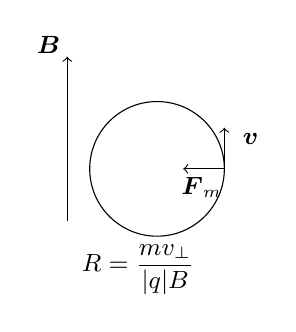
\begin{tikzpicture}[scale=0.95]
  \draw[->] (0,0) -- (0,2.2);
  \node at (-0.25,2.35) {\small \(\vb*{B}\)};
  \draw (1.2,0.7) circle (0.9);
  \draw[->] (2.1,0.7) -- (2.1,1.25);
  \node at (2.45,1.1) {\small \(\vb*{v}\)};
  \draw[->] (2.1,0.7) -- (1.55,0.7);
  \node at (1.8,0.45) {\small \(\vb*{F}_m\)};
  \node at (0.95,-0.65) {\small \(R=\dfrac{mv_\perp}{\abs{q}B}\)};
\end{tikzpicture}
\end{center}

\section{为什么磁力不做功}

磁力不做功的核心并不神秘，只来自一个几何事实：
\[
P=\vb*{F}_m\cdot \vb*{v}
=q(\vb*{v}\times \vb*{B})\cdot \vb*{v}=0.
\]
因为磁力永远垂直于瞬时速度，所以它不能直接增加或减少动能，只能改变速度方向。

\bridge{这句话非常值得反复咀嚼：\textbf{磁场最擅长做的事情不是“加速”粒子，而是“把粒子的运动方向掰弯”。} 以后你看到回旋加速器、质谱仪或电子束偏转，真正起作用的，首先都是“改方向”这一件事。}

\section{洛伦兹力的几个经典应用}

\textbf{速度选择器与质谱仪。} 若带电粒子同时进入互相垂直的电场和磁场，且初速度也与两者都垂直，则当
\[
qE=qvB
\]
时，电场力与磁场力恰好平衡，粒子不发生偏转，于是可选出满足
\[
v=\frac{E}{B}
\]
的那一束粒子。这就是\textbf{速度选择器}。若再让选速后的粒子进入仅有磁场 \(B_0\) 的分析区，它们会做半径为
\[
R=\frac{mv}{|q|B_0}
\]
的圆周运动，因此
\[
\frac{m}{|q|}=\frac{BB_0R}{E}.
\]
于是不同荷质比的粒子就会走出不同半径的轨道，这正是\textbf{质谱仪}区分同位素和测量荷质比的基本思想。

\textbf{汤姆孙实验与电子荷质比。} 阴极射线管中的电子先经电压 \(V\) 加速，因此
\[
\frac12 mv^2=eV.
\]
再让电子束进入互相垂直的电场和磁场，并调到屏上\textbf{不偏转}，则有
\[
eE=evB,
\qquad
v=\frac{E}{B}.
\]
联立两式便得
\[
\frac{e}{m}=\frac{E^2}{2VB^2}.
\]
这条链非常值得记住，因为它告诉你：\textbf{只要能独立控制加速电压、电场和磁场，就能把不可见电子的荷质比测出来。}

\textbf{回旋加速器。} 非相对论带电粒子在匀强磁场中的回旋频率
\[
f=\frac{|q|B}{2\pi m}
\]
与速率无关。因此，只要在两个 D 形盒的缝隙间施加同频交变电场，粒子每次经过缝隙都会被\textbf{电场}再次加速，而\textbf{磁场}只负责把它弯回下一次加速位置。若 D 形盒最大半径为 \(R_0\)，则离开加速器前的最大速率与最大动能约为
\[
v_{\max}=\frac{|q|BR_0}{m},
\qquad
E_{k,\max}=\frac{q^2B^2R_0^2}{2m}.
\]
这里最容易记反的一点是：\textbf{回旋加速器真正负责“增能”的是缝隙中的交变电场，不是磁场。} 磁场只改方向，不改动能。还要注意，这套“频率与速率无关”的结论只在非相对论范围内成立；当粒子速度太高时，相对论效应会让同步条件逐渐失配。

\textbf{磁聚焦（磁透镜）。} 若一束带电粒子从同一点出发，速率近似相同，但与 \(\vb*{B}\) 的夹角 \(\theta\) 都较小且略有差别，那么每个粒子都沿螺旋线前进，其节距为
\[
d=v_\parallel T
=v\cos\theta\frac{2\pi m}{|q|B}.
\]
当 \(\theta\) 都不大时，\(\cos\theta\) 变化不大，各条螺旋线的节距就近似相同，于是粒子束会在后方某处再次会聚。这个现象叫\textbf{磁聚焦}，其本质就是利用洛伦兹力把电子束“整形成像”，所以它在\textbf{电子光学、电子显微镜和电子束控制}中非常重要。

\textbf{霍耳效应。} 在载流导体或半导体中，载流子带着漂移速度 \(v_d\) 前进。若外加磁场垂直于电流方向，载流子会受到横向洛伦兹力，直到横向静电场建立起来并满足
\[
|q|E_H=|q|v_dB,
\qquad
E_H=v_dB.
\]
若试样宽度为 \(b\)、厚度为 \(d\)，则横向霍耳电压大小为
\[
|U_H|=E_Hb=v_dBb.
\]
再由电流大小
\[
I=n|q|v_dbd
\]
可得
\[
|U_H|=\frac{IB}{n|q|d}.
\]
若把载流子电荷符号一并计入霍耳系数，则常写成
\[
U_H=R_H\frac{IB}{d},
\qquad
R_H=\frac{1}{nq}.
\]
因此 \(R_H\) 的\textbf{符号}可以判断主要载流子是正电还是负电，\(R_H\) 的\textbf{大小}又能反推出载流子浓度，霍耳效应也常被用来测磁场。

\section{磁场对载流导线的作用}

导线里有大量定向运动的电荷，所以磁场对载流导线也会施力。若一小段导线元为 \(d\vb*{l}\)，电流为 \(I\)，则
\[
d\vb*{F}=I\,d\vb*{l}\times \vb*{B}.
\]
若导线为直导线且处在匀强磁场中，则总力可简化为
\[
\vb*{F}=I\vb*{L}\times \vb*{B},
\qquad
F=ILB\sin\theta.
\]
之所以还能进一步写成“只看起点和终点”，关键就在于 \(\vb*{B}\) 处处相同：沿路径各小段受力虽然方向不同，但积分时真正累加出来的是整段导线的净位移，所以路径细节会被压扁成端点差。

更一般地，任意一段平面载流导线在匀强磁场中的总力只与起点和终点有关：
\[
\vb*{F}
=I\int d\vb*{l}\times \vb*{B}
=I(\vb*{r}_{\mathrm{end}}-\vb*{r}_{\mathrm{start}})\times \vb*{B}.
\]
于是闭合线圈满足 \(\vb*{r}_{\mathrm{end}}=\vb*{r}_{\mathrm{start}}\)，总力自然为零；这也正是为什么线圈在匀强磁场里更典型的表现不是整体平移，而是受力矩。

这里本质上仍然是洛伦兹力的集体效果：导线中每个载流子都受磁场作用，把这些微观作用沿导线加总，便得到宏观载流导线的受力结果。

\begin{remark}
两根平行载流长直导线之间还会彼此作用：同向电流相吸，反向电流相斥。这个现象本质上就是“一个电流建立磁场，再去作用另一个电流”。
\end{remark}

\section{线圈为什么会被磁场“拧转”}

单根直导线在匀强磁场里往往表现为平移受力；但闭合线圈在匀强磁场里更典型的表现是\textbf{受力矩}。这里最该先有的图像是：\textbf{电流环可以看成一个有朝向的小磁体。} 这个“小磁体想顺着外磁场转过去”的本领，一方面随电流 \(I\) 增大而增大，另一方面随围面积 \(S\) 增大而增大；而它朝向哪边，则只能靠面积法向来记录。于是先用右手定则让四指沿电流方向弯曲，拇指所指的面积法向 \(\vb*{n}\) 就定义了这只电流环的朝向。带着这个图像，再看下面两条式子才不会突兀。\bridge{这里先抓两条结论最省力：\(\vb*{m}=IS\vb*{n}\) 和 \(\vb*{M}=\vb*{m}\times\vb*{B}\)。之所以磁矩自然写成 \(IS\vb*{n}\)，是因为线圈被拧转的趋势同时随电流 \(I\) 和围面积 \(S\) 增大，而线圈正反面的区别又只能靠法向量 \(\vb*{n}\) 来记录。} 对面积为 \(S\)、电流为 \(I\)、法向单位矢量为 \(\vb*{n}\) 的线圈，定义磁矩
\[
\vb*{m}=IS\vb*{n}.
\]
它在匀强磁场中受到的力矩为
\[
\vb*{M}=\vb*{m}\times \vb*{B},
\qquad
M=mB\sin\theta.
\]
若线圈有 \(N\) 匝，则
\[
M=NISB\sin\theta.
\]
这里 \(\theta\) 是线圈法向 \(\vb*{n}\) 与磁场 \(\vb*{B}\) 的夹角，所以 \(\theta=0\) 时是稳定平衡，\(\theta=\pi\) 时是不稳定平衡，\(\theta=\pi/2\) 时力矩最大。

因此线圈总会倾向于把自己的磁矩方向转到与外磁场同向的位置。这个结果和电偶极子在匀强电场中受到力矩非常相似：那边是电偶极矩 \(\vb*{p}\) 想对准 \(\vb*{E}\)，这边是磁矩 \(\vb*{m}\) 想对准 \(\vb*{B}\)。

\begin{remark}
对匀强磁场中的闭合刚性平面线圈，\textbf{合力为零、合力矩一般不为零}。这两个结论要配套记：前者告诉你线圈不必整体飞走，后者告诉你它会被“拧转”到磁矩与外磁场同向的位置。
\end{remark}

\section{磁力对电流回路做功怎样和磁通接起来}

这一节先别把它看成“又来一条新公式”，而应先认出它在回答什么问题：\textbf{当载流回路姿态或位置改变时，磁场对它做的机械功怎样用更统一的量来记？} 既然上一节已经说明线圈受力矩时会自己转去对准磁场，那么下一步最自然的追问就是：这段转动里做了多少功，能不能不用每次都从力矩积分起步？最稳的办法，是先在“匀强磁场中的线圈转动”这个最简单图景里，看力矩做功怎样一步步改写成磁通变化。

若线圈法向与磁场夹角为 \(\theta\)，则磁通量是 \(\Phi_B=BS\cos\theta\)。这时小转角 \(d\theta\) 内的元功满足
\[
dA=M\,d\theta=IBS\sin\theta\,d\theta.
\]
另一方面，
\[
d\Phi_B=d(BS\cos\theta)=-BS\sin\theta\,d\theta.
\]
这里最容易糊掉的是正负号，所以最好先固定一幅图：若线圈当前没有对准外磁场，磁力矩会把它往“磁矩更接近 \(\vb*{B}\)”的方向拧过去；在这个自发转向过程中，\(\theta\) 减小，\(\cos\theta\) 增大，因此磁通 \(\Phi_B=BS\cos\theta\) 增大。与此同时，磁场对回路做正功。也就是说，沿着“磁场自己把线圈拧过去”的实际转向看，\textbf{做正功对应的正是磁通增加。} 在这个约定下，前面两式合起来就可压成
\[
dA=I\,d\Phi_B.
\]
若把功的正负改按“外力对系统做功”来记，或者把法向与转向的约定整体反过来，式子前面的号也会一起改写。所以这里真正要先记的不是孤零零的正负号，而是\textbf{谁在做功、磁通朝哪边变}，再记最后公式。

\begin{remark}
若磁场恒定、电流也恒定，则把上式积分可得磁场对回路所做的功与磁通变化直接挂钩。这一节真正有价值的地方，不是多背一条功公式，而是建立“力矩做功也能回到磁通记账”的统一视角。
\end{remark}

\section{例题精讲}

\begin{exercise}[任意平面载流导线在匀强磁场中的总受力]
在 \(xy\) 平面内，一段任意形状的平滑导线从 \(O(0,0)\) 延伸到 \(P(L,0)\)，导线中通有电流 \(I\)。空间存在垂直纸面向里的匀强磁场 \(\vb*{B}=-B\vb*{k}\)。求整段导线所受总磁场力。
\end{exercise}

\begin{solution}
这题最值得学的不是某个特殊曲线怎么积，而是一个更强的结论：\textbf{在匀强磁场中，平面载流导线的总受力只由始点、终点决定。}

设电流元
\[
d\vb*{l}=dx\,\vb*{i}+dy\,\vb*{j}.
\]
则安培力微元为
\[
d\vb*{F}=I\,d\vb*{l}\times \vb*{B}
=I(dx\,\vb*{i}+dy\,\vb*{j})\times(-B\vb*{k}).
\]
逐项叉乘得
\[
d\vb*{F}=BI\,dx\,\vb*{j}-BI\,dy\,\vb*{i}.
\]
于是
\[
dF_x=-BI\,dy,\qquad dF_y=BI\,dx.
\]
沿整条导线积分：
\[
F_x=-BI\int_O^P dy=0,
\]
因为起点和终点的 \(y\) 坐标都为 \(0\)；
\[
F_y=BI\int_O^P dx=BIL,
\]
因为从 \(x=0\) 走到 \(x=L\)。

故总磁场力为
\[
\vb*{F}=BIL\,\vb*{j}.
\]
也就是说，它恰好等于那根\textbf{从 \(O\) 直连到 \(P\) 的直导线}在同一匀强磁场中所受的力。这是很多安培力积分题里最省力的捷径之一。
\end{solution}

\begin{exercise}[圆形线圈在匀强磁场中的力矩与做功]
半径为 \(R\) 的单匝圆形线圈中通有电流 \(I\)。将它放入匀强磁场中，且初始时磁场方向与线圈平面平行。求：
\begin{enumerate}
  \item 初始时线圈所受磁力矩的大小；
  \item 若线圈在磁力矩作用下转到法向与 \(\vb*{B}\) 同向，磁场力共做多少功。
\end{enumerate}
\end{exercise}

\begin{solution}
对闭合平面线圈，最稳的入口不是逐段算力，而是直接用磁矩
\[
\vb*{m}=IS\,\vb*{n},
\qquad
S=\pi R^2.
\]
初始时磁场与线圈平面平行，故它与法向 \(\vb*{n}\) 的夹角为 \(90^\circ\)。因此总磁力矩大小为
\[
M=mB\sin 90^\circ
=IB\pi R^2.
\]

再看做功。线圈转动时，若电流保持不变，磁力矩所做的功可写成
\[
A=I\Delta\Phi_B.
\]
初始时磁通量
\[
\Phi_i=BS\cos 90^\circ=0,
\]
末态时线圈法向与磁场同向，
\[
\Phi_f=BS\cos 0^\circ=BS=B\pi R^2.
\]
故
\[
A=I(\Phi_f-\Phi_i)=IB\pi R^2.
\]

这题里力矩大小和总做功恰好写成了同一个系数 \(IB\pi R^2\)，但它们的物理意义完全不同：前者是某一姿态下的“转动趋势”，后者是整个转动过程中“累计转移的能量”。
\end{solution}

\begin{exercise}[长直载流导线在匀强磁场中的受力]
一段长为 \(L\) 的直导线中通有电流 \(I\)，置于匀强磁场 \(\vb*{B}\) 中。若导线方向与磁场夹角为 \(\theta\)，求导线所受安培力。
\end{exercise}

\begin{solution}
对直导线，安培力微元
\[
d\vb*{F}=I\,d\vb*{l}\times \vb*{B}.
\]
由于整段导线方向固定、磁场又均匀，大小可以直接积出来：
\[
F=\int I B\sin\theta\,dl
=IB\sin\theta\int_0^L dl.
\]
因此
\[
\boxed{F=ILB\sin\theta}.
\]
方向由 \(I\vb*{L}\times \vb*{B}\) 决定。这个式子其实就是安培力最常见的整段导线版，后面很多复杂导线题都只是把它拆回微元再积分。
\end{solution}

\begin{exercise}[有限长直导线受无限长直导线的磁场力]
一根无限长直导线中通有电流 \(I_1\)。与它共面地放置一根长为 \(L\) 的直导线，电流为 \(I_2\)。设该导线近端到长直导线的距离为 \(r\)，并与过近端的垂线夹角为 \(\alpha\)。求这根有限导线所受磁场力大小。
\end{exercise}

\begin{solution}
长直导线在距其 \(x\) 处产生的磁场大小为
\[
B(x)=\frac{\mu_0I_1}{2\pi x}.
\]
有限导线上的每一小段所受安培力方向相同，因此只需积分大小。由几何关系
\[
x=r+l\cos\alpha,
\qquad
dl=\frac{dx}{\cos\alpha}.
\]
于是
\[
dF=I_2B(x)\,dl
=\frac{\mu_0I_1I_2}{2\pi x}\frac{dx}{\cos\alpha}.
\]
从 \(x=r\) 积到 \(x=r+L\cos\alpha\)，得
\[
F=\frac{\mu_0I_1I_2}{2\pi\cos\alpha}\int_r^{r+L\cos\alpha}\frac{dx}{x}
=\frac{\mu_0I_1I_2}{2\pi\cos\alpha}\ln\frac{r+L\cos\alpha}{r}.
\]
故
\[
\boxed{
F=\frac{\mu_0I_1I_2}{2\pi\cos\alpha}\ln\frac{r+L\cos\alpha}{r}
}.
\]
这题的难点纯粹是几何变量替换，本质仍是“先找外磁场，再对安培力积分”。
\end{solution}

\begin{exercise}[半圆形载流导线在匀强磁场中的受力]
半径为 \(R\) 的半圆形导线位于纸面内，电流沿圆弧从左端流向右端，空间有垂直纸面向里的匀强磁场 \(B\)。求该半圆弧所受总安培力。
\end{exercise}

\begin{solution}
逐元积分固然可做，但更快的识别是：在匀强磁场中，一段平面载流导线的总受力只由起点和终点决定。因此该半圆弧受到的总力，等于连接两端的直径导线在同一磁场中的受力。

于是直接得
\[
F=IB(2R).
\]
故
\[
\boxed{F=2IBR}.
\]
方向由电流方向与磁场方向的叉乘决定；按题设取向，它与直径垂直并指向半圆开口一侧。这个结果很好地说明了“匀强磁场里算整段导线受力，别总想着沿曲线死积分”。
\end{solution}

\begin{exercise}[圆形线圈在指定坐标系中的磁力矩方向]
一半径为 \(R\) 的可转动圆形线圈中通有电流 \(I\)，线圈法向沿 \(+z\) 方向，匀强磁场 \(\vb*{B}=B\vb*{i}\)。求线圈所受磁力矩。
\end{exercise}

\begin{solution}
线圈磁矩为
\[
\vb*{m}=IS\,\vb*{k}=I\pi R^2\,\vb*{k}.
\]
所以
\[
\vb*{M}=\vb*{m}\times \vb*{B}
=I\pi R^2\,\vb*{k}\times B\vb*{i}
=I\pi R^2B\,\vb*{j}.
\]
故
\[
\boxed{\vb*{M}=I\pi R^2B\,\vb*{j}}.
\]
这题提醒我们：很多线圈受力矩题真正的关键不是大小，而是先把磁矩方向判对，再用叉乘一把得到方向。
\end{solution}

\begin{exercise}[圆电流与共面长直导线间的安培力]
一根无限长直导线与半径为 \(R\)、电流为 \(I\) 的圆电流共面放置，并沿圆的一条直径方向通过。长直导线电流为 \(I_0\)。求：
\begin{enumerate}
  \item 圆上半弧所受总安培力；
  \item 整个圆电流所受总安培力。
\end{enumerate}
\end{exercise}

\begin{solution}
对位于半圆弧上的电流元，长直导线在其处产生的磁场大小为
\[
B=\frac{\mu_0 I_0}{2\pi x},
\]
其中 \(x=R\sin\theta\)。把安培力微元分解后，由对称性可知垂直于直径的分量相互抵消，只剩沿直径方向的分量。积分结果为
\[
F_{\text{半弧}}=\frac{\mu_0 I_0 I}{2}.
\]
而对整个圆电流，同样的积分在上下两半圆上同向叠加，因此
\[
F_{\text{全圆}}=\mu_0 I_0 I.
\]
故
\[
\boxed{
F_{\text{半弧}}=\frac{\mu_0 I_0 I}{2},
\qquad
F_{\text{全圆}}=\mu_0 I_0 I.
}
\]
这类题看起来像“奇怪几何”，本质还是两步：先写出长直导线的磁场，再利用对称性删去会互相抵消的分量。
\end{solution}

\section{本章统一起手动作}

涉及磁场力时，最稳的顺序是：
\begin{enumerate}
  \item 先看研究对象：单个电荷、整段导线，还是闭合线圈；
  \item 再看 \(\vb*{v}\) 或 \(d\vb*{l}\) 与 \(\vb*{B}\) 的夹角；
  \item 然后先画方向图，再代数计算大小；
  \item 一旦题目问能量或速率变化，立刻回想“磁力不做功”，看它到底能改什么、不能改什么。
\end{enumerate}

\section{常见误区}

\begin{itemize}
  \item 把磁力方向错画成沿 \(\vb*{v}\) 或沿 \(\vb*{B}\)。
  \item 误以为“只要有磁力就一定会越来越快”。磁力改方向，不直接改动能。
  \item 把载流导线受力和平行导线相互作用混成两套无关公式，忘了它们都来自 \(I\,d\vb*{l}\times \vb*{B}\)。
  \item 看到线圈就只算总力，忽略真正支配转动的是力矩。
\end{itemize}

\section{章末小结}

\summaryline{磁场对运动电荷的作用由洛伦兹力给出，它总垂直于速度，所以最擅长“拐弯”而不是“增速”；速度选择器、质谱仪、汤姆孙实验、回旋加速器和霍耳效应都只是这同一条力学主线在不同装置中的展开；对载流导线，微观洛伦兹力加总成宏观磁场力；对闭合线圈，又进一步表现为磁矩在外磁场中的受力矩。}
\chapterselfcheck{为什么匀强磁场能让粒子做圆周或螺旋运动，却不直接改动能？为什么回旋加速器里真正负责增加动能的是电场而不是磁场？为什么霍耳电压的符号能判断载流子类型？遇到电子在磁场中偏转的题，为什么一定要先画方向图？}

\chapter{磁介质}

\begin{skill}[第18章冲刺总手册]\label{sk:phys-ch18-overview}
\textbf{【这章先解决什么题】} 这章处理“材料放进磁场后，外磁场和介质自身响应怎样分账”的题。核心不是再造一套新力学，而是把 \(\vb*{B},\vb*{H},\vb*{M}\) 各自管什么说清。
\textbf{【拿题先认什么信号】} 题面若出现“磁化强度、磁介质、顺磁、抗磁、铁磁、自由电流、束缚电流、磁化电流、磁场强度”，就说明题目要你区分“外部电流造成的场”和“介质被磁化后的附加响应”。
\textbf{【第一条方程先写什么】}
\[
\begin{aligned}
\oint_L \vb*{H}\cdot \dd \vb*{l}&=I_{\mathrm{free}},\\
\vb*{B}&=\mu_0(\vb*{H}+\vb*{M}).
\end{aligned}
\]
先用 \(\vb*{H}\) 盯住自由电流，再用 \(\vb*{M}\) 把介质响应补回到 \(\vb*{B}\)。
\textbf{【必背公式块】}
\[
\begin{aligned}
\vb*{B}&=\mu_0(\vb*{H}+\vb*{M}),\\
\vb*{M}&=\chi_{\mathrm m}\vb*{H}
\quad \text{(线性各向同性磁介质)},\\
\vb*{B}&=\mu \vb*{H}
=\mu_0(1+\chi_{\mathrm m})\vb*{H}
=\mu_r\mu_0\vb*{H},\\
\oint_L \vb*{H}\cdot \dd \vb*{l}&=I_{\mathrm{free}},\qquad
\oint_S \vb*{B}\cdot \dd \vb*{S}=0.
\end{aligned}
\]
这里 \(\chi_{\mathrm m}\) 是磁化率，\(\mu_r\) 是相对磁导率；\(\vb*{H}\) 主要追踪自由电流，\(\vb*{B}\) 才是最后真正参与受力和磁通量的场。
\textbf{【做题流程】} 先看题目给的是自由电流、总磁感应强度还是材料参数；若几何对称明显，先用 \(\oint \vb*{H}\cdot\dd\vb*{l}=I_{\mathrm{free}}\) 求 \(\vb*{H}\)；再由材料关系求 \(\vb*{M}\) 或 \(\vb*{B}\)。若题目只在讨论磁介质前后同一装置中场的变化，就重点比较 \(\mu_r\) 进入后哪些量按比例变化。
\textbf{【最容易误判】} 把 \(\vb*{H}\) 和 \(\vb*{B}\) 当成完全等价；见到介质后仍直接把安培环路定理写成 \(\oint \vb*{B}\cdot \dd\vb*{l}=\mu_0 I_{\mathrm{free}}\) 而不交代条件；把顺磁、抗磁的差别记反；忘记磁介质里仍满足 \(\nabla\cdot \vb*{B}=0\)。
\textbf{【最后怎样验证】} 看结果是否符合材料直觉：顺磁或铁磁应增强同向磁感应，抗磁应减弱；看无介质极限 \(\mu_r\to 1\) 时是否回到真空结果；量纲上 \(\vb*{B}\) 是 \(\mathrm T\)，\(\vb*{H}\) 是 \(\mathrm{A/m}\)，不要混写。
\end{skill}

\chapterroadmap
{回答“物质进入磁场后怎样被磁化”，并把 \(\vb*{B},\vb*{H},\vb*{M}\) 三个量的分工理顺。}
{已经知道电流建立磁场、磁场作用于运动电荷和电流。}
{新增磁化、磁化电流、磁场强度 \(\vb*{H}\)、介质中的安培环路定理，以及抗磁/顺磁/铁磁的差异。}

\bridge{静电学里，电介质进入外场会极化；磁学里，磁介质进入外场会磁化。于是 \(\vb*{B}\) 不再只由自由电流决定，还会受到介质内部微观磁矩取向变化的影响。学这一章的关键，就是把“自由电流造的那部分场”和“介质自己响应出来的那部分场”分开记账。}

\section{磁化与磁矩}

前面一直在宏观上讨论“外部电流怎样造场”；下面为了说明材料为什么会自己补出一份磁场，必须暂时切到微观磁矩图像。

从微观上看，很多原子、分子或电子轨道本身就可等效为小电流环。只要有电流环，就会自然带有磁矩：
\[
\vb*{m}=IS\,\vb*{n},
\]
其中 \(I\) 是等效环流，\(S\) 是环面积，方向 \(\vb*{n}\) 由右手定则给出。也就是说，磁矩并不是凭空冒出来的抽象矢量，而是在把“这一小圈电流想把自己朝哪边摆”浓缩成一个方向和大小。没有外磁场时，这些微观磁矩往往取向杂乱，宏观平均后磁效应不明显；加上外磁场后，部分磁矩趋于定向排列，宏观上就表现为磁化。

磁化强度记作 \(\vb*{M}\)，它描述单位体积内净磁矩的平均分布，可写成
\[
\vb*{M}=\frac{d\vb*{m}}{dV}.
\]
虽然教材上它看起来只是“又一个新矢量”，但物理意义非常明确：\textbf{它刻画的是介质内部自己贡献出来的磁性部分。} 若把介质想成许多微观小电流环排队，\(\vb*{M}\) 就是在记“这些小电流环到底排得有多整齐、总体更偏向哪边”。

\bridge{若把磁化想成大量微观小电流环重新排队，就会发现一个很关键的几何事实：相邻小电流环在内部边界上的电流会彼此抵消，真正留下来的主要是外表面的等效环流。因此磁化不仅可以用“磁矩取向”来讲，也可以用“等效磁化电流”来讲。}

\begin{note}
\textbf{记方向时最稳的办法是先想右手定则：} 四指沿等效环流方向弯过去，大拇指所指就是磁矩方向，也是宏观磁化强度 \(\vb*{M}\) 的方向。这样就不会把“磁矩指向”和“电流绕行方向”混成两套互不相干的规定。
\end{note}

真正做题时，并不是要把所有微观电流逐个算出来，而是把一束平行排开的微观电流环粗略打包：回路真正统计到的是净剩下的边界环流，所以才会出现“\(\vb*{M}\) 的环量 = 围住的等效电流”这类关系。

若取一条闭合回路 \(L\) 围住介质的一部分，则磁化强度与等效磁化电流满足
\[
\oint_L \vb*{M}\cdot d\vb*{l}=\sum I_s,
\]
这里 \(\sum I_s\) 表示被回路围住的等效磁化电流代数和。这个关系的价值在于：它把抽象的 \(\vb*{M}\) 重新翻译回了我们已经熟悉的“电流造磁场”语言。

\section{磁场强度 H 与介质中的安培环路定理}

这里第一次最容易卡的是：明明已经有了 \(\vb*{B}\) 和 \(\vb*{M}\)，为什么又要再来一个 \(\vb*{H}\)？最稳的想法是先把目标说死：\textbf{若题目要你按自由电流来写环路定理，就必须有一个量能把磁化那一部分先剥出去。} 这时三者分工就清楚了：\(\vb*{M}\) 记的是材料自身磁化，也就是“单位体积净磁矩”；\(\vb*{B}\) 记的是最后真正参与受力、决定磁通的总磁场；\(\vb*{H}\) 则像静电学里的 \(\vb*{D}\) 一样，是为了把\textbf{自由电流源单独拎出来记账}而引入的辅助场。为了把“自由电流贡献”和“磁化贡献”分账，引入磁场强度 \(\vb*{H}\)。在真空中，
\[
\vb*{B}=\mu_0\vb*{H};
\]
在一般介质中，
\[
\vb*{B}=\mu_0(\vb*{H}+\vb*{M}).
\]
它不是凭空多造一个字母，而是从“总环量怎样拆账”这件事里被逼出来的。因为介质中
\[
\oint_L \vb*{B}\cdot d\vb*{l}
=\mu_0\left(\sum I_{\mathrm{free}}+\sum I_s\right)
=\mu_0\left(\sum I_{\mathrm{free}}+\oint_L \vb*{M}\cdot d\vb*{l}\right).
\]
既然右边第二项正是“介质自己响应出来的那本账”，那就把它移到左边，让左边只剩自由电流对应的部分，于是
\[
\vb*{H}=\frac{\vb*{B}}{\mu_0}-\vb*{M},
\qquad
\oint_L \vb*{H}\cdot d\vb*{l}=I_{\mathrm{free}}.
\]
对各向同性线性均匀磁介质，还可以进一步写成
\[
\vb*{M}=\chi_m \vb*{H},
\qquad
\vb*{B}=\mu\vb*{H},
\]
其中 \(\mu=\mu_0(1+\chi_m)\) 为磁导率。

于是安培环路定理在介质中最实用的写法变成
\[
\oint_L \vb*{H}\cdot d\vb*{l}=I_{\mathrm{free}}.
\]

\begin{note}
\textbf{这和电介质里引入 \(\vb*{D}\) 的思路完全平行：} \(\vb*{B}\) 对总磁效应负责，\(\vb*{H}\) 主要对自由电流负责。以后只要介质一出现，就不要再把真空中的单一本构关系机械照搬。
\end{note}

\section{三类常见磁介质：抗磁、顺磁、铁磁}

\bridge{这一节最怕被读成名词表。更自然的起手是先看材料内部的小磁矩在外场来之前和来了之后分别会怎样：有的材料本来几乎没有可稳定排队的永久磁矩，只会被外场轻微诱导反向响应；有的本来就有微观磁矩，但只能弱弱地顺着外场多排一点；还有的内部早就分成一块块磁畴，外场一来会成片翻转，甚至留下明显历史记忆。也正因为微观机制不同，宏观上才会分成抗磁、顺磁和铁磁三类。}

\begin{itemize}
  \item \textbf{抗磁质：} 外场使感生磁矩方向与外场相反，磁化很弱，\(\mu_r\) 略小于 1。
  \item \textbf{顺磁质：} 原有磁矩在外场中略趋同向，磁化较弱，\(\mu_r\) 略大于 1。
  \item \textbf{铁磁质：} 内部存在磁畴结构，外场可使磁畴大范围重排，因此磁化很强，\(\mu_r\) 可远大于 1。
\end{itemize}

铁磁质之所以特殊，不只是“磁化更大”，而是它具有明显的历史效应：外场撤去后，磁化不一定立刻完全消失，于是出现剩磁、矫顽力和磁滞回线等现象。

\section{磁滞与软磁、硬磁材料}

铁磁材料里，\(\vb*{B}\) 与 \(\vb*{H}\) 之间常不再是一条简单直线，而是随加磁、退磁历史出现磁滞回线。回线窄、矫顽力小的材料适合做铁芯等反复磁化退磁的器件，常称\textbf{软磁材料}；回线宽、剩磁大的材料适合做永久磁体，常称\textbf{硬磁材料}。

\begin{remark}
这里最容易被忽略的是：铁磁质不是“\(\mu\) 特别大”的单纯线性介质，而是一类具有磁畴结构、非线性和历史记忆效应的材料。
\end{remark}

\section{例题精讲}

\begin{exercise}[\(H\) 与 \(B\) 的分段分工]
一半径为 \(R_1\) 的无限长圆柱导线外包一层外半径为 \(R_2\)、相对磁导率为 \(\mu_r\) 的均匀磁介质圆筒。导线中通有电流 \(I\)，且电流在导线截面上均匀分布。求各区域中的磁场强度 \(H(r)\) 与磁感应强度 \(B(r)\)。
\end{exercise}

\begin{solution}
这题最关键的观念不是一上来就算 \(B\)，而是先记住：\textbf{\(\vb*{H}\) 主要由自由电流决定，\(\vb*{B}\) 再由介质响应放大或缩小。}

先用半径为 \(r\) 的圆形安培回路。由对称性，\(\vb*{H}\) 沿回路切向且大小恒定，于是
\[
\oint \vb*{H}\cdot d\vb*{l}=H(2\pi r)=I_{\mathrm{free,enc}}.
\]

当 \(0<r<R_1\) 时，包围的自由电流仅占总电流的面积比：
\[
I_{\mathrm{enc}}=I\frac{r^2}{R_1^2}.
\]
故
\[
H(r)=\frac{Ir}{2\pi R_1^2},
\qquad
B(r)=\mu_0H(r)=\frac{\mu_0Ir}{2\pi R_1^2}.
\]
这里仍在导线本体内部，尚未进入外包磁介质，所以 \(B=\mu_0H\)。

当 \(R_1<r<R_2\) 时，回路已包围全部自由电流 \(I\)，因此
\[
H(r)=\frac{I}{2\pi r}.
\]
但这一区域位于磁介质中，所以
\[
B(r)=\mu H(r)=\mu_0\mu_r\frac{I}{2\pi r}.
\]

当 \(r>R_2\) 时，回路外侧回到真空（或空气），包围自由电流仍是 \(I\)，所以
\[
H(r)=\frac{I}{2\pi r},
\qquad
B(r)=\mu_0\frac{I}{2\pi r}.
\]

综上，
\[
H(r)=
\begin{cases}
\dfrac{Ir}{2\pi R_1^2}, & 0<r<R_1,\\[6pt]
\dfrac{I}{2\pi r}, & r>R_1,
\end{cases}
\]
\[
B(r)=
\begin{cases}
\dfrac{\mu_0Ir}{2\pi R_1^2}, & 0<r<R_1,\\[6pt]
\dfrac{\mu_0\mu_rI}{2\pi r}, & R_1<r<R_2,\\[6pt]
\dfrac{\mu_0I}{2\pi r}, & r>R_2.
\end{cases}
\]

这正体现了 \(\vb*{H}\) 与 \(\vb*{B}\) 的分工：\(\vb*{H}\) 先把自由电流的“源账”做好，\(\vb*{B}\) 再通过不同区域的本构关系体现介质影响。
\end{solution}

\begin{exercise}[充满磁介质的长直螺线管]
一长直密绕螺线管内充满相对磁导率为 \(\mu_r\) 的均匀磁介质，单位长度匝数为 \(n\)，通有电流 \(I\)。求管内磁感应强度。
\end{exercise}

\begin{solution}
先对 \(\vb*{H}\) 用安培环路定理。取一条跨越螺线管内外的矩形回路，由于长螺线管外部磁场近似很小，内部 \(\vb*{H}\) 近似均匀，故
\[
Hl=nIl
\quad\Longrightarrow\quad
H=nI.
\]
再由线性磁介质中的本构关系
\[
B=\mu H=\mu_0\mu_r H
\]
得到
\[
\boxed{
B=\mu_0\mu_r nI
}.
\]
这题最能说明“先算 \(H\)，再转成 \(B\)”的好处：自由电流决定 \(H\)，介质参数只在最后一步进入。
\end{solution}

\begin{exercise}[两同轴反向电流圆筒间的磁场]
有两个半径分别为 \(R_1,R_2\) 的无限长同轴圆筒形导体，之间充满相对磁导率为 \(\mu_r\) 的均匀磁介质。两圆筒中通有大小相等、方向相反的电流 \(I\)。求各区域磁感应强度。
\end{exercise}

\begin{solution}
对三段区域分别用安培环路定理求 \(\vb*{H}\)：

当 \(r<R_1\) 时，回路不包围净自由电流，故
\[
H=0,\qquad B=0.
\]

当 \(R_1<r<R_2\) 时，回路只包围内圆筒电流 \(I\)，故
\[
H\cdot 2\pi r=I
\quad\Longrightarrow\quad
H=\frac{I}{2\pi r}.
\]
此区在磁介质内，所以
\[
B=\mu_0\mu_r H
=\frac{\mu_0\mu_r I}{2\pi r}.
\]

当 \(r>R_2\) 时，回路同时包围 \(+I\) 和 \(-I\)，净自由电流为零，因此
\[
H=0,\qquad B=0.
\]
故
\[
\boxed{
B(r)=
\begin{cases}
0, & r<R_1,\\[4pt]
\dfrac{\mu_0\mu_r I}{2\pi r}, & R_1<r<R_2,\\[6pt]
0, & r>R_2.
\end{cases}}
\]
它和同轴电缆的电场分布非常像，只不过这里是磁场，而且由反向电流把场锁在两圆筒之间。
\end{solution}

\section{本章统一起手动作}

磁介质题最稳的起手顺序通常是：
\begin{enumerate}
  \item 先问题目是在\textbf{算场}，还是在\textbf{认材料行为}；
  \item 若是算场，先把自由电流与介质响应分账：优先用
  \[
  \oint \vb*{H}\cdot d\vb*{l}=I_{\mathrm{free}}
  \]
  去锁自由电流贡献，再回到 \(\vb*{M}\) 与 \(\vb*{B}\)；
  \item 若介质可近似看作线性、各向同性、均匀介质，就顺着
  \[
  \vb*{M}=\chi_m\vb*{H},
  \qquad
  \vb*{B}=\mu\vb*{H}
  \]
  这条链往下走；
  \item 若题目谈的是铁磁质、磁滞、剩磁、矫顽力，就不要再把它当成“\(\mu\) 很大的线性材料”，而应切到磁畴与历史效应的语言。
\end{enumerate}

\begin{note}
\textbf{这一章最值得死记的不是某个单独公式，而是三者分工：} \(\vb*{B}\) 描写总磁效应，\(\vb*{H}\) 主要对自由电流记账，\(\vb*{M}\) 描写介质自己的磁化响应。很多介质题一旦把这三者混成一个量，后面几乎必乱。
\end{note}

\section{常见误区}

\begin{itemize}
  \item 把 \(\vb*{B}\) 和 \(\vb*{H}\) 当成同一个量，只差一个单位。
  \item 在介质题里仍然机械使用真空关系 \(B=\mu_0H\)。
  \item 以为顺磁、抗磁、铁磁的区别只是“强弱不同”，忽略铁磁质的磁畴和磁滞特性。
  \item 以为磁化意味着材料内部真的有宏观电荷流在绕圈跑；更准确地说，它是微观磁矩平均取向变化的宏观表述。
\end{itemize}

\section{章末小结}

\summaryline{磁介质进入外磁场后会磁化，于是磁场分成“自由电流建立的部分”和“介质响应建立的部分”两本账。用 \(\vb*{H}\) 可以更方便地追踪前者，用 \(\vb*{M}\) 则描述后者；而铁磁质之所以特殊，关键在于磁畴重排和磁滞。}
\chapterselfcheck{为什么介质题里要把 \(\vb*{B}\)、\(\vb*{H}\)、\(\vb*{M}\) 分开？为什么铁磁质不能简单看成“\(\mu\) 很大的线性介质”？为什么介质中的安培环路定理更适合写成关于 \(\vb*{H}\) 的形式？}

\chapter{电磁感应}

\begin{skill}[第19章冲刺总手册]\label{sk:phys-ch19-overview}
\textbf{【这章先解决什么题】} 这章解决“为什么回路里会自己冒出电动势”的题。所有入口都围绕一个判断：磁通量为什么变了，是磁场变、面积变、姿态变，还是导体在切割磁感线。
\textbf{【拿题先认什么信号】} 题面若出现“线圈穿过磁场”“磁通量变化”“感应电流方向”“导杆滑动”“自感、互感”“回路中电流随时间变化”，先把“谁导致磁通变化”圈出来。
\textbf{【第一条方程先写什么】}
\[
\begin{aligned}
\Phi_B&=\int_S \vb*{B}\cdot \dd \vb*{S},\\
\mathcal{E}&=-\dv{\Phi_B}{t}.
\end{aligned}
\]
先找磁通量，再谈符号；楞次定律本质上就是这个负号的物理解释。
\textbf{【必背公式块】}
\[
\begin{aligned}
\Phi_B&=\int_S \vb*{B}\cdot \dd \vb*{S}
\ \Rightarrow\ 
\Phi_B=BS\cos\theta\ \text{(匀强磁场平面回路)},\\
\mathcal{E}&=-\dv{\Phi_B}{t},\qquad
\mathcal{E}_{\text{动生}}=Blv\ \text{(导杆垂直切割时)},\\
\mathcal{E}_L&=-L\dv{I}{t},\qquad
\mathcal{E}_{21}=-M\dv{I_1}{t},\\
W_m&=\frac12 LI^2.
\end{aligned}
\]
其中 \(L\) 是自感系数，\(M\) 是互感系数；动生电动势公式 \(Blv\) 只是法拉第定律在特定几何下的短写。
\textbf{【做题流程】} 先明确回路和取正方向，再写 \(\Phi_B\)；接着判断通量变化来自 \(B,S,\theta\) 哪一个，必要时把 \(\Phi_B=BS\cos\theta\) 分别对时间求导；然后用楞次定律判感应电流方向，最后再联立欧姆定律或回路方程求电流、功率、外力。遇到自感题，直接把 \(-L\dfrac{\dd I}{\dd t}\) 写进回路方程。
\textbf{【最容易误判】} 一上来背楞次定律口号，却没先说明磁通到底怎样变化；把磁通量变化误当成只看 \(B\) 变化；动生电动势里速度方向、导杆方向、磁场方向三者不互相垂直时仍机械套 \(Blv\)；把自感电动势方向写成“总是与电流反向”，其实它反抗的是电流变化。
\textbf{【最后怎样验证】} 看感应效应是否真的阻碍原变化：磁通增大时感应磁场应设法减小它，磁通减小时感应磁场应设法补回来；量纲上电动势是伏特；若导杆做匀速切割，外力做功应与回路发热或电磁能增加对应上。
\end{skill}

\chapterroadmap
{把“变化的磁场”与“感应电动势”接起来，理解法拉第定律、楞次定律、动生/感生电动势，以及自感、互感和磁场能量。}
{已经会描述稳恒电流和静磁场，也知道磁场对电荷和电流的作用。}
{新增磁通量、法拉第电磁感应定律、非静电力场、自感/互感与磁场能量。}

\bridge{前面磁学讨论的大多是“电流产生磁场、磁场作用电流”；这一章出现真正的双向耦合：变化的磁场反过来又能生电场和电流。法拉第定律因此是电磁学从“静态章节并列”走向“动态统一理论”的关键转折。}

\section{磁通量与法拉第电磁感应定律}

这一节真正该先想清楚的是：回路里出现感应电流，不是因为“磁场神秘地产生了电”，而是因为\textbf{穿过回路的总磁场联系正在变化}。若回路所围面积、姿态、或空间磁场本身随时间变了，那么“回路和磁场的联系量”就不再固定，于是系统会用感应电动势来反抗这种变化。这个“联系量”就是磁通。

穿过某曲面的磁通量定义为
\[
\Phi_B=\int_S \vb*{B}\cdot d\vb*{S}.
\]
若回路所围曲面的磁通量随时间变化，则回路中会出现感应电动势：
\[
\mathcal{E}=-\dv{\Phi_B}{t}.
\]
这就是\textbf{法拉第电磁感应定律}。

这里的负号不是装饰，而是\textbf{楞次定律}的数学体现：感应电流总要反抗原磁通变化。若原磁通在增大，感应电流建立的磁场就倾向于让它减小；若原磁通在减小，感应电流就倾向于把它“补回来”。

\begin{remark}
真正判断方向时，最稳的做法是：\textbf{先任选回路绕行方向，再按右手螺旋给穿过回路的磁通规定正方向。} 若算得 \(\mathcal{E}>0\)，说明感应电动势方向与所选绕向一致；若算得 \(\mathcal{E}<0\)，则实际方向与所选绕向相反。这样负号就不再神秘，而是清楚地落实到方向约定上。
\end{remark}

若线圈有 \(N\) 匝，更自然的记账量是\textbf{磁通链}
\[
\Psi=N\Phi_B,
\qquad
\mathcal{E}=-\dv{\Psi}{t}.
\]

\section{动生电动势与感生电动势}

在写公式前，最好先把两种来源分开：若是导体自己在磁场里切割磁感线，真正推动电荷的是载流子随导体运动时受到的洛伦兹力，这叫动生；若导体不动但磁场自己在变，则空间里会出现环形感应电场去推电荷，这叫感生。两种机制的表面现象都叫“有感应电动势”，但第一推手并不是同一个。

磁通变化有两种典型来源：
\begin{itemize}
  \item 回路本身在磁场中运动或形变，这时常称\textbf{动生电动势}；
  \item 回路不动，但空间磁场随时间变化，这时常称\textbf{感生电动势}。
\end{itemize}

对长度为 \(l\) 的金属棒以速度 \(v\) 垂直切割匀强磁场时，有经典结果
\[
\mathcal{E}=Blv.
\]
更一般地，动生电动势可写成
\[
\mathcal{E}=\int (\vb*{v}\times \vb*{B})\cdot d\vb*{l}.
\]
而感生电动势的本质，则是变化磁场激发了非静电感应电场，使得沿闭合回路
\[
\oint \vb*{E}_{\mathrm{ind}}\cdot d\vb*{l}=-\dv{\Phi_B}{t}.
\]

\begin{exercise}
设半径为 \(R\) 的长螺线管内部磁场 \(B(t)\) 近似均匀，管外磁场近似忽略。若取与轴同心、半径为 \(r\) 的圆形回路，则感生电场沿环向分布，并满足
\[
2\pi r E_\varphi=-\pi r^2\dv{B}{t},
\qquad r<R,
\]
故
\[
E_\varphi(r)=-\frac{r}{2}\dv{B}{t}.
\]
若 \(r>R\)，穿过回路的磁通只由半径 \(R\) 的内部磁场决定，于是
\[
2\pi r E_\varphi=-\pi R^2\dv{B}{t},
\qquad
E_\varphi(r)=-\frac{R^2}{2r}\dv{B}{t}.
\]
这说明感生电场并不只存在于“有磁场的地方”，而是以闭合场线的形式分布在更广的空间区域中。换句话说，它的电场线不是从正电荷出发、到负电荷终止，而是绕着变化磁通围成一圈圈与螺线管同轴的闭合同心圆。
\end{exercise}

\begin{remark}
动生电动势的“非静电力来源”可以直接追到洛伦兹力；感生电动势则更深一步，说明即使没有导体整体运动，变化磁场本身也能在空间中建立有旋电场。
\end{remark}

\begin{remark}
也正因为感生电场本身就真实存在，所以即使导体整体静止、甚至不是完整闭合回路，导体两端也可能测得感应电动势；若把大块导体放入时变磁场中，内部还会自动围成许多闭合感应电流回路，这就是\textbf{涡电流}。它一方面会带来额外焦耳热，另一方面又能产生电磁阻尼，所以工程上常通过叠片、开槽等方式削弱涡流回路面积。
\end{remark}

\section{自感与互感}

这一节读公式前最重要的一句判断是：电流变化最先改写的是磁通，而磁通变化又会反过来阻碍这种电流变化本身。所以无论自感还是互感，本质上都不是“突然多了一个常数 \(L\) 或 \(M\)”，而是“电流 \(\rightarrow\) 磁通 \(\rightarrow\) 反向感应电动势”这条回路被压成了比例关系。

如果同一回路中的电流变化引起本回路磁通变化，就会在自身回路中产生感应电动势，这叫\textbf{自感}。更严谨地说，应先定义磁通链 \(\Psi\)，再写
\[
\Psi=LI,
\qquad
\mathcal{E}_L=-L\dv{I}{t}.
\]
若线圈有 \(N\) 匝，则 \(\Psi=N\Phi_B\)。只有在单匝或已默认按磁通链记账时，才可把它简写成“\(\Phi\) 与 \(I\) 成正比”的样子。

若一个回路中的电流变化，引起另一个回路中磁通变化并产生感应电动势，则叫\textbf{互感}。同样应先写成
\[
\Psi_{21}=MI_1,
\qquad
\mathcal{E}_{21}=-M\dv{I_1}{t}.
\]

\begin{note}
自感和互感的核心物理意义都是“电流变化引起磁通变化，再由磁通变化反过来阻碍这种变化”。这也是为什么很多电感元件表现出“电流不愿突然变化”的惯性。
\end{note}

\section{磁场能量}

这里先别把 \(W_m=\frac12 LI^2\) 当成又一条孤立结果。真正该先想的是：建立电流时，外界明明在持续对抗自感电动势做功，而一旦电流稳定后，这部分功并没有凭空消失，只能被储存在某个地方。电磁学前面已经反复提醒过我们，能量不只贴在粒子或元件上，也可以分布在空间中的场里。所以磁场能量公式本质上是在回答：\textbf{刚才那部分克服自感做下去的功，最后记到了磁场账上。}

建立电流要克服自感电动势，因此外界做功会储存在磁场中。对电感元件，
\[
W_m=\frac{1}{2}LI^2.
\]
若进一步写成场的形式，在真空中常用
\[
w_m=\frac{B^2}{2\mu_0},
\]
在一般线性介质中则更自然地写成
\[
w_m=\frac{1}{2}\vb*{B}\cdot \vb*{H}.
\]

\bridge{电场里有 \(\frac12 \vb*{E}\cdot \vb*{D}\)，磁场里有 \(\frac12 \vb*{B}\cdot \vb*{H}\)。这再次提醒我们：电磁学越来越倾向于把能量理解成\textbf{场分布}，而不是只贴在元件或粒子本身。}

\section{例题精讲}

\begin{exercise}[滑动导杆的感应电动势]
矩形闭合导体回路的一边 \(ab\) 长为 \(l\)，可在导轨上无摩擦滑动。整个回路处在垂直于回路平面、大小为 \(B\) 的匀强磁场中。若导杆 \(ab\) 以恒定速度 \(v\) 向右滑动，求回路中的感应电动势。
\end{exercise}

\begin{solution}
这类题最稳的入口不是背 \(Blv\)，而是先把它翻译成“\textbf{磁通为什么在变}”。这里 \(B\) 不变，夹角不变，真正变化的是回路面积。

设时刻 \(t\) 时导杆位置对应回路宽度为 \(x\)，取顺时针绕行为正，则穿过回路的磁通量为
\[
\Phi_B=BS=Blx.
\]
于是
\[
\mathcal{E}=-\dv{\Phi_B}{t}
=-Bl\dv{x}{t}
=-Blv.
\]

所以感应电动势大小为
\[
\abs{\mathcal{E}}=Blv.
\]
负号表示：若我们把顺时针取作正方向，那么真实感应电流方向与之相反，即为\textbf{逆时针方向}。这和楞次定律完全一致，因为导杆右移使回路面积增大，原磁通增强，于是感应电流必须建立一个反抗这种增强的磁场。
\end{solution}

\begin{exercise}[时变长直电流在线圈中激发的感应电动势]
一根无限长直导线中通有电流
\[
i(t)=I_0\sin\omega t.
\]
导线旁有一个与之共面的矩形线圈，线圈靠近导线的一边距导线为 \(r\)，沿径向宽度为 \(l_1\)，沿导线方向长度为 \(l_2\)。求线圈中的感应电动势。
\end{exercise}

\begin{solution}
长直导线在距其 \(x\) 处产生的磁场大小为
\[
B(x,t)=\frac{\mu_0 i(t)}{2\pi x}
=\frac{\mu_0 I_0\sin\omega t}{2\pi x}.
\]
矩形线圈中每条与导线平行的窄条面积元可写成
\[
dS=l_2\,dx,
\]
故穿过线圈的总磁通为
\[
\Phi_B
=\int_r^{r+l_1} B(x,t)\,l_2\,dx
=\frac{\mu_0 I_0l_2}{2\pi}\sin\omega t
\int_r^{r+l_1}\frac{dx}{x}.
\]
于是
\[
\Phi_B
=\frac{\mu_0 I_0l_2}{2\pi}\ln\frac{r+l_1}{r}\,\sin\omega t.
\]
对时间求导即得感应电动势：
\[
\mathcal{E}
=-\dv{\Phi_B}{t}
=-\frac{\mu_0 I_0l_2\omega}{2\pi}\ln\frac{r+l_1}{r}\,\cos\omega t.
\]

这个结果特别适合拿来训练“磁通变化来源”的辨认：这里面积不变、姿态不变、线圈不动，\textbf{唯一在变的是源电流，从而磁场随时间变。} 一旦识别出这点，后面就是“先求磁通，再对时间求导”的固定套路。
\end{solution}

\begin{exercise}[2010级大物II：变流圆环中心小线圈的感应电动势]
半径为 \(r\) 的小绝缘圆环置于半径为 \(R\) 的大导线圆环中心，二者在同一平面内，且 \(r\ll R\)。大导线环中通有电流 \(I=t\)（单位为安培），其中 \(t\) 为时间。求任一时刻小线环中感应电动势的大小。
\end{exercise}

\begin{solution}
\textbf{起手判断/模型：} 小环半径远小于大环半径，所以可把大环在圆心附近产生的磁场近似看成均匀场。源电流随时间线性变化，磁通随之变化。

大圆环在中心处的磁场大小为
\[
B=\frac{\mu_0 I}{2R}.
\]
由于 \(r\ll R\)，穿过小圆环的磁通近似为
\[
\Phi_B=B\cdot \pi r^2
=\frac{\mu_0 I}{2R}\pi r^2.
\]
感应电动势大小为
\[
\abs{\mathcal{E}}
=\left|\dv{\Phi_B}{t}\right|
=\frac{\mu_0\pi r^2}{2R}\left|\dv{I}{t}\right|.
\]
题中 \(I=t\)，故 \(\dv*{I}{t}=1\)，于是
\[
\boxed{
\abs{\mathcal{E}}=\frac{\mu_0\pi r^2}{2R}
}.
\]
这里的近似条件 \(r\ll R\) 很关键；若小环不够小，就不能把大环磁场在整个小环面积上看作常量。
\end{solution}

\begin{exercise}[运动矩形线框在长直电流磁场中的感应电动势]
一矩形导体线框与一根无限长直导线共面。线框沿垂直于长直导线的方向平移，靠近导线一边到导线的距离为 \(l\)，线框宽为 \(a\)、高为 \(b\)，平移速度为 \(v\)。长直导线中电流恒为 \(I\)。求线框中的感应电动势。
\end{exercise}

\begin{solution}
长直导线在距其 \(x\) 处的磁场为
\[
B(x)=\frac{\mu_0I}{2\pi x}.
\]
所以线框中的磁通量为
\[
\Phi_B=\int_l^{l+a}\frac{\mu_0I}{2\pi x}b\,dx
=\frac{\mu_0Ib}{2\pi}\ln\frac{l+a}{l}.
\]
由于线框在运动，\(l=l(t)\) 且 \(\dot l=v\)。因此
\[
\mathcal{E}=-\dv{\Phi_B}{t}
=-\frac{\mu_0Ib}{2\pi}\dv{}{t}\left(\ln\frac{l+a}{l}\right)
=\frac{\mu_0Iabv}{2\pi l(l+a)}.
\]
故
\[
\boxed{
\mathcal{E}=\frac{\mu_0Iabv}{2\pi l(l+a)}
}.
\]
方向由楞次定律判断：若线框远离导线，原磁通减小，则感应电流要设法维持原磁通方向。
\end{solution}

\begin{exercise}[转动导体棒两端的动生电动势]
一根长为 \(L\) 的导体棒在垂直于磁场 \(B\) 的平面内绕一端以角速度 \(\omega\) 匀速转动。求棒两端之间的动生电动势大小。
\end{exercise}

\begin{solution}
把导体棒分成距转轴为 \(l\) 的小段。该处线速度
\[
v=\omega l,
\]
所以小段上产生的动生电动势元为
\[
d\mathcal{E}=Bv\,dl=B\omega l\,dl.
\]
从 \(0\) 积到 \(L\)：
\[
\mathcal{E}=\int_0^L B\omega l\,dl
=\frac12 B\omega L^2.
\]
故
\[
\boxed{
\mathcal{E}=\frac12 B\omega L^2
}.
\]
方向由右手定则判断：若磁场垂直纸面向里、棒逆时针转动，则正电荷被推向外端。
\end{solution}

\begin{exercise}[长直导线旁移动金属棒的动生电动势]
一根长直导线中通恒定电流 \(I\)。一根长度为 \(l\) 的金属棒与导线垂直、并与导线共面，近端到导线距离为 \(a\)。若金属棒以速度 \(v\) 平行于长直导线匀速运动，求棒两端的动生电动势。
\end{exercise}

\begin{solution}
长直导线在距其 \(x\) 处的磁场为
\[
B(x)=\frac{\mu_0I}{2\pi x}.
\]
动生电动势沿棒积分：
\[
\mathcal{E}=\int_a^{a+l}(\vb*{v}\times\vb*{B})\cdot d\vb*{l}
=v\int_a^{a+l}B(x)\,dx.
\]
代入 \(B(x)\)：
\[
\mathcal{E}
=\frac{\mu_0Iv}{2\pi}\int_a^{a+l}\frac{dx}{x}
=\frac{\mu_0Iv}{2\pi}\ln\frac{a+l}{a}.
\]
故
\[
\boxed{
\mathcal{E}=\frac{\mu_0Iv}{2\pi}\ln\frac{a+l}{a}
}.
\]
这里最容易错的是把 \(B\) 当常量；实际上棒上不同位置离长直导线远近不同，磁场并不均匀。
\end{solution}

\begin{exercise}[2010级大物II：长直导线旁平移半圆导体的动生电动势]
载有恒定电流 \(I\) 的长直导线旁放一导体半圆环 \(MeN\)，二者共面。半圆环端点 \(M,N\) 的连线与长直导线垂直，半径为 \(b\)，环心 \(O\) 与长直导线相距 \(a\)（\(a>b\)）。若半圆环以速度 \(v\) 平行于长直导线平移，求半圆环内动生电动势的大小和方向，以及端电压 \(U_M-U_N\)。
\end{exercise}

\begin{solution}
\textbf{起手判断/模型：} 导体是半圆弧，但长直导线产生的磁场只随离导线距离 \(x\) 变化。对整体平移的开口导体，动生电动势可用辅助直线 \(MN\) 来算，因为把半圆弧和弦线拼成闭合刚性回路后，回路面积不变，闭合回路总动生电动势为零。

长直导线右侧、距导线 \(x\) 处的磁场大小为
\[
B(x)=\frac{\mu_0 I}{2\pi x}.
\]
按题图中电流向上、半圆环也向上平移，右手定则给出磁场垂直纸面向里，故 \(\vb*{v}\times\vb*{B}\) 指向左侧。沿弦线从 \(M\) 到 \(N\) 积分时，距离 \(x\) 从 \(a-b\) 增至 \(a+b\)，而 \(d\vb*{l}\) 指向右侧，所以
\[
\int_M^N(\vb*{v}\times\vb*{B})\cdot d\vb*{l}
=-\int_{a-b}^{a+b}v\frac{\mu_0 I}{2\pi x}\,dx
=-\frac{\mu_0 I v}{2\pi}\ln\frac{a+b}{a-b}.
\]
闭合回路 \(MeNM\) 整体平移时总电动势为零，因此半圆弧 \(MeN\) 上的动生电动势与弦线 \(MN\) 的反向积分等效，大小为
\[
\boxed{
\abs{\mathcal{E}_{MeN}}
=\frac{\mu_0 I v}{2\pi}\ln\frac{a+b}{a-b}
}.
\]
由于 \(\vb*{v}\times\vb*{B}\) 指向靠近长直导线的一侧，正电荷受非静电力驱动的方向为
\[
\boxed{N\to M}.
\]

开路稳态时，导体内部电场与磁洛伦兹力平衡，
\[
\vb*{E}=-\vb*{v}\times\vb*{B}.
\]
于是
\[
U_M-U_N=\int_M^N\vb*{E}\cdot d\vb*{l}
=-\int_M^N(\vb*{v}\times\vb*{B})\cdot d\vb*{l},
\]
从而
\[
\boxed{
U_M-U_N=
\frac{\mu_0 I v}{2\pi}\ln\frac{a+b}{a-b}
}.
\]
这个正号说明 \(M\) 端电势高于 \(N\) 端，和正电荷被推向 \(M\) 端的图像一致。
\end{solution}

\begin{exercise}[磁场中的导体棒为何会指数减速]
一根长为 \(l\)、质量为 \(m\) 的导体棒在匀强磁场 \(B\) 中沿导轨运动，并与总电阻为 \(R\) 的回路相连。若初速度为 \(v_0\)，求它的速度随时间的变化规律。
\end{exercise}

\begin{solution}
棒运动时产生感应电动势
\[
\mathcal{E}=Blv,
\]
故回路电流为
\[
I=\frac{\mathcal{E}}{R}=\frac{Blv}{R}.
\]
导体棒所受安培力大小
\[
F=BIl=\frac{B^2l^2}{R}v,
\]
方向总与运动方向相反，因此
\[
m\dv{v}{t}=-\frac{B^2l^2}{R}v.
\]
分离变量积分得
\[
v(t)=v_0\exp\left(-\frac{B^2l^2}{mR}t\right).
\]
所以
\[
\boxed{
v(t)=v_0e^{-B^2l^2t/(mR)}
}.
\]
这题非常值得拿来理解楞次定律的动力学含义：感应电流总会以反抗原运动的方式“吃掉”机械能。
\end{solution}

\begin{exercise}[折线导线的动生电动势为何等于两端弦线]
一根形状任意的刚性导线 \(abc\) 在匀强磁场中整体平移。说明其动生电动势为什么只取决于端点，等于连接两端的直导线 \(ac\) 的动生电动势。
\end{exercise}

\begin{solution}
把导线 \(abc\) 与一根假想直导线 \(ca\) 拼成闭合刚性回路 \(abca\)。由于整个刚性回路都以同一速度平移、回路面积不变、磁通不变，因此
\[
\mathcal{E}_{abca}=0.
\]
又因为
\[
\mathcal{E}_{abca}=\mathcal{E}_{abc}+\mathcal{E}_{ca},
\]
所以
\[
\mathcal{E}_{abc}=-\mathcal{E}_{ca}=\mathcal{E}_{ac}
\]
（方向按同一约定处理）。因此
\[
\boxed{\mathcal{E}_{abc}=\mathcal{E}_{ac}}.
\]
这说明在匀强磁场中的整体平移问题里，动生电动势具有明显的“端点决定”特征。
\end{solution}

\begin{exercise}[长直螺线管的自感系数]
一长为 \(l\)、截面积为 \(S\)、总匝数为 \(N\) 的长直密绕螺线管，内部充满磁导率为 \(\mu\) 的均匀介质。求其自感系数。
\end{exercise}

\begin{solution}
设线圈中通电流 \(I\)，单位长度匝数 \(n=N/l\)。长螺线管内磁场近似为
\[
B=\mu nI.
\]
每匝穿过的磁通量
\[
\Phi=BS=\mu nIS.
\]
总磁链为
\[
\Psi=N\Phi=N\mu nIS=\mu n^2lS\,I.
\]
因此自感系数
\[
L=\frac{\Psi}{I}=\mu n^2lS=\mu\frac{N^2S}{l}.
\]
故
\[
\boxed{
L=\mu\frac{N^2S}{l}
}.
\]
这题把“先算场，再算磁通，再算磁链”这一整套自感求解流程完整演示了一遍。
\end{solution}

\begin{exercise}[同轴圆筒导体回路的自感系数]
两根无限长同轴圆筒导体半径分别为 \(R_1,R_2\)，中间充满磁导率为 \(\mu\) 的均匀介质，电流大小相等、方向相反。求长度为 \(l\) 的这一段结构的自感系数。
\end{exercise}

\begin{solution}
在两圆筒之间
\[
B(r)=\frac{\mu I}{2\pi r}.
\]
取一条长为 \(l\) 的径向条带面积元 \(dS=l\,dr\)，则磁通元为
\[
d\Phi=B\,dS=\frac{\mu I l}{2\pi r}\,dr.
\]
积分得到总磁通
\[
\Phi=\int_{R_1}^{R_2}\frac{\mu I l}{2\pi r}\,dr
=\frac{\mu I l}{2\pi}\ln\frac{R_2}{R_1}.
\]
由 \(L=\Phi/I\) 得
\[
\boxed{
L=\frac{\mu l}{2\pi}\ln\frac{R_2}{R_1}
}.
\]
这也是同轴线结构常见的自感表达式。
\end{solution}

\begin{exercise}[长直导线与矩形线圈的互感]
在磁导率为 \(\mu\) 的均匀介质中，一根无限长直导线与一个宽为 \(b\)、长为 \(l\) 的矩形线圈共面，线圈近边距直导线为 \(d\)。求二者互感系数。
\end{exercise}

\begin{solution}
设长直导线中通电流 \(I\)。它在距导线 \(x\) 处产生的磁场为
\[
B(x)=\frac{\mu I}{2\pi x}.
\]
穿过矩形线圈的磁通量
\[
\Phi=\int_d^{d+b}B(x)\,l\,dx
=\frac{\mu Il}{2\pi}\ln\frac{d+b}{d}.
\]
故互感系数
\[
\boxed{
M=\frac{\Phi}{I}
=\frac{\mu l}{2\pi}\ln\frac{d+b}{d}
}.
\]
只要把一边当“源回路”、另一边当“受链路”，互感计算本质上和磁通题没有任何新花样。
\end{solution}

\begin{exercise}[共轴长直螺线管的互感]
两个共轴长直螺线管长度同为 \(l\)，半径满足 \(R_1>R_2\)，总匝数分别为 \(N_1,N_2\)。求二者互感系数。
\end{exercise}

\begin{solution}
设外层螺线管通电流 \(I_1\)。它在内部产生近似均匀磁场
\[
B_1=\mu_0\frac{N_1}{l}I_1.
\]
由于内层半径较小，整个内层螺线管都处在这近似均匀磁场中，所以穿过内层每匝的磁通量为
\[
\Phi_{21}^{(1)}=B_1\pi R_2^2.
\]
总磁链
\[
\Psi_{21}=N_2\Phi_{21}^{(1)}
=\mu_0\frac{N_1N_2\pi R_2^2}{l}I_1.
\]
故互感系数
\[
\boxed{
M=\frac{\Psi_{21}}{I_1}
=\mu_0\frac{N_1N_2\pi R_2^2}{l}.
}
\]
若进一步与各自自感比较，还可写成
\[
M=\frac{R_2}{R_1}\sqrt{L_1L_2}.
\]
\end{solution}

\begin{remark}
\textbf{互感系数 \(M\) 不是“哪根线圈电流更大就更大”的量，而是一个几何耦合量。} 在介质不变时，它主要由两回路的\textbf{相对位置、相对取向和尺寸}决定。于是平行平移但不改变相对几何时，\(M\) 可以不变；一旦改变距离、夹角或有效链通面积，\(M\) 一般就会改变。
\end{remark}

\begin{exercise}[同轴电缆中的磁场能量]
一根长为 \(l\) 的同轴电缆由半径 \(R_1,R_2\) 的两同心圆筒导体组成，电流 \(I\) 由内层流出、外层流回，形成闭合回路。求该段电缆中的磁场能量。
\end{exercise}

\begin{solution}
电缆磁场只存在于 \(R_1<r<R_2\) 区域内，且
\[
B(r)=\frac{\mu_0I}{2\pi r}.
\]
磁场能量密度为
\[
w_m=\frac{B^2}{2\mu_0}
=\frac{\mu_0I^2}{8\pi^2r^2}.
\]
取体积元 \(dV=2\pi r l\,dr\)，则
\[
dW_m=w_m\,dV
=\frac{\mu_0I^2l}{4\pi}\frac{dr}{r}.
\]
积分得
\[
W_m=\int_{R_1}^{R_2}dW_m
=\frac{\mu_0I^2l}{4\pi}\ln\frac{R_2}{R_1}.
\]
故
\[
\boxed{
W_m=\frac{\mu_0I^2l}{4\pi}\ln\frac{R_2}{R_1}
}.
\]
若先算出该电缆的自感 \(L=\frac{\mu_0l}{2\pi}\ln\frac{R_2}{R_1}\)，再用 \(W_m=\frac12LI^2\) 也会得到同样结果。
\end{solution}

\section{本章统一起手动作}

电磁感应题最稳的起手顺序通常是：
\begin{enumerate}
  \item 第一问永远不是“套哪条公式”，而是\textbf{磁通为什么会变}：是 \(B\) 在变、面积 \(S\) 在变、夹角 \(\theta\) 在变，还是线圈匝数/包围方式在变；
  \item 在判方向前，先选回路绕行方向和法向正方向，再让负号通过楞次定律自然落地；
  \item 若导体整体在磁场中运动，就优先想动生电动势 \(\int(\vb*{v}\times\vb*{B})\cdot d\vb*{l}\)；若回路不动而磁场随时间变化，就优先想感生电场环量 \(\oint \vb*{E}_{\mathrm{ind}}\cdot d\vb*{l}\)；
  \item 若题目进一步问电流大小，就别停在感应电动势，还要把它接回电路关系；若题目出现电感或耦合线圈，就先写磁通链 \(\Psi\)，再写 \(\mathcal{E}=-d\Psi/dt\)。
\end{enumerate}

\begin{remark}
很多题真正的断点在于：会背法拉第定律，却不会把“磁通变化的原因”拆出来。只要把
\[
\Phi_B=BS\cos\theta
\]
看成一条乘积链，题目是在改 \(B\)、改 \(S\) 还是改 \(\theta\)，通常就一眼明了。
\end{remark}

\section{常见误区}

\begin{itemize}
  \item 只会背 \(\mathcal{E}=-d\Phi_B/dt\)，却不先判断磁通为什么变。
  \item 把楞次定律理解成“感应电流总是反向”，而不是“总反抗原磁通变化”。
  \item 把动生电动势和感生电动势看成两条互不相关的规律，忘了它们都统一在法拉第定律里。
  \item 只把自感当成一个符号 \(-L\,dI/dt\)，却没看出它体现了电流变化的“惯性”。
\end{itemize}

\section{章末小结}

\summaryline{电磁感应的统一主线是“磁通一变，就有感应电动势”；楞次定律决定方向，动生和感生只是磁通变化来源不同的两种典型场景；而自感、互感和磁场能量则把这种“变化会反抗变化”的结构进一步固定成元件级和场级语言。}
\chapterselfcheck{为什么楞次定律强调的是“反抗磁通变化”而不是简单“反向”？为什么动生电动势能追到洛伦兹力，而感生电动势必须引入有旋电场？为什么说电感中的磁场能量和电容中的电场能量在结构上是平行的？}

\chapter{麦克斯韦方程组与电磁波初步}

\begin{skill}[第20章冲刺总手册]\label{sk:phys-ch20-overview}
\textbf{【这章先解决什么题】} 这章把零散电磁学压缩成统一语言：电荷生电场、电流生磁场、变化磁场生电场、变化电场也能生磁场，最后自然推出电磁波与能流。
\textbf{【拿题先认什么信号】} 题面若出现“变化电场”“位移电流”“电磁波速度”“\(E\) 与 \(B\) 关系”“能流密度”“充电电容器板间磁场”，说明题目已经从静态章节跳到麦克斯韦统一框架。
\textbf{【第一条方程先写什么】}
\[
\begin{aligned}
\text{先分是场源题还是波题：}\qquad
\oint_S \vb*{D}\cdot \dd \vb*{S}&=Q_{\mathrm{free}},\\
\oint_L \vb*{H}\cdot \dd \vb*{l}&=I_{\mathrm{free}}+\dv{}{t}\int_S \vb*{D}\cdot \dd \vb*{S}.
\end{aligned}
\]
若题目问传播速度、场强比或能流，就别再只盯着源，而要直接切到电磁波关系。
\textbf{【必背公式块】}
\[
\begin{aligned}
\oint_S \vb*{D}\cdot \dd \vb*{S}&=Q_{\mathrm{free}},\qquad
\oint_S \vb*{B}\cdot \dd \vb*{S}=0,\\
\oint_L \vb*{E}\cdot \dd \vb*{l}&=-\dv{}{t}\int_S \vb*{B}\cdot \dd \vb*{S},\\
\oint_L \vb*{H}\cdot \dd \vb*{l}&=I_{\mathrm{free}}+\dv{}{t}\int_S \vb*{D}\cdot \dd \vb*{S},\\
c&=\frac{1}{\sqrt{\mu_0\varepsilon_0}},\qquad
E=cB\ \text{(真空平面电磁波)},\\
\vb*{S}&=\frac{1}{\mu_0}\vb*{E}\times \vb*{B},\qquad
u=\frac12\varepsilon_0E^2+\frac{B^2}{2\mu_0}.
\end{aligned}
\]
四个积分方程各管一类事情：自由电荷、无磁单极子、变化磁场、变化电场；后两条才是真正把电和磁锁成一体的关键。
\textbf{【做题流程】} 先判断题目是在求场、求位移电流，还是在求波的传播性质；若是充电电容器题，先写位移电流 \(I_d=\dv{}{t}\int \vb*{D}\cdot\dd\vb*{S}\)，再用安培-麦克斯韦方程求磁场；若是电磁波题，先写 \(c=\lambda \nu\) 与 \(E=cB\)，再由能流密度 \(\vb*{S}\) 或平均能量密度收尾。
\textbf{【最容易误判】} 把位移电流误当成“极板间真的有电子穿过”；仍用旧的安培环路定理漏掉位移电流补项；把电磁波中的 \(E\) 和 \(B\) 当成彼此独立；忘记 \(\vb*{E},\vb*{B}\) 与传播方向两两垂直。
\textbf{【最后怎样验证】} 看方向是否成右手系：\(\vb*{E}\times\vb*{B}\) 应沿传播方向；看量纲：\(\vb*{S}\) 是 \(\mathrm{W/m^2}\)；看极限：若场不随时间变，麦克斯韦方程应退回前面静态章节的结果。
\end{skill}

\chapterroadmap
{把静电场、稳恒磁场和电磁感应统一成麦克斯韦方程组，并理解位移电流、电磁波和光的电磁本性。}
{已经学过静电场的高斯定理与环路定理、稳恒磁场的高斯定理与安培环路定理，以及法拉第电磁感应定律。}
{新增位移电流、完整的麦克斯韦方程组、积分/微分形式对照、电磁波的产生与传播、电磁波谱，以及场的能量流和动量。}

\bridge{学到这里，前面所有章节看起来像一堆分散定律：静电场一套，稳恒磁场一套，感应现象又是一套。麦克斯韦最伟大的工作，就是看出它们本该属于同一套动力学方程。于是“变化的磁场激发电场、变化的电场激发磁场”，电磁波也就成了这套自洽结构的自然结果。}

\section{为什么原安培定律还不够}

对稳恒电流，安培环路定理写成
\[
\oint_L \vb*{H}\cdot d\vb*{l}=I_c
\]
完全够用。但若考虑给平行板电容器充电，连接导线中有传导电流 \(I_c\)，极板间却没有真实载流子穿越空隙。若仍只把右边写成传导电流，就会出现“同一条环路用不同跨面时结果不一致”的矛盾。

这时最自然的补救不是“再硬加一项试试”，而是先盯住电容器板间真正还在变化的那本账：虽然没有电子穿过空隙，但极板上的自由电荷 \(q(t)\) 明明还在随时间增加，板间电场和电位移 \(\vb*{D}\) 也在跟着变。若以平行板电容器为例，忽略边缘效应时
\[
D=\frac{q}{S}
\implies
\Phi_D=DS=q.
\]
于是
\[
\dv{\Phi_D}{t}=\dv{q}{t}=I_c.
\]
这说明极板间虽然没有传导电流，却存在一个与外电路电流严格接得上的“通量变化率”。麦克斯韦引入位移电流，正是在把这份连续变化也记成磁场的源。

麦克斯韦为解决这个矛盾引入\textbf{位移电流}：
\[
I_d=\dv{\Phi_D}{t},
\qquad
\vb*{j}_d=\pdv{\vb*{D}}{t}.
\]
于是安培定律补成
\[
\oint_L \vb*{H}\cdot d\vb*{l}=I_c+I_d.
\]
若把传导电流和位移电流统一记账，就得到\textbf{全电流}：
\[
\vb*{j}_{\mathrm{all}}=\vb*{j}_c+\vb*{j}_d
=\vb*{j}_c+\pdv{\vb*{D}}{t},
\]
\[
I_{\mathrm{all}}=I_c+I_d
=I_c+\dv{\Phi_D}{t}.
\]
麦克斯韦修正的真正意义，不只是“多补一项”，而是保证对同一条环路取不同跨面时，总电流的记账始终一致。也正因为如此，非稳恒情形下电流的连续性才不会被电容器这种结构打断。

\begin{note}
判断位移电流是否存在，关键不是看“中间有没有导线”，而是看\textbf{电位移通量是否随时间变化}。这在平行板电容器里最容易考：
\begin{enumerate}
  \item 若电容器充完电后断开电源，再缓慢拉大板距，则自由电荷 \(Q\) 不变，忽略边缘效应时 \(D=Q/S\) 也不变，所以 \(\pdv{\vb*{D}}{t}=0\)，极板间\textbf{没有}位移电流。
  \item 若电容器始终接在电源上，再拉大板距，则电压 \(U\) 被电源维持不变，而 \(E\approx U/d\) 会随 \(d\) 改变，从而 \(D=\varepsilon E\) 也改变，因此 \(\pdv{\vb*{D}}{t}\neq 0\)，极板间\textbf{存在}位移电流。
\end{enumerate}
所以“有没有位移电流”本质上是一个\textbf{谁被保持不变、谁随时间变化}的判别题，而不是一个“有没有真实载流子穿过去”的判别题。
\end{note}

\begin{center}
\begin{tikzpicture}[scale=0.95]
  \draw[fill=gray!20] (-2,1.2) rectangle (-1.7,-1.2);
  \draw[fill=gray!20] (1.7,1.2) rectangle (2,-1.2);
  \draw[->] (-3,0.6) -- (-2,0.6);
  \draw[->] (2,0.6) -- (3,0.6);
  \node at (-2.7,0.9) {\small \(I_c\)};
  \draw[->] (0,-0.8) -- (0,0.8);
  \node at (0.55,0) {\small \(I_d\)};
  \node at (0,-1.7) {\small 充电电容器：传导电流与位移电流接通};
\end{tikzpicture}
\end{center}

\begin{remark}
若充电电容器极板半径为 \(R\)，板间电场近似均匀且随时间变化为 \(E(t)\)，则由修正后的安培环路定理可得极板间磁场分布
\[
B(r)=
\begin{cases}
\mu_0\varepsilon_0\dfrac{r}{2}\dv{E}{t}, & r<R,\\[8pt]
\mu_0\varepsilon_0\dfrac{R^2}{2r}\dv{E}{t}, & r>R.
\end{cases}
\]
这条分段结果说明位移电流不是一个口号，而是和传导电流一样，能够作为可计算的磁场源。
\end{remark}

\section{麦克斯韦方程组的积分形式}

\bridge{这一节如果一上来就把四个方程并排摆出来，第一次读很容易只看到四条长得相似的式子。更稳的读法是先把它们当成在回答四个固定问题：谁有源、谁无源、谁会被变化的磁场拧出环量、谁会被电流和变化的电场拧出环量。先有这四问，后面的四式就不是硬背清单，而是一张职责对照表。}

\begin{note}
\textbf{把四条式子先按“职位”记，比按长相记稳得多：} 第一条只回答“自由电荷从哪里往外冒”；第二条只回答“磁场线不会凭空开始或终止”；第三条回答“变化磁场怎样逼出环形电场”；第四条回答“自由电流和变化电场怎样逼出环形磁场”。先把这四件事对上号，再看散度、通量、旋度、环量，公式才不会互相打架。
\end{note}

把前面学过的定律和位移电流修正放到一起，可得到经典电磁学的四条主方程：
\begin{align*}
\iint_S \vb*{D}\cdot d\vb*{S}&=q_{\mathrm{free}},\\
\iint_S \vb*{B}\cdot d\vb*{S}&=0,\\
\oint_L \vb*{E}\cdot d\vb*{l}&=-\dv{\Phi_B}{t},\\
\oint_L \vb*{H}\cdot d\vb*{l}&=I_{\mathrm{free}}+\dv{\Phi_D}{t}.
\end{align*}

它们的分工可以非常清楚地记成：
\begin{itemize}
  \item 两条通量定理控制“源”；
  \item 两条环路定理控制“旋转式耦合”；
  \item 电场和磁场不再彼此孤立，而是在时间变化下互相激发。
\end{itemize}

\section{微分形式与局部观点}

这里最好先把“为什么能从整体积分式压到局部微分式”说清。思路并不神秘：若一个积分关系对\textbf{任意小体积}都成立，它就必须对应一个局部的源密度关系，这就会长成散度方程；若一个环路关系对\textbf{任意小回路}都成立，它就必须对应一个局部的环流密度关系，这就会长成旋度方程。也就是说，\(\nabla\cdot\) 和 \(\nabla\times\) 不是凭空换记号，而是在把“整体通量/整体环量”压成“每一点附近的局部版”。

若把积分形式局部化，就得到微分形式
\begin{align*}
\nabla\cdot \vb*{D}&=\rho_{\mathrm{free}},\\
\nabla\cdot \vb*{B}&=0,\\
\nabla\times \vb*{E}&=-\pdv{\vb*{B}}{t},\\
\nabla\times \vb*{H}&=\vb*{j}_{\mathrm{free}}+\pdv{\vb*{D}}{t}.
\end{align*}

这四式最重要的阅读方法不是死记每个散度、旋度，而是看清它们的物理句子：
\begin{itemize}
  \item 自由电荷是 \(\vb*{D}\) 的源；
  \item 磁场没有单极源；
  \item 变化磁场产生有旋电场；
  \item 传导电流和变化电场共同产生有旋磁场。
\end{itemize}

\section{电磁波：变化的电场与磁场如何自我传播}

这里真正要检验的问题是：\textbf{若空间里既没有自由电荷，也没有传导电流，电场和磁场还能不能只靠彼此耦合把扰动继续传下去？} 若答案是能，那么“光是什么”这件事就不再需要额外假设，而会直接从麦克斯韦方程组自己长出来。也正因为我们的目标是“消去另一种场，只给某一种场写出自我传播方程”，所以后面才会自然做“对旋度再取旋度”这一步。

在真空中若无自由电荷与传导电流，则
\[
\nabla\cdot \vb*{E}=0,\qquad
\nabla\cdot \vb*{B}=0,
\]
并有
\[
\nabla\times \vb*{E}=-\pdv{\vb*{B}}{t},
\qquad
\nabla\times \vb*{B}=\mu_0\varepsilon_0\pdv{\vb*{E}}{t}.
\]
对第一式再取一次旋度时，真正关键的数学桥梁是
\[
\nabla\times(\nabla\times \vb*{E})
=\nabla(\nabla\cdot \vb*{E})-\nabla^2\vb*{E}.
\]
而真空里又有 \(\nabla\cdot \vb*{E}=0\)，所以上式立刻简成 \(-\nabla^2\vb*{E}\)。再把 \(\nabla\times\vb*{E}=-\partial \vb*{B}/\partial t\) 和 \(\nabla\times\vb*{B}=\mu_0\varepsilon_0\,\partial \vb*{E}/\partial t\) 连用，就会把 \(\vb*{B}\) 消掉，只留下 \(\vb*{E}\) 的自我传播方程；对 \(\vb*{B}\) 做同样操作，也会得到对应结果。于是波动方程并不是“猜出来”的，而是“取旋度消去另一种场”一步步长出来的：
\[
\nabla^2 \vb*{E}-\mu_0\varepsilon_0\pdv[2]{\vb*{E}}{t}=0,
\qquad
\nabla^2 \vb*{B}-\mu_0\varepsilon_0\pdv[2]{\vb*{B}}{t}=0.
\]

于是电磁扰动会以速度
\[
c=\frac{1}{\sqrt{\mu_0\varepsilon_0}}
\]
在真空中传播。这个速度恰与光速一致，于是光被识别为电磁波。

\section{电磁波的基本性质}

\bridge{这里直接围绕分量式来读最稳：下面取波沿 \(+x\) 传播、电场只保留 \(y\) 分量、磁场只保留与之垂直的那个分量。因此式子里的 \(E(x,t)\) 和 \(H(x,t)\) 都只是这两个非零分量的大小。这样一来，同一相位因子立刻给出“电场和磁场同相传播”，取向约定立刻给出“\(\vb*{E}\)、\(\vb*{B}\) 与传播方向两两垂直”。}

对沿 \(x\) 方向传播的平面简谐电磁波，可写成
\[
E(x,t)=E_0\cos\omega\left(t-\frac{x}{v}\right),
\qquad
H(x,t)=H_0\cos\omega\left(t-\frac{x}{v}\right).
\]
这说明电场和磁场不仅彼此垂直于传播方向，而且\textbf{同相变化}。在一般均匀介质中，
\[
v=\frac{1}{\sqrt{\varepsilon\mu}},
\]
在真空中特别退化为 \(v=c\)。

对真空中的平面简谐电磁波，\(\vb*{E}\)、\(\vb*{B}\) 与传播方向两两垂直，因此它是\textbf{横波}。同时还满足
\[
E=cB.
\]
这意味着电场和磁场并不是“各唱各的”，而是按固定比例耦合成一个整体传播。

\section{电磁波谱：同一种波，为什么能表现得这么不同}

无线电波、红外线、可见光、紫外线、X 射线和 \(\gamma\) 射线，从实验现象上看似乎像是完全不同的对象；但从麦克斯韦理论看，它们本质上都是\textbf{电磁波}。真正的区别只在于波长 \(\lambda\)、频率 \(f\) 与单个光子的能量：
\[
f=\frac{c}{\lambda},
\qquad
E_\gamma=hf=\frac{hc}{\lambda}.
\]
因此波长越短，频率越高，单个光子能量越大，通常也越容易表现出更强的穿透、激发或电离能力。

\begin{itemize}
  \item \textbf{无线电波：} 从长波一直延伸到毫米波，波长大致从 \(3\times 10^4\,\mathrm{m}\) 跨到 \(10^{-3}\,\mathrm{m}\) 量级。长波、中波、短波主要用于远距离通信、广播和导航；米波到毫米波则进一步覆盖调频广播、电视、雷达、微波通信和无线电导航等。
  \item \textbf{红外线：} 约在 \(0.6\,\mathrm{mm}\sim 760\,\mathrm{nm}\) 之间，和热辐射联系紧密，常用于热成像、夜视、遥控和红外光谱分析。
  \item \textbf{可见光：} 大致在 \(760\,\mathrm{nm}\sim 400\,\mathrm{nm}\) 之间，是人眼能直接感知的波段。红光波长较长，紫光波长较短。
  \item \textbf{紫外线：} 大致在 \(400\,\mathrm{nm}\sim 5\,\mathrm{nm}\) 之间，能量高于可见光，容易激发或电离原子分子，因此既可用于消毒和荧光激发，也更容易对生物组织造成损伤。
  \item \textbf{X 射线：} 大致在 \(5\,\mathrm{nm}\sim 0.04\,\mathrm{nm}\) 之间，穿透能力强，常用于医学成像、晶体结构分析和无损探测。
  \item \textbf{\(\gamma\) 射线：} 波长比 X 射线还短，单光子能量更高，穿透力和生物破坏作用通常都更强，多见于核跃迁和高能过程。
\end{itemize}

\begin{remark}
这些边界并不是绝对不可变的“硬分界线”，不同教材和应用场景给出的过渡波长会略有差异。真正应抓住的是：\textbf{它们满足同一套电磁波方程，只是波长和能量尺度不同。}
\end{remark}

\section{电磁波怎样携带能量}

上节只是按频率和波长给电磁波分门别类；下面不再问它属于哪一段，而改问它传播时到底把哪些物理量一起带走。

第一次读这里，最该先抓住的不是坡印廷矢量的名字，而是一个更朴素的事实：\textbf{凡是能对带电粒子做功的场，就一定能储存并传递能量。} 静电场能把电荷加速，磁场与变化电场配合时也能让电磁过程继续推进，所以电场和磁场本身就不只是“描述作用的工具”，而是各自带着可计算的能量。

电磁波不是“空有形状的数学波”，它会真正把能量从一处输运到另一处。先把问题拆成两问：场在局部空间里存了多少能量，以及这份能量正以多大流率穿过一张假想小面。下面两个量分别回答这两问。在线性介质中，电磁场能量密度可写成
\[
w=w_e+w_m
=\frac12\left(\varepsilon E^2+\mu H^2\right).
\]
对真空平面波来说，电场和磁场不是两份彼此独立的能量来源，而是一对绑定传播的量；因此总能量会自然平均分成“电场那一半”和“磁场那一半”。

对真空中的平面电磁波，还可进一步记成
\[
w_e=w_m,\qquad
w=\varepsilon_0E^2=\frac{B^2}{\mu_0}.
\]
若我们不仅想知道“场里存了多少能量”，还想知道“这些能量正往哪边流、每秒穿过多大面积多少”，就需要一个同时带方向和大小的能流量。于是引入坡印廷矢量
\[
\vb*{S}=\vb*{E}\times \vb*{H}.
\]
它的方向就是电磁能量传播方向，大小则给出单位时间通过单位面积的能量。于是“电磁波能传播能量”这句话终于不再只是口头描述，而被场论语言精确写成了一个矢量流。

\begin{note}
\textbf{先看什么信号：} 题目一旦问“能量往哪边传”“单位面积上每秒通过多少能量”，就该切到 \(\vb*{S}\)；\textbf{这条公式在控制什么：} \(\vb*{S}=\vb*{E}\times\vb*{H}\) 同时控制能流方向和能流大小；\textbf{怎样最快记住：} \(\vb*{E},\vb*{H},\vb*{S}\) 三者互相垂直，并按右手定则定传播方向；\textbf{最容易错：} 把 \(w\) 当成“流量”，其实 \(w\) 记的是单位体积里存了多少能量，\(\vb*{S}\) 才记能量在流。
\end{note}

\begin{remark}
这一步的思想震撼远大于公式本身：空间里即使没有任何带电粒子，电场和磁场本身也能以场的形式携带能量、动量和信息传播。这正是“场是一种真实物质存在形式”的最强证据之一。
\end{remark}

\section{电磁波也携带动量：辐射压从哪里来}

既然电磁波能携带能量，就自然会继续追问：它能不能像“飞来的粒子流”那样携带动量并对物体施压？答案是肯定的。要理解辐射压，先别急着记公式：只要入射光在物体表面前后动量流发生变化，物体就必须承受反向冲量；下面再把这件事写成场论公式。

这里先把相对论只当作一个预告性工具，用来说明“携能的场也会有惯性和动量”；完整的动力学理由会在下一章补齐。由相对论关系 \(E=mc^2\) 可把场能量密度 \(w\) 对应到等效质量密度
\[
\rho_m=\frac{w}{c^2}.
\]
更直接的场论写法是：在真空中，电磁场的\textbf{动量密度}满足
\[
\vb*{g}=\frac{\vb*{S}}{c^2}.
\]
对平面电磁波，由于 \(S=wc\)，便有
\[
g=\frac{S}{c^2}=\frac{w}{c}.
\]
这说明电磁波不仅会传能，还会传递线动量。光照到物体表面时，若动量通量发生改变，就会出现\textbf{辐射压}。所以“光能推动物体”并不神秘，它只是电磁场携带动量的直接结果。

\[
p_{\mathrm{rad}}=
\begin{cases}
\dfrac{S}{c}, & \text{正入射并被完全吸收},\\[6pt]
\dfrac{2S}{c}, & \text{正入射并被完全反射}.
\end{cases}
\]

\begin{note}
\textbf{怎样最快记住辐射压公式：} 压力本质上是“单位面积上单位时间交出去多少动量”。完全吸收时，光把自己原有动量全交出去，所以是 \(S/c\)；完全反射时，动量方向还会反向，改变量翻倍，所以压力也翻倍成 \(2S/c\)。
\end{note}

\section{例题精讲}

\begin{exercise}[充电平行板电容器中的位移电流与环向磁场]
一圆形平行板电容器极板半径为 \(R\)。充电过程中极板所带电量满足
\[
Q(t)=Q_0\sin\omega t.
\]
设极板间电场近似均匀，求：
\begin{enumerate}
  \item 位移电流密度 \(j_d\) 与总位移电流 \(I_d\)；
  \item 极板间与轴同心、半径为 \(r\) 的圆周上磁感应强度 \(B(r,t)\)。
\end{enumerate}
\end{exercise}

\begin{solution}
极板面积为
\[
S=\pi R^2.
\]
由于板间电场近似均匀，电位移矢量大小可写成
\[
D=\frac{Q}{S}
=\frac{Q_0}{\pi R^2}\sin\omega t.
\]
故位移电流密度
\[
j_d=\pdv{D}{t}
=\frac{\omega Q_0}{\pi R^2}\cos\omega t.
\]
再乘上整个极板面积，得到总位移电流
\[
I_d=j_dS=\omega Q_0\cos\omega t.
\]
这恰好也等于导线中的充电电流 \(\dv{Q}{t}\)，说明位移电流正是把“导线中的传导电流”和“极板间变化电场”接通的那一项。

再求磁场。取与轴同心、半径为 \(r\) 的圆形安培回路。由对称性，\(\vb*{B}\) 沿环向分布，且在回路上大小恒定，所以
\[
\oint \vb*{B}\cdot d\vb*{l}=B(2\pi r)=\mu_0 I_{\mathrm{all,enc}}.
\]

若 \(r<R\)，回路只包围部分位移电流。由于 \(j_d\) 均匀，
\[
I_{\mathrm{enc}}=j_d\pi r^2.
\]
于是
\[
B(2\pi r)=\mu_0j_d\pi r^2,
\qquad
B(r,t)=\frac{\mu_0j_dr}{2}
=\frac{\mu_0\omega Q_0}{2\pi R^2}r\cos\omega t.
\]

若 \(r>R\)，回路已包围全部位移电流 \(I_d\)，故
\[
B(2\pi r)=\mu_0I_d,
\qquad
B(r,t)=\frac{\mu_0\omega Q_0}{2\pi r}\cos\omega t.
\]

最终分段结果为
\[
B(r,t)=
\begin{cases}
\dfrac{\mu_0\omega Q_0}{2\pi R^2}r\cos\omega t, & r<R,\\[8pt]
\dfrac{\mu_0\omega Q_0}{2\pi r}\cos\omega t, & r>R.
\end{cases}
\]

这题最值得带走的不是某个特定三角函数，而是完整逻辑：\textbf{先由 \(Q(t)\) 找到 \(D(t)\)，再由 \(j_d=\partial D/\partial t\) 找到等效电流，最后用修正后的安培环路定理求磁场。}
\end{solution}

\begin{exercise}[已知 \(\partial E/\partial t\) 时电容器中的位移电流与磁场]
一平行板电容器的圆形极板半径为 \(R=0.10\,\mathrm{m}\)，充电过程中板间电场变化率恒为
\[
\dv{E}{t}=10^{13}\,\mathrm{V\,m^{-1}\,s^{-1}}.
\]
忽略边缘效应，求：
\begin{enumerate}
  \item 位移电流 \(I_d\)；
  \item 极板间距轴线 \(r\) 处的磁感应强度 \(B(r)\)；
  \item \(r=R\) 处的磁感应强度数值。
\end{enumerate}
\end{exercise}

\begin{solution}
位移电流先由电位移通量求：
\[
I_d=\dv{\Phi_D}{t}=\dv{}{t}(D\pi R^2)
=\pi R^2\varepsilon_0\dv{E}{t}.
\]
代入数值
\[
I_d=\pi(0.10)^2\times 8.85\times 10^{-12}\times 10^{13}
\approx 2.8\,\mathrm{A}.
\]

再取极板间与轴同心、半径为 \(r\) 的圆形回路。

若 \(r<R\)，回路只包围部分位移电流，因此
\[
B(2\pi r)=\mu_0 I_{d,\mathrm{enc}}
=\mu_0\pi r^2\varepsilon_0\dv{E}{t},
\]
从而
\[
\boxed{
B(r)=\frac{\mu_0\varepsilon_0}{2}r\dv{E}{t}
\qquad (r<R).
}
\]

若 \(r>R\)，回路包围全部位移电流，故
\[
B(2\pi r)=\mu_0I_d
\quad\Longrightarrow\quad
\boxed{
B(r)=\frac{\mu_0\varepsilon_0R^2}{2r}\dv{E}{t}
\qquad (r>R).
}
\]

特别地，当 \(r=R\) 时
\[
B_R=\frac{\mu_0\varepsilon_0R}{2}\dv{E}{t}
\approx 5.6\times 10^{-8}\,\mathrm{T}.
\]
这题特别适合拿来练“位移电流不是凭空写一个 \(I_d\)，而是先由 \(\partial D/\partial t\) 进来”的思路。
\end{solution}

\begin{exercise}[电流随时间变化的螺线管内的感生电场与坡印廷矢量]
一长直螺线管单位长度匝数为 \(n\)，半径为 \(R\)，内部介质磁导率为 \(\mu\)。导线中通电流 \(i(t)\)，且 \(\dv*{i}{t}>0\)。求螺线管内距轴线 \(r\) 处：
\begin{enumerate}
  \item 磁场强度 \(H\)；
  \item 感生电场强度 \(E_{\mathrm{ind}}\)；
  \item 坡印廷矢量 \(\vb*{S}\)。
\end{enumerate}
\end{exercise}

\begin{solution}
对长直螺线管，先有
\[
H=ni,
\qquad
B=\mu H=\mu ni.
\]

再取以轴线为中心、半径为 \(r\) 的圆形回路，由法拉第定律
\[
\oint \vb*{E}_{\mathrm{ind}}\cdot d\vb*{l}
=-\dv{\Phi_B}{t}.
\]
当 \(r<R\) 时，回路所包围磁通量为
\[
\Phi_B=B\pi r^2=\mu ni\,\pi r^2.
\]
于是
\[
E_{\mathrm{ind}}(2\pi r)
=-\pi r^2\mu n\dv{i}{t},
\]
故
\[
\boxed{
E_{\mathrm{ind}}=-\frac{\mu nr}{2}\dv{i}{t}.
}
\]
负号表明它的环向方向总反抗原磁场的增加。

坡印廷矢量大小为
\[
S=EH
=\left(\frac{\mu nr}{2}\dv{i}{t}\right)(ni)
=\frac12\mu n^2ri\dv{i}{t}.
\]
因此
\[
\boxed{
S=\frac12\mu n^2ri\dv{i}{t}
}.
\]
方向由 \(\vb*{S}=\vb*{E}\times \vb*{H}\) 决定，为\textbf{径向指向螺线管轴线}，这说明外界供给的能量正不断流入管内磁场。
\end{solution}

\section{本章统一起手动作}

麦克斯韦方程组与电磁波题最稳的起手顺序通常是：
\begin{enumerate}
  \item 先分清题目是在问\textbf{源}、\textbf{环量}、\textbf{波动传播}，还是\textbf{能量流}；
  \item 若题目给的是整体回路、封闭曲面或高对称结构，就优先用积分形式；若题目问某点附近的局部关系，就切到微分形式的散度与旋度语言；
  \item 只要出现充电电容器、位移电流或“不同跨面算同一环路”，就立刻回想全电流记账；
  \item 若进入电磁波部分，就把平面波三件套先写出来：\(\vb*{E}\perp \vb*{H}\perp\) 传播方向、\(v=1/\sqrt{\varepsilon\mu}\)、真空中 \(E=cB\)；
  \item 若题目问能量传播方向或强度，就最后接上
  \[
  w=\frac12(\varepsilon E^2+\mu H^2),
  \qquad
  \vb*{S}=\vb*{E}\times\vb*{H}.
  \]
\end{enumerate}

\begin{note}
\textbf{这一章最怕把四条方程孤立背诵。} 真正稳的读法是：谁是源、谁无源、谁产生有旋电场、谁产生有旋磁场。只要读成这四句物理话，后面电磁波和位移电流就会自然接上。
\end{note}

\section{常见误区}

\begin{itemize}
  \item 把位移电流误解成“真有电子穿过电容器极板间隙”。位移电流描述的是变化电场的等效磁效应。
  \item 把四条麦克斯韦方程看成互不相关的四句口号，没有看出它们是统一动力学。
  \item 只记住光是电磁波，却没看出这是由 \(c=1/\sqrt{\mu_0\varepsilon_0}\) 的理论推导导出的。
  \item 误以为电磁波需要介质传播。机械波需要介质，电磁波在真空中也能传播。
\end{itemize}

\section{章末小结}

\summaryline{位移电流补上后，静电场、稳恒磁场和感应电场被统一进麦克斯韦方程组：变化磁场激发电场，变化电场激发磁场，于是电磁场本身就能以波的形式在真空中传播，而光以及整个电磁波谱都只是这种统一场的不同尺度表现；同时，电磁场还会以坡印廷矢量的形式传能、以动量密度的形式传递动量。}
\chapterselfcheck{为什么充电电容器暴露了原安培定律的不完整？位移电流到底“像电流”像在什么地方？为什么不同波段本质上仍是同一种波？为什么电磁波的出现不是额外假设，而是麦克斯韦方程组的自然推论？}

\part{近代物理}

\chapter{狭义相对论}

\begin{skill}[第21章冲刺总手册]\label{sk:phys-ch21-overview}
\textbf{【这章先解决什么题】} 这章处理高速运动下“时间、长度、速度、动量、能量不再按牛顿直觉工作”的题。考场上先手永远不是乱套公式，而是先找哪一个量是在自己静止系里测得的本征量。
\textbf{【拿题先认什么信号】} 题面若出现“接近光速”“本征时间/本征长度”“火箭与地面两个参考系”“\(\mu\) 子寿命”“同时性”“相对论动量或能量”，就先判参考系，再找本征量。
\textbf{【第一条方程先写什么】}
\[
\gamma=\frac{1}{\sqrt{1-v^2/c^2}}.
\]
后面几乎所有长度收缩、时间延缓、动量和能量公式都只是这个 \(\gamma\) 的不同展开。
\textbf{【必背公式块】}
\[
\begin{aligned}
x'&=\gamma(x-vt),\qquad
t'=\gamma\qty(t-\frac{vx}{c^2}),\\
\Delta t&=\gamma \Delta t_0,\qquad
L=\frac{L_0}{\gamma},\\
u_x&=\frac{u_x'+v}{1+\dfrac{vu_x'}{c^2}},\\
\vb*{p}&=\gamma m\vb*{v},\qquad
E=\gamma mc^2,\qquad
K=(\gamma-1)mc^2.
\end{aligned}
\]
这里 \(\Delta t_0\) 是本征时间，\(L_0\) 是本征长度，都是在“物体自身静止的参考系”里测得的量。
\textbf{【做题流程】} 先标出两个参考系和相对速度 \(v\)，再问“题中哪个量是在物体自己静止的系里给出的”；若是寿命题，先把它认成本征时间；若是杆长题，先把它认成本征长度；若是两速度叠加，别再用牛顿的 \(u+v\)，而要直接用相对论速度变换；若是高能粒子题，就用 \(E^2=p^2c^2+m^2c^4\) 或 \(K=(\gamma-1)mc^2\)。
\textbf{【最容易误判】} 把“在某参考系测得”看漏，导致本征量认反；把时间延缓和长度收缩混成同一个方向上的变化；把速度叠加写成普通加法得出超过 \(c\) 的结果；相对论能量题里仍偷用 \(K=\frac12 mv^2\)。
\textbf{【最后怎样验证】} 看低速极限 \(v\ll c\) 时是否退回经典结果；看任何物体速度都不应超过 \(c\)；若算出长度变长、寿命变短，要回去检查本征量是否认反。
\end{skill}

\chapterroadmap
{回答“时间和空间为什么不再绝对”，并把光速不变、洛伦兹变换、时间延缓、长度收缩、速度变换与相对论动力学连成一体。}
{已经熟悉牛顿力学、伽利略变换和经典速度叠加。}
{新增爱因斯坦相对性原理、光速不变原理、洛伦兹变换、时空相对性以及相对论动量和能量。}

\bridge{相对论最容易被学成一堆“反直觉结论”：时间会变慢、尺子会变短、质量会变大。其实这些结论都来自同一根主线：\textbf{光速对所有惯性系都相同}。一旦这条事实要和“物理规律在所有惯性系中形式相同”同时成立，绝对时间和绝对空间就必须让位，取而代之的是统一的时空结构。}

\section{经典时空观为什么会遇到困难}

牛顿力学默认的时空观是：时间对所有观察者都同样流逝，空间长度也有绝对意义，于是不同惯性系之间用伽利略变换和经典速度叠加就够了。但十九世纪末，电磁学和迈克耳孙-莫雷实验逐渐暴露出这个图景的矛盾：若光速会像普通机械波速那样随参考系改变，那么麦克斯韦方程组的形式就不再对所有惯性系相同；可实验却没有测出预期的“以太风”效应。

\section{两条基本原理}

狭义相对论建立在两条基本原理上：
\begin{itemize}
  \item \textbf{相对性原理：} 一切惯性系中物理规律形式相同。
  \item \textbf{光速不变原理：} 真空中的光速 \(c\) 对所有惯性系的观察者都相同，与光源和观察者的相对运动无关。
\end{itemize}

真正颠覆经典直觉的，是第二条。它迫使我们承认：若不同观察者都测得相同光速，那么他们对“同时”“多长”“多久”的判断就不可能再和经典时空观完全一致。
\bridge{这一节先别急着把“同时性的相对性”写成洛伦兹公式。更顺的图景是：若地面上的两个闪光同时向运动列车中部发光，而车厢中部观察者又必须测得两束光速都还是 \(c\)，那他一般就不会再同意“这两束光也是同时从两端出发的”。也就是说，\textbf{光速不变先逼着同时性的绝对性松动，公式只是后面把这件事精确写出来的工具。} 真正的代数量化会在后面的光钟和洛伦兹变换里自然出现。}

\begin{remark}
下面这条公式只是让你先看见“同时性相对”会怎样被定量写出；此处先认结论，不必现在追公式来源，推导会在后面的光钟和洛伦兹变换里补齐。
把洛伦兹变换写成事件间隔的形式，
\[
\Delta t'=\gamma\left(\Delta t-\frac{v\Delta x}{c^2}\right).
\]
于是若两事件在 \(S'\) 系中满足 \(\Delta t'=0\) 且 \(\Delta x'\neq 0\)，那么在 \(S\) 系里一般就会有 \(\Delta t\neq 0\)。这说明“在一系同时”并不推出“在另一系也同时”，同时性本身就是相对的。
\end{remark}

\section{同时性的相对性与光钟图景}

最直观的入门模型是\textbf{光钟}：一束光在上下两镜之间来回反射，每往返一次记作一次“滴答”。若光钟相对观察者横向运动，则静止系看到的光路不再是竖直上下，而是更长的折线；但光速又必须仍为 \(c\)，于是同一次滴答在静止观察者看来就要花更久时间。

\begin{center}
\begin{tikzpicture}[scale=0.95]
  \draw[fill=gray!20] (-0.9,1.3) rectangle (0.9,1.45);
  \draw[fill=gray!20] (-0.9,-1.45) rectangle (0.9,-1.3);
  \draw[->] (-0.6,-1.0) -- (0,0) -- (0.6,1.0);
  \draw[->] (-2.1,-1.55) -- (2.1,-1.55);
  \node at (0,-1.9) {\small 运动中的光钟：对外部观察者，光路变长};
\end{tikzpicture}
\end{center}

若钟自身静止时固有周期为 \(\Delta \tau\)，其他惯性系测得的时间间隔为 \(\Delta t\)，则
\[
\Delta t=\gamma \Delta \tau,
\qquad
\gamma=\frac{1}{\sqrt{1-v^2/c^2}}.
\]
这就是\textbf{时间延缓}：运动钟变慢。这里的 \(\Delta\tau\) 叫\textbf{固有时间}，指的是事件发生在同一地点的参考系中测得的时间间隔。它真正慢下来的不是“钟坏了”，而是不同惯性系对同一物理过程的时间坐标本就不同。

\begin{note}
\(\Delta \tau\) 叫\textbf{固有时间}，它总是在“这两个事件发生在同一地点”的那个惯性系中测得。以后看到时间延缓问题，先问哪一个参考系里两事件同地发生，往往就能立刻认出谁是固有时间。
\end{note}

\section{长度收缩与洛伦兹变换}

\bridge{这里最该先固定的是长度的测量式：在\textbf{同一参考系、同一时刻}记录物体两端坐标后做差。正因为这个“同一时刻”的条件会随参考系改变，后面才会自然落到长度收缩结论 \(L=L_0/\gamma\)。}

这里不妨把两次测量动作说死：\(L_0\) 是杆在自身静止系里测得的两端距离，也就是本征长度；\(L\) 则是外部观察者在自己的参考系中，\textbf{于同一时刻}记下杆两端坐标后做差得到的长度。正因为不同参考系对“同一时刻”的切片不同，同一根杆才会在不同参考系里得到不同长度。于是若一根杆在自身静止系中的本征长度为 \(L_0\)，则相对观察者沿运动方向测得的长度为
\[
L=\frac{L_0}{\gamma}.
\]
这就是\textbf{长度收缩}。注意它只发生在\textbf{沿相对运动方向}上，垂直方向不收缩。

要把这些结论统一起来，需要引入洛伦兹变换。若 \(S'\) 系相对 \(S\) 系沿 \(x\) 轴正向匀速运动，速度为 \(v\)，则
\[
x'=\gamma(x-vt),\qquad
t'=\gamma\left(t-\frac{vx}{c^2}\right),
\]
\[
y'=y,\qquad z'=z.
\]
它在低速极限 \(v\ll c\) 下退化为伽利略变换，因此牛顿力学并没有“错到一无是处”，而是在低速情形下依然是优秀近似。

\begin{note}
\textbf{时间延缓、长度收缩和同时性的相对性不是三条互相独立的怪结论，}它们都是洛伦兹变换的不同切面。只要你接受光速不变，后面这些结果就不是额外补丁，而是必然后果。
\end{note}

\begin{remark}
同时性的相对并不意味着因果关系会被推翻。若事件 1 是发射信号、事件 2 是接收信号，则 \(|\Delta x|=c|\Delta t|\)。若想让另一参考系里出现次序颠倒，就会要求 \(v>c\)，这不可能。所以\textbf{真正有因果联系的事件，先后次序不会被不同惯性系颠倒。}
\end{remark}

\begin{remark}
课堂上常把事件分成“同时不同地”“同地不同时”“同时同地”三类来帮助建立直觉，这个分类很值得记住：
\begin{enumerate}
  \item \textbf{同时不同地：} \(\Delta t=0,\ \Delta x\neq 0\)。这一类正是“同时性的相对性”最直接针对的对象；在另一惯性系里一般会有 \(\Delta t'\neq 0\)。
  \item \textbf{同地不同时：} \(\Delta x=0,\ \Delta t\neq 0\)。这类事件在本系同地发生，所以这里测得的 \(\Delta t\) 就是固有时间；换到别的系通常会变成既不同地也不同时，但不会变成“同时”。
  \item \textbf{同时同地：} \(\Delta x=0,\ \Delta t=0\)。这其实就是同一个事件，任何惯性系都仍对应同一个时空点，不存在“在别的系里分裂成两个事件”的问题。
\end{enumerate}
这样一分，很多题就不容易混：凡是“比较两地是否同时”，先想洛伦兹变换中的 \(t'=\gamma\left(t-\frac{vx}{c^2}\right)\)；凡是“同一只钟走了多久”，先找固有时间。
\end{remark}

\begin{note}
按事件间隔分类也很有帮助。若
\[
c^2\Delta t^2>\Delta x^2,
\]
称为\textbf{类时间隔}，总能找到参考系使这两个事件发生在同一地点，因此先后顺序不会改变；若
\[
c^2\Delta t^2=\Delta x^2,
\]
称为\textbf{类光间隔}，说明两事件恰可由光信号联系；若
\[
c^2\Delta t^2<\Delta x^2,
\]
称为\textbf{类空间间隔}，不同参考系可能给出不同先后判断，但这类事件本来就不可能存在因果联系。
\end{note}

\section{相对论速度变换}

这一节最该先丢掉的就是“速度直接做减法”的经典直觉。因为一旦你已经接受时间和空间坐标本身会随惯性系混合，速度作为“位移除以时间”的比值就不可能还按伽利略方式线性叠加，否则光速不变会立刻被破坏。也就是说，速度变换式不是为防止超光速临时打的补丁，而是洛伦兹时空结构对“速度”这个比值的自然重写。

在同一直线上，若粒子在 \(S\) 系中速度为 \(u_x\)，则在 \(S'\) 系中测得
\[
u'_x=\frac{u_x-v}{1-\dfrac{u_xv}{c^2}}.
\]
横向分量的变换则为
\[
u'_y=\frac{u_y}{\gamma\left(1-\dfrac{u_xv}{c^2}\right)},
\qquad
u'_z=\frac{u_z}{\gamma\left(1-\dfrac{u_xv}{c^2}\right)}.
\]
最重要的结论是：\textbf{速度不会简单线性相加}，任何惯性系中都不会得到超过 \(c\) 的速度结果。

\section{相对论动量、能量与质能关系}

前面几节解决的是“不同参考系怎样描述同一运动”；下面要进一步问：在这样的时空结构里，动量和能量该怎样改写，才仍与光速极限相容。

这一节的前置判断也必须先立起来：相对论并没有抛弃“力是动量变化率”这条动力学主线，而是逼着我们改写“什么才叫动量”。因为若还用经典 \(p=mv\)，速度一接近 \(c\) 就再也装不下“光速不可超越”这个事实；所以真正被重写的是状态量定义，而不是动力学逻辑本身。

更直白地说：我们现在要找的是一种新的“运动状态记账法”，它既保留
\[
\vb*{F}=\dv{\vb*{p}}{t}
\]
这条动力学骨架，又同时满足两个要求：\textbf{低速时必须退回经典结果，高速时又必须把 \(c\) 变成不可逾越的极限。} 所以后面出现的 \(\gamma m_0\vb*{v}\)、\(\gamma m_0c^2\)、\((\gamma-1)m_0c^2\) 不是三条互不相干的新定义，而是同一套相对论状态量在“动量、总能量、动能”三个栏目下的展开。若仍机械套用经典 \(F=ma\) 与匀加速公式，速度就可能被推到 \(c\) 以上，这与光速极限冲突。相对论保留
\[
\vb*{F}=\dv{\vb*{p}}{t},
\]
但必须把动量重新定义成与光速极限相容的形式。记
\[
\gamma=\frac{1}{\sqrt{1-v^2/c^2}},
\]
则若粒子静质量为 \(m_0\)，相对论动量和总能量分别写成
\[
\vb*{p}=\gamma m_0 \vb*{v},
\qquad
E=\gamma m_0 c^2.
\]
静止时的总能量
\[
E_0=m_0c^2
\]
称为静能，因此动能可写成
\[
K=E-E_0=(\gamma-1)m_0c^2.
\]
这不是凭空给出的新定义，而是由相对论动量和功的定义推出的。若保持
\[
\vb*{F}=\dv{\vb*{p}}{t},
\qquad
dK=\vb*{F}\cdot d\vb*{r}=\vb*{v}\cdot d\vb*{p},
\]
再把 \(\vb*{p}=\gamma m_0\vb*{v}\) 代入并积分，就会得到上式。这一步的思想重点是：相对论并不是抛弃动力学，而是把“动量该怎样定义”改写到了与光速极限相容的形式。

这里不是普通地把两个公式“拼一下”，而是在说：总能量、动量和静能其实是同一套相对论状态量的不同侧面，所以它们之间必然存在一条统一约束式。把前面的动量账和能量账合在一起，就得到极其重要的能量-动量关系
\[
E^2=p^2c^2+m_0^2c^4.
\]

\begin{remark}
别忘了做低速极限检查：当 \(v\ll c\) 时，
\[
\gamma\approx 1+\frac{v^2}{2c^2},
\]
于是
\[
K=(\gamma-1)m_0c^2\approx \frac12 m_0v^2.
\]
这说明经典动能并没有被推翻，而是作为相对论公式在低速情形下的近似重新出现。
\end{remark}

\bridge{这说明“质量”和“能量”不是彼此隔绝的两本账，而是统一在同一四维结构里的不同表现。后面粒子物理、核物理里大量过程之所以可行，正是因为静质量可以转化为其他形式的能量。}

\begin{note}
\textbf{先看什么信号：} 题目只要给出速度已经是 \(c\) 的显著分数，或者直接问总能量、静能、动量，就别再走经典 \(p=mv\)、\(K=\frac12 mv^2\)；\textbf{这条公式在控制什么：} \(\gamma\) 统一控制相对论里的时间、长度、动量和能量修正；\textbf{怎样最快记住：} 真正的起手动作永远是先算 \(\gamma\)，后面很多量只是顺着它展开；\textbf{最容易错：} 把静能 \(E_0=m_0c^2\) 和总能量 \(E=\gamma m_0c^2\) 混成一回事。
\end{note}

\section{例题精讲}

\begin{exercise}[质子在 \(0.80c\) 时的静能、总能量、动能与动量]
已知质子的静质量为 \(m_0=1.673\times 10^{-27}\,\mathrm{kg}\)，若它以 \(v=0.80c\) 运动，求其静能 \(E_0\)、总能量 \(E\)、动能 \(K\) 与动量 \(p\)。
\end{exercise}

\begin{solution}
这类题的真正起点不是直接求四个量，而是先统一算出
\[
\gamma=\frac{1}{\sqrt{1-v^2/c^2}}
=\frac{1}{\sqrt{1-0.80^2}}
=\frac{5}{3}.
\]
先求静能：
\[
E_0=m_0c^2
\approx 1.673\times 10^{-27}\times (3.0\times 10^8)^2
\approx 1.51\times 10^{-10}\,\mathrm{J}.
\]
换算成高能物理中常用的单位，
\[
E_0\approx 938\,\mathrm{MeV}.
\]

总能量为
\[
E=\gamma m_0c^2=\gamma E_0
=\frac53\times 938\,\mathrm{MeV}
\approx 1563\,\mathrm{MeV}.
\]
动能则为
\[
K=E-E_0=(\gamma-1)m_0c^2
=\left(\frac53-1\right)938\,\mathrm{MeV}
\approx 625\,\mathrm{MeV}.
\]
动量可直接写成
\[
p=\gamma m_0v
=\frac53\times 1.673\times 10^{-27}\times 0.80\times 3.0\times 10^8
\approx 6.68\times 10^{-19}\,\mathrm{kg\cdot m/s}.
\]

所以该质子的
\[
\boxed{E_0\approx 938\,\mathrm{MeV},\qquad E\approx 1563\,\mathrm{MeV},\qquad K\approx 625\,\mathrm{MeV},\qquad p\approx 6.68\times 10^{-19}\,\mathrm{kg\cdot m/s}.}
\]
这一题很适合作为相对论动力学的总入口，因为一旦 \(\gamma\) 被统一算出来，能量、动量和动能几乎都只是顺着定义依次落笔。
\end{solution}

\begin{exercise}[另一参考系中两事件为何会同时发生]
在参考系 \(S\) 中，两个事件的坐标分别为
\[
(x_1,t_1)=(6\times 10^4\,\mathrm{m},\,2\times 10^{-4}\,\mathrm{s}),
\qquad
(x_2,t_2)=(12\times 10^4\,\mathrm{m},\,1\times 10^{-4}\,\mathrm{s}).
\]
求是否存在惯性系 \(S'\) 使这两个事件同时发生；若存在，求 \(S'\) 相对 \(S\) 的速度以及在 \(S'\) 中测得的空间间隔。
\end{exercise}

\begin{solution}
要求在 \(S'\) 中同时发生，就是要求
\[
\Delta t'=\gamma\left(\Delta t-\frac{v\Delta x}{c^2}\right)=0.
\]
这里
\[
\Delta t=t_2-t_1=-1.0\times 10^{-4}\,\mathrm{s},
\qquad
\Delta x=x_2-x_1=6.0\times 10^4\,\mathrm{m}.
\]
故
\[
v=\frac{c^2\Delta t}{\Delta x}
=\frac{(3.0\times 10^8)^2(-1.0\times 10^{-4})}{6.0\times 10^4}
=-1.5\times 10^8\,\mathrm{m/s}
=-0.50c.
\]
所以这样的参考系存在，它相对 \(S\) 沿 \(x\) 轴负方向运动。

再算空间间隔：
\[
\Delta x'=\gamma(\Delta x-v\Delta t).
\]
此时 \(\gamma=1/\sqrt{1-0.5^2}\approx 1.155\)，故
\[
\Delta x'
=1.155\left(6.0\times 10^4-(-1.5\times 10^8)(-1.0\times 10^{-4})\right)
\approx 5.20\times 10^4\,\mathrm{m}.
\]
所以
\[
\boxed{v=-0.50c,\qquad \Delta x'\approx 5.20\times 10^4\,\mathrm{m}.}
\]
这题最重要的是：是否“同时”，本来就是依赖参考系的。
\end{solution}

\begin{exercise}[相向 \(0.9c\) 飞船的相对速度]
在地面看来，两艘飞船分别以 \(0.9c\) 的速度沿相反方向飞行。求其中一艘飞船观察到另一艘飞船的速度。
\end{exercise}

\begin{solution}
不能直接把 \(0.9c+0.9c\) 相加，那样会超过光速。应使用相对论速度叠加公式：
\[
u=\frac{u'+v}{1+\dfrac{u'v}{c^2}}.
\]
取地面为 \(S'\) 系，乙飞船为 \(S\) 系，则
\[
u' = 0.9c,\qquad v=0.9c.
\]
代入得
\[
u=\frac{0.9c+0.9c}{1+0.9\times 0.9}
=\frac{1.8}{1.81}c
\approx 0.994475c.
\]
所以
\[
\boxed{u\approx 0.9945c<c.}
\]
这道题正是相对论速度变换“自动堵死超光速”的最直观演示。
\end{solution}

\begin{exercise}[停电事件的先后顺序在飞船上怎样变化]
甲、乙两地相距 \(1.2\times 10^9\,\mathrm{m}\)。地面参考系中，甲地在 9:00:00 停电，乙地在 9:00:03 停电。若一艘飞船以 \(0.8c\) 从甲飞向乙，求飞船上测得的时间间隔，并判断哪一地先停电。
\end{exercise}

\begin{solution}
用洛伦兹时间变换的差分形式：
\[
\Delta t'=\gamma\left(\Delta t-\frac{v\Delta x}{c^2}\right).
\]
这里
\[
\Delta t=3\,\mathrm{s},
\qquad
\Delta x=1.2\times 10^9\,\mathrm{m},
\qquad
v=0.8c,
\qquad
\gamma=\frac{1}{\sqrt{1-0.8^2}}=\frac53.
\]
代入：
\[
\Delta t'
=\frac53\left(3-\frac{0.8c\times 1.2\times 10^9}{c^2}\right)
=\frac53\left(3-\frac{0.8\times 1.2\times 10^9}{3\times 10^8}\right)
=\frac53(3-3.2)
\approx -0.33\,\mathrm{s}.
\]
负号说明在飞船参考系里，\textbf{乙地反而先停电}。因此
\[
\boxed{\Delta t'=-0.33\,\mathrm{s}}
\]
且先后顺序发生了颠倒。之所以允许颠倒，是因为这两个停电事件并无因果联系。
\end{solution}

\begin{exercise}[列车枪战中的先后顺序]
一列高速列车以 \(v=0.6c\) 行驶。车上 A、B 两人相距 \(10\,\mathrm{m}\)，B 在前，A 在后。站台观察者看到 A 先向 B 开枪，经过 \(12.5\,\mathrm{ns}\) 后，B 才向 A 开枪。若你在列车上，看到的先后顺序是什么？
\end{exercise}

\begin{solution}
这题的关键是：车上两人间距 \(10\,\mathrm{m}\) 是列车参考系中的本征长度，所以应把列车系作为 \(S'\) 系，站台作为 \(S\) 系。

已知
\[
\Delta t=12.5\,\mathrm{ns},
\qquad
\Delta x'=10\,\mathrm{m},
\qquad
v=0.6c,
\qquad
\gamma=\frac{1}{\sqrt{1-0.6^2}}=1.25.
\]
用反变换
\[
\Delta t=\gamma\left(\Delta t'+\frac{v\Delta x'}{c^2}\right),
\]
解得
\[
\Delta t'=\frac{\Delta t}{\gamma}-\frac{v\Delta x'}{c^2}
=\frac{12.5\,\mathrm{ns}}{1.25}-\frac{0.6c\times 10}{c^2}
=10\,\mathrm{ns}-20\,\mathrm{ns}
=-10\,\mathrm{ns}.
\]
负号表示在列车上看，\textbf{B 先开枪，A 后开枪}。这和上一题一样，体现的仍是同时性与先后性的参考系依赖。
\end{solution}

\begin{exercise}[为何 \(\mu\) 子能穿透大气层]
静止系中 \(\mu\) 子平均寿命为 \(\tau_0=2.2\times 10^{-6}\,\mathrm{s}\)，其速度为 \(0.9966c\)。说明它为什么有可能穿过约 \(6000\,\mathrm{m}\) 厚的大气层到达地面。
\end{exercise}

\begin{solution}
若按经典想法，\(\mu\) 子最多飞行
\[
L_{\mathrm{class}}=v\tau_0
\approx 0.9966\times 3.0\times 10^8\times 2.2\times 10^{-6}
\approx 6.6\times 10^2\,\mathrm{m},
\]
远小于 \(6000\,\mathrm{m}\)。

但地面参考系看到的是运动钟变慢，因此寿命膨胀为
\[
\tau=\gamma\tau_0,
\qquad
\gamma=\frac{1}{\sqrt{1-0.9966^2}}\approx 12.2.
\]
于是
\[
\tau\approx 2.69\times 10^{-5}\,\mathrm{s},
\]
可飞行距离变成
\[
L=v\tau\approx 0.9966\times 3.0\times 10^8\times 2.69\times 10^{-5}
\approx 8.0\times 10^3\,\mathrm{m}.
\]
所以
\[
\boxed{L\approx 8.0\,\mathrm{km}>6.0\,\mathrm{km}}
\]
，这就解释了为什么高速 \(\mu\) 子能到达地面。
\end{solution}

\begin{exercise}[火箭在地面参考系中的长度]
某光子火箭相对地球以 \(0.95c\) 飞行。若火箭自身参考系测得其长度为 \(15\,\mathrm{m}\)，求地面参考系测得的长度。
\end{exercise}

\begin{solution}
火箭自身参考系中的长度是本征长度：
\[
L_0=15\,\mathrm{m}.
\]
地面参考系中沿运动方向发生长度收缩：
\[
L=L_0\sqrt{1-\frac{v^2}{c^2}}
=15\sqrt{1-0.95^2}.
\]
计算得
\[
L\approx 15\times 0.312
\approx 4.68\,\mathrm{m}.
\]
所以
\[
\boxed{L\approx 4.68\,\mathrm{m}.}
\]
这题最容易错的地方是把 \(15\,\mathrm{m}\) 误当作地面测得长度；题目一旦说“以火箭为参考系测得”，那就是本征长度。
\end{solution}

\begin{exercise}[\(\mu\) 子自己眼中的大气层有多厚]
仍以上题 \(\mu\) 子为例。若站在 \(\mu\) 子自己的参考系中，大气层厚度是多少？并说明为什么它看来也能到达地面。
\end{exercise}

\begin{solution}
对 \(\mu\) 子来说，自己的寿命仍是本征寿命 \(\tau_0=2.2\times 10^{-6}\,\mathrm{s}\)，能飞过的距离只有
\[
L'=v\tau_0\approx 660\,\mathrm{m}.
\]
但此时收缩的是地球大气层厚度。设地面系中大气层厚度为 \(L_0=6000\,\mathrm{m}\)，则在 \(\mu\) 子系中
\[
L=L_0\sqrt{1-\frac{v^2}{c^2}}
=6000\sqrt{1-0.9966^2}
\approx 4.8\times 10^2\,\mathrm{m}.
\]
于是
\[
\boxed{L\approx 480\,\mathrm{m}<660\,\mathrm{m}}.
\]
所以无论在哪个参考系里看，结论都自洽：\(\mu\) 子都有足够“机会”到达地面。
\end{solution}

\begin{exercise}[斜伸天线在地面上看起来会变多长、变多斜]
飞船上一根本征长度 \(l_0=1\,\mathrm{m}\) 的天线与飞船前进方向成 \(45^\circ\) 伸出。飞船相对地面速度为 \(\frac{\sqrt3}{2}c\)。求地面观察者测得的天线长度与倾角。
\end{exercise}

\begin{solution}
先在飞船系分解本征长度：
\[
l_x'=l_0\cos45^\circ=\frac{\sqrt2}{2}\,\mathrm{m},
\qquad
l_y'=l_0\sin45^\circ=\frac{\sqrt2}{2}\,\mathrm{m}.
\]
沿运动方向的分量收缩，垂直方向不变。由于
\[
\sqrt{1-\frac{v^2}{c^2}}
=\sqrt{1-\frac34}
=\frac12,
\]
故地面系中
\[
l_x=l_x'\sqrt{1-\frac{v^2}{c^2}}
=\frac{\sqrt2}{4}\,\mathrm{m},
\qquad
l_y=l_y'=\frac{\sqrt2}{2}\,\mathrm{m}.
\]
总长度为
\[
l=\sqrt{l_x^2+l_y^2}
=\sqrt{\frac18+\frac12}
=\sqrt{\frac58}
\approx 0.791\,\mathrm{m}.
\]
倾角满足
\[
\tan\theta=\frac{l_y}{l_x}=2,
\qquad
\theta=\arctan 2\approx 63^\circ 27'.
\]
所以
\[
\boxed{l\approx 0.791\,\mathrm{m},\qquad \theta\approx 63^\circ 27'.}
\]
这题很好地说明：长度收缩只压缩平行于运动的那一部分，方向也会因此改变。
\end{solution}

\begin{exercise}[低速修正量级与静能量级]
估计以下两个量级：
\begin{enumerate}
  \item 当 \(v=10^4\,\mathrm{m/s}\) 时，相对论修正有多小；
  \item \(1\,\mathrm{kg}\) 物体的静能有多大。
\end{enumerate}
\end{exercise}

\begin{solution}
对低速 \(v\ll c\)，
\[
\gamma-1\approx \frac{v^2}{2c^2}.
\]
代入 \(v=10^4\,\mathrm{m/s}\)：
\[
\gamma-1\approx \frac{(10^4)^2}{2(3\times 10^8)^2}
\approx 5.6\times 10^{-10}.
\]
这说明相对论修正在日常低速下几乎不可见。

再看静能：
\[
E_0=m_0c^2=1\times (3.0\times 10^8)^2
=9.0\times 10^{16}\,\mathrm{J}.
\]
所以
\[
\boxed{\gamma-1\sim 10^{-10},\qquad E_0(1\,\mathrm{kg})\sim 9\times 10^{16}\,\mathrm{J}.}
\]
第一部分告诉我们经典力学为何在日常生活里好用，第二部分则告诉我们静质量背后蕴含的能量是何等惊人。
\end{solution}

\begin{exercise}[两个相向粒子粘在一起后的静质量]
在参考系 \(S\) 中，两个静质量均为 \(m_0\) 的粒子分别以 \(+v\) 和 \(-v\) 迎面运动，碰后粘在一起成为一个粒子。求该新粒子的静质量 \(M_0\)。
\end{exercise}

\begin{solution}
由于碰前总动量为零，碰后新粒子在 \(S\) 系中也必静止，因此它的总质量就是静质量 \(M_0\)。

碰前每个粒子的相对论质量为
\[
m=\gamma m_0=\frac{m_0}{\sqrt{1-v^2/c^2}}.
\]
总能量守恒给出
\[
M_0c^2=2mc^2,
\]
因此
\[
\boxed{
M_0=2m
=\frac{2m_0}{\sqrt{1-v^2/c^2}}.
}
\]
这个结果大于 \(2m_0\)，说明动能的一部分已经转化成了合成粒子的静质量。
\end{solution}

\begin{exercise}[氘氚聚变释放的能量]
在聚变反应
\[
{}^2_1\mathrm{H}+{}^3_1\mathrm{H}\to {}^4_2\mathrm{He}+{}^1_0\mathrm{n}
\]
中，已知
\[
m_D=3.3437\times 10^{-27}\,\mathrm{kg},\quad
m_T=5.0449\times 10^{-27}\,\mathrm{kg},
\]
\[
m_{\mathrm{He}}=6.6825\times 10^{-27}\,\mathrm{kg},\quad
m_n=1.6750\times 10^{-27}\,\mathrm{kg}.
\]
求该反应释放的能量。
\end{exercise}

\begin{solution}
先算质量亏损：
\[
\Delta m=(m_D+m_T)-(m_{\mathrm{He}}+m_n)
=3.11\times 10^{-29}\,\mathrm{kg}.
\]
再用质能关系
\[
\Delta E=\Delta mc^2
=3.11\times 10^{-29}\times (3.0\times 10^8)^2
\approx 2.80\times 10^{-12}\,\mathrm{J}.
\]
若换成核物理常用单位，
\[
\Delta E\approx \frac{2.80\times 10^{-12}}{1.602\times 10^{-13}}\,\mathrm{MeV}
\approx 17.5\,\mathrm{MeV}.
\]
故
\[
\boxed{\Delta E\approx 2.80\times 10^{-12}\,\mathrm{J}\approx 17.5\,\mathrm{MeV}.}
\]
这类题本质上都是“先算质量亏损，再乘 \(c^2\)”。
\end{solution}

\section{本章统一起手动作}

相对论题最稳的起手顺序通常是：
\begin{enumerate}
  \item 先把两个惯性系、相对速度方向和研究对象画清楚；
  \item 再问已知量是不是\textbf{本征量}：本征时间对应“同地发生”的事件，本征长度对应“物体在自身静止系中的长度”；
  \item 若题目只涉及单个钟或单根尺的比较，可用时间延缓或长度收缩；若涉及两个事件在不同地点、不同时间的比较，就应回到完整洛伦兹变换，而不要乱套捷径；
  \item 若问速度组合，就直接切到相对论速度变换；若问动量和能量，就优先写 \(\gamma\)、\(\vb*{p}=\gamma m_0\vb*{v}\)、\(E=\gamma m_0c^2\)，最后再做低速极限检查。
\end{enumerate}

\begin{remark}
题干里只要出现“同时发生”“同地发生”“自身长度”“静止钟”“本征”这些词，就说明题目的关键不在代数，而在\textbf{参考系辨认}。相对论里最危险的错误，几乎都不是算错，而是把量放错了系。
\end{remark}

\section{常见误区}

\begin{itemize}
  \item 把时间延缓理解成“运动中的一切都真的慢下来了”。更准确地说，是不同时空坐标系对同一过程的时间描述不同。
  \item 把长度收缩误解成物体在自身参考系里真的被压扁。收缩只发生在相对观察者的测量中。
  \item 把相对论速度变换错用成普通加减法。
  \item 只记住 \(E=mc^2\)，却忘了这里的 \(E\) 是静能或总能中的特定情形，不是所有能量都可不加区分地直接写成这一个式子。
\end{itemize}

\section{章末小结}

\summaryline{狭义相对论不是“给经典力学加几个反直觉修正”，而是从相对性原理和光速不变原理重新组织时空。时间延缓、长度收缩、速度不再线性叠加，以及相对论动量和能量，都是同一洛伦兹时空结构的直接结果。}
\chapterselfcheck{为什么光速不变会逼着我们放弃绝对同时性？为什么时间延缓和长度收缩都不是“物体自己觉得自己变了”？为什么相对论速度变换天然保证任何观察者都测不到超光速？}

\chapter{早期量子论}

\begin{skill}[第22章冲刺总手册]\label{sk:phys-ch22-overview}
\textbf{【这章先解决什么题】} 这章处理“经典物理解释不了的实验现象”对应的第一条量子公式：黑体辐射、光电效应、康普顿散射、波尔氢原子。做题关键不是长推导，而是看到实验名就直接落到对应公式。
\textbf{【拿题先认什么信号】} 题面若出现“频率阈值、红限、遏止电压、光电子”“散射后波长变长”“氢原子谱线”“电子绕核定态”，就先别混章节，直接按实验分类。
\textbf{【第一条方程先写什么】}
\[
\begin{aligned}
\text{光电效应：}\quad
h\nu&=A+eU_s=\frac12 mv_{\max}^2+A,\\
\text{康普顿散射：}\quad
\Delta\lambda&=\frac{h}{m_ec}(1-\cos\theta),\\
\text{氢原子定态：}\quad
mvr&=n\frac{h}{2\pi}.
\end{aligned}
\]
先认实验，再写该实验的第一式，这是这一章最重要的考场节奏。
\textbf{【必背公式块】}
\[
\begin{aligned}
E&=h\nu,\qquad
p=\frac{h}{\lambda},\\
h\nu&=A+eU_s,\qquad
\lambda_0=\frac{hc}{A},\\
\Delta\lambda&=\frac{h}{m_ec}(1-\cos\theta),\\
mvr&=n\frac{h}{2\pi},\qquad
E_n=-\frac{13.6}{n^2}\,\mathrm{eV},\\
\frac{1}{\lambda}&=R\qty(\frac{1}{n_1^2}-\frac{1}{n_2^2}),\qquad n_2>n_1.
\end{aligned}
\]
这里 \(A\) 是逸出功，\(U_s\) 是遏止电压，\(R\) 是里德伯常量；氢原子题里最常见的是把跃迁前后能级差转成谱线频率或波长。
\textbf{【做题流程】} 先按“光电效应/康普顿/波尔模型”分门别类；若是光电题，先比较 \(h\nu\) 与 \(A\) 看能否发生，再求最大初动能、遏止电压；若是康普顿题，直接找散射角 \(\theta\)；若是氢原子题，先定能级 \(n\)，再由 \(\Delta E=h\nu\) 接谱线问题。
\textbf{【最容易误判】} 把光强当成决定光电子最大初动能的量，实际上最大初动能由频率决定；把康普顿波长改变量记成和散射前波长成正比；氢原子谱线题忘记 \(n_2>n_1\) 才有发射谱线；把波尔量子化条件错写成 \(mvr=nh\)。
\textbf{【最后怎样验证】} 看能量是否守恒；看光电效应中频率低于阈频时应根本无电子逸出；看康普顿散射后波长应变长；看氢原子能级始终为负且高能级更接近零。
\end{skill}

\chapterroadmap
{梳理经典物理在微观世界遇到的困难，并用黑体辐射、光电效应、康普顿效应和波尔模型搭起量子观念的第一层骨架。}
{已经熟悉经典波动光学、电磁波和能量守恒的基本语言。}
{新增能量量子化、光子概念、光的粒子性证据、玻尔量子化条件与氢原子能级。}

\bridge{早期量子论并不是“某位物理学家忽然发明了一套全新玄学”，而是经典理论在微观实验面前连续受挫后的被迫转向：黑体辐射中的紫外灾难、光电效应的阈频与无时延、康普顿散射中的波长改变、氢光谱的离散线系，都在提醒我们：微观世界里的能量交换和状态描述，不再能靠连续经典图景完全解释。}

\section{黑体辐射与能量量子化}

黑体是能完全吸收入射电磁辐射的理想模型。实验显示，黑体辐射能谱随温度变化有清晰峰值，并不服从经典理论预言的“高频端无穷发散”。经典瑞利-金斯公式在长波端近似可用，但在短波端会出现著名的\textbf{紫外灾难}。

真正自然的顺序，不是先把三条实验公式摆出来再补假设，而是先把实验给经典理论出的题目说清：总能量怎样随温度增长、峰值波长怎样随温度移动、整条谱线在全波段怎样分布。经典连续分能图景在长波端还能勉强对上，但到了短波端就会发散，于是它无法同时满足这些实验约束。换句话说，后面这些定律不是互不相干的记忆点，而是同一条黑体谱线从三个角度给出的“考题”。

把这些实验约束压成式子，就是：总辐射出射度满足斯特藩-玻尔兹曼定律
\[
M(T)=\sigma T^4,
\]
峰值波长满足维恩位移定律
\[
\lambda_m T=b,
\]
而整条谱线又必须在全波段都和实验吻合。普朗克给出的谱分布公式正是
\[
M_{0\lambda}(T)=\frac{2\pi hc^2}{\lambda^5}\frac{1}{e^{hc/(\lambda kT)}-1}.
\]
它既在短波端修正了维恩近似，也在长波端回到瑞利-金斯近似，因此第一次把整条实验曲线真正解释通了。

普朗克为拟合实验谱线提出关键假设：黑体中的谐振子与电磁场交换能量时不是任意连续的，而是按
\[
E_n=nh\nu,\qquad n=0,1,2,\dots
\]
这样的离散能级成份吸收或发射。最小能量单元
\[
\varepsilon=h\nu
\]
称为\textbf{能量子}。

\begin{remark}
普朗克最初的出发点并不是直接宣告“世界本质离散”，而是为了解释实验谱线被迫引入量子化假设。但这一步一旦成功，就彻底打开了经典连续图景之外的新大门。
\end{remark}

\section{光电效应：为什么光强不是关键，频率才是关键}

光照射金属表面时，若电子吸收足够能量便可逸出金属，形成光电效应。实验规律主要有三条：
\begin{itemize}
  \item 饱和光电流与入射光强有关；
  \item 光电子最大初动能与入射光频率有关，而与光强无关；
  \item 只有当频率高于阈频 \(\nu_0\) 时才有光电子逸出，且几乎无明显时间延迟。
\end{itemize}

这些规律用经典波动图景很难解释，却被爱因斯坦的光子假说自然统一：每个光子携带能量
\[
\varepsilon=h\nu,
\qquad
p=\frac{h}{\lambda}.
\]
单个光子与单个电子作用时，满足
\[
h\nu=A+K_{\max}=A+eU_s,
\]
其中 \(A\) 为逸出功，\(U_s\) 为截止电压。于是阈频为
\[
\nu_0=\frac{A}{h}.
\]
把式子改写成关于截止电压的线性关系，
\[
U_s=\frac{h}{e}\nu-\frac{A}{e},
\]
就能看清实验图像里最关键的两件事：斜率 \(h/e\) 与金属种类无关，而截距给出逸出功 \(A\) 或阈频 \(\nu_0\)。这也正是为什么光电效应并不只是“能解释就行”，而是能直接用实验直线把光子假说钉实。

\section{康普顿效应：光子不仅有能量，还有动量}

高能 X 射线与近自由电子散射后，散射光波长变长，且改变量只与散射角有关。这里最该先有的起手图像是：\textbf{把它当成“高能光子撞上近自由、近静止电子”的碰撞题。} 一旦模型先选成碰撞，后面就不再是在背特殊公式，而是在像处理动量守恒题那样处理光子。前面刚已经有了 \(p=h/\lambda\)，所以一旦把光子当成粒子，碰撞里守恒的就不只是能量，还包括光子的动量。题目真正想回答的是：若光子也像粒子那样带动量，那么碰撞后它的能量和动量怎样重新分配，才能解释“散射后波长变长”这件事？电子被撞后会带走一部分能量和动量，于是散射光子的能量下降；而光子满足 \(E=hc/\lambda\)，能量变小就对应波长变长。沿着这条图像，再联立能量守恒与动量守恒，就得到
\[
\Delta \lambda
=\lambda'-\lambda
=\frac{h}{m_ec}(1-\cos\theta).
\]
这就是\textbf{康普顿效应}。它之所以重要，正是因为它把“光子不只有能量，还有真实动量”这件事直接落成了可测的碰撞结果。

\begin{remark}
\textbf{考场上最值得先带走的是三条判读信号：} 第一，\(\Delta\lambda\) 只随散射角 \(\theta\) 变化，且 \(\theta\) 越大，波长改变量越大；第二，在“近自由电子散射”近似下，\(\Delta\lambda\) 与入射波长本身无关，也不直接依赖散射物质种类；第三，实验上常还能看到一部分\textbf{波长几乎不变}的散射成分，它通常对应束缚较强电子或相干散射，并不违背康普顿公式适用的那部分物理图景。
\end{remark}

\section{氢光谱与波尔模型}

这一节最该先惊讶的，其实不是某一条经验公式，而是\textbf{为什么原子发光不是连续一整片颜色，而是一根根分立谱线}。这件事说明电子在原子里并不能随便取任意能量；只有某些固定状态被允许，于是跃迁时才只能放出某些特定频率。经验公式先把这种离散规律描出来，波尔模型再试图解释“为什么只能是这些值”。

氢原子发射或吸收的谱线不是连续的，而是按巴耳末系、莱曼系等离散线系出现。最早被系统整理出来的就是巴耳末经验公式
\[
\lambda=B\frac{n^2}{n^2-4},
\qquad n=3,4,5,\dots
\]
后来才被进一步统一成里德伯公式
\[
\tilde{\nu}=\frac{1}{\lambda}=R\left(\frac{1}{k^2}-\frac{1}{n^2}\right),
\qquad n>k.
\]
其中 \(k=1\) 对应莱曼系，位于紫外；\(k=2\) 对应巴耳末系，位于可见；\(k=3\) 对应帕邢系，位于近红外；更高的 \(k=4,5\) 分别对应布喇开系和普芳德系，继续向红外与远红外延伸。正是这种清晰的离散线系在提醒我们：原子内部状态本身就是离散的。经验公式说明了“现象确实离散”，但还没有告诉我们“原子为什么会挑这些频率”。波尔模型要补上的，正是这层物理图景：原子内部存在若干稳定定态，电子并不是一边绕核一边连续辐射，而是只在定态之间跃迁时才一次性交出一个光子。于是谱线频率不是随便取，而是直接由两条能级之间的能量差决定。波尔为解释氢光谱提出三条核心思想：
\begin{itemize}
  \item 电子只能处在若干稳定轨道上，这些轨道对应定态；
  \item 定态轨道上电子不连续辐射；
  \item 电子在两个定态之间跃迁时，发射或吸收光子，满足
  \[
  h\nu=\abs{E_n-E_m}.
  \]
\end{itemize}

\bridge{这里先把两条起手方程各自的身份说清最稳：
\[
\frac{1}{4\pi\varepsilon_0}\frac{Ze^2}{r^2}=\frac{mv^2}{r}
\]
是经典轨道平衡条件，意思是库仑吸引力恰好充当向心力；而
\[
mvr=n\hbar
\]
则不是经典力学自己能推出的结论，而是波尔为解释谱线离散性额外加入的量子化假设，意思是只允许某些离散角动量。把这两条起手方程并排写出后，
\[
\frac{1}{4\pi\varepsilon_0}\frac{Ze^2}{r^2}=\frac{mv^2}{r},
\qquad
mvr=n\hbar.
\]
第一式固定轨道平衡，第二式筛掉只允许的轨道；把它们联立后，才自然落到 \(r_n\propto n^2/Z\) 和 \(E_n\propto -Z^2/n^2\)。}
\[
\frac{1}{4\pi\varepsilon_0}\frac{Ze^2}{r^2}=\frac{mv^2}{r},
\qquad
mvr=n\hbar,
\qquad n=1,2,3,\dots
\]
而总能量之所以最后会变成离散能级，还因为电子在轨道上本来就满足
\[
E=K+U=\frac12 mv^2-\frac{Ze^2}{4\pi\varepsilon_0r}.
\]
把前面两条关系联立后，再代回这条总能量式，才可进一步解出类氢原子的轨道半径与能级；其中最常直接调用的是
\[
r_n=a_0\frac{n^2}{Z},
\qquad
E_n=-\frac{13.6Z^2}{n^2}\,\mathrm{eV}.
\]

\begin{center}
\begin{tikzpicture}[scale=1.0]
  \draw[->] (0,-0.2) -- (0,3.6);
  \node at (-0.4,3.45) {\small \(E\)};
  \draw (0.2,0.4) -- (3.6,0.4);
  \draw (0.2,1.45) -- (3.6,1.45);
  \draw (0.2,2.1) -- (3.6,2.1);
  \draw (0.2,2.55) -- (3.6,2.55);
  \node at (3.95,0.4) {\small \(n=1\)};
  \node at (3.95,1.45) {\small \(n=2\)};
  \node at (3.95,2.1) {\small \(n=3\)};
  \node at (3.95,2.55) {\small \(n=4\)};
  \draw[->] (2.5,2.55) -- (2.5,1.45);
  \node at (2.9,2.0) {\small \(h\nu\)};
\end{tikzpicture}
\end{center}

\begin{remark}
若把波尔能级代入跃迁条件，就有
\[
\frac{1}{\lambda}=\frac{E_n-E_k}{hc}
=R\left(\frac{1}{k^2}-\frac{1}{n^2}\right),
\]
于是理论上直接推出了实验的里德伯公式。这正是波尔模型最惊艳的地方：它不是只说“原子有离散能级”，而是把谱线位置也一并算了出来。
\end{remark}

\section{波尔模型的成功与局限}

波尔模型成功解释了氢原子能级和类氢离子光谱，这是巨大突破；但它仍保留了“电子绕核经典轨道转”的半经典图景，对多电子原子、精细结构和更深层微观统计规律无能为力。也正因此，波尔模型更像通往量子力学的过渡桥梁，而不是最终理论。

\section{例题精讲}

\begin{exercise}[450\,nm 单色光照射纯钠时会发生什么]
已知纯钠的逸出功为 \(A=2.28\,\mathrm{eV}\)。现用波长为 \(450\,\mathrm{nm}\) 的单色光照射它，求：
\begin{enumerate}
  \item 光子的能量与动量；
  \item 光电子的最大初动能；
  \item 若某光子能量为 \(2.40\,\mathrm{eV}\)，其波长是多少。
\end{enumerate}
\end{exercise}

\begin{solution}
先算波长为 \(450\,\mathrm{nm}\) 的光子的能量。用常用换算
\[
hc\approx 1240\,\mathrm{eV\cdot nm},
\]
得
\[
E_\gamma=\frac{hc}{\lambda}
=\frac{1240}{450}\,\mathrm{eV}
\approx 2.76\,\mathrm{eV}.
\]
对应的动量为
\[
\displaystyle p_\gamma=\frac{h}{\lambda}
=\frac{6.63\times 10^{-34}}{450\times 10^{-9}}
\approx 1.47\times 10^{-27}\,\mathrm{kg\cdot m/s}.
\]

因为 \(2.76\,\mathrm{eV}>2.28\,\mathrm{eV}\)，所以确实能发生光电效应。由爱因斯坦光电方程
\[
K_{\max}=E_\gamma-A=2.76-2.28=0.48\,\mathrm{eV}.
\]

第三问是反求波长。若光子能量为 \(2.40\,\mathrm{eV}\)，则
\[
\lambda=\frac{hc}{E}
=\frac{1240}{2.40}\,\mathrm{nm}
\approx 5.17\times 10^2\,\mathrm{nm}
\approx 518\,\mathrm{nm}.
\]

所以本题结果为
\[
\boxed{E_\gamma\approx 2.76\,\mathrm{eV},\quad
p_\gamma\approx 1.47\times 10^{-27}\,\mathrm{kg\cdot m/s},\quad
K_{\max}=0.48\,\mathrm{eV},\quad
\lambda(2.40\,\mathrm{eV})\approx 518\,\mathrm{nm}.}
\]
这题把三件事连到了一起：\textbf{光子能量看 \(hc/\lambda\)，光子动量看 \(h/\lambda\)，光电子最大初动能看 \(E_\gamma-A\)。} 只要把这三层分清，光电题就不容易混。
\end{solution}

\begin{exercise}[2010级大物II：由红限和磁场半径反推光子能量]
某极薄金属片的光电效应红限波长为 \(\lambda_0\)。用单色光照射后有电子逸出，其中一些电子在垂直于匀强磁场 \(B\) 的平面内作半径为 \(R\) 的圆周运动。设电子质量为 \(m\)，电荷量绝对值为 \(e\)。求入射光子的能量。
\end{exercise}

\begin{solution}
\textbf{起手判断/模型：} 这题把两个模型串起来：光电效应给最大初动能，磁场圆周运动由半径反推电子动量。磁场只改方向不做功，所以半径对应的是逸出后电子的动能。

红限波长给出逸出功
\[
A=\frac{hc}{\lambda_0}.
\]
电子在磁场中作匀速圆周运动时，
\[
e v B=\frac{mv^2}{R},
\]
所以
\[
mv=eBR,\qquad
K_{\max}=\frac{1}{2}mv^2
=\frac{(eBR)^2}{2m}.
\]
由爱因斯坦光电方程
\[
E_\gamma=A+K_{\max},
\]
得
\[
\boxed{
E_\gamma=\frac{hc}{\lambda_0}
+\frac{(eBR)^2}{2m}
}.
\]
这里不能把 \(eBR/m\) 直接当能量；它是速度，必须再代回 \(\frac12mv^2\)。
\end{solution}

\begin{exercise}[12.6\,eV 电子轰击基态氢原子时会出现哪些谱线]
一电子具有 \(12.6\,\mathrm{eV}\) 的动能，与处于基态的氢原子碰撞。问氢原子最多可被激发到哪些能级？随后可能发射出哪些谱线？
\end{exercise}

\begin{solution}
基态氢原子的能量为
\[
E_1=-13.6\,\mathrm{eV}.
\]
若碰撞中电子把全部 \(12.6\,\mathrm{eV}\) 都传给氢原子，则氢原子所能达到的最高能量为
\[
E_{\max}=-13.6+12.6=-1.0\,\mathrm{eV}.
\]

再看氢原子的定态能级
\[
E_n=-\frac{13.6}{n^2}\,\mathrm{eV}.
\]
其中
\[
E_2=-3.4\,\mathrm{eV},\qquad
E_3=-1.51\,\mathrm{eV},\qquad
E_4=-0.85\,\mathrm{eV}.
\]
由于 \(E_3<-1.0\,\mathrm{eV}<E_4\)，所以氢原子最多只能被激发到 \(n=3\)；因此可达激发态只有
\[
n=2,\qquad n=3.
\]

碰后若氢原子处于 \(n=3\)，则既可能直接跃迁 \(3\to 1\)，也可能先 \(3\to 2\) 再 \(2\to 1\)。因此可能出现的谱线共有三条：
\[
3\to 1,\qquad 3\to 2,\qquad 2\to 1.
\]
相应光子能量分别为
\[
\Delta E_{31}=13.6\left(1-\frac19\right)\approx 12.09\,\mathrm{eV},
\]
\[
\Delta E_{32}=13.6\left(\frac14-\frac19\right)\approx 1.89\,\mathrm{eV},
\]
\[
\Delta E_{21}=13.6\left(1-\frac14\right)=10.2\,\mathrm{eV}.
\]
再由
\[
\lambda=\frac{hc}{\Delta E}
\]
得
\[
\lambda_{31}\approx \frac{1240}{12.09}\,\mathrm{nm}\approx 102.6\,\mathrm{nm},
\]
\[
\lambda_{32}\approx \frac{1240}{1.89}\,\mathrm{nm}\approx 656\,\mathrm{nm},
\]
\[
\lambda_{21}\approx \frac{1240}{10.2}\,\mathrm{nm}\approx 121.6\,\mathrm{nm}.
\]

因此本题结论是：\textbf{氢原子最多只能被激发到 \(n=3\)，可能发射三条谱线，波长约为 \(102.6\,\mathrm{nm}\)、\(121.6\,\mathrm{nm}\) 和 \(656\,\mathrm{nm}\)。} 这类题的核心不是死背谱线，而是先判“能否到达某能级”，再列“所有允许回落路径”。
\end{solution}

\begin{exercise}[2010级大物II：氢原子吸收 \(12.75\,eV\) 光子后的谱线数]
实验发现基态氢原子可吸收能量为 \(12.75\,\mathrm{eV}\) 的光子。问氢原子吸收该光子后将被激发到哪个能级？受激发的氢原子向低能级跃迁时，最多可能发出几条谱线？
\end{exercise}

\begin{solution}
\textbf{起手判断/模型：} 这是吸收光子，不是电子碰撞。光子能量必须刚好等于两个定态能级差，因此直接用氢原子能级
\[
E_n=-\frac{13.6}{n^2}\,\mathrm{eV}.
\]

基态能量为 \(E_1=-13.6\,\mathrm{eV}\)。吸收 \(12.75\,\mathrm{eV}\) 后，
\[
E_n=E_1+12.75\,\mathrm{eV}
=-13.6+12.75=-0.85\,\mathrm{eV}.
\]
于是
\[
-\frac{13.6}{n^2}=-0.85
\quad\Longrightarrow\quad
n^2=16,\qquad n=4.
\]
故氢原子被激发到
\[
\boxed{n=4}.
\]

若从最高能级 \(n=4\) 开始，可能的发射谱线对应任意两个低能级之间的跃迁。共有
\[
N=\frac{n(n-1)}{2}=\frac{4\cdot 3}{2}=6
\]
条，即
\[
\boxed{6\text{ 条}}.
\]
这些跃迁包括 \(4\to3,4\to2,4\to1,3\to2,3\to1,2\to1\)。谱线数不是只数“从 4 直接往下跳”的三条，因为原子还可能经中间能级级联跃迁。
\end{solution}

\begin{exercise}[黑体温度升高时峰值波长向哪边移动]
随着温度升高，黑体辐射曲线的峰值波长会向长波方向移动还是向短波方向移动？
\end{exercise}

\begin{solution}
直接调出维恩位移定律：
\[
\lambda_m T=b.
\]
其中 \(b\) 为常数，所以当 \(T\) 升高时，\(\lambda_m\) 必减小。故峰值波长会\textbf{向短波方向移动}。这类题不必画图，抓住“乘积恒定”就够了。
\end{solution}

\begin{exercise}[由太阳峰值波长估算表面温度]
已知太阳单色辐出度峰值波长约为 \(510\,\mathrm{nm}\)。把太阳近似看成黑体，估算其表面温度。
\end{exercise}

\begin{solution}
仍用维恩位移定律：
\[
T=\frac{b}{\lambda_m}
=\frac{2.898\times 10^{-3}}{510\times 10^{-9}}
\approx 5.68\times 10^3\,\mathrm{K}.
\]
故太阳表面温度约为
\[
\boxed{T\approx 5.7\times 10^3\,\mathrm{K}.}
\]
这也是天体物理里最常见的一类“用颜色或峰值波长反推温度”的估算题。
\end{solution}

\begin{exercise}[宏观弹簧振子的量子数为何巨大]
质量 \(m=0.30\,\mathrm{kg}\) 的弹簧振子，振幅 \(A=0.10\,\mathrm{m}\)，劲度系数 \(k=3.0\,\mathrm{N/m}\)。若按普朗克量子化假设处理，求该振子的量子数 \(n\)，以及当量子数变化 1 时，能量相对变化百分比。
\end{exercise}

\begin{solution}
先求振动频率：
\[
\nu=\frac{1}{2\pi}\sqrt{\frac{k}{m}}
=\frac{1}{2\pi}\sqrt{\frac{3.0}{0.30}}
\approx 0.50\,\mathrm{Hz}.
\]
振子总能量
\[
E=\frac12 kA^2
=\frac12\times 3.0\times (0.10)^2
=1.5\times 10^{-2}\,\mathrm{J}.
\]
单个量子能量
\[
\varepsilon=h\nu
=6.63\times 10^{-34}\times 0.50
\approx 3.3\times 10^{-34}\,\mathrm{J}.
\]
故量子数
\[
n=\frac{E}{h\nu}
\approx \frac{1.5\times 10^{-2}}{3.3\times 10^{-34}}
\approx 4.5\times 10^{31}.
\]
若量子数改变 1，则
\[
\frac{\Delta E}{E}=\frac{h\nu}{E}
\approx \frac{3.3\times 10^{-34}}{1.5\times 10^{-2}}
\approx 2.2\times 10^{-32}.
\]
所以
\[
\boxed{n\approx 4.5\times 10^{31},\qquad \Delta E/E\approx 2.2\times 10^{-32}.}
\]
这说明宏观振子虽然也可形式上量子化，但能级间隔小到几乎不可觉察。
\end{solution}

\begin{exercise}[发生光电效应时波长必须满足什么条件]
某金属的逸出电势为 \(U_0\)，即逸出功 \(A=eU_0\)。若单色光照射该金属能发生光电效应，入射光波长应满足什么条件？
\end{exercise}

\begin{solution}
发生光电效应至少要满足
\[
h\nu\ge A=eU_0.
\]
又因为 \(\nu=c/\lambda\)，所以
\[
\frac{hc}{\lambda}\ge eU_0
\quad\Longrightarrow\quad
\boxed{\lambda\le \frac{hc}{eU_0}.}
\]
也就是说，波长不能超过红限波长。凡是“逸出功已知、问能否发生光电效应”的题，第一步永远是先比 \(h\nu\) 和 \(A\)。
\end{solution}

\begin{exercise}[由红限求逸出功、遏止电压与电子初速度]
钾的光电效应红限为 \(\lambda_0=6.2\times 10^{-7}\,\mathrm{m}\)。求：
\begin{enumerate}
  \item 逸出功；
  \item 若用波长 \(3.0\times 10^{-7}\,\mathrm{m}\) 的紫外线照射，遏止电压多大；
  \item 光电子最大初速度多大。
\end{enumerate}
\end{exercise}

\begin{solution}
红限对应阈频，所以逸出功为
\[
A=\frac{hc}{\lambda_0}
=\frac{6.63\times 10^{-34}\times 3.0\times 10^8}{6.2\times 10^{-7}}
\approx 3.21\times 10^{-19}\,\mathrm{J}.
\]

入射光子的能量为
\[
E_\gamma=\frac{hc}{\lambda}.
\]
由爱因斯坦光电方程
\[
eU_c=E_\gamma-A=\frac{hc}{\lambda}-A.
\]
代入数值可得
\[
U_c\approx 2.14\,\mathrm{V}.
\]
再由
\[
\frac12 m_ev_{\max}^2=eU_c
\]
得到
\[
v_{\max}=\sqrt{\frac{2eU_c}{m_e}}
\approx 8.67\times 10^5\,\mathrm{m/s}.
\]
故
\[
\boxed{
A\approx 3.21\times 10^{-19}\,\mathrm{J},\quad
U_c\approx 2.14\,\mathrm{V},\quad
v_{\max}\approx 8.67\times 10^5\,\mathrm{m/s}.
}
\]
\end{solution}

\begin{exercise}[光电效应与康普顿效应的本质区别]
为什么说光电效应和康普顿效应都涉及光子与电子相互作用，但它们的物理本质并不相同？
\end{exercise}

\begin{solution}
光电效应里，电子原本束缚在金属内，整个过程中电子还与晶格相互作用，因此\textbf{单独的“光子 + 电子”二体系统并不是孤立系统}；它体现的是\textbf{电子吸收一个光子}，满足的是能量量子化与逸出功门槛。

康普顿效应则不同。它研究的是近似自由电子与光子的散射，\textbf{光子和电子组成的系统近似孤立}，因此能量守恒和动量守恒都可直接用于这两个粒子，物理本质是\textbf{光子与自由电子的弹性碰撞}。

所以正确理解应是：\textbf{光电效应是吸收过程，康普顿效应是散射碰撞过程。}
\end{solution}

\begin{exercise}[康普顿散射到 \(90^\circ\) 时的波长与反冲电子]
波长为 \(\lambda_0=0.020\,\mathrm{nm}\) 的 X 射线与自由电子碰撞。若在与入射方向成 \(90^\circ\) 的方向观察散射线，求：
\begin{enumerate}
  \item 散射光波长；
  \item 反冲电子动能；
  \item 反冲电子动量大小。
\end{enumerate}
\end{exercise}

\begin{solution}
康普顿波长改变量公式为
\[
\Delta\lambda=\frac{h}{m_ec}(1-\cos\varphi).
\]
取 \(\varphi=90^\circ\)，得
\[
\Delta\lambda=\frac{h}{m_ec}\approx 0.0024\,\mathrm{nm}.
\]
故散射光波长
\[
\lambda=\lambda_0+\Delta\lambda
=0.0224\,\mathrm{nm}.
\]

反冲电子获得的动能等于入射与散射光子能量之差：
\[
K=hc\left(\frac{1}{\lambda_0}-\frac{1}{\lambda}\right)
\approx 1.08\times 10^{-15}\,\mathrm{J}.
\]

动量守恒给出反冲电子动量是入射和散射光子动量的矢量差。因二者互相垂直，
\[
p_e=\sqrt{\left(\frac{h}{\lambda_0}\right)^2+\left(\frac{h}{\lambda}\right)^2}
\approx 4.5\times 10^{-23}\,\mathrm{kg\cdot m/s}.
\]
因此
\[
\boxed{
\lambda=0.0224\,\mathrm{nm},\quad
K\approx 1.08\times 10^{-15}\,\mathrm{J},\quad
p_e\approx 4.5\times 10^{-23}\,\mathrm{kg\cdot m/s}.
}
\]
\end{solution}

\begin{exercise}[已知反冲电子速度时反推康普顿散射]
在康普顿效应中，入射光波长为 \(3.0\times 10^{-3}\,\mathrm{nm}\)，反冲电子速度为 \(0.60c\)。求散射光波长与散射角。
\end{exercise}

\begin{solution}
先由反冲电子速度算其总能量。若 \(v=0.60c\)，则
\[
\gamma=\frac{1}{\sqrt{1-0.6^2}}=1.25.
\]
能量守恒写成
\[
\frac{hc}{\lambda_0}+m_ec^2=\frac{hc}{\lambda}+\gamma m_ec^2.
\]
解得散射波长
\[
\lambda\approx 4.34\times 10^{-12}\,\mathrm{m}.
\]
再由康普顿公式
\[
\lambda-\lambda_0=\frac{h}{m_ec}(1-\cos\varphi)
\]
代入 \(\lambda_0=3.0\times 10^{-12}\,\mathrm{m}\) 和上式结果，得
\[
\varphi\approx 65.7^\circ.
\]
所以
\[
\boxed{
\lambda\approx 4.34\times 10^{-12}\,\mathrm{m},\qquad
\varphi\approx 65.7^\circ.
}
\]
这类题常见的结构是“先用能量守恒把 \(\lambda\) 算出来，再用康普顿位移公式求角度”。
\end{solution}

\begin{exercise}[玻尔模型中 \(n=4\) 与基态的动能比]
根据玻尔模型，氢原子中电子在 \(n=4\) 轨道上的动能与基态轨道上的动能之比是多少？
\end{exercise}

\begin{solution}
在玻尔模型里，轨道半径满足
\[
r_n\propto n^2,
\]
而角动量量子化条件给出
\[
mvr=n\hbar,
\]
从而速度满足
\[
v_n\propto \frac{1}{n}.
\]
动能
\[
K_n=\frac12 mv_n^2\propto \frac{1}{n^2}.
\]
故
\[
\frac{K_4}{K_1}=\frac{1/4^2}{1}=\frac{1}{16}.
\]
所以
\[
\boxed{\frac{K_4}{K_1}=\frac{1}{16}.}
\]
这也是玻尔模型里最常见的比例题之一：半径看 \(n^2\)，速度看 \(1/n\)，能量看 \(1/n^2\)。
\end{solution}

\section{本章统一起手动作}

早期量子论题最稳的起手顺序通常是：
\begin{enumerate}
  \item 先判断题目属于哪一类现象：黑体辐射、光电效应、康普顿效应，还是氢光谱/波尔模型；
  \item 再认控制量：黑体题通常看温度 \(T\)，光电题看频率 \(\nu\) 与逸出功 \(A\)，康普顿题看散射角 \(\theta\)，波尔题看量子数和跃迁前后能级；
  \item 进入计算时，不要把四类现象混用成一锅：光电效应用 \(h\nu=A+K_{\max}\)，康普顿效应用能量动量守恒或波长改变量公式，谱线题则优先在里德伯公式与能级差之间来回切换；
  \item 最后再回到物理解释：到底是能量量子化、光子能量、光子动量，还是原子离散能级在控制实验结果。
\end{enumerate}

\begin{note}
\textbf{这一章最常见的混淆只有三种。} 光强影响的是光子数，不直接决定单个光电子最大初动能；康普顿效应是散射，不是吸收逸出；波尔模型既要会用经验谱线公式，也要会用
\[
h\nu=\abs{E_n-E_m}
\]
把实验规律重新解释成能级跃迁。
\end{note}

\section{常见误区}

\begin{itemize}
  \item 把“量子化”简单理解成“所有物理量都离散”。真正离散与否要看具体体系与边界条件。
  \item 以为光强越大就一定让光电子初动能越大。光强主要影响光子数，从而影响光电子数；单个光电子最大初动能主要由频率决定。
  \item 把康普顿效应和光电效应混成同一过程。前者是光子与近自由电子散射，后者是光子被束缚电子吸收后逸出。
  \item 把波尔轨道当成量子力学中真正精确存在的“电子小球轨道”。更成熟的量子力学会改用波函数和概率分布。
\end{itemize}

\section{章末小结}

\summaryline{黑体辐射逼出了能量量子化，光电效应和康普顿效应把光子的能量与动量坐实，而氢光谱与波尔模型则把原子内部的离散能级结构推到台前。早期量子论虽然还不完整，却已经明确宣告：微观世界不能再只按经典连续图景理解。}
\chapterselfcheck{为什么黑体辐射会逼出“能量量子化”而不是别的补丁？为什么光电效应里真正决定电子最大初动能的是频率不是光强？为什么康普顿效应特别能说明光子具有动量？为什么波尔模型成功却又注定不是终点？}

\chapter{量子力学基础}

\begin{skill}[第23章冲刺总手册]\label{sk:phys-ch23-overview}
\textbf{【这章先解决什么题】} 这章把“粒子也有波动性”推进到最基本的量子描述：德布罗意关系、不确定关系、波函数概率解释、薛定谔方程、定态和无限深势阱。
\textbf{【拿题先认什么信号】} 题面若出现“电子波长”“电子衍射”“位置和动量的不确定度”“波函数归一化”“势阱能级”“隧穿”，说明题目已经从半经典图景转入波函数语言。
\textbf{【第一条方程先写什么】}
\[
\begin{aligned}
\text{算粒子波长：}\quad
\lambda&=\frac{h}{p},\\
\text{算测不准：}\quad
\Delta x\,\Delta p&\ge \frac{\hbar}{2},\\
\text{算定态：}\quad
-\frac{\hbar^2}{2m}\dv[2]{\psi}{x}+U(x)\psi&=E\psi.
\end{aligned}
\]
看到题目问什么，就先把它切到“波长、不确定度、定态方程”这三种入口之一。
\textbf{【必背公式块】}
\[
\begin{aligned}
\lambda&=\frac{h}{p},\qquad
\Delta x\,\Delta p\ge \frac{\hbar}{2},\\
\int_{-\infty}^{+\infty}|\psi|^2\,\dd x&=1,\qquad
|\psi|^2\ \text{给出概率密度},\\
i\hbar\pdv{\psi}{t}&=\hat H\psi,\qquad
-\frac{\hbar^2}{2m}\dv[2]{\psi}{x}+U\psi=E\psi,\\
E_n&=\frac{n^2h^2}{8ma^2},\qquad
\psi_n(x)=\sqrt{\frac{2}{a}}\sin\frac{n\pi x}{a}
\quad (0<x<a).
\end{aligned}
\]
这里无限深势阱的边界条件是阱外 \(\psi=0\)，阱内解必须在边界处连续衔接为零，所以只留下离散能级。
\textbf{【做题流程】} 若题目给速度、动能，让你求粒子波长，就先算动量再用 \(\lambda=h/p\)；若问“测得更准会怎样”，就直接上不确定关系；若给出波函数，先做归一化和概率积分；若是势阱题，先写区域内外波函数形式，再用边界条件筛出允许能级。
\textbf{【最容易误判】} 把波函数本身当成概率；归一化时漏掉绝对值平方；把经典轨道直觉硬套到势阱定态；忘记无限深势阱基态不是零能量；把不确定关系误解成实验技术不好，而不是状态本身的量子限制。
\textbf{【最后怎样验证】} 看概率积分是否在 \(0\) 到 \(1\) 之间且全空间积分为 \(1\)；看势阱能级是否随 \(n^2\) 增长；看阱内波函数节点数是否随量子数增加；量纲上 \(\lambda\) 是长度，概率密度积分后应无量纲。
\end{skill}

\chapterroadmap
{从德布罗意波和不确定关系出发，引入波函数与薛定谔方程，并用一维定态问题与氢原子量子数建立最基本的量子图景。}
{已经知道光具有波粒二象性，也见过早期量子论中的离散能级与光子概念。}
{新增物质波、波函数与其性质、薛定谔方程、定态、一维无限深势阱、方势垒与隧道效应、氢原子量子态以及自旋动机。}

\bridge{早期量子论已经告诉我们“微观世界是离散的”，但它还没有给出统一、可计算、可推广的动力学方程。量子力学真正完成的，是把“粒子怎样运动”这件事从经典轨道语言改写成“波函数怎样演化”。于是我们不再追求每一时刻的精确轨道，而改为求解波函数、概率分布和可观测量。}

\section{德布罗意波：不只是光有波粒二象性}

上一章只是分别给黑体、光电、康普顿、氢谱补上了几条规则，但还没有统一的状态描述；所以下一步必须追问：粒子本身是不是也该用波来表述。

真正该先有的疑问是：如果光这种本来被当成波的对象，后来被发现也有粒子性，那么反过来，那些本来被当成粒子的对象会不会也留下波的痕迹？德布罗意正是沿着这条对称思路把“波粒二象性”从光推广到了全部微观粒子。于是 \(\lambda=h/p\) 不是凭空新造的经验式，而是把“波长和动量之间也应有一条普适对应”这个想法压成了最简单的量纲正确关系。

既然光既有波动性又有粒子性，德布罗意大胆提出：\textbf{一切物质粒子也都具有波动性}。对动量为 \(p\) 的粒子，其物质波波长满足
\[
\lambda=\frac{h}{p}.
\]
若粒子能量为 \(E\)，则也可写作相应频率关系 \(E=h\nu\)。

这并不只是一个漂亮猜想。对经电压 \(U\) 加速的电子，非相对论近似下有
\[
\lambda\approx \frac{h}{\sqrt{2m_e eU}}.
\]
Davisson--Germer 电子衍射实验正是利用这一点，直接观测到电子在晶体上的衍射峰，从而把“电子也有物质波”从假说推进成了实验事实。

这一步最重要的观念突破在于：波粒二象性不再是“光的特例”，而是微观物质的普遍属性。宏观物体之所以不显著表现出波动性，不是因为它们本质上没有物质波，而是因为对应波长太小，难以观测。

\begin{remark}
这也顺手解释了为什么电子显微镜能比普通光学显微镜分辨更细的结构：在足够高的加速电压下，电子的德布罗意波长可以远小于可见光波长，于是衍射极限被显著压低，分辨本领随之提高。换句话说，\textbf{TEM 的底层优势，本质上就是“探针波长更短”。}
\end{remark}

\section{不确定关系：为什么经典轨道图景会失效}

这里最好先把逻辑顺序摆正：不是先有人武断宣布“位置和动量不能同时测准”，而是先有粒子的波动性，才逼出这种限制。因为一旦对象真的是波，你想把它局限得越窄，就越必须叠加更多波数成分；而波数范围越宽，对应的动量范围也就越宽。所以不确定关系本质上是“局域化”和“动量纯净性”彼此拉扯的数学表达。

若粒子具有波动性，那么“位置”和“动量”就不可能同时被无限精确地定义。海森伯不确定关系写成
\[
\Delta x\,\Delta p_x\gtrsim \frac{\hbar}{2},
\]
能量与时间之间也有相应关系
\[
\Delta E\,\Delta t\gtrsim \frac{\hbar}{2}.
\]

一个很直观的图景来自单缝衍射：若把粒子限制在宽度约为 \(b\) 的缝中，则它通过缝时的位置不确定度大约是 \(\Delta x\sim b\)；衍射又会让它在横向获得一个角度展宽，于是横向动量不确定度约为 \(\Delta p_x\sim h/b\)。两者相乘自然给出和 \(h\) 同量级的不确定积。这说明不确定关系不是从天而降的抽象禁令，而是粒子波动性的直接后果。

对 \(\Delta E\,\Delta t\) 关系，也不要只背公式。它常被理解为：态的寿命越短，能量就越不“尖锐”，于是对应谱线越宽。换句话说，量子态不是总能拥有无限精确的“能量标签”和“持续时间标签”。

\begin{note}
这并不是测量仪器“不够先进”的技术缺陷，而是量子态本身的结构限制。换句话说，不确定性不是“我们没看清”，而是系统本来就不能同时拥有经典意义下无限尖锐的位置和动量。
\end{note}

\section{波函数与概率解释}

既然精确轨道图景已经站不住，下一步就必须换一个新的状态描述对象；波函数就是用来接替经典轨道语言的。

这一节先要把一个经典直觉扔掉：量子力学里，\(\Psi\) 不是“粒子真的糊成一团分布在空间里”的物质密度图，也不是直接可测的电场那样的物理场。真正可直接和实验统计结果接起来的，是它的模平方 \(|\Psi|^2\)。所以波函数最先承担的任务，不是告诉你“粒子此刻究竟在哪”，而是告诉你“若现在去测，它在各处出现的可能性如何分布”。

量子力学用波函数 \(\Psi(\vb*{r},t)\) 描述粒子状态。它本身通常不是直接可观测量，但其模平方
\[
\abs{\Psi(\vb*{r},t)}^2
\]
给出粒子在该点附近出现的\textbf{概率密度}。因此波函数必须满足归一化条件
\[
\iiint \abs{\Psi}^2\,dV=1.
\]

\bridge{经典力学问的是“粒子现在到底在哪”；量子力学更常问“若现在去测，它在各处出现的概率各是多少”。这不是退而求其次，而是对微观对象描述方式的根本转换。}

\section{波函数的性质：哪些函数才可能代表真实量子态}

并不是任意一个复函数都能充当波函数。一个可接受的物理波函数，至少应满足下面几条要求：
\begin{itemize}
  \item \textbf{可归一化：} \(\iiint |\Psi|^2\,dV\) 必须有限，并且可通过乘一个常数把总概率归一成 \(1\)；
  \item \textbf{单值性：} 对同一时刻、同一空间点，\(\Psi\) 不能同时取两个不同值；
  \item \textbf{有限性：} \(\Psi\) 不能在有限区域无穷大发散，否则概率密度会失去物理意义；
  \item \textbf{连续性：} \(\Psi\) 一般应连续；在势能有限的分段边界处，\(\Psi\) 及其一阶导数通常也应连续。
\end{itemize}

这些条件绝不是“纯数学洁癖”。它们在做题时有非常直接的用途：\textbf{舍弃发散解、判断波函数是否合法，以及把分段势场中的各区解在边界处正确接起来。} 势阱、势垒和氢原子题里，最后能否把常数关系写对，往往就取决于这些性质有没有用稳。

\begin{note}
要特别注意：在理想化的无限深势阱里，势能在边界上相当于“无穷高墙”，这时最核心的边界条件是 \(\psi=0\)；不必机械地把“有限势场中的导数连续”照搬到无穷势壁上。
\end{note}

\section{薛定谔方程：量子态如何随时间演化}

前一节只解决了“什么样的函数有资格代表量子态”，下面才进入更核心的问题：这个量子态一旦给定，会按什么动力学规律往后走。

这一节最该先有的预期是：既然经典力学用动力学方程告诉你“给定初始条件后，状态怎样往后演化”，量子力学也必须有一条对应的演化方程，只不过它作用的对象不再是轨道，而是波函数。于是我们真正要找的，不是“粒子位置如何随时间变”，而是“概率振幅怎样随时间变”。

这里最稳的阅读顺序，不是先把整条方程背下来，而是先问：\textbf{若波函数真在描述一列物质波，那么“能量”和“动量”在这种波上最自然该怎样出现？} 先别把下面两条式子当成凭空宣布的新公理。更自然的想法是：若某种微分运算一作用到平面波上，就会稳定地把与能量或动量对应的那个常数“提出来”，那它就有资格扮演相应的物理量。这里的“帽子”也先别神秘化：它只是在提醒你，这不再是普通数值，而是\textbf{作用在波函数上的运算规则}，也就是算符。沿着这条思路，才会自然引出两条最关键的算符关系
\[
\hat E=i\hbar\pdv{}{t},
\qquad
\hat p=-i\hbar\pdv{}{x}
\]
来看它们为什么自然。做法是先拿最简单的平面波去试探：对自由粒子，若取
\[
\Psi(x,t)=A e^{i(px-Et)/\hbar},
\]
则它对时间求导会自动拉下一个 \(-iE/\hbar\)，对空间求导会自动拉下一个 \(ip/\hbar\)。也就是说，时间微分天然对应能量因子，空间微分天然对应动量因子。\bridge{这里最重要的结论不是“算出来了一个技巧”，而是：若波函数真要承担量子态描述，那么能量和动量作用在波函数上的方式，最自然就该分别由这两种微分操作代表。等这一步看顺以后，再把经典能量关系 \(E=\frac{p^2}{2m}+U\) 改写成作用在波函数上的方程，薛定谔方程才会像延长线一样接出来。三维时把一维的二阶空间导数推广成三个方向二阶导数之和，也就是拉普拉斯算符 \(\nabla^2\)，所以后面看见 \(\nabla^2\) 不必慌，它只是三维版的“再求一次空间导数再相加”。} 因此它满足
\[
\hat E=i\hbar\pdv{}{t},
\qquad
\hat p=-i\hbar\pdv{}{x}
\]
这样的算符替代关系。把经典能量关系
\[
E=\frac{p^2}{2m}+U
\]
改写成算符方程后，描述“波函数怎样随时间演化”的主方程就被逼出来了。于是非相对论量子力学的核心动力学方程是
\[
i\hbar\pdv{\Psi}{t}
=\left[-\frac{\hbar^2}{2m}\nabla^2+U(\vb*{r},t)\right]\Psi.
\]
它在量子力学中的地位，类似于牛顿第二定律在经典力学中的地位：给定势能函数 \(U\) 和初始条件，就由它决定系统怎样演化。

若势能与时间无关，可尝试分离变量
\[
\Psi(\vb*{r},t)=\psi(\vb*{r})e^{-iEt/\hbar},
\]
从而得到定态薛定谔方程
\[
\left[-\frac{\hbar^2}{2m}\nabla^2+U(\vb*{r})\right]\psi=E\psi.
\]

\begin{remark}
所谓“定态”，并不是粒子什么都不动，而是指概率分布 \(\abs{\Psi}^2\) 不随时间变化。时间相位虽然仍在演化，但整体概率密度保持稳定。
\end{remark}

\section{一维无限深势阱：量子边界条件如何筛出离散能级}

这一节读公式前一定要先抓住物理筛子是谁：不是“量子世界爱离散”，而是“波函数必须同时满足方程和边界条件”。一旦粒子被关在长度有限的区域里，而阱外波函数又被强制压成零，那么阱内能留下来的就不再是任意波形，而只能是那些刚好在两端节点闭合起来的驻波模式。能级离散正是从这个筛选过程里自然长出来的。

若粒子被限制在 \(0<x<a\) 的一维无限深势阱中，阱外势能无穷大、波函数必须为零，阱内则满足
\[
-\frac{\hbar^2}{2m}\dv[2]{\psi}{x}=E\psi.
\]
结合边界条件 \(\psi(0)=\psi(a)=0\)，可得到允许波函数
\[
\psi_n(x)=\sqrt{\frac{2}{a}}\sin\frac{n\pi x}{a},
\qquad
n=1,2,3,\dots
\]
以及对应能级
\[
E_n=\frac{n^2\pi^2\hbar^2}{2ma^2}.
\]
对应的概率密度是
\[
P_n(x)=|\psi_n(x)|^2=\frac{2}{a}\sin^2\frac{n\pi x}{a}.
\]
例如基态 \(n=1\) 时，粒子最可能出现在势阱中央 \(x=a/2\) 附近；随着 \(n\) 增大，概率分布的振荡越来越密，整体上又会逐渐逼近经典极限图景。

这个模型极其重要，因为它清楚展示了量子离散化的来源：\textbf{不是薛定谔方程自己凭空规定某些 \(E\) 特殊，而是边界条件把只有某些驻波模式筛选成合法解。}

\begin{note}
为什么 \(n\) 不能从 0 开始？因为若 \(n=0\)，则 \(\psi\equiv 0\)，根本不是归一化后的物理态。于是基态能量不为零，这就是著名的\textbf{零点能}。
\end{note}

\section{一维方势垒与隧道效应：经典禁区为什么还能穿过}

这里先别急着盯“透射率公式”。真正要先想的是：量子题里，势垒不是“翻不过就原地消失”的硬墙，而是“波函数在里面改成另一种形式”的区域。若势垒区里解虽然不再振荡、却仍能以指数衰减形式延伸进去，那么只要势垒不是无限厚，波函数就有机会在另一侧留下尾巴，这尾巴一旦不为零，就意味着透射概率不为零。

考虑最典型的一维方势垒
\[
U(x)=
\begin{cases}
0, & x<0 \text{ 或 } x>a,\\
U_b, & 0\le x\le a.
\end{cases}
\]
若粒子能量满足 \(E<U_b\)，经典图景会说它翻不过去；但量子力学里，问题必须按区域分段求解。

在势垒外的 I、III 区，粒子处在 \(U=0\) 的区域，定态方程给出振荡解：
\[
\psi_{\mathrm{I}}=A e^{ikx}+B e^{-ikx},
\qquad
\psi_{\mathrm{III}}=F e^{ikx},
\qquad
k=\frac{\sqrt{2mE}}{\hbar}.
\]
而在势垒内部的 II 区，由于 \(U_b-E>0\)，方程改写成
\[
\dv[2]{\psi}{x}=\kappa^2\psi,
\qquad
\kappa=\frac{\sqrt{2m(U_b-E)}}{\hbar},
\]
所以解不再振荡，而变成指数形式
\[
\psi_{\mathrm{II}}=C e^{\kappa x}+D e^{-\kappa x}.
\]

这正是量子力学与经典直觉分叉的关键：\textbf{势垒区里的波函数不是立刻变成零，而只是指数衰减。} 因此只要在 \(x=0\) 和 \(x=a\) 处把 \(\psi\) 及其导数连续接起来，右侧 III 区一般仍能得到非零的透射振幅 \(F\)。也就是说，即使 \(E<U_b\)，粒子在势垒右侧也仍有非零出现概率，这就是\textbf{隧道效应}。

对“又高又宽”的势垒，透射概率会迅速衰减，典型地满足
\[
T\propto e^{-2\kappa a}.
\]
所以势垒越高、越宽，粒子越难穿透；但只要不是无限高、无限宽，透射概率原则上就不为零。

\begin{remark}
量子势垒题还有一个很反直觉却很重要的结论：即使 \(E>U_b\)，粒子也不一定百分之百通过，仍可能发生\textbf{部分反射}。这说明量子反射并不只是“能量不够”的问题，而与波函数在边界处的匹配结构本身有关。
\end{remark}

\begin{note}
\textbf{做方势垒题最稳的统一流程是：} 先按区域写解；再用“物理上不能发散”删去不合法常数；最后在每个边界处同时使用 \(\psi\) 和 \(\psi'\) 的连续条件。真正决定你能不能做题的，不是会不会背某个现成透射公式，而是会不会把\textbf{分段求解 + 边界匹配}这两步走稳。
\end{note}

\section{谐振子：另一种典型离散谱}

除了势阱和势垒外，一维谐振子也是最重要的量子模型之一。这里最值得先抓住的，是“筛子”已经换了：无限深势阱是靠硬墙边界把驻波筛出来；而谐振子势场没有硬墙，它真正要求的是\textbf{波函数在 \(x\to\pm\infty\) 处不能发散、必须可归一化}。也就是说，只有那些既满足定态方程、又不会在无穷远处炸开的解才有资格留下来。正是这个“可归一化筛子”，把允许能量压成了离散谱。于是它的能级不再按 \(n^2\) 增长，而是
\[
E_n=\left(n+\frac12\right)\hbar\omega,
\qquad n=0,1,2,\dots
\]
呈等间距分布。它同样具有不可消去的零点能 \(\frac12\hbar\omega\)。因此，势阱、势垒和谐振子虽然看起来是三种不同题型，本质上都在展示同一件事：\textbf{势场结构和边界条件共同决定了允许量子态。}

\begin{remark}
这几类模型非常值得对照着看：无限深势阱突出“边界如何离散化”，方势垒突出“经典禁区不再绝对禁止”，谐振子则展示“不同势场会给出不同离散谱结构”。
\end{remark}

\section{氢原子量子态与量子数}

这一节第一次读最容易卡住的地方，是一上来就看到 \(n,l,m\) 三个标签，却不知道它们各自在回答什么。更自然的前置图景是：氢原子里的电子不再是“某条平面轨道上的小球”，而是一种三维驻波态，所以我们必须分别记录“离核尺度怎么分层”“角向形状怎么分级”“沿选定轴的角动量投影怎么取值”。有了这三类不同问题，三个量子数才不是硬塞出来的编号，而是三张不同维度的标签。

\bridge{因此这一节最稳的读法是：先认三件事分别由谁来管。主量子数 \(n\) 主要管能级和离核尺度；轨道角量子数 \(l\) 管轨道角动量大小和角向形状；磁量子数 \(m\) 管沿选定 \(z\) 轴的投影与空间取向。只要三张“标签卡”先分工清楚，后面的取值范围就不会像没来由的编号表。}

对氢原子，电子处在库仑势
\[
U(r)=-\frac{e^2}{4\pi\varepsilon_0 r}
\]
中，三维波函数要同时满足径向方程和角向方程；每多一道约束，就会多筛出一个量子数，因此自然出现 \(n,l,m\) 三个标签。三维定态薛定谔方程可分离变量，量子态可写成
\[
\psi_{nlm}(r,\theta,\varphi)=R_{nl}(r)Y_l^m(\theta,\varphi).
\]
这表示氢原子态天然分成“径向部分”和“角向部分”两本账。对应的三组轨道量子数分别是：
\begin{itemize}
  \item 主量子数 \(n=1,2,3,\dots\)，决定主要能级，也大致控制电子离核尺度；
  \item 轨道角量子数 \(l=0,1,\dots,n-1\)，决定轨道角动量大小和角分布形状；
  \item 磁量子数 \(m=-l,-l+1,\dots,l\)，决定沿所选 \(z\) 轴的角动量投影。
\end{itemize}

在无外场的非相对论氢原子中，能级只依赖于 \(n\)：
\[
E_n=-\frac{13.6}{n^2}\,\mathrm{eV}.
\]

\begin{remark}
这意味着在不给氢原子施加外场时，同一主量子数 \(n\) 下不同的 \(l,m\) 量子态可以对应同一能量，这叫\textbf{能级简并}。若外加磁场 \(B\)，这种简并会被打破，常见的轨道塞曼分裂可写成
\[
E_{nlm}=E_n+m\mu_B B,
\qquad
\mu_B=\frac{e\hbar}{2m_e},
\]
并常伴随选择定则 \(\Delta m=0,\pm1\)。这说明磁量子数并不只是“编号”，它还决定外场中不同量子态如何分裂。
\end{remark}

角动量量子化则表现为
\[
L^2=l(l+1)\hbar^2,
\qquad
L_z=m\hbar.
\]
这三个标签里，真正和角动量直接挂钩的是 \(l\) 和 \(m\)。其中 \(m\) 只能从 \(-l\) 取到 \(+l\)，正是因为投影大小不可能超过总角动量本身；这相当于把“同一个角动量大小可以朝不同方向取向”压缩成了 \(2l+1\) 个离散取值。
于是角动量与 \(z\) 轴夹角也被量子化：
\[
\cos\theta=\frac{L_z}{L}=\frac{m}{\sqrt{l(l+1)}}.
\]

\begin{note}
\textbf{先看什么信号：} 题目若问能级先找 \(n\)，问角动量大小先找 \(l\)，问空间取向或塞曼分裂先找 \(m\)；\textbf{这条分工在控制什么：} 它控制的是“能量层级、形状、取向”三本不同的账；\textbf{怎样最快记住：} \(n\) 像楼层号，\(l\) 像这一层房间的形状标签，\(m\) 像房间朝向；\textbf{最容易错：} 把三个量子数都当成同一类“编号”，却说不清每一个到底在决定什么物理量。
\end{note}

若只关心电子离原子核“多远最可能出现”，就应看径向概率密度
\[
P_{nl}(r)=r^2|R_{nl}(r)|^2.
\]
例如 \(n=1,l=0\) 时峰值在玻尔半径 \(a_0\) 处；\(n=2,l=1\) 时峰值在 \(4a_0\) 处；\(n=3,l=2\) 时峰值在 \(9a_0\) 处。于是当 \(n\) 很大且 \(l=n-1\) 时，最概然半径就会重新逼近波尔轨道半径 \(r\approx n^2a_0\)。

\begin{remark}
这里正好能回答一个很典型的疑问：\textbf{既然氢原子的势场是球对称的，为什么还总有人把电子想成在某个平面轨道里转？} 其实那是波尔模型留下的经典残影。真正的量子态是三维波函数分布，不必对应某个平面轨道；特别地，当 \(l=0,m=0\) 时，角动量为零，角分布呈球对称，更谈不上“电子沿某个平面绕圈跑”。
\end{remark}

\section{为什么三个量子数还不够：斯特恩-盖拉赫实验与自旋}

如果只看前面的轨道量子数 \(n,l,m\)，似乎电子状态已经描述完了。但这里真正推动新物理出现的，不是“我们想再加一个量子数”，而是“旧图景和实验对不上”。所以最稳的阅读顺序是：先问若电子只有轨道角动量，束斑本该怎样分裂；再看实验偏偏不是那样；最后才接受还必须补上一种额外的两值自由度。对处在非均匀磁场中的磁偶极子，有
\[
U=-\vb*{\mu}\cdot \vb*{B},
\qquad
F_z=-\pdv{U}{z}=\mu_z\pdv{B}{z}.
\]
若只考虑轨道磁矩，则
\[
\mu_z=-\frac{e}{2m_e}L_z=-m\mu_B,
\qquad
\mu_B=\frac{e\hbar}{2m_e}.
\]
这意味着：若电子只有轨道角动量，自然应按磁量子数 \(m=-l,\dots,l\) 分裂成 \(2l+1\) 束；特别地，当 \(l=0\) 时，本应根本不分裂。

但斯特恩-盖拉赫实验以及后来的费浦斯-泰勒实验却发现：\textbf{基态银原子束、基态氢原子束在非均匀磁场中都会分裂成两束。} 这和“\(l=0\) 不该分裂”的轨道图景直接冲突，于是人们被迫承认：电子除了轨道角动量外，还带着一种额外的、只有两个取向的内禀自由度，这就是\textbf{自旋}。

于是引入自旋量子数
\[
s=\frac12,
\qquad
S=\sqrt{s(s+1)}\,\hbar=\frac{\sqrt3}{2}\hbar,
\qquad
S_z=m_s\hbar,
\qquad
m_s=\pm \frac12.
\]
相应的自旋磁矩可写成
\[
\vb*{\mu}_s=-g_s\frac{e}{2m_e}\vb*{S},
\qquad
g_s\approx 2.
\]
因此它在外磁场方向上的分量只有两个可能值，这正好对应实验上观察到的两束分裂。

\begin{note}
这就是为什么单电子态不能只由 \(n,l,m\) 标记，而必须写成 \(n,l,m,m_s\) 四个量子数。前三个主要描述空间态与轨道角动量，最后一个 \(m_s\) 则记录电子的两值自旋自由度。同一主壳层最多容纳 \(2n^2\) 个电子，也正是因为每个空间态还可以再乘上两种自旋取向。
\end{note}

\begin{remark}
这说明量子力学中“轨道”不再是电子沿某条确定曲线奔跑，而是一个由量子数标记的定态分布。不同 \(l,m\) 对应的是不同角动量结构与空间概率分布，而不是几条可直接画出来的经典轨道线。
\end{remark}

\section{例题精讲}

\begin{exercise}[电子经电压加速后的德布罗意波长]
一电子由静止出发，经电压 \(U=\SI{150}{V}\) 加速。若可采用非相对论近似，求其德布罗意波长。
\end{exercise}

\begin{solution}
电子由静止加速后，所获动能近似满足
\[
eU=\frac12 m_ev^2.
\]
于是
\[
p=m_ev=\sqrt{2m_eeU}.
\]
德布罗意波长
\[
\lambda=\frac{h}{p}
=\frac{h}{\sqrt{2m_eeU}}.
\]
把常数代入后，常写成便于记忆的近似公式
\[
\lambda\approx \frac{12.25}{\sqrt{U}}\,\text{\AA},
\]
其中 \(U\) 以伏特计。故当 \(U=150\) 时，
\[
\lambda\approx \frac{12.25}{\sqrt{150}}\,\text{\AA}\approx 1.0\,\text{\AA}.
\]

所以该电子的德布罗意波长约为
\[
\boxed{\lambda\approx 1.0\,\text{\AA}=1.0\times 10^{-10}\,\mathrm{m}.}
\]
这正和晶体原子间距同量级，因此电子衍射实验才会真正显著地出现干涉与衍射结构。
\end{solution}

\begin{exercise}[一维无限深势阱中 \(0\) 到 \(a/4\) 区间的概率]
粒子被限制在 \(0<x<a\) 的一维无限深势阱中。若它处于基态 \(n=1\)，求它在区间 \(0\le x\le a/4\) 内被发现的概率。
\end{exercise}

\begin{solution}
对无限深势阱，
\[
\psi_n(x)=\sqrt{\frac{2}{a}}\sin\frac{n\pi x}{a}.
\]
基态对应
\[
\psi_1(x)=\sqrt{\frac{2}{a}}\sin\frac{\pi x}{a}.
\]
因此所求概率为
\[
P=\int_0^{a/4}\abs{\psi_1(x)}^2\,dx
=\int_0^{a/4}\frac{2}{a}\sin^2\frac{\pi x}{a}\,dx.
\]
利用恒等式
\[
\sin^2\theta=\frac{1-\cos2\theta}{2},
\]
有
\[
P=\frac{1}{a}\int_0^{a/4}\left(1-\cos\frac{2\pi x}{a}\right)\,dx
=\frac{1}{a}\left[x-\frac{a}{2\pi}\sin\frac{2\pi x}{a}\right]_0^{a/4}.
\]
代入上下限：
\[
P=\frac{1}{a}\left(\frac{a}{4}-\frac{a}{2\pi}\right)
=\frac14-\frac{1}{2\pi}.
\]
数值上
\[
P\approx 0.091.
\]

所以粒子在 \(0\sim a/4\) 区间内被发现的概率约为
\[
\boxed{P=\frac14-\frac{1}{2\pi}\approx 9.1\%.}
\]
这题最重要的训练点是：\textbf{量子题里求“出现概率”，真正该积的是 \(|\psi|^2\) 而不是 \(\psi\) 本身。}
\end{solution}

\begin{exercise}[子弹的德布罗意波长有多短]
一颗子弹质量 \(m=0.050\,\mathrm{kg}\)，速度 \(v=500\,\mathrm{m/s}\)。求它的德布罗意波长。
\end{exercise}

\begin{solution}
德布罗意关系直接给出
\[
\lambda=\frac{h}{mv}
=\frac{6.63\times 10^{-34}}{0.050\times 500}
\approx 2.65\times 10^{-35}\,\mathrm{m}.
\]
故
\[
\boxed{\lambda\approx 2.65\times 10^{-35}\,\mathrm{m}.}
\]
这说明宏观物体虽然原则上也有波粒二象性，但其波长短得无法观测，因此经典轨道描述在宏观世界完全够用。
\end{solution}

\begin{exercise}[子弹动量很精确时位置仍会有多大不确定]
一颗质量 \(10\,\mathrm{g}\) 的子弹以 \(200\,\mathrm{m/s}\) 飞行。若其动量不确定度只有动量的 \(0.01\%\)，求位置不确定度下限。
\end{exercise}

\begin{solution}
先算动量：
\[
p=mv=0.010\times 200=2.0\,\mathrm{kg\cdot m/s}.
\]
于是
\[
\Delta p=0.01\%\times p=10^{-4}\times 2.0=2.0\times 10^{-4}\,\mathrm{kg\cdot m/s}.
\]
由不确定关系数量级形式
\[
\Delta x\,\Delta p\gtrsim h
\]
得
\[
\Delta x\gtrsim \frac{h}{\Delta p}
=\frac{6.63\times 10^{-34}}{2.0\times 10^{-4}}
\approx 3.3\times 10^{-30}\,\mathrm{m}.
\]
所以
\[
\boxed{\Delta x\gtrsim 3.3\times 10^{-30}\,\mathrm{m}.}
\]
这个数值极端小，说明宏观物体的位置和动量在实验上完全可以同时认为几乎精确。
\end{solution}

\begin{exercise}[电子在同样相对精度下的位置不确定度]
一电子以 \(200\,\mathrm{m/s}\) 运动。若其动量不确定度同样只有动量的 \(0.01\%\)，求位置不确定度下限。
\end{exercise}

\begin{solution}
电子动量为
\[
p=m_ev=9.11\times 10^{-31}\times 200
\approx 1.82\times 10^{-28}\,\mathrm{kg\cdot m/s}.
\]
故
\[
\Delta p=10^{-4}p\approx 1.82\times 10^{-32}\,\mathrm{kg\cdot m/s}.
\]
于是
\[
\Delta x\gtrsim \frac{h}{\Delta p}
=\frac{6.63\times 10^{-34}}{1.82\times 10^{-32}}
\approx 3.6\times 10^{-2}\,\mathrm{m}.
\]
所以
\[
\boxed{\Delta x\gtrsim 3.6\times 10^{-2}\,\mathrm{m}.}
\]
与上一题一比，就能直观看出：同样的相对动量精度，在微观粒子上会对应完全不可忽略的位置模糊。
\end{solution}

\begin{exercise}[由谱线宽度估算光子波列长度]
氦氖激光波长为 \(\lambda=6328\,\text{\AA}\)，谱线宽度 \(\Delta\lambda=10^{-8}\,\text{\AA}\)。估算这种光子沿传播方向的位置不确定度，也就是波列长度数量级。
\end{exercise}

\begin{solution}
光子动量满足
\[
p=\frac{h}{\lambda}.
\]
因此波长有微小展宽时，动量不确定度约为
\[
\Delta p\approx \left|\dv{p}{\lambda}\right|\Delta\lambda
=\frac{h}{\lambda^2}\Delta\lambda.
\]
再用不确定关系
\[
\Delta x\,\Delta p\gtrsim h,
\]
得
\[
\Delta x\gtrsim \frac{h}{\Delta p}
\approx \frac{\lambda^2}{\Delta\lambda}.
\]
代入数值：
\[
\Delta x\gtrsim \frac{(6328\times 10^{-10}\,\mathrm{m})^2}{10^{-8}\times 10^{-10}\,\mathrm{m}}
\approx 4.0\times 10^5\,\mathrm{m}.
\]
故
\[
\boxed{\Delta x\gtrsim 4.0\times 10^5\,\mathrm{m}.}
\]
这说明谱线越窄、单色性越好，对应的波列就越长。
\end{solution}

\begin{exercise}[无限深势阱基态的归一化与半阱概率]
粒子被限制在 \(0\le x\le a\) 的一维无限深势阱中。已知波函数
\[
\psi(x)=A\sin\frac{\pi x}{a}.
\]
求：
\begin{enumerate}
  \item 归一化常数 \(A\)；
  \item 粒子出现在 \(0\le x\le a/2\) 区域的概率。
\end{enumerate}
\end{exercise}

\begin{solution}
归一化条件是
\[
\int_0^a |\psi(x)|^2\,dx=1.
\]
代入得
\[
A^2\int_0^a \sin^2\frac{\pi x}{a}\,dx=1.
\]
而
\[
\int_0^a \sin^2\frac{\pi x}{a}\,dx=\frac{a}{2},
\]
故
\[
A^2\frac{a}{2}=1
\quad\Longrightarrow\quad
\boxed{A=\sqrt{\frac{2}{a}}}.
\]

再求前半段概率：
\[
P=\int_0^{a/2}\frac{2}{a}\sin^2\frac{\pi x}{a}\,dx.
\]
由于基态波函数关于 \(x=a/2\) 左右对称，前后两半的概率自然各占一半，因此
\[
\boxed{P=\frac12}.
\]
这题最值得记的是：只要势阱和基态波函数关于中心对称，半阱概率往往可以先凭对称性秒判。
\end{solution}

\begin{exercise}[无限深势阱基态概率密度最大在哪]
在一维无限深势阱 \(0<x<a\) 中，粒子处于基态 \(n=1\)。求概率密度最大的点。
\end{exercise}

\begin{solution}
基态波函数为
\[
\psi_1(x)=\sqrt{\frac{2}{a}}\sin\frac{\pi x}{a},
\]
故概率密度
\[
\rho(x)=|\psi_1(x)|^2=\frac{2}{a}\sin^2\frac{\pi x}{a}.
\]
要使 \(\rho(x)\) 最大，只需令 \(\sin^2(\pi x/a)\) 最大，即
\[
\sin\frac{\pi x}{a}=\pm 1.
\]
在阱内唯一满足的是
\[
\frac{\pi x}{a}=\frac{\pi}{2}
\quad\Longrightarrow\quad
\boxed{x=\frac{a}{2}}.
\]
也就是说，基态粒子最可能出现在势阱中心。
\end{solution}

\begin{exercise}[氢原子 \(l=3\) 态的角动量、投影与夹角]
设氢原子处于轨道量子数 \(l=3\) 的状态。求：
\begin{enumerate}
  \item 轨道角动量大小 \(L\)；
  \item 所有可能的 \(L_z\)；
  \item \(L\) 与 \(z\) 轴可能夹角。
\end{enumerate}
\end{exercise}

\begin{solution}
轨道角动量大小由
\[
L=\sqrt{l(l+1)}\,\hbar
\]
给出。代入 \(l=3\)：
\[
L=\sqrt{3\times 4}\,\hbar=2\sqrt3\,\hbar.
\]
磁量子数可取
\[
m_l=-3,-2,-1,0,1,2,3,
\]
故
\[
L_z=m_l\hbar.
\]
于是可能的投影值是
\[
-3\hbar,-2\hbar,-\hbar,0,\hbar,2\hbar,3\hbar.
\]
夹角由
\[
\cos\theta=\frac{L_z}{L}
=\frac{m_l}{\sqrt{l(l+1)}}=\frac{m_l}{2\sqrt3}
\]
确定。对应七个角分别约为
\[
30.0^\circ,\ 54.7^\circ,\ 73.2^\circ,\ 90.0^\circ,\ 106.8^\circ,\ 125.3^\circ,\ 150.0^\circ.
\]
所以
\[
\boxed{L=2\sqrt3\,\hbar,\quad L_z=m_l\hbar\ (m_l=-3,\dots,3).}
\]
这正是角动量空间量子化最直观的例子。
\end{solution}

\begin{exercise}[为什么先填 \(4s\) 再填 \(3d\)]
说明多电子原子中电子为什么通常先占据 \(4s\) 态，再占据 \(3d\) 态。
\end{exercise}

\begin{solution}
在近似经验判据里，电子优先占据能量更低的态，而能量高低可用
\[
n+0.7l
\]
的大小作粗略比较。对 \(4s\) 态，
\[
n+0.7l=4+0.7\times 0=4.
\]
对 \(3d\) 态，
\[
n+0.7l=3+0.7\times 2=4.4.
\]
由于 \(4<4.4\)，故 \(4s\) 态能量更低，所以电子先占据 \(4s\) 态，再占据 \(3d\) 态。这个结果也符合原子排布中的能量最低原理。
\end{solution}

\section{本章统一起手动作}

量子力学基础题最稳的起手顺序通常是：
\begin{enumerate}
  \item 先看题目给的是什么：波函数、势能函数、边界条件，还是量子数；
  \item 若直接给了 \(\Psi\)，先检查它是否可接受，再谈归一化、概率密度和物理解释；
  \item 若给了势能 \(U\) 且明显是定态问题，就优先写定态薛定谔方程，再把边界条件放进去筛合法解；
  \item 若是一维分段势场，就先按区域分解方程，再用边界或衔接条件把解接起来；若是氢原子量子数题，就把“能量看 \(n\)、角动量看 \(l,m\)、自旋看 \(m_s\)、最概然半径看 \(R_{nl}\)”分开记账；
  \item 只要脑中又冒出“电子沿哪条轨道跑”，就提醒自己把问题重新翻译回概率分布与定态波函数。
\end{enumerate}

\begin{remark}
\textbf{这一章真正决定能不能做题的，不是会不会背方程，而是会不会把“势场 + 边界条件”翻译成一个本征值问题。} 无限深势阱、隧穿、谐振子和氢原子，表面不同，本质上都在重复这件事。
\end{remark}

\section{常见误区}

\begin{itemize}
  \item 把 \(\Psi\) 本身当成概率，忘了真正有概率意义的是 \(\abs{\Psi}^2\)。
  \item 以为不确定关系是“测量打扰太大”的实验噪声问题。
  \item 只会背薛定谔方程，却不会把边界条件放进去筛合法解。
  \item 把氢原子量子数重新想象成波尔模型中的“电子轨道编号”，忽略了量子态本质上是波函数分布。
\end{itemize}

\section{章末小结}

\summaryline{量子力学把微观对象的描述从“轨道”改写成“波函数”，德布罗意波揭开物质波动性，不确定关系宣告经典确定轨道失效，薛定谔方程给出量子态的动力学；无限深势阱、方势垒和谐振子展示了边界与势场怎样筛出离散谱并带来隧穿现象；氢原子量子态与斯特恩-盖拉赫实验则进一步说明，单电子态最终必须用包含自旋在内的四个量子数来标记。}
\chapterselfcheck{为什么无限深势阱中的能级必然离散？为什么基态能量不能取零？为什么量子题里必须认真检查波函数的单值、有限和连续性？为什么 \(E<U_b\) 时粒子仍可能出现在势垒另一侧？为什么 \(l=0\) 的原子束仍会在斯特恩-盖拉赫实验里分裂成两束？}

\part{期末总复习}

\chapter{大学物理二总复习}

\begin{skill}[第24章冲刺总手册]\label{sk:phys-ch24-overview}
\textbf{【这章先解决什么题】} 这一章不是再学新知识，而是把电磁学、相对论和量子部分压缩成一张“考场先手图”。零基础跳读时，你要做的不是全部想懂，而是先把题面信号和第一条方程绑死。
\textbf{【拿题先认什么信号】} 先按五类分流：出现“点电荷/球对称/电势”就进静电场；出现“导体/介质/电容器/接电源或断电”就进电容与物质；出现“电流/长直导线/线圈/粒子偏转”就进磁场与磁力；出现“磁通变化/导杆滑动/自感互感”就进感应；出现“高速/光电/谱线/波函数”就进近代物理。
\textbf{【第一条方程先写什么】}
\[
\begin{aligned}
\text{静电场：}\quad
\vb*{F}=q\vb*{E},\ 
\oint_S \vb*{E}\cdot \dd \vb*{S}=\frac{Q_{\mathrm{in}}}{\varepsilon_0},\ 
\varphi=\frac{1}{4\pi\varepsilon_0}\int\frac{\dd q}{r},\\
\text{电容与介质：}\quad
C=\frac{Q}{U},\ 
\vb*{D}=\varepsilon_0\vb*{E}+\vb*{P},\ 
W_e=\frac12 CU^2=\frac{Q^2}{2C},\\
\text{稳恒电流与磁场：}\quad
U=IR,\ 
\oint_L \vb*{B}\cdot \dd \vb*{l}=\mu_0 I_{\mathrm{in}},\ 
\vb*{F}=q\vb*{v}\times \vb*{B},\\
\text{电磁感应与波：}\quad
\mathcal{E}=-\dv{\Phi_B}{t},\ 
\oint_L \vb*{H}\cdot \dd \vb*{l}=I_{\mathrm{free}}+\dv{}{t}\int_S \vb*{D}\cdot \dd \vb*{S},\ 
E=cB,\\
\text{近代物理：}\quad
\gamma=\frac{1}{\sqrt{1-v^2/c^2}},\ 
h\nu=A+eU_s,\ 
\lambda=\frac{h}{p}.
\end{aligned}
\]
这不是让你一题全写，而是看题面属于哪一类，就从对应那一行先写第一式。
\textbf{【必背公式块】}
\[
\begin{aligned}
\text{源}\rightarrow\text{场}:\quad
\oint_S \vb*{E}\cdot \dd \vb*{S}=\frac{Q_{\mathrm{in}}}{\varepsilon_0},\ 
\oint_L \vb*{B}\cdot \dd \vb*{l}=\mu_0 I_{\mathrm{in}},\\
\text{场}\rightarrow\text{响应}:\quad
\vb*{F}=q\vb*{E},\ 
\vb*{F}=q\vb*{v}\times \vb*{B},\ 
\vb*{M}=\vb*{p}_{\mathrm m}\times \vb*{B},\\
\text{变化}\rightarrow\text{感应}:\quad
\mathcal{E}=-\dv{\Phi_B}{t},\ 
\mathcal{E}_L=-L\dv{I}{t},\\
\text{热身检查}:\quad
\vb*{S}=\frac{1}{\mu_0}\vb*{E}\times \vb*{B},\ 
E=\gamma mc^2,\ 
E_n=-\frac{13.6}{n^2}\,\mathrm{eV},\ 
\Delta x\,\Delta p\ge \frac{\hbar}{2}.
\end{aligned}
\]
记忆顺序按“谁是源、场怎么传、对象怎样响应、量到哪里守恒或转化”走，比单背孤立公式更稳。
\textbf{【做题流程】} 第一步，圈题面名词并归类，不会做也先把章节归对。第二步，写该类题最先手的一条方程，不追求一次写全，只求先把变量关系锁住。第三步，再补约束条件：对称性、边界、是否接电源、是否本征量、是否阈频以上。第四步，代数化简得到结果。第五步，最后强制做四项检查：方向、单位、极限、物理图景。
\textbf{【最容易误判】} 静电题里把电场和电势混成同一种叠加；电容题里忘记区分断电与接电源；磁场题里不先判方向就硬算正负；感应题里不先说磁通为什么变；相对论题里本征量认错；光电题里把光强当成决定电子最大初动能的量；量子题里把波函数本身当概率。
\textbf{【最后怎样验证】} 若题目结果和直觉完全相反，先回头查“章节是否归错、第一式是否写错、约束是否漏写”。多数考试题并不要求你重建整章理论，只要求你把题面信号和正确入口接上，然后用单位、方向、极限和量级把答案封口。
\end{skill}

\chapterroadmap
{把电磁学与近代物理重新整理成考前可直接调用的主线，帮助你在题目一出现时先认控制量、再选模型。}
{已经学过静电场、磁场、电磁感应、麦克斯韦方程组、狭义相对论和量子物理的基础内容。}
{新增跨章节起手动作、易混概念对照和大学物理二的统一串讲入口。}

\bridge{总复习最忌讳把后半学期内容拆成一堆孤立章节。真正好用的方式，是把它们按“谁是源、谁是场、谁在变、谁守恒、谁决定可测量结果”重新整理。这样一来，看到一道题时你先想到的就不再是“哪一页有这个公式”，而是“它到底属于哪条物理主线”。}

\section{电磁学部分总串讲}

\textbf{电磁学最核心的三层结构是：}
\begin{enumerate}
  \item 静止电荷建立静电场：库仑定律、叠加、高斯定理、电势；
  \item 稳恒电流建立静磁场：毕奥-萨伐尔定律、安培环路定理；
  \item 时变电磁场彼此耦合：法拉第定律、位移电流、麦克斯韦方程组、电磁波。
\end{enumerate}

\textbf{看到题目的第一反应应该是什么？}
\begin{itemize}
  \item 若问某点场强或电势，先判断源是点电荷、连续分布，还是高对称分布。
  \item 若问磁场，先判断几何是否足够对称到可以直接选安培环路；若不够，就退回毕奥-萨伐尔定律。
  \item 若问感应电流或感应电动势，先不要急着算，先问“磁通为什么变”。
  \item 若电容器、导体、电介质同时出现，先认清谁被电源锁定、谁被总电荷锁定。
\end{itemize}

\textbf{电磁学里最值得反复问的四件事}
\begin{itemize}
  \item 源是什么：自由电荷、自由电流，还是时变场本身？
  \item 场是什么：\(\vb*{E}\)、\(\vb*{D}\)、\(\vb*{B}\)、\(\vb*{H}\) 里谁最适合做账？
  \item 对称性够不够：能不能选高斯面或安培环路？
  \item 题目到底在问力、势能、能量，还是场分布本身？
\end{itemize}

\begin{note}
\textbf{这里最实用的分账口令是：} 直接求受力、做功、磁通或最后真正存在的场，优先看 \(\vb*{E}\) 或 \(\vb*{B}\)；若题目在电介质里强调自由电荷怎么分账，切到 \(\vb*{D}\)；若题目在磁介质里要按自由电流写环路定理，切到 \(\vb*{H}\)。先问“我是在算总效果，还是在给自由源单独记账”，再选字母，通常就不会混。
\end{note}

\section{相对论部分总串讲}

\textbf{这条链不是目录串珠，而是因果顺序。} 真正该这样读：先因为光速对所有惯性系都相同，经典时空观撑不住，才被迫改用洛伦兹变换；而一旦时空坐标按洛伦兹方式混合，同时性的相对性、时间延缓和长度收缩就会跟着出现；再往后，速度、动量和能量也必须按同一套时空结构重写。

\textbf{相对论的逻辑链不要断：}
\[
\begin{aligned}
\text{光速不变}
&\Longrightarrow
\text{洛伦兹变换}\\
&\Longrightarrow
\text{同时性的相对性、时间延缓、长度收缩}\\
&\Longrightarrow
\text{速度变换、相对论动量与能量}.
\end{aligned}
\]

\begin{note}
\textbf{相对论题最忌“只背结论，不认参考系”。} 只要参考系不先标清，谁的本征时间、谁的本征长度、谁在运动、谁在静止，后面几乎必错。
\end{note}

\textbf{起手动作固定为：}
\begin{enumerate}
  \item 先标两个惯性系和相对速度方向；
  \item 再判断所给量是本征量还是其他系测得量；
  \item 若问速度，优先切到洛伦兹速度变换；
  \item 若问能量和动量，优先写 \(\gamma\)、\(p=\gamma m_0v\)、\(E=\gamma m_0c^2\)。
\end{enumerate}

\section{量子物理部分总串讲}

\textbf{量子部分最核心的三次升级是：}
\begin{itemize}
  \item 早期量子论：能量交换离散化，光子概念成立；
  \item 波粒二象性：不仅光，物质也有波动性；
  \item 量子力学：状态不再用经典轨道描述，而用波函数与薛定谔方程描述。
\end{itemize}

\textbf{看到题目时的入口判断：}
\begin{itemize}
  \item 黑体、光电、康普顿、波尔模型：先认是早期量子论还是完整量子力学。
  \item 给出波函数：优先想概率密度、归一化和边界条件。
  \item 给出势场：优先想薛定谔方程，尤其是定态方程。
  \item 给出氢原子量子数：先分清题目是在问能级、轨道角动量，还是完整单电子态标签。
\end{itemize}

\begin{note}
\textbf{氢原子量子数题不要把几类问题混成一句。} 若题目只问无外场氢原子的能级，先盯主量子数 \(n\)；若题目问轨道角动量大小或投影，再看 \(l,m\)；若题目要把单电子态完整标记出来，则必须连自旋量子数 \(m_s=\pm \frac12\) 一起带上。把“能级标签”和“完整态标签”分开，是总复习里最省事的入口。
\end{note}

\textbf{最容易混淆的成对概念}
\begin{itemize}
  \item 光强 vs. 光子能量：前者更多控制光子数，后者由频率决定。
  \item 波函数 vs. 概率密度：真正可直接解释概率的是 \(\abs{\Psi}^2\)。
  \item 波尔轨道 vs. 量子态：前者是半经典图像，后者是波函数分布。
  \item 测不准 vs. 测不准仪器：不确定性是量子态本身结构，不是简单实验误差。
\end{itemize}

\section{大学物理二高频误区对照}

\begin{itemize}
  \item 只要看到高斯定理就盲选高斯面，而不先做对称性分析。
  \item 把磁力会“改方向”误说成一定会“增速”。
  \item 把位移电流当成真实载流子跨越介质间隙的导电流。
  \item 把本征时间、本征长度和任意观察者测得量混用。
  \item 在光电效应中把光强和频率的作用互换。
  \item 在薛定谔方程题里只会写微分方程，不会用边界条件筛选物理解。
\end{itemize}

\begin{remark}
后半学期内容最能拉开差距的，不是“公式会不会写”，而是\textbf{场观点、参考系观点和量子态观点能否切换顺畅}。只要你能把“源-场-作用”“参考系-本征量-变换”“势场-波函数-边界条件”这三条主线理顺，综合题往往就已经成功了一半。
\end{remark}

\summaryline{大学物理二真正需要重新固化的，不是零散结论，而是三条主线：电磁学的场耦合主线、相对论的时空变换主线、量子力学的波函数主线。题目一来，先认主线、再认控制量、最后才选公式，解题会稳很多。}
\chapterselfcheck{若题目同时出现电流、磁通和感应电流，你会先追哪条因果链？若题目涉及相对运动，你会先标哪一个参考系的本征量？若题目给了势场和边界条件，你能否立刻写出相应的量子力学起手方程？}

\end{document}
